\documentclass[a4paper]{book}
\usepackage{makeidx}
\usepackage{natbib}
\usepackage{graphicx}
\usepackage{multicol}
\usepackage{float}
\usepackage{listings}
\usepackage{color}
\usepackage{ifthen}
\usepackage[table]{xcolor}
\usepackage{textcomp}
\usepackage{alltt}
\usepackage{ifpdf}
\ifpdf
\usepackage[pdftex,
            pagebackref=true,
            colorlinks=true,
            linkcolor=blue,
            unicode
           ]{hyperref}
\else
\usepackage[ps2pdf,
            pagebackref=true,
            colorlinks=true,
            linkcolor=blue,
            unicode
           ]{hyperref}
\usepackage{pspicture}
\fi
\usepackage[utf8]{inputenc}
\usepackage{mathptmx}
\usepackage[scaled=.90]{helvet}
\usepackage{courier}
\usepackage{sectsty}
\usepackage[titles]{tocloft}
\usepackage{doxygen}
\lstset{language=C++,inputencoding=utf8,basicstyle=\footnotesize,breaklines=true,breakatwhitespace=true,tabsize=4,numbers=left }
\makeindex
\setcounter{tocdepth}{3}
\renewcommand{\footrulewidth}{0.4pt}
\renewcommand{\familydefault}{\sfdefault}
\hfuzz=15pt
\setlength{\emergencystretch}{15pt}
\hbadness=750
\tolerance=750
\begin{document}
\hypersetup{pageanchor=false,citecolor=blue}
\begin{titlepage}
\vspace*{7cm}
\begin{center}
{\Large \-G\-P's \-Okular \-Build }\\
\vspace*{1cm}
{\large \-Generated by Doxygen 1.7.6.1}\\
\vspace*{0.5cm}
{\small Sun May 4 2014 04:28:54}\\
\end{center}
\end{titlepage}
\clearemptydoublepage
\pagenumbering{roman}
\tableofcontents
\clearemptydoublepage
\pagenumbering{arabic}
\hypersetup{pageanchor=true,citecolor=blue}
\chapter{\-Deprecated \-List}
\label{deprecated}
\hypertarget{deprecated}{}

\begin{DoxyRefList}
\item[\label{deprecated__deprecated000002}%
\hypertarget{deprecated__deprecated000002}{}%
\-Member \hyperlink{classKParts_1_1BrowserRun_a548576ed0ee79c29f1b68d16922ae6bd}{\-K\-Parts\-:\-:\-Browser\-Run\-:\-:ask\-Embed\-Or\-Save} (const \-K\-Url \&url, const \-Q\-String \&mime\-Type, const \-Q\-String \&suggested\-File\-Name=\-Q\-String(), int flags=0)]use \-Browser\-Open\-Or\-Save\-Question  
\item[\label{deprecated__deprecated000001}%
\hypertarget{deprecated__deprecated000001}{}%
\-Member \hyperlink{classKParts_1_1BrowserRun_a240c17aac1cd740315731916f0616723}{\-K\-Parts\-:\-:\-Browser\-Run\-:\-:ask\-Save} (const \-K\-Url \&url, \-K\-Service\-::\-Ptr offer, const \-Q\-String \&mime\-Type, const \-Q\-String \&suggested\-File\-Name=\-Q\-String())]use \-Browser\-Open\-Or\-Save\-Question  
\item[\label{deprecated__deprecated000003}%
\hypertarget{deprecated__deprecated000003}{}%
\-Member \hyperlink{namespaceKParts_1_1ComponentFactory_a912a99f55a6cd314f0519bdc8b6b53be}{\-K\-Parts\-:\-:\-Component\-Factory\-:\-:create\-Part\-Instance\-From\-Factory} (\hyperlink{classKParts_1_1Factory}{\-K\-Parts\-::\-Factory} $\ast$factory, \-Q\-Widget $\ast$parent\-Widget=0, \-Q\-Object $\ast$parent=0, const \-Q\-String\-List \&args=\-Q\-String\-List())]use \-K\-Plugin\-Factory\-::create instead 
\item[\label{deprecated__deprecated000005}%
\hypertarget{deprecated__deprecated000005}{}%
\-Member \hyperlink{namespaceKParts_1_1ComponentFactory_aaa10d0b82f1e3de6e36eae47b8c8aa17}{\-K\-Parts\-:\-:\-Component\-Factory\-:\-:create\-Part\-Instance\-From\-Query} (const \-Q\-String \&mime\-Type, const \-Q\-String \&constraint, \-Q\-Widget $\ast$parent\-Widget=0, \-Q\-Object $\ast$parent=0, const \-Q\-String\-List \&args=\-Q\-String\-List(), int $\ast$error=0)]use \-K\-Mime\-Type\-Trader\-::create\-Part\-Instance\-From\-Query instead 
\item[\label{deprecated__deprecated000004}%
\hypertarget{deprecated__deprecated000004}{}%
\-Member \hyperlink{namespaceKParts_1_1ComponentFactory_a85bb410165e80f12e79a45c2e3ab39ce}{\-K\-Parts\-:\-:\-Component\-Factory\-:\-:create\-Part\-Instance\-From\-Service} (const \-K\-Service\-::\-Ptr \&service, \-Q\-Widget $\ast$parent\-Widget=0, \-Q\-Object $\ast$parent=0, const \-Q\-String\-List \&args=\-Q\-String\-List(), int $\ast$error=0)]use \-K\-Service\-::create\-Instance instead  
\item[\label{deprecated__deprecated000006}%
\hypertarget{deprecated__deprecated000006}{}%
\-Member \hyperlink{classKParts_1_1MainWindow_ad157c37ff711ecd0784569acb2582e07}{\-K\-Parts\-:\-:\-Main\-Window\-:\-:\-Main\-Window} (\-Q\-Widget $\ast$parent, const char $\ast$name=0, \-Qt\-::\-Window\-Flags f=\-K\-D\-E\-\_\-\-D\-E\-F\-A\-U\-L\-T\-\_\-\-W\-I\-N\-D\-O\-W\-F\-L\-A\-G\-S)], remove the name argument and use set\-Object\-Name instead 
\end{DoxyRefList}
\chapter{\-Module \-Index}
\section{\-Modules}
\-Here is a list of all modules\-:\begin{DoxyCompactList}
\item \contentsline{section}{\-Script \-Value \-Types}{\pageref{group__ScriptValueTypes}}{}
\end{DoxyCompactList}

\chapter{\-Namespace \-Index}
\section{Namespace List}
Here is a list of all namespaces with brief descriptions\+:\begin{DoxyCompactList}
\item\contentsline{section}{\hyperlink{namespaceComicBook}{Comic\+Book} }{\pageref{namespaceComicBook}}{}
\item\contentsline{section}{\hyperlink{namespaceDOM}{D\+O\+M} }{\pageref{namespaceDOM}}{}
\item\contentsline{section}{\hyperlink{namespaceEpub}{Epub} }{\pageref{namespaceEpub}}{}
\item\contentsline{section}{\hyperlink{namespaceFictionBook}{Fiction\+Book} }{\pageref{namespaceFictionBook}}{}
\item\contentsline{section}{\hyperlink{namespaceGuiUtils}{Gui\+Utils} }{\pageref{namespaceGuiUtils}}{}
\item\contentsline{section}{\hyperlink{namespaceKIO}{K\+I\+O} }{\pageref{namespaceKIO}}{}
\item\contentsline{section}{\hyperlink{namespaceKParts}{K\+Parts} }{\pageref{namespaceKParts}}{}
\item\contentsline{section}{\hyperlink{namespaceKParts_1_1ComponentFactory}{K\+Parts\+::\+Component\+Factory} }{\pageref{namespaceKParts_1_1ComponentFactory}}{}
\item\contentsline{section}{\hyperlink{namespacekvs}{kvs} }{\pageref{namespacekvs}}{}
\item\contentsline{section}{\hyperlink{namespaceLCHMBookIcons}{L\+C\+H\+M\+Book\+Icons} \\*Contains different (non-\/standard) image types }{\pageref{namespaceLCHMBookIcons}}{}
\item\contentsline{section}{\hyperlink{namespaceLCHMUrlFactory}{L\+C\+H\+M\+Url\+Factory} }{\pageref{namespaceLCHMUrlFactory}}{}
\item\contentsline{section}{\hyperlink{namespaceMobi}{Mobi} }{\pageref{namespaceMobi}}{}
\item\contentsline{section}{\hyperlink{namespaceMobipocket}{Mobipocket} }{\pageref{namespaceMobipocket}}{}
\item\contentsline{section}{\hyperlink{namespaceOkular}{Okular} }{\pageref{namespaceOkular}}{}
\item\contentsline{section}{\hyperlink{namespaceOkular_1_1TextDocumentUtils}{Okular\+::\+Text\+Document\+Utils} }{\pageref{namespaceOkular_1_1TextDocumentUtils}}{}
\item\contentsline{section}{\hyperlink{namespaceOOO}{O\+O\+O} }{\pageref{namespaceOOO}}{}
\item\contentsline{section}{\hyperlink{namespaceorg}{org} }{\pageref{namespaceorg}}{}
\item\contentsline{section}{\hyperlink{namespaceorg_1_1kde}{org\+::kde} }{\pageref{namespaceorg_1_1kde}}{}
\item\contentsline{section}{\hyperlink{namespaceQTest}{Q\+Test} }{\pageref{namespaceQTest}}{}
\item\contentsline{section}{\hyperlink{namespaceShellUtils}{Shell\+Utils} }{\pageref{namespaceShellUtils}}{}
\item\contentsline{section}{\hyperlink{namespaceShellUtils_1_1detail}{Shell\+Utils\+::detail} }{\pageref{namespaceShellUtils_1_1detail}}{}
\item\contentsline{section}{\hyperlink{namespaceTestingUtils}{Testing\+Utils} }{\pageref{namespaceTestingUtils}}{}
\item\contentsline{section}{\hyperlink{namespaceThreadWeaver}{Thread\+Weaver} }{\pageref{namespaceThreadWeaver}}{}
\item\contentsline{section}{\hyperlink{namespaceTxt}{Txt} }{\pageref{namespaceTxt}}{}
\item\contentsline{section}{\hyperlink{namespaceUi}{Ui} }{\pageref{namespaceUi}}{}
\item\contentsline{section}{\hyperlink{namespaceUrlUtils}{Url\+Utils} }{\pageref{namespaceUrlUtils}}{}
\end{DoxyCompactList}

\chapter{\-Class \-Index}
\section{\-Class \-Hierarchy}
\-This inheritance list is sorted roughly, but not completely, alphabetically\-:\begin{DoxyCompactList}
\item \contentsline{section}{\-K\-Parts\-:\-:\-Browser\-Arguments}{\pageref{structKParts_1_1BrowserArguments}}{}
\item \contentsline{section}{\-K\-Parts\-:\-:\-Browser\-Extension}{\pageref{classKParts_1_1BrowserExtension}}{}
\item \contentsline{section}{\-K\-Parts\-:\-:\-Browser\-Host\-Extension}{\pageref{classKParts_1_1BrowserHostExtension}}{}
\item \contentsline{section}{\-K\-Parts\-:\-:\-Browser\-Interface}{\pageref{classKParts_1_1BrowserInterface}}{}
\item \contentsline{section}{\-K\-Parts\-:\-:\-Browser\-Open\-Or\-Save\-Question}{\pageref{classKParts_1_1BrowserOpenOrSaveQuestion}}{}
\item \contentsline{section}{\-K\-Parts\-:\-:\-Browser\-Run}{\pageref{classKParts_1_1BrowserRun}}{}
\item \contentsline{section}{\-K\-Parts\-:\-:\-Selector\-Interface\-:\-:\-Element}{\pageref{classKParts_1_1SelectorInterface_1_1Element}}{}
\item \contentsline{section}{\-K\-Parts\-:\-:\-Event}{\pageref{classKParts_1_1Event}}{}
\begin{DoxyCompactList}
\item \contentsline{section}{\-K\-Parts\-:\-:\-G\-U\-I\-Activate\-Event}{\pageref{classKParts_1_1GUIActivateEvent}}{}
\item \contentsline{section}{\-K\-Parts\-:\-:\-Open\-Url\-Event}{\pageref{classKParts_1_1OpenUrlEvent}}{}
\item \contentsline{section}{\-K\-Parts\-:\-:\-Part\-Activate\-Event}{\pageref{classKParts_1_1PartActivateEvent}}{}
\item \contentsline{section}{\-K\-Parts\-:\-:\-Part\-Select\-Event}{\pageref{classKParts_1_1PartSelectEvent}}{}
\end{DoxyCompactList}
\item \contentsline{section}{\-K\-Parts\-:\-:\-Scriptable\-Extension\-:\-:\-Exception}{\pageref{structKParts_1_1ScriptableExtension_1_1Exception}}{}
\item \contentsline{section}{\-K\-Parts\-:\-:\-Factory}{\pageref{classKParts_1_1Factory}}{}
\begin{DoxyCompactList}
\item \contentsline{section}{\-K\-Parts\-:\-:\-Generic\-Factory\-Base$<$ \-T1 $>$}{\pageref{classKParts_1_1GenericFactoryBase}}{}
\begin{DoxyCompactList}
\item \contentsline{section}{\-K\-Parts\-:\-:\-Generic\-Factory$<$ \-K\-Type\-List$<$ \-T1, \-T2 $>$ $>$}{\pageref{classKParts_1_1GenericFactory_3_01KTypeList_3_01T1_00_01T2_01_4_01_4}}{}
\end{DoxyCompactList}
\item \contentsline{section}{\-K\-Parts\-:\-:\-Generic\-Factory\-Base$<$ \-T $>$}{\pageref{classKParts_1_1GenericFactoryBase}}{}
\begin{DoxyCompactList}
\item \contentsline{section}{\-K\-Parts\-:\-:\-Generic\-Factory$<$ \-T $>$}{\pageref{classKParts_1_1GenericFactory}}{}
\end{DoxyCompactList}
\end{DoxyCompactList}
\item \contentsline{section}{\-K\-Parts\-:\-:\-File\-Info\-Extension}{\pageref{classKParts_1_1FileInfoExtension}}{}
\item \contentsline{section}{\-K\-Parts\-:\-:\-Scriptable\-Extension\-:\-:\-Function\-Ref}{\pageref{structKParts_1_1ScriptableExtension_1_1FunctionRef}}{}
\item \contentsline{section}{\-K\-Parts\-:\-:\-History\-Provider}{\pageref{classKParts_1_1HistoryProvider}}{}
\item \contentsline{section}{\-K\-Parts\-:\-:\-Html\-Extension}{\pageref{classKParts_1_1HtmlExtension}}{}
\item \contentsline{section}{\-K\-Parts\-:\-:\-Html\-Settings\-Interface}{\pageref{classKParts_1_1HtmlSettingsInterface}}{}
\item \contentsline{section}{\-K\-Parts\-:\-:\-Live\-Connect\-Extension}{\pageref{classKParts_1_1LiveConnectExtension}}{}
\item \contentsline{section}{\-K\-Parts\-:\-:\-Scriptable\-Extension\-:\-:\-Null}{\pageref{structKParts_1_1ScriptableExtension_1_1Null}}{}
\item \contentsline{section}{\-K\-Parts\-:\-:\-Scriptable\-Extension\-:\-:\-Object}{\pageref{structKParts_1_1ScriptableExtension_1_1Object}}{}
\item \contentsline{section}{\-K\-Parts\-:\-:\-Open\-Url\-Arguments}{\pageref{classKParts_1_1OpenUrlArguments}}{}
\item \contentsline{section}{\-K\-Parts\-:\-:\-Part\-Base}{\pageref{classKParts_1_1PartBase}}{}
\begin{DoxyCompactList}
\item \contentsline{section}{\-K\-Parts\-:\-:\-Main\-Window}{\pageref{classKParts_1_1MainWindow}}{}
\item \contentsline{section}{\-K\-Parts\-:\-:\-Part}{\pageref{classKParts_1_1Part}}{}
\begin{DoxyCompactList}
\item \contentsline{section}{\-K\-Parts\-:\-:\-Read\-Only\-Part}{\pageref{classKParts_1_1ReadOnlyPart}}{}
\begin{DoxyCompactList}
\item \contentsline{section}{\-K\-Parts\-:\-:\-Read\-Write\-Part}{\pageref{classKParts_1_1ReadWritePart}}{}
\end{DoxyCompactList}
\end{DoxyCompactList}
\end{DoxyCompactList}
\item \contentsline{section}{\-K\-Parts\-:\-:\-Part\-Manager}{\pageref{classKParts_1_1PartManager}}{}
\item \contentsline{section}{\-K\-Parts\-:\-:\-Plugin}{\pageref{classKParts_1_1Plugin}}{}
\item \contentsline{section}{\-K\-Parts\-:\-:\-Plugin\-:\-:\-Plugin\-Info}{\pageref{structKParts_1_1Plugin_1_1PluginInfo}}{}
\item \contentsline{section}{\-K\-Parts\-:\-:\-Scriptable\-Extension}{\pageref{classKParts_1_1ScriptableExtension}}{}
\item \contentsline{section}{\-K\-Parts\-:\-:\-Selector\-Interface}{\pageref{classKParts_1_1SelectorInterface}}{}
\item \contentsline{section}{\-K\-Parts\-:\-:\-Status\-Bar\-Extension}{\pageref{classKParts_1_1StatusBarExtension}}{}
\item \contentsline{section}{\-K\-Parts\-:\-:\-Text\-Extension}{\pageref{classKParts_1_1TextExtension}}{}
\item \contentsline{section}{\-K\-Parts\-:\-:\-Scriptable\-Extension\-:\-:\-Undefined}{\pageref{structKParts_1_1ScriptableExtension_1_1Undefined}}{}
\item \contentsline{section}{\-K\-Parts\-:\-:\-Window\-Args}{\pageref{classKParts_1_1WindowArgs}}{}
\end{DoxyCompactList}

\chapter{\-Class \-Index}
\section{\-Class \-List}
\-Here are the classes, structs, unions and interfaces with brief descriptions\-:\begin{DoxyCompactList}
\item\contentsline{section}{\hyperlink{structKParts_1_1BrowserArguments}{\-K\-Parts\-::\-Browser\-Arguments} }{\pageref{structKParts_1_1BrowserArguments}}{}
\item\contentsline{section}{\hyperlink{classKParts_1_1BrowserExtension}{\-K\-Parts\-::\-Browser\-Extension} }{\pageref{classKParts_1_1BrowserExtension}}{}
\item\contentsline{section}{\hyperlink{classKParts_1_1BrowserHostExtension}{\-K\-Parts\-::\-Browser\-Host\-Extension} }{\pageref{classKParts_1_1BrowserHostExtension}}{}
\item\contentsline{section}{\hyperlink{classKParts_1_1BrowserInterface}{\-K\-Parts\-::\-Browser\-Interface} }{\pageref{classKParts_1_1BrowserInterface}}{}
\item\contentsline{section}{\hyperlink{classKParts_1_1BrowserOpenOrSaveQuestion}{\-K\-Parts\-::\-Browser\-Open\-Or\-Save\-Question} }{\pageref{classKParts_1_1BrowserOpenOrSaveQuestion}}{}
\item\contentsline{section}{\hyperlink{classKParts_1_1BrowserRun}{\-K\-Parts\-::\-Browser\-Run} }{\pageref{classKParts_1_1BrowserRun}}{}
\item\contentsline{section}{\hyperlink{classKParts_1_1SelectorInterface_1_1Element}{\-K\-Parts\-::\-Selector\-Interface\-::\-Element} }{\pageref{classKParts_1_1SelectorInterface_1_1Element}}{}
\item\contentsline{section}{\hyperlink{classKParts_1_1Event}{\-K\-Parts\-::\-Event} }{\pageref{classKParts_1_1Event}}{}
\item\contentsline{section}{\hyperlink{structKParts_1_1ScriptableExtension_1_1Exception}{\-K\-Parts\-::\-Scriptable\-Extension\-::\-Exception} }{\pageref{structKParts_1_1ScriptableExtension_1_1Exception}}{}
\item\contentsline{section}{\hyperlink{classKParts_1_1Factory}{\-K\-Parts\-::\-Factory} }{\pageref{classKParts_1_1Factory}}{}
\item\contentsline{section}{\hyperlink{classKParts_1_1FileInfoExtension}{\-K\-Parts\-::\-File\-Info\-Extension} \\*\-Extension for obtaining file information from the part }{\pageref{classKParts_1_1FileInfoExtension}}{}
\item\contentsline{section}{\hyperlink{structKParts_1_1ScriptableExtension_1_1FunctionRef}{\-K\-Parts\-::\-Scriptable\-Extension\-::\-Function\-Ref} }{\pageref{structKParts_1_1ScriptableExtension_1_1FunctionRef}}{}
\item\contentsline{section}{\hyperlink{classKParts_1_1GenericFactory}{\-K\-Parts\-::\-Generic\-Factory$<$ T $>$} }{\pageref{classKParts_1_1GenericFactory}}{}
\item\contentsline{section}{\hyperlink{classKParts_1_1GenericFactory_3_01KTypeList_3_01T1_00_01T2_01_4_01_4}{\-K\-Parts\-::\-Generic\-Factory$<$ K\-Type\-List$<$ T1, T2 $>$ $>$} }{\pageref{classKParts_1_1GenericFactory_3_01KTypeList_3_01T1_00_01T2_01_4_01_4}}{}
\item\contentsline{section}{\hyperlink{classKParts_1_1GenericFactoryBase}{\-K\-Parts\-::\-Generic\-Factory\-Base$<$ T $>$} }{\pageref{classKParts_1_1GenericFactoryBase}}{}
\item\contentsline{section}{\hyperlink{classKParts_1_1GUIActivateEvent}{\-K\-Parts\-::\-G\-U\-I\-Activate\-Event} }{\pageref{classKParts_1_1GUIActivateEvent}}{}
\item\contentsline{section}{\hyperlink{classKParts_1_1HistoryProvider}{\-K\-Parts\-::\-History\-Provider} }{\pageref{classKParts_1_1HistoryProvider}}{}
\item\contentsline{section}{\hyperlink{classKParts_1_1HtmlExtension}{\-K\-Parts\-::\-Html\-Extension} \\*\-Extension for \hyperlink{namespaceKParts}{\-K\-Parts} to provide \-H\-T\-M\-L-\/related features }{\pageref{classKParts_1_1HtmlExtension}}{}
\item\contentsline{section}{\hyperlink{classKParts_1_1HtmlSettingsInterface}{\-K\-Parts\-::\-Html\-Settings\-Interface} \\*\-An interface for modifying the settings of browser engines }{\pageref{classKParts_1_1HtmlSettingsInterface}}{}
\item\contentsline{section}{\hyperlink{classKParts_1_1LiveConnectExtension}{\-K\-Parts\-::\-Live\-Connect\-Extension} }{\pageref{classKParts_1_1LiveConnectExtension}}{}
\item\contentsline{section}{\hyperlink{classKParts_1_1MainWindow}{\-K\-Parts\-::\-Main\-Window} }{\pageref{classKParts_1_1MainWindow}}{}
\item\contentsline{section}{\hyperlink{structKParts_1_1ScriptableExtension_1_1Null}{\-K\-Parts\-::\-Scriptable\-Extension\-::\-Null} \\*\-Corresponds to 'null' in \-Java\-Script }{\pageref{structKParts_1_1ScriptableExtension_1_1Null}}{}
\item\contentsline{section}{\hyperlink{structKParts_1_1ScriptableExtension_1_1Object}{\-K\-Parts\-::\-Scriptable\-Extension\-::\-Object} }{\pageref{structKParts_1_1ScriptableExtension_1_1Object}}{}
\item\contentsline{section}{\hyperlink{classKParts_1_1OpenUrlArguments}{\-K\-Parts\-::\-Open\-Url\-Arguments} }{\pageref{classKParts_1_1OpenUrlArguments}}{}
\item\contentsline{section}{\hyperlink{classKParts_1_1OpenUrlEvent}{\-K\-Parts\-::\-Open\-Url\-Event} }{\pageref{classKParts_1_1OpenUrlEvent}}{}
\item\contentsline{section}{\hyperlink{classKParts_1_1Part}{\-K\-Parts\-::\-Part} }{\pageref{classKParts_1_1Part}}{}
\item\contentsline{section}{\hyperlink{classKParts_1_1PartActivateEvent}{\-K\-Parts\-::\-Part\-Activate\-Event} }{\pageref{classKParts_1_1PartActivateEvent}}{}
\item\contentsline{section}{\hyperlink{classKParts_1_1PartBase}{\-K\-Parts\-::\-Part\-Base} \\*\-Base class for all parts }{\pageref{classKParts_1_1PartBase}}{}
\item\contentsline{section}{\hyperlink{classKParts_1_1PartManager}{\-K\-Parts\-::\-Part\-Manager} }{\pageref{classKParts_1_1PartManager}}{}
\item\contentsline{section}{\hyperlink{classKParts_1_1PartSelectEvent}{\-K\-Parts\-::\-Part\-Select\-Event} }{\pageref{classKParts_1_1PartSelectEvent}}{}
\item\contentsline{section}{\hyperlink{classKParts_1_1Plugin}{\-K\-Parts\-::\-Plugin} }{\pageref{classKParts_1_1Plugin}}{}
\item\contentsline{section}{\hyperlink{structKParts_1_1Plugin_1_1PluginInfo}{\-K\-Parts\-::\-Plugin\-::\-Plugin\-Info} }{\pageref{structKParts_1_1Plugin_1_1PluginInfo}}{}
\item\contentsline{section}{\hyperlink{classKParts_1_1ReadOnlyPart}{\-K\-Parts\-::\-Read\-Only\-Part} }{\pageref{classKParts_1_1ReadOnlyPart}}{}
\item\contentsline{section}{\hyperlink{classKParts_1_1ReadWritePart}{\-K\-Parts\-::\-Read\-Write\-Part} }{\pageref{classKParts_1_1ReadWritePart}}{}
\item\contentsline{section}{\hyperlink{classKParts_1_1ScriptableExtension}{\-K\-Parts\-::\-Scriptable\-Extension} }{\pageref{classKParts_1_1ScriptableExtension}}{}
\item\contentsline{section}{\hyperlink{classKParts_1_1SelectorInterface}{\-K\-Parts\-::\-Selector\-Interface} }{\pageref{classKParts_1_1SelectorInterface}}{}
\item\contentsline{section}{\hyperlink{classKParts_1_1StatusBarExtension}{\-K\-Parts\-::\-Status\-Bar\-Extension} \\*\-Extension for \hyperlink{namespaceKParts}{\-K\-Parts} that allows more sophisticated statusbar handling }{\pageref{classKParts_1_1StatusBarExtension}}{}
\item\contentsline{section}{\hyperlink{classKParts_1_1TextExtension}{\-K\-Parts\-::\-Text\-Extension} \\*\-Extension for \hyperlink{namespaceKParts}{\-K\-Parts} that allows to retrieve text from the part }{\pageref{classKParts_1_1TextExtension}}{}
\item\contentsline{section}{\hyperlink{structKParts_1_1ScriptableExtension_1_1Undefined}{\-K\-Parts\-::\-Scriptable\-Extension\-::\-Undefined} \\*\-Corresponds to 'undefined' in \-Java\-Script }{\pageref{structKParts_1_1ScriptableExtension_1_1Undefined}}{}
\item\contentsline{section}{\hyperlink{classKParts_1_1WindowArgs}{\-K\-Parts\-::\-Window\-Args} }{\pageref{classKParts_1_1WindowArgs}}{}
\end{DoxyCompactList}

\chapter{\-File \-Index}
\section{\-File \-List}
\-Here is a list of all files with brief descriptions\-:\begin{DoxyCompactList}
\item\contentsline{section}{/usr/include/kparts/\hyperlink{browserextension_8h}{browserextension.\-h} }{\pageref{browserextension_8h}}{}
\item\contentsline{section}{/usr/include/kparts/\hyperlink{browserinterface_8h}{browserinterface.\-h} }{\pageref{browserinterface_8h}}{}
\item\contentsline{section}{/usr/include/kparts/\hyperlink{browseropenorsavequestion_8h}{browseropenorsavequestion.\-h} }{\pageref{browseropenorsavequestion_8h}}{}
\item\contentsline{section}{/usr/include/kparts/\hyperlink{browserrun_8h}{browserrun.\-h} }{\pageref{browserrun_8h}}{}
\item\contentsline{section}{/usr/include/kparts/\hyperlink{componentfactory_8h}{componentfactory.\-h} }{\pageref{componentfactory_8h}}{}
\item\contentsline{section}{/usr/include/kparts/\hyperlink{event_8h}{event.\-h} }{\pageref{event_8h}}{}
\item\contentsline{section}{/usr/include/kparts/\hyperlink{factory_8h}{factory.\-h} }{\pageref{factory_8h}}{}
\item\contentsline{section}{/usr/include/kparts/\hyperlink{fileinfoextension_8h}{fileinfoextension.\-h} }{\pageref{fileinfoextension_8h}}{}
\item\contentsline{section}{/usr/include/kparts/\hyperlink{genericfactory_8h}{genericfactory.\-h} }{\pageref{genericfactory_8h}}{}
\item\contentsline{section}{/usr/include/kparts/\hyperlink{historyprovider_8h}{historyprovider.\-h} }{\pageref{historyprovider_8h}}{}
\item\contentsline{section}{/usr/include/kparts/\hyperlink{htmlextension_8h}{htmlextension.\-h} }{\pageref{htmlextension_8h}}{}
\item\contentsline{section}{/usr/include/kparts/\hyperlink{kparts__export_8h}{kparts\-\_\-export.\-h} }{\pageref{kparts__export_8h}}{}
\item\contentsline{section}{/usr/include/kparts/\hyperlink{mainwindow_8h}{mainwindow.\-h} }{\pageref{mainwindow_8h}}{}
\item\contentsline{section}{/usr/include/kparts/\hyperlink{part_8h}{part.\-h} }{\pageref{part_8h}}{}
\item\contentsline{section}{/usr/include/kparts/\hyperlink{partmanager_8h}{partmanager.\-h} }{\pageref{partmanager_8h}}{}
\item\contentsline{section}{/usr/include/kparts/\hyperlink{plugin_8h}{plugin.\-h} }{\pageref{plugin_8h}}{}
\item\contentsline{section}{/usr/include/kparts/\hyperlink{scriptableextension_8h}{scriptableextension.\-h} }{\pageref{scriptableextension_8h}}{}
\item\contentsline{section}{/usr/include/kparts/\hyperlink{statusbarextension_8h}{statusbarextension.\-h} }{\pageref{statusbarextension_8h}}{}
\item\contentsline{section}{/usr/include/kparts/\hyperlink{textextension_8h}{textextension.\-h} }{\pageref{textextension_8h}}{}
\end{DoxyCompactList}

\chapter{\-Module \-Documentation}
\hypertarget{group__ScriptValueTypes}{\section{\-Script \-Value \-Types}
\label{group__ScriptValueTypes}\index{\-Script Value Types@{\-Script Value Types}}
}
\subsection*{\-Classes}
\begin{DoxyCompactItemize}
\item 
struct \hyperlink{structKParts_1_1ScriptableExtension_1_1Null}{\-K\-Parts\-::\-Scriptable\-Extension\-::\-Null}
\begin{DoxyCompactList}\small\item\em \-Corresponds to 'null' in \-Java\-Script. \end{DoxyCompactList}\item 
struct \hyperlink{structKParts_1_1ScriptableExtension_1_1Undefined}{\-K\-Parts\-::\-Scriptable\-Extension\-::\-Undefined}
\begin{DoxyCompactList}\small\item\em \-Corresponds to 'undefined' in \-Java\-Script. \end{DoxyCompactList}\item 
struct \hyperlink{structKParts_1_1ScriptableExtension_1_1Exception}{\-K\-Parts\-::\-Scriptable\-Extension\-::\-Exception}
\item 
struct \hyperlink{structKParts_1_1ScriptableExtension_1_1Object}{\-K\-Parts\-::\-Scriptable\-Extension\-::\-Object}
\item 
struct \hyperlink{structKParts_1_1ScriptableExtension_1_1FunctionRef}{\-K\-Parts\-::\-Scriptable\-Extension\-::\-Function\-Ref}
\end{DoxyCompactItemize}


\subsection{\-Detailed \-Description}
\-Values are passed to and from scriptable methods or properties as \-Q\-Variants. \-Valid values may be bools, strings, and numbers (doubles), as well as the following custom types\-: \begin{DoxyItemize}
\item \hyperlink{structKParts_1_1ScriptableExtension_1_1Null}{\-Null} \item \hyperlink{structKParts_1_1ScriptableExtension_1_1Undefined}{\-Undefined} \item \hyperlink{structKParts_1_1ScriptableExtension_1_1Exception}{\-Exception} \item \hyperlink{structKParts_1_1ScriptableExtension_1_1Object}{\-Object} \item \hyperlink{structKParts_1_1ScriptableExtension_1_1FunctionRef}{\-Function\-Ref} \end{DoxyItemize}

\chapter{\-Namespace \-Documentation}
\hypertarget{namespaceKIO}{\section{\-K\-I\-O \-Namespace \-Reference}
\label{namespaceKIO}\index{\-K\-I\-O@{\-K\-I\-O}}
}

\hypertarget{namespaceKParts}{\section{K\+Parts Namespace Reference}
\label{namespaceKParts}\index{K\+Parts@{K\+Parts}}
}
\subsection*{Namespaces}
\begin{DoxyCompactItemize}
\item 
 \hyperlink{namespaceKParts_1_1ComponentFactory}{Component\+Factory}
\end{DoxyCompactItemize}
\subsection*{Classes}
\begin{DoxyCompactItemize}
\item 
struct \hyperlink{structKParts_1_1BrowserArguments}{Browser\+Arguments}
\item 
class \hyperlink{classKParts_1_1BrowserExtension}{Browser\+Extension}
\item 
class \hyperlink{classKParts_1_1BrowserHostExtension}{Browser\+Host\+Extension}
\item 
class \hyperlink{classKParts_1_1BrowserInterface}{Browser\+Interface}
\item 
class \hyperlink{classKParts_1_1BrowserOpenOrSaveQuestion}{Browser\+Open\+Or\+Save\+Question}
\item 
class \hyperlink{classKParts_1_1BrowserRun}{Browser\+Run}
\item 
class \hyperlink{classKParts_1_1Event}{Event}
\item 
class \hyperlink{classKParts_1_1Factory}{Factory}
\item 
class \hyperlink{classKParts_1_1FileInfoExtension}{File\+Info\+Extension}
\begin{DoxyCompactList}\small\item\em an extension for obtaining file information from the part. \end{DoxyCompactList}\item 
class \hyperlink{classKParts_1_1GenericFactory}{Generic\+Factory}
\item 
class \hyperlink{classKParts_1_1GenericFactory_3_01KTypeList_3_01T1_00_01T2_01_4_01_4}{Generic\+Factory$<$ K\+Type\+List$<$ T1, T2 $>$ $>$}
\item 
class \hyperlink{classKParts_1_1GenericFactoryBase}{Generic\+Factory\+Base}
\item 
class \hyperlink{classKParts_1_1GUIActivateEvent}{G\+U\+I\+Activate\+Event}
\item 
class \hyperlink{classKParts_1_1HistoryProvider}{History\+Provider}
\item 
class \hyperlink{classKParts_1_1HtmlExtension}{Html\+Extension}
\begin{DoxyCompactList}\small\item\em an extension for \hyperlink{namespaceKParts}{K\+Parts} to provide H\+T\+M\+L-\/related features \end{DoxyCompactList}\item 
class \hyperlink{classKParts_1_1HtmlSettingsInterface}{Html\+Settings\+Interface}
\begin{DoxyCompactList}\small\item\em An interface for modifying the settings of browser engines. \end{DoxyCompactList}\item 
class \hyperlink{classKParts_1_1LiveConnectExtension}{Live\+Connect\+Extension}
\item 
class \hyperlink{classKParts_1_1MainWindow}{Main\+Window}
\item 
class \hyperlink{classKParts_1_1OpenUrlArguments}{Open\+Url\+Arguments}
\item 
class \hyperlink{classKParts_1_1OpenUrlEvent}{Open\+Url\+Event}
\item 
class \hyperlink{classKParts_1_1Part}{Part}
\item 
class \hyperlink{classKParts_1_1PartActivateEvent}{Part\+Activate\+Event}
\item 
class \hyperlink{classKParts_1_1PartBase}{Part\+Base}
\begin{DoxyCompactList}\small\item\em Base class for all parts. \end{DoxyCompactList}\item 
class \hyperlink{classKParts_1_1PartManager}{Part\+Manager}
\item 
class \hyperlink{classKParts_1_1PartSelectEvent}{Part\+Select\+Event}
\item 
class \hyperlink{classKParts_1_1Plugin}{Plugin}
\item 
class \hyperlink{classKParts_1_1ReadOnlyPart}{Read\+Only\+Part}
\item 
class \hyperlink{classKParts_1_1ReadWritePart}{Read\+Write\+Part}
\item 
class \hyperlink{classKParts_1_1ScriptableExtension}{Scriptable\+Extension}
\item 
class \hyperlink{classKParts_1_1SelectorInterface}{Selector\+Interface}
\item 
class \hyperlink{classKParts_1_1StatusBarExtension}{Status\+Bar\+Extension}
\begin{DoxyCompactList}\small\item\em an extension for \hyperlink{namespaceKParts}{K\+Parts} that allows more sophisticated statusbar handling \end{DoxyCompactList}\item 
class \hyperlink{classKParts_1_1TextExtension}{Text\+Extension}
\begin{DoxyCompactList}\small\item\em an extension for \hyperlink{namespaceKParts}{K\+Parts} that allows to retrieve text from the part. \end{DoxyCompactList}\item 
class \hyperlink{classKParts_1_1WindowArgs}{Window\+Args}
\end{DoxyCompactItemize}
\subsection*{Functions}
\begin{DoxyCompactItemize}
\item 
\hyperlink{kparts__export_8h_a40987376c8ef5634be3516bd4fe10672}{K\+P\+A\+R\+T\+S\+\_\+\+E\+X\+P\+O\+R\+T} unsigned int \hyperlink{namespaceKParts_a99af3d8108bfdd82cf3224a3f697e5a6}{q\+Hash} (const \hyperlink{structKParts_1_1ScriptableExtension_1_1Object}{K\+Parts\+::\+Scriptable\+Extension\+::\+Object} \&o)
\item 
\hyperlink{kparts__export_8h_a40987376c8ef5634be3516bd4fe10672}{K\+P\+A\+R\+T\+S\+\_\+\+E\+X\+P\+O\+R\+T} unsigned int \hyperlink{namespaceKParts_a00b2e80db53d10a549314e5ba7a5a5ef}{q\+Hash} (const \hyperlink{structKParts_1_1ScriptableExtension_1_1FunctionRef}{K\+Parts\+::\+Scriptable\+Extension\+::\+Function\+Ref} \&f)
\end{DoxyCompactItemize}


\subsection{Function Documentation}
\hypertarget{namespaceKParts_a99af3d8108bfdd82cf3224a3f697e5a6}{\index{K\+Parts@{K\+Parts}!q\+Hash@{q\+Hash}}
\index{q\+Hash@{q\+Hash}!K\+Parts@{K\+Parts}}
\subsubsection[{q\+Hash}]{\setlength{\rightskip}{0pt plus 5cm}{\bf K\+P\+A\+R\+T\+S\+\_\+\+E\+X\+P\+O\+R\+T} unsigned int K\+Parts\+::q\+Hash (
\begin{DoxyParamCaption}
\item[{const {\bf K\+Parts\+::\+Scriptable\+Extension\+::\+Object} \&}]{o}
\end{DoxyParamCaption}
)}}\label{namespaceKParts_a99af3d8108bfdd82cf3224a3f697e5a6}
\hypertarget{namespaceKParts_a00b2e80db53d10a549314e5ba7a5a5ef}{\index{K\+Parts@{K\+Parts}!q\+Hash@{q\+Hash}}
\index{q\+Hash@{q\+Hash}!K\+Parts@{K\+Parts}}
\subsubsection[{q\+Hash}]{\setlength{\rightskip}{0pt plus 5cm}{\bf K\+P\+A\+R\+T\+S\+\_\+\+E\+X\+P\+O\+R\+T} unsigned int K\+Parts\+::q\+Hash (
\begin{DoxyParamCaption}
\item[{const {\bf K\+Parts\+::\+Scriptable\+Extension\+::\+Function\+Ref} \&}]{f}
\end{DoxyParamCaption}
)}}\label{namespaceKParts_a00b2e80db53d10a549314e5ba7a5a5ef}

\hypertarget{namespaceKParts_1_1ComponentFactory}{\section{K\+Parts\+:\+:Component\+Factory Namespace Reference}
\label{namespaceKParts_1_1ComponentFactory}\index{K\+Parts\+::\+Component\+Factory@{K\+Parts\+::\+Component\+Factory}}
}
\subsection*{Functions}
\begin{DoxyCompactItemize}
\item 
{\footnotesize template$<$class T $>$ }\\K\+D\+E\+\_\+\+D\+E\+P\+R\+E\+C\+A\+T\+E\+D T $\ast$ \hyperlink{namespaceKParts_1_1ComponentFactory_a912a99f55a6cd314f0519bdc8b6b53be}{create\+Part\+Instance\+From\+Factory} (\hyperlink{classKParts_1_1Factory}{K\+Parts\+::\+Factory} $\ast$factory, Q\+Widget $\ast$parent\+Widget=0, Q\+Object $\ast$parent=0, const Q\+String\+List \&args=Q\+String\+List())
\item 
{\footnotesize template$<$class T $>$ }\\K\+D\+E\+\_\+\+D\+E\+P\+R\+E\+C\+A\+T\+E\+D T $\ast$ \hyperlink{namespaceKParts_1_1ComponentFactory_a9fbd68a5b3a1e872dd6ae181fff65136}{create\+Part\+Instance\+From\+Library} (const char $\ast$library\+Name, Q\+Widget $\ast$parent\+Widget=0, Q\+Object $\ast$parent=0, const Q\+String\+List \&args=Q\+String\+List(), int $\ast$error=0)
\item 
{\footnotesize template$<$class T $>$ }\\K\+D\+E\+\_\+\+D\+E\+P\+R\+E\+C\+A\+T\+E\+D T $\ast$ \hyperlink{namespaceKParts_1_1ComponentFactory_a85bb410165e80f12e79a45c2e3ab39ce}{create\+Part\+Instance\+From\+Service} (const K\+Service\+::\+Ptr \&service, Q\+Widget $\ast$parent\+Widget=0, Q\+Object $\ast$parent=0, const Q\+String\+List \&args=Q\+String\+List(), int $\ast$error=0)
\item 
{\footnotesize template$<$class T , class Service\+Iterator $>$ }\\K\+D\+E\+\_\+\+D\+E\+P\+R\+E\+C\+A\+T\+E\+D T $\ast$ \hyperlink{namespaceKParts_1_1ComponentFactory_ad56c0a6af0a338e56dc3e2613073b195}{create\+Part\+Instance\+From\+Services} (Service\+Iterator begin, Service\+Iterator end, Q\+Widget $\ast$parent\+Widget=0, Q\+Object $\ast$parent=0, const Q\+String\+List \&args=Q\+String\+List(), int $\ast$error=0)
\item 
{\footnotesize template$<$class T $>$ }\\K\+D\+E\+\_\+\+D\+E\+P\+R\+E\+C\+A\+T\+E\+D T $\ast$ \hyperlink{namespaceKParts_1_1ComponentFactory_aaa10d0b82f1e3de6e36eae47b8c8aa17}{create\+Part\+Instance\+From\+Query} (const Q\+String \&mime\+Type, const Q\+String \&constraint, Q\+Widget $\ast$parent\+Widget=0, Q\+Object $\ast$parent=0, const Q\+String\+List \&args=Q\+String\+List(), int $\ast$error=0)
\end{DoxyCompactItemize}


\subsection{Function Documentation}
\hypertarget{namespaceKParts_1_1ComponentFactory_a912a99f55a6cd314f0519bdc8b6b53be}{\index{K\+Parts\+::\+Component\+Factory@{K\+Parts\+::\+Component\+Factory}!create\+Part\+Instance\+From\+Factory@{create\+Part\+Instance\+From\+Factory}}
\index{create\+Part\+Instance\+From\+Factory@{create\+Part\+Instance\+From\+Factory}!K\+Parts\+::\+Component\+Factory@{K\+Parts\+::\+Component\+Factory}}
\subsubsection[{create\+Part\+Instance\+From\+Factory}]{\setlength{\rightskip}{0pt plus 5cm}template$<$class T $>$ K\+D\+E\+\_\+\+D\+E\+P\+R\+E\+C\+A\+T\+E\+D T$\ast$ K\+Parts\+::\+Component\+Factory\+::create\+Part\+Instance\+From\+Factory (
\begin{DoxyParamCaption}
\item[{{\bf K\+Parts\+::\+Factory} $\ast$}]{factory, }
\item[{Q\+Widget $\ast$}]{parent\+Widget = {\ttfamily 0}, }
\item[{Q\+Object $\ast$}]{parent = {\ttfamily 0}, }
\item[{const Q\+String\+List \&}]{args = {\ttfamily QStringList()}}
\end{DoxyParamCaption}
)}}\label{namespaceKParts_1_1ComponentFactory_a912a99f55a6cd314f0519bdc8b6b53be}
This template function allows to ask the given kparts factory to create an instance of the given template type.

Example of usage\+: 
\begin{DoxyCode}
KViewPart *doc = \hyperlink{namespaceKParts_1_1ComponentFactory_a912a99f55a6cd314f0519bdc8b6b53be}{KParts::ComponentFactory::createPartInstanceFromFactory}
      &lt;KViewPart&gt;( factory, parent );
\end{DoxyCode}


\begin{DoxyRefDesc}{Deprecated}
\item[\hyperlink{deprecated__deprecated000006}{Deprecated}]use K\+Plugin\+Factory\+::create instead\end{DoxyRefDesc}



\begin{DoxyParams}{Parameters}
{\em factory} & The factory to ask for the creation of the component \\
\hline
{\em parent\+Widget} & the parent widget for the part \\
\hline
{\em parent} & The parent object (see Q\+Object constructor) \\
\hline
{\em args} & A list of string arguments, passed to the factory and possibly to the component (see K\+Lib\+Factory) \\
\hline
\end{DoxyParams}
\begin{DoxyReturn}{Returns}
A pointer to the newly created object or a null pointer if the factory was unable to create an object of the given type. 
\end{DoxyReturn}


Definition at line 56 of file componentfactory.\+h.


\begin{DoxyCode}
60         \{
61             \hyperlink{classKParts_1_1Part}{KParts::Part} *\textcolor{keywordtype}{object} = factory->\hyperlink{classKParts_1_1Factory_a41e7c93ddb621d17b7f380a9455ba2a8}{createPart}( parentWidget,
62                                                         parent,
63                                                         T::staticMetaObject.className(),
64                                                         args );
65 
66             T *result = \textcolor{keyword}{dynamic\_cast<}T *\textcolor{keyword}{>}( object );
67             \textcolor{keywordflow}{if} ( !result )
68                 \textcolor{keyword}{delete} object;
69             \textcolor{keywordflow}{return} result;
70         \}
\end{DoxyCode}
\hypertarget{namespaceKParts_1_1ComponentFactory_a9fbd68a5b3a1e872dd6ae181fff65136}{\index{K\+Parts\+::\+Component\+Factory@{K\+Parts\+::\+Component\+Factory}!create\+Part\+Instance\+From\+Library@{create\+Part\+Instance\+From\+Library}}
\index{create\+Part\+Instance\+From\+Library@{create\+Part\+Instance\+From\+Library}!K\+Parts\+::\+Component\+Factory@{K\+Parts\+::\+Component\+Factory}}
\subsubsection[{create\+Part\+Instance\+From\+Library}]{\setlength{\rightskip}{0pt plus 5cm}template$<$class T $>$ K\+D\+E\+\_\+\+D\+E\+P\+R\+E\+C\+A\+T\+E\+D T$\ast$ K\+Parts\+::\+Component\+Factory\+::create\+Part\+Instance\+From\+Library (
\begin{DoxyParamCaption}
\item[{const char $\ast$}]{library\+Name, }
\item[{Q\+Widget $\ast$}]{parent\+Widget = {\ttfamily 0}, }
\item[{Q\+Object $\ast$}]{parent = {\ttfamily 0}, }
\item[{const Q\+String\+List \&}]{args = {\ttfamily QStringList()}, }
\item[{int $\ast$}]{error = {\ttfamily 0}}
\end{DoxyParamCaption}
)}}\label{namespaceKParts_1_1ComponentFactory_a9fbd68a5b3a1e872dd6ae181fff65136}


Definition at line 78 of file componentfactory.\+h.


\begin{DoxyCode}
83         \{
84             KLibrary *library = KLibLoader::self()->library( QString( libraryName ) ); \textcolor{comment}{// compatibility
       hack}
85             \textcolor{keywordflow}{if} ( !library )
86             \{
87                 \textcolor{keywordflow}{if} ( error )
88                     *error = KLibLoader::ErrNoLibrary;
89                 \textcolor{keywordflow}{return} 0;
90             \}
91             KLibFactory *factory = library->factory();
92             \textcolor{keywordflow}{if} ( !factory )
93             \{
94                 library->unload();
95                 \textcolor{keywordflow}{if} ( error )
96                     *error = KLibLoader::ErrNoFactory;
97                 \textcolor{keywordflow}{return} 0;
98             \}
99             \hyperlink{classKParts_1_1Factory}{KParts::Factory} *partFactory = \textcolor{keyword}{dynamic\_cast<}
      \hyperlink{classKParts_1_1Factory}{KParts::Factory} *\textcolor{keyword}{>}( factory );
100             \textcolor{keywordflow}{if} ( !partFactory )
101             \{
102                 library->unload();
103                 \textcolor{keywordflow}{if} ( error )
104                     *error = KLibLoader::ErrNoFactory;
105                 \textcolor{keywordflow}{return} 0;
106             \}
107             T *res = createPartInstanceFromFactory<T>( partFactory, parentWidget,
108                                                        parent, args );
109             \textcolor{keywordflow}{if} ( !res )
110             \{
111                 library->unload();
112                 \textcolor{keywordflow}{if} ( error )
113                     *error = KLibLoader::ErrNoComponent;
114             \}
115             \textcolor{keywordflow}{return} res;
116         \}
\end{DoxyCode}
\hypertarget{namespaceKParts_1_1ComponentFactory_aaa10d0b82f1e3de6e36eae47b8c8aa17}{\index{K\+Parts\+::\+Component\+Factory@{K\+Parts\+::\+Component\+Factory}!create\+Part\+Instance\+From\+Query@{create\+Part\+Instance\+From\+Query}}
\index{create\+Part\+Instance\+From\+Query@{create\+Part\+Instance\+From\+Query}!K\+Parts\+::\+Component\+Factory@{K\+Parts\+::\+Component\+Factory}}
\subsubsection[{create\+Part\+Instance\+From\+Query}]{\setlength{\rightskip}{0pt plus 5cm}template$<$class T $>$ K\+D\+E\+\_\+\+D\+E\+P\+R\+E\+C\+A\+T\+E\+D T$\ast$ K\+Parts\+::\+Component\+Factory\+::create\+Part\+Instance\+From\+Query (
\begin{DoxyParamCaption}
\item[{const Q\+String \&}]{mime\+Type, }
\item[{const Q\+String \&}]{constraint, }
\item[{Q\+Widget $\ast$}]{parent\+Widget = {\ttfamily 0}, }
\item[{Q\+Object $\ast$}]{parent = {\ttfamily 0}, }
\item[{const Q\+String\+List \&}]{args = {\ttfamily QStringList()}, }
\item[{int $\ast$}]{error = {\ttfamily 0}}
\end{DoxyParamCaption}
)}}\label{namespaceKParts_1_1ComponentFactory_aaa10d0b82f1e3de6e36eae47b8c8aa17}
This method creates and returns a \hyperlink{namespaceKParts}{K\+Parts} part from a service\+Type (e.\+g. a mimetype).

You can use this method to create a generic viewer -\/ that can display any kind of file, provided that there is a \hyperlink{classKParts_1_1ReadOnlyPart}{Read\+Only\+Part} installed for it -\/ in 5 lines\+: 
\begin{DoxyCode}
\textcolor{comment}{// Given the following: KUrl url, QWidget* parentWidget and QObject* parentObject.}
QString mimetype = KMimeType::findByURL( url )->name();
\hyperlink{classKParts_1_1ReadOnlyPart}{KParts::ReadOnlyPart}* part = 
      KParts::ComponentFactory::createPartInstanceFromQuery<KParts::ReadOnlyPart>( mimetype, QString(), parentWidget, parentObject );
\textcolor{keywordflow}{if} ( part ) \{
    part->\hyperlink{classKParts_1_1ReadOnlyPart_a1ff41b28f8da57ccc380e0c092a50c0c}{openUrl}( url );
    part->\hyperlink{classKParts_1_1Part_a134900cb0605a1cd5113d90954a01fdf}{widget}()->show();  \textcolor{comment}{// also insert the widget into a layout, or simply use a KVBox as
       parentWidget}
\}
\end{DoxyCode}


\begin{DoxyRefDesc}{Deprecated}
\item[\hyperlink{deprecated__deprecated000008}{Deprecated}]use K\+Mime\+Type\+Trader\+::create\+Part\+Instance\+From\+Query instead\end{DoxyRefDesc}



\begin{DoxyParams}{Parameters}
{\em mime\+Type} & the mimetype which this part is associated with \\
\hline
{\em constraint} & an optional constraint to pass to the trader (see K\+Trader) \\
\hline
{\em parent\+Widget} & the parent widget, will be set as the parent of the part's widget \\
\hline
{\em parent} & the parent object for the part itself \\
\hline
{\em args} & A list of string arguments, passed to the factory and possibly to the component (see K\+Lib\+Factory) \\
\hline
{\em error} & The int passed here will receive an error code in case of errors. (See enum K\+Lib\+Loader\+::\+Component\+Loading\+Error) \\
\hline
\end{DoxyParams}
\begin{DoxyReturn}{Returns}
A pointer to the newly created object or a null pointer if the factory was unable to create an object of the given type. 
\end{DoxyReturn}


Definition at line 203 of file componentfactory.\+h.


\begin{DoxyCode}
209         \{
210             \textcolor{keyword}{const} KService::List offers = KMimeTypeTrader::self()->query( mimeType, QLatin1String(\textcolor{stringliteral}{"
      KParts/ReadOnlyPart"}), constraint );
211             \textcolor{keywordflow}{if} ( offers.isEmpty() )
212             \{
213                 \textcolor{keywordflow}{if} ( error )
214                     *error = KLibLoader::ErrNoServiceFound;
215                 \textcolor{keywordflow}{return} 0;
216             \}
217 
218             \textcolor{keywordflow}{return} createPartInstanceFromServices<T>( offers.begin(), offers.end(),
219                                                       parentWidget,
220                                                       parent, args, error );
221         \}
\end{DoxyCode}
\hypertarget{namespaceKParts_1_1ComponentFactory_a85bb410165e80f12e79a45c2e3ab39ce}{\index{K\+Parts\+::\+Component\+Factory@{K\+Parts\+::\+Component\+Factory}!create\+Part\+Instance\+From\+Service@{create\+Part\+Instance\+From\+Service}}
\index{create\+Part\+Instance\+From\+Service@{create\+Part\+Instance\+From\+Service}!K\+Parts\+::\+Component\+Factory@{K\+Parts\+::\+Component\+Factory}}
\subsubsection[{create\+Part\+Instance\+From\+Service}]{\setlength{\rightskip}{0pt plus 5cm}template$<$class T $>$ K\+D\+E\+\_\+\+D\+E\+P\+R\+E\+C\+A\+T\+E\+D T$\ast$ K\+Parts\+::\+Component\+Factory\+::create\+Part\+Instance\+From\+Service (
\begin{DoxyParamCaption}
\item[{const K\+Service\+::\+Ptr \&}]{service, }
\item[{Q\+Widget $\ast$}]{parent\+Widget = {\ttfamily 0}, }
\item[{Q\+Object $\ast$}]{parent = {\ttfamily 0}, }
\item[{const Q\+String\+List \&}]{args = {\ttfamily QStringList()}, }
\item[{int $\ast$}]{error = {\ttfamily 0}}
\end{DoxyParamCaption}
)}}\label{namespaceKParts_1_1ComponentFactory_a85bb410165e80f12e79a45c2e3ab39ce}
\begin{DoxyRefDesc}{Deprecated}
\item[\hyperlink{deprecated__deprecated000007}{Deprecated}]use K\+Service\+::create\+Instance instead \end{DoxyRefDesc}


Definition at line 124 of file componentfactory.\+h.


\begin{DoxyCode}
129         \{
130             QString library = service->library();
131             \textcolor{keywordflow}{if} ( library.isEmpty() )
132             \{
133                 \textcolor{keywordflow}{if} ( error )
134                     *error = KLibLoader::ErrServiceProvidesNoLibrary;
135                 \textcolor{keywordflow}{return} 0;
136             \}
137 
138             \textcolor{keywordflow}{return} createPartInstanceFromLibrary<T>( library.toLocal8Bit().data(), parentWidget,
139                                                      parent, args, error );
140         \}
\end{DoxyCode}
\hypertarget{namespaceKParts_1_1ComponentFactory_ad56c0a6af0a338e56dc3e2613073b195}{\index{K\+Parts\+::\+Component\+Factory@{K\+Parts\+::\+Component\+Factory}!create\+Part\+Instance\+From\+Services@{create\+Part\+Instance\+From\+Services}}
\index{create\+Part\+Instance\+From\+Services@{create\+Part\+Instance\+From\+Services}!K\+Parts\+::\+Component\+Factory@{K\+Parts\+::\+Component\+Factory}}
\subsubsection[{create\+Part\+Instance\+From\+Services}]{\setlength{\rightskip}{0pt plus 5cm}template$<$class T , class Service\+Iterator $>$ K\+D\+E\+\_\+\+D\+E\+P\+R\+E\+C\+A\+T\+E\+D T$\ast$ K\+Parts\+::\+Component\+Factory\+::create\+Part\+Instance\+From\+Services (
\begin{DoxyParamCaption}
\item[{Service\+Iterator}]{begin, }
\item[{Service\+Iterator}]{end, }
\item[{Q\+Widget $\ast$}]{parent\+Widget = {\ttfamily 0}, }
\item[{Q\+Object $\ast$}]{parent = {\ttfamily 0}, }
\item[{const Q\+String\+List \&}]{args = {\ttfamily QStringList()}, }
\item[{int $\ast$}]{error = {\ttfamily 0}}
\end{DoxyParamCaption}
)}}\label{namespaceKParts_1_1ComponentFactory_ad56c0a6af0a338e56dc3e2613073b195}


Definition at line 145 of file componentfactory.\+h.


\begin{DoxyCode}
151          \{
152             \textcolor{keywordflow}{for} (; begin != end; ++begin )
153             \{
154                 KService::Ptr service = *begin;
155 
156                 \textcolor{keywordflow}{if} ( error )
157                     *error = 0;
158 
159                 T *component = createPartInstanceFromService<T>( service, parentWidget,
160                                                                  parent, args, error );
161                 \textcolor{keywordflow}{if} ( component )
162                     \textcolor{keywordflow}{return} component;
163             \}
164 
165             \textcolor{keywordflow}{if} ( error )
166                 *error = KLibLoader::ErrNoServiceFound;
167 
168             \textcolor{keywordflow}{return} 0;
169 
170         \}
\end{DoxyCode}

\chapter{\-Class \-Documentation}
\hypertarget{structKParts_1_1BrowserArguments}{\section{\-K\-Parts\-:\-:\-Browser\-Arguments \-Struct \-Reference}
\label{structKParts_1_1BrowserArguments}\index{\-K\-Parts\-::\-Browser\-Arguments@{\-K\-Parts\-::\-Browser\-Arguments}}
}


{\ttfamily \#include $<$browserextension.\-h$>$}

\subsection*{\-Public \-Member \-Functions}
\begin{DoxyCompactItemize}
\item 
\hyperlink{structKParts_1_1BrowserArguments_a87b08664fe9d6dc90631f4a7c0d4a871}{\-Browser\-Arguments} ()
\item 
\hyperlink{structKParts_1_1BrowserArguments_a1a9790044d682d0346c03f9468d31aa5}{\-Browser\-Arguments} (const \hyperlink{structKParts_1_1BrowserArguments}{\-Browser\-Arguments} \&args)
\item 
\hyperlink{structKParts_1_1BrowserArguments}{\-Browser\-Arguments} \& \hyperlink{structKParts_1_1BrowserArguments_acd0d51024957675a322c5120ab8a9b89}{operator=} (const \hyperlink{structKParts_1_1BrowserArguments}{\-Browser\-Arguments} \&args)
\item 
virtual \hyperlink{structKParts_1_1BrowserArguments_a1f558d1e3fc7441f86346e82f4e6fcaf}{$\sim$\-Browser\-Arguments} ()
\item 
void \hyperlink{structKParts_1_1BrowserArguments_aa2a3384e7711f1a6fc6b710852d11bc4}{set\-Content\-Type} (const \-Q\-String \&\hyperlink{structKParts_1_1BrowserArguments_a11198af20bc7c8b9f5c165ed0ba1401b}{content\-Type})
\item 
\-Q\-String \hyperlink{structKParts_1_1BrowserArguments_a11198af20bc7c8b9f5c165ed0ba1401b}{content\-Type} () const 
\item 
void \hyperlink{structKParts_1_1BrowserArguments_a7c934a91eddfd3ddfb9e1fe0f4eace9f}{set\-Do\-Post} (bool enable)
\item 
bool \hyperlink{structKParts_1_1BrowserArguments_a8470520e769024497a32293e36bdd92f}{do\-Post} () const 
\item 
void \hyperlink{structKParts_1_1BrowserArguments_ad4ad5d94380a0548c5d3e53368f6f1f5}{set\-Lock\-History} (bool lock)
\item 
bool \hyperlink{structKParts_1_1BrowserArguments_a5292374726fba2faee5f9b44acd67c70}{lock\-History} () const 
\item 
void \hyperlink{structKParts_1_1BrowserArguments_a17bbf30d75c3e5c4d906b91b1c8eed3b}{set\-New\-Tab} (bool \hyperlink{structKParts_1_1BrowserArguments_acdc75a4b3726424aabb4958d58b6e586}{new\-Tab})
\item 
bool \hyperlink{structKParts_1_1BrowserArguments_acdc75a4b3726424aabb4958d58b6e586}{new\-Tab} () const 
\item 
bool \hyperlink{structKParts_1_1BrowserArguments_a3a3c15968b056a76248f483ea613740a}{redirected\-Request} () const 
\item 
void \hyperlink{structKParts_1_1BrowserArguments_a7169bd696dd783e0312f7bf220884e0e}{set\-Redirected\-Request} (bool redirected)
\item 
void \hyperlink{structKParts_1_1BrowserArguments_a0a0f93b431d62e60a9bb411f97be0126}{set\-Forces\-New\-Window} (bool \hyperlink{structKParts_1_1BrowserArguments_add9a79530ee4c265e8e37493d94f1f08}{forces\-New\-Window})
\item 
bool \hyperlink{structKParts_1_1BrowserArguments_add9a79530ee4c265e8e37493d94f1f08}{forces\-New\-Window} () const 
\end{DoxyCompactItemize}
\subsection*{\-Public \-Attributes}
\begin{DoxyCompactItemize}
\item 
\-Q\-String\-List \hyperlink{structKParts_1_1BrowserArguments_a76aed0d1e923b73db918038d23f524ec}{doc\-State}
\item 
bool \hyperlink{structKParts_1_1BrowserArguments_af06b08da058cd6fc19ad42e2904e2594}{soft\-Reload}
\item 
\-Q\-Byte\-Array \hyperlink{structKParts_1_1BrowserArguments_a9c1fb6cb602a10fec4ca05a25f1b9ac6}{post\-Data}
\item 
\-Q\-String \hyperlink{structKParts_1_1BrowserArguments_ad8b767db0ac78790860f4f0cbef64ea2}{frame\-Name}
\item 
bool \hyperlink{structKParts_1_1BrowserArguments_aa9e31eabaee6af2692319d21721fc9cb}{trusted\-Source}
\end{DoxyCompactItemize}


\subsection{\-Detailed \-Description}
\hyperlink{structKParts_1_1BrowserArguments}{\-Browser\-Arguments} is a set of web-\/browsing-\/specific arguments, which allow specifying how a \-U\-R\-L should be opened by open\-Url() (as a complement to \hyperlink{classKParts_1_1OpenUrlArguments}{\-K\-Parts\-::\-Open\-Url\-Arguments} which are the non-\/web-\/specific arguments)

\-The arguments remain stored in the browser extension after that, and can be used for instance to jump to the x\-Offset/y\-Offset position once the url has finished loading.

\-The parts (with a browser extension) who care about urlargs will use those arguments, others will ignore them.

\-This can also be used the other way round, when a part asks for a \-U\-R\-L to be opened (with open\-Url\-Request or create\-New\-Window). 

\-Definition at line 64 of file browserextension.\-h.



\subsection{\-Constructor \& \-Destructor \-Documentation}
\hypertarget{structKParts_1_1BrowserArguments_a87b08664fe9d6dc90631f4a7c0d4a871}{\index{\-K\-Parts\-::\-Browser\-Arguments@{\-K\-Parts\-::\-Browser\-Arguments}!\-Browser\-Arguments@{\-Browser\-Arguments}}
\index{\-Browser\-Arguments@{\-Browser\-Arguments}!KParts::BrowserArguments@{\-K\-Parts\-::\-Browser\-Arguments}}
\subsubsection[{\-Browser\-Arguments}]{\setlength{\rightskip}{0pt plus 5cm}{\bf \-K\-Parts\-::\-Browser\-Arguments\-::\-Browser\-Arguments} (
\begin{DoxyParamCaption}
{}
\end{DoxyParamCaption}
)}}\label{structKParts_1_1BrowserArguments_a87b08664fe9d6dc90631f4a7c0d4a871}
\hypertarget{structKParts_1_1BrowserArguments_a1a9790044d682d0346c03f9468d31aa5}{\index{\-K\-Parts\-::\-Browser\-Arguments@{\-K\-Parts\-::\-Browser\-Arguments}!\-Browser\-Arguments@{\-Browser\-Arguments}}
\index{\-Browser\-Arguments@{\-Browser\-Arguments}!KParts::BrowserArguments@{\-K\-Parts\-::\-Browser\-Arguments}}
\subsubsection[{\-Browser\-Arguments}]{\setlength{\rightskip}{0pt plus 5cm}{\bf \-K\-Parts\-::\-Browser\-Arguments\-::\-Browser\-Arguments} (
\begin{DoxyParamCaption}
\item[{const {\bf \-Browser\-Arguments} \&}]{args}
\end{DoxyParamCaption}
)}}\label{structKParts_1_1BrowserArguments_a1a9790044d682d0346c03f9468d31aa5}
\hypertarget{structKParts_1_1BrowserArguments_a1f558d1e3fc7441f86346e82f4e6fcaf}{\index{\-K\-Parts\-::\-Browser\-Arguments@{\-K\-Parts\-::\-Browser\-Arguments}!$\sim$\-Browser\-Arguments@{$\sim$\-Browser\-Arguments}}
\index{$\sim$\-Browser\-Arguments@{$\sim$\-Browser\-Arguments}!KParts::BrowserArguments@{\-K\-Parts\-::\-Browser\-Arguments}}
\subsubsection[{$\sim$\-Browser\-Arguments}]{\setlength{\rightskip}{0pt plus 5cm}virtual {\bf \-K\-Parts\-::\-Browser\-Arguments\-::$\sim$\-Browser\-Arguments} (
\begin{DoxyParamCaption}
{}
\end{DoxyParamCaption}
)\hspace{0.3cm}{\ttfamily  \mbox{[}virtual\mbox{]}}}}\label{structKParts_1_1BrowserArguments_a1f558d1e3fc7441f86346e82f4e6fcaf}


\subsection{\-Member \-Function \-Documentation}
\hypertarget{structKParts_1_1BrowserArguments_a11198af20bc7c8b9f5c165ed0ba1401b}{\index{\-K\-Parts\-::\-Browser\-Arguments@{\-K\-Parts\-::\-Browser\-Arguments}!content\-Type@{content\-Type}}
\index{content\-Type@{content\-Type}!KParts::BrowserArguments@{\-K\-Parts\-::\-Browser\-Arguments}}
\subsubsection[{content\-Type}]{\setlength{\rightskip}{0pt plus 5cm}\-Q\-String {\bf \-K\-Parts\-::\-Browser\-Arguments\-::content\-Type} (
\begin{DoxyParamCaption}
{}
\end{DoxyParamCaption}
) const}}\label{structKParts_1_1BrowserArguments_a11198af20bc7c8b9f5c165ed0ba1401b}
\-K\-H\-T\-M\-L-\/specific field, header defining the type of the \-P\-O\-S\-T data. \hypertarget{structKParts_1_1BrowserArguments_a8470520e769024497a32293e36bdd92f}{\index{\-K\-Parts\-::\-Browser\-Arguments@{\-K\-Parts\-::\-Browser\-Arguments}!do\-Post@{do\-Post}}
\index{do\-Post@{do\-Post}!KParts::BrowserArguments@{\-K\-Parts\-::\-Browser\-Arguments}}
\subsubsection[{do\-Post}]{\setlength{\rightskip}{0pt plus 5cm}bool {\bf \-K\-Parts\-::\-Browser\-Arguments\-::do\-Post} (
\begin{DoxyParamCaption}
{}
\end{DoxyParamCaption}
) const}}\label{structKParts_1_1BrowserArguments_a8470520e769024497a32293e36bdd92f}
\-K\-H\-T\-M\-L-\/specific field, whether to do a \-P\-O\-S\-T instead of a \-G\-E\-T, for the next open\-U\-R\-L. \hypertarget{structKParts_1_1BrowserArguments_add9a79530ee4c265e8e37493d94f1f08}{\index{\-K\-Parts\-::\-Browser\-Arguments@{\-K\-Parts\-::\-Browser\-Arguments}!forces\-New\-Window@{forces\-New\-Window}}
\index{forces\-New\-Window@{forces\-New\-Window}!KParts::BrowserArguments@{\-K\-Parts\-::\-Browser\-Arguments}}
\subsubsection[{forces\-New\-Window}]{\setlength{\rightskip}{0pt plus 5cm}bool {\bf \-K\-Parts\-::\-Browser\-Arguments\-::forces\-New\-Window} (
\begin{DoxyParamCaption}
{}
\end{DoxyParamCaption}
) const}}\label{structKParts_1_1BrowserArguments_add9a79530ee4c265e8e37493d94f1f08}
\-Whether the \-U\-R\-L specifies to be opened in a new window \hypertarget{structKParts_1_1BrowserArguments_a5292374726fba2faee5f9b44acd67c70}{\index{\-K\-Parts\-::\-Browser\-Arguments@{\-K\-Parts\-::\-Browser\-Arguments}!lock\-History@{lock\-History}}
\index{lock\-History@{lock\-History}!KParts::BrowserArguments@{\-K\-Parts\-::\-Browser\-Arguments}}
\subsubsection[{lock\-History}]{\setlength{\rightskip}{0pt plus 5cm}bool {\bf \-K\-Parts\-::\-Browser\-Arguments\-::lock\-History} (
\begin{DoxyParamCaption}
{}
\end{DoxyParamCaption}
) const}}\label{structKParts_1_1BrowserArguments_a5292374726fba2faee5f9b44acd67c70}
\hypertarget{structKParts_1_1BrowserArguments_acdc75a4b3726424aabb4958d58b6e586}{\index{\-K\-Parts\-::\-Browser\-Arguments@{\-K\-Parts\-::\-Browser\-Arguments}!new\-Tab@{new\-Tab}}
\index{new\-Tab@{new\-Tab}!KParts::BrowserArguments@{\-K\-Parts\-::\-Browser\-Arguments}}
\subsubsection[{new\-Tab}]{\setlength{\rightskip}{0pt plus 5cm}bool {\bf \-K\-Parts\-::\-Browser\-Arguments\-::new\-Tab} (
\begin{DoxyParamCaption}
{}
\end{DoxyParamCaption}
) const}}\label{structKParts_1_1BrowserArguments_acdc75a4b3726424aabb4958d58b6e586}
\hypertarget{structKParts_1_1BrowserArguments_acd0d51024957675a322c5120ab8a9b89}{\index{\-K\-Parts\-::\-Browser\-Arguments@{\-K\-Parts\-::\-Browser\-Arguments}!operator=@{operator=}}
\index{operator=@{operator=}!KParts::BrowserArguments@{\-K\-Parts\-::\-Browser\-Arguments}}
\subsubsection[{operator=}]{\setlength{\rightskip}{0pt plus 5cm}{\bf \-Browser\-Arguments}\& \-K\-Parts\-::\-Browser\-Arguments\-::operator= (
\begin{DoxyParamCaption}
\item[{const {\bf \-Browser\-Arguments} \&}]{args}
\end{DoxyParamCaption}
)}}\label{structKParts_1_1BrowserArguments_acd0d51024957675a322c5120ab8a9b89}
\hypertarget{structKParts_1_1BrowserArguments_a3a3c15968b056a76248f483ea613740a}{\index{\-K\-Parts\-::\-Browser\-Arguments@{\-K\-Parts\-::\-Browser\-Arguments}!redirected\-Request@{redirected\-Request}}
\index{redirected\-Request@{redirected\-Request}!KParts::BrowserArguments@{\-K\-Parts\-::\-Browser\-Arguments}}
\subsubsection[{redirected\-Request}]{\setlength{\rightskip}{0pt plus 5cm}bool {\bf \-K\-Parts\-::\-Browser\-Arguments\-::redirected\-Request} (
\begin{DoxyParamCaption}
{}
\end{DoxyParamCaption}
) const}}\label{structKParts_1_1BrowserArguments_a3a3c15968b056a76248f483ea613740a}
\begin{DoxyReturn}{\-Returns}
true if the request was a result of a \-M\-E\-T\-A refresh/redirect request or \-H\-T\-T\-P redirect. 
\end{DoxyReturn}
\hypertarget{structKParts_1_1BrowserArguments_aa2a3384e7711f1a6fc6b710852d11bc4}{\index{\-K\-Parts\-::\-Browser\-Arguments@{\-K\-Parts\-::\-Browser\-Arguments}!set\-Content\-Type@{set\-Content\-Type}}
\index{set\-Content\-Type@{set\-Content\-Type}!KParts::BrowserArguments@{\-K\-Parts\-::\-Browser\-Arguments}}
\subsubsection[{set\-Content\-Type}]{\setlength{\rightskip}{0pt plus 5cm}void {\bf \-K\-Parts\-::\-Browser\-Arguments\-::set\-Content\-Type} (
\begin{DoxyParamCaption}
\item[{const \-Q\-String \&}]{content\-Type}
\end{DoxyParamCaption}
)}}\label{structKParts_1_1BrowserArguments_aa2a3384e7711f1a6fc6b710852d11bc4}
\-K\-H\-T\-M\-L-\/specific field, header defining the type of the \-P\-O\-S\-T data. \hypertarget{structKParts_1_1BrowserArguments_a7c934a91eddfd3ddfb9e1fe0f4eace9f}{\index{\-K\-Parts\-::\-Browser\-Arguments@{\-K\-Parts\-::\-Browser\-Arguments}!set\-Do\-Post@{set\-Do\-Post}}
\index{set\-Do\-Post@{set\-Do\-Post}!KParts::BrowserArguments@{\-K\-Parts\-::\-Browser\-Arguments}}
\subsubsection[{set\-Do\-Post}]{\setlength{\rightskip}{0pt plus 5cm}void {\bf \-K\-Parts\-::\-Browser\-Arguments\-::set\-Do\-Post} (
\begin{DoxyParamCaption}
\item[{bool}]{enable}
\end{DoxyParamCaption}
)}}\label{structKParts_1_1BrowserArguments_a7c934a91eddfd3ddfb9e1fe0f4eace9f}
\-K\-H\-T\-M\-L-\/specific field, whether to do a \-P\-O\-S\-T instead of a \-G\-E\-T, for the next open\-U\-R\-L. \hypertarget{structKParts_1_1BrowserArguments_a0a0f93b431d62e60a9bb411f97be0126}{\index{\-K\-Parts\-::\-Browser\-Arguments@{\-K\-Parts\-::\-Browser\-Arguments}!set\-Forces\-New\-Window@{set\-Forces\-New\-Window}}
\index{set\-Forces\-New\-Window@{set\-Forces\-New\-Window}!KParts::BrowserArguments@{\-K\-Parts\-::\-Browser\-Arguments}}
\subsubsection[{set\-Forces\-New\-Window}]{\setlength{\rightskip}{0pt plus 5cm}void {\bf \-K\-Parts\-::\-Browser\-Arguments\-::set\-Forces\-New\-Window} (
\begin{DoxyParamCaption}
\item[{bool}]{forces\-New\-Window}
\end{DoxyParamCaption}
)}}\label{structKParts_1_1BrowserArguments_a0a0f93b431d62e60a9bb411f97be0126}
\-Set whether the \-U\-R\-L specifies to be opened in a new window.

\-When open\-Url\-Request is emitted\-: 
\begin{DoxyItemize}
\item normally the url would be opened in the current view. 
\item set\-Forces\-New\-Window(true) specifies that a new window or tab should be used\-: set\-New\-Tab(true) requests a tab specifically, otherwise the user-\/preference is followed. \-This is typically used for target=\char`\"{}\-\_\-blank\char`\"{} in web browsers. 
\end{DoxyItemize}

\-When create\-New\-Window is emitted\-: 
\begin{DoxyItemize}
\item if set\-New\-Tab(true) was called, a tab is created. 
\item otherwise, if set\-Forces\-New\-Window(true) was called, a window is created. 
\item otherwise the user preference is followed. 
\end{DoxyItemize}\hypertarget{structKParts_1_1BrowserArguments_ad4ad5d94380a0548c5d3e53368f6f1f5}{\index{\-K\-Parts\-::\-Browser\-Arguments@{\-K\-Parts\-::\-Browser\-Arguments}!set\-Lock\-History@{set\-Lock\-History}}
\index{set\-Lock\-History@{set\-Lock\-History}!KParts::BrowserArguments@{\-K\-Parts\-::\-Browser\-Arguments}}
\subsubsection[{set\-Lock\-History}]{\setlength{\rightskip}{0pt plus 5cm}void {\bf \-K\-Parts\-::\-Browser\-Arguments\-::set\-Lock\-History} (
\begin{DoxyParamCaption}
\item[{bool}]{lock}
\end{DoxyParamCaption}
)}}\label{structKParts_1_1BrowserArguments_ad4ad5d94380a0548c5d3e53368f6f1f5}
\-Whether to lock the history when opening the next \-U\-R\-L. \-This is used during e.\-g. a redirection, to avoid a new entry in the history. \hypertarget{structKParts_1_1BrowserArguments_a17bbf30d75c3e5c4d906b91b1c8eed3b}{\index{\-K\-Parts\-::\-Browser\-Arguments@{\-K\-Parts\-::\-Browser\-Arguments}!set\-New\-Tab@{set\-New\-Tab}}
\index{set\-New\-Tab@{set\-New\-Tab}!KParts::BrowserArguments@{\-K\-Parts\-::\-Browser\-Arguments}}
\subsubsection[{set\-New\-Tab}]{\setlength{\rightskip}{0pt plus 5cm}void {\bf \-K\-Parts\-::\-Browser\-Arguments\-::set\-New\-Tab} (
\begin{DoxyParamCaption}
\item[{bool}]{new\-Tab}
\end{DoxyParamCaption}
)}}\label{structKParts_1_1BrowserArguments_a17bbf30d75c3e5c4d906b91b1c8eed3b}
\-Whether the \-U\-R\-L should be opened in a new tab instead in a new window. \hypertarget{structKParts_1_1BrowserArguments_a7169bd696dd783e0312f7bf220884e0e}{\index{\-K\-Parts\-::\-Browser\-Arguments@{\-K\-Parts\-::\-Browser\-Arguments}!set\-Redirected\-Request@{set\-Redirected\-Request}}
\index{set\-Redirected\-Request@{set\-Redirected\-Request}!KParts::BrowserArguments@{\-K\-Parts\-::\-Browser\-Arguments}}
\subsubsection[{set\-Redirected\-Request}]{\setlength{\rightskip}{0pt plus 5cm}void {\bf \-K\-Parts\-::\-Browser\-Arguments\-::set\-Redirected\-Request} (
\begin{DoxyParamCaption}
\item[{bool}]{redirected}
\end{DoxyParamCaption}
)}}\label{structKParts_1_1BrowserArguments_a7169bd696dd783e0312f7bf220884e0e}
\-Set the redirect flag to indicate \-U\-R\-L is a result of either a \-M\-E\-T\-A redirect or \-H\-T\-T\-P redirect.


\begin{DoxyParams}{\-Parameters}
{\em redirected} & \\
\hline
\end{DoxyParams}


\subsection{\-Member \-Data \-Documentation}
\hypertarget{structKParts_1_1BrowserArguments_a76aed0d1e923b73db918038d23f524ec}{\index{\-K\-Parts\-::\-Browser\-Arguments@{\-K\-Parts\-::\-Browser\-Arguments}!doc\-State@{doc\-State}}
\index{doc\-State@{doc\-State}!KParts::BrowserArguments@{\-K\-Parts\-::\-Browser\-Arguments}}
\subsubsection[{doc\-State}]{\setlength{\rightskip}{0pt plus 5cm}\-Q\-String\-List {\bf \-K\-Parts\-::\-Browser\-Arguments\-::doc\-State}}}\label{structKParts_1_1BrowserArguments_a76aed0d1e923b73db918038d23f524ec}
\-This buffer can be used by the part to save and restore its contents. \-See \-K\-H\-T\-M\-L\-Part for instance. 

\-Definition at line 81 of file browserextension.\-h.

\hypertarget{structKParts_1_1BrowserArguments_ad8b767db0ac78790860f4f0cbef64ea2}{\index{\-K\-Parts\-::\-Browser\-Arguments@{\-K\-Parts\-::\-Browser\-Arguments}!frame\-Name@{frame\-Name}}
\index{frame\-Name@{frame\-Name}!KParts::BrowserArguments@{\-K\-Parts\-::\-Browser\-Arguments}}
\subsubsection[{frame\-Name}]{\setlength{\rightskip}{0pt plus 5cm}\-Q\-String {\bf \-K\-Parts\-::\-Browser\-Arguments\-::frame\-Name}}}\label{structKParts_1_1BrowserArguments_ad8b767db0ac78790860f4f0cbef64ea2}
\-The frame in which to open the \-U\-R\-L. \-K\-H\-T\-M\-L/\-Konqueror-\/specific. 

\-Definition at line 133 of file browserextension.\-h.

\hypertarget{structKParts_1_1BrowserArguments_a9c1fb6cb602a10fec4ca05a25f1b9ac6}{\index{\-K\-Parts\-::\-Browser\-Arguments@{\-K\-Parts\-::\-Browser\-Arguments}!post\-Data@{post\-Data}}
\index{post\-Data@{post\-Data}!KParts::BrowserArguments@{\-K\-Parts\-::\-Browser\-Arguments}}
\subsubsection[{post\-Data}]{\setlength{\rightskip}{0pt plus 5cm}\-Q\-Byte\-Array {\bf \-K\-Parts\-::\-Browser\-Arguments\-::post\-Data}}}\label{structKParts_1_1BrowserArguments_a9c1fb6cb602a10fec4ca05a25f1b9ac6}
\-K\-H\-T\-M\-L-\/specific field, contents of the \-H\-T\-T\-P \-P\-O\-S\-T data. 

\-Definition at line 94 of file browserextension.\-h.

\hypertarget{structKParts_1_1BrowserArguments_af06b08da058cd6fc19ad42e2904e2594}{\index{\-K\-Parts\-::\-Browser\-Arguments@{\-K\-Parts\-::\-Browser\-Arguments}!soft\-Reload@{soft\-Reload}}
\index{soft\-Reload@{soft\-Reload}!KParts::BrowserArguments@{\-K\-Parts\-::\-Browser\-Arguments}}
\subsubsection[{soft\-Reload}]{\setlength{\rightskip}{0pt plus 5cm}bool {\bf \-K\-Parts\-::\-Browser\-Arguments\-::soft\-Reload}}}\label{structKParts_1_1BrowserArguments_af06b08da058cd6fc19ad42e2904e2594}
{\ttfamily soft\-Reload} is set when user just hits reload button. \-It's used currently for two different frameset reload strategies. \-In case of soft reload individual frames are reloaded instead of reloading whole frameset. 

\-Definition at line 89 of file browserextension.\-h.

\hypertarget{structKParts_1_1BrowserArguments_aa9e31eabaee6af2692319d21721fc9cb}{\index{\-K\-Parts\-::\-Browser\-Arguments@{\-K\-Parts\-::\-Browser\-Arguments}!trusted\-Source@{trusted\-Source}}
\index{trusted\-Source@{trusted\-Source}!KParts::BrowserArguments@{\-K\-Parts\-::\-Browser\-Arguments}}
\subsubsection[{trusted\-Source}]{\setlength{\rightskip}{0pt plus 5cm}bool {\bf \-K\-Parts\-::\-Browser\-Arguments\-::trusted\-Source}}}\label{structKParts_1_1BrowserArguments_aa9e31eabaee6af2692319d21721fc9cb}
\-If true, the part who asks for a \-U\-R\-L to be opened can be 'trusted' to execute applications. \-For instance, the directory views can be 'trusted' whereas \-H\-T\-M\-L pages are not trusted in that respect. 

\-Definition at line 140 of file browserextension.\-h.



\-The documentation for this struct was generated from the following file\-:\begin{DoxyCompactItemize}
\item 
/usr/include/kparts/\hyperlink{browserextension_8h}{browserextension.\-h}\end{DoxyCompactItemize}

\hypertarget{classKParts_1_1BrowserExtension}{\section{\-K\-Parts\-:\-:\-Browser\-Extension \-Class \-Reference}
\label{classKParts_1_1BrowserExtension}\index{\-K\-Parts\-::\-Browser\-Extension@{\-K\-Parts\-::\-Browser\-Extension}}
}


{\ttfamily \#include $<$browserextension.\-h$>$}

\subsection*{\-Public \-Types}
\begin{DoxyCompactItemize}
\item 
enum \hyperlink{classKParts_1_1BrowserExtension_ae5b9acf92e7d83faf5142597371ef1e3}{\-Popup\-Flag} \{ \*
\hyperlink{classKParts_1_1BrowserExtension_ae5b9acf92e7d83faf5142597371ef1e3a59ee58fca9e8b900d617c4f232b497f7}{\-Default\-Popup\-Items} = 0x0000, 
\hyperlink{classKParts_1_1BrowserExtension_ae5b9acf92e7d83faf5142597371ef1e3a05faf3d46fca9da3a396d72c993eec5c}{\-Show\-Navigation\-Items} = 0x0001, 
\hyperlink{classKParts_1_1BrowserExtension_ae5b9acf92e7d83faf5142597371ef1e3af6030e3884ded53eace393f2af510c68}{\-Show\-Up} = 0x0002, 
\hyperlink{classKParts_1_1BrowserExtension_ae5b9acf92e7d83faf5142597371ef1e3a97cbb12bbef8ef52b233c24d0bf3e41e}{\-Show\-Reload} = 0x0004, 
\*
\hyperlink{classKParts_1_1BrowserExtension_ae5b9acf92e7d83faf5142597371ef1e3ac6c783f725ac9fe594d0b563495feb64}{\-Show\-Bookmark} = 0x0008, 
\hyperlink{classKParts_1_1BrowserExtension_ae5b9acf92e7d83faf5142597371ef1e3a152988520c15f75baddf48de43c9092a}{\-Show\-Create\-Directory} = 0x0010, 
\hyperlink{classKParts_1_1BrowserExtension_ae5b9acf92e7d83faf5142597371ef1e3a947c452c66b8c500ac2ce303451d68c4}{\-Show\-Text\-Selection\-Items} = 0x0020, 
\hyperlink{classKParts_1_1BrowserExtension_ae5b9acf92e7d83faf5142597371ef1e3a2332ecaf86d9179ba1ba92b9b3b10463}{\-No\-Deletion} = 0x0040, 
\*
\hyperlink{classKParts_1_1BrowserExtension_ae5b9acf92e7d83faf5142597371ef1e3a0521ef0fcccfba841ae8c5ae373f8976}{\-Is\-Link} = 0x0080, 
\hyperlink{classKParts_1_1BrowserExtension_ae5b9acf92e7d83faf5142597371ef1e3a40232b7894e5aa48029559354b84aeb5}{\-Show\-Url\-Operations} = 0x0100, 
\hyperlink{classKParts_1_1BrowserExtension_ae5b9acf92e7d83faf5142597371ef1e3a12a41a796fe0be4f8411259b7a77920d}{\-Show\-Properties} = 0x200
 \}
\item 
typedef \-Q\-Map$<$ \-Q\-Byte\-Array, \*
\-Q\-Byte\-Array $>$ \hyperlink{classKParts_1_1BrowserExtension_ac931bbd8189a4386b609180b5e704344}{\-Action\-Slot\-Map}
\item 
typedef \-Q\-Map$<$ \-Q\-String, \-Q\-List\*
$<$ \-Q\-Action $\ast$ $>$ $>$ \hyperlink{classKParts_1_1BrowserExtension_a73ab162c395443c0227946524a8ee04c}{\-Action\-Group\-Map}
\item 
typedef \-Q\-Map$<$ \-Q\-Byte\-Array, int $>$ \hyperlink{classKParts_1_1BrowserExtension_a71369db13dead055035067d4f8ff498d}{\-Action\-Number\-Map}
\end{DoxyCompactItemize}
\subsection*{\-Public \-Member \-Functions}
\begin{DoxyCompactItemize}
\item 
\hyperlink{classKParts_1_1BrowserExtension_acd4e7ef6cc706f7d65e82563085c1e31}{\-Browser\-Extension} (\hyperlink{classKParts_1_1ReadOnlyPart}{\-K\-Parts\-::\-Read\-Only\-Part} $\ast$parent)
\item 
virtual \hyperlink{classKParts_1_1BrowserExtension_a6a953bf6ca91db1779fdd5d52e5f5b0d}{$\sim$\-Browser\-Extension} ()
\item 
virtual void \hyperlink{classKParts_1_1BrowserExtension_a19637ad8f74585047a4477506db764bd}{set\-Browser\-Arguments} (const \hyperlink{structKParts_1_1BrowserArguments}{\-Browser\-Arguments} \&args)
\item 
\hyperlink{structKParts_1_1BrowserArguments}{\-Browser\-Arguments} \hyperlink{classKParts_1_1BrowserExtension_a8bd50c2c5bd6b43d15c4af157977cc42}{browser\-Arguments} () const 
\item 
virtual int \hyperlink{classKParts_1_1BrowserExtension_a8c8b975e3805b54a32e28c1a1b66319a}{x\-Offset} ()
\item 
virtual int \hyperlink{classKParts_1_1BrowserExtension_a205e59060b7b7d6daf1c25bf9cfdcee5}{y\-Offset} ()
\item 
virtual void \hyperlink{classKParts_1_1BrowserExtension_afe2fe963a5097ad43bea5d076485e759}{save\-State} (\-Q\-Data\-Stream \&stream)
\item 
virtual void \hyperlink{classKParts_1_1BrowserExtension_a26bba6343df8031d9aceb94cf6c6ef47}{restore\-State} (\-Q\-Data\-Stream \&stream)
\item 
bool \hyperlink{classKParts_1_1BrowserExtension_ad28ffe47eb30efa2dde7ba4b5684570e}{is\-U\-R\-L\-Drop\-Handling\-Enabled} () const 
\item 
void \hyperlink{classKParts_1_1BrowserExtension_a16e798977df4a2992e0f60a9dc01d33f}{set\-U\-R\-L\-Drop\-Handling\-Enabled} (bool enable)
\item 
void \hyperlink{classKParts_1_1BrowserExtension_a9803f929d3103b57b7d50e1bd45ea280}{set\-Browser\-Interface} (\hyperlink{classKParts_1_1BrowserInterface}{\-Browser\-Interface} $\ast$impl)
\item 
\hyperlink{classKParts_1_1BrowserInterface}{\-Browser\-Interface} $\ast$ \hyperlink{classKParts_1_1BrowserExtension_a7a4bdce73bd132afb5e9864184592fef}{browser\-Interface} () const 
\item 
bool \hyperlink{classKParts_1_1BrowserExtension_a28ba7afad45aa10823156627012a8fdb}{is\-Action\-Enabled} (const char $\ast$name) const 
\item 
\-Q\-String \hyperlink{classKParts_1_1BrowserExtension_a3679c7a2a8b77b9f8afec49393eea1d5}{action\-Text} (const char $\ast$name) const 
\item 
void \hyperlink{classKParts_1_1BrowserExtension_ae6ee41fff23065d6d40e06247feae6e2}{paste\-Request} ()
\item 
void \hyperlink{classKParts_1_1BrowserExtension_a3252f2adebd103519ee15e57037c7386}{enable\-Action} (const char $\ast$name, bool enabled)
\item 
void \hyperlink{classKParts_1_1BrowserExtension_a73506e6a8b89d661512d4a6dfcfaabd5}{set\-Action\-Text} (const char $\ast$name, const \-Q\-String \&text)
\item 
void \hyperlink{classKParts_1_1BrowserExtension_ac58ebde72bd36f1bfc189ea3ccf05a07}{open\-Url\-Request} (const \-K\-Url \&url, const \hyperlink{classKParts_1_1OpenUrlArguments}{\-K\-Parts\-::\-Open\-Url\-Arguments} \&arguments=\hyperlink{classKParts_1_1OpenUrlArguments}{\-K\-Parts\-::\-Open\-Url\-Arguments}(), const \hyperlink{structKParts_1_1BrowserArguments}{\-K\-Parts\-::\-Browser\-Arguments} \&\hyperlink{classKParts_1_1BrowserExtension_a8bd50c2c5bd6b43d15c4af157977cc42}{browser\-Arguments}=\hyperlink{structKParts_1_1BrowserArguments}{\-K\-Parts\-::\-Browser\-Arguments}())
\item 
void \hyperlink{classKParts_1_1BrowserExtension_a8556e230ec679f8b2ddfde63c3039428}{open\-Url\-Request\-Delayed} (const \-K\-Url \&url, const \hyperlink{classKParts_1_1OpenUrlArguments}{\-K\-Parts\-::\-Open\-Url\-Arguments} \&arguments, const \hyperlink{structKParts_1_1BrowserArguments}{\-K\-Parts\-::\-Browser\-Arguments} \&\hyperlink{classKParts_1_1BrowserExtension_a8bd50c2c5bd6b43d15c4af157977cc42}{browser\-Arguments})
\item 
void \hyperlink{classKParts_1_1BrowserExtension_a06b1ae0f0712677310ff7bc0b31b376a}{open\-Url\-Notify} ()
\item 
void \hyperlink{classKParts_1_1BrowserExtension_a335b6f5c78db67e7b8d385eb313b8aef}{set\-Location\-Bar\-Url} (const \-Q\-String \&url)
\item 
void \hyperlink{classKParts_1_1BrowserExtension_aded24c62c57a7768f54c852831f4fd30}{set\-Icon\-Url} (const \-K\-Url \&url)
\item 
void \hyperlink{classKParts_1_1BrowserExtension_a99ae7fd5726079c473de103bf3e33833}{create\-New\-Window} (const \-K\-Url \&url, const \hyperlink{classKParts_1_1OpenUrlArguments}{\-K\-Parts\-::\-Open\-Url\-Arguments} \&arguments=\hyperlink{classKParts_1_1OpenUrlArguments}{\-K\-Parts\-::\-Open\-Url\-Arguments}(), const \hyperlink{structKParts_1_1BrowserArguments}{\-K\-Parts\-::\-Browser\-Arguments} \&\hyperlink{classKParts_1_1BrowserExtension_a8bd50c2c5bd6b43d15c4af157977cc42}{browser\-Arguments}=\hyperlink{structKParts_1_1BrowserArguments}{\-K\-Parts\-::\-Browser\-Arguments}(), const \hyperlink{classKParts_1_1WindowArgs}{\-K\-Parts\-::\-Window\-Args} \&window\-Args=\hyperlink{classKParts_1_1WindowArgs}{\-K\-Parts\-::\-Window\-Args}(), \hyperlink{classKParts_1_1ReadOnlyPart}{\-K\-Parts\-::\-Read\-Only\-Part} $\ast$$\ast$part=0)
\item 
void \hyperlink{classKParts_1_1BrowserExtension_a347035c05f6d6064f18ee656d61faed7}{loading\-Progress} (int percent)
\item 
void \hyperlink{classKParts_1_1BrowserExtension_a51c00341228e2280d548e960b3d1fbe6}{speed\-Progress} (int bytes\-Per\-Second)
\item 
void \hyperlink{classKParts_1_1BrowserExtension_af07247232a4925903ed26ec9f9433aa4}{info\-Message} (const \-Q\-String \&)
\item 
void \hyperlink{classKParts_1_1BrowserExtension_a97f2ed6d4318555095512275f6988484}{popup\-Menu} (const \-Q\-Point \&global, const \-K\-File\-Item\-List \&items, const \hyperlink{classKParts_1_1OpenUrlArguments}{\-K\-Parts\-::\-Open\-Url\-Arguments} \&args=\hyperlink{classKParts_1_1OpenUrlArguments}{\-K\-Parts\-::\-Open\-Url\-Arguments}(), const \hyperlink{structKParts_1_1BrowserArguments}{\-K\-Parts\-::\-Browser\-Arguments} \&browser\-Args=\hyperlink{structKParts_1_1BrowserArguments}{\-K\-Parts\-::\-Browser\-Arguments}(), \-K\-Parts\-::\-Browser\-Extension\-::\-Popup\-Flags flags=\hyperlink{classKParts_1_1BrowserExtension_ae5b9acf92e7d83faf5142597371ef1e3a59ee58fca9e8b900d617c4f232b497f7}{\-K\-Parts\-::\-Browser\-Extension\-::\-Default\-Popup\-Items}, const \hyperlink{classKParts_1_1BrowserExtension_a73ab162c395443c0227946524a8ee04c}{\-K\-Parts\-::\-Browser\-Extension\-::\-Action\-Group\-Map} \&action\-Groups=\hyperlink{classKParts_1_1BrowserExtension_a73ab162c395443c0227946524a8ee04c}{\-Action\-Group\-Map}())
\item 
void \hyperlink{classKParts_1_1BrowserExtension_a0f5b5fc1bfa84d5949590a82f40849e3}{popup\-Menu} (const \-Q\-Point \&global, const \-K\-Url \&url, mode\-\_\-t mode=static\-\_\-cast$<$ mode\-\_\-t $>$(-\/1), const \hyperlink{classKParts_1_1OpenUrlArguments}{\-K\-Parts\-::\-Open\-Url\-Arguments} \&args=\hyperlink{classKParts_1_1OpenUrlArguments}{\-K\-Parts\-::\-Open\-Url\-Arguments}(), const \hyperlink{structKParts_1_1BrowserArguments}{\-K\-Parts\-::\-Browser\-Arguments} \&browser\-Args=\hyperlink{structKParts_1_1BrowserArguments}{\-K\-Parts\-::\-Browser\-Arguments}(), \-K\-Parts\-::\-Browser\-Extension\-::\-Popup\-Flags flags=\hyperlink{classKParts_1_1BrowserExtension_ae5b9acf92e7d83faf5142597371ef1e3a59ee58fca9e8b900d617c4f232b497f7}{\-K\-Parts\-::\-Browser\-Extension\-::\-Default\-Popup\-Items}, const \hyperlink{classKParts_1_1BrowserExtension_a73ab162c395443c0227946524a8ee04c}{\-K\-Parts\-::\-Browser\-Extension\-::\-Action\-Group\-Map} \&action\-Groups=\hyperlink{classKParts_1_1BrowserExtension_a73ab162c395443c0227946524a8ee04c}{\-Action\-Group\-Map}())
\item 
void \hyperlink{classKParts_1_1BrowserExtension_aae2db786c70b458b433a2819ed2110fe}{selection\-Info} (const \-K\-File\-Item\-List \&items)
\item 
void \hyperlink{classKParts_1_1BrowserExtension_a5acae1ffb924f3791fd55900443c3bc0}{selection\-Info} (const \-Q\-String \&text)
\item 
void \hyperlink{classKParts_1_1BrowserExtension_a84e9c471487de0d8d82067c2db80a539}{selection\-Info} (const \-K\-Url\-::\-List \&urls)
\item 
void \hyperlink{classKParts_1_1BrowserExtension_abc6b8cdb9134eadcf817a3a9dea4c898}{mouse\-Over\-Info} (const \-K\-File\-Item \&item)
\item 
void \hyperlink{classKParts_1_1BrowserExtension_a6ea5c473f5bf65cb1dfce8e6f1e81ad3}{add\-Web\-Side\-Bar} (const \-K\-Url \&url, const \-Q\-String \&name)
\item 
void \hyperlink{classKParts_1_1BrowserExtension_aad5b1ddfb7313a8cf23a791fde7ec336}{move\-Top\-Level\-Widget} (int x, int y)
\item 
void \hyperlink{classKParts_1_1BrowserExtension_a5ac0475a4a7d3434326c96bfcff57006}{resize\-Top\-Level\-Widget} (int w, int h)
\item 
void \hyperlink{classKParts_1_1BrowserExtension_a8424167e31fd3c68e53cfd0aacb38934}{request\-Focus} (\hyperlink{classKParts_1_1ReadOnlyPart}{\-K\-Parts\-::\-Read\-Only\-Part} $\ast$part)
\item 
void \hyperlink{classKParts_1_1BrowserExtension_a7a352d71c9bcabd14a48efb589dd0957}{set\-Page\-Security} (int)
\item 
void \hyperlink{classKParts_1_1BrowserExtension_ab52eaff5194bfec9aeff1e346f94d757}{items\-Removed} (const \-K\-File\-Item\-List \&items)
\end{DoxyCompactItemize}
\subsection*{\-Static \-Public \-Member \-Functions}
\begin{DoxyCompactItemize}
\item 
static \hyperlink{classKParts_1_1BrowserExtension_ac931bbd8189a4386b609180b5e704344}{\-Action\-Slot\-Map} \hyperlink{classKParts_1_1BrowserExtension_aa7f7e7ec66238e1fdca4e9354c2d9d18}{action\-Slot\-Map} ()
\item 
static \hyperlink{classKParts_1_1BrowserExtension_ac931bbd8189a4386b609180b5e704344}{\-Action\-Slot\-Map} $\ast$ \hyperlink{classKParts_1_1BrowserExtension_a1279e5f1b056f582536be9ef3c76f5f3}{action\-Slot\-Map\-Ptr} ()
\item 
static \hyperlink{classKParts_1_1BrowserExtension}{\-Browser\-Extension} $\ast$ \hyperlink{classKParts_1_1BrowserExtension_a4e0584a51eed738958ff3fe0ad82a202}{child\-Object} (\-Q\-Object $\ast$obj)
\end{DoxyCompactItemize}
\subsection*{\-Properties}
\begin{DoxyCompactItemize}
\item 
bool \hyperlink{classKParts_1_1BrowserExtension_a3f4216207e98c29842379e4abf2c1c06}{url\-Drop\-Handling}
\end{DoxyCompactItemize}


\subsection{\-Detailed \-Description}
\-The \-Browser \-Extension is an extension (yes, no kidding) to \hyperlink{classKParts_1_1ReadOnlyPart}{\-K\-Parts\-::\-Read\-Only\-Part}, which allows a better integration of parts with browsers (in particular \-Konqueror). \-Remember that \hyperlink{classKParts_1_1ReadOnlyPart}{\-Read\-Only\-Part} only has open\-Url(\-K\-Url) and a few arguments() but not much more. \-For full-\/fledged browsing, we need much more than that, including enabling/disabling of standard actions (print, copy, paste...), allowing parts to save and restore their data into the back/forward history, allowing parts to control the location bar \-U\-R\-L, to requests \-U\-R\-Ls to be opened by the hosting browser, etc.

\-The part developer needs to define its own class derived from \hyperlink{classKParts_1_1BrowserExtension}{\-Browser\-Extension}, to implement the virtual methods \mbox{[}and the standard-\/actions slots, see below\mbox{]}.

\-The way to associate the \hyperlink{classKParts_1_1BrowserExtension}{\-Browser\-Extension} with the part is to simply create the \hyperlink{classKParts_1_1BrowserExtension}{\-Browser\-Extension} as a child of the part (in \-Q\-Object's terms). \-The hosting application will look for it automatically.

\-Another aspect of the browser integration is that a set of standard actions are provided by the browser, but implemented by the part (for the actions it supports).

\-The following standard actions are defined by the host of the view\-:

\mbox{[}selection-\/dependent actions\mbox{]} \begin{DoxyItemize}
\item {\ttfamily cut} \-: \-Copy selected items to clipboard and store 'not cut' in clipboard. \item {\ttfamily copy} \-: \-Copy selected items to clipboard and store 'cut' in clipboard. \item {\ttfamily paste} \-: \-Paste clipboard into view \-U\-R\-L. \item {\ttfamily paste\-To(const K\-Url \&)} \-: \-Paste clipboard into given \-U\-R\-L. \item {\ttfamily search\-Provider} \-: \-Lookup selected text at default search provider\end{DoxyItemize}
\mbox{[}normal actions\mbox{]} \begin{DoxyItemize}
\item \-None anymore.\end{DoxyItemize}
\-The view defines a slot with the name of the action in order to implement the action. \-The browser will detect the slot automatically and connect its action to it when appropriate (i.\-e. when the view is active).

\-The selection-\/dependent actions are disabled by default and the view should enable them when the selection changes, emitting \hyperlink{classKParts_1_1BrowserExtension_a3252f2adebd103519ee15e57037c7386}{enable\-Action()}.

\-The normal actions do not depend on the selection.

\-A special case is the configuration slots, not connected to any action directly.

\mbox{[}configuration slot\mbox{]} \begin{DoxyItemize}
\item {\ttfamily reparse\-Configuration} \-: \-Re-\/read configuration and apply it. \item {\ttfamily disable\-Scrolling\-:} no scrollbars \end{DoxyItemize}


\-Definition at line 320 of file browserextension.\-h.



\subsection{\-Member \-Typedef \-Documentation}
\hypertarget{classKParts_1_1BrowserExtension_a73ab162c395443c0227946524a8ee04c}{\index{\-K\-Parts\-::\-Browser\-Extension@{\-K\-Parts\-::\-Browser\-Extension}!\-Action\-Group\-Map@{\-Action\-Group\-Map}}
\index{\-Action\-Group\-Map@{\-Action\-Group\-Map}!KParts::BrowserExtension@{\-K\-Parts\-::\-Browser\-Extension}}
\subsubsection[{\-Action\-Group\-Map}]{\setlength{\rightskip}{0pt plus 5cm}typedef \-Q\-Map$<$\-Q\-String, \-Q\-List$<$\-Q\-Action $\ast$$>$ $>$ {\bf \-K\-Parts\-::\-Browser\-Extension\-::\-Action\-Group\-Map}}}\label{classKParts_1_1BrowserExtension_a73ab162c395443c0227946524a8ee04c}
\-Associates a list of actions with a predefined name known by the host's popupmenu\-: \char`\"{}editactions\char`\"{} for actions related text editing, \char`\"{}linkactions\char`\"{} for actions related to hyperlinks, \char`\"{}partactions\char`\"{} for any other actions provided by the part 

\-Definition at line 493 of file browserextension.\-h.

\hypertarget{classKParts_1_1BrowserExtension_a71369db13dead055035067d4f8ff498d}{\index{\-K\-Parts\-::\-Browser\-Extension@{\-K\-Parts\-::\-Browser\-Extension}!\-Action\-Number\-Map@{\-Action\-Number\-Map}}
\index{\-Action\-Number\-Map@{\-Action\-Number\-Map}!KParts::BrowserExtension@{\-K\-Parts\-::\-Browser\-Extension}}
\subsubsection[{\-Action\-Number\-Map}]{\setlength{\rightskip}{0pt plus 5cm}typedef \-Q\-Map$<$\-Q\-Byte\-Array,int$>$ {\bf \-K\-Parts\-::\-Browser\-Extension\-::\-Action\-Number\-Map}}}\label{classKParts_1_1BrowserExtension_a71369db13dead055035067d4f8ff498d}


\-Definition at line 700 of file browserextension.\-h.

\hypertarget{classKParts_1_1BrowserExtension_ac931bbd8189a4386b609180b5e704344}{\index{\-K\-Parts\-::\-Browser\-Extension@{\-K\-Parts\-::\-Browser\-Extension}!\-Action\-Slot\-Map@{\-Action\-Slot\-Map}}
\index{\-Action\-Slot\-Map@{\-Action\-Slot\-Map}!KParts::BrowserExtension@{\-K\-Parts\-::\-Browser\-Extension}}
\subsubsection[{\-Action\-Slot\-Map}]{\setlength{\rightskip}{0pt plus 5cm}typedef \-Q\-Map$<$\-Q\-Byte\-Array,\-Q\-Byte\-Array$>$ {\bf \-K\-Parts\-::\-Browser\-Extension\-::\-Action\-Slot\-Map}}}\label{classKParts_1_1BrowserExtension_ac931bbd8189a4386b609180b5e704344}


\-Definition at line 439 of file browserextension.\-h.



\subsection{\-Member \-Enumeration \-Documentation}
\hypertarget{classKParts_1_1BrowserExtension_ae5b9acf92e7d83faf5142597371ef1e3}{\index{\-K\-Parts\-::\-Browser\-Extension@{\-K\-Parts\-::\-Browser\-Extension}!\-Popup\-Flag@{\-Popup\-Flag}}
\index{\-Popup\-Flag@{\-Popup\-Flag}!KParts::BrowserExtension@{\-K\-Parts\-::\-Browser\-Extension}}
\subsubsection[{\-Popup\-Flag}]{\setlength{\rightskip}{0pt plus 5cm}enum {\bf \-K\-Parts\-::\-Browser\-Extension\-::\-Popup\-Flag}}}\label{classKParts_1_1BrowserExtension_ae5b9acf92e7d83faf5142597371ef1e3}
\-Set of flags passed via the popup\-Menu signal, to ask for some items in the popup menu. \begin{Desc}
\item[\-Enumerator\-: ]\par
\begin{description}
\index{\-Default\-Popup\-Items@{\-Default\-Popup\-Items}!\-K\-Parts\-::\-Browser\-Extension@{\-K\-Parts\-::\-Browser\-Extension}}\index{\-K\-Parts\-::\-Browser\-Extension@{\-K\-Parts\-::\-Browser\-Extension}!\-Default\-Popup\-Items@{\-Default\-Popup\-Items}}\item[{\em 
\hypertarget{classKParts_1_1BrowserExtension_ae5b9acf92e7d83faf5142597371ef1e3a59ee58fca9e8b900d617c4f232b497f7}{\-Default\-Popup\-Items}\label{classKParts_1_1BrowserExtension_ae5b9acf92e7d83faf5142597371ef1e3a59ee58fca9e8b900d617c4f232b497f7}
}]default value, no additional menu item \index{\-Show\-Navigation\-Items@{\-Show\-Navigation\-Items}!\-K\-Parts\-::\-Browser\-Extension@{\-K\-Parts\-::\-Browser\-Extension}}\index{\-K\-Parts\-::\-Browser\-Extension@{\-K\-Parts\-::\-Browser\-Extension}!\-Show\-Navigation\-Items@{\-Show\-Navigation\-Items}}\item[{\em 
\hypertarget{classKParts_1_1BrowserExtension_ae5b9acf92e7d83faf5142597371ef1e3a05faf3d46fca9da3a396d72c993eec5c}{\-Show\-Navigation\-Items}\label{classKParts_1_1BrowserExtension_ae5b9acf92e7d83faf5142597371ef1e3a05faf3d46fca9da3a396d72c993eec5c}
}]show \char`\"{}back\char`\"{} and \char`\"{}forward\char`\"{} (usually done when clicking the background of the view, but not an item) \index{\-Show\-Up@{\-Show\-Up}!\-K\-Parts\-::\-Browser\-Extension@{\-K\-Parts\-::\-Browser\-Extension}}\index{\-K\-Parts\-::\-Browser\-Extension@{\-K\-Parts\-::\-Browser\-Extension}!\-Show\-Up@{\-Show\-Up}}\item[{\em 
\hypertarget{classKParts_1_1BrowserExtension_ae5b9acf92e7d83faf5142597371ef1e3af6030e3884ded53eace393f2af510c68}{\-Show\-Up}\label{classKParts_1_1BrowserExtension_ae5b9acf92e7d83faf5142597371ef1e3af6030e3884ded53eace393f2af510c68}
}]show \char`\"{}up\char`\"{} (same thing, but not over e.\-g. \-H\-T\-T\-P). \-Requires \-Show\-Navigation\-Items. \index{\-Show\-Reload@{\-Show\-Reload}!\-K\-Parts\-::\-Browser\-Extension@{\-K\-Parts\-::\-Browser\-Extension}}\index{\-K\-Parts\-::\-Browser\-Extension@{\-K\-Parts\-::\-Browser\-Extension}!\-Show\-Reload@{\-Show\-Reload}}\item[{\em 
\hypertarget{classKParts_1_1BrowserExtension_ae5b9acf92e7d83faf5142597371ef1e3a97cbb12bbef8ef52b233c24d0bf3e41e}{\-Show\-Reload}\label{classKParts_1_1BrowserExtension_ae5b9acf92e7d83faf5142597371ef1e3a97cbb12bbef8ef52b233c24d0bf3e41e}
}]show \char`\"{}reload\char`\"{} (usually done when clicking the background of the view, but not an item) \index{\-Show\-Bookmark@{\-Show\-Bookmark}!\-K\-Parts\-::\-Browser\-Extension@{\-K\-Parts\-::\-Browser\-Extension}}\index{\-K\-Parts\-::\-Browser\-Extension@{\-K\-Parts\-::\-Browser\-Extension}!\-Show\-Bookmark@{\-Show\-Bookmark}}\item[{\em 
\hypertarget{classKParts_1_1BrowserExtension_ae5b9acf92e7d83faf5142597371ef1e3ac6c783f725ac9fe594d0b563495feb64}{\-Show\-Bookmark}\label{classKParts_1_1BrowserExtension_ae5b9acf92e7d83faf5142597371ef1e3ac6c783f725ac9fe594d0b563495feb64}
}]show \char`\"{}add to bookmarks\char`\"{} (usually not done on the local filesystem) \index{\-Show\-Create\-Directory@{\-Show\-Create\-Directory}!\-K\-Parts\-::\-Browser\-Extension@{\-K\-Parts\-::\-Browser\-Extension}}\index{\-K\-Parts\-::\-Browser\-Extension@{\-K\-Parts\-::\-Browser\-Extension}!\-Show\-Create\-Directory@{\-Show\-Create\-Directory}}\item[{\em 
\hypertarget{classKParts_1_1BrowserExtension_ae5b9acf92e7d83faf5142597371ef1e3a152988520c15f75baddf48de43c9092a}{\-Show\-Create\-Directory}\label{classKParts_1_1BrowserExtension_ae5b9acf92e7d83faf5142597371ef1e3a152988520c15f75baddf48de43c9092a}
}]show \char`\"{}create directory\char`\"{} (usually only done on the background of the view, or in hierarchical views like directory trees, where the new dir would be visible) \index{\-Show\-Text\-Selection\-Items@{\-Show\-Text\-Selection\-Items}!\-K\-Parts\-::\-Browser\-Extension@{\-K\-Parts\-::\-Browser\-Extension}}\index{\-K\-Parts\-::\-Browser\-Extension@{\-K\-Parts\-::\-Browser\-Extension}!\-Show\-Text\-Selection\-Items@{\-Show\-Text\-Selection\-Items}}\item[{\em 
\hypertarget{classKParts_1_1BrowserExtension_ae5b9acf92e7d83faf5142597371ef1e3a947c452c66b8c500ac2ce303451d68c4}{\-Show\-Text\-Selection\-Items}\label{classKParts_1_1BrowserExtension_ae5b9acf92e7d83faf5142597371ef1e3a947c452c66b8c500ac2ce303451d68c4}
}]set when selecting text, for a popup that only contains text-\/related items. \index{\-No\-Deletion@{\-No\-Deletion}!\-K\-Parts\-::\-Browser\-Extension@{\-K\-Parts\-::\-Browser\-Extension}}\index{\-K\-Parts\-::\-Browser\-Extension@{\-K\-Parts\-::\-Browser\-Extension}!\-No\-Deletion@{\-No\-Deletion}}\item[{\em 
\hypertarget{classKParts_1_1BrowserExtension_ae5b9acf92e7d83faf5142597371ef1e3a2332ecaf86d9179ba1ba92b9b3b10463}{\-No\-Deletion}\label{classKParts_1_1BrowserExtension_ae5b9acf92e7d83faf5142597371ef1e3a2332ecaf86d9179ba1ba92b9b3b10463}
}]deletion, trashing and renaming not allowed (e.\-g. parent dir not writeable). (this is only needed if the protocol itself supports deletion, unlike e.\-g. \-H\-T\-T\-P) \index{\-Is\-Link@{\-Is\-Link}!\-K\-Parts\-::\-Browser\-Extension@{\-K\-Parts\-::\-Browser\-Extension}}\index{\-K\-Parts\-::\-Browser\-Extension@{\-K\-Parts\-::\-Browser\-Extension}!\-Is\-Link@{\-Is\-Link}}\item[{\em 
\hypertarget{classKParts_1_1BrowserExtension_ae5b9acf92e7d83faf5142597371ef1e3a0521ef0fcccfba841ae8c5ae373f8976}{\-Is\-Link}\label{classKParts_1_1BrowserExtension_ae5b9acf92e7d83faf5142597371ef1e3a0521ef0fcccfba841ae8c5ae373f8976}
}]show \char`\"{}\-Bookmark This Link\char`\"{} and other link-\/related actions (linkactions merging group) \index{\-Show\-Url\-Operations@{\-Show\-Url\-Operations}!\-K\-Parts\-::\-Browser\-Extension@{\-K\-Parts\-::\-Browser\-Extension}}\index{\-K\-Parts\-::\-Browser\-Extension@{\-K\-Parts\-::\-Browser\-Extension}!\-Show\-Url\-Operations@{\-Show\-Url\-Operations}}\item[{\em 
\hypertarget{classKParts_1_1BrowserExtension_ae5b9acf92e7d83faf5142597371ef1e3a40232b7894e5aa48029559354b84aeb5}{\-Show\-Url\-Operations}\label{classKParts_1_1BrowserExtension_ae5b9acf92e7d83faf5142597371ef1e3a40232b7894e5aa48029559354b84aeb5}
}]show copy, paste, as well as cut if \-No\-Deletion is not set. \index{\-Show\-Properties@{\-Show\-Properties}!\-K\-Parts\-::\-Browser\-Extension@{\-K\-Parts\-::\-Browser\-Extension}}\index{\-K\-Parts\-::\-Browser\-Extension@{\-K\-Parts\-::\-Browser\-Extension}!\-Show\-Properties@{\-Show\-Properties}}\item[{\em 
\hypertarget{classKParts_1_1BrowserExtension_ae5b9acf92e7d83faf5142597371ef1e3a12a41a796fe0be4f8411259b7a77920d}{\-Show\-Properties}\label{classKParts_1_1BrowserExtension_ae5b9acf92e7d83faf5142597371ef1e3a12a41a796fe0be4f8411259b7a77920d}
}]show \char`\"{}\-Properties\char`\"{} action (usually done by directory views) \end{description}
\end{Desc}



\-Definition at line 338 of file browserextension.\-h.


\begin{DoxyCode}
                 {
      DefaultPopupItems=0x0000, 
      ShowNavigationItems=0x0001, 
      ShowUp=0x0002, 
      ShowReload=0x0004, 
      ShowBookmark=0x0008, 
      ShowCreateDirectory=0x0010, 
      ShowTextSelectionItems=0x0020, 
      NoDeletion=0x0040, 
      IsLink=0x0080, 
      ShowUrlOperations=0x0100, 
      ShowProperties=0x200     
  };
\end{DoxyCode}


\subsection{\-Constructor \& \-Destructor \-Documentation}
\hypertarget{classKParts_1_1BrowserExtension_acd4e7ef6cc706f7d65e82563085c1e31}{\index{\-K\-Parts\-::\-Browser\-Extension@{\-K\-Parts\-::\-Browser\-Extension}!\-Browser\-Extension@{\-Browser\-Extension}}
\index{\-Browser\-Extension@{\-Browser\-Extension}!KParts::BrowserExtension@{\-K\-Parts\-::\-Browser\-Extension}}
\subsubsection[{\-Browser\-Extension}]{\setlength{\rightskip}{0pt plus 5cm}{\bf \-K\-Parts\-::\-Browser\-Extension\-::\-Browser\-Extension} (
\begin{DoxyParamCaption}
\item[{{\bf \-K\-Parts\-::\-Read\-Only\-Part} $\ast$}]{parent}
\end{DoxyParamCaption}
)\hspace{0.3cm}{\ttfamily  \mbox{[}explicit\mbox{]}}}}\label{classKParts_1_1BrowserExtension_acd4e7ef6cc706f7d65e82563085c1e31}
\-Constructor


\begin{DoxyParams}{\-Parameters}
{\em parent} & \-The \hyperlink{classKParts_1_1ReadOnlyPart}{\-K\-Parts\-::\-Read\-Only\-Part} that this extension ... \char`\"{}extends\char`\"{} \-:) \\
\hline
\end{DoxyParams}
\hypertarget{classKParts_1_1BrowserExtension_a6a953bf6ca91db1779fdd5d52e5f5b0d}{\index{\-K\-Parts\-::\-Browser\-Extension@{\-K\-Parts\-::\-Browser\-Extension}!$\sim$\-Browser\-Extension@{$\sim$\-Browser\-Extension}}
\index{$\sim$\-Browser\-Extension@{$\sim$\-Browser\-Extension}!KParts::BrowserExtension@{\-K\-Parts\-::\-Browser\-Extension}}
\subsubsection[{$\sim$\-Browser\-Extension}]{\setlength{\rightskip}{0pt plus 5cm}virtual {\bf \-K\-Parts\-::\-Browser\-Extension\-::$\sim$\-Browser\-Extension} (
\begin{DoxyParamCaption}
{}
\end{DoxyParamCaption}
)\hspace{0.3cm}{\ttfamily  \mbox{[}virtual\mbox{]}}}}\label{classKParts_1_1BrowserExtension_a6a953bf6ca91db1779fdd5d52e5f5b0d}


\subsection{\-Member \-Function \-Documentation}
\hypertarget{classKParts_1_1BrowserExtension_aa7f7e7ec66238e1fdca4e9354c2d9d18}{\index{\-K\-Parts\-::\-Browser\-Extension@{\-K\-Parts\-::\-Browser\-Extension}!action\-Slot\-Map@{action\-Slot\-Map}}
\index{action\-Slot\-Map@{action\-Slot\-Map}!KParts::BrowserExtension@{\-K\-Parts\-::\-Browser\-Extension}}
\subsubsection[{action\-Slot\-Map}]{\setlength{\rightskip}{0pt plus 5cm}static {\bf \-Action\-Slot\-Map} {\bf \-K\-Parts\-::\-Browser\-Extension\-::action\-Slot\-Map} (
\begin{DoxyParamCaption}
{}
\end{DoxyParamCaption}
)\hspace{0.3cm}{\ttfamily  \mbox{[}static\mbox{]}}}}\label{classKParts_1_1BrowserExtension_aa7f7e7ec66238e1fdca4e9354c2d9d18}
\-Returns a map containing the action names as keys and corresponding \-S\-L\-O\-T()'ified method names as data entries.

\-This is very useful for the host component, when connecting the own signals with the extension's slots. \-Basically you iterate over the map, check if the extension implements the slot and connect to the slot using the data value of your map iterator. \-Checking if the extension implements a certain slot can be done like this\-:


\begin{DoxyCode}
   extension->metaObject()->slotNames().contains( actionName + "()" )
\end{DoxyCode}


(note that {\ttfamily action\-Name} is the iterator's key value if already iterating over the action slot map, returned by this method)

\-Connecting to the slot can be done like this\-:


\begin{DoxyCode}
   connect( yourObject, SIGNAL( yourSignal() ),
            extension, mapIterator.data() )
\end{DoxyCode}


(where \char`\"{}map\-Iterator\char`\"{} is your \-Q\-Map$<$\-Q\-C\-String,\-Q\-C\-String$>$ iterator) \hypertarget{classKParts_1_1BrowserExtension_a1279e5f1b056f582536be9ef3c76f5f3}{\index{\-K\-Parts\-::\-Browser\-Extension@{\-K\-Parts\-::\-Browser\-Extension}!action\-Slot\-Map\-Ptr@{action\-Slot\-Map\-Ptr}}
\index{action\-Slot\-Map\-Ptr@{action\-Slot\-Map\-Ptr}!KParts::BrowserExtension@{\-K\-Parts\-::\-Browser\-Extension}}
\subsubsection[{action\-Slot\-Map\-Ptr}]{\setlength{\rightskip}{0pt plus 5cm}static {\bf \-Action\-Slot\-Map}$\ast$ {\bf \-K\-Parts\-::\-Browser\-Extension\-::action\-Slot\-Map\-Ptr} (
\begin{DoxyParamCaption}
{}
\end{DoxyParamCaption}
)\hspace{0.3cm}{\ttfamily  \mbox{[}static\mbox{]}}}}\label{classKParts_1_1BrowserExtension_a1279e5f1b056f582536be9ef3c76f5f3}
\begin{DoxyReturn}{\-Returns}
a pointer to the static action-\/slot map. \-Preferred method to get it. \-The map is created if it doesn't exist yet 
\end{DoxyReturn}
\hypertarget{classKParts_1_1BrowserExtension_a3679c7a2a8b77b9f8afec49393eea1d5}{\index{\-K\-Parts\-::\-Browser\-Extension@{\-K\-Parts\-::\-Browser\-Extension}!action\-Text@{action\-Text}}
\index{action\-Text@{action\-Text}!KParts::BrowserExtension@{\-K\-Parts\-::\-Browser\-Extension}}
\subsubsection[{action\-Text}]{\setlength{\rightskip}{0pt plus 5cm}\-Q\-String {\bf \-K\-Parts\-::\-Browser\-Extension\-::action\-Text} (
\begin{DoxyParamCaption}
\item[{const char $\ast$}]{name}
\end{DoxyParamCaption}
) const}}\label{classKParts_1_1BrowserExtension_a3679c7a2a8b77b9f8afec49393eea1d5}
\begin{DoxyReturn}{\-Returns}
the text of an action, if it was set explicitly by the part. \-When the set\-Action\-Text signal is emitted, the browserextension stores the text of the action internally, so that it's possible to query later for the text of the action, using this method. 
\end{DoxyReturn}
\hypertarget{classKParts_1_1BrowserExtension_a6ea5c473f5bf65cb1dfce8e6f1e81ad3}{\index{\-K\-Parts\-::\-Browser\-Extension@{\-K\-Parts\-::\-Browser\-Extension}!add\-Web\-Side\-Bar@{add\-Web\-Side\-Bar}}
\index{add\-Web\-Side\-Bar@{add\-Web\-Side\-Bar}!KParts::BrowserExtension@{\-K\-Parts\-::\-Browser\-Extension}}
\subsubsection[{add\-Web\-Side\-Bar}]{\setlength{\rightskip}{0pt plus 5cm}void {\bf \-K\-Parts\-::\-Browser\-Extension\-::add\-Web\-Side\-Bar} (
\begin{DoxyParamCaption}
\item[{const \-K\-Url \&}]{url, }
\item[{const \-Q\-String \&}]{name}
\end{DoxyParamCaption}
)}}\label{classKParts_1_1BrowserExtension_a6ea5c473f5bf65cb1dfce8e6f1e81ad3}
\-Ask the hosting application to add a new \-H\-T\-M\-L (aka \-Mozilla/\-Netscape) \-Side\-Bar entry. \hypertarget{classKParts_1_1BrowserExtension_a8bd50c2c5bd6b43d15c4af157977cc42}{\index{\-K\-Parts\-::\-Browser\-Extension@{\-K\-Parts\-::\-Browser\-Extension}!browser\-Arguments@{browser\-Arguments}}
\index{browser\-Arguments@{browser\-Arguments}!KParts::BrowserExtension@{\-K\-Parts\-::\-Browser\-Extension}}
\subsubsection[{browser\-Arguments}]{\setlength{\rightskip}{0pt plus 5cm}{\bf \-Browser\-Arguments} {\bf \-K\-Parts\-::\-Browser\-Extension\-::browser\-Arguments} (
\begin{DoxyParamCaption}
{}
\end{DoxyParamCaption}
) const}}\label{classKParts_1_1BrowserExtension_a8bd50c2c5bd6b43d15c4af157977cc42}
\-Retrieve the set of parameters to use for opening the \-U\-R\-L (this must be called from open\-Url() in the part). \begin{DoxySeeAlso}{\-See also}
\hyperlink{structKParts_1_1BrowserArguments}{\-Browser\-Arguments} 
\end{DoxySeeAlso}
\hypertarget{classKParts_1_1BrowserExtension_a7a4bdce73bd132afb5e9864184592fef}{\index{\-K\-Parts\-::\-Browser\-Extension@{\-K\-Parts\-::\-Browser\-Extension}!browser\-Interface@{browser\-Interface}}
\index{browser\-Interface@{browser\-Interface}!KParts::BrowserExtension@{\-K\-Parts\-::\-Browser\-Extension}}
\subsubsection[{browser\-Interface}]{\setlength{\rightskip}{0pt plus 5cm}{\bf \-Browser\-Interface}$\ast$ {\bf \-K\-Parts\-::\-Browser\-Extension\-::browser\-Interface} (
\begin{DoxyParamCaption}
{}
\end{DoxyParamCaption}
) const}}\label{classKParts_1_1BrowserExtension_a7a4bdce73bd132afb5e9864184592fef}
\hypertarget{classKParts_1_1BrowserExtension_a4e0584a51eed738958ff3fe0ad82a202}{\index{\-K\-Parts\-::\-Browser\-Extension@{\-K\-Parts\-::\-Browser\-Extension}!child\-Object@{child\-Object}}
\index{child\-Object@{child\-Object}!KParts::BrowserExtension@{\-K\-Parts\-::\-Browser\-Extension}}
\subsubsection[{child\-Object}]{\setlength{\rightskip}{0pt plus 5cm}static {\bf \-Browser\-Extension}$\ast$ {\bf \-K\-Parts\-::\-Browser\-Extension\-::child\-Object} (
\begin{DoxyParamCaption}
\item[{\-Q\-Object $\ast$}]{obj}
\end{DoxyParamCaption}
)\hspace{0.3cm}{\ttfamily  \mbox{[}static\mbox{]}}}}\label{classKParts_1_1BrowserExtension_a4e0584a51eed738958ff3fe0ad82a202}
\-Queries {\ttfamily obj} for a child object which inherits from this \hyperlink{classKParts_1_1BrowserExtension}{\-Browser\-Extension} class. \-Convenience method. \hypertarget{classKParts_1_1BrowserExtension_a99ae7fd5726079c473de103bf3e33833}{\index{\-K\-Parts\-::\-Browser\-Extension@{\-K\-Parts\-::\-Browser\-Extension}!create\-New\-Window@{create\-New\-Window}}
\index{create\-New\-Window@{create\-New\-Window}!KParts::BrowserExtension@{\-K\-Parts\-::\-Browser\-Extension}}
\subsubsection[{create\-New\-Window}]{\setlength{\rightskip}{0pt plus 5cm}void {\bf \-K\-Parts\-::\-Browser\-Extension\-::create\-New\-Window} (
\begin{DoxyParamCaption}
\item[{const \-K\-Url \&}]{url, }
\item[{const {\bf \-K\-Parts\-::\-Open\-Url\-Arguments} \&}]{arguments = {\ttfamily {\bf \-K\-Parts\-::\-Open\-Url\-Arguments}()}, }
\item[{const {\bf \-K\-Parts\-::\-Browser\-Arguments} \&}]{browser\-Arguments = {\ttfamily {\bf \-K\-Parts\-::\-Browser\-Arguments}()}, }
\item[{const {\bf \-K\-Parts\-::\-Window\-Args} \&}]{window\-Args = {\ttfamily {\bf \-K\-Parts\-::\-Window\-Args}()}, }
\item[{{\bf \-K\-Parts\-::\-Read\-Only\-Part} $\ast$$\ast$}]{part = {\ttfamily 0}}
\end{DoxyParamCaption}
)}}\label{classKParts_1_1BrowserExtension_a99ae7fd5726079c473de103bf3e33833}
\-Asks the hosting browser to open a new window for the given {\ttfamily url} and return a reference to the content part.

{\ttfamily arguments} is optional additional information about how to open the url, \begin{DoxySeeAlso}{\-See also}
\hyperlink{classKParts_1_1OpenUrlArguments}{\-K\-Parts\-::\-Open\-Url\-Arguments}
\end{DoxySeeAlso}
{\ttfamily browser\-Arguments} is optional additional information for web browsers, \begin{DoxySeeAlso}{\-See also}
\hyperlink{structKParts_1_1BrowserArguments}{\-K\-Parts\-::\-Browser\-Arguments}
\end{DoxySeeAlso}
\-The request for a pointer to the part is only fulfilled/processed if the mime\-Type is set in the {\ttfamily browser\-Arguments}. (otherwise the request cannot be processed synchronously). \hypertarget{classKParts_1_1BrowserExtension_a3252f2adebd103519ee15e57037c7386}{\index{\-K\-Parts\-::\-Browser\-Extension@{\-K\-Parts\-::\-Browser\-Extension}!enable\-Action@{enable\-Action}}
\index{enable\-Action@{enable\-Action}!KParts::BrowserExtension@{\-K\-Parts\-::\-Browser\-Extension}}
\subsubsection[{enable\-Action}]{\setlength{\rightskip}{0pt plus 5cm}void {\bf \-K\-Parts\-::\-Browser\-Extension\-::enable\-Action} (
\begin{DoxyParamCaption}
\item[{const char $\ast$}]{name, }
\item[{bool}]{enabled}
\end{DoxyParamCaption}
)}}\label{classKParts_1_1BrowserExtension_a3252f2adebd103519ee15e57037c7386}
\-Enables or disable a standard action held by the browser.

\-See class documentation for the list of standard actions. \hypertarget{classKParts_1_1BrowserExtension_af07247232a4925903ed26ec9f9433aa4}{\index{\-K\-Parts\-::\-Browser\-Extension@{\-K\-Parts\-::\-Browser\-Extension}!info\-Message@{info\-Message}}
\index{info\-Message@{info\-Message}!KParts::BrowserExtension@{\-K\-Parts\-::\-Browser\-Extension}}
\subsubsection[{info\-Message}]{\setlength{\rightskip}{0pt plus 5cm}void {\bf \-K\-Parts\-::\-Browser\-Extension\-::info\-Message} (
\begin{DoxyParamCaption}
\item[{const \-Q\-String \&}]{}
\end{DoxyParamCaption}
)}}\label{classKParts_1_1BrowserExtension_af07247232a4925903ed26ec9f9433aa4}
\hypertarget{classKParts_1_1BrowserExtension_a28ba7afad45aa10823156627012a8fdb}{\index{\-K\-Parts\-::\-Browser\-Extension@{\-K\-Parts\-::\-Browser\-Extension}!is\-Action\-Enabled@{is\-Action\-Enabled}}
\index{is\-Action\-Enabled@{is\-Action\-Enabled}!KParts::BrowserExtension@{\-K\-Parts\-::\-Browser\-Extension}}
\subsubsection[{is\-Action\-Enabled}]{\setlength{\rightskip}{0pt plus 5cm}bool {\bf \-K\-Parts\-::\-Browser\-Extension\-::is\-Action\-Enabled} (
\begin{DoxyParamCaption}
\item[{const char $\ast$}]{name}
\end{DoxyParamCaption}
) const}}\label{classKParts_1_1BrowserExtension_a28ba7afad45aa10823156627012a8fdb}
\begin{DoxyReturn}{\-Returns}
the status (enabled/disabled) of an action. \-When the enable\-Action signal is emitted, the browserextension stores the status of the action internally, so that it's possible to query later for the status of the action, using this method. 
\end{DoxyReturn}
\hypertarget{classKParts_1_1BrowserExtension_ad28ffe47eb30efa2dde7ba4b5684570e}{\index{\-K\-Parts\-::\-Browser\-Extension@{\-K\-Parts\-::\-Browser\-Extension}!is\-U\-R\-L\-Drop\-Handling\-Enabled@{is\-U\-R\-L\-Drop\-Handling\-Enabled}}
\index{is\-U\-R\-L\-Drop\-Handling\-Enabled@{is\-U\-R\-L\-Drop\-Handling\-Enabled}!KParts::BrowserExtension@{\-K\-Parts\-::\-Browser\-Extension}}
\subsubsection[{is\-U\-R\-L\-Drop\-Handling\-Enabled}]{\setlength{\rightskip}{0pt plus 5cm}bool {\bf \-K\-Parts\-::\-Browser\-Extension\-::is\-U\-R\-L\-Drop\-Handling\-Enabled} (
\begin{DoxyParamCaption}
{}
\end{DoxyParamCaption}
) const}}\label{classKParts_1_1BrowserExtension_ad28ffe47eb30efa2dde7ba4b5684570e}
\-Returns whether url drop handling is enabled. \-See set\-U\-R\-L\-Drop\-Handling\-Enabled for more information about this property. \hypertarget{classKParts_1_1BrowserExtension_ab52eaff5194bfec9aeff1e346f94d757}{\index{\-K\-Parts\-::\-Browser\-Extension@{\-K\-Parts\-::\-Browser\-Extension}!items\-Removed@{items\-Removed}}
\index{items\-Removed@{items\-Removed}!KParts::BrowserExtension@{\-K\-Parts\-::\-Browser\-Extension}}
\subsubsection[{items\-Removed}]{\setlength{\rightskip}{0pt plus 5cm}void {\bf \-K\-Parts\-::\-Browser\-Extension\-::items\-Removed} (
\begin{DoxyParamCaption}
\item[{const \-K\-File\-Item\-List \&}]{items}
\end{DoxyParamCaption}
)}}\label{classKParts_1_1BrowserExtension_ab52eaff5194bfec9aeff1e346f94d757}
\-Inform the host about items that have been removed. \hypertarget{classKParts_1_1BrowserExtension_a347035c05f6d6064f18ee656d61faed7}{\index{\-K\-Parts\-::\-Browser\-Extension@{\-K\-Parts\-::\-Browser\-Extension}!loading\-Progress@{loading\-Progress}}
\index{loading\-Progress@{loading\-Progress}!KParts::BrowserExtension@{\-K\-Parts\-::\-Browser\-Extension}}
\subsubsection[{loading\-Progress}]{\setlength{\rightskip}{0pt plus 5cm}void {\bf \-K\-Parts\-::\-Browser\-Extension\-::loading\-Progress} (
\begin{DoxyParamCaption}
\item[{int}]{percent}
\end{DoxyParamCaption}
)}}\label{classKParts_1_1BrowserExtension_a347035c05f6d6064f18ee656d61faed7}
\-Since the part emits the jobid in the started() signal, progress information is automatically displayed.

\-However, if you don't use a \-K\-I\-O\-::\-Job in the part, you can use \hyperlink{classKParts_1_1BrowserExtension_a347035c05f6d6064f18ee656d61faed7}{loading\-Progress()} and \hyperlink{classKParts_1_1BrowserExtension_a51c00341228e2280d548e960b3d1fbe6}{speed\-Progress()} to display progress information. \hypertarget{classKParts_1_1BrowserExtension_abc6b8cdb9134eadcf817a3a9dea4c898}{\index{\-K\-Parts\-::\-Browser\-Extension@{\-K\-Parts\-::\-Browser\-Extension}!mouse\-Over\-Info@{mouse\-Over\-Info}}
\index{mouse\-Over\-Info@{mouse\-Over\-Info}!KParts::BrowserExtension@{\-K\-Parts\-::\-Browser\-Extension}}
\subsubsection[{mouse\-Over\-Info}]{\setlength{\rightskip}{0pt plus 5cm}void {\bf \-K\-Parts\-::\-Browser\-Extension\-::mouse\-Over\-Info} (
\begin{DoxyParamCaption}
\item[{const \-K\-File\-Item \&}]{item}
\end{DoxyParamCaption}
)}}\label{classKParts_1_1BrowserExtension_abc6b8cdb9134eadcf817a3a9dea4c898}
\-Inform the hosting application that the user moved the mouse over an item. \-Used when the mouse is on an \-U\-R\-L. \hypertarget{classKParts_1_1BrowserExtension_aad5b1ddfb7313a8cf23a791fde7ec336}{\index{\-K\-Parts\-::\-Browser\-Extension@{\-K\-Parts\-::\-Browser\-Extension}!move\-Top\-Level\-Widget@{move\-Top\-Level\-Widget}}
\index{move\-Top\-Level\-Widget@{move\-Top\-Level\-Widget}!KParts::BrowserExtension@{\-K\-Parts\-::\-Browser\-Extension}}
\subsubsection[{move\-Top\-Level\-Widget}]{\setlength{\rightskip}{0pt plus 5cm}void {\bf \-K\-Parts\-::\-Browser\-Extension\-::move\-Top\-Level\-Widget} (
\begin{DoxyParamCaption}
\item[{int}]{x, }
\item[{int}]{y}
\end{DoxyParamCaption}
)}}\label{classKParts_1_1BrowserExtension_aad5b1ddfb7313a8cf23a791fde7ec336}
\-Ask the hosting application to move the top level widget. \hypertarget{classKParts_1_1BrowserExtension_a06b1ae0f0712677310ff7bc0b31b376a}{\index{\-K\-Parts\-::\-Browser\-Extension@{\-K\-Parts\-::\-Browser\-Extension}!open\-Url\-Notify@{open\-Url\-Notify}}
\index{open\-Url\-Notify@{open\-Url\-Notify}!KParts::BrowserExtension@{\-K\-Parts\-::\-Browser\-Extension}}
\subsubsection[{open\-Url\-Notify}]{\setlength{\rightskip}{0pt plus 5cm}void {\bf \-K\-Parts\-::\-Browser\-Extension\-::open\-Url\-Notify} (
\begin{DoxyParamCaption}
{}
\end{DoxyParamCaption}
)}}\label{classKParts_1_1BrowserExtension_a06b1ae0f0712677310ff7bc0b31b376a}
\-Tells the hosting browser that the part opened a new \-U\-R\-L (which can be queried via \-K\-Parts\-::\-Part\-::url().

\-This helps the browser to update/create an entry in the history. \-The part may {\itshape not\/} emit this signal together with \hyperlink{classKParts_1_1BrowserExtension_ac58ebde72bd36f1bfc189ea3ccf05a07}{open\-Url\-Request()}. \-Emit \hyperlink{classKParts_1_1BrowserExtension_ac58ebde72bd36f1bfc189ea3ccf05a07}{open\-Url\-Request()} if you want the browser to handle a \-U\-R\-L the user asked to open (from within your part/document). \-This signal however is useful if you want to handle \-U\-R\-Ls all yourself internally, while still telling the hosting browser about new opened \-U\-R\-Ls, in order to provide a proper history functionality to the user. \-An example of usage is a html rendering component which wants to emit this signal when a child frame document changed its \-U\-R\-L. \-Conclusion\-: you probably want to use \hyperlink{classKParts_1_1BrowserExtension_ac58ebde72bd36f1bfc189ea3ccf05a07}{open\-Url\-Request()} instead. \hypertarget{classKParts_1_1BrowserExtension_ac58ebde72bd36f1bfc189ea3ccf05a07}{\index{\-K\-Parts\-::\-Browser\-Extension@{\-K\-Parts\-::\-Browser\-Extension}!open\-Url\-Request@{open\-Url\-Request}}
\index{open\-Url\-Request@{open\-Url\-Request}!KParts::BrowserExtension@{\-K\-Parts\-::\-Browser\-Extension}}
\subsubsection[{open\-Url\-Request}]{\setlength{\rightskip}{0pt plus 5cm}void {\bf \-K\-Parts\-::\-Browser\-Extension\-::open\-Url\-Request} (
\begin{DoxyParamCaption}
\item[{const \-K\-Url \&}]{url, }
\item[{const {\bf \-K\-Parts\-::\-Open\-Url\-Arguments} \&}]{arguments = {\ttfamily {\bf \-K\-Parts\-::\-Open\-Url\-Arguments}()}, }
\item[{const {\bf \-K\-Parts\-::\-Browser\-Arguments} \&}]{browser\-Arguments = {\ttfamily {\bf \-K\-Parts\-::\-Browser\-Arguments}()}}
\end{DoxyParamCaption}
)}}\label{classKParts_1_1BrowserExtension_ac58ebde72bd36f1bfc189ea3ccf05a07}
\-Asks the host (browser) to open {\ttfamily url}. \-To set a reload, the x and y offsets, the service type etc., fill in the appropriate fields in the {\ttfamily args} structure. \-Hosts should not connect to this signal but to \hyperlink{classKParts_1_1BrowserExtension_a8556e230ec679f8b2ddfde63c3039428}{open\-Url\-Request\-Delayed()}. \hypertarget{classKParts_1_1BrowserExtension_a8556e230ec679f8b2ddfde63c3039428}{\index{\-K\-Parts\-::\-Browser\-Extension@{\-K\-Parts\-::\-Browser\-Extension}!open\-Url\-Request\-Delayed@{open\-Url\-Request\-Delayed}}
\index{open\-Url\-Request\-Delayed@{open\-Url\-Request\-Delayed}!KParts::BrowserExtension@{\-K\-Parts\-::\-Browser\-Extension}}
\subsubsection[{open\-Url\-Request\-Delayed}]{\setlength{\rightskip}{0pt plus 5cm}void {\bf \-K\-Parts\-::\-Browser\-Extension\-::open\-Url\-Request\-Delayed} (
\begin{DoxyParamCaption}
\item[{const \-K\-Url \&}]{url, }
\item[{const {\bf \-K\-Parts\-::\-Open\-Url\-Arguments} \&}]{arguments, }
\item[{const {\bf \-K\-Parts\-::\-Browser\-Arguments} \&}]{browser\-Arguments}
\end{DoxyParamCaption}
)}}\label{classKParts_1_1BrowserExtension_a8556e230ec679f8b2ddfde63c3039428}
\-This signal is emitted when \hyperlink{classKParts_1_1BrowserExtension_ac58ebde72bd36f1bfc189ea3ccf05a07}{open\-Url\-Request()} is called, after a 0-\/seconds timer. \-This allows the caller to terminate what it's doing first, before (usually) being destroyed. \-Parts should never use this signal, hosts should only connect to this signal. \hypertarget{classKParts_1_1BrowserExtension_ae6ee41fff23065d6d40e06247feae6e2}{\index{\-K\-Parts\-::\-Browser\-Extension@{\-K\-Parts\-::\-Browser\-Extension}!paste\-Request@{paste\-Request}}
\index{paste\-Request@{paste\-Request}!KParts::BrowserExtension@{\-K\-Parts\-::\-Browser\-Extension}}
\subsubsection[{paste\-Request}]{\setlength{\rightskip}{0pt plus 5cm}void {\bf \-K\-Parts\-::\-Browser\-Extension\-::paste\-Request} (
\begin{DoxyParamCaption}
{}
\end{DoxyParamCaption}
)}}\label{classKParts_1_1BrowserExtension_ae6ee41fff23065d6d40e06247feae6e2}
\-Asks the hosting browser to perform a paste (using \hyperlink{classKParts_1_1BrowserExtension_a8556e230ec679f8b2ddfde63c3039428}{open\-Url\-Request\-Delayed()}) \hypertarget{classKParts_1_1BrowserExtension_a97f2ed6d4318555095512275f6988484}{\index{\-K\-Parts\-::\-Browser\-Extension@{\-K\-Parts\-::\-Browser\-Extension}!popup\-Menu@{popup\-Menu}}
\index{popup\-Menu@{popup\-Menu}!KParts::BrowserExtension@{\-K\-Parts\-::\-Browser\-Extension}}
\subsubsection[{popup\-Menu}]{\setlength{\rightskip}{0pt plus 5cm}void {\bf \-K\-Parts\-::\-Browser\-Extension\-::popup\-Menu} (
\begin{DoxyParamCaption}
\item[{const \-Q\-Point \&}]{global, }
\item[{const \-K\-File\-Item\-List \&}]{items, }
\item[{const {\bf \-K\-Parts\-::\-Open\-Url\-Arguments} \&}]{args = {\ttfamily {\bf \-K\-Parts\-::\-Open\-Url\-Arguments}()}, }
\item[{const {\bf \-K\-Parts\-::\-Browser\-Arguments} \&}]{browser\-Args = {\ttfamily {\bf \-K\-Parts\-::\-Browser\-Arguments}()}, }
\item[{\-K\-Parts\-::\-Browser\-Extension\-::\-Popup\-Flags}]{flags = {\ttfamily {\bf \-K\-Parts\-::\-Browser\-Extension\-::\-Default\-Popup\-Items}}, }
\item[{const {\bf \-K\-Parts\-::\-Browser\-Extension\-::\-Action\-Group\-Map} \&}]{action\-Groups = {\ttfamily {\bf \-Action\-Group\-Map}()}}
\end{DoxyParamCaption}
)}}\label{classKParts_1_1BrowserExtension_a97f2ed6d4318555095512275f6988484}
\-Emit this to make the browser show a standard popup menu for the files {\ttfamily items}.


\begin{DoxyParams}{\-Parameters}
{\em global} & global coordinates where the popup should be shown \\
\hline
{\em items} & list of file items which the popup applies to \\
\hline
{\em args} & \hyperlink{classKParts_1_1OpenUrlArguments}{\-Open\-Url\-Arguments}, mostly for metadata here \\
\hline
{\em browser\-Arguments} & \hyperlink{structKParts_1_1BrowserArguments}{\-Browser\-Arguments}, mostly for referrer \\
\hline
{\em flags} & enables/disables certain builtin actions in the popupmenu \\
\hline
{\em action\-Groups} & named groups of actions which should be inserted into the popup, see \-Action\-Group\-Map \\
\hline
\end{DoxyParams}
\hypertarget{classKParts_1_1BrowserExtension_a0f5b5fc1bfa84d5949590a82f40849e3}{\index{\-K\-Parts\-::\-Browser\-Extension@{\-K\-Parts\-::\-Browser\-Extension}!popup\-Menu@{popup\-Menu}}
\index{popup\-Menu@{popup\-Menu}!KParts::BrowserExtension@{\-K\-Parts\-::\-Browser\-Extension}}
\subsubsection[{popup\-Menu}]{\setlength{\rightskip}{0pt plus 5cm}void {\bf \-K\-Parts\-::\-Browser\-Extension\-::popup\-Menu} (
\begin{DoxyParamCaption}
\item[{const \-Q\-Point \&}]{global, }
\item[{const \-K\-Url \&}]{url, }
\item[{mode\-\_\-t}]{mode = {\ttfamily static\-\_\-cast$<$~mode\-\_\-t~$>$(-\/1)}, }
\item[{const {\bf \-K\-Parts\-::\-Open\-Url\-Arguments} \&}]{args = {\ttfamily {\bf \-K\-Parts\-::\-Open\-Url\-Arguments}()}, }
\item[{const {\bf \-K\-Parts\-::\-Browser\-Arguments} \&}]{browser\-Args = {\ttfamily {\bf \-K\-Parts\-::\-Browser\-Arguments}()}, }
\item[{\-K\-Parts\-::\-Browser\-Extension\-::\-Popup\-Flags}]{flags = {\ttfamily {\bf \-K\-Parts\-::\-Browser\-Extension\-::\-Default\-Popup\-Items}}, }
\item[{const {\bf \-K\-Parts\-::\-Browser\-Extension\-::\-Action\-Group\-Map} \&}]{action\-Groups = {\ttfamily {\bf \-Action\-Group\-Map}()}}
\end{DoxyParamCaption}
)}}\label{classKParts_1_1BrowserExtension_a0f5b5fc1bfa84d5949590a82f40849e3}
\-Emit this to make the browser show a standard popup menu for the given {\ttfamily url}.

\-Give as much information about this \-U\-R\-L as possible, like {\ttfamily args.\-mime\-Type} and the file type {\ttfamily mode} 


\begin{DoxyParams}{\-Parameters}
{\em global} & global coordinates where the popup should be shown \\
\hline
{\em url} & the \-U\-R\-L this popup applies to \\
\hline
{\em mode} & the file type of the url (\-S\-\_\-\-I\-F\-R\-E\-G, \-S\-\_\-\-I\-F\-D\-I\-R...) \\
\hline
{\em args} & \hyperlink{classKParts_1_1OpenUrlArguments}{\-Open\-Url\-Arguments}, set the mimetype of the \-U\-R\-L using set\-Mime\-Type() \\
\hline
{\em browser\-Arguments} & \hyperlink{structKParts_1_1BrowserArguments}{\-Browser\-Arguments}, mostly for referrer \\
\hline
{\em flags} & enables/disables certain builtin actions in the popupmenu \\
\hline
{\em action\-Groups} & named groups of actions which should be inserted into the popup, see \-Action\-Group\-Map \\
\hline
\end{DoxyParams}
\hypertarget{classKParts_1_1BrowserExtension_a8424167e31fd3c68e53cfd0aacb38934}{\index{\-K\-Parts\-::\-Browser\-Extension@{\-K\-Parts\-::\-Browser\-Extension}!request\-Focus@{request\-Focus}}
\index{request\-Focus@{request\-Focus}!KParts::BrowserExtension@{\-K\-Parts\-::\-Browser\-Extension}}
\subsubsection[{request\-Focus}]{\setlength{\rightskip}{0pt plus 5cm}void {\bf \-K\-Parts\-::\-Browser\-Extension\-::request\-Focus} (
\begin{DoxyParamCaption}
\item[{{\bf \-K\-Parts\-::\-Read\-Only\-Part} $\ast$}]{part}
\end{DoxyParamCaption}
)}}\label{classKParts_1_1BrowserExtension_a8424167e31fd3c68e53cfd0aacb38934}
\-Ask the hosting application to focus {\ttfamily part}. \hypertarget{classKParts_1_1BrowserExtension_a5ac0475a4a7d3434326c96bfcff57006}{\index{\-K\-Parts\-::\-Browser\-Extension@{\-K\-Parts\-::\-Browser\-Extension}!resize\-Top\-Level\-Widget@{resize\-Top\-Level\-Widget}}
\index{resize\-Top\-Level\-Widget@{resize\-Top\-Level\-Widget}!KParts::BrowserExtension@{\-K\-Parts\-::\-Browser\-Extension}}
\subsubsection[{resize\-Top\-Level\-Widget}]{\setlength{\rightskip}{0pt plus 5cm}void {\bf \-K\-Parts\-::\-Browser\-Extension\-::resize\-Top\-Level\-Widget} (
\begin{DoxyParamCaption}
\item[{int}]{w, }
\item[{int}]{h}
\end{DoxyParamCaption}
)}}\label{classKParts_1_1BrowserExtension_a5ac0475a4a7d3434326c96bfcff57006}
\-Ask the hosting application to resize the top level widget. \hypertarget{classKParts_1_1BrowserExtension_a26bba6343df8031d9aceb94cf6c6ef47}{\index{\-K\-Parts\-::\-Browser\-Extension@{\-K\-Parts\-::\-Browser\-Extension}!restore\-State@{restore\-State}}
\index{restore\-State@{restore\-State}!KParts::BrowserExtension@{\-K\-Parts\-::\-Browser\-Extension}}
\subsubsection[{restore\-State}]{\setlength{\rightskip}{0pt plus 5cm}virtual void {\bf \-K\-Parts\-::\-Browser\-Extension\-::restore\-State} (
\begin{DoxyParamCaption}
\item[{\-Q\-Data\-Stream \&}]{stream}
\end{DoxyParamCaption}
)\hspace{0.3cm}{\ttfamily  \mbox{[}virtual\mbox{]}}}}\label{classKParts_1_1BrowserExtension_a26bba6343df8031d9aceb94cf6c6ef47}
\-Used by the browser to restore the view in the state it was when we left it.

\-If you saved additional properties, reimplement it but don't forget to call the parent method (probably first). \hypertarget{classKParts_1_1BrowserExtension_afe2fe963a5097ad43bea5d076485e759}{\index{\-K\-Parts\-::\-Browser\-Extension@{\-K\-Parts\-::\-Browser\-Extension}!save\-State@{save\-State}}
\index{save\-State@{save\-State}!KParts::BrowserExtension@{\-K\-Parts\-::\-Browser\-Extension}}
\subsubsection[{save\-State}]{\setlength{\rightskip}{0pt plus 5cm}virtual void {\bf \-K\-Parts\-::\-Browser\-Extension\-::save\-State} (
\begin{DoxyParamCaption}
\item[{\-Q\-Data\-Stream \&}]{stream}
\end{DoxyParamCaption}
)\hspace{0.3cm}{\ttfamily  \mbox{[}virtual\mbox{]}}}}\label{classKParts_1_1BrowserExtension_afe2fe963a5097ad43bea5d076485e759}
\-Used by the browser to save the current state of the view (in order to restore it if going back in navigation).

\-If you want to save additional properties, reimplement it but don't forget to call the parent method (probably first). \hypertarget{classKParts_1_1BrowserExtension_aae2db786c70b458b433a2819ed2110fe}{\index{\-K\-Parts\-::\-Browser\-Extension@{\-K\-Parts\-::\-Browser\-Extension}!selection\-Info@{selection\-Info}}
\index{selection\-Info@{selection\-Info}!KParts::BrowserExtension@{\-K\-Parts\-::\-Browser\-Extension}}
\subsubsection[{selection\-Info}]{\setlength{\rightskip}{0pt plus 5cm}void {\bf \-K\-Parts\-::\-Browser\-Extension\-::selection\-Info} (
\begin{DoxyParamCaption}
\item[{const \-K\-File\-Item\-List \&}]{items}
\end{DoxyParamCaption}
)}}\label{classKParts_1_1BrowserExtension_aae2db786c70b458b433a2819ed2110fe}
\-Inform the hosting application about the current selection. \-Used when a set of files/\-U\-R\-Ls is selected (with full information about those \-U\-R\-Ls, including size, permissions etc.) \hypertarget{classKParts_1_1BrowserExtension_a5acae1ffb924f3791fd55900443c3bc0}{\index{\-K\-Parts\-::\-Browser\-Extension@{\-K\-Parts\-::\-Browser\-Extension}!selection\-Info@{selection\-Info}}
\index{selection\-Info@{selection\-Info}!KParts::BrowserExtension@{\-K\-Parts\-::\-Browser\-Extension}}
\subsubsection[{selection\-Info}]{\setlength{\rightskip}{0pt plus 5cm}void {\bf \-K\-Parts\-::\-Browser\-Extension\-::selection\-Info} (
\begin{DoxyParamCaption}
\item[{const \-Q\-String \&}]{text}
\end{DoxyParamCaption}
)}}\label{classKParts_1_1BrowserExtension_a5acae1ffb924f3791fd55900443c3bc0}
\-Inform the hosting application about the current selection. \-Used when some text is selected. \hypertarget{classKParts_1_1BrowserExtension_a84e9c471487de0d8d82067c2db80a539}{\index{\-K\-Parts\-::\-Browser\-Extension@{\-K\-Parts\-::\-Browser\-Extension}!selection\-Info@{selection\-Info}}
\index{selection\-Info@{selection\-Info}!KParts::BrowserExtension@{\-K\-Parts\-::\-Browser\-Extension}}
\subsubsection[{selection\-Info}]{\setlength{\rightskip}{0pt plus 5cm}void {\bf \-K\-Parts\-::\-Browser\-Extension\-::selection\-Info} (
\begin{DoxyParamCaption}
\item[{const \-K\-Url\-::\-List \&}]{urls}
\end{DoxyParamCaption}
)}}\label{classKParts_1_1BrowserExtension_a84e9c471487de0d8d82067c2db80a539}
\-Inform the hosting application about the current selection. \-Used when a set of \-U\-R\-Ls is selected. \hypertarget{classKParts_1_1BrowserExtension_a73506e6a8b89d661512d4a6dfcfaabd5}{\index{\-K\-Parts\-::\-Browser\-Extension@{\-K\-Parts\-::\-Browser\-Extension}!set\-Action\-Text@{set\-Action\-Text}}
\index{set\-Action\-Text@{set\-Action\-Text}!KParts::BrowserExtension@{\-K\-Parts\-::\-Browser\-Extension}}
\subsubsection[{set\-Action\-Text}]{\setlength{\rightskip}{0pt plus 5cm}void {\bf \-K\-Parts\-::\-Browser\-Extension\-::set\-Action\-Text} (
\begin{DoxyParamCaption}
\item[{const char $\ast$}]{name, }
\item[{const \-Q\-String \&}]{text}
\end{DoxyParamCaption}
)}}\label{classKParts_1_1BrowserExtension_a73506e6a8b89d661512d4a6dfcfaabd5}
\-Change the text of a standard action held by the browser. \-This can be used to change \char`\"{}\-Paste\char`\"{} into \char`\"{}\-Paste Image\char`\"{} for instance.

\-See class documentation for the list of standard actions. \hypertarget{classKParts_1_1BrowserExtension_a19637ad8f74585047a4477506db764bd}{\index{\-K\-Parts\-::\-Browser\-Extension@{\-K\-Parts\-::\-Browser\-Extension}!set\-Browser\-Arguments@{set\-Browser\-Arguments}}
\index{set\-Browser\-Arguments@{set\-Browser\-Arguments}!KParts::BrowserExtension@{\-K\-Parts\-::\-Browser\-Extension}}
\subsubsection[{set\-Browser\-Arguments}]{\setlength{\rightskip}{0pt plus 5cm}virtual void {\bf \-K\-Parts\-::\-Browser\-Extension\-::set\-Browser\-Arguments} (
\begin{DoxyParamCaption}
\item[{const {\bf \-Browser\-Arguments} \&}]{args}
\end{DoxyParamCaption}
)\hspace{0.3cm}{\ttfamily  \mbox{[}virtual\mbox{]}}}}\label{classKParts_1_1BrowserExtension_a19637ad8f74585047a4477506db764bd}
\-Set the parameters to use for opening the next \-U\-R\-L. \-This is called by the \char`\"{}hosting\char`\"{} application, to pass parameters to the part. \begin{DoxySeeAlso}{\-See also}
\hyperlink{structKParts_1_1BrowserArguments}{\-Browser\-Arguments} 
\end{DoxySeeAlso}
\hypertarget{classKParts_1_1BrowserExtension_a9803f929d3103b57b7d50e1bd45ea280}{\index{\-K\-Parts\-::\-Browser\-Extension@{\-K\-Parts\-::\-Browser\-Extension}!set\-Browser\-Interface@{set\-Browser\-Interface}}
\index{set\-Browser\-Interface@{set\-Browser\-Interface}!KParts::BrowserExtension@{\-K\-Parts\-::\-Browser\-Extension}}
\subsubsection[{set\-Browser\-Interface}]{\setlength{\rightskip}{0pt plus 5cm}void {\bf \-K\-Parts\-::\-Browser\-Extension\-::set\-Browser\-Interface} (
\begin{DoxyParamCaption}
\item[{{\bf \-Browser\-Interface} $\ast$}]{impl}
\end{DoxyParamCaption}
)}}\label{classKParts_1_1BrowserExtension_a9803f929d3103b57b7d50e1bd45ea280}
\hypertarget{classKParts_1_1BrowserExtension_aded24c62c57a7768f54c852831f4fd30}{\index{\-K\-Parts\-::\-Browser\-Extension@{\-K\-Parts\-::\-Browser\-Extension}!set\-Icon\-Url@{set\-Icon\-Url}}
\index{set\-Icon\-Url@{set\-Icon\-Url}!KParts::BrowserExtension@{\-K\-Parts\-::\-Browser\-Extension}}
\subsubsection[{set\-Icon\-Url}]{\setlength{\rightskip}{0pt plus 5cm}void {\bf \-K\-Parts\-::\-Browser\-Extension\-::set\-Icon\-Url} (
\begin{DoxyParamCaption}
\item[{const \-K\-Url \&}]{url}
\end{DoxyParamCaption}
)}}\label{classKParts_1_1BrowserExtension_aded24c62c57a7768f54c852831f4fd30}
\-Sets the \-U\-R\-L of an icon for the currently displayed page. \hypertarget{classKParts_1_1BrowserExtension_a335b6f5c78db67e7b8d385eb313b8aef}{\index{\-K\-Parts\-::\-Browser\-Extension@{\-K\-Parts\-::\-Browser\-Extension}!set\-Location\-Bar\-Url@{set\-Location\-Bar\-Url}}
\index{set\-Location\-Bar\-Url@{set\-Location\-Bar\-Url}!KParts::BrowserExtension@{\-K\-Parts\-::\-Browser\-Extension}}
\subsubsection[{set\-Location\-Bar\-Url}]{\setlength{\rightskip}{0pt plus 5cm}void {\bf \-K\-Parts\-::\-Browser\-Extension\-::set\-Location\-Bar\-Url} (
\begin{DoxyParamCaption}
\item[{const \-Q\-String \&}]{url}
\end{DoxyParamCaption}
)}}\label{classKParts_1_1BrowserExtension_a335b6f5c78db67e7b8d385eb313b8aef}
\-Updates the \-U\-R\-L shown in the browser's location bar to {\ttfamily url}. \hypertarget{classKParts_1_1BrowserExtension_a7a352d71c9bcabd14a48efb589dd0957}{\index{\-K\-Parts\-::\-Browser\-Extension@{\-K\-Parts\-::\-Browser\-Extension}!set\-Page\-Security@{set\-Page\-Security}}
\index{set\-Page\-Security@{set\-Page\-Security}!KParts::BrowserExtension@{\-K\-Parts\-::\-Browser\-Extension}}
\subsubsection[{set\-Page\-Security}]{\setlength{\rightskip}{0pt plus 5cm}void {\bf \-K\-Parts\-::\-Browser\-Extension\-::set\-Page\-Security} (
\begin{DoxyParamCaption}
\item[{int}]{}
\end{DoxyParamCaption}
)}}\label{classKParts_1_1BrowserExtension_a7a352d71c9bcabd14a48efb589dd0957}
\-Tell the host (browser) about security state of current page enum \-Page\-Security \{ \-Not\-Crypted, \-Encrypted, \-Mixed \}; \hypertarget{classKParts_1_1BrowserExtension_a16e798977df4a2992e0f60a9dc01d33f}{\index{\-K\-Parts\-::\-Browser\-Extension@{\-K\-Parts\-::\-Browser\-Extension}!set\-U\-R\-L\-Drop\-Handling\-Enabled@{set\-U\-R\-L\-Drop\-Handling\-Enabled}}
\index{set\-U\-R\-L\-Drop\-Handling\-Enabled@{set\-U\-R\-L\-Drop\-Handling\-Enabled}!KParts::BrowserExtension@{\-K\-Parts\-::\-Browser\-Extension}}
\subsubsection[{set\-U\-R\-L\-Drop\-Handling\-Enabled}]{\setlength{\rightskip}{0pt plus 5cm}void {\bf \-K\-Parts\-::\-Browser\-Extension\-::set\-U\-R\-L\-Drop\-Handling\-Enabled} (
\begin{DoxyParamCaption}
\item[{bool}]{enable}
\end{DoxyParamCaption}
)}}\label{classKParts_1_1BrowserExtension_a16e798977df4a2992e0f60a9dc01d33f}
\-Enables or disables url drop handling. \-U\-R\-L drop handling is a property describing whether the hosting shell component is allowed to install an event filter on the part's widget, to listen for \-U\-R\-I drop events. \-Set it to true if you are exporting a \hyperlink{classKParts_1_1BrowserExtension}{\-Browser\-Extension} implementation and do not provide any special \-U\-R\-I drop handling. \-If set to false you can be sure to receive all those \-U\-R\-I drop events unfiltered. \-Also note that the implementation as of \-Konqueror installs the event filter only on the part's widget itself, not on child widgets. \hypertarget{classKParts_1_1BrowserExtension_a51c00341228e2280d548e960b3d1fbe6}{\index{\-K\-Parts\-::\-Browser\-Extension@{\-K\-Parts\-::\-Browser\-Extension}!speed\-Progress@{speed\-Progress}}
\index{speed\-Progress@{speed\-Progress}!KParts::BrowserExtension@{\-K\-Parts\-::\-Browser\-Extension}}
\subsubsection[{speed\-Progress}]{\setlength{\rightskip}{0pt plus 5cm}void {\bf \-K\-Parts\-::\-Browser\-Extension\-::speed\-Progress} (
\begin{DoxyParamCaption}
\item[{int}]{bytes\-Per\-Second}
\end{DoxyParamCaption}
)}}\label{classKParts_1_1BrowserExtension_a51c00341228e2280d548e960b3d1fbe6}
\begin{DoxySeeAlso}{\-See also}
\hyperlink{classKParts_1_1BrowserExtension_a347035c05f6d6064f18ee656d61faed7}{loading\-Progress} 
\end{DoxySeeAlso}
\hypertarget{classKParts_1_1BrowserExtension_a8c8b975e3805b54a32e28c1a1b66319a}{\index{\-K\-Parts\-::\-Browser\-Extension@{\-K\-Parts\-::\-Browser\-Extension}!x\-Offset@{x\-Offset}}
\index{x\-Offset@{x\-Offset}!KParts::BrowserExtension@{\-K\-Parts\-::\-Browser\-Extension}}
\subsubsection[{x\-Offset}]{\setlength{\rightskip}{0pt plus 5cm}virtual int {\bf \-K\-Parts\-::\-Browser\-Extension\-::x\-Offset} (
\begin{DoxyParamCaption}
{}
\end{DoxyParamCaption}
)\hspace{0.3cm}{\ttfamily  \mbox{[}virtual\mbox{]}}}}\label{classKParts_1_1BrowserExtension_a8c8b975e3805b54a32e28c1a1b66319a}
\-Returns the current x offset.

\-For a scrollview, implement this using contents\-X(). \hypertarget{classKParts_1_1BrowserExtension_a205e59060b7b7d6daf1c25bf9cfdcee5}{\index{\-K\-Parts\-::\-Browser\-Extension@{\-K\-Parts\-::\-Browser\-Extension}!y\-Offset@{y\-Offset}}
\index{y\-Offset@{y\-Offset}!KParts::BrowserExtension@{\-K\-Parts\-::\-Browser\-Extension}}
\subsubsection[{y\-Offset}]{\setlength{\rightskip}{0pt plus 5cm}virtual int {\bf \-K\-Parts\-::\-Browser\-Extension\-::y\-Offset} (
\begin{DoxyParamCaption}
{}
\end{DoxyParamCaption}
)\hspace{0.3cm}{\ttfamily  \mbox{[}virtual\mbox{]}}}}\label{classKParts_1_1BrowserExtension_a205e59060b7b7d6daf1c25bf9cfdcee5}
\-Returns the current y offset.

\-For a scrollview, implement this using contents\-Y(). 

\subsection{\-Property \-Documentation}
\hypertarget{classKParts_1_1BrowserExtension_a3f4216207e98c29842379e4abf2c1c06}{\index{\-K\-Parts\-::\-Browser\-Extension@{\-K\-Parts\-::\-Browser\-Extension}!url\-Drop\-Handling@{url\-Drop\-Handling}}
\index{url\-Drop\-Handling@{url\-Drop\-Handling}!KParts::BrowserExtension@{\-K\-Parts\-::\-Browser\-Extension}}
\subsubsection[{url\-Drop\-Handling}]{\setlength{\rightskip}{0pt plus 5cm}bool {\bf \-K\-Parts\-::\-Browser\-Extension\-::url\-Drop\-Handling}\hspace{0.3cm}{\ttfamily  \mbox{[}read, write\mbox{]}}}}\label{classKParts_1_1BrowserExtension_a3f4216207e98c29842379e4abf2c1c06}


\-Definition at line 323 of file browserextension.\-h.



\-The documentation for this class was generated from the following file\-:\begin{DoxyCompactItemize}
\item 
/usr/include/kparts/\hyperlink{browserextension_8h}{browserextension.\-h}\end{DoxyCompactItemize}

\hypertarget{classKParts_1_1BrowserHostExtension}{\section{K\+Parts\+:\+:Browser\+Host\+Extension Class Reference}
\label{classKParts_1_1BrowserHostExtension}\index{K\+Parts\+::\+Browser\+Host\+Extension@{K\+Parts\+::\+Browser\+Host\+Extension}}
}


{\ttfamily \#include $<$browserextension.\+h$>$}

Inheritance diagram for K\+Parts\+:\+:Browser\+Host\+Extension\+:\begin{figure}[H]
\begin{center}
\leavevmode
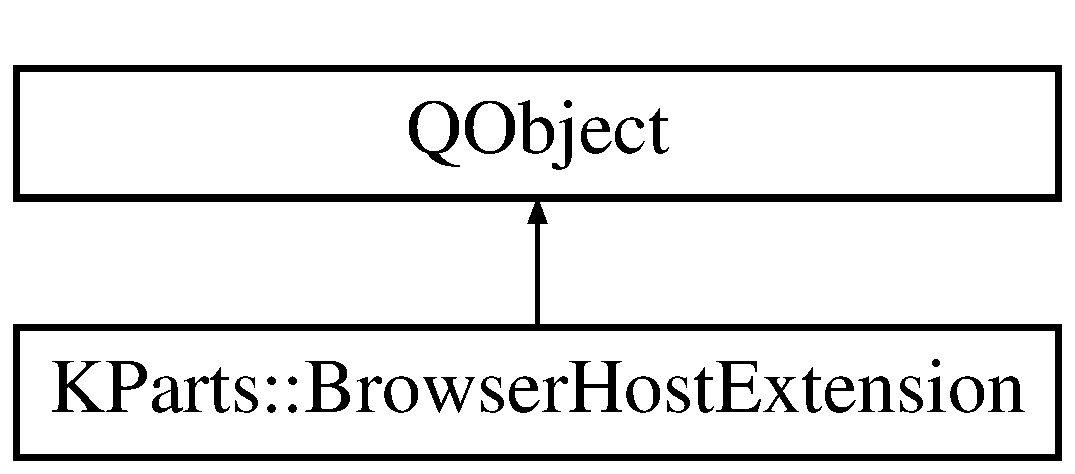
\includegraphics[height=2.000000cm]{classKParts_1_1BrowserHostExtension}
\end{center}
\end{figure}
\subsection*{Public Member Functions}
\begin{DoxyCompactItemize}
\item 
\hyperlink{classKParts_1_1BrowserHostExtension_af1c75309d63462007edd8536c0e57274}{Browser\+Host\+Extension} (\hyperlink{classKParts_1_1ReadOnlyPart}{K\+Parts\+::\+Read\+Only\+Part} $\ast$parent)
\item 
virtual \hyperlink{classKParts_1_1BrowserHostExtension_aa7202fb68e55dcf3556e0611c6b78263}{$\sim$\+Browser\+Host\+Extension} ()
\item 
virtual Q\+String\+List \hyperlink{classKParts_1_1BrowserHostExtension_a25ae4238d3c4f556ee9c7287c16c0f09}{frame\+Names} () const 
\item 
virtual const \hyperlink{classQList}{Q\+List}\\*
$<$ \hyperlink{classKParts_1_1ReadOnlyPart}{K\+Parts\+::\+Read\+Only\+Part} $\ast$ $>$ \hyperlink{classKParts_1_1BrowserHostExtension_a65a6429a794aa78ff5de27f973a43e86}{frames} () const 
\item 
virtual \hyperlink{classKParts_1_1BrowserHostExtension}{Browser\+Host\+Extension} $\ast$ \hyperlink{classKParts_1_1BrowserHostExtension_aa7d6192b9f6a399135f34d530d74a3e7}{find\+Frame\+Parent} (\hyperlink{classKParts_1_1ReadOnlyPart}{K\+Parts\+::\+Read\+Only\+Part} $\ast$calling\+Part, const Q\+String \&frame)
\item 
virtual bool \hyperlink{classKParts_1_1BrowserHostExtension_ae0227348d8b864d3093fb5dc6ca876f0}{open\+Url\+In\+Frame} (const K\+Url \&url, const \hyperlink{classKParts_1_1OpenUrlArguments}{K\+Parts\+::\+Open\+Url\+Arguments} \&arguments, const \hyperlink{structKParts_1_1BrowserArguments}{K\+Parts\+::\+Browser\+Arguments} \&browser\+Arguments)
\end{DoxyCompactItemize}
\subsection*{Static Public Member Functions}
\begin{DoxyCompactItemize}
\item 
static \hyperlink{classKParts_1_1BrowserHostExtension}{Browser\+Host\+Extension} $\ast$ \hyperlink{classKParts_1_1BrowserHostExtension_aa0a695c166742e7f49f65d8a2f3d5216}{child\+Object} (Q\+Object $\ast$obj)
\end{DoxyCompactItemize}


\subsection{Detailed Description}
An extension class for container parts, i.\+e. parts that contain other parts. For instance a K\+H\+T\+M\+L\+Part hosts one part per frame. 

Definition at line 712 of file browserextension.\+h.



\subsection{Constructor \& Destructor Documentation}
\hypertarget{classKParts_1_1BrowserHostExtension_af1c75309d63462007edd8536c0e57274}{\index{K\+Parts\+::\+Browser\+Host\+Extension@{K\+Parts\+::\+Browser\+Host\+Extension}!Browser\+Host\+Extension@{Browser\+Host\+Extension}}
\index{Browser\+Host\+Extension@{Browser\+Host\+Extension}!K\+Parts\+::\+Browser\+Host\+Extension@{K\+Parts\+::\+Browser\+Host\+Extension}}
\subsubsection[{Browser\+Host\+Extension}]{\setlength{\rightskip}{0pt plus 5cm}K\+Parts\+::\+Browser\+Host\+Extension\+::\+Browser\+Host\+Extension (
\begin{DoxyParamCaption}
\item[{{\bf K\+Parts\+::\+Read\+Only\+Part} $\ast$}]{parent}
\end{DoxyParamCaption}
)}}\label{classKParts_1_1BrowserHostExtension_af1c75309d63462007edd8536c0e57274}
\hypertarget{classKParts_1_1BrowserHostExtension_aa7202fb68e55dcf3556e0611c6b78263}{\index{K\+Parts\+::\+Browser\+Host\+Extension@{K\+Parts\+::\+Browser\+Host\+Extension}!````~Browser\+Host\+Extension@{$\sim$\+Browser\+Host\+Extension}}
\index{````~Browser\+Host\+Extension@{$\sim$\+Browser\+Host\+Extension}!K\+Parts\+::\+Browser\+Host\+Extension@{K\+Parts\+::\+Browser\+Host\+Extension}}
\subsubsection[{$\sim$\+Browser\+Host\+Extension}]{\setlength{\rightskip}{0pt plus 5cm}virtual K\+Parts\+::\+Browser\+Host\+Extension\+::$\sim$\+Browser\+Host\+Extension (
\begin{DoxyParamCaption}
{}
\end{DoxyParamCaption}
)\hspace{0.3cm}{\ttfamily [virtual]}}}\label{classKParts_1_1BrowserHostExtension_aa7202fb68e55dcf3556e0611c6b78263}


\subsection{Member Function Documentation}
\hypertarget{classKParts_1_1BrowserHostExtension_aa0a695c166742e7f49f65d8a2f3d5216}{\index{K\+Parts\+::\+Browser\+Host\+Extension@{K\+Parts\+::\+Browser\+Host\+Extension}!child\+Object@{child\+Object}}
\index{child\+Object@{child\+Object}!K\+Parts\+::\+Browser\+Host\+Extension@{K\+Parts\+::\+Browser\+Host\+Extension}}
\subsubsection[{child\+Object}]{\setlength{\rightskip}{0pt plus 5cm}static {\bf Browser\+Host\+Extension}$\ast$ K\+Parts\+::\+Browser\+Host\+Extension\+::child\+Object (
\begin{DoxyParamCaption}
\item[{Q\+Object $\ast$}]{obj}
\end{DoxyParamCaption}
)\hspace{0.3cm}{\ttfamily [static]}}}\label{classKParts_1_1BrowserHostExtension_aa0a695c166742e7f49f65d8a2f3d5216}
Queries {\ttfamily obj} for a child object which inherits from this \hyperlink{classKParts_1_1BrowserHostExtension}{Browser\+Host\+Extension} class. Convenience method. \hypertarget{classKParts_1_1BrowserHostExtension_aa7d6192b9f6a399135f34d530d74a3e7}{\index{K\+Parts\+::\+Browser\+Host\+Extension@{K\+Parts\+::\+Browser\+Host\+Extension}!find\+Frame\+Parent@{find\+Frame\+Parent}}
\index{find\+Frame\+Parent@{find\+Frame\+Parent}!K\+Parts\+::\+Browser\+Host\+Extension@{K\+Parts\+::\+Browser\+Host\+Extension}}
\subsubsection[{find\+Frame\+Parent}]{\setlength{\rightskip}{0pt plus 5cm}virtual {\bf Browser\+Host\+Extension}$\ast$ K\+Parts\+::\+Browser\+Host\+Extension\+::find\+Frame\+Parent (
\begin{DoxyParamCaption}
\item[{{\bf K\+Parts\+::\+Read\+Only\+Part} $\ast$}]{calling\+Part, }
\item[{const Q\+String \&}]{frame}
\end{DoxyParamCaption}
)\hspace{0.3cm}{\ttfamily [virtual]}}}\label{classKParts_1_1BrowserHostExtension_aa7d6192b9f6a399135f34d530d74a3e7}
Returns the part that contains {\ttfamily frame} and that may be accessed by {\ttfamily calling\+Part} \hypertarget{classKParts_1_1BrowserHostExtension_a25ae4238d3c4f556ee9c7287c16c0f09}{\index{K\+Parts\+::\+Browser\+Host\+Extension@{K\+Parts\+::\+Browser\+Host\+Extension}!frame\+Names@{frame\+Names}}
\index{frame\+Names@{frame\+Names}!K\+Parts\+::\+Browser\+Host\+Extension@{K\+Parts\+::\+Browser\+Host\+Extension}}
\subsubsection[{frame\+Names}]{\setlength{\rightskip}{0pt plus 5cm}virtual Q\+String\+List K\+Parts\+::\+Browser\+Host\+Extension\+::frame\+Names (
\begin{DoxyParamCaption}
{}
\end{DoxyParamCaption}
) const\hspace{0.3cm}{\ttfamily [virtual]}}}\label{classKParts_1_1BrowserHostExtension_a25ae4238d3c4f556ee9c7287c16c0f09}
Returns a list of the names of all hosted child objects.

Note that this method does not query the child objects recursively. \hypertarget{classKParts_1_1BrowserHostExtension_a65a6429a794aa78ff5de27f973a43e86}{\index{K\+Parts\+::\+Browser\+Host\+Extension@{K\+Parts\+::\+Browser\+Host\+Extension}!frames@{frames}}
\index{frames@{frames}!K\+Parts\+::\+Browser\+Host\+Extension@{K\+Parts\+::\+Browser\+Host\+Extension}}
\subsubsection[{frames}]{\setlength{\rightskip}{0pt plus 5cm}virtual const {\bf Q\+List}$<${\bf K\+Parts\+::\+Read\+Only\+Part}$\ast$$>$ K\+Parts\+::\+Browser\+Host\+Extension\+::frames (
\begin{DoxyParamCaption}
{}
\end{DoxyParamCaption}
) const\hspace{0.3cm}{\ttfamily [virtual]}}}\label{classKParts_1_1BrowserHostExtension_a65a6429a794aa78ff5de27f973a43e86}
Returns a list of pointers to all hosted child objects.

Note that this method does not query the child objects recursively. \hypertarget{classKParts_1_1BrowserHostExtension_ae0227348d8b864d3093fb5dc6ca876f0}{\index{K\+Parts\+::\+Browser\+Host\+Extension@{K\+Parts\+::\+Browser\+Host\+Extension}!open\+Url\+In\+Frame@{open\+Url\+In\+Frame}}
\index{open\+Url\+In\+Frame@{open\+Url\+In\+Frame}!K\+Parts\+::\+Browser\+Host\+Extension@{K\+Parts\+::\+Browser\+Host\+Extension}}
\subsubsection[{open\+Url\+In\+Frame}]{\setlength{\rightskip}{0pt plus 5cm}virtual bool K\+Parts\+::\+Browser\+Host\+Extension\+::open\+Url\+In\+Frame (
\begin{DoxyParamCaption}
\item[{const K\+Url \&}]{url, }
\item[{const {\bf K\+Parts\+::\+Open\+Url\+Arguments} \&}]{arguments, }
\item[{const {\bf K\+Parts\+::\+Browser\+Arguments} \&}]{browser\+Arguments}
\end{DoxyParamCaption}
)\hspace{0.3cm}{\ttfamily [virtual]}}}\label{classKParts_1_1BrowserHostExtension_ae0227348d8b864d3093fb5dc6ca876f0}
Opens the given url in a hosted child frame. The frame name is specified in the frame\+Name variable in the {\ttfamily browser\+Arguments} parameter (see \hyperlink{structKParts_1_1BrowserArguments}{K\+Parts\+::\+Browser\+Arguments} ) . 

The documentation for this class was generated from the following file\+:\begin{DoxyCompactItemize}
\item 
/usr/include/kparts/\hyperlink{browserextension_8h}{browserextension.\+h}\end{DoxyCompactItemize}

\hypertarget{classKParts_1_1BrowserInterface}{\section{\-K\-Parts\-:\-:\-Browser\-Interface \-Class \-Reference}
\label{classKParts_1_1BrowserInterface}\index{\-K\-Parts\-::\-Browser\-Interface@{\-K\-Parts\-::\-Browser\-Interface}}
}


{\ttfamily \#include $<$browserinterface.\-h$>$}

\subsection*{\-Public \-Member \-Functions}
\begin{DoxyCompactItemize}
\item 
\hyperlink{classKParts_1_1BrowserInterface_a7e7c8ab24a9b90800846028e66eabaed}{\-Browser\-Interface} (\-Q\-Object $\ast$parent)
\item 
virtual \hyperlink{classKParts_1_1BrowserInterface_af6f3ca797d626ffd8676a5babb09ad22}{$\sim$\-Browser\-Interface} ()
\item 
void \hyperlink{classKParts_1_1BrowserInterface_a3b2d9e1791a4a6195b53b48180ec761c}{call\-Method} (const char $\ast$name, const \-Q\-Variant \&argument)
\end{DoxyCompactItemize}


\subsection{\-Detailed \-Description}
\-The purpose of this interface is to allow a direct communication between a \-K\-Part and the hosting browser shell (for example \-Konqueror) . \-A shell implementing this interface can propagate it to embedded kpart components by using the set\-Browser\-Interface call of the part's \hyperlink{classKParts_1_1BrowserExtension}{\-K\-Parts\-::\-Browser\-Extension} object.

\-This interface looks not very rich, but the main functionality is implemented using the call\-Method method for part-\/$>$shell communication and using \-Qt properties for allowing a part to to explicitly query information from the shell.

\-Konqueror in particular, as 'reference' implementation, provides the following functionality through this interface\-:

\-Qt properties\-: \-Q\-\_\-\-P\-R\-O\-P\-E\-R\-T\-Y( uint history\-Length R\-E\-A\-D history\-Length );

\-Callable methods\-: void go\-History( int ); 

\-Definition at line 53 of file browserinterface.\-h.



\subsection{\-Constructor \& \-Destructor \-Documentation}
\hypertarget{classKParts_1_1BrowserInterface_a7e7c8ab24a9b90800846028e66eabaed}{\index{\-K\-Parts\-::\-Browser\-Interface@{\-K\-Parts\-::\-Browser\-Interface}!\-Browser\-Interface@{\-Browser\-Interface}}
\index{\-Browser\-Interface@{\-Browser\-Interface}!KParts::BrowserInterface@{\-K\-Parts\-::\-Browser\-Interface}}
\subsubsection[{\-Browser\-Interface}]{\setlength{\rightskip}{0pt plus 5cm}{\bf \-K\-Parts\-::\-Browser\-Interface\-::\-Browser\-Interface} (
\begin{DoxyParamCaption}
\item[{\-Q\-Object $\ast$}]{parent}
\end{DoxyParamCaption}
)\hspace{0.3cm}{\ttfamily  \mbox{[}explicit\mbox{]}}}}\label{classKParts_1_1BrowserInterface_a7e7c8ab24a9b90800846028e66eabaed}
\hypertarget{classKParts_1_1BrowserInterface_af6f3ca797d626ffd8676a5babb09ad22}{\index{\-K\-Parts\-::\-Browser\-Interface@{\-K\-Parts\-::\-Browser\-Interface}!$\sim$\-Browser\-Interface@{$\sim$\-Browser\-Interface}}
\index{$\sim$\-Browser\-Interface@{$\sim$\-Browser\-Interface}!KParts::BrowserInterface@{\-K\-Parts\-::\-Browser\-Interface}}
\subsubsection[{$\sim$\-Browser\-Interface}]{\setlength{\rightskip}{0pt plus 5cm}virtual {\bf \-K\-Parts\-::\-Browser\-Interface\-::$\sim$\-Browser\-Interface} (
\begin{DoxyParamCaption}
{}
\end{DoxyParamCaption}
)\hspace{0.3cm}{\ttfamily  \mbox{[}virtual\mbox{]}}}}\label{classKParts_1_1BrowserInterface_af6f3ca797d626ffd8676a5babb09ad22}


\subsection{\-Member \-Function \-Documentation}
\hypertarget{classKParts_1_1BrowserInterface_a3b2d9e1791a4a6195b53b48180ec761c}{\index{\-K\-Parts\-::\-Browser\-Interface@{\-K\-Parts\-::\-Browser\-Interface}!call\-Method@{call\-Method}}
\index{call\-Method@{call\-Method}!KParts::BrowserInterface@{\-K\-Parts\-::\-Browser\-Interface}}
\subsubsection[{call\-Method}]{\setlength{\rightskip}{0pt plus 5cm}void {\bf \-K\-Parts\-::\-Browser\-Interface\-::call\-Method} (
\begin{DoxyParamCaption}
\item[{const char $\ast$}]{name, }
\item[{const \-Q\-Variant \&}]{argument}
\end{DoxyParamCaption}
)}}\label{classKParts_1_1BrowserInterface_a3b2d9e1791a4a6195b53b48180ec761c}
\-Perform a dynamic invocation of a method in the \hyperlink{classKParts_1_1BrowserInterface}{\-Browser\-Interface} implementation. \-Methods are to be implemented as simple \-Qt slots. \-You should only include the method name, and not the signature, in the name argument. 

\-The documentation for this class was generated from the following file\-:\begin{DoxyCompactItemize}
\item 
/usr/include/kparts/\hyperlink{browserinterface_8h}{browserinterface.\-h}\end{DoxyCompactItemize}

\hypertarget{classKParts_1_1BrowserOpenOrSaveQuestion}{\section{\-K\-Parts\-:\-:\-Browser\-Open\-Or\-Save\-Question \-Class \-Reference}
\label{classKParts_1_1BrowserOpenOrSaveQuestion}\index{\-K\-Parts\-::\-Browser\-Open\-Or\-Save\-Question@{\-K\-Parts\-::\-Browser\-Open\-Or\-Save\-Question}}
}


{\ttfamily \#include $<$browseropenorsavequestion.\-h$>$}

\subsection*{\-Public \-Types}
\begin{DoxyCompactItemize}
\item 
enum \hyperlink{classKParts_1_1BrowserOpenOrSaveQuestion_a9dfe6a7919cfadff826a357e94ac3a9a}{\-Feature} \{ \hyperlink{classKParts_1_1BrowserOpenOrSaveQuestion_a9dfe6a7919cfadff826a357e94ac3a9aa1cfa50dab189d46bdc4a66c5a1763168}{\-Basic\-Features} =  0, 
\hyperlink{classKParts_1_1BrowserOpenOrSaveQuestion_a9dfe6a7919cfadff826a357e94ac3a9aa3bc1c3177b1a3c8f4cd297ae558c155e}{\-Service\-Selection} =  1
 \}
\item 
enum \hyperlink{classKParts_1_1BrowserOpenOrSaveQuestion_a12842198b7684e9e246e9a207eabc93f}{\-Result} \{ \hyperlink{classKParts_1_1BrowserOpenOrSaveQuestion_a12842198b7684e9e246e9a207eabc93fad5f24b54978bf4ec2a36720d33ad7609}{\-Save}, 
\hyperlink{classKParts_1_1BrowserOpenOrSaveQuestion_a12842198b7684e9e246e9a207eabc93fa1135dc1f27b120bdd6dc83dd7254b60b}{\-Open}, 
\hyperlink{classKParts_1_1BrowserOpenOrSaveQuestion_a12842198b7684e9e246e9a207eabc93fa9038d40b03609466a8433c35b428bf5a}{\-Embed}, 
\hyperlink{classKParts_1_1BrowserOpenOrSaveQuestion_a12842198b7684e9e246e9a207eabc93fac5e1d49f3047805e8f216f11cbe903ab}{\-Cancel}
 \}
\end{DoxyCompactItemize}
\subsection*{\-Public \-Member \-Functions}
\begin{DoxyCompactItemize}
\item 
\hyperlink{classKParts_1_1BrowserOpenOrSaveQuestion_a93097e04518164345d399f7c376b993e}{\-Browser\-Open\-Or\-Save\-Question} (\-Q\-Widget $\ast$parent, const \-K\-Url \&url, const \-Q\-String \&mime\-Type)
\item 
\hyperlink{classKParts_1_1BrowserOpenOrSaveQuestion_a6af2b8e427bf2bb922bb9fcc09df6a65}{$\sim$\-Browser\-Open\-Or\-Save\-Question} ()
\item 
void \hyperlink{classKParts_1_1BrowserOpenOrSaveQuestion_a82733c7818b3c6ee5987ee8c7450c29f}{set\-Suggested\-File\-Name} (const \-Q\-String \&suggested\-File\-Name)
\item 
void \hyperlink{classKParts_1_1BrowserOpenOrSaveQuestion_a998acfa7caa8a47794cc0eb2682a503d}{set\-Features} (\-Features features)
\item 
\hyperlink{classKParts_1_1BrowserOpenOrSaveQuestion_a12842198b7684e9e246e9a207eabc93f}{\-Result} \hyperlink{classKParts_1_1BrowserOpenOrSaveQuestion_a5d9df0d831477073f43071dfe580456d}{ask\-Open\-Or\-Save} ()
\item 
\hyperlink{classKParts_1_1BrowserOpenOrSaveQuestion_a12842198b7684e9e246e9a207eabc93f}{\-Result} \hyperlink{classKParts_1_1BrowserOpenOrSaveQuestion_ad261c14f0e8e32b99b61029fdd5f2fad}{ask\-Embed\-Or\-Save} (int flags=0)
\item 
\-K\-Service\-::\-Ptr \hyperlink{classKParts_1_1BrowserOpenOrSaveQuestion_aaaa2f3a0f18e7acc82152bf296c227da}{selected\-Service} () const 
\end{DoxyCompactItemize}


\subsection{\-Detailed \-Description}
\-This class shows the dialog that asks the user whether to save a url or open a url in another application.

\-It also has the variant which asks \char`\"{}save or embed\char`\"{} (e.\-g. into konqueror).

\begin{DoxySince}{\-Since}
4.\-4 
\end{DoxySince}


\-Definition at line 41 of file browseropenorsavequestion.\-h.



\subsection{\-Member \-Enumeration \-Documentation}
\hypertarget{classKParts_1_1BrowserOpenOrSaveQuestion_a9dfe6a7919cfadff826a357e94ac3a9a}{\index{\-K\-Parts\-::\-Browser\-Open\-Or\-Save\-Question@{\-K\-Parts\-::\-Browser\-Open\-Or\-Save\-Question}!\-Feature@{\-Feature}}
\index{\-Feature@{\-Feature}!KParts::BrowserOpenOrSaveQuestion@{\-K\-Parts\-::\-Browser\-Open\-Or\-Save\-Question}}
\subsubsection[{\-Feature}]{\setlength{\rightskip}{0pt plus 5cm}enum {\bf \-K\-Parts\-::\-Browser\-Open\-Or\-Save\-Question\-::\-Feature}}}\label{classKParts_1_1BrowserOpenOrSaveQuestion_a9dfe6a7919cfadff826a357e94ac3a9a}
\-Set of features that should be enabled in this dialog. \-This allows to add features before making all applications ready for those features (e.\-g. applications need to read \hyperlink{classKParts_1_1BrowserOpenOrSaveQuestion_aaaa2f3a0f18e7acc82152bf296c227da}{selected\-Service()} otherwise the dialog should not show the service selection button) \begin{Desc}
\item[\-Enumerator\-: ]\par
\begin{description}
\index{\-Basic\-Features@{\-Basic\-Features}!\-K\-Parts\-::\-Browser\-Open\-Or\-Save\-Question@{\-K\-Parts\-::\-Browser\-Open\-Or\-Save\-Question}}\index{\-K\-Parts\-::\-Browser\-Open\-Or\-Save\-Question@{\-K\-Parts\-::\-Browser\-Open\-Or\-Save\-Question}!\-Basic\-Features@{\-Basic\-Features}}\item[{\em 
\hypertarget{classKParts_1_1BrowserOpenOrSaveQuestion_a9dfe6a7919cfadff826a357e94ac3a9aa1cfa50dab189d46bdc4a66c5a1763168}{\-Basic\-Features}\label{classKParts_1_1BrowserOpenOrSaveQuestion_a9dfe6a7919cfadff826a357e94ac3a9aa1cfa50dab189d46bdc4a66c5a1763168}
}]\-Only the basic save, open, embed, cancel button \index{\-Service\-Selection@{\-Service\-Selection}!\-K\-Parts\-::\-Browser\-Open\-Or\-Save\-Question@{\-K\-Parts\-::\-Browser\-Open\-Or\-Save\-Question}}\index{\-K\-Parts\-::\-Browser\-Open\-Or\-Save\-Question@{\-K\-Parts\-::\-Browser\-Open\-Or\-Save\-Question}!\-Service\-Selection@{\-Service\-Selection}}\item[{\em 
\hypertarget{classKParts_1_1BrowserOpenOrSaveQuestion_a9dfe6a7919cfadff826a357e94ac3a9aa3bc1c3177b1a3c8f4cd297ae558c155e}{\-Service\-Selection}\label{classKParts_1_1BrowserOpenOrSaveQuestion_a9dfe6a7919cfadff826a357e94ac3a9aa3bc1c3177b1a3c8f4cd297ae558c155e}
}]\-Shows \char`\"{}\-Open With...\char`\"{} with the associated applications for the mimetype \end{description}
\end{Desc}



\-Definition at line 64 of file browseropenorsavequestion.\-h.


\begin{DoxyCode}
                 { BasicFeatures = 0, 
                   ServiceSelection = 1 
    };
\end{DoxyCode}
\hypertarget{classKParts_1_1BrowserOpenOrSaveQuestion_a12842198b7684e9e246e9a207eabc93f}{\index{\-K\-Parts\-::\-Browser\-Open\-Or\-Save\-Question@{\-K\-Parts\-::\-Browser\-Open\-Or\-Save\-Question}!\-Result@{\-Result}}
\index{\-Result@{\-Result}!KParts::BrowserOpenOrSaveQuestion@{\-K\-Parts\-::\-Browser\-Open\-Or\-Save\-Question}}
\subsubsection[{\-Result}]{\setlength{\rightskip}{0pt plus 5cm}enum {\bf \-K\-Parts\-::\-Browser\-Open\-Or\-Save\-Question\-::\-Result}}}\label{classKParts_1_1BrowserOpenOrSaveQuestion_a12842198b7684e9e246e9a207eabc93f}
\begin{Desc}
\item[\-Enumerator\-: ]\par
\begin{description}
\index{\-Save@{\-Save}!\-K\-Parts\-::\-Browser\-Open\-Or\-Save\-Question@{\-K\-Parts\-::\-Browser\-Open\-Or\-Save\-Question}}\index{\-K\-Parts\-::\-Browser\-Open\-Or\-Save\-Question@{\-K\-Parts\-::\-Browser\-Open\-Or\-Save\-Question}!\-Save@{\-Save}}\item[{\em 
\hypertarget{classKParts_1_1BrowserOpenOrSaveQuestion_a12842198b7684e9e246e9a207eabc93fad5f24b54978bf4ec2a36720d33ad7609}{\-Save}\label{classKParts_1_1BrowserOpenOrSaveQuestion_a12842198b7684e9e246e9a207eabc93fad5f24b54978bf4ec2a36720d33ad7609}
}]\index{\-Open@{\-Open}!\-K\-Parts\-::\-Browser\-Open\-Or\-Save\-Question@{\-K\-Parts\-::\-Browser\-Open\-Or\-Save\-Question}}\index{\-K\-Parts\-::\-Browser\-Open\-Or\-Save\-Question@{\-K\-Parts\-::\-Browser\-Open\-Or\-Save\-Question}!\-Open@{\-Open}}\item[{\em 
\hypertarget{classKParts_1_1BrowserOpenOrSaveQuestion_a12842198b7684e9e246e9a207eabc93fa1135dc1f27b120bdd6dc83dd7254b60b}{\-Open}\label{classKParts_1_1BrowserOpenOrSaveQuestion_a12842198b7684e9e246e9a207eabc93fa1135dc1f27b120bdd6dc83dd7254b60b}
}]\index{\-Embed@{\-Embed}!\-K\-Parts\-::\-Browser\-Open\-Or\-Save\-Question@{\-K\-Parts\-::\-Browser\-Open\-Or\-Save\-Question}}\index{\-K\-Parts\-::\-Browser\-Open\-Or\-Save\-Question@{\-K\-Parts\-::\-Browser\-Open\-Or\-Save\-Question}!\-Embed@{\-Embed}}\item[{\em 
\hypertarget{classKParts_1_1BrowserOpenOrSaveQuestion_a12842198b7684e9e246e9a207eabc93fa9038d40b03609466a8433c35b428bf5a}{\-Embed}\label{classKParts_1_1BrowserOpenOrSaveQuestion_a12842198b7684e9e246e9a207eabc93fa9038d40b03609466a8433c35b428bf5a}
}]\index{\-Cancel@{\-Cancel}!\-K\-Parts\-::\-Browser\-Open\-Or\-Save\-Question@{\-K\-Parts\-::\-Browser\-Open\-Or\-Save\-Question}}\index{\-K\-Parts\-::\-Browser\-Open\-Or\-Save\-Question@{\-K\-Parts\-::\-Browser\-Open\-Or\-Save\-Question}!\-Cancel@{\-Cancel}}\item[{\em 
\hypertarget{classKParts_1_1BrowserOpenOrSaveQuestion_a12842198b7684e9e246e9a207eabc93fac5e1d49f3047805e8f216f11cbe903ab}{\-Cancel}\label{classKParts_1_1BrowserOpenOrSaveQuestion_a12842198b7684e9e246e9a207eabc93fac5e1d49f3047805e8f216f11cbe903ab}
}]\end{description}
\end{Desc}



\-Definition at line 74 of file browseropenorsavequestion.\-h.


\begin{DoxyCode}
{ Save, Open, Embed, Cancel };
\end{DoxyCode}


\subsection{\-Constructor \& \-Destructor \-Documentation}
\hypertarget{classKParts_1_1BrowserOpenOrSaveQuestion_a93097e04518164345d399f7c376b993e}{\index{\-K\-Parts\-::\-Browser\-Open\-Or\-Save\-Question@{\-K\-Parts\-::\-Browser\-Open\-Or\-Save\-Question}!\-Browser\-Open\-Or\-Save\-Question@{\-Browser\-Open\-Or\-Save\-Question}}
\index{\-Browser\-Open\-Or\-Save\-Question@{\-Browser\-Open\-Or\-Save\-Question}!KParts::BrowserOpenOrSaveQuestion@{\-K\-Parts\-::\-Browser\-Open\-Or\-Save\-Question}}
\subsubsection[{\-Browser\-Open\-Or\-Save\-Question}]{\setlength{\rightskip}{0pt plus 5cm}{\bf \-K\-Parts\-::\-Browser\-Open\-Or\-Save\-Question\-::\-Browser\-Open\-Or\-Save\-Question} (
\begin{DoxyParamCaption}
\item[{\-Q\-Widget $\ast$}]{parent, }
\item[{const \-K\-Url \&}]{url, }
\item[{const \-Q\-String \&}]{mime\-Type}
\end{DoxyParamCaption}
)}}\label{classKParts_1_1BrowserOpenOrSaveQuestion_a93097e04518164345d399f7c376b993e}
\-Constructor, for all kinds of dialogs shown in this class. 
\begin{DoxyParams}{\-Parameters}
{\em url} & the \-U\-R\-L in question \\
\hline
{\em mime\-Type} & the mimetype of the \-U\-R\-L \\
\hline
\end{DoxyParams}
\hypertarget{classKParts_1_1BrowserOpenOrSaveQuestion_a6af2b8e427bf2bb922bb9fcc09df6a65}{\index{\-K\-Parts\-::\-Browser\-Open\-Or\-Save\-Question@{\-K\-Parts\-::\-Browser\-Open\-Or\-Save\-Question}!$\sim$\-Browser\-Open\-Or\-Save\-Question@{$\sim$\-Browser\-Open\-Or\-Save\-Question}}
\index{$\sim$\-Browser\-Open\-Or\-Save\-Question@{$\sim$\-Browser\-Open\-Or\-Save\-Question}!KParts::BrowserOpenOrSaveQuestion@{\-K\-Parts\-::\-Browser\-Open\-Or\-Save\-Question}}
\subsubsection[{$\sim$\-Browser\-Open\-Or\-Save\-Question}]{\setlength{\rightskip}{0pt plus 5cm}{\bf \-K\-Parts\-::\-Browser\-Open\-Or\-Save\-Question\-::$\sim$\-Browser\-Open\-Or\-Save\-Question} (
\begin{DoxyParamCaption}
{}
\end{DoxyParamCaption}
)}}\label{classKParts_1_1BrowserOpenOrSaveQuestion_a6af2b8e427bf2bb922bb9fcc09df6a65}


\subsection{\-Member \-Function \-Documentation}
\hypertarget{classKParts_1_1BrowserOpenOrSaveQuestion_ad261c14f0e8e32b99b61029fdd5f2fad}{\index{\-K\-Parts\-::\-Browser\-Open\-Or\-Save\-Question@{\-K\-Parts\-::\-Browser\-Open\-Or\-Save\-Question}!ask\-Embed\-Or\-Save@{ask\-Embed\-Or\-Save}}
\index{ask\-Embed\-Or\-Save@{ask\-Embed\-Or\-Save}!KParts::BrowserOpenOrSaveQuestion@{\-K\-Parts\-::\-Browser\-Open\-Or\-Save\-Question}}
\subsubsection[{ask\-Embed\-Or\-Save}]{\setlength{\rightskip}{0pt plus 5cm}{\bf \-Result} {\bf \-K\-Parts\-::\-Browser\-Open\-Or\-Save\-Question\-::ask\-Embed\-Or\-Save} (
\begin{DoxyParamCaption}
\item[{int}]{flags = {\ttfamily 0}}
\end{DoxyParamCaption}
)}}\label{classKParts_1_1BrowserOpenOrSaveQuestion_ad261c14f0e8e32b99b61029fdd5f2fad}
\-Ask the user whether to save or open a url in another application. 
\begin{DoxyParams}{\-Parameters}
{\em parent} & parent widget for the dialog \\
\hline
{\em flags} & set to \hyperlink{classKParts_1_1BrowserRun_ae78b4e6186491175ccdb4b0f2693c08daa236cc4b09fc3ca6f88d9a37b32ea8af}{\-Browser\-Run\-::\-Attachment\-Disposition} if suggested by the server \-This is used because by default text/html files are opened embedded in browsers, not saved. \-But if the server said \char`\"{}attachment\char`\"{}, it means the user is download a file for saving it. \\
\hline
\end{DoxyParams}
\begin{DoxyReturn}{\-Returns}
\-Save, \-Embed or \-Cancel. 
\end{DoxyReturn}
\hypertarget{classKParts_1_1BrowserOpenOrSaveQuestion_a5d9df0d831477073f43071dfe580456d}{\index{\-K\-Parts\-::\-Browser\-Open\-Or\-Save\-Question@{\-K\-Parts\-::\-Browser\-Open\-Or\-Save\-Question}!ask\-Open\-Or\-Save@{ask\-Open\-Or\-Save}}
\index{ask\-Open\-Or\-Save@{ask\-Open\-Or\-Save}!KParts::BrowserOpenOrSaveQuestion@{\-K\-Parts\-::\-Browser\-Open\-Or\-Save\-Question}}
\subsubsection[{ask\-Open\-Or\-Save}]{\setlength{\rightskip}{0pt plus 5cm}{\bf \-Result} {\bf \-K\-Parts\-::\-Browser\-Open\-Or\-Save\-Question\-::ask\-Open\-Or\-Save} (
\begin{DoxyParamCaption}
{}
\end{DoxyParamCaption}
)}}\label{classKParts_1_1BrowserOpenOrSaveQuestion_a5d9df0d831477073f43071dfe580456d}
\-Ask the user whether to save or open a url in another application. 
\begin{DoxyParams}{\-Parameters}
{\em parent} & parent widget for the dialog \\
\hline
\end{DoxyParams}
\begin{DoxyReturn}{\-Returns}
\-Save, \-Open or \-Cancel. 
\end{DoxyReturn}
\hypertarget{classKParts_1_1BrowserOpenOrSaveQuestion_aaaa2f3a0f18e7acc82152bf296c227da}{\index{\-K\-Parts\-::\-Browser\-Open\-Or\-Save\-Question@{\-K\-Parts\-::\-Browser\-Open\-Or\-Save\-Question}!selected\-Service@{selected\-Service}}
\index{selected\-Service@{selected\-Service}!KParts::BrowserOpenOrSaveQuestion@{\-K\-Parts\-::\-Browser\-Open\-Or\-Save\-Question}}
\subsubsection[{selected\-Service}]{\setlength{\rightskip}{0pt plus 5cm}\-K\-Service\-::\-Ptr {\bf \-K\-Parts\-::\-Browser\-Open\-Or\-Save\-Question\-::selected\-Service} (
\begin{DoxyParamCaption}
{}
\end{DoxyParamCaption}
) const}}\label{classKParts_1_1BrowserOpenOrSaveQuestion_aaaa2f3a0f18e7acc82152bf296c227da}
\begin{DoxyReturn}{\-Returns}
the service that was selected during ask\-Open\-Or\-Save, if it returned \-Open. \-In all other cases (no associated application, \-Save or \-Cancel selected), this returns 0.
\end{DoxyReturn}
\-Requires set\-Features(\-Browser\-Open\-Or\-Save\-Question\-::\-Service\-Selection). \hypertarget{classKParts_1_1BrowserOpenOrSaveQuestion_a998acfa7caa8a47794cc0eb2682a503d}{\index{\-K\-Parts\-::\-Browser\-Open\-Or\-Save\-Question@{\-K\-Parts\-::\-Browser\-Open\-Or\-Save\-Question}!set\-Features@{set\-Features}}
\index{set\-Features@{set\-Features}!KParts::BrowserOpenOrSaveQuestion@{\-K\-Parts\-::\-Browser\-Open\-Or\-Save\-Question}}
\subsubsection[{set\-Features}]{\setlength{\rightskip}{0pt plus 5cm}void {\bf \-K\-Parts\-::\-Browser\-Open\-Or\-Save\-Question\-::set\-Features} (
\begin{DoxyParamCaption}
\item[{\-Features}]{features}
\end{DoxyParamCaption}
)}}\label{classKParts_1_1BrowserOpenOrSaveQuestion_a998acfa7caa8a47794cc0eb2682a503d}
\-Enables the given features in the dialog \hypertarget{classKParts_1_1BrowserOpenOrSaveQuestion_a82733c7818b3c6ee5987ee8c7450c29f}{\index{\-K\-Parts\-::\-Browser\-Open\-Or\-Save\-Question@{\-K\-Parts\-::\-Browser\-Open\-Or\-Save\-Question}!set\-Suggested\-File\-Name@{set\-Suggested\-File\-Name}}
\index{set\-Suggested\-File\-Name@{set\-Suggested\-File\-Name}!KParts::BrowserOpenOrSaveQuestion@{\-K\-Parts\-::\-Browser\-Open\-Or\-Save\-Question}}
\subsubsection[{set\-Suggested\-File\-Name}]{\setlength{\rightskip}{0pt plus 5cm}void {\bf \-K\-Parts\-::\-Browser\-Open\-Or\-Save\-Question\-::set\-Suggested\-File\-Name} (
\begin{DoxyParamCaption}
\item[{const \-Q\-String \&}]{suggested\-File\-Name}
\end{DoxyParamCaption}
)}}\label{classKParts_1_1BrowserOpenOrSaveQuestion_a82733c7818b3c6ee5987ee8c7450c29f}
\-Sets the suggested filename, shown in the dialog. 
\begin{DoxyParams}{\-Parameters}
{\em suggested\-File\-Name} & optional file name suggested by the server (\-H\-T\-T\-P \-Content-\/\-Disposition) \\
\hline
\end{DoxyParams}


\-The documentation for this class was generated from the following file\-:\begin{DoxyCompactItemize}
\item 
/usr/include/kparts/\hyperlink{browseropenorsavequestion_8h}{browseropenorsavequestion.\-h}\end{DoxyCompactItemize}

\hypertarget{classKParts_1_1BrowserRun}{\section{K\+Parts\+:\+:Browser\+Run Class Reference}
\label{classKParts_1_1BrowserRun}\index{K\+Parts\+::\+Browser\+Run@{K\+Parts\+::\+Browser\+Run}}
}


{\ttfamily \#include $<$browserrun.\+h$>$}

Inheritance diagram for K\+Parts\+:\+:Browser\+Run\+:\begin{figure}[H]
\begin{center}
\leavevmode
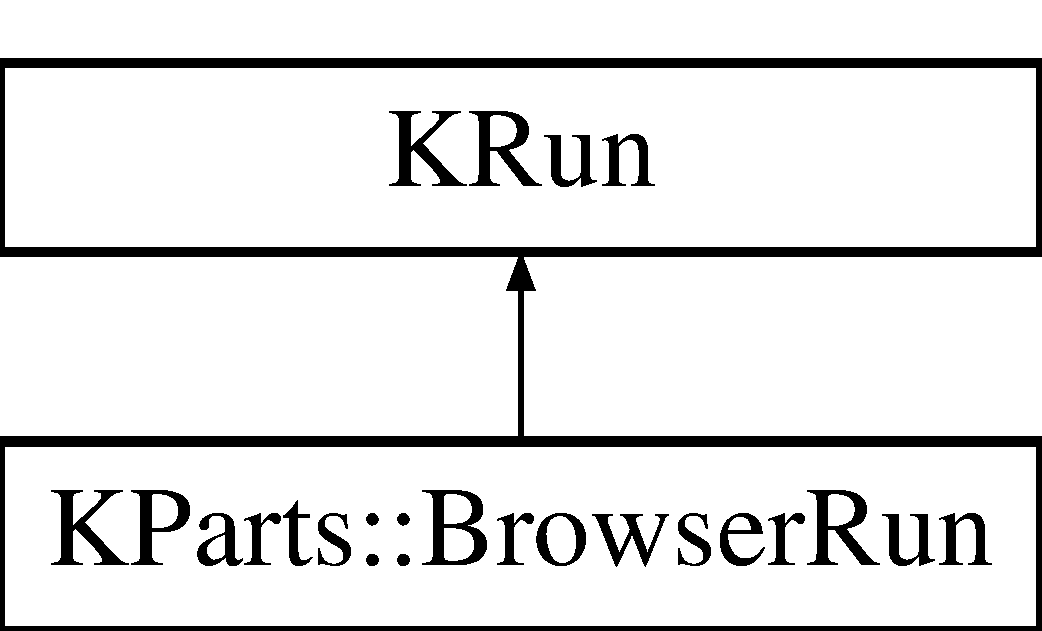
\includegraphics[height=2.000000cm]{classKParts_1_1BrowserRun}
\end{center}
\end{figure}
\subsection*{Public Types}
\begin{DoxyCompactItemize}
\item 
enum \hyperlink{classKParts_1_1BrowserRun_a32ee53f65c723ec01f4c4c28e91db8e6}{Ask\+Save\+Result} \{ \hyperlink{classKParts_1_1BrowserRun_a32ee53f65c723ec01f4c4c28e91db8e6adc6aa058c60662f393aa8168681d8a58}{Save}, 
\hyperlink{classKParts_1_1BrowserRun_a32ee53f65c723ec01f4c4c28e91db8e6ac44e1cbf269e6df9367051c7561de90b}{Open}, 
\hyperlink{classKParts_1_1BrowserRun_a32ee53f65c723ec01f4c4c28e91db8e6aea88673d252dcf7b37559606ce45667f}{Cancel}
 \}
\item 
enum \hyperlink{classKParts_1_1BrowserRun_ae78b4e6186491175ccdb4b0f2693c08d}{Ask\+Embed\+Or\+Save\+Flags} \{ \hyperlink{classKParts_1_1BrowserRun_ae78b4e6186491175ccdb4b0f2693c08dafa80faaf171d25b4a0e095a2c1f51cfe}{Inline\+Disposition} = 0, 
\hyperlink{classKParts_1_1BrowserRun_ae78b4e6186491175ccdb4b0f2693c08daa236cc4b09fc3ca6f88d9a37b32ea8af}{Attachment\+Disposition} = 1
 \}
\end{DoxyCompactItemize}
\subsection*{Public Member Functions}
\begin{DoxyCompactItemize}
\item 
\hyperlink{classKParts_1_1BrowserRun_a48308a3cd53da552fb60a86400d06228}{Browser\+Run} (const K\+Url \&\hyperlink{classKParts_1_1BrowserRun_ad3f7d10647ab8b5a77399f46df92046b}{url}, const \hyperlink{classKParts_1_1OpenUrlArguments}{K\+Parts\+::\+Open\+Url\+Arguments} \&args, const \hyperlink{structKParts_1_1BrowserArguments}{K\+Parts\+::\+Browser\+Arguments} \&browser\+Args, \hyperlink{classKParts_1_1ReadOnlyPart}{K\+Parts\+::\+Read\+Only\+Part} $\ast$\hyperlink{classKParts_1_1BrowserRun_a65886b4004c00ddcc08b976f1042d0dc}{part}, Q\+Widget $\ast$window, bool remove\+Referrer, bool trusted\+Source, bool \hyperlink{classKParts_1_1BrowserRun_a1caa242a8389d61d6758e25a68f9df50}{hide\+Error\+Dialog}=false)
\item 
virtual \hyperlink{classKParts_1_1BrowserRun_aa141423e9096f956970d4fe92e581814}{$\sim$\+Browser\+Run} ()
\item 
\hyperlink{classKParts_1_1OpenUrlArguments}{K\+Parts\+::\+Open\+Url\+Arguments} \& \hyperlink{classKParts_1_1BrowserRun_a5843399feb9cafe9a2f62b258c2f5a31}{arguments} ()
\item 
\hyperlink{structKParts_1_1BrowserArguments}{K\+Parts\+::\+Browser\+Arguments} \& \hyperlink{classKParts_1_1BrowserRun_a7fb44c1871cf67132853d8bb59dfe006}{browser\+Arguments} ()
\item 
\hyperlink{classKParts_1_1ReadOnlyPart}{K\+Parts\+::\+Read\+Only\+Part} $\ast$ \hyperlink{classKParts_1_1BrowserRun_a65886b4004c00ddcc08b976f1042d0dc}{part} () const 
\item 
K\+Url \hyperlink{classKParts_1_1BrowserRun_ad3f7d10647ab8b5a77399f46df92046b}{url} () const 
\item 
bool \hyperlink{classKParts_1_1BrowserRun_a1caa242a8389d61d6758e25a68f9df50}{hide\+Error\+Dialog} () const 
\item 
Q\+String \hyperlink{classKParts_1_1BrowserRun_aa0ffe2da032f4e14eb6c7ba5f0d9996f}{content\+Disposition} () const 
\item 
bool \hyperlink{classKParts_1_1BrowserRun_a7daa3c6e44b8a37aa9c1d010972194dc}{server\+Suggests\+Save} () const 
\item 
virtual void \hyperlink{classKParts_1_1BrowserRun_acff594a6127fe8f5f19364e1da47eccf}{save} (const K\+Url \&\hyperlink{classKParts_1_1BrowserRun_ad3f7d10647ab8b5a77399f46df92046b}{url}, const Q\+String \&suggested\+File\+Name)
\end{DoxyCompactItemize}
\subsection*{Static Public Member Functions}
\begin{DoxyCompactItemize}
\item 
static K\+D\+E\+\_\+\+D\+E\+P\+R\+E\+C\+A\+T\+E\+D \hyperlink{classKParts_1_1BrowserRun_a32ee53f65c723ec01f4c4c28e91db8e6}{Ask\+Save\+Result} \hyperlink{classKParts_1_1BrowserRun_a240c17aac1cd740315731916f0616723}{ask\+Save} (const K\+Url \&\hyperlink{classKParts_1_1BrowserRun_ad3f7d10647ab8b5a77399f46df92046b}{url}, K\+Service\+::\+Ptr offer, const Q\+String \&mime\+Type, const Q\+String \&suggested\+File\+Name=Q\+String())
\item 
static K\+D\+E\+\_\+\+D\+E\+P\+R\+E\+C\+A\+T\+E\+D \hyperlink{classKParts_1_1BrowserRun_a32ee53f65c723ec01f4c4c28e91db8e6}{Ask\+Save\+Result} \hyperlink{classKParts_1_1BrowserRun_a548576ed0ee79c29f1b68d16922ae6bd}{ask\+Embed\+Or\+Save} (const K\+Url \&\hyperlink{classKParts_1_1BrowserRun_ad3f7d10647ab8b5a77399f46df92046b}{url}, const Q\+String \&mime\+Type, const Q\+String \&suggested\+File\+Name=Q\+String(), int flags=0)
\item 
static void \hyperlink{classKParts_1_1BrowserRun_a38a97c58c4a3bb15e3de9e5cdf7fb24a}{simple\+Save} (const K\+Url \&\hyperlink{classKParts_1_1BrowserRun_ad3f7d10647ab8b5a77399f46df92046b}{url}, const Q\+String \&suggested\+File\+Name, Q\+Widget $\ast$window=0)
\item 
static void \hyperlink{classKParts_1_1BrowserRun_a75d80364750fd734cabccaa8a818a48d}{save\+Url} (const K\+Url \&\hyperlink{classKParts_1_1BrowserRun_ad3f7d10647ab8b5a77399f46df92046b}{url}, const Q\+String \&suggested\+File\+Name, Q\+Widget $\ast$window, const \hyperlink{classKParts_1_1OpenUrlArguments}{K\+Parts\+::\+Open\+Url\+Arguments} \&args)
\item 
static void \hyperlink{classKParts_1_1BrowserRun_a76f09a0166b39cf15e02df97765d8d0a}{save\+Url\+Using\+K\+I\+O} (const K\+Url \&src\+Url, const K\+Url \&dest\+Url, Q\+Widget $\ast$window, const \hyperlink{classQMap}{Q\+Map}$<$ Q\+String, Q\+String $>$ \&meta\+Data)
\item 
static bool \hyperlink{classKParts_1_1BrowserRun_adc6f66d941b8361b6808f4d6dcee312b}{allow\+Execution} (const Q\+String \&mime\+Type, const K\+Url \&\hyperlink{classKParts_1_1BrowserRun_ad3f7d10647ab8b5a77399f46df92046b}{url})
\item 
static bool \hyperlink{classKParts_1_1BrowserRun_a5e9221ceeeaddac5b6f0929c9298afa6}{is\+Text\+Executable} (const Q\+String \&mime\+Type)
\item 
static K\+Url \hyperlink{classKParts_1_1BrowserRun_a07ae3b98d8050e48980711788c2b84d8}{make\+Error\+Url} (int error, const Q\+String \&error\+Text, const Q\+String \&initial\+Url)
\end{DoxyCompactItemize}
\subsection*{Protected Types}
\begin{DoxyCompactItemize}
\item 
enum \hyperlink{classKParts_1_1BrowserRun_af7f4f75d5ab28c3183f9f5ee96b8a79f}{Non\+Embeddable\+Result} \{ \hyperlink{classKParts_1_1BrowserRun_af7f4f75d5ab28c3183f9f5ee96b8a79fa1489069cb381b59c2de0d501e347388e}{Handled}, 
\hyperlink{classKParts_1_1BrowserRun_af7f4f75d5ab28c3183f9f5ee96b8a79fae968cb6de73d4c96f7644a55adf610ca}{Not\+Handled}, 
\hyperlink{classKParts_1_1BrowserRun_af7f4f75d5ab28c3183f9f5ee96b8a79fa7a4f366bf6b4319caab0e48610f5e26c}{Delayed}
 \}
\end{DoxyCompactItemize}
\subsection*{Protected Slots}
\begin{DoxyCompactItemize}
\item 
void \hyperlink{classKParts_1_1BrowserRun_abed6cac6df3f2147be76a0524e92ddc1}{slot\+Browser\+Scan\+Finished} (K\+Job $\ast$job)
\item 
void \hyperlink{classKParts_1_1BrowserRun_a549306dfbb92c12c97a1663b82d93a51}{slot\+Browser\+Mimetype} (K\+I\+O\+::\+Job $\ast$job, const Q\+String \&type)
\item 
void \hyperlink{classKParts_1_1BrowserRun_a43d7f0c6a27c25ba93d6085162574d7e}{slot\+Copy\+To\+Temp\+File\+Result} (K\+Job $\ast$job)
\item 
virtual void \hyperlink{classKParts_1_1BrowserRun_a27fc9f400c6eccf2188d5899550af89a}{slot\+Stat\+Result} (K\+Job $\ast$job)
\end{DoxyCompactItemize}
\subsection*{Protected Member Functions}
\begin{DoxyCompactItemize}
\item 
virtual void \hyperlink{classKParts_1_1BrowserRun_a78858ebd1b73ece426abc128edf4e4e5}{scan\+File} ()
\item 
virtual void \hyperlink{classKParts_1_1BrowserRun_a6140fdc2848021232a3c84a5df98b130}{init} ()
\item 
virtual void \hyperlink{classKParts_1_1BrowserRun_a2b961dffc73904a1b7fde816a49bb05f}{handle\+Error} (K\+Job $\ast$job)
\item 
\hyperlink{classKParts_1_1BrowserRun_af7f4f75d5ab28c3183f9f5ee96b8a79f}{Non\+Embeddable\+Result} \hyperlink{classKParts_1_1BrowserRun_ad1b275632b2bc76378879a15ac548706}{handle\+Non\+Embeddable} (const Q\+String \&mime\+Type)
\item 
\hyperlink{classKParts_1_1BrowserRun_af7f4f75d5ab28c3183f9f5ee96b8a79f}{Non\+Embeddable\+Result} \hyperlink{classKParts_1_1BrowserRun_a7fbb390d0f47884e704ebe77f5148808}{handle\+Non\+Embeddable} (const Q\+String \&mime\+Type, K\+Service\+::\+Ptr $\ast$p\+Selected\+Service)
\end{DoxyCompactItemize}


\subsection{Detailed Description}
This class extends K\+Run to provide additional functionality for browsers\+:
\begin{DoxyItemize}
\item \char`\"{}save or open\char`\"{} dialog boxes
\item \char`\"{}save\char`\"{} functionality
\item support for H\+T\+T\+P P\+O\+S\+T (including saving the result to a temp file if opening a separate application)
\item warning before launching executables off the web
\item custom error handling (i.\+e. treating errors as H\+T\+M\+L pages)
\item generation of S\+S\+L metadata depending on the previous U\+R\+L shown by the part \begin{DoxyAuthor}{Author}
David Faure \href{mailto:faure@kde.org}{\tt faure@kde.\+org} 
\end{DoxyAuthor}

\end{DoxyItemize}

Definition at line 39 of file browserrun.\+h.



\subsection{Member Enumeration Documentation}
\hypertarget{classKParts_1_1BrowserRun_ae78b4e6186491175ccdb4b0f2693c08d}{\index{K\+Parts\+::\+Browser\+Run@{K\+Parts\+::\+Browser\+Run}!Ask\+Embed\+Or\+Save\+Flags@{Ask\+Embed\+Or\+Save\+Flags}}
\index{Ask\+Embed\+Or\+Save\+Flags@{Ask\+Embed\+Or\+Save\+Flags}!K\+Parts\+::\+Browser\+Run@{K\+Parts\+::\+Browser\+Run}}
\subsubsection[{Ask\+Embed\+Or\+Save\+Flags}]{\setlength{\rightskip}{0pt plus 5cm}enum {\bf K\+Parts\+::\+Browser\+Run\+::\+Ask\+Embed\+Or\+Save\+Flags}}}\label{classKParts_1_1BrowserRun_ae78b4e6186491175ccdb4b0f2693c08d}
\begin{Desc}
\item[Enumerator]\par
\begin{description}
\index{Inline\+Disposition@{Inline\+Disposition}!K\+Parts\+::\+Browser\+Run@{K\+Parts\+::\+Browser\+Run}}\index{K\+Parts\+::\+Browser\+Run@{K\+Parts\+::\+Browser\+Run}!Inline\+Disposition@{Inline\+Disposition}}\item[{\em 
\hypertarget{classKParts_1_1BrowserRun_ae78b4e6186491175ccdb4b0f2693c08dafa80faaf171d25b4a0e095a2c1f51cfe}{Inline\+Disposition}\label{classKParts_1_1BrowserRun_ae78b4e6186491175ccdb4b0f2693c08dafa80faaf171d25b4a0e095a2c1f51cfe}
}]\index{Attachment\+Disposition@{Attachment\+Disposition}!K\+Parts\+::\+Browser\+Run@{K\+Parts\+::\+Browser\+Run}}\index{K\+Parts\+::\+Browser\+Run@{K\+Parts\+::\+Browser\+Run}!Attachment\+Disposition@{Attachment\+Disposition}}\item[{\em 
\hypertarget{classKParts_1_1BrowserRun_ae78b4e6186491175ccdb4b0f2693c08daa236cc4b09fc3ca6f88d9a37b32ea8af}{Attachment\+Disposition}\label{classKParts_1_1BrowserRun_ae78b4e6186491175ccdb4b0f2693c08daa236cc4b09fc3ca6f88d9a37b32ea8af}
}]\end{description}
\end{Desc}


Definition at line 98 of file browserrun.\+h.


\begin{DoxyCode}
98 \{ \hyperlink{classKParts_1_1BrowserRun_ae78b4e6186491175ccdb4b0f2693c08dafa80faaf171d25b4a0e095a2c1f51cfe}{InlineDisposition} = 0, \hyperlink{classKParts_1_1BrowserRun_ae78b4e6186491175ccdb4b0f2693c08daa236cc4b09fc3ca6f88d9a37b32ea8af}{AttachmentDisposition} = 1 \};
\end{DoxyCode}
\hypertarget{classKParts_1_1BrowserRun_a32ee53f65c723ec01f4c4c28e91db8e6}{\index{K\+Parts\+::\+Browser\+Run@{K\+Parts\+::\+Browser\+Run}!Ask\+Save\+Result@{Ask\+Save\+Result}}
\index{Ask\+Save\+Result@{Ask\+Save\+Result}!K\+Parts\+::\+Browser\+Run@{K\+Parts\+::\+Browser\+Run}}
\subsubsection[{Ask\+Save\+Result}]{\setlength{\rightskip}{0pt plus 5cm}enum {\bf K\+Parts\+::\+Browser\+Run\+::\+Ask\+Save\+Result}}}\label{classKParts_1_1BrowserRun_a32ee53f65c723ec01f4c4c28e91db8e6}
\begin{Desc}
\item[Enumerator]\par
\begin{description}
\index{Save@{Save}!K\+Parts\+::\+Browser\+Run@{K\+Parts\+::\+Browser\+Run}}\index{K\+Parts\+::\+Browser\+Run@{K\+Parts\+::\+Browser\+Run}!Save@{Save}}\item[{\em 
\hypertarget{classKParts_1_1BrowserRun_a32ee53f65c723ec01f4c4c28e91db8e6adc6aa058c60662f393aa8168681d8a58}{Save}\label{classKParts_1_1BrowserRun_a32ee53f65c723ec01f4c4c28e91db8e6adc6aa058c60662f393aa8168681d8a58}
}]\index{Open@{Open}!K\+Parts\+::\+Browser\+Run@{K\+Parts\+::\+Browser\+Run}}\index{K\+Parts\+::\+Browser\+Run@{K\+Parts\+::\+Browser\+Run}!Open@{Open}}\item[{\em 
\hypertarget{classKParts_1_1BrowserRun_a32ee53f65c723ec01f4c4c28e91db8e6ac44e1cbf269e6df9367051c7561de90b}{Open}\label{classKParts_1_1BrowserRun_a32ee53f65c723ec01f4c4c28e91db8e6ac44e1cbf269e6df9367051c7561de90b}
}]\index{Cancel@{Cancel}!K\+Parts\+::\+Browser\+Run@{K\+Parts\+::\+Browser\+Run}}\index{K\+Parts\+::\+Browser\+Run@{K\+Parts\+::\+Browser\+Run}!Cancel@{Cancel}}\item[{\em 
\hypertarget{classKParts_1_1BrowserRun_a32ee53f65c723ec01f4c4c28e91db8e6aea88673d252dcf7b37559606ce45667f}{Cancel}\label{classKParts_1_1BrowserRun_a32ee53f65c723ec01f4c4c28e91db8e6aea88673d252dcf7b37559606ce45667f}
}]\end{description}
\end{Desc}


Definition at line 80 of file browserrun.\+h.


\begin{DoxyCode}
80 \{ \hyperlink{classKParts_1_1BrowserRun_a32ee53f65c723ec01f4c4c28e91db8e6adc6aa058c60662f393aa8168681d8a58}{Save}, \hyperlink{classKParts_1_1BrowserRun_a32ee53f65c723ec01f4c4c28e91db8e6ac44e1cbf269e6df9367051c7561de90b}{Open}, \hyperlink{classKParts_1_1BrowserRun_a32ee53f65c723ec01f4c4c28e91db8e6aea88673d252dcf7b37559606ce45667f}{Cancel} \};
\end{DoxyCode}
\hypertarget{classKParts_1_1BrowserRun_af7f4f75d5ab28c3183f9f5ee96b8a79f}{\index{K\+Parts\+::\+Browser\+Run@{K\+Parts\+::\+Browser\+Run}!Non\+Embeddable\+Result@{Non\+Embeddable\+Result}}
\index{Non\+Embeddable\+Result@{Non\+Embeddable\+Result}!K\+Parts\+::\+Browser\+Run@{K\+Parts\+::\+Browser\+Run}}
\subsubsection[{Non\+Embeddable\+Result}]{\setlength{\rightskip}{0pt plus 5cm}enum {\bf K\+Parts\+::\+Browser\+Run\+::\+Non\+Embeddable\+Result}\hspace{0.3cm}{\ttfamily [protected]}}}\label{classKParts_1_1BrowserRun_af7f4f75d5ab28c3183f9f5ee96b8a79f}
Not\+Handled means that found\+Mime\+Type should call K\+Run\+::found\+Mime\+Type, i.\+e. launch an external app. \begin{Desc}
\item[Enumerator]\par
\begin{description}
\index{Handled@{Handled}!K\+Parts\+::\+Browser\+Run@{K\+Parts\+::\+Browser\+Run}}\index{K\+Parts\+::\+Browser\+Run@{K\+Parts\+::\+Browser\+Run}!Handled@{Handled}}\item[{\em 
\hypertarget{classKParts_1_1BrowserRun_af7f4f75d5ab28c3183f9f5ee96b8a79fa1489069cb381b59c2de0d501e347388e}{Handled}\label{classKParts_1_1BrowserRun_af7f4f75d5ab28c3183f9f5ee96b8a79fa1489069cb381b59c2de0d501e347388e}
}]\index{Not\+Handled@{Not\+Handled}!K\+Parts\+::\+Browser\+Run@{K\+Parts\+::\+Browser\+Run}}\index{K\+Parts\+::\+Browser\+Run@{K\+Parts\+::\+Browser\+Run}!Not\+Handled@{Not\+Handled}}\item[{\em 
\hypertarget{classKParts_1_1BrowserRun_af7f4f75d5ab28c3183f9f5ee96b8a79fae968cb6de73d4c96f7644a55adf610ca}{Not\+Handled}\label{classKParts_1_1BrowserRun_af7f4f75d5ab28c3183f9f5ee96b8a79fae968cb6de73d4c96f7644a55adf610ca}
}]\index{Delayed@{Delayed}!K\+Parts\+::\+Browser\+Run@{K\+Parts\+::\+Browser\+Run}}\index{K\+Parts\+::\+Browser\+Run@{K\+Parts\+::\+Browser\+Run}!Delayed@{Delayed}}\item[{\em 
\hypertarget{classKParts_1_1BrowserRun_af7f4f75d5ab28c3183f9f5ee96b8a79fa7a4f366bf6b4319caab0e48610f5e26c}{Delayed}\label{classKParts_1_1BrowserRun_af7f4f75d5ab28c3183f9f5ee96b8a79fa7a4f366bf6b4319caab0e48610f5e26c}
}]\end{description}
\end{Desc}


Definition at line 176 of file browserrun.\+h.


\begin{DoxyCode}
176 \{ \hyperlink{classKParts_1_1BrowserRun_af7f4f75d5ab28c3183f9f5ee96b8a79fa1489069cb381b59c2de0d501e347388e}{Handled}, \hyperlink{classKParts_1_1BrowserRun_af7f4f75d5ab28c3183f9f5ee96b8a79fae968cb6de73d4c96f7644a55adf610ca}{NotHandled}, \hyperlink{classKParts_1_1BrowserRun_af7f4f75d5ab28c3183f9f5ee96b8a79fa7a4f366bf6b4319caab0e48610f5e26c}{Delayed} \};
\end{DoxyCode}


\subsection{Constructor \& Destructor Documentation}
\hypertarget{classKParts_1_1BrowserRun_a48308a3cd53da552fb60a86400d06228}{\index{K\+Parts\+::\+Browser\+Run@{K\+Parts\+::\+Browser\+Run}!Browser\+Run@{Browser\+Run}}
\index{Browser\+Run@{Browser\+Run}!K\+Parts\+::\+Browser\+Run@{K\+Parts\+::\+Browser\+Run}}
\subsubsection[{Browser\+Run}]{\setlength{\rightskip}{0pt plus 5cm}K\+Parts\+::\+Browser\+Run\+::\+Browser\+Run (
\begin{DoxyParamCaption}
\item[{const K\+Url \&}]{url, }
\item[{const {\bf K\+Parts\+::\+Open\+Url\+Arguments} \&}]{args, }
\item[{const {\bf K\+Parts\+::\+Browser\+Arguments} \&}]{browser\+Args, }
\item[{{\bf K\+Parts\+::\+Read\+Only\+Part} $\ast$}]{part, }
\item[{Q\+Widget $\ast$}]{window, }
\item[{bool}]{remove\+Referrer, }
\item[{bool}]{trusted\+Source, }
\item[{bool}]{hide\+Error\+Dialog = {\ttfamily false}}
\end{DoxyParamCaption}
)}}\label{classKParts_1_1BrowserRun_a48308a3cd53da552fb60a86400d06228}

\begin{DoxyParams}{Parameters}
{\em url} & the U\+R\+L we're probing \\
\hline
{\em args} & U\+R\+L args -\/ includes reload, meta\+Data, etc. \\
\hline
{\em browser\+Args} & browser-\/related args -\/ includes data for a H\+T\+T\+P P\+O\+S\+T, etc. \\
\hline
{\em part} & the part going to open this U\+R\+L -\/ can be 0 if not created yet \\
\hline
{\em window} & the mainwindow -\/ passed to K\+I\+O\+::\+Job\+::set\+Window() \\
\hline
{\em remove\+Referrer} & if true, the \char`\"{}referrer\char`\"{} metadata from {\ttfamily args} isn't passed on \\
\hline
{\em trusted\+Source} & if false, a warning will be shown before launching an executable. Always pass false for {\ttfamily trusted\+Source}, except for local directory views. \\
\hline
{\em hide\+Error\+Dialog} & if true, no dialog will be shown in case of errors. \\
\hline
\end{DoxyParams}
\hypertarget{classKParts_1_1BrowserRun_aa141423e9096f956970d4fe92e581814}{\index{K\+Parts\+::\+Browser\+Run@{K\+Parts\+::\+Browser\+Run}!````~Browser\+Run@{$\sim$\+Browser\+Run}}
\index{````~Browser\+Run@{$\sim$\+Browser\+Run}!K\+Parts\+::\+Browser\+Run@{K\+Parts\+::\+Browser\+Run}}
\subsubsection[{$\sim$\+Browser\+Run}]{\setlength{\rightskip}{0pt plus 5cm}virtual K\+Parts\+::\+Browser\+Run\+::$\sim$\+Browser\+Run (
\begin{DoxyParamCaption}
{}
\end{DoxyParamCaption}
)\hspace{0.3cm}{\ttfamily [virtual]}}}\label{classKParts_1_1BrowserRun_aa141423e9096f956970d4fe92e581814}


\subsection{Member Function Documentation}
\hypertarget{classKParts_1_1BrowserRun_adc6f66d941b8361b6808f4d6dcee312b}{\index{K\+Parts\+::\+Browser\+Run@{K\+Parts\+::\+Browser\+Run}!allow\+Execution@{allow\+Execution}}
\index{allow\+Execution@{allow\+Execution}!K\+Parts\+::\+Browser\+Run@{K\+Parts\+::\+Browser\+Run}}
\subsubsection[{allow\+Execution}]{\setlength{\rightskip}{0pt plus 5cm}static bool K\+Parts\+::\+Browser\+Run\+::allow\+Execution (
\begin{DoxyParamCaption}
\item[{const Q\+String \&}]{mime\+Type, }
\item[{const K\+Url \&}]{url}
\end{DoxyParamCaption}
)\hspace{0.3cm}{\ttfamily [static]}}}\label{classKParts_1_1BrowserRun_adc6f66d941b8361b6808f4d6dcee312b}
\hypertarget{classKParts_1_1BrowserRun_a5843399feb9cafe9a2f62b258c2f5a31}{\index{K\+Parts\+::\+Browser\+Run@{K\+Parts\+::\+Browser\+Run}!arguments@{arguments}}
\index{arguments@{arguments}!K\+Parts\+::\+Browser\+Run@{K\+Parts\+::\+Browser\+Run}}
\subsubsection[{arguments}]{\setlength{\rightskip}{0pt plus 5cm}{\bf K\+Parts\+::\+Open\+Url\+Arguments}\& K\+Parts\+::\+Browser\+Run\+::arguments (
\begin{DoxyParamCaption}
{}
\end{DoxyParamCaption}
)}}\label{classKParts_1_1BrowserRun_a5843399feb9cafe9a2f62b258c2f5a31}
\hypertarget{classKParts_1_1BrowserRun_a548576ed0ee79c29f1b68d16922ae6bd}{\index{K\+Parts\+::\+Browser\+Run@{K\+Parts\+::\+Browser\+Run}!ask\+Embed\+Or\+Save@{ask\+Embed\+Or\+Save}}
\index{ask\+Embed\+Or\+Save@{ask\+Embed\+Or\+Save}!K\+Parts\+::\+Browser\+Run@{K\+Parts\+::\+Browser\+Run}}
\subsubsection[{ask\+Embed\+Or\+Save}]{\setlength{\rightskip}{0pt plus 5cm}static K\+D\+E\+\_\+\+D\+E\+P\+R\+E\+C\+A\+T\+E\+D {\bf Ask\+Save\+Result} K\+Parts\+::\+Browser\+Run\+::ask\+Embed\+Or\+Save (
\begin{DoxyParamCaption}
\item[{const K\+Url \&}]{url, }
\item[{const Q\+String \&}]{mime\+Type, }
\item[{const Q\+String \&}]{suggested\+File\+Name = {\ttfamily QString()}, }
\item[{int}]{flags = {\ttfamily 0}}
\end{DoxyParamCaption}
)\hspace{0.3cm}{\ttfamily [static]}}}\label{classKParts_1_1BrowserRun_a548576ed0ee79c29f1b68d16922ae6bd}
Similar to ask\+Save but for the case where the current application is able to embed the url itself (instead of passing it to another app). 
\begin{DoxyParams}{Parameters}
{\em url} & the U\+R\+L in question \\
\hline
{\em mime\+Type} & the mimetype of the U\+R\+L \\
\hline
{\em suggested\+File\+Name} & optional filename suggested by the server \\
\hline
{\em flags} & set to Attachment\+Disposition if suggested by the server \\
\hline
\end{DoxyParams}
\begin{DoxyReturn}{Returns}
Save, Open or Cancel. 
\end{DoxyReturn}
\begin{DoxyRefDesc}{Deprecated}
\item[\hyperlink{deprecated__deprecated000005}{Deprecated}]use \hyperlink{classKParts_1_1BrowserOpenOrSaveQuestion}{Browser\+Open\+Or\+Save\+Question} 
\begin{DoxyCode}
BrowserOpenOrSaveQuestion dlg(parent, \hyperlink{classKParts_1_1BrowserRun_ad3f7d10647ab8b5a77399f46df92046b}{url}, mimeType, suggestedFileName);
\textcolor{keyword}{const} \hyperlink{classKParts_1_1BrowserOpenOrSaveQuestion_a12842198b7684e9e246e9a207eabc93f}{BrowserOpenOrSaveQuestion::Result} res = dlg.askEmbedOrSave(flags);
\textcolor{comment}{// Important: returns Embed now, not Open!}
\end{DoxyCode}
 \end{DoxyRefDesc}
\hypertarget{classKParts_1_1BrowserRun_a240c17aac1cd740315731916f0616723}{\index{K\+Parts\+::\+Browser\+Run@{K\+Parts\+::\+Browser\+Run}!ask\+Save@{ask\+Save}}
\index{ask\+Save@{ask\+Save}!K\+Parts\+::\+Browser\+Run@{K\+Parts\+::\+Browser\+Run}}
\subsubsection[{ask\+Save}]{\setlength{\rightskip}{0pt plus 5cm}static K\+D\+E\+\_\+\+D\+E\+P\+R\+E\+C\+A\+T\+E\+D {\bf Ask\+Save\+Result} K\+Parts\+::\+Browser\+Run\+::ask\+Save (
\begin{DoxyParamCaption}
\item[{const K\+Url \&}]{url, }
\item[{K\+Service\+::\+Ptr}]{offer, }
\item[{const Q\+String \&}]{mime\+Type, }
\item[{const Q\+String \&}]{suggested\+File\+Name = {\ttfamily QString()}}
\end{DoxyParamCaption}
)\hspace{0.3cm}{\ttfamily [static]}}}\label{classKParts_1_1BrowserRun_a240c17aac1cd740315731916f0616723}
Ask the user whether to save or open a url in another application. 
\begin{DoxyParams}{Parameters}
{\em url} & the U\+R\+L in question \\
\hline
{\em offer} & the application that will be used to open the U\+R\+L \\
\hline
{\em mime\+Type} & the mimetype of the U\+R\+L \\
\hline
{\em suggested\+File\+Name} & optional file name suggested by the server \\
\hline
\end{DoxyParams}
\begin{DoxyReturn}{Returns}
Save, Open or Cancel. 
\end{DoxyReturn}
\begin{DoxyRefDesc}{Deprecated}
\item[\hyperlink{deprecated__deprecated000004}{Deprecated}]use \hyperlink{classKParts_1_1BrowserOpenOrSaveQuestion}{Browser\+Open\+Or\+Save\+Question} 
\begin{DoxyCode}
BrowserOpenOrSaveQuestion dlg(parent, \hyperlink{classKParts_1_1BrowserRun_ad3f7d10647ab8b5a77399f46df92046b}{url}, mimeType, suggestedFileName);
\textcolor{keyword}{const} \hyperlink{classKParts_1_1BrowserOpenOrSaveQuestion_a12842198b7684e9e246e9a207eabc93f}{BrowserOpenOrSaveQuestion::Result} res = dlg.askOpenOrSave();
\end{DoxyCode}
 \end{DoxyRefDesc}
\hypertarget{classKParts_1_1BrowserRun_a7fb44c1871cf67132853d8bb59dfe006}{\index{K\+Parts\+::\+Browser\+Run@{K\+Parts\+::\+Browser\+Run}!browser\+Arguments@{browser\+Arguments}}
\index{browser\+Arguments@{browser\+Arguments}!K\+Parts\+::\+Browser\+Run@{K\+Parts\+::\+Browser\+Run}}
\subsubsection[{browser\+Arguments}]{\setlength{\rightskip}{0pt plus 5cm}{\bf K\+Parts\+::\+Browser\+Arguments}\& K\+Parts\+::\+Browser\+Run\+::browser\+Arguments (
\begin{DoxyParamCaption}
{}
\end{DoxyParamCaption}
)}}\label{classKParts_1_1BrowserRun_a7fb44c1871cf67132853d8bb59dfe006}
\hypertarget{classKParts_1_1BrowserRun_aa0ffe2da032f4e14eb6c7ba5f0d9996f}{\index{K\+Parts\+::\+Browser\+Run@{K\+Parts\+::\+Browser\+Run}!content\+Disposition@{content\+Disposition}}
\index{content\+Disposition@{content\+Disposition}!K\+Parts\+::\+Browser\+Run@{K\+Parts\+::\+Browser\+Run}}
\subsubsection[{content\+Disposition}]{\setlength{\rightskip}{0pt plus 5cm}Q\+String K\+Parts\+::\+Browser\+Run\+::content\+Disposition (
\begin{DoxyParamCaption}
{}
\end{DoxyParamCaption}
) const}}\label{classKParts_1_1BrowserRun_aa0ffe2da032f4e14eb6c7ba5f0d9996f}
\begin{DoxyReturn}{Returns}
Suggested disposition by the server (e.\+g. H\+T\+T\+P content-\/disposition) 
\end{DoxyReturn}
\hypertarget{classKParts_1_1BrowserRun_a2b961dffc73904a1b7fde816a49bb05f}{\index{K\+Parts\+::\+Browser\+Run@{K\+Parts\+::\+Browser\+Run}!handle\+Error@{handle\+Error}}
\index{handle\+Error@{handle\+Error}!K\+Parts\+::\+Browser\+Run@{K\+Parts\+::\+Browser\+Run}}
\subsubsection[{handle\+Error}]{\setlength{\rightskip}{0pt plus 5cm}virtual void K\+Parts\+::\+Browser\+Run\+::handle\+Error (
\begin{DoxyParamCaption}
\item[{K\+Job $\ast$}]{job}
\end{DoxyParamCaption}
)\hspace{0.3cm}{\ttfamily [protected]}, {\ttfamily [virtual]}}}\label{classKParts_1_1BrowserRun_a2b961dffc73904a1b7fde816a49bb05f}
Called when an error happens. N\+O\+T\+E\+: {\ttfamily job} could be 0\+L, if you passed hide\+Error\+Dialog=true. The default implementation shows a message box, but only when job != 0 .... It is strongly recommended to reimplement this method if you passed hide\+Error\+Dialog=true. \hypertarget{classKParts_1_1BrowserRun_ad1b275632b2bc76378879a15ac548706}{\index{K\+Parts\+::\+Browser\+Run@{K\+Parts\+::\+Browser\+Run}!handle\+Non\+Embeddable@{handle\+Non\+Embeddable}}
\index{handle\+Non\+Embeddable@{handle\+Non\+Embeddable}!K\+Parts\+::\+Browser\+Run@{K\+Parts\+::\+Browser\+Run}}
\subsubsection[{handle\+Non\+Embeddable}]{\setlength{\rightskip}{0pt plus 5cm}{\bf Non\+Embeddable\+Result} K\+Parts\+::\+Browser\+Run\+::handle\+Non\+Embeddable (
\begin{DoxyParamCaption}
\item[{const Q\+String \&}]{mime\+Type}
\end{DoxyParamCaption}
)\hspace{0.3cm}{\ttfamily [protected]}}}\label{classKParts_1_1BrowserRun_ad1b275632b2bc76378879a15ac548706}
Helper for found\+Mime\+Type\+: call this if the mimetype couldn't be embedded \hypertarget{classKParts_1_1BrowserRun_a7fbb390d0f47884e704ebe77f5148808}{\index{K\+Parts\+::\+Browser\+Run@{K\+Parts\+::\+Browser\+Run}!handle\+Non\+Embeddable@{handle\+Non\+Embeddable}}
\index{handle\+Non\+Embeddable@{handle\+Non\+Embeddable}!K\+Parts\+::\+Browser\+Run@{K\+Parts\+::\+Browser\+Run}}
\subsubsection[{handle\+Non\+Embeddable}]{\setlength{\rightskip}{0pt plus 5cm}{\bf Non\+Embeddable\+Result} K\+Parts\+::\+Browser\+Run\+::handle\+Non\+Embeddable (
\begin{DoxyParamCaption}
\item[{const Q\+String \&}]{mime\+Type, }
\item[{K\+Service\+::\+Ptr $\ast$}]{p\+Selected\+Service}
\end{DoxyParamCaption}
)\hspace{0.3cm}{\ttfamily [protected]}}}\label{classKParts_1_1BrowserRun_a7fbb390d0f47884e704ebe77f5148808}
Helper for found\+Mime\+Type\+: call this if the mimetype couldn't be embedded 
\begin{DoxyParams}{Parameters}
{\em mime\+Type} & the mimetype found for the U\+R\+L \\
\hline
{\em p\+Selected\+Service} & Output variable\+: pointer to a K\+Service\+::\+Ptr, which will be set to the service selected in the \hyperlink{classKParts_1_1BrowserOpenOrSaveQuestion}{Browser\+Open\+Or\+Save\+Question} dialog, if any.\\
\hline
\end{DoxyParams}
How to handle this properly\+: if p\+Selected\+Service is non-\/zero, then the dialog will show additional \char`\"{}open with\char`\"{} buttons. In your code, you should write\+: 
\begin{DoxyCode}
\textcolor{keywordflow}{if} (selectedService) \{
    KRun::setPreferredService(selectedService->desktopEntryName());
    \textcolor{comment}{// and let this code path fall back to KRun::foundMimeType(mimeType);}
\} \textcolor{keywordflow}{else} \{
    KRun::displayOpenWithDialog(\hyperlink{classKParts_1_1BrowserRun_ad3f7d10647ab8b5a77399f46df92046b}{url}(), m\_window, \textcolor{keyword}{false}, suggestedFileName());
    setFinished(\textcolor{keyword}{true});
\}
\end{DoxyCode}


\begin{DoxySince}{Since}
4.\+5 
\end{DoxySince}
\hypertarget{classKParts_1_1BrowserRun_a1caa242a8389d61d6758e25a68f9df50}{\index{K\+Parts\+::\+Browser\+Run@{K\+Parts\+::\+Browser\+Run}!hide\+Error\+Dialog@{hide\+Error\+Dialog}}
\index{hide\+Error\+Dialog@{hide\+Error\+Dialog}!K\+Parts\+::\+Browser\+Run@{K\+Parts\+::\+Browser\+Run}}
\subsubsection[{hide\+Error\+Dialog}]{\setlength{\rightskip}{0pt plus 5cm}bool K\+Parts\+::\+Browser\+Run\+::hide\+Error\+Dialog (
\begin{DoxyParamCaption}
{}
\end{DoxyParamCaption}
) const}}\label{classKParts_1_1BrowserRun_a1caa242a8389d61d6758e25a68f9df50}
\hypertarget{classKParts_1_1BrowserRun_a6140fdc2848021232a3c84a5df98b130}{\index{K\+Parts\+::\+Browser\+Run@{K\+Parts\+::\+Browser\+Run}!init@{init}}
\index{init@{init}!K\+Parts\+::\+Browser\+Run@{K\+Parts\+::\+Browser\+Run}}
\subsubsection[{init}]{\setlength{\rightskip}{0pt plus 5cm}virtual void K\+Parts\+::\+Browser\+Run\+::init (
\begin{DoxyParamCaption}
{}
\end{DoxyParamCaption}
)\hspace{0.3cm}{\ttfamily [protected]}, {\ttfamily [virtual]}}}\label{classKParts_1_1BrowserRun_a6140fdc2848021232a3c84a5df98b130}
Reimplemented from K\+Run \hypertarget{classKParts_1_1BrowserRun_a5e9221ceeeaddac5b6f0929c9298afa6}{\index{K\+Parts\+::\+Browser\+Run@{K\+Parts\+::\+Browser\+Run}!is\+Text\+Executable@{is\+Text\+Executable}}
\index{is\+Text\+Executable@{is\+Text\+Executable}!K\+Parts\+::\+Browser\+Run@{K\+Parts\+::\+Browser\+Run}}
\subsubsection[{is\+Text\+Executable}]{\setlength{\rightskip}{0pt plus 5cm}static bool K\+Parts\+::\+Browser\+Run\+::is\+Text\+Executable (
\begin{DoxyParamCaption}
\item[{const Q\+String \&}]{mime\+Type}
\end{DoxyParamCaption}
)\hspace{0.3cm}{\ttfamily [static]}}}\label{classKParts_1_1BrowserRun_a5e9221ceeeaddac5b6f0929c9298afa6}
\hypertarget{classKParts_1_1BrowserRun_a07ae3b98d8050e48980711788c2b84d8}{\index{K\+Parts\+::\+Browser\+Run@{K\+Parts\+::\+Browser\+Run}!make\+Error\+Url@{make\+Error\+Url}}
\index{make\+Error\+Url@{make\+Error\+Url}!K\+Parts\+::\+Browser\+Run@{K\+Parts\+::\+Browser\+Run}}
\subsubsection[{make\+Error\+Url}]{\setlength{\rightskip}{0pt plus 5cm}static K\+Url K\+Parts\+::\+Browser\+Run\+::make\+Error\+Url (
\begin{DoxyParamCaption}
\item[{int}]{error, }
\item[{const Q\+String \&}]{error\+Text, }
\item[{const Q\+String \&}]{initial\+Url}
\end{DoxyParamCaption}
)\hspace{0.3cm}{\ttfamily [static]}}}\label{classKParts_1_1BrowserRun_a07ae3b98d8050e48980711788c2b84d8}
K\+D\+E webbrowsing kparts support error urls to display errors in-\/line in the browser component. This helper method creates the error U\+R\+L from its parameters. 
\begin{DoxyParams}{Parameters}
{\em error} & the \hyperlink{namespaceKIO}{K\+I\+O} error code (or K\+I\+O\+::\+E\+R\+R\+\_\+\+S\+L\+A\+V\+E\+\_\+\+D\+E\+F\+I\+N\+E\+D if not from \hyperlink{namespaceKIO}{K\+I\+O}) \\
\hline
{\em error\+Text} & the text of the error message \\
\hline
{\em initial\+Url} & the U\+R\+L that we were trying to open (as a string, so that this can support invalid U\+R\+Ls as well) \\
\hline
\end{DoxyParams}
\begin{DoxySince}{Since}
4.\+6 
\end{DoxySince}
\hypertarget{classKParts_1_1BrowserRun_a65886b4004c00ddcc08b976f1042d0dc}{\index{K\+Parts\+::\+Browser\+Run@{K\+Parts\+::\+Browser\+Run}!part@{part}}
\index{part@{part}!K\+Parts\+::\+Browser\+Run@{K\+Parts\+::\+Browser\+Run}}
\subsubsection[{part}]{\setlength{\rightskip}{0pt plus 5cm}{\bf K\+Parts\+::\+Read\+Only\+Part}$\ast$ K\+Parts\+::\+Browser\+Run\+::part (
\begin{DoxyParamCaption}
{}
\end{DoxyParamCaption}
) const}}\label{classKParts_1_1BrowserRun_a65886b4004c00ddcc08b976f1042d0dc}
\hypertarget{classKParts_1_1BrowserRun_acff594a6127fe8f5f19364e1da47eccf}{\index{K\+Parts\+::\+Browser\+Run@{K\+Parts\+::\+Browser\+Run}!save@{save}}
\index{save@{save}!K\+Parts\+::\+Browser\+Run@{K\+Parts\+::\+Browser\+Run}}
\subsubsection[{save}]{\setlength{\rightskip}{0pt plus 5cm}virtual void K\+Parts\+::\+Browser\+Run\+::save (
\begin{DoxyParamCaption}
\item[{const K\+Url \&}]{url, }
\item[{const Q\+String \&}]{suggested\+File\+Name}
\end{DoxyParamCaption}
)\hspace{0.3cm}{\ttfamily [virtual]}}}\label{classKParts_1_1BrowserRun_acff594a6127fe8f5f19364e1da47eccf}
\hypertarget{classKParts_1_1BrowserRun_a75d80364750fd734cabccaa8a818a48d}{\index{K\+Parts\+::\+Browser\+Run@{K\+Parts\+::\+Browser\+Run}!save\+Url@{save\+Url}}
\index{save\+Url@{save\+Url}!K\+Parts\+::\+Browser\+Run@{K\+Parts\+::\+Browser\+Run}}
\subsubsection[{save\+Url}]{\setlength{\rightskip}{0pt plus 5cm}static void K\+Parts\+::\+Browser\+Run\+::save\+Url (
\begin{DoxyParamCaption}
\item[{const K\+Url \&}]{url, }
\item[{const Q\+String \&}]{suggested\+File\+Name, }
\item[{Q\+Widget $\ast$}]{window, }
\item[{const {\bf K\+Parts\+::\+Open\+Url\+Arguments} \&}]{args}
\end{DoxyParamCaption}
)\hspace{0.3cm}{\ttfamily [static]}}}\label{classKParts_1_1BrowserRun_a75d80364750fd734cabccaa8a818a48d}
If kget integration is enabled, passes the url to kget. Otherwise, asks the user for a destination url, and calls save\+Url\+Using\+K\+I\+O. \begin{DoxySince}{Since}
4.\+4 
\end{DoxySince}
\hypertarget{classKParts_1_1BrowserRun_a76f09a0166b39cf15e02df97765d8d0a}{\index{K\+Parts\+::\+Browser\+Run@{K\+Parts\+::\+Browser\+Run}!save\+Url\+Using\+K\+I\+O@{save\+Url\+Using\+K\+I\+O}}
\index{save\+Url\+Using\+K\+I\+O@{save\+Url\+Using\+K\+I\+O}!K\+Parts\+::\+Browser\+Run@{K\+Parts\+::\+Browser\+Run}}
\subsubsection[{save\+Url\+Using\+K\+I\+O}]{\setlength{\rightskip}{0pt plus 5cm}static void K\+Parts\+::\+Browser\+Run\+::save\+Url\+Using\+K\+I\+O (
\begin{DoxyParamCaption}
\item[{const K\+Url \&}]{src\+Url, }
\item[{const K\+Url \&}]{dest\+Url, }
\item[{Q\+Widget $\ast$}]{window, }
\item[{const {\bf Q\+Map}$<$ Q\+String, Q\+String $>$ \&}]{meta\+Data}
\end{DoxyParamCaption}
)\hspace{0.3cm}{\ttfamily [static]}}}\label{classKParts_1_1BrowserRun_a76f09a0166b39cf15e02df97765d8d0a}
Starts the \hyperlink{namespaceKIO}{K\+I\+O} file copy job to download {\ttfamily src\+Url} into {\ttfamily dest\+Url}. \begin{DoxySince}{Since}
4.\+4 
\end{DoxySince}
\hypertarget{classKParts_1_1BrowserRun_a78858ebd1b73ece426abc128edf4e4e5}{\index{K\+Parts\+::\+Browser\+Run@{K\+Parts\+::\+Browser\+Run}!scan\+File@{scan\+File}}
\index{scan\+File@{scan\+File}!K\+Parts\+::\+Browser\+Run@{K\+Parts\+::\+Browser\+Run}}
\subsubsection[{scan\+File}]{\setlength{\rightskip}{0pt plus 5cm}virtual void K\+Parts\+::\+Browser\+Run\+::scan\+File (
\begin{DoxyParamCaption}
{}
\end{DoxyParamCaption}
)\hspace{0.3cm}{\ttfamily [protected]}, {\ttfamily [virtual]}}}\label{classKParts_1_1BrowserRun_a78858ebd1b73ece426abc128edf4e4e5}
Reimplemented from K\+Run \hypertarget{classKParts_1_1BrowserRun_a7daa3c6e44b8a37aa9c1d010972194dc}{\index{K\+Parts\+::\+Browser\+Run@{K\+Parts\+::\+Browser\+Run}!server\+Suggests\+Save@{server\+Suggests\+Save}}
\index{server\+Suggests\+Save@{server\+Suggests\+Save}!K\+Parts\+::\+Browser\+Run@{K\+Parts\+::\+Browser\+Run}}
\subsubsection[{server\+Suggests\+Save}]{\setlength{\rightskip}{0pt plus 5cm}bool K\+Parts\+::\+Browser\+Run\+::server\+Suggests\+Save (
\begin{DoxyParamCaption}
{}
\end{DoxyParamCaption}
) const}}\label{classKParts_1_1BrowserRun_a7daa3c6e44b8a37aa9c1d010972194dc}
\begin{DoxyReturn}{Returns}
Wheter the returned disposition suggests saving or opening inline 
\end{DoxyReturn}
\hypertarget{classKParts_1_1BrowserRun_a38a97c58c4a3bb15e3de9e5cdf7fb24a}{\index{K\+Parts\+::\+Browser\+Run@{K\+Parts\+::\+Browser\+Run}!simple\+Save@{simple\+Save}}
\index{simple\+Save@{simple\+Save}!K\+Parts\+::\+Browser\+Run@{K\+Parts\+::\+Browser\+Run}}
\subsubsection[{simple\+Save}]{\setlength{\rightskip}{0pt plus 5cm}static void K\+Parts\+::\+Browser\+Run\+::simple\+Save (
\begin{DoxyParamCaption}
\item[{const K\+Url \&}]{url, }
\item[{const Q\+String \&}]{suggested\+File\+Name, }
\item[{Q\+Widget $\ast$}]{window = {\ttfamily 0}}
\end{DoxyParamCaption}
)\hspace{0.3cm}{\ttfamily [static]}}}\label{classKParts_1_1BrowserRun_a38a97c58c4a3bb15e3de9e5cdf7fb24a}
\hypertarget{classKParts_1_1BrowserRun_a549306dfbb92c12c97a1663b82d93a51}{\index{K\+Parts\+::\+Browser\+Run@{K\+Parts\+::\+Browser\+Run}!slot\+Browser\+Mimetype@{slot\+Browser\+Mimetype}}
\index{slot\+Browser\+Mimetype@{slot\+Browser\+Mimetype}!K\+Parts\+::\+Browser\+Run@{K\+Parts\+::\+Browser\+Run}}
\subsubsection[{slot\+Browser\+Mimetype}]{\setlength{\rightskip}{0pt plus 5cm}void K\+Parts\+::\+Browser\+Run\+::slot\+Browser\+Mimetype (
\begin{DoxyParamCaption}
\item[{K\+I\+O\+::\+Job $\ast$}]{job, }
\item[{const Q\+String \&}]{type}
\end{DoxyParamCaption}
)\hspace{0.3cm}{\ttfamily [protected]}, {\ttfamily [slot]}}}\label{classKParts_1_1BrowserRun_a549306dfbb92c12c97a1663b82d93a51}
\hypertarget{classKParts_1_1BrowserRun_abed6cac6df3f2147be76a0524e92ddc1}{\index{K\+Parts\+::\+Browser\+Run@{K\+Parts\+::\+Browser\+Run}!slot\+Browser\+Scan\+Finished@{slot\+Browser\+Scan\+Finished}}
\index{slot\+Browser\+Scan\+Finished@{slot\+Browser\+Scan\+Finished}!K\+Parts\+::\+Browser\+Run@{K\+Parts\+::\+Browser\+Run}}
\subsubsection[{slot\+Browser\+Scan\+Finished}]{\setlength{\rightskip}{0pt plus 5cm}void K\+Parts\+::\+Browser\+Run\+::slot\+Browser\+Scan\+Finished (
\begin{DoxyParamCaption}
\item[{K\+Job $\ast$}]{job}
\end{DoxyParamCaption}
)\hspace{0.3cm}{\ttfamily [protected]}, {\ttfamily [slot]}}}\label{classKParts_1_1BrowserRun_abed6cac6df3f2147be76a0524e92ddc1}
\hypertarget{classKParts_1_1BrowserRun_a43d7f0c6a27c25ba93d6085162574d7e}{\index{K\+Parts\+::\+Browser\+Run@{K\+Parts\+::\+Browser\+Run}!slot\+Copy\+To\+Temp\+File\+Result@{slot\+Copy\+To\+Temp\+File\+Result}}
\index{slot\+Copy\+To\+Temp\+File\+Result@{slot\+Copy\+To\+Temp\+File\+Result}!K\+Parts\+::\+Browser\+Run@{K\+Parts\+::\+Browser\+Run}}
\subsubsection[{slot\+Copy\+To\+Temp\+File\+Result}]{\setlength{\rightskip}{0pt plus 5cm}void K\+Parts\+::\+Browser\+Run\+::slot\+Copy\+To\+Temp\+File\+Result (
\begin{DoxyParamCaption}
\item[{K\+Job $\ast$}]{job}
\end{DoxyParamCaption}
)\hspace{0.3cm}{\ttfamily [protected]}, {\ttfamily [slot]}}}\label{classKParts_1_1BrowserRun_a43d7f0c6a27c25ba93d6085162574d7e}
\hypertarget{classKParts_1_1BrowserRun_a27fc9f400c6eccf2188d5899550af89a}{\index{K\+Parts\+::\+Browser\+Run@{K\+Parts\+::\+Browser\+Run}!slot\+Stat\+Result@{slot\+Stat\+Result}}
\index{slot\+Stat\+Result@{slot\+Stat\+Result}!K\+Parts\+::\+Browser\+Run@{K\+Parts\+::\+Browser\+Run}}
\subsubsection[{slot\+Stat\+Result}]{\setlength{\rightskip}{0pt plus 5cm}virtual void K\+Parts\+::\+Browser\+Run\+::slot\+Stat\+Result (
\begin{DoxyParamCaption}
\item[{K\+Job $\ast$}]{job}
\end{DoxyParamCaption}
)\hspace{0.3cm}{\ttfamily [protected]}, {\ttfamily [virtual]}, {\ttfamily [slot]}}}\label{classKParts_1_1BrowserRun_a27fc9f400c6eccf2188d5899550af89a}
\hypertarget{classKParts_1_1BrowserRun_ad3f7d10647ab8b5a77399f46df92046b}{\index{K\+Parts\+::\+Browser\+Run@{K\+Parts\+::\+Browser\+Run}!url@{url}}
\index{url@{url}!K\+Parts\+::\+Browser\+Run@{K\+Parts\+::\+Browser\+Run}}
\subsubsection[{url}]{\setlength{\rightskip}{0pt plus 5cm}K\+Url K\+Parts\+::\+Browser\+Run\+::url (
\begin{DoxyParamCaption}
{}
\end{DoxyParamCaption}
) const}}\label{classKParts_1_1BrowserRun_ad3f7d10647ab8b5a77399f46df92046b}


The documentation for this class was generated from the following file\+:\begin{DoxyCompactItemize}
\item 
/usr/include/kparts/\hyperlink{browserrun_8h}{browserrun.\+h}\end{DoxyCompactItemize}

\hypertarget{classKParts_1_1SelectorInterface_1_1Element}{\section{K\+Parts\+:\+:Selector\+Interface\+:\+:Element Class Reference}
\label{classKParts_1_1SelectorInterface_1_1Element}\index{K\+Parts\+::\+Selector\+Interface\+::\+Element@{K\+Parts\+::\+Selector\+Interface\+::\+Element}}
}


{\ttfamily \#include $<$htmlextension.\+h$>$}

\subsection*{Public Member Functions}
\begin{DoxyCompactItemize}
\item 
\hyperlink{classKParts_1_1SelectorInterface_1_1Element_a3438a3a6610070f3f38a93f3794565f7}{Element} ()
\item 
\hyperlink{classKParts_1_1SelectorInterface_1_1Element_a68e01b9d6df45aa0847abe82d84d57e2}{Element} (const \hyperlink{classKParts_1_1SelectorInterface_1_1Element}{Element} \&other)
\item 
\hyperlink{classKParts_1_1SelectorInterface_1_1Element_a2217b551a1f1b1178caa8f9cfb2dd450}{$\sim$\+Element} ()
\item 
bool \hyperlink{classKParts_1_1SelectorInterface_1_1Element_a6d39d0c6e81f1ad38c65eb98f2a7f5f2}{is\+Null} () const 
\item 
void \hyperlink{classKParts_1_1SelectorInterface_1_1Element_a86933031ca5490842cb836fbc8d3e5ed}{set\+Tag\+Name} (const Q\+String \&tag)
\item 
Q\+String \hyperlink{classKParts_1_1SelectorInterface_1_1Element_a87648c85c363b97ddf75fae2f8c78120}{tag\+Name} () const 
\item 
void \hyperlink{classKParts_1_1SelectorInterface_1_1Element_a55c2e067351500bda7fe4af303f3d441}{set\+Attribute} (const Q\+String \&name, const Q\+String \&value)
\item 
Q\+String\+List \hyperlink{classKParts_1_1SelectorInterface_1_1Element_a3e41322aa68aaeff16e49d606f29efc9}{attribute\+Names} () const 
\item 
Q\+String \hyperlink{classKParts_1_1SelectorInterface_1_1Element_a12aa65318e692c7bd967db03117fa6b0}{attribute} (const Q\+String \&name, const Q\+String \&default\+Value=Q\+String()) const 
\item 
bool \hyperlink{classKParts_1_1SelectorInterface_1_1Element_ad3682efe41b9d40511cbe3762cc5127b}{has\+Attribute} (const Q\+String \&name) const 
\item 
void \hyperlink{classKParts_1_1SelectorInterface_1_1Element_a99bd201adbe5fd238de6f12900f8b632}{swap} (\hyperlink{classKParts_1_1SelectorInterface_1_1Element}{Element} \&other)
\item 
\hyperlink{classKParts_1_1SelectorInterface_1_1Element}{Element} \& \hyperlink{classKParts_1_1SelectorInterface_1_1Element_adbc4b50003be9798d2212e3d0c998bd7}{operator=} (const \hyperlink{classKParts_1_1SelectorInterface_1_1Element}{Element} \&other)
\end{DoxyCompactItemize}


\subsection{Detailed Description}


Definition at line 149 of file htmlextension.\+h.



\subsection{Constructor \& Destructor Documentation}
\hypertarget{classKParts_1_1SelectorInterface_1_1Element_a3438a3a6610070f3f38a93f3794565f7}{\index{K\+Parts\+::\+Selector\+Interface\+::\+Element@{K\+Parts\+::\+Selector\+Interface\+::\+Element}!Element@{Element}}
\index{Element@{Element}!K\+Parts\+::\+Selector\+Interface\+::\+Element@{K\+Parts\+::\+Selector\+Interface\+::\+Element}}
\subsubsection[{Element}]{\setlength{\rightskip}{0pt plus 5cm}K\+Parts\+::\+Selector\+Interface\+::\+Element\+::\+Element (
\begin{DoxyParamCaption}
{}
\end{DoxyParamCaption}
)}}\label{classKParts_1_1SelectorInterface_1_1Element_a3438a3a6610070f3f38a93f3794565f7}
Constructor \hypertarget{classKParts_1_1SelectorInterface_1_1Element_a68e01b9d6df45aa0847abe82d84d57e2}{\index{K\+Parts\+::\+Selector\+Interface\+::\+Element@{K\+Parts\+::\+Selector\+Interface\+::\+Element}!Element@{Element}}
\index{Element@{Element}!K\+Parts\+::\+Selector\+Interface\+::\+Element@{K\+Parts\+::\+Selector\+Interface\+::\+Element}}
\subsubsection[{Element}]{\setlength{\rightskip}{0pt plus 5cm}K\+Parts\+::\+Selector\+Interface\+::\+Element\+::\+Element (
\begin{DoxyParamCaption}
\item[{const {\bf Element} \&}]{other}
\end{DoxyParamCaption}
)}}\label{classKParts_1_1SelectorInterface_1_1Element_a68e01b9d6df45aa0847abe82d84d57e2}
Copy constructor \hypertarget{classKParts_1_1SelectorInterface_1_1Element_a2217b551a1f1b1178caa8f9cfb2dd450}{\index{K\+Parts\+::\+Selector\+Interface\+::\+Element@{K\+Parts\+::\+Selector\+Interface\+::\+Element}!````~Element@{$\sim$\+Element}}
\index{````~Element@{$\sim$\+Element}!K\+Parts\+::\+Selector\+Interface\+::\+Element@{K\+Parts\+::\+Selector\+Interface\+::\+Element}}
\subsubsection[{$\sim$\+Element}]{\setlength{\rightskip}{0pt plus 5cm}K\+Parts\+::\+Selector\+Interface\+::\+Element\+::$\sim$\+Element (
\begin{DoxyParamCaption}
{}
\end{DoxyParamCaption}
)}}\label{classKParts_1_1SelectorInterface_1_1Element_a2217b551a1f1b1178caa8f9cfb2dd450}
Destructor 

\subsection{Member Function Documentation}
\hypertarget{classKParts_1_1SelectorInterface_1_1Element_a12aa65318e692c7bd967db03117fa6b0}{\index{K\+Parts\+::\+Selector\+Interface\+::\+Element@{K\+Parts\+::\+Selector\+Interface\+::\+Element}!attribute@{attribute}}
\index{attribute@{attribute}!K\+Parts\+::\+Selector\+Interface\+::\+Element@{K\+Parts\+::\+Selector\+Interface\+::\+Element}}
\subsubsection[{attribute}]{\setlength{\rightskip}{0pt plus 5cm}Q\+String K\+Parts\+::\+Selector\+Interface\+::\+Element\+::attribute (
\begin{DoxyParamCaption}
\item[{const Q\+String \&}]{name, }
\item[{const Q\+String \&}]{default\+Value = {\ttfamily QString()}}
\end{DoxyParamCaption}
) const}}\label{classKParts_1_1SelectorInterface_1_1Element_a12aa65318e692c7bd967db03117fa6b0}
Returns the attribute with the given name. If the attribute does not exist, default\+Value is returned. \hypertarget{classKParts_1_1SelectorInterface_1_1Element_a3e41322aa68aaeff16e49d606f29efc9}{\index{K\+Parts\+::\+Selector\+Interface\+::\+Element@{K\+Parts\+::\+Selector\+Interface\+::\+Element}!attribute\+Names@{attribute\+Names}}
\index{attribute\+Names@{attribute\+Names}!K\+Parts\+::\+Selector\+Interface\+::\+Element@{K\+Parts\+::\+Selector\+Interface\+::\+Element}}
\subsubsection[{attribute\+Names}]{\setlength{\rightskip}{0pt plus 5cm}Q\+String\+List K\+Parts\+::\+Selector\+Interface\+::\+Element\+::attribute\+Names (
\begin{DoxyParamCaption}
{}
\end{DoxyParamCaption}
) const}}\label{classKParts_1_1SelectorInterface_1_1Element_a3e41322aa68aaeff16e49d606f29efc9}
Returns the list of attributes in this element. \hypertarget{classKParts_1_1SelectorInterface_1_1Element_ad3682efe41b9d40511cbe3762cc5127b}{\index{K\+Parts\+::\+Selector\+Interface\+::\+Element@{K\+Parts\+::\+Selector\+Interface\+::\+Element}!has\+Attribute@{has\+Attribute}}
\index{has\+Attribute@{has\+Attribute}!K\+Parts\+::\+Selector\+Interface\+::\+Element@{K\+Parts\+::\+Selector\+Interface\+::\+Element}}
\subsubsection[{has\+Attribute}]{\setlength{\rightskip}{0pt plus 5cm}bool K\+Parts\+::\+Selector\+Interface\+::\+Element\+::has\+Attribute (
\begin{DoxyParamCaption}
\item[{const Q\+String \&}]{name}
\end{DoxyParamCaption}
) const}}\label{classKParts_1_1SelectorInterface_1_1Element_ad3682efe41b9d40511cbe3762cc5127b}
Returns true if the attribute with the given {\ttfamily name} exists. \hypertarget{classKParts_1_1SelectorInterface_1_1Element_a6d39d0c6e81f1ad38c65eb98f2a7f5f2}{\index{K\+Parts\+::\+Selector\+Interface\+::\+Element@{K\+Parts\+::\+Selector\+Interface\+::\+Element}!is\+Null@{is\+Null}}
\index{is\+Null@{is\+Null}!K\+Parts\+::\+Selector\+Interface\+::\+Element@{K\+Parts\+::\+Selector\+Interface\+::\+Element}}
\subsubsection[{is\+Null}]{\setlength{\rightskip}{0pt plus 5cm}bool K\+Parts\+::\+Selector\+Interface\+::\+Element\+::is\+Null (
\begin{DoxyParamCaption}
{}
\end{DoxyParamCaption}
) const}}\label{classKParts_1_1SelectorInterface_1_1Element_a6d39d0c6e81f1ad38c65eb98f2a7f5f2}
Returns true if the element is null ; otherwise returns false. \hypertarget{classKParts_1_1SelectorInterface_1_1Element_adbc4b50003be9798d2212e3d0c998bd7}{\index{K\+Parts\+::\+Selector\+Interface\+::\+Element@{K\+Parts\+::\+Selector\+Interface\+::\+Element}!operator=@{operator=}}
\index{operator=@{operator=}!K\+Parts\+::\+Selector\+Interface\+::\+Element@{K\+Parts\+::\+Selector\+Interface\+::\+Element}}
\subsubsection[{operator=}]{\setlength{\rightskip}{0pt plus 5cm}{\bf Element}\& K\+Parts\+::\+Selector\+Interface\+::\+Element\+::operator= (
\begin{DoxyParamCaption}
\item[{const {\bf Element} \&}]{other}
\end{DoxyParamCaption}
)\hspace{0.3cm}{\ttfamily [inline]}}}\label{classKParts_1_1SelectorInterface_1_1Element_adbc4b50003be9798d2212e3d0c998bd7}
Assignment operator 

Definition at line 214 of file htmlextension.\+h.


\begin{DoxyCode}
214                                                  \{
215             \textcolor{keywordflow}{if} ( \textcolor{keyword}{this} != &other ) \{
216                 \hyperlink{classKParts_1_1SelectorInterface_1_1Element_a3438a3a6610070f3f38a93f3794565f7}{Element} copy( other );
217                 \hyperlink{classKParts_1_1SelectorInterface_1_1Element_a99bd201adbe5fd238de6f12900f8b632}{swap}( copy );
218             \}
219             \textcolor{keywordflow}{return} *\textcolor{keyword}{this};
220         \}
\end{DoxyCode}
\hypertarget{classKParts_1_1SelectorInterface_1_1Element_a55c2e067351500bda7fe4af303f3d441}{\index{K\+Parts\+::\+Selector\+Interface\+::\+Element@{K\+Parts\+::\+Selector\+Interface\+::\+Element}!set\+Attribute@{set\+Attribute}}
\index{set\+Attribute@{set\+Attribute}!K\+Parts\+::\+Selector\+Interface\+::\+Element@{K\+Parts\+::\+Selector\+Interface\+::\+Element}}
\subsubsection[{set\+Attribute}]{\setlength{\rightskip}{0pt plus 5cm}void K\+Parts\+::\+Selector\+Interface\+::\+Element\+::set\+Attribute (
\begin{DoxyParamCaption}
\item[{const Q\+String \&}]{name, }
\item[{const Q\+String \&}]{value}
\end{DoxyParamCaption}
)}}\label{classKParts_1_1SelectorInterface_1_1Element_a55c2e067351500bda7fe4af303f3d441}
Adds an attribute with the given name and value. If an attribute with the same name exists, its value is replaced by value. \hypertarget{classKParts_1_1SelectorInterface_1_1Element_a86933031ca5490842cb836fbc8d3e5ed}{\index{K\+Parts\+::\+Selector\+Interface\+::\+Element@{K\+Parts\+::\+Selector\+Interface\+::\+Element}!set\+Tag\+Name@{set\+Tag\+Name}}
\index{set\+Tag\+Name@{set\+Tag\+Name}!K\+Parts\+::\+Selector\+Interface\+::\+Element@{K\+Parts\+::\+Selector\+Interface\+::\+Element}}
\subsubsection[{set\+Tag\+Name}]{\setlength{\rightskip}{0pt plus 5cm}void K\+Parts\+::\+Selector\+Interface\+::\+Element\+::set\+Tag\+Name (
\begin{DoxyParamCaption}
\item[{const Q\+String \&}]{tag}
\end{DoxyParamCaption}
)}}\label{classKParts_1_1SelectorInterface_1_1Element_a86933031ca5490842cb836fbc8d3e5ed}
Sets the tag name of this element. \hypertarget{classKParts_1_1SelectorInterface_1_1Element_a99bd201adbe5fd238de6f12900f8b632}{\index{K\+Parts\+::\+Selector\+Interface\+::\+Element@{K\+Parts\+::\+Selector\+Interface\+::\+Element}!swap@{swap}}
\index{swap@{swap}!K\+Parts\+::\+Selector\+Interface\+::\+Element@{K\+Parts\+::\+Selector\+Interface\+::\+Element}}
\subsubsection[{swap}]{\setlength{\rightskip}{0pt plus 5cm}void K\+Parts\+::\+Selector\+Interface\+::\+Element\+::swap (
\begin{DoxyParamCaption}
\item[{{\bf Element} \&}]{other}
\end{DoxyParamCaption}
)\hspace{0.3cm}{\ttfamily [inline]}}}\label{classKParts_1_1SelectorInterface_1_1Element_a99bd201adbe5fd238de6f12900f8b632}
Swaps the contents of {\ttfamily other} with the contents of this. 

Definition at line 207 of file htmlextension.\+h.


\begin{DoxyCode}
207                                     \{
208             d.swap( other.d );
209         \}
\end{DoxyCode}
\hypertarget{classKParts_1_1SelectorInterface_1_1Element_a87648c85c363b97ddf75fae2f8c78120}{\index{K\+Parts\+::\+Selector\+Interface\+::\+Element@{K\+Parts\+::\+Selector\+Interface\+::\+Element}!tag\+Name@{tag\+Name}}
\index{tag\+Name@{tag\+Name}!K\+Parts\+::\+Selector\+Interface\+::\+Element@{K\+Parts\+::\+Selector\+Interface\+::\+Element}}
\subsubsection[{tag\+Name}]{\setlength{\rightskip}{0pt plus 5cm}Q\+String K\+Parts\+::\+Selector\+Interface\+::\+Element\+::tag\+Name (
\begin{DoxyParamCaption}
{}
\end{DoxyParamCaption}
) const}}\label{classKParts_1_1SelectorInterface_1_1Element_a87648c85c363b97ddf75fae2f8c78120}
Returns the tag name of this element. 

The documentation for this class was generated from the following file\+:\begin{DoxyCompactItemize}
\item 
/usr/include/kparts/\hyperlink{htmlextension_8h}{htmlextension.\+h}\end{DoxyCompactItemize}

\hypertarget{classKParts_1_1Event}{\section{\-K\-Parts\-:\-:\-Event \-Class \-Reference}
\label{classKParts_1_1Event}\index{\-K\-Parts\-::\-Event@{\-K\-Parts\-::\-Event}}
}


{\ttfamily \#include $<$event.\-h$>$}

\-Inheritance diagram for \-K\-Parts\-:\-:\-Event\-:\begin{figure}[H]
\begin{center}
\leavevmode
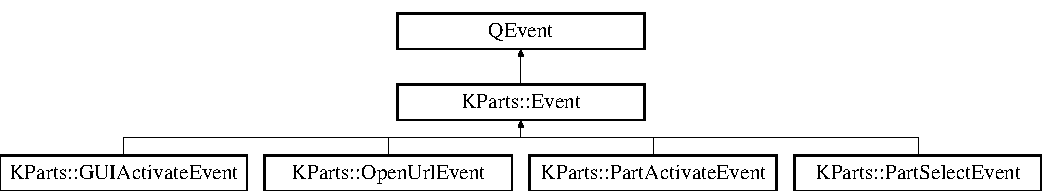
\includegraphics[height=1.707317cm]{classKParts_1_1Event}
\end{center}
\end{figure}
\subsection*{\-Public \-Member \-Functions}
\begin{DoxyCompactItemize}
\item 
\hyperlink{classKParts_1_1Event_af717e4320e2db1ab5973c41381673a4e}{\-Event} (const char $\ast$\hyperlink{classKParts_1_1Event_aefe2f55deef3f5ffc2de198b955fc453}{event\-Name})
\item 
virtual \hyperlink{classKParts_1_1Event_a5e19e5a883bb39c0ea6053170af67081}{$\sim$\-Event} ()
\item 
virtual const char $\ast$ \hyperlink{classKParts_1_1Event_aefe2f55deef3f5ffc2de198b955fc453}{event\-Name} () const 
\end{DoxyCompactItemize}
\subsection*{\-Static \-Public \-Member \-Functions}
\begin{DoxyCompactItemize}
\item 
static bool \hyperlink{classKParts_1_1Event_a825b18534ae37dae24f2a2b326db0629}{test} (const \-Q\-Event $\ast$event)
\item 
static bool \hyperlink{classKParts_1_1Event_a1736144deda3cbb502cb6a9151d3c7cb}{test} (const \-Q\-Event $\ast$event, const char $\ast$name)
\end{DoxyCompactItemize}


\subsection{\-Detailed \-Description}
\-Base class for all \hyperlink{namespaceKParts}{\-K\-Parts} events. 

\-Definition at line 37 of file event.\-h.



\subsection{\-Constructor \& \-Destructor \-Documentation}
\hypertarget{classKParts_1_1Event_af717e4320e2db1ab5973c41381673a4e}{\index{\-K\-Parts\-::\-Event@{\-K\-Parts\-::\-Event}!\-Event@{\-Event}}
\index{\-Event@{\-Event}!KParts::Event@{\-K\-Parts\-::\-Event}}
\subsubsection[{\-Event}]{\setlength{\rightskip}{0pt plus 5cm}{\bf \-K\-Parts\-::\-Event\-::\-Event} (
\begin{DoxyParamCaption}
\item[{const char $\ast$}]{event\-Name}
\end{DoxyParamCaption}
)}}\label{classKParts_1_1Event_af717e4320e2db1ab5973c41381673a4e}
\hypertarget{classKParts_1_1Event_a5e19e5a883bb39c0ea6053170af67081}{\index{\-K\-Parts\-::\-Event@{\-K\-Parts\-::\-Event}!$\sim$\-Event@{$\sim$\-Event}}
\index{$\sim$\-Event@{$\sim$\-Event}!KParts::Event@{\-K\-Parts\-::\-Event}}
\subsubsection[{$\sim$\-Event}]{\setlength{\rightskip}{0pt plus 5cm}virtual {\bf \-K\-Parts\-::\-Event\-::$\sim$\-Event} (
\begin{DoxyParamCaption}
{}
\end{DoxyParamCaption}
)\hspace{0.3cm}{\ttfamily  \mbox{[}virtual\mbox{]}}}}\label{classKParts_1_1Event_a5e19e5a883bb39c0ea6053170af67081}


\subsection{\-Member \-Function \-Documentation}
\hypertarget{classKParts_1_1Event_aefe2f55deef3f5ffc2de198b955fc453}{\index{\-K\-Parts\-::\-Event@{\-K\-Parts\-::\-Event}!event\-Name@{event\-Name}}
\index{event\-Name@{event\-Name}!KParts::Event@{\-K\-Parts\-::\-Event}}
\subsubsection[{event\-Name}]{\setlength{\rightskip}{0pt plus 5cm}virtual const char$\ast$ {\bf \-K\-Parts\-::\-Event\-::event\-Name} (
\begin{DoxyParamCaption}
{}
\end{DoxyParamCaption}
) const\hspace{0.3cm}{\ttfamily  \mbox{[}virtual\mbox{]}}}}\label{classKParts_1_1Event_aefe2f55deef3f5ffc2de198b955fc453}
\hypertarget{classKParts_1_1Event_a825b18534ae37dae24f2a2b326db0629}{\index{\-K\-Parts\-::\-Event@{\-K\-Parts\-::\-Event}!test@{test}}
\index{test@{test}!KParts::Event@{\-K\-Parts\-::\-Event}}
\subsubsection[{test}]{\setlength{\rightskip}{0pt plus 5cm}static bool {\bf \-K\-Parts\-::\-Event\-::test} (
\begin{DoxyParamCaption}
\item[{const \-Q\-Event $\ast$}]{event}
\end{DoxyParamCaption}
)\hspace{0.3cm}{\ttfamily  \mbox{[}static\mbox{]}}}}\label{classKParts_1_1Event_a825b18534ae37dae24f2a2b326db0629}


\-Reimplemented in \hyperlink{classKParts_1_1OpenUrlEvent_aa2c34fa11ddbcbf9828661fe681bcb62}{\-K\-Parts\-::\-Open\-Url\-Event}, \hyperlink{classKParts_1_1PartSelectEvent_acc477c171d8bedc9e9cbcc23cf775024}{\-K\-Parts\-::\-Part\-Select\-Event}, \hyperlink{classKParts_1_1PartActivateEvent_ab2b795f3ff5ed09524e0357ee21cf264}{\-K\-Parts\-::\-Part\-Activate\-Event}, and \hyperlink{classKParts_1_1GUIActivateEvent_a360a35ee2b385c6b615e909e4a885e83}{\-K\-Parts\-::\-G\-U\-I\-Activate\-Event}.

\hypertarget{classKParts_1_1Event_a1736144deda3cbb502cb6a9151d3c7cb}{\index{\-K\-Parts\-::\-Event@{\-K\-Parts\-::\-Event}!test@{test}}
\index{test@{test}!KParts::Event@{\-K\-Parts\-::\-Event}}
\subsubsection[{test}]{\setlength{\rightskip}{0pt plus 5cm}static bool {\bf \-K\-Parts\-::\-Event\-::test} (
\begin{DoxyParamCaption}
\item[{const \-Q\-Event $\ast$}]{event, }
\item[{const char $\ast$}]{name}
\end{DoxyParamCaption}
)\hspace{0.3cm}{\ttfamily  \mbox{[}static\mbox{]}}}}\label{classKParts_1_1Event_a1736144deda3cbb502cb6a9151d3c7cb}


\-The documentation for this class was generated from the following file\-:\begin{DoxyCompactItemize}
\item 
/usr/include/kparts/\hyperlink{event_8h}{event.\-h}\end{DoxyCompactItemize}

\hypertarget{structKParts_1_1ScriptableExtension_1_1Exception}{\section{\-K\-Parts\-:\-:\-Scriptable\-Extension\-:\-:\-Exception \-Struct \-Reference}
\label{structKParts_1_1ScriptableExtension_1_1Exception}\index{\-K\-Parts\-::\-Scriptable\-Extension\-::\-Exception@{\-K\-Parts\-::\-Scriptable\-Extension\-::\-Exception}}
}


{\ttfamily \#include $<$scriptableextension.\-h$>$}

\subsection*{\-Public \-Member \-Functions}
\begin{DoxyCompactItemize}
\item 
\hyperlink{structKParts_1_1ScriptableExtension_1_1Exception_a0e8550fd8417396956f5b7a4fc78768b}{\-Exception} ()
\item 
\hyperlink{structKParts_1_1ScriptableExtension_1_1Exception_ac4c4baf6868b49f539c9f7492ce3515d}{\-Exception} (const \-Q\-String \&msg)
\end{DoxyCompactItemize}
\subsection*{\-Public \-Attributes}
\begin{DoxyCompactItemize}
\item 
\-Q\-String \hyperlink{structKParts_1_1ScriptableExtension_1_1Exception_aa077475854a1ee79ac8905a2e07be407}{message}
\end{DoxyCompactItemize}


\subsection{\-Detailed \-Description}
\-Returned from operations to denote a failure. \-May not be passed in as a parameter, only returned 

\-Definition at line 68 of file scriptableextension.\-h.



\subsection{\-Constructor \& \-Destructor \-Documentation}
\hypertarget{structKParts_1_1ScriptableExtension_1_1Exception_a0e8550fd8417396956f5b7a4fc78768b}{\index{\-K\-Parts\-::\-Scriptable\-Extension\-::\-Exception@{\-K\-Parts\-::\-Scriptable\-Extension\-::\-Exception}!\-Exception@{\-Exception}}
\index{\-Exception@{\-Exception}!KParts::ScriptableExtension::Exception@{\-K\-Parts\-::\-Scriptable\-Extension\-::\-Exception}}
\subsubsection[{\-Exception}]{\setlength{\rightskip}{0pt plus 5cm}{\bf \-K\-Parts\-::\-Scriptable\-Extension\-::\-Exception\-::\-Exception} (
\begin{DoxyParamCaption}
{}
\end{DoxyParamCaption}
)\hspace{0.3cm}{\ttfamily  \mbox{[}inline\mbox{]}}}}\label{structKParts_1_1ScriptableExtension_1_1Exception_a0e8550fd8417396956f5b7a4fc78768b}


\-Definition at line 74 of file scriptableextension.\-h.


\begin{DoxyCode}
{}
\end{DoxyCode}
\hypertarget{structKParts_1_1ScriptableExtension_1_1Exception_ac4c4baf6868b49f539c9f7492ce3515d}{\index{\-K\-Parts\-::\-Scriptable\-Extension\-::\-Exception@{\-K\-Parts\-::\-Scriptable\-Extension\-::\-Exception}!\-Exception@{\-Exception}}
\index{\-Exception@{\-Exception}!KParts::ScriptableExtension::Exception@{\-K\-Parts\-::\-Scriptable\-Extension\-::\-Exception}}
\subsubsection[{\-Exception}]{\setlength{\rightskip}{0pt plus 5cm}{\bf \-K\-Parts\-::\-Scriptable\-Extension\-::\-Exception\-::\-Exception} (
\begin{DoxyParamCaption}
\item[{const \-Q\-String \&}]{msg}
\end{DoxyParamCaption}
)\hspace{0.3cm}{\ttfamily  \mbox{[}inline\mbox{]}}}}\label{structKParts_1_1ScriptableExtension_1_1Exception_ac4c4baf6868b49f539c9f7492ce3515d}


\-Definition at line 75 of file scriptableextension.\-h.


\begin{DoxyCode}
: message(msg) {}
\end{DoxyCode}


\subsection{\-Member \-Data \-Documentation}
\hypertarget{structKParts_1_1ScriptableExtension_1_1Exception_aa077475854a1ee79ac8905a2e07be407}{\index{\-K\-Parts\-::\-Scriptable\-Extension\-::\-Exception@{\-K\-Parts\-::\-Scriptable\-Extension\-::\-Exception}!message@{message}}
\index{message@{message}!KParts::ScriptableExtension::Exception@{\-K\-Parts\-::\-Scriptable\-Extension\-::\-Exception}}
\subsubsection[{message}]{\setlength{\rightskip}{0pt plus 5cm}\-Q\-String {\bf \-K\-Parts\-::\-Scriptable\-Extension\-::\-Exception\-::message}}}\label{structKParts_1_1ScriptableExtension_1_1Exception_aa077475854a1ee79ac8905a2e07be407}
\-Error message returned from the callee. \-This should be assumed to be low-\/level (in particular, it might not be translated) and should only be displayed in low-\/level debugging tools and the like. 

\-Definition at line 72 of file scriptableextension.\-h.



\-The documentation for this struct was generated from the following file\-:\begin{DoxyCompactItemize}
\item 
/usr/include/kparts/\hyperlink{scriptableextension_8h}{scriptableextension.\-h}\end{DoxyCompactItemize}

\hypertarget{classKParts_1_1Factory}{\section{K\+Parts\+:\+:Factory Class Reference}
\label{classKParts_1_1Factory}\index{K\+Parts\+::\+Factory@{K\+Parts\+::\+Factory}}
}


{\ttfamily \#include $<$factory.\+h$>$}

Inheritance diagram for K\+Parts\+:\+:Factory\+:\begin{figure}[H]
\begin{center}
\leavevmode
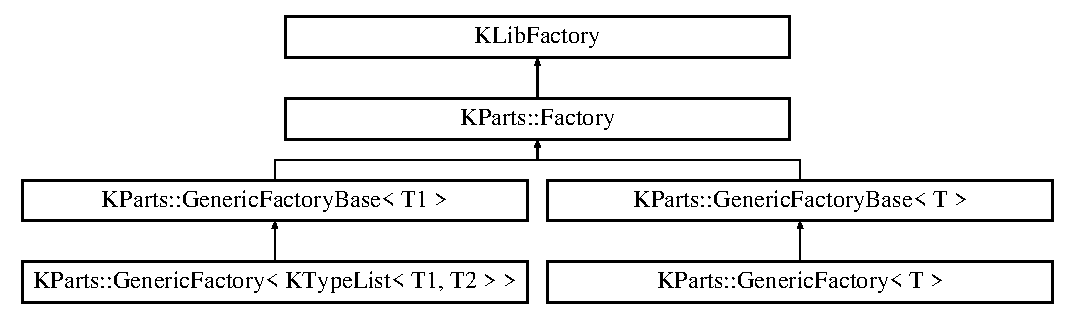
\includegraphics[height=3.835616cm]{classKParts_1_1Factory}
\end{center}
\end{figure}
\subsection*{Public Member Functions}
\begin{DoxyCompactItemize}
\item 
\hyperlink{classKParts_1_1Factory_aa5b7628de21a0b8b32dcd5bd3b3fe3af}{Factory} (Q\+Object $\ast$parent=0)
\item 
virtual \hyperlink{classKParts_1_1Factory_a051bbca3a6feb3a865f7e119112ff813}{$\sim$\+Factory} ()
\item 
\hyperlink{classKParts_1_1Part}{Part} $\ast$ \hyperlink{classKParts_1_1Factory_a41e7c93ddb621d17b7f380a9455ba2a8}{create\+Part} (Q\+Widget $\ast$parent\+Widget=0, Q\+Object $\ast$parent=0, const char $\ast$classname=\char`\"{}K\+Parts\+::\+Part\char`\"{}, const Q\+String\+List \&args=Q\+String\+List())
\item 
virtual K\+Component\+Data \hyperlink{classKParts_1_1Factory_a94c5c244737f0aa7788a1c114bc2acb9}{part\+Component\+Data} ()
\end{DoxyCompactItemize}
\subsection*{Static Public Member Functions}
\begin{DoxyCompactItemize}
\item 
static K\+Component\+Data \hyperlink{classKParts_1_1Factory_a5333c938faf8ecd06a172edb4af5692a}{part\+Component\+Data\+From\+Library} (const Q\+String \&library\+Name)
\end{DoxyCompactItemize}
\subsection*{Protected Member Functions}
\begin{DoxyCompactItemize}
\item 
virtual \hyperlink{classKParts_1_1Part}{Part} $\ast$ \hyperlink{classKParts_1_1Factory_a05e336b747b65776e31db466736570f2}{create\+Part\+Object} (Q\+Widget $\ast$parent\+Widget=0, Q\+Object $\ast$parent=0, const char $\ast$classname=\char`\"{}K\+Parts\+::\+Part\char`\"{}, const Q\+String\+List \&args=Q\+String\+List())=0
\item 
virtual Q\+Object $\ast$ \hyperlink{classKParts_1_1Factory_accec62e4a6f005b82cfad965cbeb1d7b}{create\+Object} (Q\+Object $\ast$parent=0, const char $\ast$classname=\char`\"{}Q\+Object\char`\"{}, const Q\+String\+List \&args=Q\+String\+List())
\end{DoxyCompactItemize}


\subsection{Detailed Description}
A generic factory object to create a \hyperlink{classKParts_1_1Part}{Part}.

\hyperlink{classKParts_1_1Factory}{Factory} is an abstract class. Reimplement the \hyperlink{classKParts_1_1Factory_a05e336b747b65776e31db466736570f2}{create\+Part\+Object()} method to give it functionality.

\begin{DoxySeeAlso}{See Also}
K\+Lib\+Factory. 
\end{DoxySeeAlso}


Definition at line 42 of file factory.\+h.



\subsection{Constructor \& Destructor Documentation}
\hypertarget{classKParts_1_1Factory_aa5b7628de21a0b8b32dcd5bd3b3fe3af}{\index{K\+Parts\+::\+Factory@{K\+Parts\+::\+Factory}!Factory@{Factory}}
\index{Factory@{Factory}!K\+Parts\+::\+Factory@{K\+Parts\+::\+Factory}}
\subsubsection[{Factory}]{\setlength{\rightskip}{0pt plus 5cm}K\+Parts\+::\+Factory\+::\+Factory (
\begin{DoxyParamCaption}
\item[{Q\+Object $\ast$}]{parent = {\ttfamily 0}}
\end{DoxyParamCaption}
)}}\label{classKParts_1_1Factory_aa5b7628de21a0b8b32dcd5bd3b3fe3af}
\hypertarget{classKParts_1_1Factory_a051bbca3a6feb3a865f7e119112ff813}{\index{K\+Parts\+::\+Factory@{K\+Parts\+::\+Factory}!````~Factory@{$\sim$\+Factory}}
\index{````~Factory@{$\sim$\+Factory}!K\+Parts\+::\+Factory@{K\+Parts\+::\+Factory}}
\subsubsection[{$\sim$\+Factory}]{\setlength{\rightskip}{0pt plus 5cm}virtual K\+Parts\+::\+Factory\+::$\sim$\+Factory (
\begin{DoxyParamCaption}
{}
\end{DoxyParamCaption}
)\hspace{0.3cm}{\ttfamily [virtual]}}}\label{classKParts_1_1Factory_a051bbca3a6feb3a865f7e119112ff813}


\subsection{Member Function Documentation}
\hypertarget{classKParts_1_1Factory_accec62e4a6f005b82cfad965cbeb1d7b}{\index{K\+Parts\+::\+Factory@{K\+Parts\+::\+Factory}!create\+Object@{create\+Object}}
\index{create\+Object@{create\+Object}!K\+Parts\+::\+Factory@{K\+Parts\+::\+Factory}}
\subsubsection[{create\+Object}]{\setlength{\rightskip}{0pt plus 5cm}virtual Q\+Object$\ast$ K\+Parts\+::\+Factory\+::create\+Object (
\begin{DoxyParamCaption}
\item[{Q\+Object $\ast$}]{parent = {\ttfamily 0}, }
\item[{const char $\ast$}]{classname = {\ttfamily \char`\"{}QObject\char`\"{}}, }
\item[{const Q\+String\+List \&}]{args = {\ttfamily QStringList()}}
\end{DoxyParamCaption}
)\hspace{0.3cm}{\ttfamily [protected]}, {\ttfamily [virtual]}}}\label{classKParts_1_1Factory_accec62e4a6f005b82cfad965cbeb1d7b}
Reimplemented from K\+Lib\+Factory. Calls \hyperlink{classKParts_1_1Factory_a41e7c93ddb621d17b7f380a9455ba2a8}{create\+Part()} \hypertarget{classKParts_1_1Factory_a41e7c93ddb621d17b7f380a9455ba2a8}{\index{K\+Parts\+::\+Factory@{K\+Parts\+::\+Factory}!create\+Part@{create\+Part}}
\index{create\+Part@{create\+Part}!K\+Parts\+::\+Factory@{K\+Parts\+::\+Factory}}
\subsubsection[{create\+Part}]{\setlength{\rightskip}{0pt plus 5cm}{\bf Part}$\ast$ K\+Parts\+::\+Factory\+::create\+Part (
\begin{DoxyParamCaption}
\item[{Q\+Widget $\ast$}]{parent\+Widget = {\ttfamily 0}, }
\item[{Q\+Object $\ast$}]{parent = {\ttfamily 0}, }
\item[{const char $\ast$}]{classname = {\ttfamily \char`\"{}KParts\+:\+:Part\char`\"{}}, }
\item[{const Q\+String\+List \&}]{args = {\ttfamily QStringList()}}
\end{DoxyParamCaption}
)}}\label{classKParts_1_1Factory_a41e7c93ddb621d17b7f380a9455ba2a8}
Creates a part.

The Q\+String\+List can be used to pass additional arguments to the part. If the part needs additional arguments, it should take them as name=\char`\"{}value\char`\"{} pairs. This is the way additional arguments will get passed to the part from eg. khtml. You can for example emebed the part into H\+T\+M\+L by using the following code\+: 
\begin{DoxyCode}
<\textcolor{keywordtype}{object} type=\textcolor{stringliteral}{"my\_mimetype"} data=\textcolor{stringliteral}{"url\_to\_my\_data"}>
    <param name=\textcolor{stringliteral}{"name1"} value=\textcolor{stringliteral}{"value1"}>
    <param name=\textcolor{stringliteral}{"name2"} value=\textcolor{stringliteral}{"value2"}>
</\textcolor{keywordtype}{object}>
\end{DoxyCode}
 This could result in a call to 
\begin{DoxyCode}
\hyperlink{classKParts_1_1Factory_a41e7c93ddb621d17b7f380a9455ba2a8}{createPart}( parentWidget, parentObject, \textcolor{stringliteral}{"KParts::Part"},
            QStringList(\textcolor{stringliteral}{"name1="}value1\textcolor{stringliteral}{""}, \textcolor{stringliteral}{"name2="}value2\textcolor{stringliteral}{") );}
\end{DoxyCode}


\begin{DoxyReturn}{Returns}
the newly created part.
\end{DoxyReturn}
\hyperlink{classKParts_1_1Factory_a41e7c93ddb621d17b7f380a9455ba2a8}{create\+Part()} automatically emits a signal K\+Lib\+Factory\+::object\+Created to tell the library about its newly created object. This is very important for reference counting, and allows unloading the library automatically once all its objects have been destroyed. \hypertarget{classKParts_1_1Factory_a05e336b747b65776e31db466736570f2}{\index{K\+Parts\+::\+Factory@{K\+Parts\+::\+Factory}!create\+Part\+Object@{create\+Part\+Object}}
\index{create\+Part\+Object@{create\+Part\+Object}!K\+Parts\+::\+Factory@{K\+Parts\+::\+Factory}}
\subsubsection[{create\+Part\+Object}]{\setlength{\rightskip}{0pt plus 5cm}virtual {\bf Part}$\ast$ K\+Parts\+::\+Factory\+::create\+Part\+Object (
\begin{DoxyParamCaption}
\item[{Q\+Widget $\ast$}]{parent\+Widget = {\ttfamily 0}, }
\item[{Q\+Object $\ast$}]{parent = {\ttfamily 0}, }
\item[{const char $\ast$}]{classname = {\ttfamily \char`\"{}KParts\+:\+:Part\char`\"{}}, }
\item[{const Q\+String\+List \&}]{args = {\ttfamily QStringList()}}
\end{DoxyParamCaption}
)\hspace{0.3cm}{\ttfamily [protected]}, {\ttfamily [pure virtual]}}}\label{classKParts_1_1Factory_a05e336b747b65776e31db466736570f2}
Reimplement this method in your implementation to create the \hyperlink{classKParts_1_1Part}{Part}.

The Q\+String\+List can be used to pass additional arguments to the part. If the part needs additional arguments, it should take them as name=\char`\"{}value\char`\"{} pairs. This is the way additional arguments will get passed to the part from eg. khtml. You can for example emebed the part into H\+T\+M\+L by using the following code\+: 
\begin{DoxyCode}
<\textcolor{keywordtype}{object} type=\textcolor{stringliteral}{"my\_mimetype"} data=\textcolor{stringliteral}{"url\_to\_my\_data"}>
    <param name=\textcolor{stringliteral}{"name1"} value=\textcolor{stringliteral}{"value1"}>
    <param name=\textcolor{stringliteral}{"name2"} value=\textcolor{stringliteral}{"value2"}>
</\textcolor{keywordtype}{object}>
\end{DoxyCode}
 This could result in a call to 
\begin{DoxyCode}
\hyperlink{classKParts_1_1Factory_a41e7c93ddb621d17b7f380a9455ba2a8}{createPart}( parentWidget, parentObject, \textcolor{stringliteral}{"KParts::Part"},
            QStringList(\textcolor{stringliteral}{"name1="}value1\textcolor{stringliteral}{""}, \textcolor{stringliteral}{"name2="}value2\textcolor{stringliteral}{") );}
\end{DoxyCode}


\begin{DoxyReturn}{Returns}
the newly created part. 
\end{DoxyReturn}


Implemented in \hyperlink{classKParts_1_1GenericFactory_3_01KTypeList_3_01T1_00_01T2_01_4_01_4_aa3e8c27c10a09306951a2e63159a3d56}{K\+Parts\+::\+Generic\+Factory$<$ K\+Type\+List$<$ T1, T2 $>$ $>$}, and \hyperlink{classKParts_1_1GenericFactory_ac80d722fb2433018dfea04f0f6b89f74}{K\+Parts\+::\+Generic\+Factory$<$ T $>$}.

\hypertarget{classKParts_1_1Factory_a94c5c244737f0aa7788a1c114bc2acb9}{\index{K\+Parts\+::\+Factory@{K\+Parts\+::\+Factory}!part\+Component\+Data@{part\+Component\+Data}}
\index{part\+Component\+Data@{part\+Component\+Data}!K\+Parts\+::\+Factory@{K\+Parts\+::\+Factory}}
\subsubsection[{part\+Component\+Data}]{\setlength{\rightskip}{0pt plus 5cm}virtual K\+Component\+Data K\+Parts\+::\+Factory\+::part\+Component\+Data (
\begin{DoxyParamCaption}
{}
\end{DoxyParamCaption}
)\hspace{0.3cm}{\ttfamily [virtual]}}}\label{classKParts_1_1Factory_a94c5c244737f0aa7788a1c114bc2acb9}
If you have a part contained in a shared library you might want to query for meta-\/information like the about-\/data, or the K\+Component\+Data in general. If the part is exported using \hyperlink{classKParts_1_1GenericFactory}{K\+Parts\+::\+Generic\+Factory} then this method will return the instance that belongs to the part without the need to instantiate the part component. 

Reimplemented in \hyperlink{classKParts_1_1GenericFactoryBase_a0b1d32c7adf2255890bdd3898757feae}{K\+Parts\+::\+Generic\+Factory\+Base$<$ T $>$}, and \hyperlink{classKParts_1_1GenericFactoryBase_a0b1d32c7adf2255890bdd3898757feae}{K\+Parts\+::\+Generic\+Factory\+Base$<$ T1 $>$}.

\hypertarget{classKParts_1_1Factory_a5333c938faf8ecd06a172edb4af5692a}{\index{K\+Parts\+::\+Factory@{K\+Parts\+::\+Factory}!part\+Component\+Data\+From\+Library@{part\+Component\+Data\+From\+Library}}
\index{part\+Component\+Data\+From\+Library@{part\+Component\+Data\+From\+Library}!K\+Parts\+::\+Factory@{K\+Parts\+::\+Factory}}
\subsubsection[{part\+Component\+Data\+From\+Library}]{\setlength{\rightskip}{0pt plus 5cm}static K\+Component\+Data K\+Parts\+::\+Factory\+::part\+Component\+Data\+From\+Library (
\begin{DoxyParamCaption}
\item[{const Q\+String \&}]{library\+Name}
\end{DoxyParamCaption}
)\hspace{0.3cm}{\ttfamily [static]}}}\label{classKParts_1_1Factory_a5333c938faf8ecd06a172edb4af5692a}
A convenience method for part\+Component\+Data that takes care of retrieving the factory for a given library name and calling part\+Component\+Data on it.


\begin{DoxyParams}{Parameters}
{\em library\+Name} & name of the library to query the instance from \\
\hline
\end{DoxyParams}


The documentation for this class was generated from the following file\+:\begin{DoxyCompactItemize}
\item 
/usr/include/kparts/\hyperlink{factory_8h}{factory.\+h}\end{DoxyCompactItemize}

\hypertarget{classKParts_1_1FileInfoExtension}{\section{K\+Parts\+:\+:File\+Info\+Extension Class Reference}
\label{classKParts_1_1FileInfoExtension}\index{K\+Parts\+::\+File\+Info\+Extension@{K\+Parts\+::\+File\+Info\+Extension}}
}


an extension for obtaining file information from the part.  




{\ttfamily \#include $<$fileinfoextension.\+h$>$}

Inheritance diagram for K\+Parts\+:\+:File\+Info\+Extension\+:\begin{figure}[H]
\begin{center}
\leavevmode
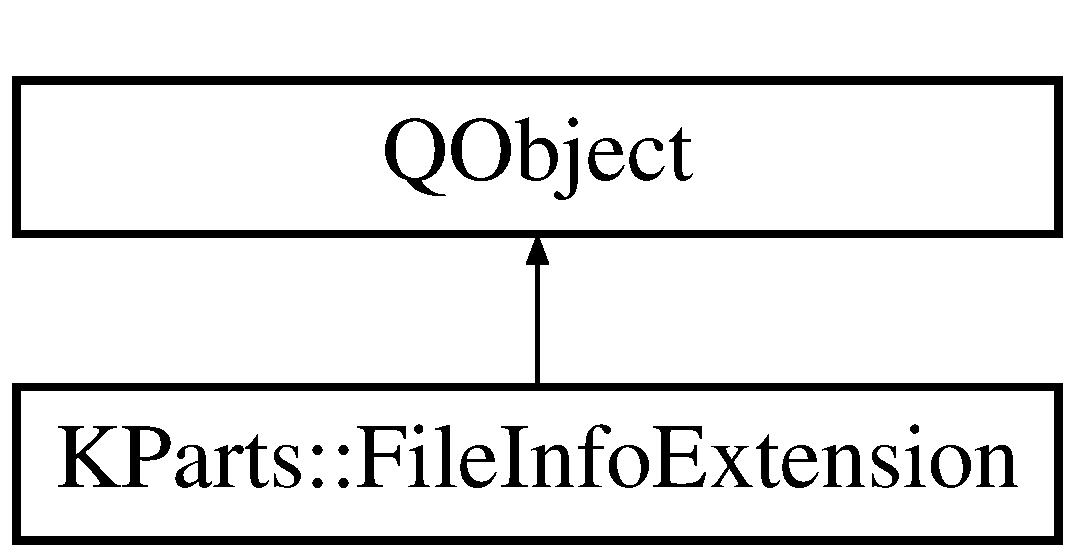
\includegraphics[height=2.000000cm]{classKParts_1_1FileInfoExtension}
\end{center}
\end{figure}
\subsection*{Public Types}
\begin{DoxyCompactItemize}
\item 
enum \hyperlink{classKParts_1_1FileInfoExtension_a9bc830a53b0005013082984a2bbd5639}{Query\+Mode} \{ \hyperlink{classKParts_1_1FileInfoExtension_a9bc830a53b0005013082984a2bbd5639af7f7b524610ed47f67081fee1a37a604}{None} = 0x00, 
\hyperlink{classKParts_1_1FileInfoExtension_a9bc830a53b0005013082984a2bbd5639a553b2481b4b7b99d8f839eed303177d8}{All\+Items} = 0x01, 
\hyperlink{classKParts_1_1FileInfoExtension_a9bc830a53b0005013082984a2bbd5639aaa07fd2649d0deb94a819b29cddbe32e}{Selected\+Items} = 0x02
 \}
\end{DoxyCompactItemize}
\subsection*{Public Member Functions}
\begin{DoxyCompactItemize}
\item 
\hyperlink{classKParts_1_1FileInfoExtension_ab7f24a4cbfcabe40422b26fa2ee562b7}{File\+Info\+Extension} (\hyperlink{classKParts_1_1ReadOnlyPart}{K\+Parts\+::\+Read\+Only\+Part} $\ast$parent)
\item 
virtual \hyperlink{classKParts_1_1FileInfoExtension_aefda4c72d82131c2dd8cc2e69d157a90}{$\sim$\+File\+Info\+Extension} ()
\item 
virtual bool \hyperlink{classKParts_1_1FileInfoExtension_a4774dbd7c4debae026e6103ba0b4ffd5}{has\+Selection} () const 
\item 
virtual Query\+Modes \hyperlink{classKParts_1_1FileInfoExtension_aa07ffdbb4c8ecc67d75836d48cb33250}{supported\+Query\+Modes} () const 
\item 
virtual K\+File\+Item\+List \hyperlink{classKParts_1_1FileInfoExtension_addac1579dcbc21c5fcceecda6f5cb532}{query\+For} (\hyperlink{classKParts_1_1FileInfoExtension_a9bc830a53b0005013082984a2bbd5639}{Query\+Mode} mode) const =0
\end{DoxyCompactItemize}
\subsection*{Static Public Member Functions}
\begin{DoxyCompactItemize}
\item 
static \hyperlink{classKParts_1_1FileInfoExtension}{File\+Info\+Extension} $\ast$ \hyperlink{classKParts_1_1FileInfoExtension_a1c137505684c839e52edff6b3592a264}{child\+Object} (Q\+Object $\ast$obj)
\end{DoxyCompactItemize}


\subsection{Detailed Description}
an extension for obtaining file information from the part. 

This extension provides information about file and directory resources that are present in the part the implements it.

The main purpose of for this extension is to provide information about files and directories located on remote servers so that download managers such as kget can easily retrieve these resources.

\begin{DoxySince}{Since}
4.\+6 
\end{DoxySince}


Definition at line 48 of file fileinfoextension.\+h.



\subsection{Member Enumeration Documentation}
\hypertarget{classKParts_1_1FileInfoExtension_a9bc830a53b0005013082984a2bbd5639}{\index{K\+Parts\+::\+File\+Info\+Extension@{K\+Parts\+::\+File\+Info\+Extension}!Query\+Mode@{Query\+Mode}}
\index{Query\+Mode@{Query\+Mode}!K\+Parts\+::\+File\+Info\+Extension@{K\+Parts\+::\+File\+Info\+Extension}}
\subsubsection[{Query\+Mode}]{\setlength{\rightskip}{0pt plus 5cm}enum {\bf K\+Parts\+::\+File\+Info\+Extension\+::\+Query\+Mode}}}\label{classKParts_1_1FileInfoExtension_a9bc830a53b0005013082984a2bbd5639}
Supported file information retrieval modes. \begin{Desc}
\item[Enumerator]\par
\begin{description}
\index{None@{None}!K\+Parts\+::\+File\+Info\+Extension@{K\+Parts\+::\+File\+Info\+Extension}}\index{K\+Parts\+::\+File\+Info\+Extension@{K\+Parts\+::\+File\+Info\+Extension}!None@{None}}\item[{\em 
\hypertarget{classKParts_1_1FileInfoExtension_a9bc830a53b0005013082984a2bbd5639af7f7b524610ed47f67081fee1a37a604}{None}\label{classKParts_1_1FileInfoExtension_a9bc830a53b0005013082984a2bbd5639af7f7b524610ed47f67081fee1a37a604}
}]Querying for file information is N\+O\+T possible \index{All\+Items@{All\+Items}!K\+Parts\+::\+File\+Info\+Extension@{K\+Parts\+::\+File\+Info\+Extension}}\index{K\+Parts\+::\+File\+Info\+Extension@{K\+Parts\+::\+File\+Info\+Extension}!All\+Items@{All\+Items}}\item[{\em 
\hypertarget{classKParts_1_1FileInfoExtension_a9bc830a53b0005013082984a2bbd5639a553b2481b4b7b99d8f839eed303177d8}{All\+Items}\label{classKParts_1_1FileInfoExtension_a9bc830a53b0005013082984a2bbd5639a553b2481b4b7b99d8f839eed303177d8}
}]Retrieve or can retrieve file information for all items. \index{Selected\+Items@{Selected\+Items}!K\+Parts\+::\+File\+Info\+Extension@{K\+Parts\+::\+File\+Info\+Extension}}\index{K\+Parts\+::\+File\+Info\+Extension@{K\+Parts\+::\+File\+Info\+Extension}!Selected\+Items@{Selected\+Items}}\item[{\em 
\hypertarget{classKParts_1_1FileInfoExtension_a9bc830a53b0005013082984a2bbd5639aaa07fd2649d0deb94a819b29cddbe32e}{Selected\+Items}\label{classKParts_1_1FileInfoExtension_a9bc830a53b0005013082984a2bbd5639aaa07fd2649d0deb94a819b29cddbe32e}
}]Retrieve or can retrieve file information for selected items. \end{description}
\end{Desc}


Definition at line 57 of file fileinfoextension.\+h.


\begin{DoxyCode}
57                     \{
58         \hyperlink{classKParts_1_1FileInfoExtension_a9bc830a53b0005013082984a2bbd5639af7f7b524610ed47f67081fee1a37a604}{None} = 0x00,              
59         \hyperlink{classKParts_1_1FileInfoExtension_a9bc830a53b0005013082984a2bbd5639a553b2481b4b7b99d8f839eed303177d8}{AllItems} = 0x01,          
60         \hyperlink{classKParts_1_1FileInfoExtension_a9bc830a53b0005013082984a2bbd5639aaa07fd2649d0deb94a819b29cddbe32e}{SelectedItems} = 0x02      
61     \};
\end{DoxyCode}


\subsection{Constructor \& Destructor Documentation}
\hypertarget{classKParts_1_1FileInfoExtension_ab7f24a4cbfcabe40422b26fa2ee562b7}{\index{K\+Parts\+::\+File\+Info\+Extension@{K\+Parts\+::\+File\+Info\+Extension}!File\+Info\+Extension@{File\+Info\+Extension}}
\index{File\+Info\+Extension@{File\+Info\+Extension}!K\+Parts\+::\+File\+Info\+Extension@{K\+Parts\+::\+File\+Info\+Extension}}
\subsubsection[{File\+Info\+Extension}]{\setlength{\rightskip}{0pt plus 5cm}K\+Parts\+::\+File\+Info\+Extension\+::\+File\+Info\+Extension (
\begin{DoxyParamCaption}
\item[{{\bf K\+Parts\+::\+Read\+Only\+Part} $\ast$}]{parent}
\end{DoxyParamCaption}
)}}\label{classKParts_1_1FileInfoExtension_ab7f24a4cbfcabe40422b26fa2ee562b7}
Constructor \hypertarget{classKParts_1_1FileInfoExtension_aefda4c72d82131c2dd8cc2e69d157a90}{\index{K\+Parts\+::\+File\+Info\+Extension@{K\+Parts\+::\+File\+Info\+Extension}!````~File\+Info\+Extension@{$\sim$\+File\+Info\+Extension}}
\index{````~File\+Info\+Extension@{$\sim$\+File\+Info\+Extension}!K\+Parts\+::\+File\+Info\+Extension@{K\+Parts\+::\+File\+Info\+Extension}}
\subsubsection[{$\sim$\+File\+Info\+Extension}]{\setlength{\rightskip}{0pt plus 5cm}virtual K\+Parts\+::\+File\+Info\+Extension\+::$\sim$\+File\+Info\+Extension (
\begin{DoxyParamCaption}
{}
\end{DoxyParamCaption}
)\hspace{0.3cm}{\ttfamily [virtual]}}}\label{classKParts_1_1FileInfoExtension_aefda4c72d82131c2dd8cc2e69d157a90}
Destructor 

\subsection{Member Function Documentation}
\hypertarget{classKParts_1_1FileInfoExtension_a1c137505684c839e52edff6b3592a264}{\index{K\+Parts\+::\+File\+Info\+Extension@{K\+Parts\+::\+File\+Info\+Extension}!child\+Object@{child\+Object}}
\index{child\+Object@{child\+Object}!K\+Parts\+::\+File\+Info\+Extension@{K\+Parts\+::\+File\+Info\+Extension}}
\subsubsection[{child\+Object}]{\setlength{\rightskip}{0pt plus 5cm}static {\bf File\+Info\+Extension}$\ast$ K\+Parts\+::\+File\+Info\+Extension\+::child\+Object (
\begin{DoxyParamCaption}
\item[{Q\+Object $\ast$}]{obj}
\end{DoxyParamCaption}
)\hspace{0.3cm}{\ttfamily [static]}}}\label{classKParts_1_1FileInfoExtension_a1c137505684c839e52edff6b3592a264}
Queries {\ttfamily obj} for a child object which inherits from this class. \hypertarget{classKParts_1_1FileInfoExtension_a4774dbd7c4debae026e6103ba0b4ffd5}{\index{K\+Parts\+::\+File\+Info\+Extension@{K\+Parts\+::\+File\+Info\+Extension}!has\+Selection@{has\+Selection}}
\index{has\+Selection@{has\+Selection}!K\+Parts\+::\+File\+Info\+Extension@{K\+Parts\+::\+File\+Info\+Extension}}
\subsubsection[{has\+Selection}]{\setlength{\rightskip}{0pt plus 5cm}virtual bool K\+Parts\+::\+File\+Info\+Extension\+::has\+Selection (
\begin{DoxyParamCaption}
{}
\end{DoxyParamCaption}
) const\hspace{0.3cm}{\ttfamily [virtual]}}}\label{classKParts_1_1FileInfoExtension_a4774dbd7c4debae026e6103ba0b4ffd5}
Returns true if any of the items in the current view of the part that implements this extension are selected.

By default this function returns false. \hypertarget{classKParts_1_1FileInfoExtension_addac1579dcbc21c5fcceecda6f5cb532}{\index{K\+Parts\+::\+File\+Info\+Extension@{K\+Parts\+::\+File\+Info\+Extension}!query\+For@{query\+For}}
\index{query\+For@{query\+For}!K\+Parts\+::\+File\+Info\+Extension@{K\+Parts\+::\+File\+Info\+Extension}}
\subsubsection[{query\+For}]{\setlength{\rightskip}{0pt plus 5cm}virtual K\+File\+Item\+List K\+Parts\+::\+File\+Info\+Extension\+::query\+For (
\begin{DoxyParamCaption}
\item[{{\bf Query\+Mode}}]{mode}
\end{DoxyParamCaption}
) const\hspace{0.3cm}{\ttfamily [pure virtual]}}}\label{classKParts_1_1FileInfoExtension_addac1579dcbc21c5fcceecda6f5cb532}
Returns a information for files that match the specified query {\ttfamily mode}.

If the mode specified by {\ttfamily mode} is not supported or cannot be handled, then an empty list is returned. \hypertarget{classKParts_1_1FileInfoExtension_aa07ffdbb4c8ecc67d75836d48cb33250}{\index{K\+Parts\+::\+File\+Info\+Extension@{K\+Parts\+::\+File\+Info\+Extension}!supported\+Query\+Modes@{supported\+Query\+Modes}}
\index{supported\+Query\+Modes@{supported\+Query\+Modes}!K\+Parts\+::\+File\+Info\+Extension@{K\+Parts\+::\+File\+Info\+Extension}}
\subsubsection[{supported\+Query\+Modes}]{\setlength{\rightskip}{0pt plus 5cm}virtual Query\+Modes K\+Parts\+::\+File\+Info\+Extension\+::supported\+Query\+Modes (
\begin{DoxyParamCaption}
{}
\end{DoxyParamCaption}
) const\hspace{0.3cm}{\ttfamily [virtual]}}}\label{classKParts_1_1FileInfoExtension_aa07ffdbb4c8ecc67d75836d48cb33250}
Returns the file information retrieve modes supported by the part that implements this extension.

By default this function returns None. 

The documentation for this class was generated from the following file\+:\begin{DoxyCompactItemize}
\item 
/usr/include/kparts/\hyperlink{fileinfoextension_8h}{fileinfoextension.\+h}\end{DoxyCompactItemize}

\hypertarget{structKParts_1_1ScriptableExtension_1_1FunctionRef}{\section{\-K\-Parts\-:\-:\-Scriptable\-Extension\-:\-:\-Function\-Ref \-Struct \-Reference}
\label{structKParts_1_1ScriptableExtension_1_1FunctionRef}\index{\-K\-Parts\-::\-Scriptable\-Extension\-::\-Function\-Ref@{\-K\-Parts\-::\-Scriptable\-Extension\-::\-Function\-Ref}}
}


{\ttfamily \#include $<$scriptableextension.\-h$>$}

\subsection*{\-Public \-Member \-Functions}
\begin{DoxyCompactItemize}
\item 
\hyperlink{structKParts_1_1ScriptableExtension_1_1FunctionRef_a86b2595b7fdf73a3bc128b295792f3da}{\-Function\-Ref} ()
\item 
\hyperlink{structKParts_1_1ScriptableExtension_1_1FunctionRef_a0349d019315c9ec43aa75c91c184b500}{\-Function\-Ref} (const \hyperlink{structKParts_1_1ScriptableExtension_1_1Object}{\-Object} \&b, const \-Q\-String \&f)
\item 
bool \hyperlink{structKParts_1_1ScriptableExtension_1_1FunctionRef_a97f50a9c52fb32ae83cfc07768866c9d}{operator==} (const \hyperlink{structKParts_1_1ScriptableExtension_1_1FunctionRef}{\-Function\-Ref} \&other) const 
\end{DoxyCompactItemize}
\subsection*{\-Public \-Attributes}
\begin{DoxyCompactItemize}
\item 
\hyperlink{structKParts_1_1ScriptableExtension_1_1Object}{\-Object} \hyperlink{structKParts_1_1ScriptableExtension_1_1FunctionRef_aefa54e151818239bce80641973c79e18}{base}
\item 
\-Q\-String \hyperlink{structKParts_1_1ScriptableExtension_1_1FunctionRef_a1e3cffbdcfde393b9ff6243080edbbd4}{field}
\end{DoxyCompactItemize}


\subsection{\-Detailed \-Description}
\-Function references are a pair of an object and a field in it. \-Essentially, if you have a base.\-field(something) call, the 'base' needs to be passed as the 'this' to the function, and these references can be used to resolve that. 

\-Definition at line 104 of file scriptableextension.\-h.



\subsection{\-Constructor \& \-Destructor \-Documentation}
\hypertarget{structKParts_1_1ScriptableExtension_1_1FunctionRef_a86b2595b7fdf73a3bc128b295792f3da}{\index{\-K\-Parts\-::\-Scriptable\-Extension\-::\-Function\-Ref@{\-K\-Parts\-::\-Scriptable\-Extension\-::\-Function\-Ref}!\-Function\-Ref@{\-Function\-Ref}}
\index{\-Function\-Ref@{\-Function\-Ref}!KParts::ScriptableExtension::FunctionRef@{\-K\-Parts\-::\-Scriptable\-Extension\-::\-Function\-Ref}}
\subsubsection[{\-Function\-Ref}]{\setlength{\rightskip}{0pt plus 5cm}{\bf \-K\-Parts\-::\-Scriptable\-Extension\-::\-Function\-Ref\-::\-Function\-Ref} (
\begin{DoxyParamCaption}
{}
\end{DoxyParamCaption}
)\hspace{0.3cm}{\ttfamily  \mbox{[}inline\mbox{]}}}}\label{structKParts_1_1ScriptableExtension_1_1FunctionRef_a86b2595b7fdf73a3bc128b295792f3da}


\-Definition at line 108 of file scriptableextension.\-h.


\begin{DoxyCode}
{}
\end{DoxyCode}
\hypertarget{structKParts_1_1ScriptableExtension_1_1FunctionRef_a0349d019315c9ec43aa75c91c184b500}{\index{\-K\-Parts\-::\-Scriptable\-Extension\-::\-Function\-Ref@{\-K\-Parts\-::\-Scriptable\-Extension\-::\-Function\-Ref}!\-Function\-Ref@{\-Function\-Ref}}
\index{\-Function\-Ref@{\-Function\-Ref}!KParts::ScriptableExtension::FunctionRef@{\-K\-Parts\-::\-Scriptable\-Extension\-::\-Function\-Ref}}
\subsubsection[{\-Function\-Ref}]{\setlength{\rightskip}{0pt plus 5cm}{\bf \-K\-Parts\-::\-Scriptable\-Extension\-::\-Function\-Ref\-::\-Function\-Ref} (
\begin{DoxyParamCaption}
\item[{const {\bf \-Object} \&}]{b, }
\item[{const \-Q\-String \&}]{f}
\end{DoxyParamCaption}
)\hspace{0.3cm}{\ttfamily  \mbox{[}inline\mbox{]}}}}\label{structKParts_1_1ScriptableExtension_1_1FunctionRef_a0349d019315c9ec43aa75c91c184b500}


\-Definition at line 109 of file scriptableextension.\-h.


\begin{DoxyCode}
: base(b), field(f) {}
\end{DoxyCode}


\subsection{\-Member \-Function \-Documentation}
\hypertarget{structKParts_1_1ScriptableExtension_1_1FunctionRef_a97f50a9c52fb32ae83cfc07768866c9d}{\index{\-K\-Parts\-::\-Scriptable\-Extension\-::\-Function\-Ref@{\-K\-Parts\-::\-Scriptable\-Extension\-::\-Function\-Ref}!operator==@{operator==}}
\index{operator==@{operator==}!KParts::ScriptableExtension::FunctionRef@{\-K\-Parts\-::\-Scriptable\-Extension\-::\-Function\-Ref}}
\subsubsection[{operator==}]{\setlength{\rightskip}{0pt plus 5cm}bool \-K\-Parts\-::\-Scriptable\-Extension\-::\-Function\-Ref\-::operator== (
\begin{DoxyParamCaption}
\item[{const {\bf \-Function\-Ref} \&}]{other}
\end{DoxyParamCaption}
) const\hspace{0.3cm}{\ttfamily  \mbox{[}inline\mbox{]}}}}\label{structKParts_1_1ScriptableExtension_1_1FunctionRef_a97f50a9c52fb32ae83cfc07768866c9d}


\-Definition at line 110 of file scriptableextension.\-h.


\begin{DoxyCode}
{ return base == other.base && field == other.field; }
\end{DoxyCode}


\subsection{\-Member \-Data \-Documentation}
\hypertarget{structKParts_1_1ScriptableExtension_1_1FunctionRef_aefa54e151818239bce80641973c79e18}{\index{\-K\-Parts\-::\-Scriptable\-Extension\-::\-Function\-Ref@{\-K\-Parts\-::\-Scriptable\-Extension\-::\-Function\-Ref}!base@{base}}
\index{base@{base}!KParts::ScriptableExtension::FunctionRef@{\-K\-Parts\-::\-Scriptable\-Extension\-::\-Function\-Ref}}
\subsubsection[{base}]{\setlength{\rightskip}{0pt plus 5cm}{\bf \-Object} {\bf \-K\-Parts\-::\-Scriptable\-Extension\-::\-Function\-Ref\-::base}}}\label{structKParts_1_1ScriptableExtension_1_1FunctionRef_aefa54e151818239bce80641973c79e18}


\-Definition at line 105 of file scriptableextension.\-h.

\hypertarget{structKParts_1_1ScriptableExtension_1_1FunctionRef_a1e3cffbdcfde393b9ff6243080edbbd4}{\index{\-K\-Parts\-::\-Scriptable\-Extension\-::\-Function\-Ref@{\-K\-Parts\-::\-Scriptable\-Extension\-::\-Function\-Ref}!field@{field}}
\index{field@{field}!KParts::ScriptableExtension::FunctionRef@{\-K\-Parts\-::\-Scriptable\-Extension\-::\-Function\-Ref}}
\subsubsection[{field}]{\setlength{\rightskip}{0pt plus 5cm}\-Q\-String {\bf \-K\-Parts\-::\-Scriptable\-Extension\-::\-Function\-Ref\-::field}}}\label{structKParts_1_1ScriptableExtension_1_1FunctionRef_a1e3cffbdcfde393b9ff6243080edbbd4}


\-Definition at line 106 of file scriptableextension.\-h.



\-The documentation for this struct was generated from the following file\-:\begin{DoxyCompactItemize}
\item 
/usr/include/kparts/\hyperlink{scriptableextension_8h}{scriptableextension.\-h}\end{DoxyCompactItemize}

\hypertarget{classKParts_1_1GenericFactory}{\section{\-K\-Parts\-:\-:\-Generic\-Factory$<$ \-T $>$ \-Class \-Template \-Reference}
\label{classKParts_1_1GenericFactory}\index{\-K\-Parts\-::\-Generic\-Factory$<$ T $>$@{\-K\-Parts\-::\-Generic\-Factory$<$ T $>$}}
}


{\ttfamily \#include $<$genericfactory.\-h$>$}

\-Inheritance diagram for \-K\-Parts\-:\-:\-Generic\-Factory$<$ \-T $>$\-:\begin{figure}[H]
\begin{center}
\leavevmode
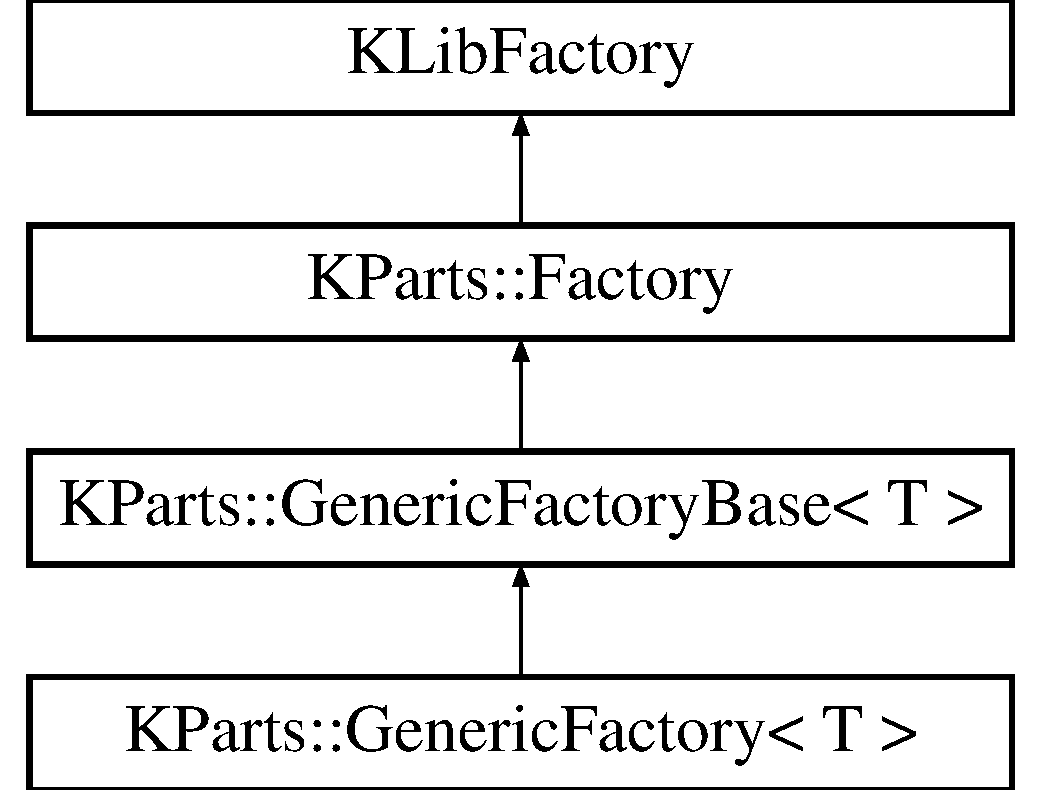
\includegraphics[height=3.000000cm]{classKParts_1_1GenericFactory}
\end{center}
\end{figure}
\subsection*{\-Public \-Member \-Functions}
\begin{DoxyCompactItemize}
\item 
\hyperlink{classKParts_1_1GenericFactory_aef00baf603a775a324f84fb30ba5a0f4}{\-Generic\-Factory} ()
\item 
virtual \hyperlink{classKParts_1_1Part}{\-K\-Parts\-::\-Part} $\ast$ \hyperlink{classKParts_1_1GenericFactory_ac80d722fb2433018dfea04f0f6b89f74}{create\-Part\-Object} (\-Q\-Widget $\ast$parent\-Widget, \-Q\-Object $\ast$parent, const char $\ast$class\-Name, const \-Q\-String\-List \&args)
\end{DoxyCompactItemize}


\subsection{\-Detailed \-Description}
\subsubsection*{template$<$class T$>$class K\-Parts\-::\-Generic\-Factory$<$ T $>$}

\-A template for a \hyperlink{classKParts_1_1Factory}{\-K\-Parts\-::\-Factory} implementation. \-It implements the pure virtual create\-Part\-Object method by instantiating the template argument when requested through the class\-Name field. \-In addition it is a container for a part's \-K\-Component\-Data object, by providing a static \-K\-Component\-Data \hyperlink{classKParts_1_1GenericFactoryBase_ad4a0ca70dec2fe8f4e0d4293e17eb776}{component\-Data()} method.

\-The template argument has to inherit from \hyperlink{classKParts_1_1Part}{\-K\-Parts\-::\-Part} and has to implement two methods\-: 1) \-There needs to be a public constructor with the following signature\-: \-My\-Part( Q\-Widget $\ast$parent\-Widget, Q\-Object $\ast$parent, const Q\-String\-List\& args )

2) \-It needs to provide one static method to create a \-K\-About\-Data object per request, holding information about the component's name, its authors, license, etc. \-The signature of that static method has to be \-K\-About\-Data $\ast$create\-About\-Data()

\-The template will take care of memory management of the \-K\-Component\-Data and the \-K\-About\-Data object, meaning ownership of what create\-About\-Data returns is passed to the caller (this template) .

\-For advanced use you can also inherit from the template and re-\/implement additionally the virtual \-K\-Component\-Data \hyperlink{classKParts_1_1GenericFactoryBase_ae90ec2009529241553290269f3108134}{create\-Component\-Data()} method, for example in case you want to extend the paths of your instance's \-K\-Standard\-Dirs object.

\-If a \hyperlink{classKParts_1_1ReadOnlyPart}{\-K\-Parts\-::\-Read\-Only\-Part} is requested through this factory and the template argument implements a \hyperlink{classKParts_1_1ReadWritePart}{\-K\-Parts\-::\-Read\-Write\-Part} then set\-Read\-Write( false ) will automatically be called in create\-Part\-Object.

\-Use the factory through the \-K\-\_\-\-E\-X\-P\-O\-R\-T\-\_\-\-C\-O\-M\-P\-O\-N\-E\-N\-T\-\_\-\-F\-A\-C\-T\-O\-R\-Y macro, like that\-: 
\begin{DoxyCode}
 typedef KParts::GenericFactory&lt;YourKPart&gt; YourKPartFactory;
 K_EXPORT_COMPONENT_FACTORY( yourlibrary, YourKPartFactory )
\end{DoxyCode}
 yourlibrary is the library name that you compiled your \-K\-Part into. 

\-Definition at line 110 of file genericfactory.\-h.



\subsection{\-Constructor \& \-Destructor \-Documentation}
\hypertarget{classKParts_1_1GenericFactory_aef00baf603a775a324f84fb30ba5a0f4}{\index{\-K\-Parts\-::\-Generic\-Factory@{\-K\-Parts\-::\-Generic\-Factory}!\-Generic\-Factory@{\-Generic\-Factory}}
\index{\-Generic\-Factory@{\-Generic\-Factory}!KParts::GenericFactory@{\-K\-Parts\-::\-Generic\-Factory}}
\subsubsection[{\-Generic\-Factory}]{\setlength{\rightskip}{0pt plus 5cm}template$<$class T $>$ {\bf \-K\-Parts\-::\-Generic\-Factory}$<$ \-T $>$\-::{\bf \-Generic\-Factory} (
\begin{DoxyParamCaption}
{}
\end{DoxyParamCaption}
)\hspace{0.3cm}{\ttfamily  \mbox{[}inline\mbox{]}}}}\label{classKParts_1_1GenericFactory_aef00baf603a775a324f84fb30ba5a0f4}


\-Definition at line 113 of file genericfactory.\-h.


\begin{DoxyCode}
{ }
\end{DoxyCode}


\subsection{\-Member \-Function \-Documentation}
\hypertarget{classKParts_1_1GenericFactory_ac80d722fb2433018dfea04f0f6b89f74}{\index{\-K\-Parts\-::\-Generic\-Factory@{\-K\-Parts\-::\-Generic\-Factory}!create\-Part\-Object@{create\-Part\-Object}}
\index{create\-Part\-Object@{create\-Part\-Object}!KParts::GenericFactory@{\-K\-Parts\-::\-Generic\-Factory}}
\subsubsection[{create\-Part\-Object}]{\setlength{\rightskip}{0pt plus 5cm}template$<$class T $>$ virtual {\bf \-K\-Parts\-::\-Part}$\ast$ {\bf \-K\-Parts\-::\-Generic\-Factory}$<$ \-T $>$\-::{\bf create\-Part\-Object} (
\begin{DoxyParamCaption}
\item[{\-Q\-Widget $\ast$}]{parent\-Widget, }
\item[{\-Q\-Object $\ast$}]{parent, }
\item[{const char $\ast$}]{classname, }
\item[{const \-Q\-String\-List \&}]{args}
\end{DoxyParamCaption}
)\hspace{0.3cm}{\ttfamily  \mbox{[}inline, virtual\mbox{]}}}}\label{classKParts_1_1GenericFactory_ac80d722fb2433018dfea04f0f6b89f74}
\-Reimplement this method in your implementation to create the \hyperlink{classKParts_1_1Part}{\-Part}.

\-The \-Q\-String\-List can be used to pass additional arguments to the part. \-If the part needs additional arguments, it should take them as name=\char`\"{}value\char`\"{} pairs. \-This is the way additional arguments will get passed to the part from eg. khtml. \-You can for example emebed the part into \-H\-T\-M\-L by using the following code\-: 
\begin{DoxyCode}
    <object type="my_mimetype" data="url_to_my_data">
        <param name="name1" value="value1">
        <param name="name2" value="value2">
    </object>
\end{DoxyCode}
 \-This could result in a call to 
\begin{DoxyCode}
     createPart( parentWidget, parentObject, "KParts::Part",
                 QStringList("name1="value1"", "name2="value2") );
\end{DoxyCode}


\begin{DoxyReturn}{\-Returns}
the newly created part. 
\end{DoxyReturn}


\-Implements \hyperlink{classKParts_1_1Factory_a05e336b747b65776e31db466736570f2}{\-K\-Parts\-::\-Factory}.



\-Definition at line 115 of file genericfactory.\-h.


\begin{DoxyCode}
        {
            T *part = KDEPrivate::ConcreteFactory<T>::create( parentWidget,
                                                              parent,
                                                              className,
                                                              args );

            if ( part && !qstrcmp( className, "KParts::ReadOnlyPart" ) )
            {
                KParts::ReadWritePart *rwp = dynamic_cast<KParts::ReadWritePart
       *>( part );
                if ( rwp )
                    rwp->setReadWrite( false );
            }
            return part;
        }
\end{DoxyCode}


\-The documentation for this class was generated from the following file\-:\begin{DoxyCompactItemize}
\item 
/usr/include/kparts/\hyperlink{genericfactory_8h}{genericfactory.\-h}\end{DoxyCompactItemize}

\hypertarget{classKParts_1_1GenericFactory_3_01KTypeList_3_01T1_00_01T2_01_4_01_4}{\section{K\+Parts\+:\+:Generic\+Factory$<$ K\+Type\+List$<$ T1, T2 $>$ $>$ Class Template Reference}
\label{classKParts_1_1GenericFactory_3_01KTypeList_3_01T1_00_01T2_01_4_01_4}\index{K\+Parts\+::\+Generic\+Factory$<$ K\+Type\+List$<$ T1, T2 $>$ $>$@{K\+Parts\+::\+Generic\+Factory$<$ K\+Type\+List$<$ T1, T2 $>$ $>$}}
}


{\ttfamily \#include $<$genericfactory.\+h$>$}

Inheritance diagram for K\+Parts\+:\+:Generic\+Factory$<$ K\+Type\+List$<$ T1, T2 $>$ $>$\+:\begin{figure}[H]
\begin{center}
\leavevmode
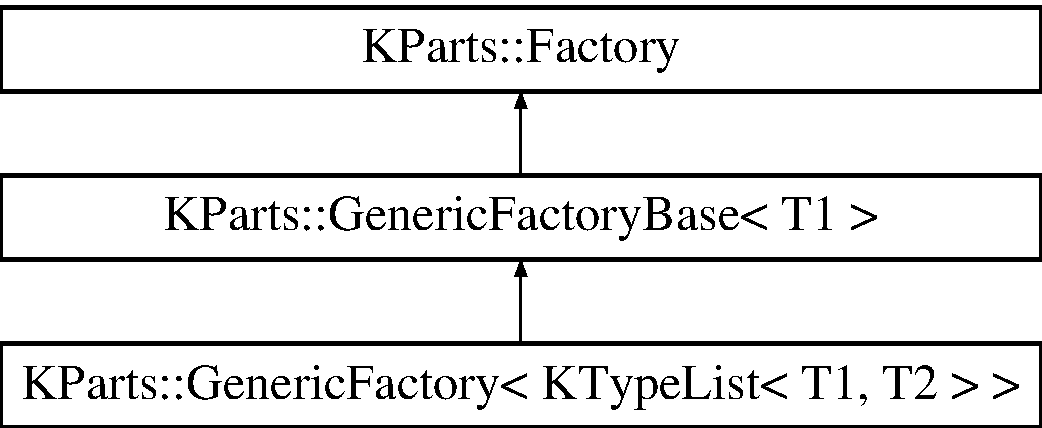
\includegraphics[height=4.000000cm]{classKParts_1_1GenericFactory_3_01KTypeList_3_01T1_00_01T2_01_4_01_4}
\end{center}
\end{figure}
\subsection*{Public Member Functions}
\begin{DoxyCompactItemize}
\item 
\hyperlink{classKParts_1_1GenericFactory_3_01KTypeList_3_01T1_00_01T2_01_4_01_4_addfaf3065f16712d09a7a63bee3fd116}{Generic\+Factory} ()
\item 
virtual \hyperlink{classKParts_1_1Part}{K\+Parts\+::\+Part} $\ast$ \hyperlink{classKParts_1_1GenericFactory_3_01KTypeList_3_01T1_00_01T2_01_4_01_4_aa3e8c27c10a09306951a2e63159a3d56}{create\+Part\+Object} (Q\+Widget $\ast$parent\+Widget, Q\+Object $\ast$parent, const char $\ast$class\+Name, const Q\+String\+List \&args)
\end{DoxyCompactItemize}
\subsection*{Additional Inherited Members}


\subsection{Detailed Description}
\subsubsection*{template$<$class T1, class T2$>$class K\+Parts\+::\+Generic\+Factory$<$ K\+Type\+List$<$ T1, T2 $>$ $>$}



Definition at line 136 of file genericfactory.\+h.



\subsection{Constructor \& Destructor Documentation}
\hypertarget{classKParts_1_1GenericFactory_3_01KTypeList_3_01T1_00_01T2_01_4_01_4_addfaf3065f16712d09a7a63bee3fd116}{\index{K\+Parts\+::\+Generic\+Factory$<$ K\+Type\+List$<$ T1, T2 $>$ $>$@{K\+Parts\+::\+Generic\+Factory$<$ K\+Type\+List$<$ T1, T2 $>$ $>$}!Generic\+Factory@{Generic\+Factory}}
\index{Generic\+Factory@{Generic\+Factory}!K\+Parts\+::\+Generic\+Factory$<$ K\+Type\+List$<$ T1, T2 $>$ $>$@{K\+Parts\+::\+Generic\+Factory$<$ K\+Type\+List$<$ T1, T2 $>$ $>$}}
\subsubsection[{Generic\+Factory}]{\setlength{\rightskip}{0pt plus 5cm}template$<$class T1 , class T2 $>$ {\bf K\+Parts\+::\+Generic\+Factory}$<$ K\+Type\+List$<$ T1, T2 $>$ $>$\+::{\bf Generic\+Factory} (
\begin{DoxyParamCaption}
{}
\end{DoxyParamCaption}
)\hspace{0.3cm}{\ttfamily [inline]}}}\label{classKParts_1_1GenericFactory_3_01KTypeList_3_01T1_00_01T2_01_4_01_4_addfaf3065f16712d09a7a63bee3fd116}


Definition at line 139 of file genericfactory.\+h.


\begin{DoxyCode}
139 \{ \}
\end{DoxyCode}


\subsection{Member Function Documentation}
\hypertarget{classKParts_1_1GenericFactory_3_01KTypeList_3_01T1_00_01T2_01_4_01_4_aa3e8c27c10a09306951a2e63159a3d56}{\index{K\+Parts\+::\+Generic\+Factory$<$ K\+Type\+List$<$ T1, T2 $>$ $>$@{K\+Parts\+::\+Generic\+Factory$<$ K\+Type\+List$<$ T1, T2 $>$ $>$}!create\+Part\+Object@{create\+Part\+Object}}
\index{create\+Part\+Object@{create\+Part\+Object}!K\+Parts\+::\+Generic\+Factory$<$ K\+Type\+List$<$ T1, T2 $>$ $>$@{K\+Parts\+::\+Generic\+Factory$<$ K\+Type\+List$<$ T1, T2 $>$ $>$}}
\subsubsection[{create\+Part\+Object}]{\setlength{\rightskip}{0pt plus 5cm}template$<$class T1 , class T2 $>$ virtual {\bf K\+Parts\+::\+Part}$\ast$ {\bf K\+Parts\+::\+Generic\+Factory}$<$ K\+Type\+List$<$ T1, T2 $>$ $>$\+::create\+Part\+Object (
\begin{DoxyParamCaption}
\item[{Q\+Widget $\ast$}]{parent\+Widget, }
\item[{Q\+Object $\ast$}]{parent, }
\item[{const char $\ast$}]{classname, }
\item[{const Q\+String\+List \&}]{args}
\end{DoxyParamCaption}
)\hspace{0.3cm}{\ttfamily [inline]}, {\ttfamily [virtual]}}}\label{classKParts_1_1GenericFactory_3_01KTypeList_3_01T1_00_01T2_01_4_01_4_aa3e8c27c10a09306951a2e63159a3d56}
Reimplement this method in your implementation to create the \hyperlink{classKParts_1_1Part}{Part}.

The Q\+String\+List can be used to pass additional arguments to the part. If the part needs additional arguments, it should take them as name=\char`\"{}value\char`\"{} pairs. This is the way additional arguments will get passed to the part from eg. khtml. You can for example emebed the part into H\+T\+M\+L by using the following code\+: 
\begin{DoxyCode}
<\textcolor{keywordtype}{object} type=\textcolor{stringliteral}{"my\_mimetype"} data=\textcolor{stringliteral}{"url\_to\_my\_data"}>
    <param name=\textcolor{stringliteral}{"name1"} value=\textcolor{stringliteral}{"value1"}>
    <param name=\textcolor{stringliteral}{"name2"} value=\textcolor{stringliteral}{"value2"}>
</\textcolor{keywordtype}{object}>
\end{DoxyCode}
 This could result in a call to 
\begin{DoxyCode}
\hyperlink{classKParts_1_1Factory_a41e7c93ddb621d17b7f380a9455ba2a8}{createPart}( parentWidget, parentObject, \textcolor{stringliteral}{"KParts::Part"},
            QStringList(\textcolor{stringliteral}{"name1="}value1\textcolor{stringliteral}{""}, \textcolor{stringliteral}{"name2="}value2\textcolor{stringliteral}{") );}
\end{DoxyCode}


\begin{DoxyReturn}{Returns}
the newly created part. 
\end{DoxyReturn}


Implements \hyperlink{classKParts_1_1Factory_a05e336b747b65776e31db466736570f2}{K\+Parts\+::\+Factory}.



Definition at line 141 of file genericfactory.\+h.


\begin{DoxyCode}
145         \{
146             QObject *\textcolor{keywordtype}{object} = KDEPrivate::MultiFactory< KTypeList<T1, T2> >::create( parentWidget,
147                                                                                      parent,
148                                                                                      className,
149                                                                                      args );
150 
151             \textcolor{comment}{// (this cast is guaranteed to work...)}
152             \hyperlink{classKParts_1_1Part}{KParts::Part} *part = \textcolor{keyword}{dynamic\_cast<}\hyperlink{classKParts_1_1Part}{KParts::Part} *\textcolor{keyword}{>}( object );
153 
154             \textcolor{keywordflow}{if} ( part && !qstrcmp( className, \textcolor{stringliteral}{"KParts::ReadOnlyPart"} ) )
155             \{
156                 \hyperlink{classKParts_1_1ReadWritePart}{KParts::ReadWritePart} *rwp = \textcolor{keyword}{dynamic\_cast<}
      \hyperlink{classKParts_1_1ReadWritePart}{KParts::ReadWritePart} *\textcolor{keyword}{>}( part );
157                 \textcolor{keywordflow}{if} ( rwp )
158                     rwp->\hyperlink{classKParts_1_1ReadWritePart_a5b8c2d4b35739c882dc67f0acf8096c2}{setReadWrite}( \textcolor{keyword}{false} );
159             \}
160             \textcolor{keywordflow}{return} part;
161         \}
\end{DoxyCode}


The documentation for this class was generated from the following file\+:\begin{DoxyCompactItemize}
\item 
/usr/include/kparts/\hyperlink{genericfactory_8h}{genericfactory.\+h}\end{DoxyCompactItemize}

\hypertarget{classKParts_1_1GenericFactoryBase}{\section{\-K\-Parts\-:\-:\-Generic\-Factory\-Base$<$ \-T $>$ \-Class \-Template \-Reference}
\label{classKParts_1_1GenericFactoryBase}\index{\-K\-Parts\-::\-Generic\-Factory\-Base$<$ T $>$@{\-K\-Parts\-::\-Generic\-Factory\-Base$<$ T $>$}}
}


{\ttfamily \#include $<$genericfactory.\-h$>$}

\-Inheritance diagram for \-K\-Parts\-:\-:\-Generic\-Factory\-Base$<$ \-T $>$\-:\begin{figure}[H]
\begin{center}
\leavevmode
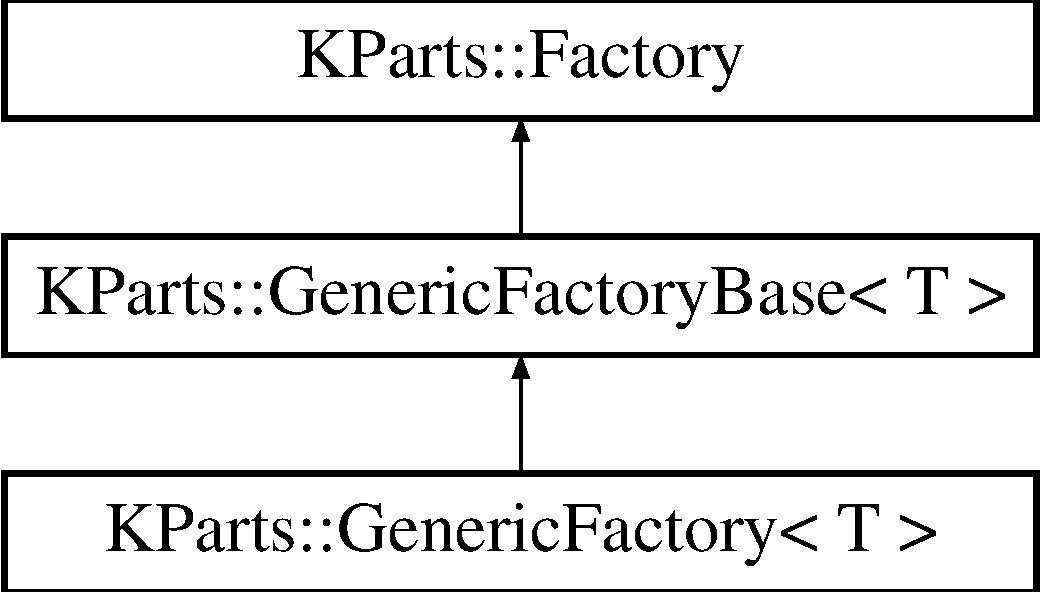
\includegraphics[height=3.000000cm]{classKParts_1_1GenericFactoryBase}
\end{center}
\end{figure}
\subsection*{\-Public \-Member \-Functions}
\begin{DoxyCompactItemize}
\item 
\hyperlink{classKParts_1_1GenericFactoryBase_af55233417c6cfae4f515ffe332987261}{\-Generic\-Factory\-Base} ()
\item 
virtual \hyperlink{classKParts_1_1GenericFactoryBase_a684bf9bd99f8c86d64a1fbdac6ee2901}{$\sim$\-Generic\-Factory\-Base} ()
\item 
virtual \-K\-Component\-Data \hyperlink{classKParts_1_1GenericFactoryBase_a0b1d32c7adf2255890bdd3898757feae}{part\-Component\-Data} ()
\end{DoxyCompactItemize}
\subsection*{\-Static \-Public \-Member \-Functions}
\begin{DoxyCompactItemize}
\item 
static const \-K\-Component\-Data \& \hyperlink{classKParts_1_1GenericFactoryBase_ad4a0ca70dec2fe8f4e0d4293e17eb776}{component\-Data} ()
\item 
static \-K\-About\-Data $\ast$ \hyperlink{classKParts_1_1GenericFactoryBase_ad5b89e87d73a76f3548c1afd09858020}{about\-Data} ()
\end{DoxyCompactItemize}
\subsection*{\-Protected \-Member \-Functions}
\begin{DoxyCompactItemize}
\item 
virtual \-K\-Component\-Data $\ast$ \hyperlink{classKParts_1_1GenericFactoryBase_ae90ec2009529241553290269f3108134}{create\-Component\-Data} ()
\end{DoxyCompactItemize}


\subsection{\-Detailed \-Description}
\subsubsection*{template$<$class \-T$>$class K\-Parts\-::\-Generic\-Factory\-Base$<$ T $>$}



\-Definition at line 35 of file genericfactory.\-h.



\subsection{\-Constructor \& \-Destructor \-Documentation}
\hypertarget{classKParts_1_1GenericFactoryBase_af55233417c6cfae4f515ffe332987261}{\index{\-K\-Parts\-::\-Generic\-Factory\-Base@{\-K\-Parts\-::\-Generic\-Factory\-Base}!\-Generic\-Factory\-Base@{\-Generic\-Factory\-Base}}
\index{\-Generic\-Factory\-Base@{\-Generic\-Factory\-Base}!KParts::GenericFactoryBase@{\-K\-Parts\-::\-Generic\-Factory\-Base}}
\subsubsection[{\-Generic\-Factory\-Base}]{\setlength{\rightskip}{0pt plus 5cm}template$<$class \-T$>$ {\bf \-K\-Parts\-::\-Generic\-Factory\-Base}$<$ \-T $>$\-::{\bf \-Generic\-Factory\-Base} (
\begin{DoxyParamCaption}
{}
\end{DoxyParamCaption}
)\hspace{0.3cm}{\ttfamily  \mbox{[}inline\mbox{]}}}}\label{classKParts_1_1GenericFactoryBase_af55233417c6cfae4f515ffe332987261}


\-Definition at line 38 of file genericfactory.\-h.


\begin{DoxyCode}
        {
            if ( s_self )
            {
                kWarning() << "KParts::GenericFactory instantiated more than
       once!";
            }
            s_self = this;
        }
\end{DoxyCode}
\hypertarget{classKParts_1_1GenericFactoryBase_a684bf9bd99f8c86d64a1fbdac6ee2901}{\index{\-K\-Parts\-::\-Generic\-Factory\-Base@{\-K\-Parts\-::\-Generic\-Factory\-Base}!$\sim$\-Generic\-Factory\-Base@{$\sim$\-Generic\-Factory\-Base}}
\index{$\sim$\-Generic\-Factory\-Base@{$\sim$\-Generic\-Factory\-Base}!KParts::GenericFactoryBase@{\-K\-Parts\-::\-Generic\-Factory\-Base}}
\subsubsection[{$\sim$\-Generic\-Factory\-Base}]{\setlength{\rightskip}{0pt plus 5cm}template$<$class \-T$>$ virtual {\bf \-K\-Parts\-::\-Generic\-Factory\-Base}$<$ \-T $>$\-::$\sim${\bf \-Generic\-Factory\-Base} (
\begin{DoxyParamCaption}
{}
\end{DoxyParamCaption}
)\hspace{0.3cm}{\ttfamily  \mbox{[}inline, virtual\mbox{]}}}}\label{classKParts_1_1GenericFactoryBase_a684bf9bd99f8c86d64a1fbdac6ee2901}


\-Definition at line 46 of file genericfactory.\-h.


\begin{DoxyCode}
        {
            delete s_aboutData;
            delete s_componentData;
            s_aboutData = 0;
            s_componentData = 0;
            s_self = 0;
        }
\end{DoxyCode}


\subsection{\-Member \-Function \-Documentation}
\hypertarget{classKParts_1_1GenericFactoryBase_ad5b89e87d73a76f3548c1afd09858020}{\index{\-K\-Parts\-::\-Generic\-Factory\-Base@{\-K\-Parts\-::\-Generic\-Factory\-Base}!about\-Data@{about\-Data}}
\index{about\-Data@{about\-Data}!KParts::GenericFactoryBase@{\-K\-Parts\-::\-Generic\-Factory\-Base}}
\subsubsection[{about\-Data}]{\setlength{\rightskip}{0pt plus 5cm}template$<$class T $>$ \-K\-About\-Data $\ast$ {\bf \-K\-Parts\-::\-Generic\-Factory\-Base}$<$ \-T $>$\-::{\bf about\-Data} (
\begin{DoxyParamCaption}
{}
\end{DoxyParamCaption}
)\hspace{0.3cm}{\ttfamily  \mbox{[}static\mbox{]}}}}\label{classKParts_1_1GenericFactoryBase_ad5b89e87d73a76f3548c1afd09858020}


\-Definition at line 202 of file genericfactory.\-h.


\begin{DoxyCode}
    {
        if ( !s_aboutData )
            s_aboutData = T::createAboutData();
        return s_aboutData;
    }
\end{DoxyCode}
\hypertarget{classKParts_1_1GenericFactoryBase_ad4a0ca70dec2fe8f4e0d4293e17eb776}{\index{\-K\-Parts\-::\-Generic\-Factory\-Base@{\-K\-Parts\-::\-Generic\-Factory\-Base}!component\-Data@{component\-Data}}
\index{component\-Data@{component\-Data}!KParts::GenericFactoryBase@{\-K\-Parts\-::\-Generic\-Factory\-Base}}
\subsubsection[{component\-Data}]{\setlength{\rightskip}{0pt plus 5cm}template$<$class T $>$ const \-K\-Component\-Data \& {\bf \-K\-Parts\-::\-Generic\-Factory\-Base}$<$ \-T $>$\-::{\bf component\-Data} (
\begin{DoxyParamCaption}
{}
\end{DoxyParamCaption}
)\hspace{0.3cm}{\ttfamily  \mbox{[}static\mbox{]}}}}\label{classKParts_1_1GenericFactoryBase_ad4a0ca70dec2fe8f4e0d4293e17eb776}


\-Definition at line 186 of file genericfactory.\-h.


\begin{DoxyCode}
    {
        if ( !s_componentData )
        {
            if ( s_self )
                s_componentData = s_self->createComponentData();
            else
                s_componentData = new KComponentData(aboutData());
        }
        return *s_componentData;
    }
\end{DoxyCode}
\hypertarget{classKParts_1_1GenericFactoryBase_ae90ec2009529241553290269f3108134}{\index{\-K\-Parts\-::\-Generic\-Factory\-Base@{\-K\-Parts\-::\-Generic\-Factory\-Base}!create\-Component\-Data@{create\-Component\-Data}}
\index{create\-Component\-Data@{create\-Component\-Data}!KParts::GenericFactoryBase@{\-K\-Parts\-::\-Generic\-Factory\-Base}}
\subsubsection[{create\-Component\-Data}]{\setlength{\rightskip}{0pt plus 5cm}template$<$class \-T$>$ virtual \-K\-Component\-Data$\ast$ {\bf \-K\-Parts\-::\-Generic\-Factory\-Base}$<$ \-T $>$\-::{\bf create\-Component\-Data} (
\begin{DoxyParamCaption}
{}
\end{DoxyParamCaption}
)\hspace{0.3cm}{\ttfamily  \mbox{[}inline, protected, virtual\mbox{]}}}}\label{classKParts_1_1GenericFactoryBase_ae90ec2009529241553290269f3108134}


\-Definition at line 64 of file genericfactory.\-h.


\begin{DoxyCode}
        {
            return new KComponentData(aboutData());
        }
\end{DoxyCode}
\hypertarget{classKParts_1_1GenericFactoryBase_a0b1d32c7adf2255890bdd3898757feae}{\index{\-K\-Parts\-::\-Generic\-Factory\-Base@{\-K\-Parts\-::\-Generic\-Factory\-Base}!part\-Component\-Data@{part\-Component\-Data}}
\index{part\-Component\-Data@{part\-Component\-Data}!KParts::GenericFactoryBase@{\-K\-Parts\-::\-Generic\-Factory\-Base}}
\subsubsection[{part\-Component\-Data}]{\setlength{\rightskip}{0pt plus 5cm}template$<$class \-T$>$ virtual \-K\-Component\-Data {\bf \-K\-Parts\-::\-Generic\-Factory\-Base}$<$ \-T $>$\-::{\bf part\-Component\-Data} (
\begin{DoxyParamCaption}
{}
\end{DoxyParamCaption}
)\hspace{0.3cm}{\ttfamily  \mbox{[}inline, virtual\mbox{]}}}}\label{classKParts_1_1GenericFactoryBase_a0b1d32c7adf2255890bdd3898757feae}
\-If you have a part contained in a shared library you might want to query for meta-\/information like the about-\/data, or the \-K\-Component\-Data in general. \-If the part is exported using \hyperlink{classKParts_1_1GenericFactory}{\-K\-Parts\-::\-Generic\-Factory} then this method will return the instance that belongs to the part without the need to instantiate the part component. 

\-Reimplemented from \hyperlink{classKParts_1_1Factory_a94c5c244737f0aa7788a1c114bc2acb9}{\-K\-Parts\-::\-Factory}.



\-Definition at line 57 of file genericfactory.\-h.


\begin{DoxyCode}
        {
            return componentData();
        }
\end{DoxyCode}


\-The documentation for this class was generated from the following file\-:\begin{DoxyCompactItemize}
\item 
/usr/include/kparts/\hyperlink{genericfactory_8h}{genericfactory.\-h}\end{DoxyCompactItemize}

\hypertarget{classKParts_1_1GUIActivateEvent}{\section{K\+Parts\+:\+:G\+U\+I\+Activate\+Event Class Reference}
\label{classKParts_1_1GUIActivateEvent}\index{K\+Parts\+::\+G\+U\+I\+Activate\+Event@{K\+Parts\+::\+G\+U\+I\+Activate\+Event}}
}


{\ttfamily \#include $<$event.\+h$>$}

Inheritance diagram for K\+Parts\+:\+:G\+U\+I\+Activate\+Event\+:\begin{figure}[H]
\begin{center}
\leavevmode
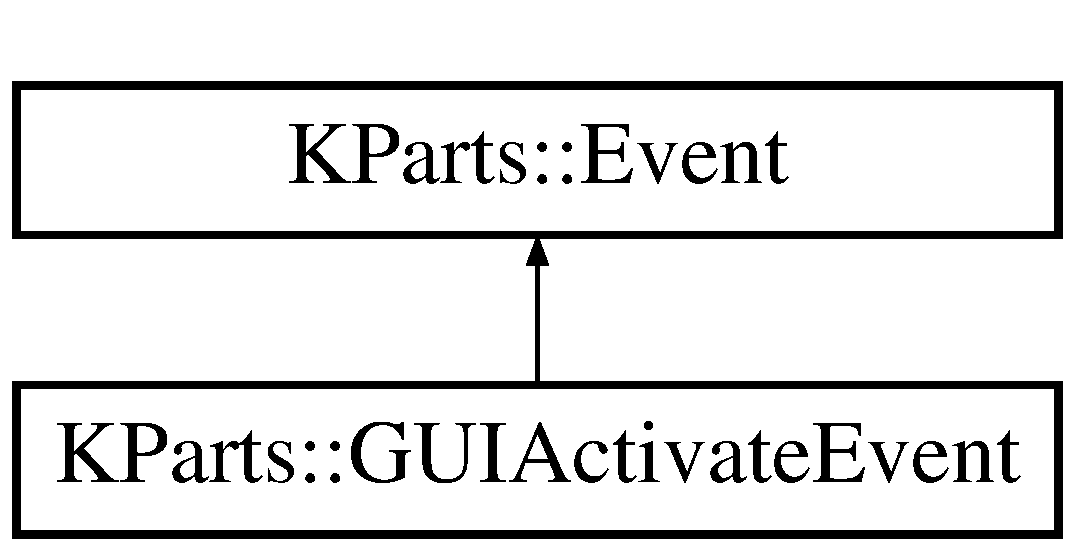
\includegraphics[height=3.000000cm]{classKParts_1_1GUIActivateEvent}
\end{center}
\end{figure}
\subsection*{Public Member Functions}
\begin{DoxyCompactItemize}
\item 
\hyperlink{classKParts_1_1GUIActivateEvent_a303f43218976a3af5612b127b7cdb06d}{G\+U\+I\+Activate\+Event} (bool \hyperlink{classKParts_1_1GUIActivateEvent_a6656d719771003b7877dc1137da82beb}{activated})
\item 
virtual \hyperlink{classKParts_1_1GUIActivateEvent_a26879d8d165ab17efcb773f0dce94d18}{$\sim$\+G\+U\+I\+Activate\+Event} ()
\item 
bool \hyperlink{classKParts_1_1GUIActivateEvent_a6656d719771003b7877dc1137da82beb}{activated} () const 
\end{DoxyCompactItemize}
\subsection*{Static Public Member Functions}
\begin{DoxyCompactItemize}
\item 
static bool \hyperlink{classKParts_1_1GUIActivateEvent_a360a35ee2b385c6b615e909e4a885e83}{test} (const Q\+Event $\ast$event)
\end{DoxyCompactItemize}


\subsection{Detailed Description}
This event is sent to a \hyperlink{classKParts_1_1Part}{Part} when its G\+U\+I has been activated or deactivated. This is related to \hyperlink{classKParts_1_1PartActivateEvent}{Part\+Activate\+Event}, but the difference is that \hyperlink{classKParts_1_1GUIActivateEvent}{G\+U\+I\+Activate\+Event} happens later (when the G\+U\+I is actually built), only for parts that have G\+U\+I elements, and only if using \hyperlink{classKParts_1_1MainWindow}{K\+Parts\+::\+Main\+Window}. \begin{DoxySeeAlso}{See Also}
\hyperlink{classKParts_1_1Part_a34b92f00459085ca7e05b7e8ee321347}{K\+Parts\+::\+Part\+::gui\+Activate\+Event()} 
\end{DoxySeeAlso}


Definition at line 59 of file event.\+h.



\subsection{Constructor \& Destructor Documentation}
\hypertarget{classKParts_1_1GUIActivateEvent_a303f43218976a3af5612b127b7cdb06d}{\index{K\+Parts\+::\+G\+U\+I\+Activate\+Event@{K\+Parts\+::\+G\+U\+I\+Activate\+Event}!G\+U\+I\+Activate\+Event@{G\+U\+I\+Activate\+Event}}
\index{G\+U\+I\+Activate\+Event@{G\+U\+I\+Activate\+Event}!K\+Parts\+::\+G\+U\+I\+Activate\+Event@{K\+Parts\+::\+G\+U\+I\+Activate\+Event}}
\subsubsection[{G\+U\+I\+Activate\+Event}]{\setlength{\rightskip}{0pt plus 5cm}K\+Parts\+::\+G\+U\+I\+Activate\+Event\+::\+G\+U\+I\+Activate\+Event (
\begin{DoxyParamCaption}
\item[{bool}]{activated}
\end{DoxyParamCaption}
)}}\label{classKParts_1_1GUIActivateEvent_a303f43218976a3af5612b127b7cdb06d}
\hypertarget{classKParts_1_1GUIActivateEvent_a26879d8d165ab17efcb773f0dce94d18}{\index{K\+Parts\+::\+G\+U\+I\+Activate\+Event@{K\+Parts\+::\+G\+U\+I\+Activate\+Event}!````~G\+U\+I\+Activate\+Event@{$\sim$\+G\+U\+I\+Activate\+Event}}
\index{````~G\+U\+I\+Activate\+Event@{$\sim$\+G\+U\+I\+Activate\+Event}!K\+Parts\+::\+G\+U\+I\+Activate\+Event@{K\+Parts\+::\+G\+U\+I\+Activate\+Event}}
\subsubsection[{$\sim$\+G\+U\+I\+Activate\+Event}]{\setlength{\rightskip}{0pt plus 5cm}virtual K\+Parts\+::\+G\+U\+I\+Activate\+Event\+::$\sim$\+G\+U\+I\+Activate\+Event (
\begin{DoxyParamCaption}
{}
\end{DoxyParamCaption}
)\hspace{0.3cm}{\ttfamily [virtual]}}}\label{classKParts_1_1GUIActivateEvent_a26879d8d165ab17efcb773f0dce94d18}


\subsection{Member Function Documentation}
\hypertarget{classKParts_1_1GUIActivateEvent_a6656d719771003b7877dc1137da82beb}{\index{K\+Parts\+::\+G\+U\+I\+Activate\+Event@{K\+Parts\+::\+G\+U\+I\+Activate\+Event}!activated@{activated}}
\index{activated@{activated}!K\+Parts\+::\+G\+U\+I\+Activate\+Event@{K\+Parts\+::\+G\+U\+I\+Activate\+Event}}
\subsubsection[{activated}]{\setlength{\rightskip}{0pt plus 5cm}bool K\+Parts\+::\+G\+U\+I\+Activate\+Event\+::activated (
\begin{DoxyParamCaption}
{}
\end{DoxyParamCaption}
) const}}\label{classKParts_1_1GUIActivateEvent_a6656d719771003b7877dc1137da82beb}
\hypertarget{classKParts_1_1GUIActivateEvent_a360a35ee2b385c6b615e909e4a885e83}{\index{K\+Parts\+::\+G\+U\+I\+Activate\+Event@{K\+Parts\+::\+G\+U\+I\+Activate\+Event}!test@{test}}
\index{test@{test}!K\+Parts\+::\+G\+U\+I\+Activate\+Event@{K\+Parts\+::\+G\+U\+I\+Activate\+Event}}
\subsubsection[{test}]{\setlength{\rightskip}{0pt plus 5cm}static bool K\+Parts\+::\+G\+U\+I\+Activate\+Event\+::test (
\begin{DoxyParamCaption}
\item[{const Q\+Event $\ast$}]{event}
\end{DoxyParamCaption}
)\hspace{0.3cm}{\ttfamily [static]}}}\label{classKParts_1_1GUIActivateEvent_a360a35ee2b385c6b615e909e4a885e83}


The documentation for this class was generated from the following file\+:\begin{DoxyCompactItemize}
\item 
/usr/include/kparts/\hyperlink{event_8h}{event.\+h}\end{DoxyCompactItemize}

\hypertarget{classKParts_1_1HistoryProvider}{\section{\-K\-Parts\-:\-:\-History\-Provider \-Class \-Reference}
\label{classKParts_1_1HistoryProvider}\index{\-K\-Parts\-::\-History\-Provider@{\-K\-Parts\-::\-History\-Provider}}
}


{\ttfamily \#include $<$historyprovider.\-h$>$}

\subsection*{\-Signals}
\begin{DoxyCompactItemize}
\item 
void \hyperlink{classKParts_1_1HistoryProvider_ac1328e387f0adb62419ddfdd74b1839e}{cleared} ()
\item 
void \hyperlink{classKParts_1_1HistoryProvider_adf153d0a7a3efcdaba20a86e323e115f}{updated} (const \-Q\-String\-List \&items)
\item 
void \hyperlink{classKParts_1_1HistoryProvider_a24304e5276a1f113314eb7b4e464828f}{inserted} (const \-Q\-String \&item)
\end{DoxyCompactItemize}
\subsection*{\-Public \-Member \-Functions}
\begin{DoxyCompactItemize}
\item 
virtual bool \hyperlink{classKParts_1_1HistoryProvider_a71a0c077cb80205334b56b0fd257a21d}{contains} (const \-Q\-String \&item) const 
\item 
virtual void \hyperlink{classKParts_1_1HistoryProvider_aace7bb17dca383aeecda7a34b9e0f40d}{insert} (const \-Q\-String \&item)
\item 
virtual void \hyperlink{classKParts_1_1HistoryProvider_a5852478b139f20346c53a30543748ed5}{remove} (const \-Q\-String \&item)
\item 
virtual void \hyperlink{classKParts_1_1HistoryProvider_ac377d52046a807032c21e17e8f03dd1e}{clear} ()
\end{DoxyCompactItemize}
\subsection*{\-Static \-Public \-Member \-Functions}
\begin{DoxyCompactItemize}
\item 
static \hyperlink{classKParts_1_1HistoryProvider}{\-History\-Provider} $\ast$ \hyperlink{classKParts_1_1HistoryProvider_a3c2fe96b915ebe5e310bbcbd8499002d}{self} ()
\item 
static bool \hyperlink{classKParts_1_1HistoryProvider_a5d7683f8804027d0a4106ace9a01c926}{exists} ()
\end{DoxyCompactItemize}
\subsection*{\-Protected \-Member \-Functions}
\begin{DoxyCompactItemize}
\item 
\hyperlink{classKParts_1_1HistoryProvider_a6b074dce67d7c90e6c795ef961272674}{\-History\-Provider} (\-Q\-Object $\ast$parent=0)
\item 
virtual \hyperlink{classKParts_1_1HistoryProvider_ad1c5d49be5dd48a6fd6776b55afa13d9}{$\sim$\-History\-Provider} ()
\end{DoxyCompactItemize}
\subsection*{\-Friends}
\begin{DoxyCompactItemize}
\item 
class \hyperlink{classKParts_1_1HistoryProvider_aa6bf68e5e8d7a54d38811147d3243489}{\-::\-K\-Parts\-::\-History\-Provider\-Private}
\end{DoxyCompactItemize}


\subsection{\-Detailed \-Description}
\-Basic class to manage a history of \char`\"{}items\char`\"{}. \-This class is only meant for fast lookup, if an item is in the history or not.

\-May be subclassed to implement a persistent history for example. \-For usage with khtml, just create your provider and call the \hyperlink{classKParts_1_1HistoryProvider}{\-History\-Provider} constructor \-\_\-before\-\_\- you do any khtml stuff. \-That way, khtml, using the \hyperlink{classKParts_1_1HistoryProvider_a3c2fe96b915ebe5e310bbcbd8499002d}{self()}-\/method, will use your subclassed provider.

\begin{DoxyAuthor}{\-Author}
\-Carsten \-Pfeiffer $<$\href{mailto:pfeiffer@kde.org}{\tt pfeiffer@kde.\-org}$>$ 
\end{DoxyAuthor}


\-Definition at line 42 of file historyprovider.\-h.



\subsection{\-Constructor \& \-Destructor \-Documentation}
\hypertarget{classKParts_1_1HistoryProvider_a6b074dce67d7c90e6c795ef961272674}{\index{\-K\-Parts\-::\-History\-Provider@{\-K\-Parts\-::\-History\-Provider}!\-History\-Provider@{\-History\-Provider}}
\index{\-History\-Provider@{\-History\-Provider}!KParts::HistoryProvider@{\-K\-Parts\-::\-History\-Provider}}
\subsubsection[{\-History\-Provider}]{\setlength{\rightskip}{0pt plus 5cm}{\bf \-K\-Parts\-::\-History\-Provider\-::\-History\-Provider} (
\begin{DoxyParamCaption}
\item[{\-Q\-Object $\ast$}]{parent = {\ttfamily 0}}
\end{DoxyParamCaption}
)\hspace{0.3cm}{\ttfamily  \mbox{[}protected\mbox{]}}}}\label{classKParts_1_1HistoryProvider_a6b074dce67d7c90e6c795ef961272674}
\-Creates a \-K\-History\-Provider with an optional parent and name \hypertarget{classKParts_1_1HistoryProvider_ad1c5d49be5dd48a6fd6776b55afa13d9}{\index{\-K\-Parts\-::\-History\-Provider@{\-K\-Parts\-::\-History\-Provider}!$\sim$\-History\-Provider@{$\sim$\-History\-Provider}}
\index{$\sim$\-History\-Provider@{$\sim$\-History\-Provider}!KParts::HistoryProvider@{\-K\-Parts\-::\-History\-Provider}}
\subsubsection[{$\sim$\-History\-Provider}]{\setlength{\rightskip}{0pt plus 5cm}virtual {\bf \-K\-Parts\-::\-History\-Provider\-::$\sim$\-History\-Provider} (
\begin{DoxyParamCaption}
{}
\end{DoxyParamCaption}
)\hspace{0.3cm}{\ttfamily  \mbox{[}protected, virtual\mbox{]}}}}\label{classKParts_1_1HistoryProvider_ad1c5d49be5dd48a6fd6776b55afa13d9}
\-Destroys the provider. 

\subsection{\-Member \-Function \-Documentation}
\hypertarget{classKParts_1_1HistoryProvider_ac377d52046a807032c21e17e8f03dd1e}{\index{\-K\-Parts\-::\-History\-Provider@{\-K\-Parts\-::\-History\-Provider}!clear@{clear}}
\index{clear@{clear}!KParts::HistoryProvider@{\-K\-Parts\-::\-History\-Provider}}
\subsubsection[{clear}]{\setlength{\rightskip}{0pt plus 5cm}virtual void {\bf \-K\-Parts\-::\-History\-Provider\-::clear} (
\begin{DoxyParamCaption}
{}
\end{DoxyParamCaption}
)\hspace{0.3cm}{\ttfamily  \mbox{[}virtual\mbox{]}}}}\label{classKParts_1_1HistoryProvider_ac377d52046a807032c21e17e8f03dd1e}
\-Clears the history. \-The \hyperlink{classKParts_1_1HistoryProvider_ac1328e387f0adb62419ddfdd74b1839e}{cleared()} signal is emitted after clearing. \hypertarget{classKParts_1_1HistoryProvider_ac1328e387f0adb62419ddfdd74b1839e}{\index{\-K\-Parts\-::\-History\-Provider@{\-K\-Parts\-::\-History\-Provider}!cleared@{cleared}}
\index{cleared@{cleared}!KParts::HistoryProvider@{\-K\-Parts\-::\-History\-Provider}}
\subsubsection[{cleared}]{\setlength{\rightskip}{0pt plus 5cm}void {\bf \-K\-Parts\-::\-History\-Provider\-::cleared} (
\begin{DoxyParamCaption}
{}
\end{DoxyParamCaption}
)\hspace{0.3cm}{\ttfamily  \mbox{[}signal\mbox{]}}}}\label{classKParts_1_1HistoryProvider_ac1328e387f0adb62419ddfdd74b1839e}
\-Emitted after the history has been cleared. \hypertarget{classKParts_1_1HistoryProvider_a71a0c077cb80205334b56b0fd257a21d}{\index{\-K\-Parts\-::\-History\-Provider@{\-K\-Parts\-::\-History\-Provider}!contains@{contains}}
\index{contains@{contains}!KParts::HistoryProvider@{\-K\-Parts\-::\-History\-Provider}}
\subsubsection[{contains}]{\setlength{\rightskip}{0pt plus 5cm}virtual bool {\bf \-K\-Parts\-::\-History\-Provider\-::contains} (
\begin{DoxyParamCaption}
\item[{const \-Q\-String \&}]{item}
\end{DoxyParamCaption}
) const\hspace{0.3cm}{\ttfamily  \mbox{[}virtual\mbox{]}}}}\label{classKParts_1_1HistoryProvider_a71a0c077cb80205334b56b0fd257a21d}
\begin{DoxyReturn}{\-Returns}
true if {\ttfamily item} is present in the history. 
\end{DoxyReturn}
\hypertarget{classKParts_1_1HistoryProvider_a5d7683f8804027d0a4106ace9a01c926}{\index{\-K\-Parts\-::\-History\-Provider@{\-K\-Parts\-::\-History\-Provider}!exists@{exists}}
\index{exists@{exists}!KParts::HistoryProvider@{\-K\-Parts\-::\-History\-Provider}}
\subsubsection[{exists}]{\setlength{\rightskip}{0pt plus 5cm}static bool {\bf \-K\-Parts\-::\-History\-Provider\-::exists} (
\begin{DoxyParamCaption}
{}
\end{DoxyParamCaption}
)\hspace{0.3cm}{\ttfamily  \mbox{[}static\mbox{]}}}}\label{classKParts_1_1HistoryProvider_a5d7683f8804027d0a4106ace9a01c926}
\begin{DoxyReturn}{\-Returns}
true if a provider has already been created. 
\end{DoxyReturn}
\begin{DoxySince}{\-Since}
4.\-4 
\end{DoxySince}
\hypertarget{classKParts_1_1HistoryProvider_aace7bb17dca383aeecda7a34b9e0f40d}{\index{\-K\-Parts\-::\-History\-Provider@{\-K\-Parts\-::\-History\-Provider}!insert@{insert}}
\index{insert@{insert}!KParts::HistoryProvider@{\-K\-Parts\-::\-History\-Provider}}
\subsubsection[{insert}]{\setlength{\rightskip}{0pt plus 5cm}virtual void {\bf \-K\-Parts\-::\-History\-Provider\-::insert} (
\begin{DoxyParamCaption}
\item[{const \-Q\-String \&}]{item}
\end{DoxyParamCaption}
)\hspace{0.3cm}{\ttfamily  \mbox{[}virtual\mbox{]}}}}\label{classKParts_1_1HistoryProvider_aace7bb17dca383aeecda7a34b9e0f40d}
\-Inserts {\ttfamily item} into the history. \hypertarget{classKParts_1_1HistoryProvider_a24304e5276a1f113314eb7b4e464828f}{\index{\-K\-Parts\-::\-History\-Provider@{\-K\-Parts\-::\-History\-Provider}!inserted@{inserted}}
\index{inserted@{inserted}!KParts::HistoryProvider@{\-K\-Parts\-::\-History\-Provider}}
\subsubsection[{inserted}]{\setlength{\rightskip}{0pt plus 5cm}void {\bf \-K\-Parts\-::\-History\-Provider\-::inserted} (
\begin{DoxyParamCaption}
\item[{const \-Q\-String \&}]{item}
\end{DoxyParamCaption}
)\hspace{0.3cm}{\ttfamily  \mbox{[}signal\mbox{]}}}}\label{classKParts_1_1HistoryProvider_a24304e5276a1f113314eb7b4e464828f}
\-Emitted after the item has been inserted \hypertarget{classKParts_1_1HistoryProvider_a5852478b139f20346c53a30543748ed5}{\index{\-K\-Parts\-::\-History\-Provider@{\-K\-Parts\-::\-History\-Provider}!remove@{remove}}
\index{remove@{remove}!KParts::HistoryProvider@{\-K\-Parts\-::\-History\-Provider}}
\subsubsection[{remove}]{\setlength{\rightskip}{0pt plus 5cm}virtual void {\bf \-K\-Parts\-::\-History\-Provider\-::remove} (
\begin{DoxyParamCaption}
\item[{const \-Q\-String \&}]{item}
\end{DoxyParamCaption}
)\hspace{0.3cm}{\ttfamily  \mbox{[}virtual\mbox{]}}}}\label{classKParts_1_1HistoryProvider_a5852478b139f20346c53a30543748ed5}
\-Removes {\ttfamily item} from the history. \hypertarget{classKParts_1_1HistoryProvider_a3c2fe96b915ebe5e310bbcbd8499002d}{\index{\-K\-Parts\-::\-History\-Provider@{\-K\-Parts\-::\-History\-Provider}!self@{self}}
\index{self@{self}!KParts::HistoryProvider@{\-K\-Parts\-::\-History\-Provider}}
\subsubsection[{self}]{\setlength{\rightskip}{0pt plus 5cm}static {\bf \-History\-Provider}$\ast$ {\bf \-K\-Parts\-::\-History\-Provider\-::self} (
\begin{DoxyParamCaption}
{}
\end{DoxyParamCaption}
)\hspace{0.3cm}{\ttfamily  \mbox{[}static\mbox{]}}}}\label{classKParts_1_1HistoryProvider_a3c2fe96b915ebe5e310bbcbd8499002d}
\hypertarget{classKParts_1_1HistoryProvider_adf153d0a7a3efcdaba20a86e323e115f}{\index{\-K\-Parts\-::\-History\-Provider@{\-K\-Parts\-::\-History\-Provider}!updated@{updated}}
\index{updated@{updated}!KParts::HistoryProvider@{\-K\-Parts\-::\-History\-Provider}}
\subsubsection[{updated}]{\setlength{\rightskip}{0pt plus 5cm}void {\bf \-K\-Parts\-::\-History\-Provider\-::updated} (
\begin{DoxyParamCaption}
\item[{const \-Q\-String\-List \&}]{items}
\end{DoxyParamCaption}
)\hspace{0.3cm}{\ttfamily  \mbox{[}signal\mbox{]}}}}\label{classKParts_1_1HistoryProvider_adf153d0a7a3efcdaba20a86e323e115f}
\-This signal is never emitted from this class, it is only meant as an interface for subclasses. \-Emit this signal to notify others that the history has changed. \-Put those items that were added or removed from the history into {\ttfamily items}. 

\subsection{\-Friends \-And \-Related \-Function \-Documentation}
\hypertarget{classKParts_1_1HistoryProvider_aa6bf68e5e8d7a54d38811147d3243489}{\index{\-K\-Parts\-::\-History\-Provider@{\-K\-Parts\-::\-History\-Provider}!\-::\-K\-Parts\-::\-History\-Provider\-Private@{\-::\-K\-Parts\-::\-History\-Provider\-Private}}
\index{\-::\-K\-Parts\-::\-History\-Provider\-Private@{\-::\-K\-Parts\-::\-History\-Provider\-Private}!KParts::HistoryProvider@{\-K\-Parts\-::\-History\-Provider}}
\subsubsection[{\-::\-K\-Parts\-::\-History\-Provider\-Private}]{\setlength{\rightskip}{0pt plus 5cm}friend class \-::\-K\-Parts\-::\-History\-Provider\-Private\hspace{0.3cm}{\ttfamily  \mbox{[}friend\mbox{]}}}}\label{classKParts_1_1HistoryProvider_aa6bf68e5e8d7a54d38811147d3243489}


\-Definition at line 45 of file historyprovider.\-h.



\-The documentation for this class was generated from the following file\-:\begin{DoxyCompactItemize}
\item 
/usr/include/kparts/\hyperlink{historyprovider_8h}{historyprovider.\-h}\end{DoxyCompactItemize}

\hypertarget{classKParts_1_1HtmlExtension}{\section{K\+Parts\+:\+:Html\+Extension Class Reference}
\label{classKParts_1_1HtmlExtension}\index{K\+Parts\+::\+Html\+Extension@{K\+Parts\+::\+Html\+Extension}}
}


an extension for \hyperlink{namespaceKParts}{K\+Parts} to provide H\+T\+M\+L-\/related features  




{\ttfamily \#include $<$htmlextension.\+h$>$}

Inheritance diagram for K\+Parts\+:\+:Html\+Extension\+:\begin{figure}[H]
\begin{center}
\leavevmode
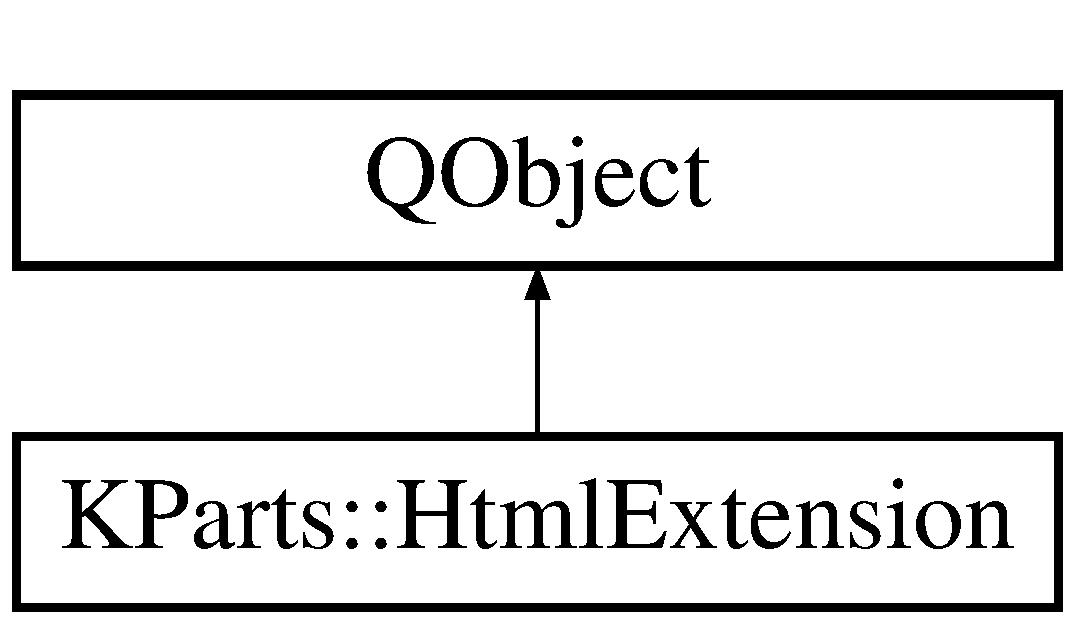
\includegraphics[height=2.000000cm]{classKParts_1_1HtmlExtension}
\end{center}
\end{figure}
\subsection*{Public Member Functions}
\begin{DoxyCompactItemize}
\item 
\hyperlink{classKParts_1_1HtmlExtension_ab75dcddad99744aad01a10b9b46b4f61}{Html\+Extension} (\hyperlink{classKParts_1_1ReadOnlyPart}{K\+Parts\+::\+Read\+Only\+Part} $\ast$parent)
\item 
\hyperlink{classKParts_1_1HtmlExtension_a090a296e890f968563d0352d4836efdd}{$\sim$\+Html\+Extension} ()
\item 
virtual K\+Url \hyperlink{classKParts_1_1HtmlExtension_a4be55820c257361f38ad9a595048bf5e}{base\+Url} () const =0
\item 
virtual bool \hyperlink{classKParts_1_1HtmlExtension_af3fe68c816bf92e14ceafdbf5179f134}{has\+Selection} () const 
\end{DoxyCompactItemize}
\subsection*{Static Public Member Functions}
\begin{DoxyCompactItemize}
\item 
static \hyperlink{classKParts_1_1HtmlExtension}{Html\+Extension} $\ast$ \hyperlink{classKParts_1_1HtmlExtension_a1008467fb117fa5dcf7cba422aa91f68}{child\+Object} (Q\+Object $\ast$obj)
\end{DoxyCompactItemize}


\subsection{Detailed Description}
an extension for \hyperlink{namespaceKParts}{K\+Parts} to provide H\+T\+M\+L-\/related features 

Use qobject\+\_\+cast to cast the extension to interesting interfaces, like qobject\+\_\+cast$<$\+K\+Parts\+::\+Selector\+Interface$>$.

\begin{DoxySince}{Since}
4.\+6 
\end{DoxySince}


Definition at line 45 of file htmlextension.\+h.



\subsection{Constructor \& Destructor Documentation}
\hypertarget{classKParts_1_1HtmlExtension_ab75dcddad99744aad01a10b9b46b4f61}{\index{K\+Parts\+::\+Html\+Extension@{K\+Parts\+::\+Html\+Extension}!Html\+Extension@{Html\+Extension}}
\index{Html\+Extension@{Html\+Extension}!K\+Parts\+::\+Html\+Extension@{K\+Parts\+::\+Html\+Extension}}
\subsubsection[{Html\+Extension}]{\setlength{\rightskip}{0pt plus 5cm}K\+Parts\+::\+Html\+Extension\+::\+Html\+Extension (
\begin{DoxyParamCaption}
\item[{{\bf K\+Parts\+::\+Read\+Only\+Part} $\ast$}]{parent}
\end{DoxyParamCaption}
)}}\label{classKParts_1_1HtmlExtension_ab75dcddad99744aad01a10b9b46b4f61}
\hypertarget{classKParts_1_1HtmlExtension_a090a296e890f968563d0352d4836efdd}{\index{K\+Parts\+::\+Html\+Extension@{K\+Parts\+::\+Html\+Extension}!````~Html\+Extension@{$\sim$\+Html\+Extension}}
\index{````~Html\+Extension@{$\sim$\+Html\+Extension}!K\+Parts\+::\+Html\+Extension@{K\+Parts\+::\+Html\+Extension}}
\subsubsection[{$\sim$\+Html\+Extension}]{\setlength{\rightskip}{0pt plus 5cm}K\+Parts\+::\+Html\+Extension\+::$\sim$\+Html\+Extension (
\begin{DoxyParamCaption}
{}
\end{DoxyParamCaption}
)}}\label{classKParts_1_1HtmlExtension_a090a296e890f968563d0352d4836efdd}


\subsection{Member Function Documentation}
\hypertarget{classKParts_1_1HtmlExtension_a4be55820c257361f38ad9a595048bf5e}{\index{K\+Parts\+::\+Html\+Extension@{K\+Parts\+::\+Html\+Extension}!base\+Url@{base\+Url}}
\index{base\+Url@{base\+Url}!K\+Parts\+::\+Html\+Extension@{K\+Parts\+::\+Html\+Extension}}
\subsubsection[{base\+Url}]{\setlength{\rightskip}{0pt plus 5cm}virtual K\+Url K\+Parts\+::\+Html\+Extension\+::base\+Url (
\begin{DoxyParamCaption}
{}
\end{DoxyParamCaption}
) const\hspace{0.3cm}{\ttfamily [pure virtual]}}}\label{classKParts_1_1HtmlExtension_a4be55820c257361f38ad9a595048bf5e}
Returns the current base url of the part that implements this extension.

This function is mostly used to resolve any relative U\+R\+Ls that might be returned when querying the part for links. \hypertarget{classKParts_1_1HtmlExtension_a1008467fb117fa5dcf7cba422aa91f68}{\index{K\+Parts\+::\+Html\+Extension@{K\+Parts\+::\+Html\+Extension}!child\+Object@{child\+Object}}
\index{child\+Object@{child\+Object}!K\+Parts\+::\+Html\+Extension@{K\+Parts\+::\+Html\+Extension}}
\subsubsection[{child\+Object}]{\setlength{\rightskip}{0pt plus 5cm}static {\bf Html\+Extension}$\ast$ K\+Parts\+::\+Html\+Extension\+::child\+Object (
\begin{DoxyParamCaption}
\item[{Q\+Object $\ast$}]{obj}
\end{DoxyParamCaption}
)\hspace{0.3cm}{\ttfamily [static]}}}\label{classKParts_1_1HtmlExtension_a1008467fb117fa5dcf7cba422aa91f68}
Queries {\ttfamily obj} for a child object which inherits from this \hyperlink{classKParts_1_1HtmlExtension}{Html\+Extension} class. \hypertarget{classKParts_1_1HtmlExtension_af3fe68c816bf92e14ceafdbf5179f134}{\index{K\+Parts\+::\+Html\+Extension@{K\+Parts\+::\+Html\+Extension}!has\+Selection@{has\+Selection}}
\index{has\+Selection@{has\+Selection}!K\+Parts\+::\+Html\+Extension@{K\+Parts\+::\+Html\+Extension}}
\subsubsection[{has\+Selection}]{\setlength{\rightskip}{0pt plus 5cm}virtual bool K\+Parts\+::\+Html\+Extension\+::has\+Selection (
\begin{DoxyParamCaption}
{}
\end{DoxyParamCaption}
) const\hspace{0.3cm}{\ttfamily [virtual]}}}\label{classKParts_1_1HtmlExtension_af3fe68c816bf92e14ceafdbf5179f134}
Returns true if portions of the content in the part that implements this extension are selected.

By default this function returns false. 

The documentation for this class was generated from the following file\+:\begin{DoxyCompactItemize}
\item 
/usr/include/kparts/\hyperlink{htmlextension_8h}{htmlextension.\+h}\end{DoxyCompactItemize}

\hypertarget{classKParts_1_1HtmlSettingsInterface}{\section{\-K\-Parts\-:\-:\-Html\-Settings\-Interface \-Class \-Reference}
\label{classKParts_1_1HtmlSettingsInterface}\index{\-K\-Parts\-::\-Html\-Settings\-Interface@{\-K\-Parts\-::\-Html\-Settings\-Interface}}
}


\-An interface for modifying the settings of browser engines.  




{\ttfamily \#include $<$htmlextension.\-h$>$}

\subsection*{\-Public \-Types}
\begin{DoxyCompactItemize}
\item 
enum \hyperlink{classKParts_1_1HtmlSettingsInterface_a62e44360376f423604c5c838ec0e312f}{\-Html\-Settings\-Type} \{ \*
\hyperlink{classKParts_1_1HtmlSettingsInterface_a62e44360376f423604c5c838ec0e312fa468efa7fce9486ff8b5d4a77a2a5c65a}{\-Auto\-Load\-Images}, 
\hyperlink{classKParts_1_1HtmlSettingsInterface_a62e44360376f423604c5c838ec0e312fa7ba037d57a86d39804300f97c2b179af}{\-Dns\-Prefetch\-Enabled}, 
\hyperlink{classKParts_1_1HtmlSettingsInterface_a62e44360376f423604c5c838ec0e312fa2ba86a71d6da5c17bbfc08e51ffe33fb}{\-Java\-Enabled}, 
\hyperlink{classKParts_1_1HtmlSettingsInterface_a62e44360376f423604c5c838ec0e312fa0f5a45bd022785fe4a0af542f3ba8225}{\-Javascript\-Enabled}, 
\*
\hyperlink{classKParts_1_1HtmlSettingsInterface_a62e44360376f423604c5c838ec0e312fa5686235c34f3d1d62a37ddd0cd1d54f1}{\-Meta\-Refresh\-Enabled}, 
\hyperlink{classKParts_1_1HtmlSettingsInterface_a62e44360376f423604c5c838ec0e312faed7f52d152accb3051b3771f29b704b2}{\-Plugins\-Enabled}, 
\hyperlink{classKParts_1_1HtmlSettingsInterface_a62e44360376f423604c5c838ec0e312fa1fcc78190cb150e98219649b5c04f0bb}{\-Private\-Browsing\-Enabled}, 
\hyperlink{classKParts_1_1HtmlSettingsInterface_a62e44360376f423604c5c838ec0e312fa7827dac10876b9a335cfeda7c4429787}{\-Offline\-Storage\-Database\-Enabled}, 
\*
\hyperlink{classKParts_1_1HtmlSettingsInterface_a62e44360376f423604c5c838ec0e312faca608c19402cb76cbe76f07f71878b00}{\-Offline\-Web\-Application\-Cache\-Enabled}, 
\hyperlink{classKParts_1_1HtmlSettingsInterface_a62e44360376f423604c5c838ec0e312fa8016ce157d4d18ea76fdf0e30ce168fb}{\-Local\-Storage\-Enabled}, 
\hyperlink{classKParts_1_1HtmlSettingsInterface_a62e44360376f423604c5c838ec0e312fa973267fbb4bfc8fbb2427efb759f1851}{\-User\-Defined\-Style\-Sheet\-U\-R\-L}
 \}
\item 
enum \hyperlink{classKParts_1_1HtmlSettingsInterface_af6b2303d6834ceff4d5251e10bd9d54b}{\-Java\-Script\-Advice} \{ \hyperlink{classKParts_1_1HtmlSettingsInterface_af6b2303d6834ceff4d5251e10bd9d54ba62d0bcc106417263cb46b6ced5bbfa49}{\-Java\-Script\-Dunno} = 0, 
\hyperlink{classKParts_1_1HtmlSettingsInterface_af6b2303d6834ceff4d5251e10bd9d54ba10e74b73b0ab617b5db0de123a3068ae}{\-Java\-Script\-Accept}, 
\hyperlink{classKParts_1_1HtmlSettingsInterface_af6b2303d6834ceff4d5251e10bd9d54ba8dd329b5196f7c0e2cf71338f2414479}{\-Java\-Script\-Reject}
 \}
\item 
enum \hyperlink{classKParts_1_1HtmlSettingsInterface_aab245c057a7179fc1bdc16e020750643}{\-J\-S\-Window\-Open\-Policy} \{ \hyperlink{classKParts_1_1HtmlSettingsInterface_aab245c057a7179fc1bdc16e020750643a079669fa32d8b86f6ae3b50241599431}{\-J\-S\-Window\-Open\-Allow} = 0, 
\hyperlink{classKParts_1_1HtmlSettingsInterface_aab245c057a7179fc1bdc16e020750643a3b5d146c17900bcb3ac5a3c40762400b}{\-J\-S\-Window\-Open\-Ask}, 
\hyperlink{classKParts_1_1HtmlSettingsInterface_aab245c057a7179fc1bdc16e020750643a7855bf2e8181c4ed74c47ef5c305ea66}{\-J\-S\-Window\-Open\-Deny}, 
\hyperlink{classKParts_1_1HtmlSettingsInterface_aab245c057a7179fc1bdc16e020750643aeb4533569b1d543c35bcbe2c13b4e0aa}{\-J\-S\-Window\-Open\-Smart}
 \}
\item 
enum \hyperlink{classKParts_1_1HtmlSettingsInterface_a88188ac567388141e0b1b988ae71961f}{\-J\-S\-Window\-Status\-Policy} \{ \hyperlink{classKParts_1_1HtmlSettingsInterface_a88188ac567388141e0b1b988ae71961fad04d2617a3d59e82bb71b11eb8f522c4}{\-J\-S\-Window\-Status\-Allow} = 0, 
\hyperlink{classKParts_1_1HtmlSettingsInterface_a88188ac567388141e0b1b988ae71961fa43c54134ec0c80999f2cf5ef0644ca71}{\-J\-S\-Window\-Status\-Ignore}
 \}
\item 
enum \hyperlink{classKParts_1_1HtmlSettingsInterface_a2774dbe8635ec916babf19de468d6c34}{\-J\-S\-Window\-Move\-Policy} \{ \hyperlink{classKParts_1_1HtmlSettingsInterface_a2774dbe8635ec916babf19de468d6c34a737536429edb7501bfc0a0e094c31005}{\-J\-S\-Window\-Move\-Allow} = 0, 
\hyperlink{classKParts_1_1HtmlSettingsInterface_a2774dbe8635ec916babf19de468d6c34affadad155cdf06f9eb98da8e1aa7cbb1}{\-J\-S\-Window\-Move\-Ignore}
 \}
\item 
enum \hyperlink{classKParts_1_1HtmlSettingsInterface_a0fcf7802e2f831ee1449e82713f6f359}{\-J\-S\-Window\-Resize\-Policy} \{ \hyperlink{classKParts_1_1HtmlSettingsInterface_a0fcf7802e2f831ee1449e82713f6f359ae2869f76bc4f064d4a60b89d09f043c8}{\-J\-S\-Window\-Resize\-Allow} = 0, 
\hyperlink{classKParts_1_1HtmlSettingsInterface_a0fcf7802e2f831ee1449e82713f6f359ae1c6f55c12b5abb6cafb06128334667a}{\-J\-S\-Window\-Resize\-Ignore}
 \}
\item 
enum \hyperlink{classKParts_1_1HtmlSettingsInterface_a3c00e5813af380f956480b47a76fdf8c}{\-J\-S\-Window\-Focus\-Policy} \{ \hyperlink{classKParts_1_1HtmlSettingsInterface_a3c00e5813af380f956480b47a76fdf8ca3eff6842f00de1e9ceef9a2f86e55e52}{\-J\-S\-Window\-Focus\-Allow} = 0, 
\hyperlink{classKParts_1_1HtmlSettingsInterface_a3c00e5813af380f956480b47a76fdf8cacc28bfbd61e4ae293d1201b4586b817a}{\-J\-S\-Window\-Focus\-Ignore}
 \}
\end{DoxyCompactItemize}
\subsection*{\-Public \-Member \-Functions}
\begin{DoxyCompactItemize}
\item 
virtual \hyperlink{classKParts_1_1HtmlSettingsInterface_a044f53f15e82bc3c209d578849812cfd}{$\sim$\-Html\-Settings\-Interface} ()
\item 
virtual \-Q\-Variant \hyperlink{classKParts_1_1HtmlSettingsInterface_a00b2a2f9ce6f7b505ab0bbfa4f71eca5}{html\-Settings\-Property} (\hyperlink{classKParts_1_1HtmlSettingsInterface_a62e44360376f423604c5c838ec0e312f}{\-Html\-Settings\-Type} type) const =0
\item 
virtual bool \hyperlink{classKParts_1_1HtmlSettingsInterface_ad345737d10028b838bb1324568d813f3}{set\-Html\-Settings\-Property} (\hyperlink{classKParts_1_1HtmlSettingsInterface_a62e44360376f423604c5c838ec0e312f}{\-Html\-Settings\-Type} type, const \-Q\-Variant \&value)=0
\end{DoxyCompactItemize}
\subsection*{\-Static \-Public \-Member \-Functions}
\begin{DoxyCompactItemize}
\item 
static \hyperlink{classKParts_1_1HtmlSettingsInterface_af6b2303d6834ceff4d5251e10bd9d54b}{\-Java\-Script\-Advice} \hyperlink{classKParts_1_1HtmlSettingsInterface_a6c0aaecc231a6005d37e7c4702f6d302}{text\-To\-Javascript\-Advice} (const \-Q\-String \&text)
\item 
static const char $\ast$ \hyperlink{classKParts_1_1HtmlSettingsInterface_a4f165269160ae72578b0c3c5a1fca22b}{javascript\-Advice\-To\-Text} (\hyperlink{classKParts_1_1HtmlSettingsInterface_af6b2303d6834ceff4d5251e10bd9d54b}{\-Java\-Script\-Advice} advice)
\item 
static void \hyperlink{classKParts_1_1HtmlSettingsInterface_a116a4f8ec62c3558ff75ae8099a2e030}{split\-Domain\-Advice} (const \-Q\-String \&text, \-Q\-String \&domain, \hyperlink{classKParts_1_1HtmlSettingsInterface_af6b2303d6834ceff4d5251e10bd9d54b}{\-Java\-Script\-Advice} \&java\-Advice, \hyperlink{classKParts_1_1HtmlSettingsInterface_af6b2303d6834ceff4d5251e10bd9d54b}{\-Java\-Script\-Advice} \&java\-Script\-Advice)
\end{DoxyCompactItemize}


\subsection{\-Detailed \-Description}
\-An interface for modifying the settings of browser engines. 

\-This interface provides a generic means for querying or changing the settings of browser engines that implement it.

\-To use this class simply cast an instance of the \-H\-T\-M\-L\-Extension object using qobject\-\_\-cast$<$\-K\-Parts\-::\-Html\-Settings\-Interface$>$.

\-Example\-: {\ttfamily  \-K\-Parts\-::\-H\-T\-M\-L\-Extension$\ast$ extension = \-K\-Parts\-::\-H\-T\-M\-L\-Extension\-::child\-Object(part); \hyperlink{classKParts_1_1HtmlSettingsInterface}{\-K\-Parts\-::\-Html\-Settings\-Interface}$\ast$ settings = qobject\-\_\-cast$<$\hyperlink{classKParts_1_1HtmlSettingsInterface}{\-K\-Parts\-::\-Html\-Settings\-Interface}$>$(extension); const bool auto\-Load\-Images = settings-\/$>$attribute(\-K\-Parts\-::\-Auto\-Load\-Images); }

\begin{DoxySince}{\-Since}
4.\-8.\-1 
\end{DoxySince}


\-Definition at line 245 of file htmlextension.\-h.



\subsection{\-Member \-Enumeration \-Documentation}
\hypertarget{classKParts_1_1HtmlSettingsInterface_a62e44360376f423604c5c838ec0e312f}{\index{\-K\-Parts\-::\-Html\-Settings\-Interface@{\-K\-Parts\-::\-Html\-Settings\-Interface}!\-Html\-Settings\-Type@{\-Html\-Settings\-Type}}
\index{\-Html\-Settings\-Type@{\-Html\-Settings\-Type}!KParts::HtmlSettingsInterface@{\-K\-Parts\-::\-Html\-Settings\-Interface}}
\subsubsection[{\-Html\-Settings\-Type}]{\setlength{\rightskip}{0pt plus 5cm}enum {\bf \-K\-Parts\-::\-Html\-Settings\-Interface\-::\-Html\-Settings\-Type}}}\label{classKParts_1_1HtmlSettingsInterface_a62e44360376f423604c5c838ec0e312f}
\-Settings attribute types. \begin{Desc}
\item[\-Enumerator\-: ]\par
\begin{description}
\index{\-Auto\-Load\-Images@{\-Auto\-Load\-Images}!\-K\-Parts\-::\-Html\-Settings\-Interface@{\-K\-Parts\-::\-Html\-Settings\-Interface}}\index{\-K\-Parts\-::\-Html\-Settings\-Interface@{\-K\-Parts\-::\-Html\-Settings\-Interface}!\-Auto\-Load\-Images@{\-Auto\-Load\-Images}}\item[{\em 
\hypertarget{classKParts_1_1HtmlSettingsInterface_a62e44360376f423604c5c838ec0e312fa468efa7fce9486ff8b5d4a77a2a5c65a}{\-Auto\-Load\-Images}\label{classKParts_1_1HtmlSettingsInterface_a62e44360376f423604c5c838ec0e312fa468efa7fce9486ff8b5d4a77a2a5c65a}
}]\index{\-Dns\-Prefetch\-Enabled@{\-Dns\-Prefetch\-Enabled}!\-K\-Parts\-::\-Html\-Settings\-Interface@{\-K\-Parts\-::\-Html\-Settings\-Interface}}\index{\-K\-Parts\-::\-Html\-Settings\-Interface@{\-K\-Parts\-::\-Html\-Settings\-Interface}!\-Dns\-Prefetch\-Enabled@{\-Dns\-Prefetch\-Enabled}}\item[{\em 
\hypertarget{classKParts_1_1HtmlSettingsInterface_a62e44360376f423604c5c838ec0e312fa7ba037d57a86d39804300f97c2b179af}{\-Dns\-Prefetch\-Enabled}\label{classKParts_1_1HtmlSettingsInterface_a62e44360376f423604c5c838ec0e312fa7ba037d57a86d39804300f97c2b179af}
}]\index{\-Java\-Enabled@{\-Java\-Enabled}!\-K\-Parts\-::\-Html\-Settings\-Interface@{\-K\-Parts\-::\-Html\-Settings\-Interface}}\index{\-K\-Parts\-::\-Html\-Settings\-Interface@{\-K\-Parts\-::\-Html\-Settings\-Interface}!\-Java\-Enabled@{\-Java\-Enabled}}\item[{\em 
\hypertarget{classKParts_1_1HtmlSettingsInterface_a62e44360376f423604c5c838ec0e312fa2ba86a71d6da5c17bbfc08e51ffe33fb}{\-Java\-Enabled}\label{classKParts_1_1HtmlSettingsInterface_a62e44360376f423604c5c838ec0e312fa2ba86a71d6da5c17bbfc08e51ffe33fb}
}]\index{\-Javascript\-Enabled@{\-Javascript\-Enabled}!\-K\-Parts\-::\-Html\-Settings\-Interface@{\-K\-Parts\-::\-Html\-Settings\-Interface}}\index{\-K\-Parts\-::\-Html\-Settings\-Interface@{\-K\-Parts\-::\-Html\-Settings\-Interface}!\-Javascript\-Enabled@{\-Javascript\-Enabled}}\item[{\em 
\hypertarget{classKParts_1_1HtmlSettingsInterface_a62e44360376f423604c5c838ec0e312fa0f5a45bd022785fe4a0af542f3ba8225}{\-Javascript\-Enabled}\label{classKParts_1_1HtmlSettingsInterface_a62e44360376f423604c5c838ec0e312fa0f5a45bd022785fe4a0af542f3ba8225}
}]\index{\-Meta\-Refresh\-Enabled@{\-Meta\-Refresh\-Enabled}!\-K\-Parts\-::\-Html\-Settings\-Interface@{\-K\-Parts\-::\-Html\-Settings\-Interface}}\index{\-K\-Parts\-::\-Html\-Settings\-Interface@{\-K\-Parts\-::\-Html\-Settings\-Interface}!\-Meta\-Refresh\-Enabled@{\-Meta\-Refresh\-Enabled}}\item[{\em 
\hypertarget{classKParts_1_1HtmlSettingsInterface_a62e44360376f423604c5c838ec0e312fa5686235c34f3d1d62a37ddd0cd1d54f1}{\-Meta\-Refresh\-Enabled}\label{classKParts_1_1HtmlSettingsInterface_a62e44360376f423604c5c838ec0e312fa5686235c34f3d1d62a37ddd0cd1d54f1}
}]\index{\-Plugins\-Enabled@{\-Plugins\-Enabled}!\-K\-Parts\-::\-Html\-Settings\-Interface@{\-K\-Parts\-::\-Html\-Settings\-Interface}}\index{\-K\-Parts\-::\-Html\-Settings\-Interface@{\-K\-Parts\-::\-Html\-Settings\-Interface}!\-Plugins\-Enabled@{\-Plugins\-Enabled}}\item[{\em 
\hypertarget{classKParts_1_1HtmlSettingsInterface_a62e44360376f423604c5c838ec0e312faed7f52d152accb3051b3771f29b704b2}{\-Plugins\-Enabled}\label{classKParts_1_1HtmlSettingsInterface_a62e44360376f423604c5c838ec0e312faed7f52d152accb3051b3771f29b704b2}
}]\index{\-Private\-Browsing\-Enabled@{\-Private\-Browsing\-Enabled}!\-K\-Parts\-::\-Html\-Settings\-Interface@{\-K\-Parts\-::\-Html\-Settings\-Interface}}\index{\-K\-Parts\-::\-Html\-Settings\-Interface@{\-K\-Parts\-::\-Html\-Settings\-Interface}!\-Private\-Browsing\-Enabled@{\-Private\-Browsing\-Enabled}}\item[{\em 
\hypertarget{classKParts_1_1HtmlSettingsInterface_a62e44360376f423604c5c838ec0e312fa1fcc78190cb150e98219649b5c04f0bb}{\-Private\-Browsing\-Enabled}\label{classKParts_1_1HtmlSettingsInterface_a62e44360376f423604c5c838ec0e312fa1fcc78190cb150e98219649b5c04f0bb}
}]\index{\-Offline\-Storage\-Database\-Enabled@{\-Offline\-Storage\-Database\-Enabled}!\-K\-Parts\-::\-Html\-Settings\-Interface@{\-K\-Parts\-::\-Html\-Settings\-Interface}}\index{\-K\-Parts\-::\-Html\-Settings\-Interface@{\-K\-Parts\-::\-Html\-Settings\-Interface}!\-Offline\-Storage\-Database\-Enabled@{\-Offline\-Storage\-Database\-Enabled}}\item[{\em 
\hypertarget{classKParts_1_1HtmlSettingsInterface_a62e44360376f423604c5c838ec0e312fa7827dac10876b9a335cfeda7c4429787}{\-Offline\-Storage\-Database\-Enabled}\label{classKParts_1_1HtmlSettingsInterface_a62e44360376f423604c5c838ec0e312fa7827dac10876b9a335cfeda7c4429787}
}]\index{\-Offline\-Web\-Application\-Cache\-Enabled@{\-Offline\-Web\-Application\-Cache\-Enabled}!\-K\-Parts\-::\-Html\-Settings\-Interface@{\-K\-Parts\-::\-Html\-Settings\-Interface}}\index{\-K\-Parts\-::\-Html\-Settings\-Interface@{\-K\-Parts\-::\-Html\-Settings\-Interface}!\-Offline\-Web\-Application\-Cache\-Enabled@{\-Offline\-Web\-Application\-Cache\-Enabled}}\item[{\em 
\hypertarget{classKParts_1_1HtmlSettingsInterface_a62e44360376f423604c5c838ec0e312faca608c19402cb76cbe76f07f71878b00}{\-Offline\-Web\-Application\-Cache\-Enabled}\label{classKParts_1_1HtmlSettingsInterface_a62e44360376f423604c5c838ec0e312faca608c19402cb76cbe76f07f71878b00}
}]\index{\-Local\-Storage\-Enabled@{\-Local\-Storage\-Enabled}!\-K\-Parts\-::\-Html\-Settings\-Interface@{\-K\-Parts\-::\-Html\-Settings\-Interface}}\index{\-K\-Parts\-::\-Html\-Settings\-Interface@{\-K\-Parts\-::\-Html\-Settings\-Interface}!\-Local\-Storage\-Enabled@{\-Local\-Storage\-Enabled}}\item[{\em 
\hypertarget{classKParts_1_1HtmlSettingsInterface_a62e44360376f423604c5c838ec0e312fa8016ce157d4d18ea76fdf0e30ce168fb}{\-Local\-Storage\-Enabled}\label{classKParts_1_1HtmlSettingsInterface_a62e44360376f423604c5c838ec0e312fa8016ce157d4d18ea76fdf0e30ce168fb}
}]\index{\-User\-Defined\-Style\-Sheet\-U\-R\-L@{\-User\-Defined\-Style\-Sheet\-U\-R\-L}!\-K\-Parts\-::\-Html\-Settings\-Interface@{\-K\-Parts\-::\-Html\-Settings\-Interface}}\index{\-K\-Parts\-::\-Html\-Settings\-Interface@{\-K\-Parts\-::\-Html\-Settings\-Interface}!\-User\-Defined\-Style\-Sheet\-U\-R\-L@{\-User\-Defined\-Style\-Sheet\-U\-R\-L}}\item[{\em 
\hypertarget{classKParts_1_1HtmlSettingsInterface_a62e44360376f423604c5c838ec0e312fa973267fbb4bfc8fbb2427efb759f1851}{\-User\-Defined\-Style\-Sheet\-U\-R\-L}\label{classKParts_1_1HtmlSettingsInterface_a62e44360376f423604c5c838ec0e312fa973267fbb4bfc8fbb2427efb759f1851}
}]\end{description}
\end{Desc}



\-Definition at line 251 of file htmlextension.\-h.


\begin{DoxyCode}
                          {
        AutoLoadImages,
        DnsPrefetchEnabled,
        JavaEnabled,
        JavascriptEnabled,
        MetaRefreshEnabled,
        PluginsEnabled,
        PrivateBrowsingEnabled,
        OfflineStorageDatabaseEnabled,
        OfflineWebApplicationCacheEnabled,
        LocalStorageEnabled,
        UserDefinedStyleSheetURL
    };
\end{DoxyCode}
\hypertarget{classKParts_1_1HtmlSettingsInterface_af6b2303d6834ceff4d5251e10bd9d54b}{\index{\-K\-Parts\-::\-Html\-Settings\-Interface@{\-K\-Parts\-::\-Html\-Settings\-Interface}!\-Java\-Script\-Advice@{\-Java\-Script\-Advice}}
\index{\-Java\-Script\-Advice@{\-Java\-Script\-Advice}!KParts::HtmlSettingsInterface@{\-K\-Parts\-::\-Html\-Settings\-Interface}}
\subsubsection[{\-Java\-Script\-Advice}]{\setlength{\rightskip}{0pt plus 5cm}enum {\bf \-K\-Parts\-::\-Html\-Settings\-Interface\-::\-Java\-Script\-Advice}}}\label{classKParts_1_1HtmlSettingsInterface_af6b2303d6834ceff4d5251e10bd9d54b}
\-This enum specifies whether \-Java/\-Java\-Script execution is allowed.

\begin{DoxySince}{\-Since}
4.\-8.\-2 
\end{DoxySince}
\begin{Desc}
\item[\-Enumerator\-: ]\par
\begin{description}
\index{\-Java\-Script\-Dunno@{\-Java\-Script\-Dunno}!\-K\-Parts\-::\-Html\-Settings\-Interface@{\-K\-Parts\-::\-Html\-Settings\-Interface}}\index{\-K\-Parts\-::\-Html\-Settings\-Interface@{\-K\-Parts\-::\-Html\-Settings\-Interface}!\-Java\-Script\-Dunno@{\-Java\-Script\-Dunno}}\item[{\em 
\hypertarget{classKParts_1_1HtmlSettingsInterface_af6b2303d6834ceff4d5251e10bd9d54ba62d0bcc106417263cb46b6ced5bbfa49}{\-Java\-Script\-Dunno}\label{classKParts_1_1HtmlSettingsInterface_af6b2303d6834ceff4d5251e10bd9d54ba62d0bcc106417263cb46b6ced5bbfa49}
}]\index{\-Java\-Script\-Accept@{\-Java\-Script\-Accept}!\-K\-Parts\-::\-Html\-Settings\-Interface@{\-K\-Parts\-::\-Html\-Settings\-Interface}}\index{\-K\-Parts\-::\-Html\-Settings\-Interface@{\-K\-Parts\-::\-Html\-Settings\-Interface}!\-Java\-Script\-Accept@{\-Java\-Script\-Accept}}\item[{\em 
\hypertarget{classKParts_1_1HtmlSettingsInterface_af6b2303d6834ceff4d5251e10bd9d54ba10e74b73b0ab617b5db0de123a3068ae}{\-Java\-Script\-Accept}\label{classKParts_1_1HtmlSettingsInterface_af6b2303d6834ceff4d5251e10bd9d54ba10e74b73b0ab617b5db0de123a3068ae}
}]\index{\-Java\-Script\-Reject@{\-Java\-Script\-Reject}!\-K\-Parts\-::\-Html\-Settings\-Interface@{\-K\-Parts\-::\-Html\-Settings\-Interface}}\index{\-K\-Parts\-::\-Html\-Settings\-Interface@{\-K\-Parts\-::\-Html\-Settings\-Interface}!\-Java\-Script\-Reject@{\-Java\-Script\-Reject}}\item[{\em 
\hypertarget{classKParts_1_1HtmlSettingsInterface_af6b2303d6834ceff4d5251e10bd9d54ba8dd329b5196f7c0e2cf71338f2414479}{\-Java\-Script\-Reject}\label{classKParts_1_1HtmlSettingsInterface_af6b2303d6834ceff4d5251e10bd9d54ba8dd329b5196f7c0e2cf71338f2414479}
}]\end{description}
\end{Desc}



\-Definition at line 270 of file htmlextension.\-h.


\begin{DoxyCode}
                          {
        JavaScriptDunno=0,
        JavaScriptAccept,
        JavaScriptReject
    };
\end{DoxyCode}
\hypertarget{classKParts_1_1HtmlSettingsInterface_a3c00e5813af380f956480b47a76fdf8c}{\index{\-K\-Parts\-::\-Html\-Settings\-Interface@{\-K\-Parts\-::\-Html\-Settings\-Interface}!\-J\-S\-Window\-Focus\-Policy@{\-J\-S\-Window\-Focus\-Policy}}
\index{\-J\-S\-Window\-Focus\-Policy@{\-J\-S\-Window\-Focus\-Policy}!KParts::HtmlSettingsInterface@{\-K\-Parts\-::\-Html\-Settings\-Interface}}
\subsubsection[{\-J\-S\-Window\-Focus\-Policy}]{\setlength{\rightskip}{0pt plus 5cm}enum {\bf \-K\-Parts\-::\-Html\-Settings\-Interface\-::\-J\-S\-Window\-Focus\-Policy}}}\label{classKParts_1_1HtmlSettingsInterface_a3c00e5813af380f956480b47a76fdf8c}
\-This enum specifies the policy for window.\-focus

\begin{DoxySince}{\-Since}
4.\-8.\-2 
\end{DoxySince}
\begin{Desc}
\item[\-Enumerator\-: ]\par
\begin{description}
\index{\-J\-S\-Window\-Focus\-Allow@{\-J\-S\-Window\-Focus\-Allow}!\-K\-Parts\-::\-Html\-Settings\-Interface@{\-K\-Parts\-::\-Html\-Settings\-Interface}}\index{\-K\-Parts\-::\-Html\-Settings\-Interface@{\-K\-Parts\-::\-Html\-Settings\-Interface}!\-J\-S\-Window\-Focus\-Allow@{\-J\-S\-Window\-Focus\-Allow}}\item[{\em 
\hypertarget{classKParts_1_1HtmlSettingsInterface_a3c00e5813af380f956480b47a76fdf8ca3eff6842f00de1e9ceef9a2f86e55e52}{\-J\-S\-Window\-Focus\-Allow}\label{classKParts_1_1HtmlSettingsInterface_a3c00e5813af380f956480b47a76fdf8ca3eff6842f00de1e9ceef9a2f86e55e52}
}]\index{\-J\-S\-Window\-Focus\-Ignore@{\-J\-S\-Window\-Focus\-Ignore}!\-K\-Parts\-::\-Html\-Settings\-Interface@{\-K\-Parts\-::\-Html\-Settings\-Interface}}\index{\-K\-Parts\-::\-Html\-Settings\-Interface@{\-K\-Parts\-::\-Html\-Settings\-Interface}!\-J\-S\-Window\-Focus\-Ignore@{\-J\-S\-Window\-Focus\-Ignore}}\item[{\em 
\hypertarget{classKParts_1_1HtmlSettingsInterface_a3c00e5813af380f956480b47a76fdf8cacc28bfbd61e4ae293d1201b4586b817a}{\-J\-S\-Window\-Focus\-Ignore}\label{classKParts_1_1HtmlSettingsInterface_a3c00e5813af380f956480b47a76fdf8cacc28bfbd61e4ae293d1201b4586b817a}
}]\end{description}
\end{Desc}



\-Definition at line 323 of file htmlextension.\-h.


\begin{DoxyCode}
                             {
        JSWindowFocusAllow=0,
        JSWindowFocusIgnore
    };
\end{DoxyCode}
\hypertarget{classKParts_1_1HtmlSettingsInterface_a2774dbe8635ec916babf19de468d6c34}{\index{\-K\-Parts\-::\-Html\-Settings\-Interface@{\-K\-Parts\-::\-Html\-Settings\-Interface}!\-J\-S\-Window\-Move\-Policy@{\-J\-S\-Window\-Move\-Policy}}
\index{\-J\-S\-Window\-Move\-Policy@{\-J\-S\-Window\-Move\-Policy}!KParts::HtmlSettingsInterface@{\-K\-Parts\-::\-Html\-Settings\-Interface}}
\subsubsection[{\-J\-S\-Window\-Move\-Policy}]{\setlength{\rightskip}{0pt plus 5cm}enum {\bf \-K\-Parts\-::\-Html\-Settings\-Interface\-::\-J\-S\-Window\-Move\-Policy}}}\label{classKParts_1_1HtmlSettingsInterface_a2774dbe8635ec916babf19de468d6c34}
\-This enum specifies the policy for window.\-move\-By and .move\-To

\begin{DoxySince}{\-Since}
4.\-8.\-2 
\end{DoxySince}
\begin{Desc}
\item[\-Enumerator\-: ]\par
\begin{description}
\index{\-J\-S\-Window\-Move\-Allow@{\-J\-S\-Window\-Move\-Allow}!\-K\-Parts\-::\-Html\-Settings\-Interface@{\-K\-Parts\-::\-Html\-Settings\-Interface}}\index{\-K\-Parts\-::\-Html\-Settings\-Interface@{\-K\-Parts\-::\-Html\-Settings\-Interface}!\-J\-S\-Window\-Move\-Allow@{\-J\-S\-Window\-Move\-Allow}}\item[{\em 
\hypertarget{classKParts_1_1HtmlSettingsInterface_a2774dbe8635ec916babf19de468d6c34a737536429edb7501bfc0a0e094c31005}{\-J\-S\-Window\-Move\-Allow}\label{classKParts_1_1HtmlSettingsInterface_a2774dbe8635ec916babf19de468d6c34a737536429edb7501bfc0a0e094c31005}
}]\index{\-J\-S\-Window\-Move\-Ignore@{\-J\-S\-Window\-Move\-Ignore}!\-K\-Parts\-::\-Html\-Settings\-Interface@{\-K\-Parts\-::\-Html\-Settings\-Interface}}\index{\-K\-Parts\-::\-Html\-Settings\-Interface@{\-K\-Parts\-::\-Html\-Settings\-Interface}!\-J\-S\-Window\-Move\-Ignore@{\-J\-S\-Window\-Move\-Ignore}}\item[{\em 
\hypertarget{classKParts_1_1HtmlSettingsInterface_a2774dbe8635ec916babf19de468d6c34affadad155cdf06f9eb98da8e1aa7cbb1}{\-J\-S\-Window\-Move\-Ignore}\label{classKParts_1_1HtmlSettingsInterface_a2774dbe8635ec916babf19de468d6c34affadad155cdf06f9eb98da8e1aa7cbb1}
}]\end{description}
\end{Desc}



\-Definition at line 303 of file htmlextension.\-h.


\begin{DoxyCode}
                            {
        JSWindowMoveAllow=0,
        JSWindowMoveIgnore
    };
\end{DoxyCode}
\hypertarget{classKParts_1_1HtmlSettingsInterface_aab245c057a7179fc1bdc16e020750643}{\index{\-K\-Parts\-::\-Html\-Settings\-Interface@{\-K\-Parts\-::\-Html\-Settings\-Interface}!\-J\-S\-Window\-Open\-Policy@{\-J\-S\-Window\-Open\-Policy}}
\index{\-J\-S\-Window\-Open\-Policy@{\-J\-S\-Window\-Open\-Policy}!KParts::HtmlSettingsInterface@{\-K\-Parts\-::\-Html\-Settings\-Interface}}
\subsubsection[{\-J\-S\-Window\-Open\-Policy}]{\setlength{\rightskip}{0pt plus 5cm}enum {\bf \-K\-Parts\-::\-Html\-Settings\-Interface\-::\-J\-S\-Window\-Open\-Policy}}}\label{classKParts_1_1HtmlSettingsInterface_aab245c057a7179fc1bdc16e020750643}
\-This enum specifies the policy for window.\-open

\begin{DoxySince}{\-Since}
4.\-8.\-2 
\end{DoxySince}
\begin{Desc}
\item[\-Enumerator\-: ]\par
\begin{description}
\index{\-J\-S\-Window\-Open\-Allow@{\-J\-S\-Window\-Open\-Allow}!\-K\-Parts\-::\-Html\-Settings\-Interface@{\-K\-Parts\-::\-Html\-Settings\-Interface}}\index{\-K\-Parts\-::\-Html\-Settings\-Interface@{\-K\-Parts\-::\-Html\-Settings\-Interface}!\-J\-S\-Window\-Open\-Allow@{\-J\-S\-Window\-Open\-Allow}}\item[{\em 
\hypertarget{classKParts_1_1HtmlSettingsInterface_aab245c057a7179fc1bdc16e020750643a079669fa32d8b86f6ae3b50241599431}{\-J\-S\-Window\-Open\-Allow}\label{classKParts_1_1HtmlSettingsInterface_aab245c057a7179fc1bdc16e020750643a079669fa32d8b86f6ae3b50241599431}
}]\index{\-J\-S\-Window\-Open\-Ask@{\-J\-S\-Window\-Open\-Ask}!\-K\-Parts\-::\-Html\-Settings\-Interface@{\-K\-Parts\-::\-Html\-Settings\-Interface}}\index{\-K\-Parts\-::\-Html\-Settings\-Interface@{\-K\-Parts\-::\-Html\-Settings\-Interface}!\-J\-S\-Window\-Open\-Ask@{\-J\-S\-Window\-Open\-Ask}}\item[{\em 
\hypertarget{classKParts_1_1HtmlSettingsInterface_aab245c057a7179fc1bdc16e020750643a3b5d146c17900bcb3ac5a3c40762400b}{\-J\-S\-Window\-Open\-Ask}\label{classKParts_1_1HtmlSettingsInterface_aab245c057a7179fc1bdc16e020750643a3b5d146c17900bcb3ac5a3c40762400b}
}]\index{\-J\-S\-Window\-Open\-Deny@{\-J\-S\-Window\-Open\-Deny}!\-K\-Parts\-::\-Html\-Settings\-Interface@{\-K\-Parts\-::\-Html\-Settings\-Interface}}\index{\-K\-Parts\-::\-Html\-Settings\-Interface@{\-K\-Parts\-::\-Html\-Settings\-Interface}!\-J\-S\-Window\-Open\-Deny@{\-J\-S\-Window\-Open\-Deny}}\item[{\em 
\hypertarget{classKParts_1_1HtmlSettingsInterface_aab245c057a7179fc1bdc16e020750643a7855bf2e8181c4ed74c47ef5c305ea66}{\-J\-S\-Window\-Open\-Deny}\label{classKParts_1_1HtmlSettingsInterface_aab245c057a7179fc1bdc16e020750643a7855bf2e8181c4ed74c47ef5c305ea66}
}]\index{\-J\-S\-Window\-Open\-Smart@{\-J\-S\-Window\-Open\-Smart}!\-K\-Parts\-::\-Html\-Settings\-Interface@{\-K\-Parts\-::\-Html\-Settings\-Interface}}\index{\-K\-Parts\-::\-Html\-Settings\-Interface@{\-K\-Parts\-::\-Html\-Settings\-Interface}!\-J\-S\-Window\-Open\-Smart@{\-J\-S\-Window\-Open\-Smart}}\item[{\em 
\hypertarget{classKParts_1_1HtmlSettingsInterface_aab245c057a7179fc1bdc16e020750643aeb4533569b1d543c35bcbe2c13b4e0aa}{\-J\-S\-Window\-Open\-Smart}\label{classKParts_1_1HtmlSettingsInterface_aab245c057a7179fc1bdc16e020750643aeb4533569b1d543c35bcbe2c13b4e0aa}
}]\end{description}
\end{Desc}



\-Definition at line 281 of file htmlextension.\-h.


\begin{DoxyCode}
                            {
        JSWindowOpenAllow=0,
        JSWindowOpenAsk,
        JSWindowOpenDeny,
        JSWindowOpenSmart
    };
\end{DoxyCode}
\hypertarget{classKParts_1_1HtmlSettingsInterface_a0fcf7802e2f831ee1449e82713f6f359}{\index{\-K\-Parts\-::\-Html\-Settings\-Interface@{\-K\-Parts\-::\-Html\-Settings\-Interface}!\-J\-S\-Window\-Resize\-Policy@{\-J\-S\-Window\-Resize\-Policy}}
\index{\-J\-S\-Window\-Resize\-Policy@{\-J\-S\-Window\-Resize\-Policy}!KParts::HtmlSettingsInterface@{\-K\-Parts\-::\-Html\-Settings\-Interface}}
\subsubsection[{\-J\-S\-Window\-Resize\-Policy}]{\setlength{\rightskip}{0pt plus 5cm}enum {\bf \-K\-Parts\-::\-Html\-Settings\-Interface\-::\-J\-S\-Window\-Resize\-Policy}}}\label{classKParts_1_1HtmlSettingsInterface_a0fcf7802e2f831ee1449e82713f6f359}
\-This enum specifies the policy for window.\-resize\-By and .resize\-To

\begin{DoxySince}{\-Since}
4.\-8.\-2 
\end{DoxySince}
\begin{Desc}
\item[\-Enumerator\-: ]\par
\begin{description}
\index{\-J\-S\-Window\-Resize\-Allow@{\-J\-S\-Window\-Resize\-Allow}!\-K\-Parts\-::\-Html\-Settings\-Interface@{\-K\-Parts\-::\-Html\-Settings\-Interface}}\index{\-K\-Parts\-::\-Html\-Settings\-Interface@{\-K\-Parts\-::\-Html\-Settings\-Interface}!\-J\-S\-Window\-Resize\-Allow@{\-J\-S\-Window\-Resize\-Allow}}\item[{\em 
\hypertarget{classKParts_1_1HtmlSettingsInterface_a0fcf7802e2f831ee1449e82713f6f359ae2869f76bc4f064d4a60b89d09f043c8}{\-J\-S\-Window\-Resize\-Allow}\label{classKParts_1_1HtmlSettingsInterface_a0fcf7802e2f831ee1449e82713f6f359ae2869f76bc4f064d4a60b89d09f043c8}
}]\index{\-J\-S\-Window\-Resize\-Ignore@{\-J\-S\-Window\-Resize\-Ignore}!\-K\-Parts\-::\-Html\-Settings\-Interface@{\-K\-Parts\-::\-Html\-Settings\-Interface}}\index{\-K\-Parts\-::\-Html\-Settings\-Interface@{\-K\-Parts\-::\-Html\-Settings\-Interface}!\-J\-S\-Window\-Resize\-Ignore@{\-J\-S\-Window\-Resize\-Ignore}}\item[{\em 
\hypertarget{classKParts_1_1HtmlSettingsInterface_a0fcf7802e2f831ee1449e82713f6f359ae1c6f55c12b5abb6cafb06128334667a}{\-J\-S\-Window\-Resize\-Ignore}\label{classKParts_1_1HtmlSettingsInterface_a0fcf7802e2f831ee1449e82713f6f359ae1c6f55c12b5abb6cafb06128334667a}
}]\end{description}
\end{Desc}



\-Definition at line 313 of file htmlextension.\-h.


\begin{DoxyCode}
                              {
        JSWindowResizeAllow=0,
        JSWindowResizeIgnore
    };
\end{DoxyCode}
\hypertarget{classKParts_1_1HtmlSettingsInterface_a88188ac567388141e0b1b988ae71961f}{\index{\-K\-Parts\-::\-Html\-Settings\-Interface@{\-K\-Parts\-::\-Html\-Settings\-Interface}!\-J\-S\-Window\-Status\-Policy@{\-J\-S\-Window\-Status\-Policy}}
\index{\-J\-S\-Window\-Status\-Policy@{\-J\-S\-Window\-Status\-Policy}!KParts::HtmlSettingsInterface@{\-K\-Parts\-::\-Html\-Settings\-Interface}}
\subsubsection[{\-J\-S\-Window\-Status\-Policy}]{\setlength{\rightskip}{0pt plus 5cm}enum {\bf \-K\-Parts\-::\-Html\-Settings\-Interface\-::\-J\-S\-Window\-Status\-Policy}}}\label{classKParts_1_1HtmlSettingsInterface_a88188ac567388141e0b1b988ae71961f}
\-This enum specifies the policy for window.\-status and .default\-Status

\begin{DoxySince}{\-Since}
4.\-8.\-2 
\end{DoxySince}
\begin{Desc}
\item[\-Enumerator\-: ]\par
\begin{description}
\index{\-J\-S\-Window\-Status\-Allow@{\-J\-S\-Window\-Status\-Allow}!\-K\-Parts\-::\-Html\-Settings\-Interface@{\-K\-Parts\-::\-Html\-Settings\-Interface}}\index{\-K\-Parts\-::\-Html\-Settings\-Interface@{\-K\-Parts\-::\-Html\-Settings\-Interface}!\-J\-S\-Window\-Status\-Allow@{\-J\-S\-Window\-Status\-Allow}}\item[{\em 
\hypertarget{classKParts_1_1HtmlSettingsInterface_a88188ac567388141e0b1b988ae71961fad04d2617a3d59e82bb71b11eb8f522c4}{\-J\-S\-Window\-Status\-Allow}\label{classKParts_1_1HtmlSettingsInterface_a88188ac567388141e0b1b988ae71961fad04d2617a3d59e82bb71b11eb8f522c4}
}]\index{\-J\-S\-Window\-Status\-Ignore@{\-J\-S\-Window\-Status\-Ignore}!\-K\-Parts\-::\-Html\-Settings\-Interface@{\-K\-Parts\-::\-Html\-Settings\-Interface}}\index{\-K\-Parts\-::\-Html\-Settings\-Interface@{\-K\-Parts\-::\-Html\-Settings\-Interface}!\-J\-S\-Window\-Status\-Ignore@{\-J\-S\-Window\-Status\-Ignore}}\item[{\em 
\hypertarget{classKParts_1_1HtmlSettingsInterface_a88188ac567388141e0b1b988ae71961fa43c54134ec0c80999f2cf5ef0644ca71}{\-J\-S\-Window\-Status\-Ignore}\label{classKParts_1_1HtmlSettingsInterface_a88188ac567388141e0b1b988ae71961fa43c54134ec0c80999f2cf5ef0644ca71}
}]\end{description}
\end{Desc}



\-Definition at line 293 of file htmlextension.\-h.


\begin{DoxyCode}
                              {
        JSWindowStatusAllow=0,
        JSWindowStatusIgnore
    };
\end{DoxyCode}


\subsection{\-Constructor \& \-Destructor \-Documentation}
\hypertarget{classKParts_1_1HtmlSettingsInterface_a044f53f15e82bc3c209d578849812cfd}{\index{\-K\-Parts\-::\-Html\-Settings\-Interface@{\-K\-Parts\-::\-Html\-Settings\-Interface}!$\sim$\-Html\-Settings\-Interface@{$\sim$\-Html\-Settings\-Interface}}
\index{$\sim$\-Html\-Settings\-Interface@{$\sim$\-Html\-Settings\-Interface}!KParts::HtmlSettingsInterface@{\-K\-Parts\-::\-Html\-Settings\-Interface}}
\subsubsection[{$\sim$\-Html\-Settings\-Interface}]{\setlength{\rightskip}{0pt plus 5cm}virtual {\bf \-K\-Parts\-::\-Html\-Settings\-Interface\-::$\sim$\-Html\-Settings\-Interface} (
\begin{DoxyParamCaption}
{}
\end{DoxyParamCaption}
)\hspace{0.3cm}{\ttfamily  \mbox{[}inline, virtual\mbox{]}}}}\label{classKParts_1_1HtmlSettingsInterface_a044f53f15e82bc3c209d578849812cfd}
\-Destructor 

\-Definition at line 331 of file htmlextension.\-h.


\begin{DoxyCode}
{}
\end{DoxyCode}


\subsection{\-Member \-Function \-Documentation}
\hypertarget{classKParts_1_1HtmlSettingsInterface_a00b2a2f9ce6f7b505ab0bbfa4f71eca5}{\index{\-K\-Parts\-::\-Html\-Settings\-Interface@{\-K\-Parts\-::\-Html\-Settings\-Interface}!html\-Settings\-Property@{html\-Settings\-Property}}
\index{html\-Settings\-Property@{html\-Settings\-Property}!KParts::HtmlSettingsInterface@{\-K\-Parts\-::\-Html\-Settings\-Interface}}
\subsubsection[{html\-Settings\-Property}]{\setlength{\rightskip}{0pt plus 5cm}virtual \-Q\-Variant {\bf \-K\-Parts\-::\-Html\-Settings\-Interface\-::html\-Settings\-Property} (
\begin{DoxyParamCaption}
\item[{{\bf \-Html\-Settings\-Type}}]{type}
\end{DoxyParamCaption}
) const\hspace{0.3cm}{\ttfamily  \mbox{[}pure virtual\mbox{]}}}}\label{classKParts_1_1HtmlSettingsInterface_a00b2a2f9ce6f7b505ab0bbfa4f71eca5}
\-Returns the value of the browser engine's attribute {\ttfamily type}. \hypertarget{classKParts_1_1HtmlSettingsInterface_a4f165269160ae72578b0c3c5a1fca22b}{\index{\-K\-Parts\-::\-Html\-Settings\-Interface@{\-K\-Parts\-::\-Html\-Settings\-Interface}!javascript\-Advice\-To\-Text@{javascript\-Advice\-To\-Text}}
\index{javascript\-Advice\-To\-Text@{javascript\-Advice\-To\-Text}!KParts::HtmlSettingsInterface@{\-K\-Parts\-::\-Html\-Settings\-Interface}}
\subsubsection[{javascript\-Advice\-To\-Text}]{\setlength{\rightskip}{0pt plus 5cm}static const char$\ast$ {\bf \-K\-Parts\-::\-Html\-Settings\-Interface\-::javascript\-Advice\-To\-Text} (
\begin{DoxyParamCaption}
\item[{{\bf \-Java\-Script\-Advice}}]{advice}
\end{DoxyParamCaption}
)\hspace{0.3cm}{\ttfamily  \mbox{[}static\mbox{]}}}}\label{classKParts_1_1HtmlSettingsInterface_a4f165269160ae72578b0c3c5a1fca22b}
\-A convenience function \-Returns the text for the given \-Javascript\-Advice {\ttfamily advice}.

\-If {\ttfamily advice} is not either \-Java\-Script\-Accept or \-Java\-Script\-Reject, this function returns a \-N\-U\-L\-L string.

\begin{DoxySince}{\-Since}
4.\-8.\-2 
\end{DoxySince}
\hypertarget{classKParts_1_1HtmlSettingsInterface_ad345737d10028b838bb1324568d813f3}{\index{\-K\-Parts\-::\-Html\-Settings\-Interface@{\-K\-Parts\-::\-Html\-Settings\-Interface}!set\-Html\-Settings\-Property@{set\-Html\-Settings\-Property}}
\index{set\-Html\-Settings\-Property@{set\-Html\-Settings\-Property}!KParts::HtmlSettingsInterface@{\-K\-Parts\-::\-Html\-Settings\-Interface}}
\subsubsection[{set\-Html\-Settings\-Property}]{\setlength{\rightskip}{0pt plus 5cm}virtual bool {\bf \-K\-Parts\-::\-Html\-Settings\-Interface\-::set\-Html\-Settings\-Property} (
\begin{DoxyParamCaption}
\item[{{\bf \-Html\-Settings\-Type}}]{type, }
\item[{const \-Q\-Variant \&}]{value}
\end{DoxyParamCaption}
)\hspace{0.3cm}{\ttfamily  \mbox{[}pure virtual\mbox{]}}}}\label{classKParts_1_1HtmlSettingsInterface_ad345737d10028b838bb1324568d813f3}
\-Sets the value of the browser engine's attribute {\ttfamily type} to {\ttfamily value}. \hypertarget{classKParts_1_1HtmlSettingsInterface_a116a4f8ec62c3558ff75ae8099a2e030}{\index{\-K\-Parts\-::\-Html\-Settings\-Interface@{\-K\-Parts\-::\-Html\-Settings\-Interface}!split\-Domain\-Advice@{split\-Domain\-Advice}}
\index{split\-Domain\-Advice@{split\-Domain\-Advice}!KParts::HtmlSettingsInterface@{\-K\-Parts\-::\-Html\-Settings\-Interface}}
\subsubsection[{split\-Domain\-Advice}]{\setlength{\rightskip}{0pt plus 5cm}static void {\bf \-K\-Parts\-::\-Html\-Settings\-Interface\-::split\-Domain\-Advice} (
\begin{DoxyParamCaption}
\item[{const \-Q\-String \&}]{text, }
\item[{\-Q\-String \&}]{domain, }
\item[{{\bf \-Java\-Script\-Advice} \&}]{java\-Advice, }
\item[{{\bf \-Java\-Script\-Advice} \&}]{java\-Script\-Advice}
\end{DoxyParamCaption}
)\hspace{0.3cm}{\ttfamily  \mbox{[}static\mbox{]}}}}\label{classKParts_1_1HtmlSettingsInterface_a116a4f8ec62c3558ff75ae8099a2e030}
\-A convenience function that splits {\ttfamily text} into {\ttfamily domain}, {\ttfamily java\-Advice} and {\ttfamily j\-Script\-Advice}.

\-If {\ttfamily text} is empty or does not contain the proper delimiter ('\-:'), this function will set {\ttfamily domain} to {\ttfamily text} and the other two parameters to \-Java\-Script\-Dunno.

\begin{DoxySince}{\-Since}
4.\-8.\-2 
\end{DoxySince}
\hypertarget{classKParts_1_1HtmlSettingsInterface_a6c0aaecc231a6005d37e7c4702f6d302}{\index{\-K\-Parts\-::\-Html\-Settings\-Interface@{\-K\-Parts\-::\-Html\-Settings\-Interface}!text\-To\-Javascript\-Advice@{text\-To\-Javascript\-Advice}}
\index{text\-To\-Javascript\-Advice@{text\-To\-Javascript\-Advice}!KParts::HtmlSettingsInterface@{\-K\-Parts\-::\-Html\-Settings\-Interface}}
\subsubsection[{text\-To\-Javascript\-Advice}]{\setlength{\rightskip}{0pt plus 5cm}static {\bf \-Java\-Script\-Advice} {\bf \-K\-Parts\-::\-Html\-Settings\-Interface\-::text\-To\-Javascript\-Advice} (
\begin{DoxyParamCaption}
\item[{const \-Q\-String \&}]{text}
\end{DoxyParamCaption}
)\hspace{0.3cm}{\ttfamily  \mbox{[}static\mbox{]}}}}\label{classKParts_1_1HtmlSettingsInterface_a6c0aaecc231a6005d37e7c4702f6d302}
\-A convenience function that returns the javascript advice for {\ttfamily text}.

\-If text is not either \char`\"{}accept\char`\"{} or \char`\"{}reject\char`\"{}, this function returns \hyperlink{classKParts_1_1HtmlSettingsInterface_af6b2303d6834ceff4d5251e10bd9d54ba62d0bcc106417263cb46b6ced5bbfa49}{\-Java\-Script\-Dunno}.

\begin{DoxySince}{\-Since}
4.\-8.\-2 
\end{DoxySince}


\-The documentation for this class was generated from the following file\-:\begin{DoxyCompactItemize}
\item 
/usr/include/kparts/\hyperlink{htmlextension_8h}{htmlextension.\-h}\end{DoxyCompactItemize}

\hypertarget{classKParts_1_1LiveConnectExtension}{\section{K\+Parts\+:\+:Live\+Connect\+Extension Class Reference}
\label{classKParts_1_1LiveConnectExtension}\index{K\+Parts\+::\+Live\+Connect\+Extension@{K\+Parts\+::\+Live\+Connect\+Extension}}
}


{\ttfamily \#include $<$browserextension.\+h$>$}

Inheritance diagram for K\+Parts\+:\+:Live\+Connect\+Extension\+:\begin{figure}[H]
\begin{center}
\leavevmode
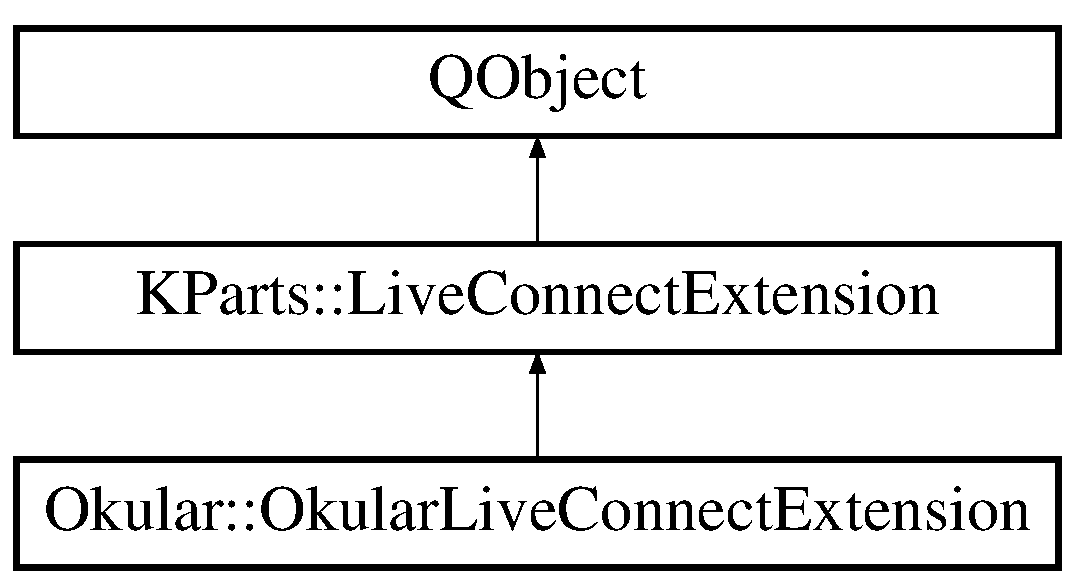
\includegraphics[height=3.000000cm]{classKParts_1_1LiveConnectExtension}
\end{center}
\end{figure}
\subsection*{Public Types}
\begin{DoxyCompactItemize}
\item 
enum \hyperlink{classKParts_1_1LiveConnectExtension_a8dfff0d5feb20316c714179c9eda9a9c}{Type} \{ \\*
\hyperlink{classKParts_1_1LiveConnectExtension_a8dfff0d5feb20316c714179c9eda9a9ca862f2f5258607f30adbbe03395426c20}{Type\+Void} =0, 
\hyperlink{classKParts_1_1LiveConnectExtension_a8dfff0d5feb20316c714179c9eda9a9ca3fed8b3ab2f5490fd7e6c6fca8b4a14b}{Type\+Bool}, 
\hyperlink{classKParts_1_1LiveConnectExtension_a8dfff0d5feb20316c714179c9eda9a9ca9f107d1ffb0bab7084c2952c00cf7f79}{Type\+Function}, 
\hyperlink{classKParts_1_1LiveConnectExtension_a8dfff0d5feb20316c714179c9eda9a9cadd765f23d443e96389613f184e874987}{Type\+Number}, 
\\*
\hyperlink{classKParts_1_1LiveConnectExtension_a8dfff0d5feb20316c714179c9eda9a9cadc439c83b2bb144692429d76408cb5b7}{Type\+Object}, 
\hyperlink{classKParts_1_1LiveConnectExtension_a8dfff0d5feb20316c714179c9eda9a9ca2f39f6b5f442bd7909c8810770d3ca95}{Type\+String}
 \}
\item 
typedef \hyperlink{classQList}{Q\+List}$<$ \hyperlink{structQPair}{Q\+Pair}$<$ \hyperlink{classKParts_1_1LiveConnectExtension_a8dfff0d5feb20316c714179c9eda9a9c}{Type}, \\*
Q\+String $>$ $>$ \hyperlink{classKParts_1_1LiveConnectExtension_a16a7a582605755e47eaab5b37e73d8cb}{Arg\+List}
\end{DoxyCompactItemize}
\subsection*{Public Member Functions}
\begin{DoxyCompactItemize}
\item 
\hyperlink{classKParts_1_1LiveConnectExtension_a11b7499199001f613246861dda90c101}{Live\+Connect\+Extension} (\hyperlink{classKParts_1_1ReadOnlyPart}{K\+Parts\+::\+Read\+Only\+Part} $\ast$parent)
\item 
virtual \hyperlink{classKParts_1_1LiveConnectExtension_aef598b47d0fc11d1323588c67928da7c}{$\sim$\+Live\+Connect\+Extension} ()
\item 
virtual bool \hyperlink{classKParts_1_1LiveConnectExtension_a91ddec0deaa49516ade1e86d8bbd3b90}{get} (const unsigned long objid, const Q\+String \&field, \hyperlink{classKParts_1_1LiveConnectExtension_a8dfff0d5feb20316c714179c9eda9a9c}{Type} \&type, unsigned long \&retobjid, Q\+String \&value)
\item 
virtual bool \hyperlink{classKParts_1_1LiveConnectExtension_a20088d732c9bf45abf31e9723b263e4f}{put} (const unsigned long objid, const Q\+String \&field, const Q\+String \&value)
\item 
virtual bool \hyperlink{classKParts_1_1LiveConnectExtension_ac925e087aa86e8e11c7616b8f03551a0}{call} (const unsigned long objid, const Q\+String \&func, const Q\+String\+List \&args, \hyperlink{classKParts_1_1LiveConnectExtension_a8dfff0d5feb20316c714179c9eda9a9c}{Type} \&type, unsigned long \&retobjid, Q\+String \&value)
\item 
virtual void \hyperlink{classKParts_1_1LiveConnectExtension_aceb4e2b994572baf1d87f78c7134c42a}{unregister} (const unsigned long objid)
\item 
void \hyperlink{classKParts_1_1LiveConnectExtension_a0cb4efb5b26992f31ae44f3d4a6ba2a1}{part\+Event} (const unsigned long objid, const Q\+String \&event, const \hyperlink{classKParts_1_1LiveConnectExtension_a16a7a582605755e47eaab5b37e73d8cb}{K\+Parts\+::\+Live\+Connect\+Extension\+::\+Arg\+List} \&args)
\end{DoxyCompactItemize}
\subsection*{Static Public Member Functions}
\begin{DoxyCompactItemize}
\item 
static \hyperlink{classKParts_1_1LiveConnectExtension}{Live\+Connect\+Extension} $\ast$ \hyperlink{classKParts_1_1LiveConnectExtension_acfe5c3014688d5b0efdc5a1534aacb49}{child\+Object} (Q\+Object $\ast$obj)
\end{DoxyCompactItemize}


\subsection{Detailed Description}
An extension class for Live\+Connect, i.\+e. a call from Java\+Script from a H\+T\+M\+L page which embeds this part. A part can have an object hierarchy by using objid as a reference to an object. 

Definition at line 765 of file browserextension.\+h.



\subsection{Member Typedef Documentation}
\hypertarget{classKParts_1_1LiveConnectExtension_a16a7a582605755e47eaab5b37e73d8cb}{\index{K\+Parts\+::\+Live\+Connect\+Extension@{K\+Parts\+::\+Live\+Connect\+Extension}!Arg\+List@{Arg\+List}}
\index{Arg\+List@{Arg\+List}!K\+Parts\+::\+Live\+Connect\+Extension@{K\+Parts\+::\+Live\+Connect\+Extension}}
\subsubsection[{Arg\+List}]{\setlength{\rightskip}{0pt plus 5cm}typedef {\bf Q\+List}$<${\bf Q\+Pair}$<${\bf Type}, Q\+String$>$ $>$ {\bf K\+Parts\+::\+Live\+Connect\+Extension\+::\+Arg\+List}}}\label{classKParts_1_1LiveConnectExtension_a16a7a582605755e47eaab5b37e73d8cb}


Definition at line 772 of file browserextension.\+h.



\subsection{Member Enumeration Documentation}
\hypertarget{classKParts_1_1LiveConnectExtension_a8dfff0d5feb20316c714179c9eda9a9c}{\index{K\+Parts\+::\+Live\+Connect\+Extension@{K\+Parts\+::\+Live\+Connect\+Extension}!Type@{Type}}
\index{Type@{Type}!K\+Parts\+::\+Live\+Connect\+Extension@{K\+Parts\+::\+Live\+Connect\+Extension}}
\subsubsection[{Type}]{\setlength{\rightskip}{0pt plus 5cm}enum {\bf K\+Parts\+::\+Live\+Connect\+Extension\+::\+Type}}}\label{classKParts_1_1LiveConnectExtension_a8dfff0d5feb20316c714179c9eda9a9c}
\begin{Desc}
\item[Enumerator]\par
\begin{description}
\index{Type\+Void@{Type\+Void}!K\+Parts\+::\+Live\+Connect\+Extension@{K\+Parts\+::\+Live\+Connect\+Extension}}\index{K\+Parts\+::\+Live\+Connect\+Extension@{K\+Parts\+::\+Live\+Connect\+Extension}!Type\+Void@{Type\+Void}}\item[{\em 
\hypertarget{classKParts_1_1LiveConnectExtension_a8dfff0d5feb20316c714179c9eda9a9ca862f2f5258607f30adbbe03395426c20}{Type\+Void}\label{classKParts_1_1LiveConnectExtension_a8dfff0d5feb20316c714179c9eda9a9ca862f2f5258607f30adbbe03395426c20}
}]\index{Type\+Bool@{Type\+Bool}!K\+Parts\+::\+Live\+Connect\+Extension@{K\+Parts\+::\+Live\+Connect\+Extension}}\index{K\+Parts\+::\+Live\+Connect\+Extension@{K\+Parts\+::\+Live\+Connect\+Extension}!Type\+Bool@{Type\+Bool}}\item[{\em 
\hypertarget{classKParts_1_1LiveConnectExtension_a8dfff0d5feb20316c714179c9eda9a9ca3fed8b3ab2f5490fd7e6c6fca8b4a14b}{Type\+Bool}\label{classKParts_1_1LiveConnectExtension_a8dfff0d5feb20316c714179c9eda9a9ca3fed8b3ab2f5490fd7e6c6fca8b4a14b}
}]\index{Type\+Function@{Type\+Function}!K\+Parts\+::\+Live\+Connect\+Extension@{K\+Parts\+::\+Live\+Connect\+Extension}}\index{K\+Parts\+::\+Live\+Connect\+Extension@{K\+Parts\+::\+Live\+Connect\+Extension}!Type\+Function@{Type\+Function}}\item[{\em 
\hypertarget{classKParts_1_1LiveConnectExtension_a8dfff0d5feb20316c714179c9eda9a9ca9f107d1ffb0bab7084c2952c00cf7f79}{Type\+Function}\label{classKParts_1_1LiveConnectExtension_a8dfff0d5feb20316c714179c9eda9a9ca9f107d1ffb0bab7084c2952c00cf7f79}
}]\index{Type\+Number@{Type\+Number}!K\+Parts\+::\+Live\+Connect\+Extension@{K\+Parts\+::\+Live\+Connect\+Extension}}\index{K\+Parts\+::\+Live\+Connect\+Extension@{K\+Parts\+::\+Live\+Connect\+Extension}!Type\+Number@{Type\+Number}}\item[{\em 
\hypertarget{classKParts_1_1LiveConnectExtension_a8dfff0d5feb20316c714179c9eda9a9cadd765f23d443e96389613f184e874987}{Type\+Number}\label{classKParts_1_1LiveConnectExtension_a8dfff0d5feb20316c714179c9eda9a9cadd765f23d443e96389613f184e874987}
}]\index{Type\+Object@{Type\+Object}!K\+Parts\+::\+Live\+Connect\+Extension@{K\+Parts\+::\+Live\+Connect\+Extension}}\index{K\+Parts\+::\+Live\+Connect\+Extension@{K\+Parts\+::\+Live\+Connect\+Extension}!Type\+Object@{Type\+Object}}\item[{\em 
\hypertarget{classKParts_1_1LiveConnectExtension_a8dfff0d5feb20316c714179c9eda9a9cadc439c83b2bb144692429d76408cb5b7}{Type\+Object}\label{classKParts_1_1LiveConnectExtension_a8dfff0d5feb20316c714179c9eda9a9cadc439c83b2bb144692429d76408cb5b7}
}]\index{Type\+String@{Type\+String}!K\+Parts\+::\+Live\+Connect\+Extension@{K\+Parts\+::\+Live\+Connect\+Extension}}\index{K\+Parts\+::\+Live\+Connect\+Extension@{K\+Parts\+::\+Live\+Connect\+Extension}!Type\+String@{Type\+String}}\item[{\em 
\hypertarget{classKParts_1_1LiveConnectExtension_a8dfff0d5feb20316c714179c9eda9a9ca2f39f6b5f442bd7909c8810770d3ca95}{Type\+String}\label{classKParts_1_1LiveConnectExtension_a8dfff0d5feb20316c714179c9eda9a9ca2f39f6b5f442bd7909c8810770d3ca95}
}]\end{description}
\end{Desc}


Definition at line 769 of file browserextension.\+h.


\begin{DoxyCode}
769             \{
770       \hyperlink{classKParts_1_1LiveConnectExtension_a8dfff0d5feb20316c714179c9eda9a9ca862f2f5258607f30adbbe03395426c20}{TypeVoid}=0, \hyperlink{classKParts_1_1LiveConnectExtension_a8dfff0d5feb20316c714179c9eda9a9ca3fed8b3ab2f5490fd7e6c6fca8b4a14b}{TypeBool}, \hyperlink{classKParts_1_1LiveConnectExtension_a8dfff0d5feb20316c714179c9eda9a9ca9f107d1ffb0bab7084c2952c00cf7f79}{TypeFunction}, \hyperlink{classKParts_1_1LiveConnectExtension_a8dfff0d5feb20316c714179c9eda9a9cadd765f23d443e96389613f184e874987}{TypeNumber}, 
      \hyperlink{classKParts_1_1LiveConnectExtension_a8dfff0d5feb20316c714179c9eda9a9cadc439c83b2bb144692429d76408cb5b7}{TypeObject}, \hyperlink{classKParts_1_1LiveConnectExtension_a8dfff0d5feb20316c714179c9eda9a9ca2f39f6b5f442bd7909c8810770d3ca95}{TypeString}
771   \};
\end{DoxyCode}


\subsection{Constructor \& Destructor Documentation}
\hypertarget{classKParts_1_1LiveConnectExtension_a11b7499199001f613246861dda90c101}{\index{K\+Parts\+::\+Live\+Connect\+Extension@{K\+Parts\+::\+Live\+Connect\+Extension}!Live\+Connect\+Extension@{Live\+Connect\+Extension}}
\index{Live\+Connect\+Extension@{Live\+Connect\+Extension}!K\+Parts\+::\+Live\+Connect\+Extension@{K\+Parts\+::\+Live\+Connect\+Extension}}
\subsubsection[{Live\+Connect\+Extension}]{\setlength{\rightskip}{0pt plus 5cm}K\+Parts\+::\+Live\+Connect\+Extension\+::\+Live\+Connect\+Extension (
\begin{DoxyParamCaption}
\item[{{\bf K\+Parts\+::\+Read\+Only\+Part} $\ast$}]{parent}
\end{DoxyParamCaption}
)}}\label{classKParts_1_1LiveConnectExtension_a11b7499199001f613246861dda90c101}
\hypertarget{classKParts_1_1LiveConnectExtension_aef598b47d0fc11d1323588c67928da7c}{\index{K\+Parts\+::\+Live\+Connect\+Extension@{K\+Parts\+::\+Live\+Connect\+Extension}!````~Live\+Connect\+Extension@{$\sim$\+Live\+Connect\+Extension}}
\index{````~Live\+Connect\+Extension@{$\sim$\+Live\+Connect\+Extension}!K\+Parts\+::\+Live\+Connect\+Extension@{K\+Parts\+::\+Live\+Connect\+Extension}}
\subsubsection[{$\sim$\+Live\+Connect\+Extension}]{\setlength{\rightskip}{0pt plus 5cm}virtual K\+Parts\+::\+Live\+Connect\+Extension\+::$\sim$\+Live\+Connect\+Extension (
\begin{DoxyParamCaption}
{}
\end{DoxyParamCaption}
)\hspace{0.3cm}{\ttfamily [virtual]}}}\label{classKParts_1_1LiveConnectExtension_aef598b47d0fc11d1323588c67928da7c}


\subsection{Member Function Documentation}
\hypertarget{classKParts_1_1LiveConnectExtension_ac925e087aa86e8e11c7616b8f03551a0}{\index{K\+Parts\+::\+Live\+Connect\+Extension@{K\+Parts\+::\+Live\+Connect\+Extension}!call@{call}}
\index{call@{call}!K\+Parts\+::\+Live\+Connect\+Extension@{K\+Parts\+::\+Live\+Connect\+Extension}}
\subsubsection[{call}]{\setlength{\rightskip}{0pt plus 5cm}virtual bool K\+Parts\+::\+Live\+Connect\+Extension\+::call (
\begin{DoxyParamCaption}
\item[{const unsigned long}]{objid, }
\item[{const Q\+String \&}]{func, }
\item[{const Q\+String\+List \&}]{args, }
\item[{{\bf Type} \&}]{type, }
\item[{unsigned long \&}]{retobjid, }
\item[{Q\+String \&}]{value}
\end{DoxyParamCaption}
)\hspace{0.3cm}{\ttfamily [virtual]}}}\label{classKParts_1_1LiveConnectExtension_ac925e087aa86e8e11c7616b8f03551a0}
calls a function of objid, return true on success 

Reimplemented in \hyperlink{classOkular_1_1OkularLiveConnectExtension_a1db71ccc9e59e46203cd7cd9eccd6870}{Okular\+::\+Okular\+Live\+Connect\+Extension}.

\hypertarget{classKParts_1_1LiveConnectExtension_acfe5c3014688d5b0efdc5a1534aacb49}{\index{K\+Parts\+::\+Live\+Connect\+Extension@{K\+Parts\+::\+Live\+Connect\+Extension}!child\+Object@{child\+Object}}
\index{child\+Object@{child\+Object}!K\+Parts\+::\+Live\+Connect\+Extension@{K\+Parts\+::\+Live\+Connect\+Extension}}
\subsubsection[{child\+Object}]{\setlength{\rightskip}{0pt plus 5cm}static {\bf Live\+Connect\+Extension}$\ast$ K\+Parts\+::\+Live\+Connect\+Extension\+::child\+Object (
\begin{DoxyParamCaption}
\item[{Q\+Object $\ast$}]{obj}
\end{DoxyParamCaption}
)\hspace{0.3cm}{\ttfamily [static]}}}\label{classKParts_1_1LiveConnectExtension_acfe5c3014688d5b0efdc5a1534aacb49}
\hypertarget{classKParts_1_1LiveConnectExtension_a91ddec0deaa49516ade1e86d8bbd3b90}{\index{K\+Parts\+::\+Live\+Connect\+Extension@{K\+Parts\+::\+Live\+Connect\+Extension}!get@{get}}
\index{get@{get}!K\+Parts\+::\+Live\+Connect\+Extension@{K\+Parts\+::\+Live\+Connect\+Extension}}
\subsubsection[{get}]{\setlength{\rightskip}{0pt plus 5cm}virtual bool K\+Parts\+::\+Live\+Connect\+Extension\+::get (
\begin{DoxyParamCaption}
\item[{const unsigned long}]{objid, }
\item[{const Q\+String \&}]{field, }
\item[{{\bf Type} \&}]{type, }
\item[{unsigned long \&}]{retobjid, }
\item[{Q\+String \&}]{value}
\end{DoxyParamCaption}
)\hspace{0.3cm}{\ttfamily [virtual]}}}\label{classKParts_1_1LiveConnectExtension_a91ddec0deaa49516ade1e86d8bbd3b90}
get a field value from objid, return true on success 

Reimplemented in \hyperlink{classOkular_1_1OkularLiveConnectExtension_ad0b24f4bdb9c4e2c010a83677ded3f69}{Okular\+::\+Okular\+Live\+Connect\+Extension}.

\hypertarget{classKParts_1_1LiveConnectExtension_a0cb4efb5b26992f31ae44f3d4a6ba2a1}{\index{K\+Parts\+::\+Live\+Connect\+Extension@{K\+Parts\+::\+Live\+Connect\+Extension}!part\+Event@{part\+Event}}
\index{part\+Event@{part\+Event}!K\+Parts\+::\+Live\+Connect\+Extension@{K\+Parts\+::\+Live\+Connect\+Extension}}
\subsubsection[{part\+Event}]{\setlength{\rightskip}{0pt plus 5cm}void K\+Parts\+::\+Live\+Connect\+Extension\+::part\+Event (
\begin{DoxyParamCaption}
\item[{const unsigned long}]{objid, }
\item[{const Q\+String \&}]{event, }
\item[{const {\bf K\+Parts\+::\+Live\+Connect\+Extension\+::\+Arg\+List} \&}]{args}
\end{DoxyParamCaption}
)}}\label{classKParts_1_1LiveConnectExtension_a0cb4efb5b26992f31ae44f3d4a6ba2a1}
notify a event from the part of object objid \hypertarget{classKParts_1_1LiveConnectExtension_a20088d732c9bf45abf31e9723b263e4f}{\index{K\+Parts\+::\+Live\+Connect\+Extension@{K\+Parts\+::\+Live\+Connect\+Extension}!put@{put}}
\index{put@{put}!K\+Parts\+::\+Live\+Connect\+Extension@{K\+Parts\+::\+Live\+Connect\+Extension}}
\subsubsection[{put}]{\setlength{\rightskip}{0pt plus 5cm}virtual bool K\+Parts\+::\+Live\+Connect\+Extension\+::put (
\begin{DoxyParamCaption}
\item[{const unsigned long}]{objid, }
\item[{const Q\+String \&}]{field, }
\item[{const Q\+String \&}]{value}
\end{DoxyParamCaption}
)\hspace{0.3cm}{\ttfamily [virtual]}}}\label{classKParts_1_1LiveConnectExtension_a20088d732c9bf45abf31e9723b263e4f}
put a field value in objid, return true on success 

Reimplemented in \hyperlink{classOkular_1_1OkularLiveConnectExtension_a694218a47c9f7fa0658fea86478b7e12}{Okular\+::\+Okular\+Live\+Connect\+Extension}.

\hypertarget{classKParts_1_1LiveConnectExtension_aceb4e2b994572baf1d87f78c7134c42a}{\index{K\+Parts\+::\+Live\+Connect\+Extension@{K\+Parts\+::\+Live\+Connect\+Extension}!unregister@{unregister}}
\index{unregister@{unregister}!K\+Parts\+::\+Live\+Connect\+Extension@{K\+Parts\+::\+Live\+Connect\+Extension}}
\subsubsection[{unregister}]{\setlength{\rightskip}{0pt plus 5cm}virtual void K\+Parts\+::\+Live\+Connect\+Extension\+::unregister (
\begin{DoxyParamCaption}
\item[{const unsigned long}]{objid}
\end{DoxyParamCaption}
)\hspace{0.3cm}{\ttfamily [virtual]}}}\label{classKParts_1_1LiveConnectExtension_aceb4e2b994572baf1d87f78c7134c42a}
notifies the part that there is no reference anymore to objid 

The documentation for this class was generated from the following file\+:\begin{DoxyCompactItemize}
\item 
/usr/include/kparts/\hyperlink{browserextension_8h}{browserextension.\+h}\end{DoxyCompactItemize}

\hypertarget{classKParts_1_1MainWindow}{\section{K\+Parts\+:\+:Main\+Window Class Reference}
\label{classKParts_1_1MainWindow}\index{K\+Parts\+::\+Main\+Window@{K\+Parts\+::\+Main\+Window}}
}


{\ttfamily \#include $<$mainwindow.\+h$>$}

Inheritance diagram for K\+Parts\+:\+:Main\+Window\+:\begin{figure}[H]
\begin{center}
\leavevmode
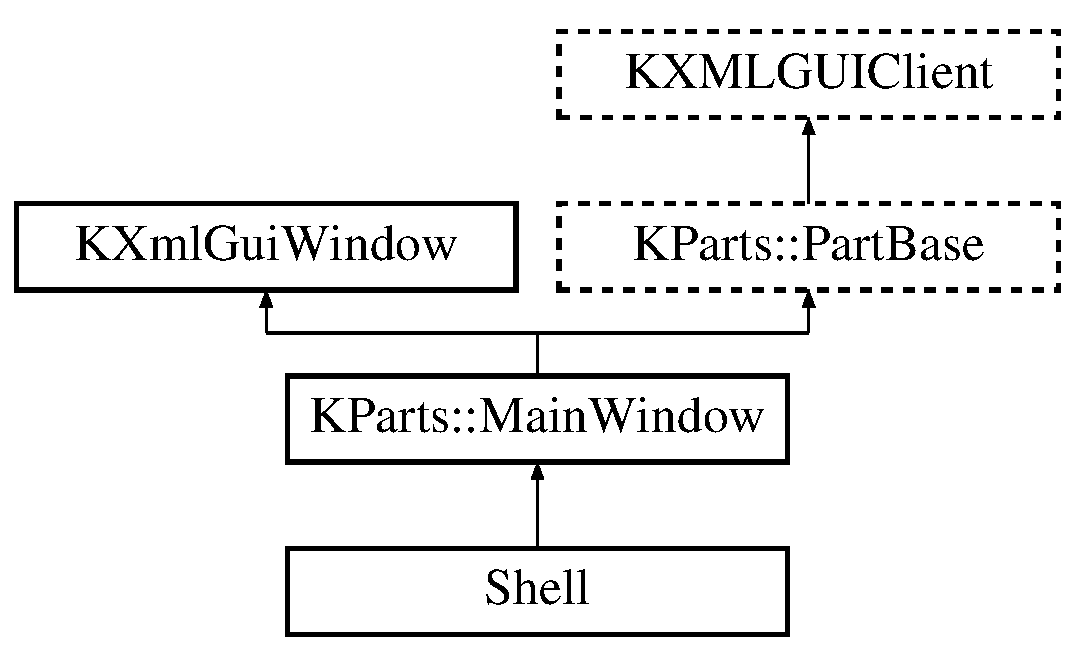
\includegraphics[height=4.000000cm]{classKParts_1_1MainWindow}
\end{center}
\end{figure}
\subsection*{Public Slots}
\begin{DoxyCompactItemize}
\item 
virtual void \hyperlink{classKParts_1_1MainWindow_a06a7c6c817f9b280804b0cabd28b3696}{configure\+Toolbars} ()
\end{DoxyCompactItemize}
\subsection*{Public Member Functions}
\begin{DoxyCompactItemize}
\item 
\hyperlink{classKParts_1_1MainWindow_a0691c70bec34e706409f019b91ca3173}{Main\+Window} (Q\+Widget $\ast$parent=0, Qt\+::\+Window\+Flags f=K\+D\+E\+\_\+\+D\+E\+F\+A\+U\+L\+T\+\_\+\+W\+I\+N\+D\+O\+W\+F\+L\+A\+G\+S)
\item 
K\+D\+E\+\_\+\+C\+O\+N\+S\+T\+R\+U\+C\+T\+O\+R\+\_\+\+D\+E\+P\+R\+E\+C\+A\+T\+E\+D \hyperlink{classKParts_1_1MainWindow_ad157c37ff711ecd0784569acb2582e07}{Main\+Window} (Q\+Widget $\ast$parent, const char $\ast$name=0, Qt\+::\+Window\+Flags f=K\+D\+E\+\_\+\+D\+E\+F\+A\+U\+L\+T\+\_\+\+W\+I\+N\+D\+O\+W\+F\+L\+A\+G\+S)
\item 
virtual \hyperlink{classKParts_1_1MainWindow_a475129f2af4142fbe3612ec61ee411ef}{$\sim$\+Main\+Window} ()
\end{DoxyCompactItemize}
\subsection*{Protected Slots}
\begin{DoxyCompactItemize}
\item 
void \hyperlink{classKParts_1_1MainWindow_ac9064b03c5b9c86676e107f0dd80693b}{create\+G\+U\+I} (\hyperlink{classKParts_1_1Part}{K\+Parts\+::\+Part} $\ast$part)
\item 
virtual void \hyperlink{classKParts_1_1MainWindow_a97b2f32ff0736617b5385274782dd26a}{slot\+Set\+Status\+Bar\+Text} (const Q\+String \&)
\item 
void \hyperlink{classKParts_1_1MainWindow_a7ee678f5096405ef023e49390013c0af}{save\+New\+Toolbar\+Config} ()
\end{DoxyCompactItemize}
\subsection*{Protected Member Functions}
\begin{DoxyCompactItemize}
\item 
virtual void \hyperlink{classKParts_1_1MainWindow_ac388eb6552660ee055c1d41e5f217553}{create\+Shell\+G\+U\+I} (bool create=true)
\end{DoxyCompactItemize}
\subsection*{Additional Inherited Members}


\subsection{Detailed Description}
A K\+Part-\/aware main window, whose user interface is described in X\+M\+L.

Inherit your main window from this class and don't forget to call set\+X\+M\+L\+File() in the inherited constructor.

It implements all internal interfaces in the case of a K\+Main\+Window as host\+: the builder and servant interface (for menu merging). 

Definition at line 46 of file mainwindow.\+h.



\subsection{Constructor \& Destructor Documentation}
\hypertarget{classKParts_1_1MainWindow_a0691c70bec34e706409f019b91ca3173}{\index{K\+Parts\+::\+Main\+Window@{K\+Parts\+::\+Main\+Window}!Main\+Window@{Main\+Window}}
\index{Main\+Window@{Main\+Window}!K\+Parts\+::\+Main\+Window@{K\+Parts\+::\+Main\+Window}}
\subsubsection[{Main\+Window}]{\setlength{\rightskip}{0pt plus 5cm}K\+Parts\+::\+Main\+Window\+::\+Main\+Window (
\begin{DoxyParamCaption}
\item[{Q\+Widget $\ast$}]{parent = {\ttfamily 0}, }
\item[{Qt\+::\+Window\+Flags}]{f = {\ttfamily KDE\+\_\+DEFAULT\+\_\+WINDOWFLAGS}}
\end{DoxyParamCaption}
)\hspace{0.3cm}{\ttfamily [explicit]}}}\label{classKParts_1_1MainWindow_a0691c70bec34e706409f019b91ca3173}
Constructor, same signature as K\+Main\+Window. \hypertarget{classKParts_1_1MainWindow_ad157c37ff711ecd0784569acb2582e07}{\index{K\+Parts\+::\+Main\+Window@{K\+Parts\+::\+Main\+Window}!Main\+Window@{Main\+Window}}
\index{Main\+Window@{Main\+Window}!K\+Parts\+::\+Main\+Window@{K\+Parts\+::\+Main\+Window}}
\subsubsection[{Main\+Window}]{\setlength{\rightskip}{0pt plus 5cm}K\+D\+E\+\_\+\+C\+O\+N\+S\+T\+R\+U\+C\+T\+O\+R\+\_\+\+D\+E\+P\+R\+E\+C\+A\+T\+E\+D K\+Parts\+::\+Main\+Window\+::\+Main\+Window (
\begin{DoxyParamCaption}
\item[{Q\+Widget $\ast$}]{parent, }
\item[{const char $\ast$}]{name = {\ttfamily 0}, }
\item[{Qt\+::\+Window\+Flags}]{f = {\ttfamily KDE\+\_\+DEFAULT\+\_\+WINDOWFLAGS}}
\end{DoxyParamCaption}
)\hspace{0.3cm}{\ttfamily [explicit]}}}\label{classKParts_1_1MainWindow_ad157c37ff711ecd0784569acb2582e07}
\begin{DoxyRefDesc}{Deprecated}
\item[\hyperlink{deprecated__deprecated000009}{Deprecated}], remove the name argument and use set\+Object\+Name instead \end{DoxyRefDesc}
\hypertarget{classKParts_1_1MainWindow_a475129f2af4142fbe3612ec61ee411ef}{\index{K\+Parts\+::\+Main\+Window@{K\+Parts\+::\+Main\+Window}!````~Main\+Window@{$\sim$\+Main\+Window}}
\index{````~Main\+Window@{$\sim$\+Main\+Window}!K\+Parts\+::\+Main\+Window@{K\+Parts\+::\+Main\+Window}}
\subsubsection[{$\sim$\+Main\+Window}]{\setlength{\rightskip}{0pt plus 5cm}virtual K\+Parts\+::\+Main\+Window\+::$\sim$\+Main\+Window (
\begin{DoxyParamCaption}
{}
\end{DoxyParamCaption}
)\hspace{0.3cm}{\ttfamily [virtual]}}}\label{classKParts_1_1MainWindow_a475129f2af4142fbe3612ec61ee411ef}
Destructor. 

\subsection{Member Function Documentation}
\hypertarget{classKParts_1_1MainWindow_a06a7c6c817f9b280804b0cabd28b3696}{\index{K\+Parts\+::\+Main\+Window@{K\+Parts\+::\+Main\+Window}!configure\+Toolbars@{configure\+Toolbars}}
\index{configure\+Toolbars@{configure\+Toolbars}!K\+Parts\+::\+Main\+Window@{K\+Parts\+::\+Main\+Window}}
\subsubsection[{configure\+Toolbars}]{\setlength{\rightskip}{0pt plus 5cm}virtual void K\+Parts\+::\+Main\+Window\+::configure\+Toolbars (
\begin{DoxyParamCaption}
{}
\end{DoxyParamCaption}
)\hspace{0.3cm}{\ttfamily [virtual]}, {\ttfamily [slot]}}}\label{classKParts_1_1MainWindow_a06a7c6c817f9b280804b0cabd28b3696}
\hypertarget{classKParts_1_1MainWindow_ac9064b03c5b9c86676e107f0dd80693b}{\index{K\+Parts\+::\+Main\+Window@{K\+Parts\+::\+Main\+Window}!create\+G\+U\+I@{create\+G\+U\+I}}
\index{create\+G\+U\+I@{create\+G\+U\+I}!K\+Parts\+::\+Main\+Window@{K\+Parts\+::\+Main\+Window}}
\subsubsection[{create\+G\+U\+I}]{\setlength{\rightskip}{0pt plus 5cm}void K\+Parts\+::\+Main\+Window\+::create\+G\+U\+I (
\begin{DoxyParamCaption}
\item[{{\bf K\+Parts\+::\+Part} $\ast$}]{part}
\end{DoxyParamCaption}
)\hspace{0.3cm}{\ttfamily [protected]}, {\ttfamily [slot]}}}\label{classKParts_1_1MainWindow_ac9064b03c5b9c86676e107f0dd80693b}
Create the G\+U\+I (by merging the host's and the active part's) You {\itshape must} call this in order to see any G\+U\+I being created.

In a main window with multiple parts being shown (e.\+g. as in Konqueror) you need to connect this slot to the K\+Part\+Manager\+::active\+Part\+Changed() signal


\begin{DoxyParams}{Parameters}
{\em part} & The active part (set to 0\+L if no part). \\
\hline
\end{DoxyParams}
\hypertarget{classKParts_1_1MainWindow_ac388eb6552660ee055c1d41e5f217553}{\index{K\+Parts\+::\+Main\+Window@{K\+Parts\+::\+Main\+Window}!create\+Shell\+G\+U\+I@{create\+Shell\+G\+U\+I}}
\index{create\+Shell\+G\+U\+I@{create\+Shell\+G\+U\+I}!K\+Parts\+::\+Main\+Window@{K\+Parts\+::\+Main\+Window}}
\subsubsection[{create\+Shell\+G\+U\+I}]{\setlength{\rightskip}{0pt plus 5cm}virtual void K\+Parts\+::\+Main\+Window\+::create\+Shell\+G\+U\+I (
\begin{DoxyParamCaption}
\item[{bool}]{create = {\ttfamily true}}
\end{DoxyParamCaption}
)\hspace{0.3cm}{\ttfamily [protected]}, {\ttfamily [virtual]}}}\label{classKParts_1_1MainWindow_ac388eb6552660ee055c1d41e5f217553}
\hypertarget{classKParts_1_1MainWindow_a7ee678f5096405ef023e49390013c0af}{\index{K\+Parts\+::\+Main\+Window@{K\+Parts\+::\+Main\+Window}!save\+New\+Toolbar\+Config@{save\+New\+Toolbar\+Config}}
\index{save\+New\+Toolbar\+Config@{save\+New\+Toolbar\+Config}!K\+Parts\+::\+Main\+Window@{K\+Parts\+::\+Main\+Window}}
\subsubsection[{save\+New\+Toolbar\+Config}]{\setlength{\rightskip}{0pt plus 5cm}void K\+Parts\+::\+Main\+Window\+::save\+New\+Toolbar\+Config (
\begin{DoxyParamCaption}
{}
\end{DoxyParamCaption}
)\hspace{0.3cm}{\ttfamily [protected]}, {\ttfamily [slot]}}}\label{classKParts_1_1MainWindow_a7ee678f5096405ef023e49390013c0af}
Rebuilds the G\+U\+I after K\+Edit\+Toolbar changed the toolbar layout. \begin{DoxySeeAlso}{See Also}
\hyperlink{classKParts_1_1MainWindow_a06a7c6c817f9b280804b0cabd28b3696}{configure\+Toolbars()} K\+D\+E4\+: make this virtual. (For now we rely on the fact that it's called as a slot, so the metaobject finds it here). 
\end{DoxySeeAlso}
\hypertarget{classKParts_1_1MainWindow_a97b2f32ff0736617b5385274782dd26a}{\index{K\+Parts\+::\+Main\+Window@{K\+Parts\+::\+Main\+Window}!slot\+Set\+Status\+Bar\+Text@{slot\+Set\+Status\+Bar\+Text}}
\index{slot\+Set\+Status\+Bar\+Text@{slot\+Set\+Status\+Bar\+Text}!K\+Parts\+::\+Main\+Window@{K\+Parts\+::\+Main\+Window}}
\subsubsection[{slot\+Set\+Status\+Bar\+Text}]{\setlength{\rightskip}{0pt plus 5cm}virtual void K\+Parts\+::\+Main\+Window\+::slot\+Set\+Status\+Bar\+Text (
\begin{DoxyParamCaption}
\item[{const Q\+String \&}]{}
\end{DoxyParamCaption}
)\hspace{0.3cm}{\ttfamily [protected]}, {\ttfamily [virtual]}, {\ttfamily [slot]}}}\label{classKParts_1_1MainWindow_a97b2f32ff0736617b5385274782dd26a}
Called when the active part wants to change the statusbar message Reimplement if your mainwindow has a complex statusbar (with several items) 

The documentation for this class was generated from the following file\+:\begin{DoxyCompactItemize}
\item 
/usr/include/kparts/\hyperlink{mainwindow_8h}{mainwindow.\+h}\end{DoxyCompactItemize}

\hypertarget{structKParts_1_1ScriptableExtension_1_1Null}{\section{\-K\-Parts\-:\-:\-Scriptable\-Extension\-:\-:\-Null \-Struct \-Reference}
\label{structKParts_1_1ScriptableExtension_1_1Null}\index{\-K\-Parts\-::\-Scriptable\-Extension\-::\-Null@{\-K\-Parts\-::\-Scriptable\-Extension\-::\-Null}}
}


\-Corresponds to 'null' in \-Java\-Script.  




{\ttfamily \#include $<$scriptableextension.\-h$>$}



\subsection{\-Detailed \-Description}
\-Corresponds to 'null' in \-Java\-Script. 

\-Definition at line 61 of file scriptableextension.\-h.



\-The documentation for this struct was generated from the following file\-:\begin{DoxyCompactItemize}
\item 
/usr/include/kparts/\hyperlink{scriptableextension_8h}{scriptableextension.\-h}\end{DoxyCompactItemize}

\hypertarget{structKParts_1_1ScriptableExtension_1_1Object}{\section{K\+Parts\+:\+:Scriptable\+Extension\+:\+:Object Struct Reference}
\label{structKParts_1_1ScriptableExtension_1_1Object}\index{K\+Parts\+::\+Scriptable\+Extension\+::\+Object@{K\+Parts\+::\+Scriptable\+Extension\+::\+Object}}
}


{\ttfamily \#include $<$scriptableextension.\+h$>$}

\subsection*{Public Member Functions}
\begin{DoxyCompactItemize}
\item 
\hyperlink{structKParts_1_1ScriptableExtension_1_1Object_ac328d8854e2e0ceec2b83544ed34e549}{Object} ()
\item 
\hyperlink{structKParts_1_1ScriptableExtension_1_1Object_a322cdc635a708b3e19fe61d576c3c865}{Object} (\hyperlink{classKParts_1_1ScriptableExtension}{Scriptable\+Extension} $\ast$o, quint64 id)
\item 
bool \hyperlink{structKParts_1_1ScriptableExtension_1_1Object_a9b11da1473dc4d6bedd85334b3c8f44b}{operator==} (const \hyperlink{structKParts_1_1ScriptableExtension_1_1Object}{Object} \&other) const 
\end{DoxyCompactItemize}
\subsection*{Public Attributes}
\begin{DoxyCompactItemize}
\item 
\hyperlink{classKParts_1_1ScriptableExtension}{Scriptable\+Extension} $\ast$ \hyperlink{structKParts_1_1ScriptableExtension_1_1Object_a2e2ad2aca3cec31e49e8393658a6997c}{owner}
\item 
quint64 \hyperlink{structKParts_1_1ScriptableExtension_1_1Object_a884270fd3423ea40ec2920cb15c9bd15}{obj\+Id}
\end{DoxyCompactItemize}


\subsection{Detailed Description}
Objects are abstracted away as a pair of the \hyperlink{classKParts_1_1ScriptableExtension}{Scriptable\+Extension} the performs operations on it, and an implementation-\/specific Id, which gets passed to the extension's methods.

Objects are reference-\/counted, with the following protocol\+: 1) Return values from methods, \hyperlink{classKParts_1_1ScriptableExtension_a2e74d0dce5db4528968dc545a73e22d6}{root\+Object()}, \hyperlink{classKParts_1_1ScriptableExtension_a1654d1f14b8f3184c4a2c4e382826aee}{enclosing\+Object()}, and \hyperlink{classKParts_1_1ScriptableExtension_a90f5b0047ddb0b78096cab68a40c6326}{get()} are already acquired by the producer, so the consumer should release them when done. 2) During a call, the caller guarantees that all the arguments will be live for the calls duration, but the callee must acquire them if it stores it for longer than that.

\begin{DoxySeeAlso}{See Also}
\hyperlink{classKParts_1_1ScriptableExtension_aa9d21d12e60a00fa4adb0a3db0f52cad}{acquire}, \hyperlink{classKParts_1_1ScriptableExtension_a048b779677ccf0e99e90b101281d31bc}{acquire\+Value}, \hyperlink{classKParts_1_1ScriptableExtension_a1a06fcb64081a052d29baae2376c371b}{release}, \hyperlink{classKParts_1_1ScriptableExtension_a45af0ab34d52c57452910b6161922c3c}{release\+Value} 
\end{DoxySeeAlso}


Definition at line 91 of file scriptableextension.\+h.



\subsection{Constructor \& Destructor Documentation}
\hypertarget{structKParts_1_1ScriptableExtension_1_1Object_ac328d8854e2e0ceec2b83544ed34e549}{\index{K\+Parts\+::\+Scriptable\+Extension\+::\+Object@{K\+Parts\+::\+Scriptable\+Extension\+::\+Object}!Object@{Object}}
\index{Object@{Object}!K\+Parts\+::\+Scriptable\+Extension\+::\+Object@{K\+Parts\+::\+Scriptable\+Extension\+::\+Object}}
\subsubsection[{Object}]{\setlength{\rightskip}{0pt plus 5cm}K\+Parts\+::\+Scriptable\+Extension\+::\+Object\+::\+Object (
\begin{DoxyParamCaption}
{}
\end{DoxyParamCaption}
)\hspace{0.3cm}{\ttfamily [inline]}}}\label{structKParts_1_1ScriptableExtension_1_1Object_ac328d8854e2e0ceec2b83544ed34e549}


Definition at line 95 of file scriptableextension.\+h.


\begin{DoxyCode}
95 : \hyperlink{structKParts_1_1ScriptableExtension_1_1Object_a2e2ad2aca3cec31e49e8393658a6997c}{owner}(0), \hyperlink{structKParts_1_1ScriptableExtension_1_1Object_a884270fd3423ea40ec2920cb15c9bd15}{objId}(0) \{\}
\end{DoxyCode}
\hypertarget{structKParts_1_1ScriptableExtension_1_1Object_a322cdc635a708b3e19fe61d576c3c865}{\index{K\+Parts\+::\+Scriptable\+Extension\+::\+Object@{K\+Parts\+::\+Scriptable\+Extension\+::\+Object}!Object@{Object}}
\index{Object@{Object}!K\+Parts\+::\+Scriptable\+Extension\+::\+Object@{K\+Parts\+::\+Scriptable\+Extension\+::\+Object}}
\subsubsection[{Object}]{\setlength{\rightskip}{0pt plus 5cm}K\+Parts\+::\+Scriptable\+Extension\+::\+Object\+::\+Object (
\begin{DoxyParamCaption}
\item[{{\bf Scriptable\+Extension} $\ast$}]{o, }
\item[{quint64}]{id}
\end{DoxyParamCaption}
)\hspace{0.3cm}{\ttfamily [inline]}}}\label{structKParts_1_1ScriptableExtension_1_1Object_a322cdc635a708b3e19fe61d576c3c865}


Definition at line 96 of file scriptableextension.\+h.


\begin{DoxyCode}
96 : \hyperlink{structKParts_1_1ScriptableExtension_1_1Object_a2e2ad2aca3cec31e49e8393658a6997c}{owner}(o), \hyperlink{structKParts_1_1ScriptableExtension_1_1Object_a884270fd3423ea40ec2920cb15c9bd15}{objId}(\textcolor{keywordtype}{id}) \{\}
\end{DoxyCode}


\subsection{Member Function Documentation}
\hypertarget{structKParts_1_1ScriptableExtension_1_1Object_a9b11da1473dc4d6bedd85334b3c8f44b}{\index{K\+Parts\+::\+Scriptable\+Extension\+::\+Object@{K\+Parts\+::\+Scriptable\+Extension\+::\+Object}!operator==@{operator==}}
\index{operator==@{operator==}!K\+Parts\+::\+Scriptable\+Extension\+::\+Object@{K\+Parts\+::\+Scriptable\+Extension\+::\+Object}}
\subsubsection[{operator==}]{\setlength{\rightskip}{0pt plus 5cm}bool K\+Parts\+::\+Scriptable\+Extension\+::\+Object\+::operator== (
\begin{DoxyParamCaption}
\item[{const {\bf Object} \&}]{other}
\end{DoxyParamCaption}
) const\hspace{0.3cm}{\ttfamily [inline]}}}\label{structKParts_1_1ScriptableExtension_1_1Object_a9b11da1473dc4d6bedd85334b3c8f44b}


Definition at line 97 of file scriptableextension.\+h.


\begin{DoxyCode}
97 \{ \textcolor{keywordflow}{return} \hyperlink{structKParts_1_1ScriptableExtension_1_1Object_a2e2ad2aca3cec31e49e8393658a6997c}{owner} == other.owner && \hyperlink{structKParts_1_1ScriptableExtension_1_1Object_a884270fd3423ea40ec2920cb15c9bd15}{objId} == other.objId; \}
\end{DoxyCode}


\subsection{Member Data Documentation}
\hypertarget{structKParts_1_1ScriptableExtension_1_1Object_a884270fd3423ea40ec2920cb15c9bd15}{\index{K\+Parts\+::\+Scriptable\+Extension\+::\+Object@{K\+Parts\+::\+Scriptable\+Extension\+::\+Object}!obj\+Id@{obj\+Id}}
\index{obj\+Id@{obj\+Id}!K\+Parts\+::\+Scriptable\+Extension\+::\+Object@{K\+Parts\+::\+Scriptable\+Extension\+::\+Object}}
\subsubsection[{obj\+Id}]{\setlength{\rightskip}{0pt plus 5cm}quint64 K\+Parts\+::\+Scriptable\+Extension\+::\+Object\+::obj\+Id}}\label{structKParts_1_1ScriptableExtension_1_1Object_a884270fd3423ea40ec2920cb15c9bd15}


Definition at line 93 of file scriptableextension.\+h.

\hypertarget{structKParts_1_1ScriptableExtension_1_1Object_a2e2ad2aca3cec31e49e8393658a6997c}{\index{K\+Parts\+::\+Scriptable\+Extension\+::\+Object@{K\+Parts\+::\+Scriptable\+Extension\+::\+Object}!owner@{owner}}
\index{owner@{owner}!K\+Parts\+::\+Scriptable\+Extension\+::\+Object@{K\+Parts\+::\+Scriptable\+Extension\+::\+Object}}
\subsubsection[{owner}]{\setlength{\rightskip}{0pt plus 5cm}{\bf Scriptable\+Extension}$\ast$ K\+Parts\+::\+Scriptable\+Extension\+::\+Object\+::owner}}\label{structKParts_1_1ScriptableExtension_1_1Object_a2e2ad2aca3cec31e49e8393658a6997c}


Definition at line 92 of file scriptableextension.\+h.



The documentation for this struct was generated from the following file\+:\begin{DoxyCompactItemize}
\item 
/usr/include/kparts/\hyperlink{scriptableextension_8h}{scriptableextension.\+h}\end{DoxyCompactItemize}

\hypertarget{classKParts_1_1OpenUrlArguments}{\section{\-K\-Parts\-:\-:\-Open\-Url\-Arguments \-Class \-Reference}
\label{classKParts_1_1OpenUrlArguments}\index{\-K\-Parts\-::\-Open\-Url\-Arguments@{\-K\-Parts\-::\-Open\-Url\-Arguments}}
}


{\ttfamily \#include $<$part.\-h$>$}

\subsection*{\-Public \-Member \-Functions}
\begin{DoxyCompactItemize}
\item 
\hyperlink{classKParts_1_1OpenUrlArguments_af4c1ee81217691a1dc9c7db9ba7d59f8}{\-Open\-Url\-Arguments} ()
\item 
\hyperlink{classKParts_1_1OpenUrlArguments_ac6d97bc2c3d8f926bd163b3a35bd5809}{\-Open\-Url\-Arguments} (const \hyperlink{classKParts_1_1OpenUrlArguments}{\-Open\-Url\-Arguments} \&other)
\item 
\hyperlink{classKParts_1_1OpenUrlArguments}{\-Open\-Url\-Arguments} \& \hyperlink{classKParts_1_1OpenUrlArguments_a17e55b23d031666e50cc96aae65233f3}{operator=} (const \hyperlink{classKParts_1_1OpenUrlArguments}{\-Open\-Url\-Arguments} \&other)
\item 
\hyperlink{classKParts_1_1OpenUrlArguments_a667623f26093523412bd9060b423971d}{$\sim$\-Open\-Url\-Arguments} ()
\item 
bool \hyperlink{classKParts_1_1OpenUrlArguments_a75c903644fed82bc1982cededcb1c05a}{reload} () const 
\item 
void \hyperlink{classKParts_1_1OpenUrlArguments_a2b9d7ac959db074ef06697de8f4e7a14}{set\-Reload} (bool b)
\item 
int \hyperlink{classKParts_1_1OpenUrlArguments_a3eb562ffb04cc93b0a5aa0e385058aa3}{x\-Offset} () const 
\item 
void \hyperlink{classKParts_1_1OpenUrlArguments_a2429db3ff60f2cca3aac4d3e9c7cde7b}{set\-X\-Offset} (int x)
\item 
int \hyperlink{classKParts_1_1OpenUrlArguments_a29dbdad63be6e6904d5fd2c9fd9cd38b}{y\-Offset} () const 
\item 
void \hyperlink{classKParts_1_1OpenUrlArguments_a19d0a9e25a2bbe4cd0d7c255bfa8441c}{set\-Y\-Offset} (int y)
\item 
\-Q\-String \hyperlink{classKParts_1_1OpenUrlArguments_aaddc679e216a0ce1a20983c0134675c5}{mime\-Type} () const 
\item 
void \hyperlink{classKParts_1_1OpenUrlArguments_aa3c7601bb5f1ecfa1ed23009f7dfdc87}{set\-Mime\-Type} (const \-Q\-String \&mime)
\item 
bool \hyperlink{classKParts_1_1OpenUrlArguments_ab581f9d940912f8e8967f34c56cd2e29}{action\-Requested\-By\-User} () const 
\item 
void \hyperlink{classKParts_1_1OpenUrlArguments_ac3e9c56a054c7d5fb882e5724f713041}{set\-Action\-Requested\-By\-User} (bool user\-Requested)
\item 
\-Q\-Map$<$ \-Q\-String, \-Q\-String $>$ \& \hyperlink{classKParts_1_1OpenUrlArguments_a8c85d3cfe28606c6101f382158468d72}{meta\-Data} ()
\item 
const \-Q\-Map$<$ \-Q\-String, \-Q\-String $>$ \& \hyperlink{classKParts_1_1OpenUrlArguments_abf11199bbcb7496af97a0058c1a2c7f6}{meta\-Data} () const 
\end{DoxyCompactItemize}


\subsection{\-Detailed \-Description}
\hyperlink{classKParts_1_1OpenUrlArguments}{\-Open\-Url\-Arguments} is the set of arguments that specify how a \-U\-R\-L should be opened by \hyperlink{classKParts_1_1ReadOnlyPart_a1ff41b28f8da57ccc380e0c092a50c0c}{\-K\-Parts\-::\-Read\-Only\-Part\-::open\-Url()}.

\-For instance \hyperlink{classKParts_1_1OpenUrlArguments_a75c903644fed82bc1982cededcb1c05a}{reload()} indicates that the url should be loaded from the network even if it matches the current url of the part.

\-All setter methods in this class are for the class that calls open\-Url (usually the hosting application), all the getter methods are for the part. 

\-Definition at line 404 of file part.\-h.



\subsection{\-Constructor \& \-Destructor \-Documentation}
\hypertarget{classKParts_1_1OpenUrlArguments_af4c1ee81217691a1dc9c7db9ba7d59f8}{\index{\-K\-Parts\-::\-Open\-Url\-Arguments@{\-K\-Parts\-::\-Open\-Url\-Arguments}!\-Open\-Url\-Arguments@{\-Open\-Url\-Arguments}}
\index{\-Open\-Url\-Arguments@{\-Open\-Url\-Arguments}!KParts::OpenUrlArguments@{\-K\-Parts\-::\-Open\-Url\-Arguments}}
\subsubsection[{\-Open\-Url\-Arguments}]{\setlength{\rightskip}{0pt plus 5cm}{\bf \-K\-Parts\-::\-Open\-Url\-Arguments\-::\-Open\-Url\-Arguments} (
\begin{DoxyParamCaption}
{}
\end{DoxyParamCaption}
)}}\label{classKParts_1_1OpenUrlArguments_af4c1ee81217691a1dc9c7db9ba7d59f8}
\hypertarget{classKParts_1_1OpenUrlArguments_ac6d97bc2c3d8f926bd163b3a35bd5809}{\index{\-K\-Parts\-::\-Open\-Url\-Arguments@{\-K\-Parts\-::\-Open\-Url\-Arguments}!\-Open\-Url\-Arguments@{\-Open\-Url\-Arguments}}
\index{\-Open\-Url\-Arguments@{\-Open\-Url\-Arguments}!KParts::OpenUrlArguments@{\-K\-Parts\-::\-Open\-Url\-Arguments}}
\subsubsection[{\-Open\-Url\-Arguments}]{\setlength{\rightskip}{0pt plus 5cm}{\bf \-K\-Parts\-::\-Open\-Url\-Arguments\-::\-Open\-Url\-Arguments} (
\begin{DoxyParamCaption}
\item[{const {\bf \-Open\-Url\-Arguments} \&}]{other}
\end{DoxyParamCaption}
)}}\label{classKParts_1_1OpenUrlArguments_ac6d97bc2c3d8f926bd163b3a35bd5809}
\hypertarget{classKParts_1_1OpenUrlArguments_a667623f26093523412bd9060b423971d}{\index{\-K\-Parts\-::\-Open\-Url\-Arguments@{\-K\-Parts\-::\-Open\-Url\-Arguments}!$\sim$\-Open\-Url\-Arguments@{$\sim$\-Open\-Url\-Arguments}}
\index{$\sim$\-Open\-Url\-Arguments@{$\sim$\-Open\-Url\-Arguments}!KParts::OpenUrlArguments@{\-K\-Parts\-::\-Open\-Url\-Arguments}}
\subsubsection[{$\sim$\-Open\-Url\-Arguments}]{\setlength{\rightskip}{0pt plus 5cm}{\bf \-K\-Parts\-::\-Open\-Url\-Arguments\-::$\sim$\-Open\-Url\-Arguments} (
\begin{DoxyParamCaption}
{}
\end{DoxyParamCaption}
)}}\label{classKParts_1_1OpenUrlArguments_a667623f26093523412bd9060b423971d}


\subsection{\-Member \-Function \-Documentation}
\hypertarget{classKParts_1_1OpenUrlArguments_ab581f9d940912f8e8967f34c56cd2e29}{\index{\-K\-Parts\-::\-Open\-Url\-Arguments@{\-K\-Parts\-::\-Open\-Url\-Arguments}!action\-Requested\-By\-User@{action\-Requested\-By\-User}}
\index{action\-Requested\-By\-User@{action\-Requested\-By\-User}!KParts::OpenUrlArguments@{\-K\-Parts\-::\-Open\-Url\-Arguments}}
\subsubsection[{action\-Requested\-By\-User}]{\setlength{\rightskip}{0pt plus 5cm}bool {\bf \-K\-Parts\-::\-Open\-Url\-Arguments\-::action\-Requested\-By\-User} (
\begin{DoxyParamCaption}
{}
\end{DoxyParamCaption}
) const}}\label{classKParts_1_1OpenUrlArguments_ab581f9d940912f8e8967f34c56cd2e29}
\-True if the user requested that the \-U\-R\-L be opened. \-False if the \-U\-R\-L should be opened due to an external event, like javascript popups or automatic redirections. \-This is true by default \begin{DoxySince}{\-Since}
4.\-1 
\end{DoxySince}
\hypertarget{classKParts_1_1OpenUrlArguments_a8c85d3cfe28606c6101f382158468d72}{\index{\-K\-Parts\-::\-Open\-Url\-Arguments@{\-K\-Parts\-::\-Open\-Url\-Arguments}!meta\-Data@{meta\-Data}}
\index{meta\-Data@{meta\-Data}!KParts::OpenUrlArguments@{\-K\-Parts\-::\-Open\-Url\-Arguments}}
\subsubsection[{meta\-Data}]{\setlength{\rightskip}{0pt plus 5cm}\-Q\-Map$<$\-Q\-String, \-Q\-String$>$\& {\bf \-K\-Parts\-::\-Open\-Url\-Arguments\-::meta\-Data} (
\begin{DoxyParamCaption}
{}
\end{DoxyParamCaption}
)}}\label{classKParts_1_1OpenUrlArguments_a8c85d3cfe28606c6101f382158468d72}
\-Meta-\/data to associate with the \hyperlink{namespaceKIO}{\-K\-I\-O} operation that will be used to open the \-U\-R\-L. \-This method can be used to add or retrieve metadata. \begin{DoxySeeAlso}{\-See also}
\-K\-I\-O\-::\-Transfer\-Job etc. 
\end{DoxySeeAlso}
\hypertarget{classKParts_1_1OpenUrlArguments_abf11199bbcb7496af97a0058c1a2c7f6}{\index{\-K\-Parts\-::\-Open\-Url\-Arguments@{\-K\-Parts\-::\-Open\-Url\-Arguments}!meta\-Data@{meta\-Data}}
\index{meta\-Data@{meta\-Data}!KParts::OpenUrlArguments@{\-K\-Parts\-::\-Open\-Url\-Arguments}}
\subsubsection[{meta\-Data}]{\setlength{\rightskip}{0pt plus 5cm}const \-Q\-Map$<$\-Q\-String, \-Q\-String$>$\& {\bf \-K\-Parts\-::\-Open\-Url\-Arguments\-::meta\-Data} (
\begin{DoxyParamCaption}
{}
\end{DoxyParamCaption}
) const}}\label{classKParts_1_1OpenUrlArguments_abf11199bbcb7496af97a0058c1a2c7f6}
\hypertarget{classKParts_1_1OpenUrlArguments_aaddc679e216a0ce1a20983c0134675c5}{\index{\-K\-Parts\-::\-Open\-Url\-Arguments@{\-K\-Parts\-::\-Open\-Url\-Arguments}!mime\-Type@{mime\-Type}}
\index{mime\-Type@{mime\-Type}!KParts::OpenUrlArguments@{\-K\-Parts\-::\-Open\-Url\-Arguments}}
\subsubsection[{mime\-Type}]{\setlength{\rightskip}{0pt plus 5cm}\-Q\-String {\bf \-K\-Parts\-::\-Open\-Url\-Arguments\-::mime\-Type} (
\begin{DoxyParamCaption}
{}
\end{DoxyParamCaption}
) const}}\label{classKParts_1_1OpenUrlArguments_aaddc679e216a0ce1a20983c0134675c5}
\-The mimetype to use when opening the url, when known by the calling application. \hypertarget{classKParts_1_1OpenUrlArguments_a17e55b23d031666e50cc96aae65233f3}{\index{\-K\-Parts\-::\-Open\-Url\-Arguments@{\-K\-Parts\-::\-Open\-Url\-Arguments}!operator=@{operator=}}
\index{operator=@{operator=}!KParts::OpenUrlArguments@{\-K\-Parts\-::\-Open\-Url\-Arguments}}
\subsubsection[{operator=}]{\setlength{\rightskip}{0pt plus 5cm}{\bf \-Open\-Url\-Arguments}\& \-K\-Parts\-::\-Open\-Url\-Arguments\-::operator= (
\begin{DoxyParamCaption}
\item[{const {\bf \-Open\-Url\-Arguments} \&}]{other}
\end{DoxyParamCaption}
)}}\label{classKParts_1_1OpenUrlArguments_a17e55b23d031666e50cc96aae65233f3}
\hypertarget{classKParts_1_1OpenUrlArguments_a75c903644fed82bc1982cededcb1c05a}{\index{\-K\-Parts\-::\-Open\-Url\-Arguments@{\-K\-Parts\-::\-Open\-Url\-Arguments}!reload@{reload}}
\index{reload@{reload}!KParts::OpenUrlArguments@{\-K\-Parts\-::\-Open\-Url\-Arguments}}
\subsubsection[{reload}]{\setlength{\rightskip}{0pt plus 5cm}bool {\bf \-K\-Parts\-::\-Open\-Url\-Arguments\-::reload} (
\begin{DoxyParamCaption}
{}
\end{DoxyParamCaption}
) const}}\label{classKParts_1_1OpenUrlArguments_a75c903644fed82bc1982cededcb1c05a}
\begin{DoxyReturn}{\-Returns}
true to indicate that the part should reload the \-U\-R\-L, i.\-e. the cache shouldn't be used (forced reload). 
\end{DoxyReturn}
\hypertarget{classKParts_1_1OpenUrlArguments_ac3e9c56a054c7d5fb882e5724f713041}{\index{\-K\-Parts\-::\-Open\-Url\-Arguments@{\-K\-Parts\-::\-Open\-Url\-Arguments}!set\-Action\-Requested\-By\-User@{set\-Action\-Requested\-By\-User}}
\index{set\-Action\-Requested\-By\-User@{set\-Action\-Requested\-By\-User}!KParts::OpenUrlArguments@{\-K\-Parts\-::\-Open\-Url\-Arguments}}
\subsubsection[{set\-Action\-Requested\-By\-User}]{\setlength{\rightskip}{0pt plus 5cm}void {\bf \-K\-Parts\-::\-Open\-Url\-Arguments\-::set\-Action\-Requested\-By\-User} (
\begin{DoxyParamCaption}
\item[{bool}]{user\-Requested}
\end{DoxyParamCaption}
)}}\label{classKParts_1_1OpenUrlArguments_ac3e9c56a054c7d5fb882e5724f713041}
\hypertarget{classKParts_1_1OpenUrlArguments_aa3c7601bb5f1ecfa1ed23009f7dfdc87}{\index{\-K\-Parts\-::\-Open\-Url\-Arguments@{\-K\-Parts\-::\-Open\-Url\-Arguments}!set\-Mime\-Type@{set\-Mime\-Type}}
\index{set\-Mime\-Type@{set\-Mime\-Type}!KParts::OpenUrlArguments@{\-K\-Parts\-::\-Open\-Url\-Arguments}}
\subsubsection[{set\-Mime\-Type}]{\setlength{\rightskip}{0pt plus 5cm}void {\bf \-K\-Parts\-::\-Open\-Url\-Arguments\-::set\-Mime\-Type} (
\begin{DoxyParamCaption}
\item[{const \-Q\-String \&}]{mime}
\end{DoxyParamCaption}
)}}\label{classKParts_1_1OpenUrlArguments_aa3c7601bb5f1ecfa1ed23009f7dfdc87}
\hypertarget{classKParts_1_1OpenUrlArguments_a2b9d7ac959db074ef06697de8f4e7a14}{\index{\-K\-Parts\-::\-Open\-Url\-Arguments@{\-K\-Parts\-::\-Open\-Url\-Arguments}!set\-Reload@{set\-Reload}}
\index{set\-Reload@{set\-Reload}!KParts::OpenUrlArguments@{\-K\-Parts\-::\-Open\-Url\-Arguments}}
\subsubsection[{set\-Reload}]{\setlength{\rightskip}{0pt plus 5cm}void {\bf \-K\-Parts\-::\-Open\-Url\-Arguments\-::set\-Reload} (
\begin{DoxyParamCaption}
\item[{bool}]{b}
\end{DoxyParamCaption}
)}}\label{classKParts_1_1OpenUrlArguments_a2b9d7ac959db074ef06697de8f4e7a14}
\-Indicates that the url should be loaded from the network even if it matches the current url of the part. \hypertarget{classKParts_1_1OpenUrlArguments_a2429db3ff60f2cca3aac4d3e9c7cde7b}{\index{\-K\-Parts\-::\-Open\-Url\-Arguments@{\-K\-Parts\-::\-Open\-Url\-Arguments}!set\-X\-Offset@{set\-X\-Offset}}
\index{set\-X\-Offset@{set\-X\-Offset}!KParts::OpenUrlArguments@{\-K\-Parts\-::\-Open\-Url\-Arguments}}
\subsubsection[{set\-X\-Offset}]{\setlength{\rightskip}{0pt plus 5cm}void {\bf \-K\-Parts\-::\-Open\-Url\-Arguments\-::set\-X\-Offset} (
\begin{DoxyParamCaption}
\item[{int}]{x}
\end{DoxyParamCaption}
)}}\label{classKParts_1_1OpenUrlArguments_a2429db3ff60f2cca3aac4d3e9c7cde7b}
\hypertarget{classKParts_1_1OpenUrlArguments_a19d0a9e25a2bbe4cd0d7c255bfa8441c}{\index{\-K\-Parts\-::\-Open\-Url\-Arguments@{\-K\-Parts\-::\-Open\-Url\-Arguments}!set\-Y\-Offset@{set\-Y\-Offset}}
\index{set\-Y\-Offset@{set\-Y\-Offset}!KParts::OpenUrlArguments@{\-K\-Parts\-::\-Open\-Url\-Arguments}}
\subsubsection[{set\-Y\-Offset}]{\setlength{\rightskip}{0pt plus 5cm}void {\bf \-K\-Parts\-::\-Open\-Url\-Arguments\-::set\-Y\-Offset} (
\begin{DoxyParamCaption}
\item[{int}]{y}
\end{DoxyParamCaption}
)}}\label{classKParts_1_1OpenUrlArguments_a19d0a9e25a2bbe4cd0d7c255bfa8441c}
\hypertarget{classKParts_1_1OpenUrlArguments_a3eb562ffb04cc93b0a5aa0e385058aa3}{\index{\-K\-Parts\-::\-Open\-Url\-Arguments@{\-K\-Parts\-::\-Open\-Url\-Arguments}!x\-Offset@{x\-Offset}}
\index{x\-Offset@{x\-Offset}!KParts::OpenUrlArguments@{\-K\-Parts\-::\-Open\-Url\-Arguments}}
\subsubsection[{x\-Offset}]{\setlength{\rightskip}{0pt plus 5cm}int {\bf \-K\-Parts\-::\-Open\-Url\-Arguments\-::x\-Offset} (
\begin{DoxyParamCaption}
{}
\end{DoxyParamCaption}
) const}}\label{classKParts_1_1OpenUrlArguments_a3eb562ffb04cc93b0a5aa0e385058aa3}
x\-Offset is the horizontal scrolling of the part's widget (in case it's a scrollview). \-This is saved into the history and restored when going back in the history. \hypertarget{classKParts_1_1OpenUrlArguments_a29dbdad63be6e6904d5fd2c9fd9cd38b}{\index{\-K\-Parts\-::\-Open\-Url\-Arguments@{\-K\-Parts\-::\-Open\-Url\-Arguments}!y\-Offset@{y\-Offset}}
\index{y\-Offset@{y\-Offset}!KParts::OpenUrlArguments@{\-K\-Parts\-::\-Open\-Url\-Arguments}}
\subsubsection[{y\-Offset}]{\setlength{\rightskip}{0pt plus 5cm}int {\bf \-K\-Parts\-::\-Open\-Url\-Arguments\-::y\-Offset} (
\begin{DoxyParamCaption}
{}
\end{DoxyParamCaption}
) const}}\label{classKParts_1_1OpenUrlArguments_a29dbdad63be6e6904d5fd2c9fd9cd38b}
y\-Offset is the horizontal scrolling of the part's widget (in case it's a scrollview). \-This is saved into the history and restored when going back in the history. 

\-The documentation for this class was generated from the following file\-:\begin{DoxyCompactItemize}
\item 
/usr/include/kparts/\hyperlink{part_8h}{part.\-h}\end{DoxyCompactItemize}

\hypertarget{classKParts_1_1OpenUrlEvent}{\section{\-K\-Parts\-:\-:\-Open\-Url\-Event \-Class \-Reference}
\label{classKParts_1_1OpenUrlEvent}\index{\-K\-Parts\-::\-Open\-Url\-Event@{\-K\-Parts\-::\-Open\-Url\-Event}}
}


{\ttfamily \#include $<$browserextension.\-h$>$}

\-Inheritance diagram for \-K\-Parts\-:\-:\-Open\-Url\-Event\-:\begin{figure}[H]
\begin{center}
\leavevmode
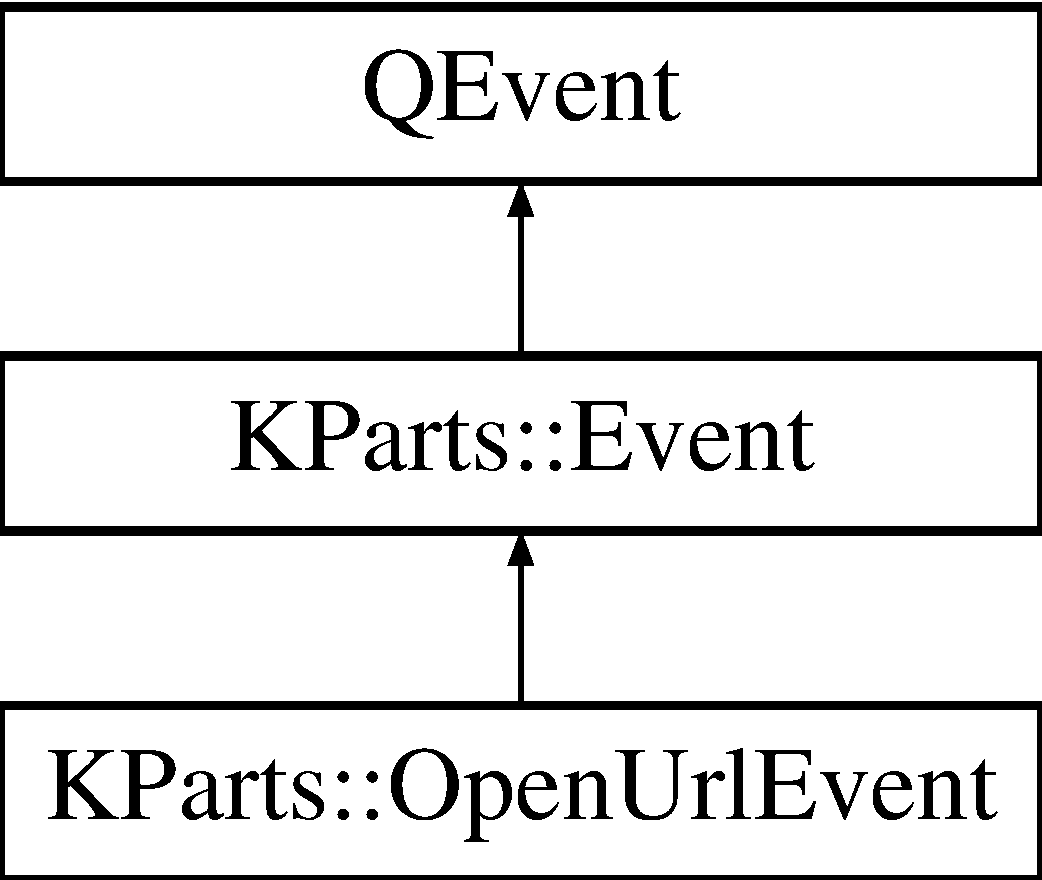
\includegraphics[height=2.000000cm]{classKParts_1_1OpenUrlEvent}
\end{center}
\end{figure}
\subsection*{\-Public \-Member \-Functions}
\begin{DoxyCompactItemize}
\item 
\hyperlink{classKParts_1_1OpenUrlEvent_af98b6f595f6aa62dca8d72ff54138ec9}{\-Open\-Url\-Event} (\hyperlink{classKParts_1_1ReadOnlyPart}{\-Read\-Only\-Part} $\ast$\hyperlink{classKParts_1_1OpenUrlEvent_a2c23bcde7fee2966c25dbd7d961b151b}{part}, const \-K\-Url \&\hyperlink{classKParts_1_1OpenUrlEvent_a910c8c089b7c863e49cd83ddf4b8f003}{url}, const \hyperlink{classKParts_1_1OpenUrlArguments}{\-Open\-Url\-Arguments} \&args=\hyperlink{classKParts_1_1OpenUrlArguments}{\-Open\-Url\-Arguments}(), const \hyperlink{structKParts_1_1BrowserArguments}{\-Browser\-Arguments} \&browser\-Args=\hyperlink{structKParts_1_1BrowserArguments}{\-Browser\-Arguments}())
\item 
virtual \hyperlink{classKParts_1_1OpenUrlEvent_aceb6c7fd12ae21889f779d7a074e02ca}{$\sim$\-Open\-Url\-Event} ()
\item 
\hyperlink{classKParts_1_1ReadOnlyPart}{\-Read\-Only\-Part} $\ast$ \hyperlink{classKParts_1_1OpenUrlEvent_a2c23bcde7fee2966c25dbd7d961b151b}{part} () const 
\item 
\-K\-Url \hyperlink{classKParts_1_1OpenUrlEvent_a910c8c089b7c863e49cd83ddf4b8f003}{url} () const 
\item 
\hyperlink{classKParts_1_1OpenUrlArguments}{\-Open\-Url\-Arguments} \hyperlink{classKParts_1_1OpenUrlEvent_a8a365e2cb9c4be571aa5c0c383280fa0}{arguments} () const 
\item 
\hyperlink{structKParts_1_1BrowserArguments}{\-Browser\-Arguments} \hyperlink{classKParts_1_1OpenUrlEvent_a410497aaab6fbe7c2ff0ab9ca86f32ab}{browser\-Arguments} () const 
\end{DoxyCompactItemize}
\subsection*{\-Static \-Public \-Member \-Functions}
\begin{DoxyCompactItemize}
\item 
static bool \hyperlink{classKParts_1_1OpenUrlEvent_aa2c34fa11ddbcbf9828661fe681bcb62}{test} (const \-Q\-Event $\ast$event)
\end{DoxyCompactItemize}


\subsection{\-Detailed \-Description}
\-The \hyperlink{classKParts_1_1OpenUrlEvent}{\-K\-Parts\-::\-Open\-Url\-Event} event informs that a given part has opened a given \-U\-R\-L. \-Applications can use this event to send this information to interested plugins.

\-The event should be sent before opening the \-U\-R\-L in the part, so that the plugins can use \hyperlink{classKParts_1_1OpenUrlEvent_a2c23bcde7fee2966c25dbd7d961b151b}{part()}-\/$>$\hyperlink{classKParts_1_1OpenUrlEvent_a910c8c089b7c863e49cd83ddf4b8f003}{url()} to get the old \-U\-R\-L. 

\-Definition at line 249 of file browserextension.\-h.



\subsection{\-Constructor \& \-Destructor \-Documentation}
\hypertarget{classKParts_1_1OpenUrlEvent_af98b6f595f6aa62dca8d72ff54138ec9}{\index{\-K\-Parts\-::\-Open\-Url\-Event@{\-K\-Parts\-::\-Open\-Url\-Event}!\-Open\-Url\-Event@{\-Open\-Url\-Event}}
\index{\-Open\-Url\-Event@{\-Open\-Url\-Event}!KParts::OpenUrlEvent@{\-K\-Parts\-::\-Open\-Url\-Event}}
\subsubsection[{\-Open\-Url\-Event}]{\setlength{\rightskip}{0pt plus 5cm}{\bf \-K\-Parts\-::\-Open\-Url\-Event\-::\-Open\-Url\-Event} (
\begin{DoxyParamCaption}
\item[{{\bf \-Read\-Only\-Part} $\ast$}]{part, }
\item[{const \-K\-Url \&}]{url, }
\item[{const {\bf \-Open\-Url\-Arguments} \&}]{args = {\ttfamily {\bf \-Open\-Url\-Arguments}()}, }
\item[{const {\bf \-Browser\-Arguments} \&}]{browser\-Args = {\ttfamily {\bf \-Browser\-Arguments}()}}
\end{DoxyParamCaption}
)}}\label{classKParts_1_1OpenUrlEvent_af98b6f595f6aa62dca8d72ff54138ec9}
\hypertarget{classKParts_1_1OpenUrlEvent_aceb6c7fd12ae21889f779d7a074e02ca}{\index{\-K\-Parts\-::\-Open\-Url\-Event@{\-K\-Parts\-::\-Open\-Url\-Event}!$\sim$\-Open\-Url\-Event@{$\sim$\-Open\-Url\-Event}}
\index{$\sim$\-Open\-Url\-Event@{$\sim$\-Open\-Url\-Event}!KParts::OpenUrlEvent@{\-K\-Parts\-::\-Open\-Url\-Event}}
\subsubsection[{$\sim$\-Open\-Url\-Event}]{\setlength{\rightskip}{0pt plus 5cm}virtual {\bf \-K\-Parts\-::\-Open\-Url\-Event\-::$\sim$\-Open\-Url\-Event} (
\begin{DoxyParamCaption}
{}
\end{DoxyParamCaption}
)\hspace{0.3cm}{\ttfamily  \mbox{[}virtual\mbox{]}}}}\label{classKParts_1_1OpenUrlEvent_aceb6c7fd12ae21889f779d7a074e02ca}


\subsection{\-Member \-Function \-Documentation}
\hypertarget{classKParts_1_1OpenUrlEvent_a8a365e2cb9c4be571aa5c0c383280fa0}{\index{\-K\-Parts\-::\-Open\-Url\-Event@{\-K\-Parts\-::\-Open\-Url\-Event}!arguments@{arguments}}
\index{arguments@{arguments}!KParts::OpenUrlEvent@{\-K\-Parts\-::\-Open\-Url\-Event}}
\subsubsection[{arguments}]{\setlength{\rightskip}{0pt plus 5cm}{\bf \-Open\-Url\-Arguments} {\bf \-K\-Parts\-::\-Open\-Url\-Event\-::arguments} (
\begin{DoxyParamCaption}
{}
\end{DoxyParamCaption}
) const}}\label{classKParts_1_1OpenUrlEvent_a8a365e2cb9c4be571aa5c0c383280fa0}
\hypertarget{classKParts_1_1OpenUrlEvent_a410497aaab6fbe7c2ff0ab9ca86f32ab}{\index{\-K\-Parts\-::\-Open\-Url\-Event@{\-K\-Parts\-::\-Open\-Url\-Event}!browser\-Arguments@{browser\-Arguments}}
\index{browser\-Arguments@{browser\-Arguments}!KParts::OpenUrlEvent@{\-K\-Parts\-::\-Open\-Url\-Event}}
\subsubsection[{browser\-Arguments}]{\setlength{\rightskip}{0pt plus 5cm}{\bf \-Browser\-Arguments} {\bf \-K\-Parts\-::\-Open\-Url\-Event\-::browser\-Arguments} (
\begin{DoxyParamCaption}
{}
\end{DoxyParamCaption}
) const}}\label{classKParts_1_1OpenUrlEvent_a410497aaab6fbe7c2ff0ab9ca86f32ab}
\hypertarget{classKParts_1_1OpenUrlEvent_a2c23bcde7fee2966c25dbd7d961b151b}{\index{\-K\-Parts\-::\-Open\-Url\-Event@{\-K\-Parts\-::\-Open\-Url\-Event}!part@{part}}
\index{part@{part}!KParts::OpenUrlEvent@{\-K\-Parts\-::\-Open\-Url\-Event}}
\subsubsection[{part}]{\setlength{\rightskip}{0pt plus 5cm}{\bf \-Read\-Only\-Part}$\ast$ {\bf \-K\-Parts\-::\-Open\-Url\-Event\-::part} (
\begin{DoxyParamCaption}
{}
\end{DoxyParamCaption}
) const}}\label{classKParts_1_1OpenUrlEvent_a2c23bcde7fee2966c25dbd7d961b151b}
\hypertarget{classKParts_1_1OpenUrlEvent_aa2c34fa11ddbcbf9828661fe681bcb62}{\index{\-K\-Parts\-::\-Open\-Url\-Event@{\-K\-Parts\-::\-Open\-Url\-Event}!test@{test}}
\index{test@{test}!KParts::OpenUrlEvent@{\-K\-Parts\-::\-Open\-Url\-Event}}
\subsubsection[{test}]{\setlength{\rightskip}{0pt plus 5cm}static bool {\bf \-K\-Parts\-::\-Open\-Url\-Event\-::test} (
\begin{DoxyParamCaption}
\item[{const \-Q\-Event $\ast$}]{event}
\end{DoxyParamCaption}
)\hspace{0.3cm}{\ttfamily  \mbox{[}static\mbox{]}}}}\label{classKParts_1_1OpenUrlEvent_aa2c34fa11ddbcbf9828661fe681bcb62}


\-Reimplemented from \hyperlink{classKParts_1_1Event_a825b18534ae37dae24f2a2b326db0629}{\-K\-Parts\-::\-Event}.

\hypertarget{classKParts_1_1OpenUrlEvent_a910c8c089b7c863e49cd83ddf4b8f003}{\index{\-K\-Parts\-::\-Open\-Url\-Event@{\-K\-Parts\-::\-Open\-Url\-Event}!url@{url}}
\index{url@{url}!KParts::OpenUrlEvent@{\-K\-Parts\-::\-Open\-Url\-Event}}
\subsubsection[{url}]{\setlength{\rightskip}{0pt plus 5cm}\-K\-Url {\bf \-K\-Parts\-::\-Open\-Url\-Event\-::url} (
\begin{DoxyParamCaption}
{}
\end{DoxyParamCaption}
) const}}\label{classKParts_1_1OpenUrlEvent_a910c8c089b7c863e49cd83ddf4b8f003}


\-The documentation for this class was generated from the following file\-:\begin{DoxyCompactItemize}
\item 
/usr/include/kparts/\hyperlink{browserextension_8h}{browserextension.\-h}\end{DoxyCompactItemize}

\hypertarget{classKParts_1_1Part}{\section{K\+Parts\+:\+:Part Class Reference}
\label{classKParts_1_1Part}\index{K\+Parts\+::\+Part@{K\+Parts\+::\+Part}}
}


{\ttfamily \#include $<$part.\+h$>$}

Inheritance diagram for K\+Parts\+:\+:Part\+:\begin{figure}[H]
\begin{center}
\leavevmode
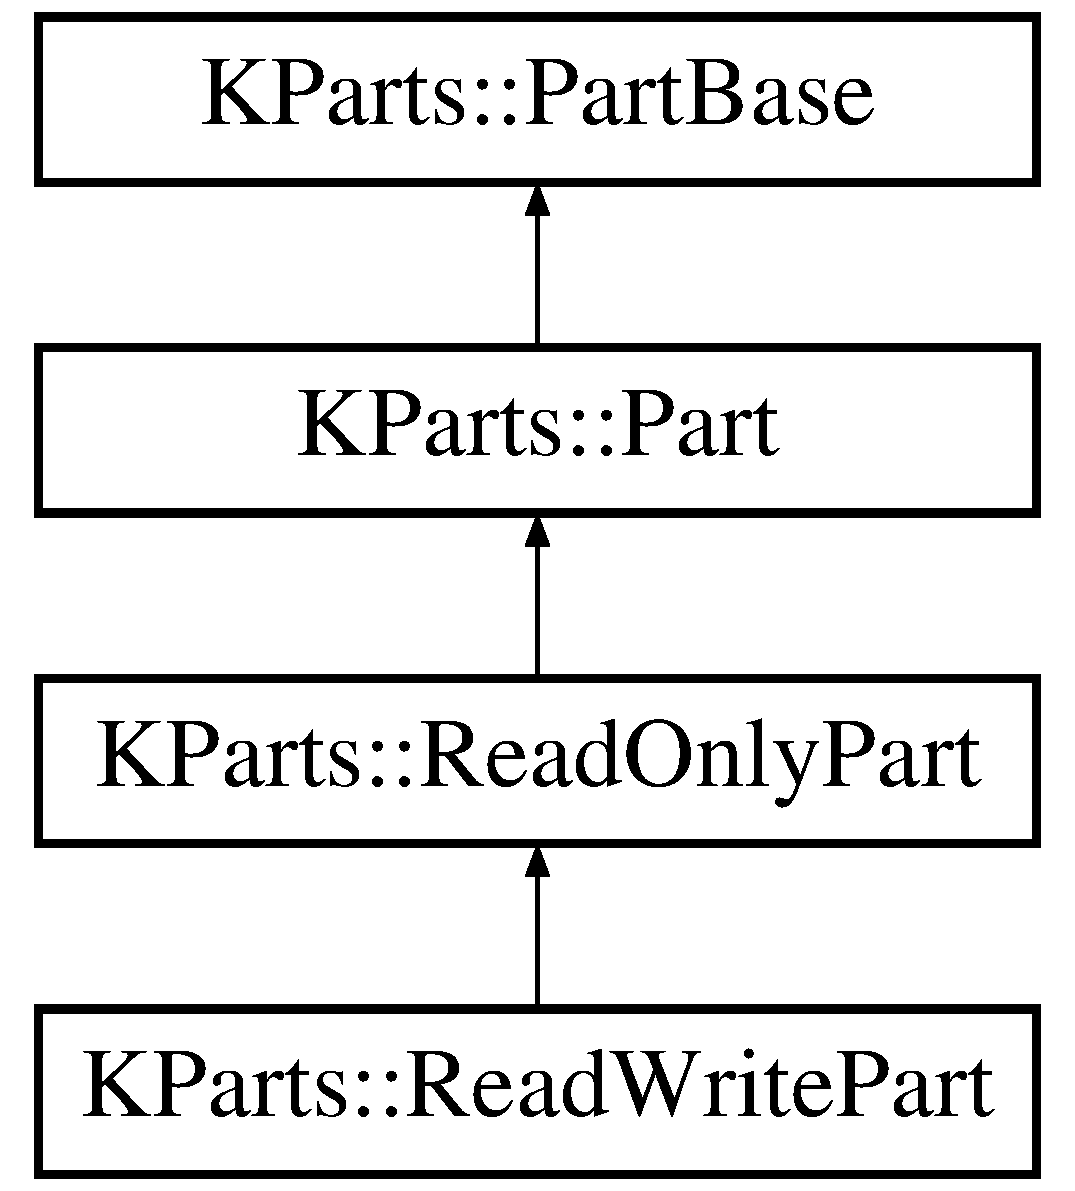
\includegraphics[height=7.000000cm]{classKParts_1_1Part}
\end{center}
\end{figure}
\subsection*{Signals}
\begin{DoxyCompactItemize}
\item 
void \hyperlink{classKParts_1_1Part_a00982292ef3d8b80dedeb5fed2376099}{set\+Window\+Caption} (const Q\+String \&caption)
\item 
void \hyperlink{classKParts_1_1Part_a809740a79edf0fa0bbe1dd982a6c4d35}{set\+Status\+Bar\+Text} (const Q\+String \&text)
\end{DoxyCompactItemize}
\subsection*{Public Member Functions}
\begin{DoxyCompactItemize}
\item 
\hyperlink{classKParts_1_1Part_afa61f98b2c9b14cbf94f9b1e2b453597}{Part} (Q\+Object $\ast$parent=0)
\item 
virtual \hyperlink{classKParts_1_1Part_a339e7a12833cdd5d4820d69070ea458b}{$\sim$\+Part} ()
\item 
virtual void \hyperlink{classKParts_1_1Part_afb9d58b0de422a96a809abade83c3922}{embed} (Q\+Widget $\ast$parent\+Widget)
\item 
virtual Q\+Widget $\ast$ \hyperlink{classKParts_1_1Part_a134900cb0605a1cd5113d90954a01fdf}{widget} ()
\item 
virtual void \hyperlink{classKParts_1_1Part_afb87e3aed12cfdd6ecf057f916c7889f}{set\+Manager} (\hyperlink{classKParts_1_1PartManager}{Part\+Manager} $\ast$\hyperlink{classKParts_1_1Part_a06ea4dd249752f23229bc30b693eed44}{manager})
\item 
\hyperlink{classKParts_1_1PartManager}{Part\+Manager} $\ast$ \hyperlink{classKParts_1_1Part_a06ea4dd249752f23229bc30b693eed44}{manager} () const 
\item 
void \hyperlink{classKParts_1_1Part_a18a6e6b02d7d08a52314d5a7a2d0a3bd}{set\+Auto\+Delete\+Widget} (bool auto\+Delete\+Widget)
\item 
void \hyperlink{classKParts_1_1Part_a0af0172fc3b5c585524ca5e84af05017}{set\+Auto\+Delete\+Part} (bool auto\+Delete\+Part)
\item 
virtual \hyperlink{classKParts_1_1Part}{Part} $\ast$ \hyperlink{classKParts_1_1Part_a5398eb6687f7136e2c02ec7f6f5fd66e}{hit\+Test} (Q\+Widget $\ast$\hyperlink{classKParts_1_1Part_a134900cb0605a1cd5113d90954a01fdf}{widget}, const Q\+Point \&global\+Pos)
\item 
virtual void \hyperlink{classKParts_1_1Part_aa4841b2e2ddb43de60e28ede88151f33}{set\+Selectable} (bool selectable)
\item 
bool \hyperlink{classKParts_1_1Part_a6c3e8845a5836a790ab67cb360120cab}{is\+Selectable} () const 
\item 
K\+Icon\+Loader $\ast$ \hyperlink{classKParts_1_1Part_a8c41d16009e44a35ec3b7c5e6b4e0b80}{icon\+Loader} ()
\end{DoxyCompactItemize}
\subsection*{Protected Slots}
\begin{DoxyCompactItemize}
\item 
void \hyperlink{classKParts_1_1Part_a07231742bae75d6fc5712aaf45397b29}{slot\+Widget\+Destroyed} ()
\end{DoxyCompactItemize}
\subsection*{Protected Member Functions}
\begin{DoxyCompactItemize}
\item 
virtual void \hyperlink{classKParts_1_1Part_a7578836b79ed97019b42f2d2fc03082d}{set\+Widget} (Q\+Widget $\ast$\hyperlink{classKParts_1_1Part_a134900cb0605a1cd5113d90954a01fdf}{widget})
\item 
virtual void \hyperlink{classKParts_1_1Part_a06a8a01b69df2ab366c5c5453b9194bd}{custom\+Event} (Q\+Event $\ast$event)
\item 
virtual void \hyperlink{classKParts_1_1Part_ad848641dbb38a3b2404b2ad554a08fba}{part\+Activate\+Event} (\hyperlink{classKParts_1_1PartActivateEvent}{Part\+Activate\+Event} $\ast$event)
\item 
virtual void \hyperlink{classKParts_1_1Part_a71a55af4b780e14d9ccadddfe7868941}{part\+Select\+Event} (\hyperlink{classKParts_1_1PartSelectEvent}{Part\+Select\+Event} $\ast$event)
\item 
virtual void \hyperlink{classKParts_1_1Part_a34b92f00459085ca7e05b7e8ee321347}{gui\+Activate\+Event} (\hyperlink{classKParts_1_1GUIActivateEvent}{G\+U\+I\+Activate\+Event} $\ast$event)
\item 
Q\+Widget $\ast$ \hyperlink{classKParts_1_1Part_a42ca0149d66ab5f2eea3d22b96300af0}{host\+Container} (const Q\+String \&container\+Name)
\item 
void \hyperlink{classKParts_1_1Part_aff25cf37e0d4e205028d75dee120828c}{load\+Plugins} ()
\item 
\hyperlink{classKParts_1_1Part_aa6c6292dcf062b5f4d711e6ab90070c9}{Part} (Part\+Private \&dd, Q\+Object $\ast$parent)
\end{DoxyCompactItemize}
\subsection*{Additional Inherited Members}


\subsection{Detailed Description}
Base class for parts.

A \char`\"{}part\char`\"{} is a G\+U\+I component, featuring\+: \begin{DoxyItemize}
\item A widget embeddedable in any application. \item G\+U\+I elements that will be merged in the \char`\"{}host\char`\"{} user interface (menubars, toolbars... ).\end{DoxyItemize}
{\bfseries About the widget\+:}\par
 Note that \hyperlink{classKParts_1_1Part}{K\+Parts\+::\+Part} does not inherit Q\+Widget. This is due to the fact that the \char`\"{}visual representation\char`\"{} will probably not be a mere Q\+Widget, but an elaborate one. That's why when implementing your \hyperlink{classKParts_1_1Part}{K\+Parts\+::\+Part} (or derived) you should call \hyperlink{classKParts_1_1Part_a7578836b79ed97019b42f2d2fc03082d}{K\+Parts\+::\+Part\+::set\+Widget()} in your constructor.

{\bfseries About the G\+U\+I elements\+:}\par
 Those elements trigger actions, defined by the part ( action()). The layout of the actions in the G\+U\+I is defined by an X\+M\+L file ( set\+X\+M\+L\+File()).

See also \hyperlink{classKParts_1_1ReadOnlyPart}{Read\+Only\+Part} and \hyperlink{classKParts_1_1ReadWritePart}{Read\+Write\+Part}, which define the framework for a \char`\"{}viewer\char`\"{} part and for an \char`\"{}editor\char`\"{}-\/like part. Use \hyperlink{classKParts_1_1Part}{Part} directly only if your part doesn't fit into those. 

Definition at line 215 of file part.\+h.



\subsection{Constructor \& Destructor Documentation}
\hypertarget{classKParts_1_1Part_afa61f98b2c9b14cbf94f9b1e2b453597}{\index{K\+Parts\+::\+Part@{K\+Parts\+::\+Part}!Part@{Part}}
\index{Part@{Part}!K\+Parts\+::\+Part@{K\+Parts\+::\+Part}}
\subsubsection[{Part}]{\setlength{\rightskip}{0pt plus 5cm}K\+Parts\+::\+Part\+::\+Part (
\begin{DoxyParamCaption}
\item[{Q\+Object $\ast$}]{parent = {\ttfamily 0}}
\end{DoxyParamCaption}
)\hspace{0.3cm}{\ttfamily [explicit]}}}\label{classKParts_1_1Part_afa61f98b2c9b14cbf94f9b1e2b453597}
Constructor.


\begin{DoxyParams}{Parameters}
{\em parent} & Parent object of the part. \\
\hline
\end{DoxyParams}
\hypertarget{classKParts_1_1Part_a339e7a12833cdd5d4820d69070ea458b}{\index{K\+Parts\+::\+Part@{K\+Parts\+::\+Part}!````~Part@{$\sim$\+Part}}
\index{````~Part@{$\sim$\+Part}!K\+Parts\+::\+Part@{K\+Parts\+::\+Part}}
\subsubsection[{$\sim$\+Part}]{\setlength{\rightskip}{0pt plus 5cm}virtual K\+Parts\+::\+Part\+::$\sim$\+Part (
\begin{DoxyParamCaption}
{}
\end{DoxyParamCaption}
)\hspace{0.3cm}{\ttfamily [virtual]}}}\label{classKParts_1_1Part_a339e7a12833cdd5d4820d69070ea458b}
Destructor. 

Reimplemented in \hyperlink{classOkular_1_1Part_ad9e36566a956f331bbc7c59a43613481}{Okular\+::\+Part}.

\hypertarget{classKParts_1_1Part_aa6c6292dcf062b5f4d711e6ab90070c9}{\index{K\+Parts\+::\+Part@{K\+Parts\+::\+Part}!Part@{Part}}
\index{Part@{Part}!K\+Parts\+::\+Part@{K\+Parts\+::\+Part}}
\subsubsection[{Part}]{\setlength{\rightskip}{0pt plus 5cm}K\+Parts\+::\+Part\+::\+Part (
\begin{DoxyParamCaption}
\item[{Part\+Private \&}]{dd, }
\item[{Q\+Object $\ast$}]{parent}
\end{DoxyParamCaption}
)\hspace{0.3cm}{\ttfamily [protected]}}}\label{classKParts_1_1Part_aa6c6292dcf062b5f4d711e6ab90070c9}


\subsection{Member Function Documentation}
\hypertarget{classKParts_1_1Part_a06a8a01b69df2ab366c5c5453b9194bd}{\index{K\+Parts\+::\+Part@{K\+Parts\+::\+Part}!custom\+Event@{custom\+Event}}
\index{custom\+Event@{custom\+Event}!K\+Parts\+::\+Part@{K\+Parts\+::\+Part}}
\subsubsection[{custom\+Event}]{\setlength{\rightskip}{0pt plus 5cm}virtual void K\+Parts\+::\+Part\+::custom\+Event (
\begin{DoxyParamCaption}
\item[{Q\+Event $\ast$}]{event}
\end{DoxyParamCaption}
)\hspace{0.3cm}{\ttfamily [protected]}, {\ttfamily [virtual]}}}\label{classKParts_1_1Part_a06a8a01b69df2ab366c5c5453b9194bd}
\hypertarget{classKParts_1_1Part_afb9d58b0de422a96a809abade83c3922}{\index{K\+Parts\+::\+Part@{K\+Parts\+::\+Part}!embed@{embed}}
\index{embed@{embed}!K\+Parts\+::\+Part@{K\+Parts\+::\+Part}}
\subsubsection[{embed}]{\setlength{\rightskip}{0pt plus 5cm}virtual void K\+Parts\+::\+Part\+::embed (
\begin{DoxyParamCaption}
\item[{Q\+Widget $\ast$}]{parent\+Widget}
\end{DoxyParamCaption}
)\hspace{0.3cm}{\ttfamily [virtual]}}}\label{classKParts_1_1Part_afb9d58b0de422a96a809abade83c3922}
Embed this part into a host widget.

You don't need to do this if you created the widget with the correct parent widget -\/ this is just a Q\+Widget\+::reparent(). Note that the \hyperlink{classKParts_1_1Part}{Part} is still the holder of the Q\+Widget, meaning that if you delete the \hyperlink{classKParts_1_1Part}{Part}, then the widget gets destroyed as well, and vice-\/versa. This method is not recommended since creating the widget with the correct parent is simpler anyway. \hypertarget{classKParts_1_1Part_a34b92f00459085ca7e05b7e8ee321347}{\index{K\+Parts\+::\+Part@{K\+Parts\+::\+Part}!gui\+Activate\+Event@{gui\+Activate\+Event}}
\index{gui\+Activate\+Event@{gui\+Activate\+Event}!K\+Parts\+::\+Part@{K\+Parts\+::\+Part}}
\subsubsection[{gui\+Activate\+Event}]{\setlength{\rightskip}{0pt plus 5cm}virtual void K\+Parts\+::\+Part\+::gui\+Activate\+Event (
\begin{DoxyParamCaption}
\item[{{\bf G\+U\+I\+Activate\+Event} $\ast$}]{event}
\end{DoxyParamCaption}
)\hspace{0.3cm}{\ttfamily [protected]}, {\ttfamily [virtual]}}}\label{classKParts_1_1Part_a34b92f00459085ca7e05b7e8ee321347}
Convenience method which is called when the \hyperlink{classKParts_1_1Part}{Part} received a \hyperlink{classKParts_1_1GUIActivateEvent}{G\+U\+I\+Activate\+Event} . Reimplement this if you don't want to reimplement event and test for the event yourself or even install an event filter. 

Reimplemented in \hyperlink{classKParts_1_1ReadOnlyPart_aa5ac9f161aef38a92bbf25891746cac0}{K\+Parts\+::\+Read\+Only\+Part}, and \hyperlink{classOkular_1_1Part_a71ea7975f3f712fff8f91ce47a80149c}{Okular\+::\+Part}.

\hypertarget{classKParts_1_1Part_a5398eb6687f7136e2c02ec7f6f5fd66e}{\index{K\+Parts\+::\+Part@{K\+Parts\+::\+Part}!hit\+Test@{hit\+Test}}
\index{hit\+Test@{hit\+Test}!K\+Parts\+::\+Part@{K\+Parts\+::\+Part}}
\subsubsection[{hit\+Test}]{\setlength{\rightskip}{0pt plus 5cm}virtual {\bf Part}$\ast$ K\+Parts\+::\+Part\+::hit\+Test (
\begin{DoxyParamCaption}
\item[{Q\+Widget $\ast$}]{widget, }
\item[{const Q\+Point \&}]{global\+Pos}
\end{DoxyParamCaption}
)\hspace{0.3cm}{\ttfamily [virtual]}}}\label{classKParts_1_1Part_a5398eb6687f7136e2c02ec7f6f5fd66e}
Returns the part (this, or a child part) at the given global position. This is called by the part manager to ask whether a part should be activated when clicking somewhere. In most cases the default implementation is enough. Reimplement this if your part has child parts in some areas (like in khtml or koffice) 
\begin{DoxyParams}{Parameters}
{\em widget} & the part widget being clicked -\/ usually the same as \hyperlink{classKParts_1_1Part_a134900cb0605a1cd5113d90954a01fdf}{widget()}, except in koffice. \\
\hline
{\em global\+Pos} & the mouse coordinates in global coordinates \\
\hline
\end{DoxyParams}
\hypertarget{classKParts_1_1Part_a42ca0149d66ab5f2eea3d22b96300af0}{\index{K\+Parts\+::\+Part@{K\+Parts\+::\+Part}!host\+Container@{host\+Container}}
\index{host\+Container@{host\+Container}!K\+Parts\+::\+Part@{K\+Parts\+::\+Part}}
\subsubsection[{host\+Container}]{\setlength{\rightskip}{0pt plus 5cm}Q\+Widget$\ast$ K\+Parts\+::\+Part\+::host\+Container (
\begin{DoxyParamCaption}
\item[{const Q\+String \&}]{container\+Name}
\end{DoxyParamCaption}
)\hspace{0.3cm}{\ttfamily [protected]}}}\label{classKParts_1_1Part_a42ca0149d66ab5f2eea3d22b96300af0}
Convenience method for K\+X\+M\+L\+G\+U\+I\+Factory\+::container. \begin{DoxyReturn}{Returns}
a container widget owned by the \hyperlink{classKParts_1_1Part}{Part}'s G\+U\+I. 
\end{DoxyReturn}
\hypertarget{classKParts_1_1Part_a8c41d16009e44a35ec3b7c5e6b4e0b80}{\index{K\+Parts\+::\+Part@{K\+Parts\+::\+Part}!icon\+Loader@{icon\+Loader}}
\index{icon\+Loader@{icon\+Loader}!K\+Parts\+::\+Part@{K\+Parts\+::\+Part}}
\subsubsection[{icon\+Loader}]{\setlength{\rightskip}{0pt plus 5cm}K\+Icon\+Loader$\ast$ K\+Parts\+::\+Part\+::icon\+Loader (
\begin{DoxyParamCaption}
{}
\end{DoxyParamCaption}
)}}\label{classKParts_1_1Part_a8c41d16009e44a35ec3b7c5e6b4e0b80}
Use this icon loader to load any icons that are specific to this part, i.\+e. icons installed into this part's own directories as opposed to standard kde icons. Use K\+Icon(\char`\"{}myicon\char`\"{}, \hyperlink{classKParts_1_1Part_a8c41d16009e44a35ec3b7c5e6b4e0b80}{icon\+Loader()}).

Make sure to call set\+Component\+Data before calling icon\+Loader. \hypertarget{classKParts_1_1Part_a6c3e8845a5836a790ab67cb360120cab}{\index{K\+Parts\+::\+Part@{K\+Parts\+::\+Part}!is\+Selectable@{is\+Selectable}}
\index{is\+Selectable@{is\+Selectable}!K\+Parts\+::\+Part@{K\+Parts\+::\+Part}}
\subsubsection[{is\+Selectable}]{\setlength{\rightskip}{0pt plus 5cm}bool K\+Parts\+::\+Part\+::is\+Selectable (
\begin{DoxyParamCaption}
{}
\end{DoxyParamCaption}
) const}}\label{classKParts_1_1Part_a6c3e8845a5836a790ab67cb360120cab}
Returns whether the part is selectable or not. \hypertarget{classKParts_1_1Part_aff25cf37e0d4e205028d75dee120828c}{\index{K\+Parts\+::\+Part@{K\+Parts\+::\+Part}!load\+Plugins@{load\+Plugins}}
\index{load\+Plugins@{load\+Plugins}!K\+Parts\+::\+Part@{K\+Parts\+::\+Part}}
\subsubsection[{load\+Plugins}]{\setlength{\rightskip}{0pt plus 5cm}void K\+Parts\+::\+Part\+::load\+Plugins (
\begin{DoxyParamCaption}
{}
\end{DoxyParamCaption}
)\hspace{0.3cm}{\ttfamily [protected]}}}\label{classKParts_1_1Part_aff25cf37e0d4e205028d75dee120828c}
Load this part's plugins now. Normally you want to call this at the end of the part constructor, if you used set\+Component\+Data(component\+Data, false) \begin{DoxySince}{Since}
4.\+1 
\end{DoxySince}
\hypertarget{classKParts_1_1Part_a06ea4dd249752f23229bc30b693eed44}{\index{K\+Parts\+::\+Part@{K\+Parts\+::\+Part}!manager@{manager}}
\index{manager@{manager}!K\+Parts\+::\+Part@{K\+Parts\+::\+Part}}
\subsubsection[{manager}]{\setlength{\rightskip}{0pt plus 5cm}{\bf Part\+Manager}$\ast$ K\+Parts\+::\+Part\+::manager (
\begin{DoxyParamCaption}
{}
\end{DoxyParamCaption}
) const}}\label{classKParts_1_1Part_a06ea4dd249752f23229bc30b693eed44}
Returns the part manager handling this part, if any (0\+L otherwise). \hypertarget{classKParts_1_1Part_ad848641dbb38a3b2404b2ad554a08fba}{\index{K\+Parts\+::\+Part@{K\+Parts\+::\+Part}!part\+Activate\+Event@{part\+Activate\+Event}}
\index{part\+Activate\+Event@{part\+Activate\+Event}!K\+Parts\+::\+Part@{K\+Parts\+::\+Part}}
\subsubsection[{part\+Activate\+Event}]{\setlength{\rightskip}{0pt plus 5cm}virtual void K\+Parts\+::\+Part\+::part\+Activate\+Event (
\begin{DoxyParamCaption}
\item[{{\bf Part\+Activate\+Event} $\ast$}]{event}
\end{DoxyParamCaption}
)\hspace{0.3cm}{\ttfamily [protected]}, {\ttfamily [virtual]}}}\label{classKParts_1_1Part_ad848641dbb38a3b2404b2ad554a08fba}
Convenience method which is called when the \hyperlink{classKParts_1_1Part}{Part} received a \hyperlink{classKParts_1_1PartActivateEvent}{Part\+Activate\+Event} . Reimplement this if you don't want to reimplement event and test for the event yourself or even install an event filter. \hypertarget{classKParts_1_1Part_a71a55af4b780e14d9ccadddfe7868941}{\index{K\+Parts\+::\+Part@{K\+Parts\+::\+Part}!part\+Select\+Event@{part\+Select\+Event}}
\index{part\+Select\+Event@{part\+Select\+Event}!K\+Parts\+::\+Part@{K\+Parts\+::\+Part}}
\subsubsection[{part\+Select\+Event}]{\setlength{\rightskip}{0pt plus 5cm}virtual void K\+Parts\+::\+Part\+::part\+Select\+Event (
\begin{DoxyParamCaption}
\item[{{\bf Part\+Select\+Event} $\ast$}]{event}
\end{DoxyParamCaption}
)\hspace{0.3cm}{\ttfamily [protected]}, {\ttfamily [virtual]}}}\label{classKParts_1_1Part_a71a55af4b780e14d9ccadddfe7868941}
Convenience method which is called when the \hyperlink{classKParts_1_1Part}{Part} received a \hyperlink{classKParts_1_1PartSelectEvent}{Part\+Select\+Event} . Reimplement this if you don't want to reimplement event and test for the event yourself or even install an event filter. \hypertarget{classKParts_1_1Part_a0af0172fc3b5c585524ca5e84af05017}{\index{K\+Parts\+::\+Part@{K\+Parts\+::\+Part}!set\+Auto\+Delete\+Part@{set\+Auto\+Delete\+Part}}
\index{set\+Auto\+Delete\+Part@{set\+Auto\+Delete\+Part}!K\+Parts\+::\+Part@{K\+Parts\+::\+Part}}
\subsubsection[{set\+Auto\+Delete\+Part}]{\setlength{\rightskip}{0pt plus 5cm}void K\+Parts\+::\+Part\+::set\+Auto\+Delete\+Part (
\begin{DoxyParamCaption}
\item[{bool}]{auto\+Delete\+Part}
\end{DoxyParamCaption}
)}}\label{classKParts_1_1Part_a0af0172fc3b5c585524ca5e84af05017}
By default, the part deletes itself when its widget is deleted. The hosting application can call set\+Auto\+Delete\+Part(false) to disable this behavior, to be able to delete the widget and then the part, independently. This is a method for the hosting application only, \hyperlink{classKParts_1_1Part}{Part} subclasses should never call this. \hypertarget{classKParts_1_1Part_a18a6e6b02d7d08a52314d5a7a2d0a3bd}{\index{K\+Parts\+::\+Part@{K\+Parts\+::\+Part}!set\+Auto\+Delete\+Widget@{set\+Auto\+Delete\+Widget}}
\index{set\+Auto\+Delete\+Widget@{set\+Auto\+Delete\+Widget}!K\+Parts\+::\+Part@{K\+Parts\+::\+Part}}
\subsubsection[{set\+Auto\+Delete\+Widget}]{\setlength{\rightskip}{0pt plus 5cm}void K\+Parts\+::\+Part\+::set\+Auto\+Delete\+Widget (
\begin{DoxyParamCaption}
\item[{bool}]{auto\+Delete\+Widget}
\end{DoxyParamCaption}
)}}\label{classKParts_1_1Part_a18a6e6b02d7d08a52314d5a7a2d0a3bd}
By default, the widget is deleted by the part when the part is deleted. The hosting application can call set\+Auto\+Delete\+Widget(false) to disable this behavior, given that the widget is usually deleted by its parent widget anyway. This is a method for the hosting application only, \hyperlink{classKParts_1_1Part}{Part} subclasses should never call this. \hypertarget{classKParts_1_1Part_afb87e3aed12cfdd6ecf057f916c7889f}{\index{K\+Parts\+::\+Part@{K\+Parts\+::\+Part}!set\+Manager@{set\+Manager}}
\index{set\+Manager@{set\+Manager}!K\+Parts\+::\+Part@{K\+Parts\+::\+Part}}
\subsubsection[{set\+Manager}]{\setlength{\rightskip}{0pt plus 5cm}virtual void K\+Parts\+::\+Part\+::set\+Manager (
\begin{DoxyParamCaption}
\item[{{\bf Part\+Manager} $\ast$}]{manager}
\end{DoxyParamCaption}
)\hspace{0.3cm}{\ttfamily [virtual]}}}\label{classKParts_1_1Part_afb87e3aed12cfdd6ecf057f916c7889f}
\hypertarget{classKParts_1_1Part_aa4841b2e2ddb43de60e28ede88151f33}{\index{K\+Parts\+::\+Part@{K\+Parts\+::\+Part}!set\+Selectable@{set\+Selectable}}
\index{set\+Selectable@{set\+Selectable}!K\+Parts\+::\+Part@{K\+Parts\+::\+Part}}
\subsubsection[{set\+Selectable}]{\setlength{\rightskip}{0pt plus 5cm}virtual void K\+Parts\+::\+Part\+::set\+Selectable (
\begin{DoxyParamCaption}
\item[{bool}]{selectable}
\end{DoxyParamCaption}
)\hspace{0.3cm}{\ttfamily [virtual]}}}\label{classKParts_1_1Part_aa4841b2e2ddb43de60e28ede88151f33}

\begin{DoxyParams}{Parameters}
{\em selectable} & Indicates whether the part is selectable or not. \\
\hline
\end{DoxyParams}
\hypertarget{classKParts_1_1Part_a809740a79edf0fa0bbe1dd982a6c4d35}{\index{K\+Parts\+::\+Part@{K\+Parts\+::\+Part}!set\+Status\+Bar\+Text@{set\+Status\+Bar\+Text}}
\index{set\+Status\+Bar\+Text@{set\+Status\+Bar\+Text}!K\+Parts\+::\+Part@{K\+Parts\+::\+Part}}
\subsubsection[{set\+Status\+Bar\+Text}]{\setlength{\rightskip}{0pt plus 5cm}void K\+Parts\+::\+Part\+::set\+Status\+Bar\+Text (
\begin{DoxyParamCaption}
\item[{const Q\+String \&}]{text}
\end{DoxyParamCaption}
)\hspace{0.3cm}{\ttfamily [signal]}}}\label{classKParts_1_1Part_a809740a79edf0fa0bbe1dd982a6c4d35}
Emitted by the part, to set a text in the statusbar of the window(s) hosting this part \hypertarget{classKParts_1_1Part_a7578836b79ed97019b42f2d2fc03082d}{\index{K\+Parts\+::\+Part@{K\+Parts\+::\+Part}!set\+Widget@{set\+Widget}}
\index{set\+Widget@{set\+Widget}!K\+Parts\+::\+Part@{K\+Parts\+::\+Part}}
\subsubsection[{set\+Widget}]{\setlength{\rightskip}{0pt plus 5cm}virtual void K\+Parts\+::\+Part\+::set\+Widget (
\begin{DoxyParamCaption}
\item[{Q\+Widget $\ast$}]{widget}
\end{DoxyParamCaption}
)\hspace{0.3cm}{\ttfamily [protected]}, {\ttfamily [virtual]}}}\label{classKParts_1_1Part_a7578836b79ed97019b42f2d2fc03082d}
Set the main widget.

Call this in the Part-\/inherited class constructor. \hypertarget{classKParts_1_1Part_a00982292ef3d8b80dedeb5fed2376099}{\index{K\+Parts\+::\+Part@{K\+Parts\+::\+Part}!set\+Window\+Caption@{set\+Window\+Caption}}
\index{set\+Window\+Caption@{set\+Window\+Caption}!K\+Parts\+::\+Part@{K\+Parts\+::\+Part}}
\subsubsection[{set\+Window\+Caption}]{\setlength{\rightskip}{0pt plus 5cm}void K\+Parts\+::\+Part\+::set\+Window\+Caption (
\begin{DoxyParamCaption}
\item[{const Q\+String \&}]{caption}
\end{DoxyParamCaption}
)\hspace{0.3cm}{\ttfamily [signal]}}}\label{classKParts_1_1Part_a00982292ef3d8b80dedeb5fed2376099}
Emitted by the part, to set the caption of the window(s) hosting this part \hypertarget{classKParts_1_1Part_a07231742bae75d6fc5712aaf45397b29}{\index{K\+Parts\+::\+Part@{K\+Parts\+::\+Part}!slot\+Widget\+Destroyed@{slot\+Widget\+Destroyed}}
\index{slot\+Widget\+Destroyed@{slot\+Widget\+Destroyed}!K\+Parts\+::\+Part@{K\+Parts\+::\+Part}}
\subsubsection[{slot\+Widget\+Destroyed}]{\setlength{\rightskip}{0pt plus 5cm}void K\+Parts\+::\+Part\+::slot\+Widget\+Destroyed (
\begin{DoxyParamCaption}
{}
\end{DoxyParamCaption}
)\hspace{0.3cm}{\ttfamily [protected]}, {\ttfamily [slot]}}}\label{classKParts_1_1Part_a07231742bae75d6fc5712aaf45397b29}
\hypertarget{classKParts_1_1Part_a134900cb0605a1cd5113d90954a01fdf}{\index{K\+Parts\+::\+Part@{K\+Parts\+::\+Part}!widget@{widget}}
\index{widget@{widget}!K\+Parts\+::\+Part@{K\+Parts\+::\+Part}}
\subsubsection[{widget}]{\setlength{\rightskip}{0pt plus 5cm}virtual Q\+Widget$\ast$ K\+Parts\+::\+Part\+::widget (
\begin{DoxyParamCaption}
{}
\end{DoxyParamCaption}
)\hspace{0.3cm}{\ttfamily [virtual]}}}\label{classKParts_1_1Part_a134900cb0605a1cd5113d90954a01fdf}
\begin{DoxyReturn}{Returns}
The widget defined by this part, set by \hyperlink{classKParts_1_1Part_a7578836b79ed97019b42f2d2fc03082d}{set\+Widget()}. 
\end{DoxyReturn}


The documentation for this class was generated from the following file\+:\begin{DoxyCompactItemize}
\item 
/usr/include/kparts/\hyperlink{usr_2include_2kparts_2part_8h}{part.\+h}\end{DoxyCompactItemize}

\hypertarget{classKParts_1_1PartActivateEvent}{\section{K\+Parts\+:\+:Part\+Activate\+Event Class Reference}
\label{classKParts_1_1PartActivateEvent}\index{K\+Parts\+::\+Part\+Activate\+Event@{K\+Parts\+::\+Part\+Activate\+Event}}
}


{\ttfamily \#include $<$event.\+h$>$}

Inheritance diagram for K\+Parts\+:\+:Part\+Activate\+Event\+:\begin{figure}[H]
\begin{center}
\leavevmode
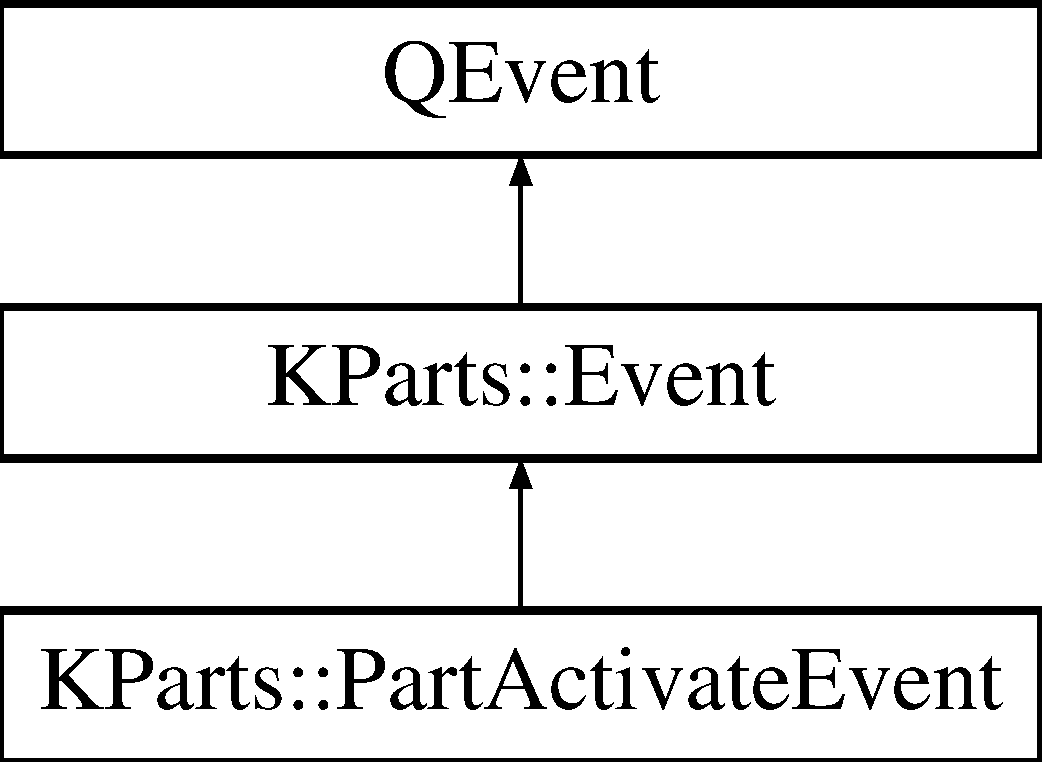
\includegraphics[height=3.000000cm]{classKParts_1_1PartActivateEvent}
\end{center}
\end{figure}
\subsection*{Public Member Functions}
\begin{DoxyCompactItemize}
\item 
\hyperlink{classKParts_1_1PartActivateEvent_a6b2b2b39fc6e8518b74e74f0f5f3947d}{Part\+Activate\+Event} (bool \hyperlink{classKParts_1_1PartActivateEvent_a7d6c164caa76842171eed19df734715b}{activated}, \hyperlink{classKParts_1_1Part}{Part} $\ast$\hyperlink{classKParts_1_1PartActivateEvent_a5588cf3b52a16cc65586a3faf6523117}{part}, Q\+Widget $\ast$\hyperlink{classKParts_1_1PartActivateEvent_ae3ec0f57c3c257eb13e4cf8c5d551f81}{widget})
\item 
virtual \hyperlink{classKParts_1_1PartActivateEvent_a070038fad91c9494c6ef4dfd00401f62}{$\sim$\+Part\+Activate\+Event} ()
\item 
bool \hyperlink{classKParts_1_1PartActivateEvent_a7d6c164caa76842171eed19df734715b}{activated} () const 
\item 
\hyperlink{classKParts_1_1Part}{Part} $\ast$ \hyperlink{classKParts_1_1PartActivateEvent_a5588cf3b52a16cc65586a3faf6523117}{part} () const 
\item 
Q\+Widget $\ast$ \hyperlink{classKParts_1_1PartActivateEvent_ae3ec0f57c3c257eb13e4cf8c5d551f81}{widget} () const 
\end{DoxyCompactItemize}
\subsection*{Static Public Member Functions}
\begin{DoxyCompactItemize}
\item 
static bool \hyperlink{classKParts_1_1PartActivateEvent_ab2b795f3ff5ed09524e0357ee21cf264}{test} (const Q\+Event $\ast$event)
\end{DoxyCompactItemize}


\subsection{Detailed Description}
This event is sent by the part manager when the active part changes. Each time the active part changes, it will send first a \hyperlink{classKParts_1_1PartActivateEvent}{Part\+Activate\+Event} with activated=false, part=old\+Active\+Part, widget=old\+Active\+Widget and then another \hyperlink{classKParts_1_1PartActivateEvent}{Part\+Activate\+Event} with activated=true, part=new\+Part, widget=new\+Widget. \begin{DoxySeeAlso}{See Also}
\hyperlink{classKParts_1_1Part_ad848641dbb38a3b2404b2ad554a08fba}{K\+Parts\+::\+Part\+::part\+Activate\+Event} 
\end{DoxySeeAlso}


Definition at line 82 of file event.\+h.



\subsection{Constructor \& Destructor Documentation}
\hypertarget{classKParts_1_1PartActivateEvent_a6b2b2b39fc6e8518b74e74f0f5f3947d}{\index{K\+Parts\+::\+Part\+Activate\+Event@{K\+Parts\+::\+Part\+Activate\+Event}!Part\+Activate\+Event@{Part\+Activate\+Event}}
\index{Part\+Activate\+Event@{Part\+Activate\+Event}!K\+Parts\+::\+Part\+Activate\+Event@{K\+Parts\+::\+Part\+Activate\+Event}}
\subsubsection[{Part\+Activate\+Event}]{\setlength{\rightskip}{0pt plus 5cm}K\+Parts\+::\+Part\+Activate\+Event\+::\+Part\+Activate\+Event (
\begin{DoxyParamCaption}
\item[{bool}]{activated, }
\item[{{\bf Part} $\ast$}]{part, }
\item[{Q\+Widget $\ast$}]{widget}
\end{DoxyParamCaption}
)}}\label{classKParts_1_1PartActivateEvent_a6b2b2b39fc6e8518b74e74f0f5f3947d}
\hypertarget{classKParts_1_1PartActivateEvent_a070038fad91c9494c6ef4dfd00401f62}{\index{K\+Parts\+::\+Part\+Activate\+Event@{K\+Parts\+::\+Part\+Activate\+Event}!````~Part\+Activate\+Event@{$\sim$\+Part\+Activate\+Event}}
\index{````~Part\+Activate\+Event@{$\sim$\+Part\+Activate\+Event}!K\+Parts\+::\+Part\+Activate\+Event@{K\+Parts\+::\+Part\+Activate\+Event}}
\subsubsection[{$\sim$\+Part\+Activate\+Event}]{\setlength{\rightskip}{0pt plus 5cm}virtual K\+Parts\+::\+Part\+Activate\+Event\+::$\sim$\+Part\+Activate\+Event (
\begin{DoxyParamCaption}
{}
\end{DoxyParamCaption}
)\hspace{0.3cm}{\ttfamily [virtual]}}}\label{classKParts_1_1PartActivateEvent_a070038fad91c9494c6ef4dfd00401f62}


\subsection{Member Function Documentation}
\hypertarget{classKParts_1_1PartActivateEvent_a7d6c164caa76842171eed19df734715b}{\index{K\+Parts\+::\+Part\+Activate\+Event@{K\+Parts\+::\+Part\+Activate\+Event}!activated@{activated}}
\index{activated@{activated}!K\+Parts\+::\+Part\+Activate\+Event@{K\+Parts\+::\+Part\+Activate\+Event}}
\subsubsection[{activated}]{\setlength{\rightskip}{0pt plus 5cm}bool K\+Parts\+::\+Part\+Activate\+Event\+::activated (
\begin{DoxyParamCaption}
{}
\end{DoxyParamCaption}
) const}}\label{classKParts_1_1PartActivateEvent_a7d6c164caa76842171eed19df734715b}
\hypertarget{classKParts_1_1PartActivateEvent_a5588cf3b52a16cc65586a3faf6523117}{\index{K\+Parts\+::\+Part\+Activate\+Event@{K\+Parts\+::\+Part\+Activate\+Event}!part@{part}}
\index{part@{part}!K\+Parts\+::\+Part\+Activate\+Event@{K\+Parts\+::\+Part\+Activate\+Event}}
\subsubsection[{part}]{\setlength{\rightskip}{0pt plus 5cm}{\bf Part}$\ast$ K\+Parts\+::\+Part\+Activate\+Event\+::part (
\begin{DoxyParamCaption}
{}
\end{DoxyParamCaption}
) const}}\label{classKParts_1_1PartActivateEvent_a5588cf3b52a16cc65586a3faf6523117}
\hypertarget{classKParts_1_1PartActivateEvent_ab2b795f3ff5ed09524e0357ee21cf264}{\index{K\+Parts\+::\+Part\+Activate\+Event@{K\+Parts\+::\+Part\+Activate\+Event}!test@{test}}
\index{test@{test}!K\+Parts\+::\+Part\+Activate\+Event@{K\+Parts\+::\+Part\+Activate\+Event}}
\subsubsection[{test}]{\setlength{\rightskip}{0pt plus 5cm}static bool K\+Parts\+::\+Part\+Activate\+Event\+::test (
\begin{DoxyParamCaption}
\item[{const Q\+Event $\ast$}]{event}
\end{DoxyParamCaption}
)\hspace{0.3cm}{\ttfamily [static]}}}\label{classKParts_1_1PartActivateEvent_ab2b795f3ff5ed09524e0357ee21cf264}
\hypertarget{classKParts_1_1PartActivateEvent_ae3ec0f57c3c257eb13e4cf8c5d551f81}{\index{K\+Parts\+::\+Part\+Activate\+Event@{K\+Parts\+::\+Part\+Activate\+Event}!widget@{widget}}
\index{widget@{widget}!K\+Parts\+::\+Part\+Activate\+Event@{K\+Parts\+::\+Part\+Activate\+Event}}
\subsubsection[{widget}]{\setlength{\rightskip}{0pt plus 5cm}Q\+Widget$\ast$ K\+Parts\+::\+Part\+Activate\+Event\+::widget (
\begin{DoxyParamCaption}
{}
\end{DoxyParamCaption}
) const}}\label{classKParts_1_1PartActivateEvent_ae3ec0f57c3c257eb13e4cf8c5d551f81}


The documentation for this class was generated from the following file\+:\begin{DoxyCompactItemize}
\item 
/usr/include/kparts/\hyperlink{event_8h}{event.\+h}\end{DoxyCompactItemize}

\hypertarget{classKParts_1_1PartBase}{\section{\-K\-Parts\-:\-:\-Part\-Base \-Class \-Reference}
\label{classKParts_1_1PartBase}\index{\-K\-Parts\-::\-Part\-Base@{\-K\-Parts\-::\-Part\-Base}}
}


\-Base class for all parts.  




{\ttfamily \#include $<$part.\-h$>$}

\-Inheritance diagram for \-K\-Parts\-:\-:\-Part\-Base\-:\begin{figure}[H]
\begin{center}
\leavevmode
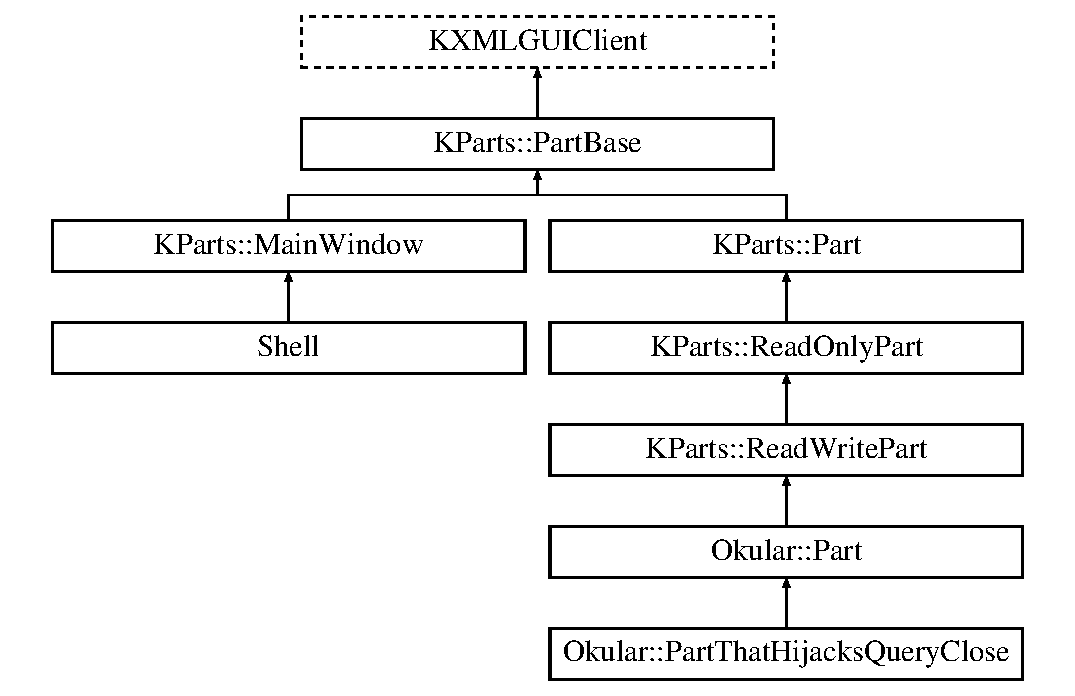
\includegraphics[height=4.000000cm]{classKParts_1_1PartBase}
\end{center}
\end{figure}
\subsection*{\-Public \-Member \-Functions}
\begin{DoxyCompactItemize}
\item 
\hyperlink{classKParts_1_1PartBase_a24a84cc28a2f2c351d39c4128f2952a0}{\-Part\-Base} ()
\item 
virtual \hyperlink{classKParts_1_1PartBase_a0753290f4dd3c2886425e37594939ea8}{$\sim$\-Part\-Base} ()
\item 
void \hyperlink{classKParts_1_1PartBase_aea74884035b19b8909c3163ad6afd444}{set\-Part\-Object} (\-Q\-Object $\ast$object)
\item 
\-Q\-Object $\ast$ \hyperlink{classKParts_1_1PartBase_a259f6a9c7258d1a623b56782391ac7e6}{part\-Object} () const 
\end{DoxyCompactItemize}
\subsection*{\-Protected \-Types}
\begin{DoxyCompactItemize}
\item 
enum \hyperlink{classKParts_1_1PartBase_a73b04eba759c3505ac722b2ceaaa8b76}{\-Plugin\-Loading\-Mode} \{ \hyperlink{classKParts_1_1PartBase_a73b04eba759c3505ac722b2ceaaa8b76a3ffe0a5005d5e1d00b4d3fd8c4d51a1e}{\-Do\-Not\-Load\-Plugins} =  0, 
\hyperlink{classKParts_1_1PartBase_a73b04eba759c3505ac722b2ceaaa8b76aeff505f5627f1539e03730d042e39522}{\-Load\-Plugins} =  1, 
\hyperlink{classKParts_1_1PartBase_a73b04eba759c3505ac722b2ceaaa8b76aeaf6ca999ef635e22e3f52234226e931}{\-Load\-Plugins\-If\-Enabled} =  2
 \}
\end{DoxyCompactItemize}
\subsection*{\-Protected \-Member \-Functions}
\begin{DoxyCompactItemize}
\item 
virtual void \hyperlink{classKParts_1_1PartBase_a5542df2a60d5ed1882bf31ac89d9a8fe}{set\-Component\-Data} (const \-K\-Component\-Data \&component\-Data)
\item 
virtual void \hyperlink{classKParts_1_1PartBase_af8ef8d076e01eda7b03fadca80b41afc}{set\-Component\-Data} (const \-K\-Component\-Data \&component\-Data, bool \hyperlink{classKParts_1_1PartBase_aca02ff148518a56d98a1fc8e96d7f637}{load\-Plugins})
\item 
void \hyperlink{classKParts_1_1PartBase_aca02ff148518a56d98a1fc8e96d7f637}{load\-Plugins} (\-Q\-Object $\ast$parent, \-K\-X\-M\-L\-G\-U\-I\-Client $\ast$parent\-G\-U\-I\-Client, const \-K\-Component\-Data \&component\-Data)
\item 
void \hyperlink{classKParts_1_1PartBase_abaf6f9e33fa1890008905f9a1356e1a1}{set\-Plugin\-Loading\-Mode} (\hyperlink{classKParts_1_1PartBase_a73b04eba759c3505ac722b2ceaaa8b76}{\-Plugin\-Loading\-Mode} loading\-Mode)
\item 
void \hyperlink{classKParts_1_1PartBase_a5a9ed59560edb848e787c4b3cee878b1}{set\-Plugin\-Interface\-Version} (int version)
\item 
\hyperlink{classKParts_1_1PartBase_acf7602b6a274df3a055ef39dcda3b6ed}{\-Part\-Base} (\-Part\-Base\-Private \&dd)
\end{DoxyCompactItemize}
\subsection*{\-Protected \-Attributes}
\begin{DoxyCompactItemize}
\item 
\-Part\-Base\-Private $\ast$ \hyperlink{classKParts_1_1PartBase_a5655e19a6338ea12c0e0a92956277e08}{d\-\_\-ptr}
\end{DoxyCompactItemize}


\subsection{\-Detailed \-Description}
\-Base class for all parts. 

\-Definition at line 64 of file part.\-h.



\subsection{\-Member \-Enumeration \-Documentation}
\hypertarget{classKParts_1_1PartBase_a73b04eba759c3505ac722b2ceaaa8b76}{\index{\-K\-Parts\-::\-Part\-Base@{\-K\-Parts\-::\-Part\-Base}!\-Plugin\-Loading\-Mode@{\-Plugin\-Loading\-Mode}}
\index{\-Plugin\-Loading\-Mode@{\-Plugin\-Loading\-Mode}!KParts::PartBase@{\-K\-Parts\-::\-Part\-Base}}
\subsubsection[{\-Plugin\-Loading\-Mode}]{\setlength{\rightskip}{0pt plus 5cm}enum {\bf \-K\-Parts\-::\-Part\-Base\-::\-Plugin\-Loading\-Mode}\hspace{0.3cm}{\ttfamily  \mbox{[}protected\mbox{]}}}}\label{classKParts_1_1PartBase_a73b04eba759c3505ac722b2ceaaa8b76}
\-We have three different policies, whether to load new plugins or not. \-The value in the \-K\-Config object of the \-K\-Component\-Data object always overrides \-Load\-Plugins and \-Load\-Plugins\-If\-Enabled. \begin{Desc}
\item[\-Enumerator\-: ]\par
\begin{description}
\index{\-Do\-Not\-Load\-Plugins@{\-Do\-Not\-Load\-Plugins}!\-K\-Parts\-::\-Part\-Base@{\-K\-Parts\-::\-Part\-Base}}\index{\-K\-Parts\-::\-Part\-Base@{\-K\-Parts\-::\-Part\-Base}!\-Do\-Not\-Load\-Plugins@{\-Do\-Not\-Load\-Plugins}}\item[{\em 
\hypertarget{classKParts_1_1PartBase_a73b04eba759c3505ac722b2ceaaa8b76a3ffe0a5005d5e1d00b4d3fd8c4d51a1e}{\-Do\-Not\-Load\-Plugins}\label{classKParts_1_1PartBase_a73b04eba759c3505ac722b2ceaaa8b76a3ffe0a5005d5e1d00b4d3fd8c4d51a1e}
}]\-Don't load any plugins at all. \index{\-Load\-Plugins@{\-Load\-Plugins}!\-K\-Parts\-::\-Part\-Base@{\-K\-Parts\-::\-Part\-Base}}\index{\-K\-Parts\-::\-Part\-Base@{\-K\-Parts\-::\-Part\-Base}!\-Load\-Plugins@{\-Load\-Plugins}}\item[{\em 
\hypertarget{classKParts_1_1PartBase_a73b04eba759c3505ac722b2ceaaa8b76aeff505f5627f1539e03730d042e39522}{\-Load\-Plugins}\label{classKParts_1_1PartBase_a73b04eba759c3505ac722b2ceaaa8b76aeff505f5627f1539e03730d042e39522}
}]\-Load new plugins automatically. \-Can be overridden by the plugin if it sets \-Enabled\-By\-Default=false in the corresponding .desktop file. \index{\-Load\-Plugins\-If\-Enabled@{\-Load\-Plugins\-If\-Enabled}!\-K\-Parts\-::\-Part\-Base@{\-K\-Parts\-::\-Part\-Base}}\index{\-K\-Parts\-::\-Part\-Base@{\-K\-Parts\-::\-Part\-Base}!\-Load\-Plugins\-If\-Enabled@{\-Load\-Plugins\-If\-Enabled}}\item[{\em 
\hypertarget{classKParts_1_1PartBase_a73b04eba759c3505ac722b2ceaaa8b76aeaf6ca999ef635e22e3f52234226e931}{\-Load\-Plugins\-If\-Enabled}\label{classKParts_1_1PartBase_a73b04eba759c3505ac722b2ceaaa8b76aeaf6ca999ef635e22e3f52234226e931}
}]\-New plugins are disabled by default. \-Can be overridden by the plugin if it sets \-Enabled\-By\-Default=true in the corresponding .desktop file. \end{description}
\end{Desc}



\-Definition at line 119 of file part.\-h.


\begin{DoxyCode}
                         {
    DoNotLoadPlugins = 0,
    LoadPlugins = 1,
    LoadPluginsIfEnabled = 2
  };
\end{DoxyCode}


\subsection{\-Constructor \& \-Destructor \-Documentation}
\hypertarget{classKParts_1_1PartBase_a24a84cc28a2f2c351d39c4128f2952a0}{\index{\-K\-Parts\-::\-Part\-Base@{\-K\-Parts\-::\-Part\-Base}!\-Part\-Base@{\-Part\-Base}}
\index{\-Part\-Base@{\-Part\-Base}!KParts::PartBase@{\-K\-Parts\-::\-Part\-Base}}
\subsubsection[{\-Part\-Base}]{\setlength{\rightskip}{0pt plus 5cm}{\bf \-K\-Parts\-::\-Part\-Base\-::\-Part\-Base} (
\begin{DoxyParamCaption}
{}
\end{DoxyParamCaption}
)}}\label{classKParts_1_1PartBase_a24a84cc28a2f2c351d39c4128f2952a0}
\-Constructor. \hypertarget{classKParts_1_1PartBase_a0753290f4dd3c2886425e37594939ea8}{\index{\-K\-Parts\-::\-Part\-Base@{\-K\-Parts\-::\-Part\-Base}!$\sim$\-Part\-Base@{$\sim$\-Part\-Base}}
\index{$\sim$\-Part\-Base@{$\sim$\-Part\-Base}!KParts::PartBase@{\-K\-Parts\-::\-Part\-Base}}
\subsubsection[{$\sim$\-Part\-Base}]{\setlength{\rightskip}{0pt plus 5cm}virtual {\bf \-K\-Parts\-::\-Part\-Base\-::$\sim$\-Part\-Base} (
\begin{DoxyParamCaption}
{}
\end{DoxyParamCaption}
)\hspace{0.3cm}{\ttfamily  \mbox{[}virtual\mbox{]}}}}\label{classKParts_1_1PartBase_a0753290f4dd3c2886425e37594939ea8}
\-Destructor. \hypertarget{classKParts_1_1PartBase_acf7602b6a274df3a055ef39dcda3b6ed}{\index{\-K\-Parts\-::\-Part\-Base@{\-K\-Parts\-::\-Part\-Base}!\-Part\-Base@{\-Part\-Base}}
\index{\-Part\-Base@{\-Part\-Base}!KParts::PartBase@{\-K\-Parts\-::\-Part\-Base}}
\subsubsection[{\-Part\-Base}]{\setlength{\rightskip}{0pt plus 5cm}{\bf \-K\-Parts\-::\-Part\-Base\-::\-Part\-Base} (
\begin{DoxyParamCaption}
\item[{\-Part\-Base\-Private \&}]{dd}
\end{DoxyParamCaption}
)\hspace{0.3cm}{\ttfamily  \mbox{[}protected\mbox{]}}}}\label{classKParts_1_1PartBase_acf7602b6a274df3a055ef39dcda3b6ed}


\subsection{\-Member \-Function \-Documentation}
\hypertarget{classKParts_1_1PartBase_aca02ff148518a56d98a1fc8e96d7f637}{\index{\-K\-Parts\-::\-Part\-Base@{\-K\-Parts\-::\-Part\-Base}!load\-Plugins@{load\-Plugins}}
\index{load\-Plugins@{load\-Plugins}!KParts::PartBase@{\-K\-Parts\-::\-Part\-Base}}
\subsubsection[{load\-Plugins}]{\setlength{\rightskip}{0pt plus 5cm}void {\bf \-K\-Parts\-::\-Part\-Base\-::load\-Plugins} (
\begin{DoxyParamCaption}
\item[{\-Q\-Object $\ast$}]{parent, }
\item[{\-K\-X\-M\-L\-G\-U\-I\-Client $\ast$}]{parent\-G\-U\-I\-Client, }
\item[{const \-K\-Component\-Data \&}]{component\-Data}
\end{DoxyParamCaption}
)\hspace{0.3cm}{\ttfamily  \mbox{[}protected\mbox{]}}}}\label{classKParts_1_1PartBase_aca02ff148518a56d98a1fc8e96d7f637}
\-Load the \-Plugins honoring the \-Plugin\-Loading\-Mode.

\-If you call this method in an already constructed \-G\-U\-I (like when the user has changed which plugins are enabled) you need to add the new plugins to the \-K\-X\-M\-L\-G\-U\-I\-Factory\-: 
\begin{DoxyCode}
 if( factory() )
 {
   QList<KParts::Plugin *> plugins = KParts::Plugin::pluginObjects( this );
   for(int i = 0; i != plugins.size(); ++i) {
      factory()->addClient( plugins[i] );
   }
 }
\end{DoxyCode}
 \hypertarget{classKParts_1_1PartBase_a259f6a9c7258d1a623b56782391ac7e6}{\index{\-K\-Parts\-::\-Part\-Base@{\-K\-Parts\-::\-Part\-Base}!part\-Object@{part\-Object}}
\index{part\-Object@{part\-Object}!KParts::PartBase@{\-K\-Parts\-::\-Part\-Base}}
\subsubsection[{part\-Object}]{\setlength{\rightskip}{0pt plus 5cm}\-Q\-Object$\ast$ {\bf \-K\-Parts\-::\-Part\-Base\-::part\-Object} (
\begin{DoxyParamCaption}
{}
\end{DoxyParamCaption}
) const}}\label{classKParts_1_1PartBase_a259f6a9c7258d1a623b56782391ac7e6}
\hypertarget{classKParts_1_1PartBase_a5542df2a60d5ed1882bf31ac89d9a8fe}{\index{\-K\-Parts\-::\-Part\-Base@{\-K\-Parts\-::\-Part\-Base}!set\-Component\-Data@{set\-Component\-Data}}
\index{set\-Component\-Data@{set\-Component\-Data}!KParts::PartBase@{\-K\-Parts\-::\-Part\-Base}}
\subsubsection[{set\-Component\-Data}]{\setlength{\rightskip}{0pt plus 5cm}virtual void {\bf \-K\-Parts\-::\-Part\-Base\-::set\-Component\-Data} (
\begin{DoxyParamCaption}
\item[{const \-K\-Component\-Data \&}]{component\-Data}
\end{DoxyParamCaption}
)\hspace{0.3cm}{\ttfamily  \mbox{[}protected, virtual\mbox{]}}}}\label{classKParts_1_1PartBase_a5542df2a60d5ed1882bf31ac89d9a8fe}
\-Set the component\-Data(\-K\-Component\-Data) for this part.

\-Call this $\ast$first$\ast$ in the inherited class constructor, because it loads the i18n catalogs. \hypertarget{classKParts_1_1PartBase_af8ef8d076e01eda7b03fadca80b41afc}{\index{\-K\-Parts\-::\-Part\-Base@{\-K\-Parts\-::\-Part\-Base}!set\-Component\-Data@{set\-Component\-Data}}
\index{set\-Component\-Data@{set\-Component\-Data}!KParts::PartBase@{\-K\-Parts\-::\-Part\-Base}}
\subsubsection[{set\-Component\-Data}]{\setlength{\rightskip}{0pt plus 5cm}virtual void {\bf \-K\-Parts\-::\-Part\-Base\-::set\-Component\-Data} (
\begin{DoxyParamCaption}
\item[{const \-K\-Component\-Data \&}]{component\-Data, }
\item[{bool}]{load\-Plugins}
\end{DoxyParamCaption}
)\hspace{0.3cm}{\ttfamily  \mbox{[}protected, virtual\mbox{]}}}}\label{classKParts_1_1PartBase_af8ef8d076e01eda7b03fadca80b41afc}
\-Set the component\-Data(\-K\-Component\-Data) for this part.

\-Call this $\ast$first$\ast$ in the inherited class constructor, because it loads the i18n catalogs.

\-It is recommended to call set\-Component\-Data with load\-Plugins set to false, and to load plugins at the end of your part constructor (in the case of \hyperlink{classKParts_1_1MainWindow}{\-K\-Parts\-::\-Main\-Window}, plugins are automatically loaded in create\-G\-U\-I anyway, so set load\-Plugins to false for \hyperlink{classKParts_1_1MainWindow}{\-K\-Parts\-::\-Main\-Window} as well). \hypertarget{classKParts_1_1PartBase_aea74884035b19b8909c3163ad6afd444}{\index{\-K\-Parts\-::\-Part\-Base@{\-K\-Parts\-::\-Part\-Base}!set\-Part\-Object@{set\-Part\-Object}}
\index{set\-Part\-Object@{set\-Part\-Object}!KParts::PartBase@{\-K\-Parts\-::\-Part\-Base}}
\subsubsection[{set\-Part\-Object}]{\setlength{\rightskip}{0pt plus 5cm}void {\bf \-K\-Parts\-::\-Part\-Base\-::set\-Part\-Object} (
\begin{DoxyParamCaption}
\item[{\-Q\-Object $\ast$}]{object}
\end{DoxyParamCaption}
)}}\label{classKParts_1_1PartBase_aea74884035b19b8909c3163ad6afd444}
\-Internal method. \-Called by \hyperlink{classKParts_1_1Part}{\-K\-Parts\-::\-Part} to specify the parent object for plugin objects. \hypertarget{classKParts_1_1PartBase_a5a9ed59560edb848e787c4b3cee878b1}{\index{\-K\-Parts\-::\-Part\-Base@{\-K\-Parts\-::\-Part\-Base}!set\-Plugin\-Interface\-Version@{set\-Plugin\-Interface\-Version}}
\index{set\-Plugin\-Interface\-Version@{set\-Plugin\-Interface\-Version}!KParts::PartBase@{\-K\-Parts\-::\-Part\-Base}}
\subsubsection[{set\-Plugin\-Interface\-Version}]{\setlength{\rightskip}{0pt plus 5cm}void {\bf \-K\-Parts\-::\-Part\-Base\-::set\-Plugin\-Interface\-Version} (
\begin{DoxyParamCaption}
\item[{int}]{version}
\end{DoxyParamCaption}
)\hspace{0.3cm}{\ttfamily  \mbox{[}protected\mbox{]}}}}\label{classKParts_1_1PartBase_a5a9ed59560edb848e787c4b3cee878b1}
\-If you change the binary interface offered by your part, you can avoid crashes from old plugins lying around by setting \-X-\/\-K\-D\-E-\/\-Interface\-Version=2 in the .desktop files of the plugins, and calling set\-Plugin\-Interface\-Version( 2 ), so that the old plugins are not loaded. \-Increase both numbers every time a binary incompatible change in the application's plugin interface is made.


\begin{DoxyParams}{\-Parameters}
{\em version} & the interface version that plugins must have in order to be loaded.\\
\hline
\end{DoxyParams}
\-For a \hyperlink{classKParts_1_1Part}{\-K\-Parts\-::\-Part}\-: call this before set\-Component\-Data. \-For a \hyperlink{classKParts_1_1MainWindow}{\-K\-Parts\-::\-Main\-Window}\-: call this before create\-G\-U\-I. \hypertarget{classKParts_1_1PartBase_abaf6f9e33fa1890008905f9a1356e1a1}{\index{\-K\-Parts\-::\-Part\-Base@{\-K\-Parts\-::\-Part\-Base}!set\-Plugin\-Loading\-Mode@{set\-Plugin\-Loading\-Mode}}
\index{set\-Plugin\-Loading\-Mode@{set\-Plugin\-Loading\-Mode}!KParts::PartBase@{\-K\-Parts\-::\-Part\-Base}}
\subsubsection[{set\-Plugin\-Loading\-Mode}]{\setlength{\rightskip}{0pt plus 5cm}void {\bf \-K\-Parts\-::\-Part\-Base\-::set\-Plugin\-Loading\-Mode} (
\begin{DoxyParamCaption}
\item[{{\bf \-Plugin\-Loading\-Mode}}]{loading\-Mode}
\end{DoxyParamCaption}
)\hspace{0.3cm}{\ttfamily  \mbox{[}protected\mbox{]}}}}\label{classKParts_1_1PartBase_abaf6f9e33fa1890008905f9a1356e1a1}
\-Set how plugins should be loaded 
\begin{DoxyParams}{\-Parameters}
{\em loading\-Mode} & see \-Plugin\-Loading\-Mode\\
\hline
\end{DoxyParams}
\-For a \hyperlink{classKParts_1_1Part}{\-K\-Parts\-::\-Part}\-: call this before set\-Component\-Data. \-For a \hyperlink{classKParts_1_1MainWindow}{\-K\-Parts\-::\-Main\-Window}\-: call this before create\-G\-U\-I. 

\subsection{\-Member \-Data \-Documentation}
\hypertarget{classKParts_1_1PartBase_a5655e19a6338ea12c0e0a92956277e08}{\index{\-K\-Parts\-::\-Part\-Base@{\-K\-Parts\-::\-Part\-Base}!d\-\_\-ptr@{d\-\_\-ptr}}
\index{d\-\_\-ptr@{d\-\_\-ptr}!KParts::PartBase@{\-K\-Parts\-::\-Part\-Base}}
\subsubsection[{d\-\_\-ptr}]{\setlength{\rightskip}{0pt plus 5cm}\-Part\-Base\-Private$\ast$ {\bf \-K\-Parts\-::\-Part\-Base\-::d\-\_\-ptr}\hspace{0.3cm}{\ttfamily  \mbox{[}protected\mbox{]}}}}\label{classKParts_1_1PartBase_a5655e19a6338ea12c0e0a92956277e08}


\-Definition at line 184 of file part.\-h.



\-The documentation for this class was generated from the following file\-:\begin{DoxyCompactItemize}
\item 
/usr/include/kparts/\hyperlink{part_8h}{part.\-h}\end{DoxyCompactItemize}

\hypertarget{classKParts_1_1PartManager}{\section{\-K\-Parts\-:\-:\-Part\-Manager \-Class \-Reference}
\label{classKParts_1_1PartManager}\index{\-K\-Parts\-::\-Part\-Manager@{\-K\-Parts\-::\-Part\-Manager}}
}


{\ttfamily \#include $<$partmanager.\-h$>$}

\subsection*{\-Public \-Types}
\begin{DoxyCompactItemize}
\item 
enum \hyperlink{classKParts_1_1PartManager_a7db25fb7e7f91548fa15566b3af4bb34}{\-Selection\-Policy} \{ \hyperlink{classKParts_1_1PartManager_a7db25fb7e7f91548fa15566b3af4bb34a79efb88f687be8f2b3aac8df408f837e}{\-Direct}, 
\hyperlink{classKParts_1_1PartManager_a7db25fb7e7f91548fa15566b3af4bb34aa481c1128a4e5df7d28446725af88482}{\-Tri\-State}
 \}
\begin{DoxyCompactList}\small\item\em \-Selection policy. \-The default policy of a \hyperlink{classKParts_1_1PartManager}{\-Part\-Manager} is \-Direct. \end{DoxyCompactList}\item 
enum \hyperlink{classKParts_1_1PartManager_a2210acbbe8638df29b112c48e4d9cfb3}{\-Reason} \{ \hyperlink{classKParts_1_1PartManager_a2210acbbe8638df29b112c48e4d9cfb3a6674110c2c4c77f14b4b1f3f05007930}{\-Reason\-Left\-Click} =  100, 
\hyperlink{classKParts_1_1PartManager_a2210acbbe8638df29b112c48e4d9cfb3a994f0fd06068a24c988a111ce920c58a}{\-Reason\-Mid\-Click}, 
\hyperlink{classKParts_1_1PartManager_a2210acbbe8638df29b112c48e4d9cfb3a3033a1660a6aaf18dbf6c945d9b0bbaf}{\-Reason\-Right\-Click}, 
\hyperlink{classKParts_1_1PartManager_a2210acbbe8638df29b112c48e4d9cfb3ae3a0e71725462dd7c5f6b63d26bddfe9}{\-No\-Reason}
 \}
\end{DoxyCompactItemize}
\subsection*{\-Signals}
\begin{DoxyCompactItemize}
\item 
void \hyperlink{classKParts_1_1PartManager_a0ddd1f334b7c397dcb2b11b418604a3f}{part\-Added} (\hyperlink{classKParts_1_1Part}{\-K\-Parts\-::\-Part} $\ast$part)
\item 
void \hyperlink{classKParts_1_1PartManager_afacc58788662a9e2eb73cc9418d442d8}{part\-Removed} (\hyperlink{classKParts_1_1Part}{\-K\-Parts\-::\-Part} $\ast$part)
\item 
void \hyperlink{classKParts_1_1PartManager_a9142dcbea26a78a91d4075a223594e3d}{active\-Part\-Changed} (\hyperlink{classKParts_1_1Part}{\-K\-Parts\-::\-Part} $\ast$new\-Part)
\end{DoxyCompactItemize}
\subsection*{\-Public \-Member \-Functions}
\begin{DoxyCompactItemize}
\item 
\hyperlink{classKParts_1_1PartManager_ad46e63f77ab7dc553f189f7078fee8c8}{\-Part\-Manager} (\-Q\-Widget $\ast$parent)
\item 
\hyperlink{classKParts_1_1PartManager_a549d5b81307465317130047f3ffeb92c}{\-Part\-Manager} (\-Q\-Widget $\ast$top\-Level, \-Q\-Object $\ast$parent)
\item 
virtual \hyperlink{classKParts_1_1PartManager_ac5a751da0f9ca33698b2e2e9d0e5a8d1}{$\sim$\-Part\-Manager} ()
\item 
void \hyperlink{classKParts_1_1PartManager_a1b9382654eab488363d5f96364dee7ec}{set\-Selection\-Policy} (\hyperlink{classKParts_1_1PartManager_a7db25fb7e7f91548fa15566b3af4bb34}{\-Selection\-Policy} policy)
\item 
\hyperlink{classKParts_1_1PartManager_a7db25fb7e7f91548fa15566b3af4bb34}{\-Selection\-Policy} \hyperlink{classKParts_1_1PartManager_a8bf881c3df8e6993e228d4cc63e600f1}{selection\-Policy} () const 
\item 
void \hyperlink{classKParts_1_1PartManager_a141f0dc6283775ecd64a9098b434f7dd}{set\-Allow\-Nested\-Parts} (bool allow)
\item 
bool \hyperlink{classKParts_1_1PartManager_afd5a6425e74a5199ece97a1fc52375b3}{allow\-Nested\-Parts} () const 
\item 
void \hyperlink{classKParts_1_1PartManager_a83d83a92c295bc560166f9f3d7042919}{set\-Ignore\-Scroll\-Bars} (bool ignore)
\item 
bool \hyperlink{classKParts_1_1PartManager_ac92933cad3010594b6572b7e680f39e0}{ignore\-Scroll\-Bars} () const 
\item 
void \hyperlink{classKParts_1_1PartManager_a1f7d9cd024ca16b2536e8fb415490932}{set\-Activation\-Button\-Mask} (short int button\-Mask)
\item 
short int \hyperlink{classKParts_1_1PartManager_ac17b67e82fd11a3c59476c2724c9b489}{activation\-Button\-Mask} () const 
\item 
virtual bool \hyperlink{classKParts_1_1PartManager_a7c8b0609da38332cbe2675fff6502e6e}{event\-Filter} (\-Q\-Object $\ast$obj, \-Q\-Event $\ast$ev)
\item 
virtual void \hyperlink{classKParts_1_1PartManager_afe85fcc6ec3dbcb401a66c1bf24391e5}{add\-Part} (\hyperlink{classKParts_1_1Part}{\-Part} $\ast$part, bool set\-Active=true)
\item 
virtual void \hyperlink{classKParts_1_1PartManager_a0b24449299b70c53b623f22d6a0ea0db}{remove\-Part} (\hyperlink{classKParts_1_1Part}{\-Part} $\ast$part)
\item 
virtual void \hyperlink{classKParts_1_1PartManager_af8bffaa758fc5c4009d3d1d9e37cad82}{replace\-Part} (\hyperlink{classKParts_1_1Part}{\-Part} $\ast$old\-Part, \hyperlink{classKParts_1_1Part}{\-Part} $\ast$new\-Part, bool set\-Active=true)
\item 
virtual void \hyperlink{classKParts_1_1PartManager_af7b5c8d0002fdd97805e2cd6e5edf953}{set\-Active\-Part} (\hyperlink{classKParts_1_1Part}{\-Part} $\ast$part, \-Q\-Widget $\ast$widget=0)
\item 
virtual \hyperlink{classKParts_1_1Part}{\-Part} $\ast$ \hyperlink{classKParts_1_1PartManager_a5d2bd122e406ce153cc28135e2da78de}{active\-Part} () const 
\item 
virtual \-Q\-Widget $\ast$ \hyperlink{classKParts_1_1PartManager_aa2b5518384d745561b968764ca7ca2b1}{active\-Widget} () const 
\item 
virtual void \hyperlink{classKParts_1_1PartManager_a1df9580cc201575d32c3203296678dbb}{set\-Selected\-Part} (\hyperlink{classKParts_1_1Part}{\-Part} $\ast$part, \-Q\-Widget $\ast$widget=0)
\item 
virtual \hyperlink{classKParts_1_1Part}{\-Part} $\ast$ \hyperlink{classKParts_1_1PartManager_a706102e108c2683b9e38782545e0a817}{selected\-Part} () const 
\item 
virtual \-Q\-Widget $\ast$ \hyperlink{classKParts_1_1PartManager_a92a6bf8063ca8b38728199b49983637c}{selected\-Widget} () const 
\item 
const \-Q\-List$<$ \hyperlink{classKParts_1_1Part}{\-Part} $\ast$ $>$ \hyperlink{classKParts_1_1PartManager_a9d5edb8bc36564f884a63f54a50ec787}{parts} () const 
\item 
void \hyperlink{classKParts_1_1PartManager_abe98bb196d2d7d6e154f554dd32e5ae0}{add\-Managed\-Top\-Level\-Widget} (const \-Q\-Widget $\ast$top\-Level)
\item 
void \hyperlink{classKParts_1_1PartManager_a4e4efe62ab0feb8ecd7c2463e179a77d}{remove\-Managed\-Top\-Level\-Widget} (const \-Q\-Widget $\ast$top\-Level)
\item 
int \hyperlink{classKParts_1_1PartManager_a35ac9816c27e769deeed841ada32c36d}{reason} () const 
\end{DoxyCompactItemize}
\subsection*{\-Protected \-Slots}
\begin{DoxyCompactItemize}
\item 
void \hyperlink{classKParts_1_1PartManager_a302a72cbb49af3e0a812ce5e9225c365}{slot\-Object\-Destroyed} ()
\item 
void \hyperlink{classKParts_1_1PartManager_ae4126097ecd82d223c316a2b2bb3ef4f}{slot\-Widget\-Destroyed} ()
\item 
void \hyperlink{classKParts_1_1PartManager_a74ca60268029a118ee48bb8d84b729e7}{slot\-Managed\-Top\-Level\-Widget\-Destroyed} ()
\end{DoxyCompactItemize}
\subsection*{\-Protected \-Member \-Functions}
\begin{DoxyCompactItemize}
\item 
virtual void \hyperlink{classKParts_1_1PartManager_a17cac95827d9bccd23b766582ad349ab}{set\-Active\-Component} (const \-K\-Component\-Data \&instance)
\end{DoxyCompactItemize}
\subsection*{\-Properties}
\begin{DoxyCompactItemize}
\item 
\hyperlink{classKParts_1_1PartManager_a7db25fb7e7f91548fa15566b3af4bb34}{\-Selection\-Policy} \hyperlink{classKParts_1_1PartManager_a277840d67f7fbbacf3e11a272d649ac1}{selection\-Policy}
\item 
bool \hyperlink{classKParts_1_1PartManager_a779543221cd7fa24276da76cf17226f4}{allow\-Nested\-Parts}
\item 
bool \hyperlink{classKParts_1_1PartManager_a070b8ead9df929e2de58fc4a02b9e8ba}{ignore\-Scroll\-Bars}
\end{DoxyCompactItemize}


\subsection{\-Detailed \-Description}
\-The part manager is an object which knows about a collection of parts (even nested ones) and handles activation/deactivation.

\-Applications that want to embed parts without merging \-G\-U\-Is only use a \hyperlink{classKParts_1_1PartManager}{\-K\-Parts\-::\-Part\-Manager}. \-Those who want to merge \-G\-U\-Is use a \hyperlink{classKParts_1_1MainWindow}{\-K\-Parts\-::\-Main\-Window} for example, in addition to a part manager.

\-Parts know about the part manager to add nested parts to it. \-See also \hyperlink{classKParts_1_1Part_a06ea4dd249752f23229bc30b693eed44}{\-K\-Parts\-::\-Part\-::manager()} and \hyperlink{classKParts_1_1Part_afb87e3aed12cfdd6ecf057f916c7889f}{\-K\-Parts\-::\-Part\-::set\-Manager()}. 

\-Definition at line 47 of file partmanager.\-h.



\subsection{\-Member \-Enumeration \-Documentation}
\hypertarget{classKParts_1_1PartManager_a2210acbbe8638df29b112c48e4d9cfb3}{\index{\-K\-Parts\-::\-Part\-Manager@{\-K\-Parts\-::\-Part\-Manager}!\-Reason@{\-Reason}}
\index{\-Reason@{\-Reason}!KParts::PartManager@{\-K\-Parts\-::\-Part\-Manager}}
\subsubsection[{\-Reason}]{\setlength{\rightskip}{0pt plus 5cm}enum {\bf \-K\-Parts\-::\-Part\-Manager\-::\-Reason}}}\label{classKParts_1_1PartManager_a2210acbbe8638df29b112c48e4d9cfb3}
\-This extends \-Q\-Focus\-Event\-::\-Reason with the non-\/focus-\/event reasons for partmanager to activate a part. \-To test for \char`\"{}any focusin reason\char`\"{}, use $<$ \-Reason\-Left\-Click \-No\-Reason usually means\-: explicit activation with \hyperlink{classKParts_1_1PartManager_af7b5c8d0002fdd97805e2cd6e5edf953}{set\-Active\-Part}. \begin{Desc}
\item[\-Enumerator\-: ]\par
\begin{description}
\index{\-Reason\-Left\-Click@{\-Reason\-Left\-Click}!\-K\-Parts\-::\-Part\-Manager@{\-K\-Parts\-::\-Part\-Manager}}\index{\-K\-Parts\-::\-Part\-Manager@{\-K\-Parts\-::\-Part\-Manager}!\-Reason\-Left\-Click@{\-Reason\-Left\-Click}}\item[{\em 
\hypertarget{classKParts_1_1PartManager_a2210acbbe8638df29b112c48e4d9cfb3a6674110c2c4c77f14b4b1f3f05007930}{\-Reason\-Left\-Click}\label{classKParts_1_1PartManager_a2210acbbe8638df29b112c48e4d9cfb3a6674110c2c4c77f14b4b1f3f05007930}
}]\index{\-Reason\-Mid\-Click@{\-Reason\-Mid\-Click}!\-K\-Parts\-::\-Part\-Manager@{\-K\-Parts\-::\-Part\-Manager}}\index{\-K\-Parts\-::\-Part\-Manager@{\-K\-Parts\-::\-Part\-Manager}!\-Reason\-Mid\-Click@{\-Reason\-Mid\-Click}}\item[{\em 
\hypertarget{classKParts_1_1PartManager_a2210acbbe8638df29b112c48e4d9cfb3a994f0fd06068a24c988a111ce920c58a}{\-Reason\-Mid\-Click}\label{classKParts_1_1PartManager_a2210acbbe8638df29b112c48e4d9cfb3a994f0fd06068a24c988a111ce920c58a}
}]\index{\-Reason\-Right\-Click@{\-Reason\-Right\-Click}!\-K\-Parts\-::\-Part\-Manager@{\-K\-Parts\-::\-Part\-Manager}}\index{\-K\-Parts\-::\-Part\-Manager@{\-K\-Parts\-::\-Part\-Manager}!\-Reason\-Right\-Click@{\-Reason\-Right\-Click}}\item[{\em 
\hypertarget{classKParts_1_1PartManager_a2210acbbe8638df29b112c48e4d9cfb3a3033a1660a6aaf18dbf6c945d9b0bbaf}{\-Reason\-Right\-Click}\label{classKParts_1_1PartManager_a2210acbbe8638df29b112c48e4d9cfb3a3033a1660a6aaf18dbf6c945d9b0bbaf}
}]\index{\-No\-Reason@{\-No\-Reason}!\-K\-Parts\-::\-Part\-Manager@{\-K\-Parts\-::\-Part\-Manager}}\index{\-K\-Parts\-::\-Part\-Manager@{\-K\-Parts\-::\-Part\-Manager}!\-No\-Reason@{\-No\-Reason}}\item[{\em 
\hypertarget{classKParts_1_1PartManager_a2210acbbe8638df29b112c48e4d9cfb3ae3a0e71725462dd7c5f6b63d26bddfe9}{\-No\-Reason}\label{classKParts_1_1PartManager_a2210acbbe8638df29b112c48e4d9cfb3ae3a0e71725462dd7c5f6b63d26bddfe9}
}]\end{description}
\end{Desc}



\-Definition at line 63 of file partmanager.\-h.


\begin{DoxyCode}
{ ReasonLeftClick = 100, ReasonMidClick, ReasonRightClick, NoReason };
\end{DoxyCode}
\hypertarget{classKParts_1_1PartManager_a7db25fb7e7f91548fa15566b3af4bb34}{\index{\-K\-Parts\-::\-Part\-Manager@{\-K\-Parts\-::\-Part\-Manager}!\-Selection\-Policy@{\-Selection\-Policy}}
\index{\-Selection\-Policy@{\-Selection\-Policy}!KParts::PartManager@{\-K\-Parts\-::\-Part\-Manager}}
\subsubsection[{\-Selection\-Policy}]{\setlength{\rightskip}{0pt plus 5cm}enum {\bf \-K\-Parts\-::\-Part\-Manager\-::\-Selection\-Policy}}}\label{classKParts_1_1PartManager_a7db25fb7e7f91548fa15566b3af4bb34}


\-Selection policy. \-The default policy of a \hyperlink{classKParts_1_1PartManager}{\-Part\-Manager} is \-Direct. 

\begin{Desc}
\item[\-Enumerator\-: ]\par
\begin{description}
\index{\-Direct@{\-Direct}!\-K\-Parts\-::\-Part\-Manager@{\-K\-Parts\-::\-Part\-Manager}}\index{\-K\-Parts\-::\-Part\-Manager@{\-K\-Parts\-::\-Part\-Manager}!\-Direct@{\-Direct}}\item[{\em 
\hypertarget{classKParts_1_1PartManager_a7db25fb7e7f91548fa15566b3af4bb34a79efb88f687be8f2b3aac8df408f837e}{\-Direct}\label{classKParts_1_1PartManager_a7db25fb7e7f91548fa15566b3af4bb34a79efb88f687be8f2b3aac8df408f837e}
}]\index{\-Tri\-State@{\-Tri\-State}!\-K\-Parts\-::\-Part\-Manager@{\-K\-Parts\-::\-Part\-Manager}}\index{\-K\-Parts\-::\-Part\-Manager@{\-K\-Parts\-::\-Part\-Manager}!\-Tri\-State@{\-Tri\-State}}\item[{\em 
\hypertarget{classKParts_1_1PartManager_a7db25fb7e7f91548fa15566b3af4bb34aa481c1128a4e5df7d28446725af88482}{\-Tri\-State}\label{classKParts_1_1PartManager_a7db25fb7e7f91548fa15566b3af4bb34aa481c1128a4e5df7d28446725af88482}
}]\end{description}
\end{Desc}



\-Definition at line 56 of file partmanager.\-h.


\begin{DoxyCode}
{ Direct, TriState };
\end{DoxyCode}


\subsection{\-Constructor \& \-Destructor \-Documentation}
\hypertarget{classKParts_1_1PartManager_ad46e63f77ab7dc553f189f7078fee8c8}{\index{\-K\-Parts\-::\-Part\-Manager@{\-K\-Parts\-::\-Part\-Manager}!\-Part\-Manager@{\-Part\-Manager}}
\index{\-Part\-Manager@{\-Part\-Manager}!KParts::PartManager@{\-K\-Parts\-::\-Part\-Manager}}
\subsubsection[{\-Part\-Manager}]{\setlength{\rightskip}{0pt plus 5cm}{\bf \-K\-Parts\-::\-Part\-Manager\-::\-Part\-Manager} (
\begin{DoxyParamCaption}
\item[{\-Q\-Widget $\ast$}]{parent}
\end{DoxyParamCaption}
)}}\label{classKParts_1_1PartManager_ad46e63f77ab7dc553f189f7078fee8c8}
\-Constructs a part manager.


\begin{DoxyParams}{\-Parameters}
{\em parent} & \-The toplevel widget (window / dialog) the partmanager should monitor for activation/selection events \\
\hline
\end{DoxyParams}
\hypertarget{classKParts_1_1PartManager_a549d5b81307465317130047f3ffeb92c}{\index{\-K\-Parts\-::\-Part\-Manager@{\-K\-Parts\-::\-Part\-Manager}!\-Part\-Manager@{\-Part\-Manager}}
\index{\-Part\-Manager@{\-Part\-Manager}!KParts::PartManager@{\-K\-Parts\-::\-Part\-Manager}}
\subsubsection[{\-Part\-Manager}]{\setlength{\rightskip}{0pt plus 5cm}{\bf \-K\-Parts\-::\-Part\-Manager\-::\-Part\-Manager} (
\begin{DoxyParamCaption}
\item[{\-Q\-Widget $\ast$}]{top\-Level, }
\item[{\-Q\-Object $\ast$}]{parent}
\end{DoxyParamCaption}
)}}\label{classKParts_1_1PartManager_a549d5b81307465317130047f3ffeb92c}
\-Constructs a part manager.


\begin{DoxyParams}{\-Parameters}
{\em top\-Level} & \-The toplevel widget (window / dialog ) the partmanager should monitor for activation/selection events \\
\hline
{\em parent} & \-The parent \-Q\-Object. \\
\hline
\end{DoxyParams}
\hypertarget{classKParts_1_1PartManager_ac5a751da0f9ca33698b2e2e9d0e5a8d1}{\index{\-K\-Parts\-::\-Part\-Manager@{\-K\-Parts\-::\-Part\-Manager}!$\sim$\-Part\-Manager@{$\sim$\-Part\-Manager}}
\index{$\sim$\-Part\-Manager@{$\sim$\-Part\-Manager}!KParts::PartManager@{\-K\-Parts\-::\-Part\-Manager}}
\subsubsection[{$\sim$\-Part\-Manager}]{\setlength{\rightskip}{0pt plus 5cm}virtual {\bf \-K\-Parts\-::\-Part\-Manager\-::$\sim$\-Part\-Manager} (
\begin{DoxyParamCaption}
{}
\end{DoxyParamCaption}
)\hspace{0.3cm}{\ttfamily  \mbox{[}virtual\mbox{]}}}}\label{classKParts_1_1PartManager_ac5a751da0f9ca33698b2e2e9d0e5a8d1}


\subsection{\-Member \-Function \-Documentation}
\hypertarget{classKParts_1_1PartManager_ac17b67e82fd11a3c59476c2724c9b489}{\index{\-K\-Parts\-::\-Part\-Manager@{\-K\-Parts\-::\-Part\-Manager}!activation\-Button\-Mask@{activation\-Button\-Mask}}
\index{activation\-Button\-Mask@{activation\-Button\-Mask}!KParts::PartManager@{\-K\-Parts\-::\-Part\-Manager}}
\subsubsection[{activation\-Button\-Mask}]{\setlength{\rightskip}{0pt plus 5cm}short int {\bf \-K\-Parts\-::\-Part\-Manager\-::activation\-Button\-Mask} (
\begin{DoxyParamCaption}
{}
\end{DoxyParamCaption}
) const}}\label{classKParts_1_1PartManager_ac17b67e82fd11a3c59476c2724c9b489}
\begin{DoxySeeAlso}{\-See also}
\hyperlink{classKParts_1_1PartManager_a1f7d9cd024ca16b2536e8fb415490932}{set\-Activation\-Button\-Mask} 
\end{DoxySeeAlso}
\hypertarget{classKParts_1_1PartManager_a5d2bd122e406ce153cc28135e2da78de}{\index{\-K\-Parts\-::\-Part\-Manager@{\-K\-Parts\-::\-Part\-Manager}!active\-Part@{active\-Part}}
\index{active\-Part@{active\-Part}!KParts::PartManager@{\-K\-Parts\-::\-Part\-Manager}}
\subsubsection[{active\-Part}]{\setlength{\rightskip}{0pt plus 5cm}virtual {\bf \-Part}$\ast$ {\bf \-K\-Parts\-::\-Part\-Manager\-::active\-Part} (
\begin{DoxyParamCaption}
{}
\end{DoxyParamCaption}
) const\hspace{0.3cm}{\ttfamily  \mbox{[}virtual\mbox{]}}}}\label{classKParts_1_1PartManager_a5d2bd122e406ce153cc28135e2da78de}
\-Returns the active part. \hypertarget{classKParts_1_1PartManager_a9142dcbea26a78a91d4075a223594e3d}{\index{\-K\-Parts\-::\-Part\-Manager@{\-K\-Parts\-::\-Part\-Manager}!active\-Part\-Changed@{active\-Part\-Changed}}
\index{active\-Part\-Changed@{active\-Part\-Changed}!KParts::PartManager@{\-K\-Parts\-::\-Part\-Manager}}
\subsubsection[{active\-Part\-Changed}]{\setlength{\rightskip}{0pt plus 5cm}void {\bf \-K\-Parts\-::\-Part\-Manager\-::active\-Part\-Changed} (
\begin{DoxyParamCaption}
\item[{{\bf \-K\-Parts\-::\-Part} $\ast$}]{new\-Part}
\end{DoxyParamCaption}
)\hspace{0.3cm}{\ttfamily  \mbox{[}signal\mbox{]}}}}\label{classKParts_1_1PartManager_a9142dcbea26a78a91d4075a223594e3d}
\-Emitted when the active part has changed. \begin{DoxySeeAlso}{\-See also}
\hyperlink{classKParts_1_1PartManager_af7b5c8d0002fdd97805e2cd6e5edf953}{set\-Active\-Part()} 
\end{DoxySeeAlso}
\hypertarget{classKParts_1_1PartManager_aa2b5518384d745561b968764ca7ca2b1}{\index{\-K\-Parts\-::\-Part\-Manager@{\-K\-Parts\-::\-Part\-Manager}!active\-Widget@{active\-Widget}}
\index{active\-Widget@{active\-Widget}!KParts::PartManager@{\-K\-Parts\-::\-Part\-Manager}}
\subsubsection[{active\-Widget}]{\setlength{\rightskip}{0pt plus 5cm}virtual \-Q\-Widget$\ast$ {\bf \-K\-Parts\-::\-Part\-Manager\-::active\-Widget} (
\begin{DoxyParamCaption}
{}
\end{DoxyParamCaption}
) const\hspace{0.3cm}{\ttfamily  \mbox{[}virtual\mbox{]}}}}\label{classKParts_1_1PartManager_aa2b5518384d745561b968764ca7ca2b1}
\-Returns the active widget of the current active part (see active\-Part ). \hypertarget{classKParts_1_1PartManager_abe98bb196d2d7d6e154f554dd32e5ae0}{\index{\-K\-Parts\-::\-Part\-Manager@{\-K\-Parts\-::\-Part\-Manager}!add\-Managed\-Top\-Level\-Widget@{add\-Managed\-Top\-Level\-Widget}}
\index{add\-Managed\-Top\-Level\-Widget@{add\-Managed\-Top\-Level\-Widget}!KParts::PartManager@{\-K\-Parts\-::\-Part\-Manager}}
\subsubsection[{add\-Managed\-Top\-Level\-Widget}]{\setlength{\rightskip}{0pt plus 5cm}void {\bf \-K\-Parts\-::\-Part\-Manager\-::add\-Managed\-Top\-Level\-Widget} (
\begin{DoxyParamCaption}
\item[{const \-Q\-Widget $\ast$}]{top\-Level}
\end{DoxyParamCaption}
)}}\label{classKParts_1_1PartManager_abe98bb196d2d7d6e154f554dd32e5ae0}
\-Adds the {\ttfamily top\-Level} widget to the list of managed toplevel widgets. \-Usually a \hyperlink{classKParts_1_1PartManager}{\-Part\-Manager} only listens for events (for activation/selection) for one toplevel widget (and its children) , the one specified in the constructor. \-Sometimes however (like for example when using the \-K\-D\-E dockwidget library) , it is necessary to extend this. \hypertarget{classKParts_1_1PartManager_afe85fcc6ec3dbcb401a66c1bf24391e5}{\index{\-K\-Parts\-::\-Part\-Manager@{\-K\-Parts\-::\-Part\-Manager}!add\-Part@{add\-Part}}
\index{add\-Part@{add\-Part}!KParts::PartManager@{\-K\-Parts\-::\-Part\-Manager}}
\subsubsection[{add\-Part}]{\setlength{\rightskip}{0pt plus 5cm}virtual void {\bf \-K\-Parts\-::\-Part\-Manager\-::add\-Part} (
\begin{DoxyParamCaption}
\item[{{\bf \-Part} $\ast$}]{part, }
\item[{bool}]{set\-Active = {\ttfamily true}}
\end{DoxyParamCaption}
)\hspace{0.3cm}{\ttfamily  \mbox{[}virtual\mbox{]}}}}\label{classKParts_1_1PartManager_afe85fcc6ec3dbcb401a66c1bf24391e5}
\-Adds a part to the manager.

\-Sets it to the active part automatically if {\ttfamily set\-Active} is true (default ). \-Behavior fix in \-K\-D\-E3.\-4\-: the part's widget is shown only if set\-Active is true, it used to be shown in all cases before. \hypertarget{classKParts_1_1PartManager_afd5a6425e74a5199ece97a1fc52375b3}{\index{\-K\-Parts\-::\-Part\-Manager@{\-K\-Parts\-::\-Part\-Manager}!allow\-Nested\-Parts@{allow\-Nested\-Parts}}
\index{allow\-Nested\-Parts@{allow\-Nested\-Parts}!KParts::PartManager@{\-K\-Parts\-::\-Part\-Manager}}
\subsubsection[{allow\-Nested\-Parts}]{\setlength{\rightskip}{0pt plus 5cm}bool {\bf \-K\-Parts\-::\-Part\-Manager\-::allow\-Nested\-Parts} (
\begin{DoxyParamCaption}
{}
\end{DoxyParamCaption}
) const}}\label{classKParts_1_1PartManager_afd5a6425e74a5199ece97a1fc52375b3}
\begin{DoxySeeAlso}{\-See also}
\hyperlink{classKParts_1_1PartManager_a141f0dc6283775ecd64a9098b434f7dd}{set\-Allow\-Nested\-Parts} 
\end{DoxySeeAlso}
\hypertarget{classKParts_1_1PartManager_a7c8b0609da38332cbe2675fff6502e6e}{\index{\-K\-Parts\-::\-Part\-Manager@{\-K\-Parts\-::\-Part\-Manager}!event\-Filter@{event\-Filter}}
\index{event\-Filter@{event\-Filter}!KParts::PartManager@{\-K\-Parts\-::\-Part\-Manager}}
\subsubsection[{event\-Filter}]{\setlength{\rightskip}{0pt plus 5cm}virtual bool {\bf \-K\-Parts\-::\-Part\-Manager\-::event\-Filter} (
\begin{DoxyParamCaption}
\item[{\-Q\-Object $\ast$}]{obj, }
\item[{\-Q\-Event $\ast$}]{ev}
\end{DoxyParamCaption}
)\hspace{0.3cm}{\ttfamily  \mbox{[}virtual\mbox{]}}}}\label{classKParts_1_1PartManager_a7c8b0609da38332cbe2675fff6502e6e}
\hypertarget{classKParts_1_1PartManager_ac92933cad3010594b6572b7e680f39e0}{\index{\-K\-Parts\-::\-Part\-Manager@{\-K\-Parts\-::\-Part\-Manager}!ignore\-Scroll\-Bars@{ignore\-Scroll\-Bars}}
\index{ignore\-Scroll\-Bars@{ignore\-Scroll\-Bars}!KParts::PartManager@{\-K\-Parts\-::\-Part\-Manager}}
\subsubsection[{ignore\-Scroll\-Bars}]{\setlength{\rightskip}{0pt plus 5cm}bool {\bf \-K\-Parts\-::\-Part\-Manager\-::ignore\-Scroll\-Bars} (
\begin{DoxyParamCaption}
{}
\end{DoxyParamCaption}
) const}}\label{classKParts_1_1PartManager_ac92933cad3010594b6572b7e680f39e0}
\begin{DoxySeeAlso}{\-See also}
\hyperlink{classKParts_1_1PartManager_a83d83a92c295bc560166f9f3d7042919}{set\-Ignore\-Scroll\-Bars} 
\end{DoxySeeAlso}
\hypertarget{classKParts_1_1PartManager_a0ddd1f334b7c397dcb2b11b418604a3f}{\index{\-K\-Parts\-::\-Part\-Manager@{\-K\-Parts\-::\-Part\-Manager}!part\-Added@{part\-Added}}
\index{part\-Added@{part\-Added}!KParts::PartManager@{\-K\-Parts\-::\-Part\-Manager}}
\subsubsection[{part\-Added}]{\setlength{\rightskip}{0pt plus 5cm}void {\bf \-K\-Parts\-::\-Part\-Manager\-::part\-Added} (
\begin{DoxyParamCaption}
\item[{{\bf \-K\-Parts\-::\-Part} $\ast$}]{part}
\end{DoxyParamCaption}
)\hspace{0.3cm}{\ttfamily  \mbox{[}signal\mbox{]}}}}\label{classKParts_1_1PartManager_a0ddd1f334b7c397dcb2b11b418604a3f}
\-Emitted when a new part has been added. \begin{DoxySeeAlso}{\-See also}
\hyperlink{classKParts_1_1PartManager_afe85fcc6ec3dbcb401a66c1bf24391e5}{add\-Part()} 
\end{DoxySeeAlso}
\hypertarget{classKParts_1_1PartManager_afacc58788662a9e2eb73cc9418d442d8}{\index{\-K\-Parts\-::\-Part\-Manager@{\-K\-Parts\-::\-Part\-Manager}!part\-Removed@{part\-Removed}}
\index{part\-Removed@{part\-Removed}!KParts::PartManager@{\-K\-Parts\-::\-Part\-Manager}}
\subsubsection[{part\-Removed}]{\setlength{\rightskip}{0pt plus 5cm}void {\bf \-K\-Parts\-::\-Part\-Manager\-::part\-Removed} (
\begin{DoxyParamCaption}
\item[{{\bf \-K\-Parts\-::\-Part} $\ast$}]{part}
\end{DoxyParamCaption}
)\hspace{0.3cm}{\ttfamily  \mbox{[}signal\mbox{]}}}}\label{classKParts_1_1PartManager_afacc58788662a9e2eb73cc9418d442d8}
\-Emitted when a part has been removed. \begin{DoxySeeAlso}{\-See also}
\hyperlink{classKParts_1_1PartManager_a0b24449299b70c53b623f22d6a0ea0db}{remove\-Part()} 
\end{DoxySeeAlso}
\hypertarget{classKParts_1_1PartManager_a9d5edb8bc36564f884a63f54a50ec787}{\index{\-K\-Parts\-::\-Part\-Manager@{\-K\-Parts\-::\-Part\-Manager}!parts@{parts}}
\index{parts@{parts}!KParts::PartManager@{\-K\-Parts\-::\-Part\-Manager}}
\subsubsection[{parts}]{\setlength{\rightskip}{0pt plus 5cm}const \-Q\-List$<${\bf \-Part} $\ast$$>$ {\bf \-K\-Parts\-::\-Part\-Manager\-::parts} (
\begin{DoxyParamCaption}
{}
\end{DoxyParamCaption}
) const}}\label{classKParts_1_1PartManager_a9d5edb8bc36564f884a63f54a50ec787}
\-Returns the list of parts being managed by the partmanager. \hypertarget{classKParts_1_1PartManager_a35ac9816c27e769deeed841ada32c36d}{\index{\-K\-Parts\-::\-Part\-Manager@{\-K\-Parts\-::\-Part\-Manager}!reason@{reason}}
\index{reason@{reason}!KParts::PartManager@{\-K\-Parts\-::\-Part\-Manager}}
\subsubsection[{reason}]{\setlength{\rightskip}{0pt plus 5cm}int {\bf \-K\-Parts\-::\-Part\-Manager\-::reason} (
\begin{DoxyParamCaption}
{}
\end{DoxyParamCaption}
) const}}\label{classKParts_1_1PartManager_a35ac9816c27e769deeed841ada32c36d}
\begin{DoxyReturn}{\-Returns}
the reason for the last active\-Part\-Changed signal emitted. 
\end{DoxyReturn}
\begin{DoxySeeAlso}{\-See also}
\hyperlink{classKParts_1_1PartManager_a2210acbbe8638df29b112c48e4d9cfb3}{\-Reason} 
\end{DoxySeeAlso}
\hypertarget{classKParts_1_1PartManager_a4e4efe62ab0feb8ecd7c2463e179a77d}{\index{\-K\-Parts\-::\-Part\-Manager@{\-K\-Parts\-::\-Part\-Manager}!remove\-Managed\-Top\-Level\-Widget@{remove\-Managed\-Top\-Level\-Widget}}
\index{remove\-Managed\-Top\-Level\-Widget@{remove\-Managed\-Top\-Level\-Widget}!KParts::PartManager@{\-K\-Parts\-::\-Part\-Manager}}
\subsubsection[{remove\-Managed\-Top\-Level\-Widget}]{\setlength{\rightskip}{0pt plus 5cm}void {\bf \-K\-Parts\-::\-Part\-Manager\-::remove\-Managed\-Top\-Level\-Widget} (
\begin{DoxyParamCaption}
\item[{const \-Q\-Widget $\ast$}]{top\-Level}
\end{DoxyParamCaption}
)}}\label{classKParts_1_1PartManager_a4e4efe62ab0feb8ecd7c2463e179a77d}
\-Removes the {\ttfamily top\-Level} widget from the list of managed toplevel widgets. \begin{DoxySeeAlso}{\-See also}
\hyperlink{classKParts_1_1PartManager_abe98bb196d2d7d6e154f554dd32e5ae0}{add\-Managed\-Top\-Level\-Widget} 
\end{DoxySeeAlso}
\hypertarget{classKParts_1_1PartManager_a0b24449299b70c53b623f22d6a0ea0db}{\index{\-K\-Parts\-::\-Part\-Manager@{\-K\-Parts\-::\-Part\-Manager}!remove\-Part@{remove\-Part}}
\index{remove\-Part@{remove\-Part}!KParts::PartManager@{\-K\-Parts\-::\-Part\-Manager}}
\subsubsection[{remove\-Part}]{\setlength{\rightskip}{0pt plus 5cm}virtual void {\bf \-K\-Parts\-::\-Part\-Manager\-::remove\-Part} (
\begin{DoxyParamCaption}
\item[{{\bf \-Part} $\ast$}]{part}
\end{DoxyParamCaption}
)\hspace{0.3cm}{\ttfamily  \mbox{[}virtual\mbox{]}}}}\label{classKParts_1_1PartManager_a0b24449299b70c53b623f22d6a0ea0db}
\-Removes a part from the manager (this does not delete the object) .

\-Sets the active part to 0 if {\ttfamily part} is the \hyperlink{classKParts_1_1PartManager_a5d2bd122e406ce153cc28135e2da78de}{active\-Part()} . \hypertarget{classKParts_1_1PartManager_af8bffaa758fc5c4009d3d1d9e37cad82}{\index{\-K\-Parts\-::\-Part\-Manager@{\-K\-Parts\-::\-Part\-Manager}!replace\-Part@{replace\-Part}}
\index{replace\-Part@{replace\-Part}!KParts::PartManager@{\-K\-Parts\-::\-Part\-Manager}}
\subsubsection[{replace\-Part}]{\setlength{\rightskip}{0pt plus 5cm}virtual void {\bf \-K\-Parts\-::\-Part\-Manager\-::replace\-Part} (
\begin{DoxyParamCaption}
\item[{{\bf \-Part} $\ast$}]{old\-Part, }
\item[{{\bf \-Part} $\ast$}]{new\-Part, }
\item[{bool}]{set\-Active = {\ttfamily true}}
\end{DoxyParamCaption}
)\hspace{0.3cm}{\ttfamily  \mbox{[}virtual\mbox{]}}}}\label{classKParts_1_1PartManager_af8bffaa758fc5c4009d3d1d9e37cad82}
\-Replaces {\ttfamily old\-Part} with {\ttfamily new\-Part}, and sets {\ttfamily new\-Part} as active if {\ttfamily set\-Active} is true. \-This is an optimised version of remove\-Part + add\-Part \hypertarget{classKParts_1_1PartManager_a706102e108c2683b9e38782545e0a817}{\index{\-K\-Parts\-::\-Part\-Manager@{\-K\-Parts\-::\-Part\-Manager}!selected\-Part@{selected\-Part}}
\index{selected\-Part@{selected\-Part}!KParts::PartManager@{\-K\-Parts\-::\-Part\-Manager}}
\subsubsection[{selected\-Part}]{\setlength{\rightskip}{0pt plus 5cm}virtual {\bf \-Part}$\ast$ {\bf \-K\-Parts\-::\-Part\-Manager\-::selected\-Part} (
\begin{DoxyParamCaption}
{}
\end{DoxyParamCaption}
) const\hspace{0.3cm}{\ttfamily  \mbox{[}virtual\mbox{]}}}}\label{classKParts_1_1PartManager_a706102e108c2683b9e38782545e0a817}
\-Returns the current selected part. \hypertarget{classKParts_1_1PartManager_a92a6bf8063ca8b38728199b49983637c}{\index{\-K\-Parts\-::\-Part\-Manager@{\-K\-Parts\-::\-Part\-Manager}!selected\-Widget@{selected\-Widget}}
\index{selected\-Widget@{selected\-Widget}!KParts::PartManager@{\-K\-Parts\-::\-Part\-Manager}}
\subsubsection[{selected\-Widget}]{\setlength{\rightskip}{0pt plus 5cm}virtual \-Q\-Widget$\ast$ {\bf \-K\-Parts\-::\-Part\-Manager\-::selected\-Widget} (
\begin{DoxyParamCaption}
{}
\end{DoxyParamCaption}
) const\hspace{0.3cm}{\ttfamily  \mbox{[}virtual\mbox{]}}}}\label{classKParts_1_1PartManager_a92a6bf8063ca8b38728199b49983637c}
\-Returns the selected widget of the current selected part (see selected\-Part ). \hypertarget{classKParts_1_1PartManager_a8bf881c3df8e6993e228d4cc63e600f1}{\index{\-K\-Parts\-::\-Part\-Manager@{\-K\-Parts\-::\-Part\-Manager}!selection\-Policy@{selection\-Policy}}
\index{selection\-Policy@{selection\-Policy}!KParts::PartManager@{\-K\-Parts\-::\-Part\-Manager}}
\subsubsection[{selection\-Policy}]{\setlength{\rightskip}{0pt plus 5cm}{\bf \-Selection\-Policy} {\bf \-K\-Parts\-::\-Part\-Manager\-::selection\-Policy} (
\begin{DoxyParamCaption}
{}
\end{DoxyParamCaption}
) const}}\label{classKParts_1_1PartManager_a8bf881c3df8e6993e228d4cc63e600f1}
\-Returns the current selection policy. \hypertarget{classKParts_1_1PartManager_a1f7d9cd024ca16b2536e8fb415490932}{\index{\-K\-Parts\-::\-Part\-Manager@{\-K\-Parts\-::\-Part\-Manager}!set\-Activation\-Button\-Mask@{set\-Activation\-Button\-Mask}}
\index{set\-Activation\-Button\-Mask@{set\-Activation\-Button\-Mask}!KParts::PartManager@{\-K\-Parts\-::\-Part\-Manager}}
\subsubsection[{set\-Activation\-Button\-Mask}]{\setlength{\rightskip}{0pt plus 5cm}void {\bf \-K\-Parts\-::\-Part\-Manager\-::set\-Activation\-Button\-Mask} (
\begin{DoxyParamCaption}
\item[{short int}]{button\-Mask}
\end{DoxyParamCaption}
)}}\label{classKParts_1_1PartManager_a1f7d9cd024ca16b2536e8fb415490932}
\-Specifies which mouse buttons the partmanager should react upon. \-By default it reacts on all mouse buttons (\-L\-M\-B/\-M\-M\-B/\-R\-M\-B). 
\begin{DoxyParams}{\-Parameters}
{\em button\-Mask} & a combination of \-Qt\-::\-Button\-State values e.\-g. \-Qt\-::\-Left\-Button $|$ \-Qt\-::\-Mid\-Button \\
\hline
\end{DoxyParams}
\hypertarget{classKParts_1_1PartManager_a17cac95827d9bccd23b766582ad349ab}{\index{\-K\-Parts\-::\-Part\-Manager@{\-K\-Parts\-::\-Part\-Manager}!set\-Active\-Component@{set\-Active\-Component}}
\index{set\-Active\-Component@{set\-Active\-Component}!KParts::PartManager@{\-K\-Parts\-::\-Part\-Manager}}
\subsubsection[{set\-Active\-Component}]{\setlength{\rightskip}{0pt plus 5cm}virtual void {\bf \-K\-Parts\-::\-Part\-Manager\-::set\-Active\-Component} (
\begin{DoxyParamCaption}
\item[{const \-K\-Component\-Data \&}]{instance}
\end{DoxyParamCaption}
)\hspace{0.3cm}{\ttfamily  \mbox{[}protected, virtual\mbox{]}}}}\label{classKParts_1_1PartManager_a17cac95827d9bccd23b766582ad349ab}
\-Changes the active instance when the active part changes. \-The active instance is used by \-K\-Bug\-Report and \-K\-About\-Dialog. \-Override if you really need to -\/ usually you don't need to. \hypertarget{classKParts_1_1PartManager_af7b5c8d0002fdd97805e2cd6e5edf953}{\index{\-K\-Parts\-::\-Part\-Manager@{\-K\-Parts\-::\-Part\-Manager}!set\-Active\-Part@{set\-Active\-Part}}
\index{set\-Active\-Part@{set\-Active\-Part}!KParts::PartManager@{\-K\-Parts\-::\-Part\-Manager}}
\subsubsection[{set\-Active\-Part}]{\setlength{\rightskip}{0pt plus 5cm}virtual void {\bf \-K\-Parts\-::\-Part\-Manager\-::set\-Active\-Part} (
\begin{DoxyParamCaption}
\item[{{\bf \-Part} $\ast$}]{part, }
\item[{\-Q\-Widget $\ast$}]{widget = {\ttfamily 0}}
\end{DoxyParamCaption}
)\hspace{0.3cm}{\ttfamily  \mbox{[}virtual\mbox{]}}}}\label{classKParts_1_1PartManager_af7b5c8d0002fdd97805e2cd6e5edf953}
\-Sets the active part.

\-The active part receives activation events.

{\ttfamily widget} can be used to specify which widget was responsible for the activation. \-This is important if you have multiple views for a document/part , like in \-K\-Office . \hypertarget{classKParts_1_1PartManager_a141f0dc6283775ecd64a9098b434f7dd}{\index{\-K\-Parts\-::\-Part\-Manager@{\-K\-Parts\-::\-Part\-Manager}!set\-Allow\-Nested\-Parts@{set\-Allow\-Nested\-Parts}}
\index{set\-Allow\-Nested\-Parts@{set\-Allow\-Nested\-Parts}!KParts::PartManager@{\-K\-Parts\-::\-Part\-Manager}}
\subsubsection[{set\-Allow\-Nested\-Parts}]{\setlength{\rightskip}{0pt plus 5cm}void {\bf \-K\-Parts\-::\-Part\-Manager\-::set\-Allow\-Nested\-Parts} (
\begin{DoxyParamCaption}
\item[{bool}]{allow}
\end{DoxyParamCaption}
)}}\label{classKParts_1_1PartManager_a141f0dc6283775ecd64a9098b434f7dd}
\-Specifies whether the partmanager should handle/allow nested parts or not.

\-This is a property the shell has to set/specify. \-Per default we assume that the shell cannot handle nested parts. \-However in case of a \-K\-Office shell for example we allow nested parts. \-A \hyperlink{classKParts_1_1Part}{\-Part} is nested (a child part) if its parent object inherits \hyperlink{classKParts_1_1Part}{\-K\-Parts\-::\-Part}. \-If a child part is activated and nested parts are not allowed/handled, then the top parent part in the tree is activated. \hypertarget{classKParts_1_1PartManager_a83d83a92c295bc560166f9f3d7042919}{\index{\-K\-Parts\-::\-Part\-Manager@{\-K\-Parts\-::\-Part\-Manager}!set\-Ignore\-Scroll\-Bars@{set\-Ignore\-Scroll\-Bars}}
\index{set\-Ignore\-Scroll\-Bars@{set\-Ignore\-Scroll\-Bars}!KParts::PartManager@{\-K\-Parts\-::\-Part\-Manager}}
\subsubsection[{set\-Ignore\-Scroll\-Bars}]{\setlength{\rightskip}{0pt plus 5cm}void {\bf \-K\-Parts\-::\-Part\-Manager\-::set\-Ignore\-Scroll\-Bars} (
\begin{DoxyParamCaption}
\item[{bool}]{ignore}
\end{DoxyParamCaption}
)}}\label{classKParts_1_1PartManager_a83d83a92c295bc560166f9f3d7042919}
\-Specifies whether the partmanager should ignore mouse click events for scrollbars or not. \-If the partmanager ignores them, then clicking on the scrollbars of a non-\/active/non-\/selected part will not change the selection or activation state.

\-The default value is false (read\-: scrollbars are \-N\-O\-T ignored). \hypertarget{classKParts_1_1PartManager_a1df9580cc201575d32c3203296678dbb}{\index{\-K\-Parts\-::\-Part\-Manager@{\-K\-Parts\-::\-Part\-Manager}!set\-Selected\-Part@{set\-Selected\-Part}}
\index{set\-Selected\-Part@{set\-Selected\-Part}!KParts::PartManager@{\-K\-Parts\-::\-Part\-Manager}}
\subsubsection[{set\-Selected\-Part}]{\setlength{\rightskip}{0pt plus 5cm}virtual void {\bf \-K\-Parts\-::\-Part\-Manager\-::set\-Selected\-Part} (
\begin{DoxyParamCaption}
\item[{{\bf \-Part} $\ast$}]{part, }
\item[{\-Q\-Widget $\ast$}]{widget = {\ttfamily 0}}
\end{DoxyParamCaption}
)\hspace{0.3cm}{\ttfamily  \mbox{[}virtual\mbox{]}}}}\label{classKParts_1_1PartManager_a1df9580cc201575d32c3203296678dbb}
\-Sets the selected part.

\-The selected part receives selection events.

{\ttfamily widget} can be used to specify which widget was responsible for the selection. \-This is important if you have multiple views for a document/part , like in \-K\-Office . \hypertarget{classKParts_1_1PartManager_a1b9382654eab488363d5f96364dee7ec}{\index{\-K\-Parts\-::\-Part\-Manager@{\-K\-Parts\-::\-Part\-Manager}!set\-Selection\-Policy@{set\-Selection\-Policy}}
\index{set\-Selection\-Policy@{set\-Selection\-Policy}!KParts::PartManager@{\-K\-Parts\-::\-Part\-Manager}}
\subsubsection[{set\-Selection\-Policy}]{\setlength{\rightskip}{0pt plus 5cm}void {\bf \-K\-Parts\-::\-Part\-Manager\-::set\-Selection\-Policy} (
\begin{DoxyParamCaption}
\item[{{\bf \-Selection\-Policy}}]{policy}
\end{DoxyParamCaption}
)}}\label{classKParts_1_1PartManager_a1b9382654eab488363d5f96364dee7ec}
\-Sets the selection policy of the partmanager. \hypertarget{classKParts_1_1PartManager_a74ca60268029a118ee48bb8d84b729e7}{\index{\-K\-Parts\-::\-Part\-Manager@{\-K\-Parts\-::\-Part\-Manager}!slot\-Managed\-Top\-Level\-Widget\-Destroyed@{slot\-Managed\-Top\-Level\-Widget\-Destroyed}}
\index{slot\-Managed\-Top\-Level\-Widget\-Destroyed@{slot\-Managed\-Top\-Level\-Widget\-Destroyed}!KParts::PartManager@{\-K\-Parts\-::\-Part\-Manager}}
\subsubsection[{slot\-Managed\-Top\-Level\-Widget\-Destroyed}]{\setlength{\rightskip}{0pt plus 5cm}void {\bf \-K\-Parts\-::\-Part\-Manager\-::slot\-Managed\-Top\-Level\-Widget\-Destroyed} (
\begin{DoxyParamCaption}
{}
\end{DoxyParamCaption}
)\hspace{0.3cm}{\ttfamily  \mbox{[}protected, slot\mbox{]}}}}\label{classKParts_1_1PartManager_a74ca60268029a118ee48bb8d84b729e7}
\hypertarget{classKParts_1_1PartManager_a302a72cbb49af3e0a812ce5e9225c365}{\index{\-K\-Parts\-::\-Part\-Manager@{\-K\-Parts\-::\-Part\-Manager}!slot\-Object\-Destroyed@{slot\-Object\-Destroyed}}
\index{slot\-Object\-Destroyed@{slot\-Object\-Destroyed}!KParts::PartManager@{\-K\-Parts\-::\-Part\-Manager}}
\subsubsection[{slot\-Object\-Destroyed}]{\setlength{\rightskip}{0pt plus 5cm}void {\bf \-K\-Parts\-::\-Part\-Manager\-::slot\-Object\-Destroyed} (
\begin{DoxyParamCaption}
{}
\end{DoxyParamCaption}
)\hspace{0.3cm}{\ttfamily  \mbox{[}protected, slot\mbox{]}}}}\label{classKParts_1_1PartManager_a302a72cbb49af3e0a812ce5e9225c365}
\-Removes a part when it is destroyed. \hypertarget{classKParts_1_1PartManager_ae4126097ecd82d223c316a2b2bb3ef4f}{\index{\-K\-Parts\-::\-Part\-Manager@{\-K\-Parts\-::\-Part\-Manager}!slot\-Widget\-Destroyed@{slot\-Widget\-Destroyed}}
\index{slot\-Widget\-Destroyed@{slot\-Widget\-Destroyed}!KParts::PartManager@{\-K\-Parts\-::\-Part\-Manager}}
\subsubsection[{slot\-Widget\-Destroyed}]{\setlength{\rightskip}{0pt plus 5cm}void {\bf \-K\-Parts\-::\-Part\-Manager\-::slot\-Widget\-Destroyed} (
\begin{DoxyParamCaption}
{}
\end{DoxyParamCaption}
)\hspace{0.3cm}{\ttfamily  \mbox{[}protected, slot\mbox{]}}}}\label{classKParts_1_1PartManager_ae4126097ecd82d223c316a2b2bb3ef4f}


\subsection{\-Property \-Documentation}
\hypertarget{classKParts_1_1PartManager_a779543221cd7fa24276da76cf17226f4}{\index{\-K\-Parts\-::\-Part\-Manager@{\-K\-Parts\-::\-Part\-Manager}!allow\-Nested\-Parts@{allow\-Nested\-Parts}}
\index{allow\-Nested\-Parts@{allow\-Nested\-Parts}!KParts::PartManager@{\-K\-Parts\-::\-Part\-Manager}}
\subsubsection[{allow\-Nested\-Parts}]{\setlength{\rightskip}{0pt plus 5cm}bool {\bf \-K\-Parts\-::\-Part\-Manager\-::allow\-Nested\-Parts}\hspace{0.3cm}{\ttfamily  \mbox{[}read, write\mbox{]}}}}\label{classKParts_1_1PartManager_a779543221cd7fa24276da76cf17226f4}


\-Definition at line 52 of file partmanager.\-h.

\hypertarget{classKParts_1_1PartManager_a070b8ead9df929e2de58fc4a02b9e8ba}{\index{\-K\-Parts\-::\-Part\-Manager@{\-K\-Parts\-::\-Part\-Manager}!ignore\-Scroll\-Bars@{ignore\-Scroll\-Bars}}
\index{ignore\-Scroll\-Bars@{ignore\-Scroll\-Bars}!KParts::PartManager@{\-K\-Parts\-::\-Part\-Manager}}
\subsubsection[{ignore\-Scroll\-Bars}]{\setlength{\rightskip}{0pt plus 5cm}bool {\bf \-K\-Parts\-::\-Part\-Manager\-::ignore\-Scroll\-Bars}\hspace{0.3cm}{\ttfamily  \mbox{[}read, write\mbox{]}}}}\label{classKParts_1_1PartManager_a070b8ead9df929e2de58fc4a02b9e8ba}


\-Definition at line 53 of file partmanager.\-h.

\hypertarget{classKParts_1_1PartManager_a277840d67f7fbbacf3e11a272d649ac1}{\index{\-K\-Parts\-::\-Part\-Manager@{\-K\-Parts\-::\-Part\-Manager}!selection\-Policy@{selection\-Policy}}
\index{selection\-Policy@{selection\-Policy}!KParts::PartManager@{\-K\-Parts\-::\-Part\-Manager}}
\subsubsection[{selection\-Policy}]{\setlength{\rightskip}{0pt plus 5cm}{\bf \-Selection\-Policy} {\bf \-K\-Parts\-::\-Part\-Manager\-::selection\-Policy}\hspace{0.3cm}{\ttfamily  \mbox{[}read, write\mbox{]}}}}\label{classKParts_1_1PartManager_a277840d67f7fbbacf3e11a272d649ac1}


\-Definition at line 51 of file partmanager.\-h.



\-The documentation for this class was generated from the following file\-:\begin{DoxyCompactItemize}
\item 
/usr/include/kparts/\hyperlink{partmanager_8h}{partmanager.\-h}\end{DoxyCompactItemize}

\hypertarget{classKParts_1_1PartSelectEvent}{\section{\-K\-Parts\-:\-:\-Part\-Select\-Event \-Class \-Reference}
\label{classKParts_1_1PartSelectEvent}\index{\-K\-Parts\-::\-Part\-Select\-Event@{\-K\-Parts\-::\-Part\-Select\-Event}}
}


{\ttfamily \#include $<$event.\-h$>$}

\-Inheritance diagram for \-K\-Parts\-:\-:\-Part\-Select\-Event\-:\begin{figure}[H]
\begin{center}
\leavevmode
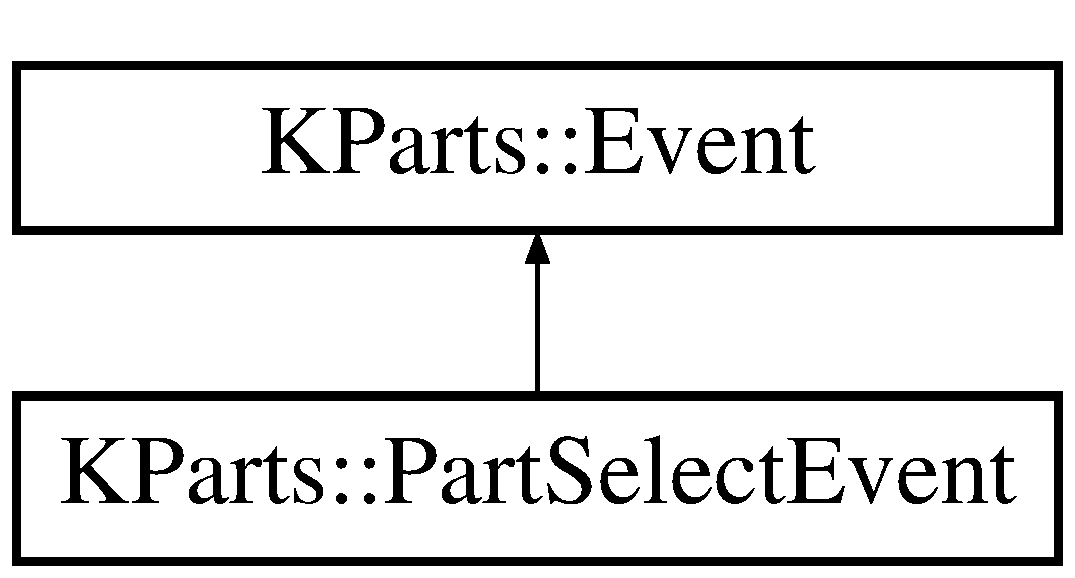
\includegraphics[height=2.000000cm]{classKParts_1_1PartSelectEvent}
\end{center}
\end{figure}
\subsection*{\-Public \-Member \-Functions}
\begin{DoxyCompactItemize}
\item 
\hyperlink{classKParts_1_1PartSelectEvent_ae31a4b63005a8e7493fd4fa5bd6f5e8d}{\-Part\-Select\-Event} (bool \hyperlink{classKParts_1_1PartSelectEvent_afbf342d865c918cdb6b856ab4168145f}{selected}, \hyperlink{classKParts_1_1Part}{\-Part} $\ast$\hyperlink{classKParts_1_1PartSelectEvent_a5e85934aca776852b1e8e25b01160f4e}{part}, \-Q\-Widget $\ast$\hyperlink{classKParts_1_1PartSelectEvent_a4f3b4a8544692181d2b49ffdeaad21d2}{widget})
\item 
virtual \hyperlink{classKParts_1_1PartSelectEvent_a5f1dc2753bd8a6a44a495fd6d505b312}{$\sim$\-Part\-Select\-Event} ()
\item 
bool \hyperlink{classKParts_1_1PartSelectEvent_afbf342d865c918cdb6b856ab4168145f}{selected} () const 
\item 
\hyperlink{classKParts_1_1Part}{\-Part} $\ast$ \hyperlink{classKParts_1_1PartSelectEvent_a5e85934aca776852b1e8e25b01160f4e}{part} () const 
\item 
\-Q\-Widget $\ast$ \hyperlink{classKParts_1_1PartSelectEvent_a4f3b4a8544692181d2b49ffdeaad21d2}{widget} () const 
\end{DoxyCompactItemize}
\subsection*{\-Static \-Public \-Member \-Functions}
\begin{DoxyCompactItemize}
\item 
static bool \hyperlink{classKParts_1_1PartSelectEvent_acc477c171d8bedc9e9cbcc23cf775024}{test} (const \-Q\-Event $\ast$event)
\end{DoxyCompactItemize}


\subsection{\-Detailed \-Description}
\-This event is sent when a part is selected or deselected. \begin{DoxySeeAlso}{\-See also}
\hyperlink{classKParts_1_1PartManager_a1b9382654eab488363d5f96364dee7ec}{\-K\-Parts\-::\-Part\-Manager\-::set\-Selection\-Policy} 
\end{DoxySeeAlso}


\-Definition at line 103 of file event.\-h.



\subsection{\-Constructor \& \-Destructor \-Documentation}
\hypertarget{classKParts_1_1PartSelectEvent_ae31a4b63005a8e7493fd4fa5bd6f5e8d}{\index{\-K\-Parts\-::\-Part\-Select\-Event@{\-K\-Parts\-::\-Part\-Select\-Event}!\-Part\-Select\-Event@{\-Part\-Select\-Event}}
\index{\-Part\-Select\-Event@{\-Part\-Select\-Event}!KParts::PartSelectEvent@{\-K\-Parts\-::\-Part\-Select\-Event}}
\subsubsection[{\-Part\-Select\-Event}]{\setlength{\rightskip}{0pt plus 5cm}{\bf \-K\-Parts\-::\-Part\-Select\-Event\-::\-Part\-Select\-Event} (
\begin{DoxyParamCaption}
\item[{bool}]{selected, }
\item[{{\bf \-Part} $\ast$}]{part, }
\item[{\-Q\-Widget $\ast$}]{widget}
\end{DoxyParamCaption}
)}}\label{classKParts_1_1PartSelectEvent_ae31a4b63005a8e7493fd4fa5bd6f5e8d}
\hypertarget{classKParts_1_1PartSelectEvent_a5f1dc2753bd8a6a44a495fd6d505b312}{\index{\-K\-Parts\-::\-Part\-Select\-Event@{\-K\-Parts\-::\-Part\-Select\-Event}!$\sim$\-Part\-Select\-Event@{$\sim$\-Part\-Select\-Event}}
\index{$\sim$\-Part\-Select\-Event@{$\sim$\-Part\-Select\-Event}!KParts::PartSelectEvent@{\-K\-Parts\-::\-Part\-Select\-Event}}
\subsubsection[{$\sim$\-Part\-Select\-Event}]{\setlength{\rightskip}{0pt plus 5cm}virtual {\bf \-K\-Parts\-::\-Part\-Select\-Event\-::$\sim$\-Part\-Select\-Event} (
\begin{DoxyParamCaption}
{}
\end{DoxyParamCaption}
)\hspace{0.3cm}{\ttfamily  \mbox{[}virtual\mbox{]}}}}\label{classKParts_1_1PartSelectEvent_a5f1dc2753bd8a6a44a495fd6d505b312}


\subsection{\-Member \-Function \-Documentation}
\hypertarget{classKParts_1_1PartSelectEvent_a5e85934aca776852b1e8e25b01160f4e}{\index{\-K\-Parts\-::\-Part\-Select\-Event@{\-K\-Parts\-::\-Part\-Select\-Event}!part@{part}}
\index{part@{part}!KParts::PartSelectEvent@{\-K\-Parts\-::\-Part\-Select\-Event}}
\subsubsection[{part}]{\setlength{\rightskip}{0pt plus 5cm}{\bf \-Part}$\ast$ {\bf \-K\-Parts\-::\-Part\-Select\-Event\-::part} (
\begin{DoxyParamCaption}
{}
\end{DoxyParamCaption}
) const}}\label{classKParts_1_1PartSelectEvent_a5e85934aca776852b1e8e25b01160f4e}
\hypertarget{classKParts_1_1PartSelectEvent_afbf342d865c918cdb6b856ab4168145f}{\index{\-K\-Parts\-::\-Part\-Select\-Event@{\-K\-Parts\-::\-Part\-Select\-Event}!selected@{selected}}
\index{selected@{selected}!KParts::PartSelectEvent@{\-K\-Parts\-::\-Part\-Select\-Event}}
\subsubsection[{selected}]{\setlength{\rightskip}{0pt plus 5cm}bool {\bf \-K\-Parts\-::\-Part\-Select\-Event\-::selected} (
\begin{DoxyParamCaption}
{}
\end{DoxyParamCaption}
) const}}\label{classKParts_1_1PartSelectEvent_afbf342d865c918cdb6b856ab4168145f}
\hypertarget{classKParts_1_1PartSelectEvent_acc477c171d8bedc9e9cbcc23cf775024}{\index{\-K\-Parts\-::\-Part\-Select\-Event@{\-K\-Parts\-::\-Part\-Select\-Event}!test@{test}}
\index{test@{test}!KParts::PartSelectEvent@{\-K\-Parts\-::\-Part\-Select\-Event}}
\subsubsection[{test}]{\setlength{\rightskip}{0pt plus 5cm}static bool {\bf \-K\-Parts\-::\-Part\-Select\-Event\-::test} (
\begin{DoxyParamCaption}
\item[{const \-Q\-Event $\ast$}]{event}
\end{DoxyParamCaption}
)\hspace{0.3cm}{\ttfamily  \mbox{[}static\mbox{]}}}}\label{classKParts_1_1PartSelectEvent_acc477c171d8bedc9e9cbcc23cf775024}


\-Reimplemented from \hyperlink{classKParts_1_1Event_a825b18534ae37dae24f2a2b326db0629}{\-K\-Parts\-::\-Event}.

\hypertarget{classKParts_1_1PartSelectEvent_a4f3b4a8544692181d2b49ffdeaad21d2}{\index{\-K\-Parts\-::\-Part\-Select\-Event@{\-K\-Parts\-::\-Part\-Select\-Event}!widget@{widget}}
\index{widget@{widget}!KParts::PartSelectEvent@{\-K\-Parts\-::\-Part\-Select\-Event}}
\subsubsection[{widget}]{\setlength{\rightskip}{0pt plus 5cm}\-Q\-Widget$\ast$ {\bf \-K\-Parts\-::\-Part\-Select\-Event\-::widget} (
\begin{DoxyParamCaption}
{}
\end{DoxyParamCaption}
) const}}\label{classKParts_1_1PartSelectEvent_a4f3b4a8544692181d2b49ffdeaad21d2}


\-The documentation for this class was generated from the following file\-:\begin{DoxyCompactItemize}
\item 
/usr/include/kparts/\hyperlink{event_8h}{event.\-h}\end{DoxyCompactItemize}

\hypertarget{classKParts_1_1Plugin}{\section{K\+Parts\+:\+:Plugin Class Reference}
\label{classKParts_1_1Plugin}\index{K\+Parts\+::\+Plugin@{K\+Parts\+::\+Plugin}}
}


{\ttfamily \#include $<$plugin.\+h$>$}

Inheritance diagram for K\+Parts\+:\+:Plugin\+:\begin{figure}[H]
\begin{center}
\leavevmode
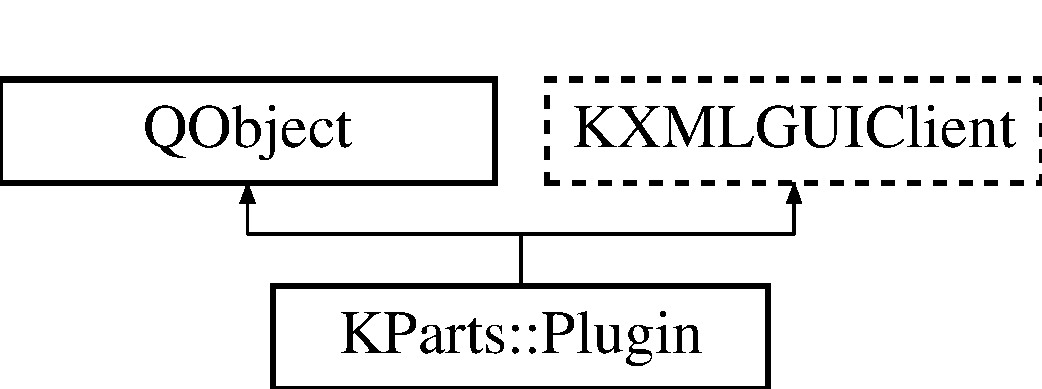
\includegraphics[height=2.000000cm]{classKParts_1_1Plugin}
\end{center}
\end{figure}
\subsection*{Classes}
\begin{DoxyCompactItemize}
\item 
struct \hyperlink{structKParts_1_1Plugin_1_1PluginInfo}{Plugin\+Info}
\end{DoxyCompactItemize}
\subsection*{Public Member Functions}
\begin{DoxyCompactItemize}
\item 
\hyperlink{classKParts_1_1Plugin_ab9f6924150a0a8ec941f4e81ba22311b}{Plugin} (Q\+Object $\ast$parent=0)
\item 
virtual \hyperlink{classKParts_1_1Plugin_a8a31c0e95c1a8c467a8f22f0da9022ff}{$\sim$\+Plugin} ()
\item 
virtual Q\+String \hyperlink{classKParts_1_1Plugin_aef2c9fe874cea1c76e17418fee2a0268}{xml\+File} () const 
\item 
virtual Q\+String \hyperlink{classKParts_1_1Plugin_a5d409b39746290ef1606840ea1cb15d8}{local\+X\+M\+L\+File} () const 
\end{DoxyCompactItemize}
\subsection*{Static Public Member Functions}
\begin{DoxyCompactItemize}
\item 
static void \hyperlink{classKParts_1_1Plugin_a66590bc55db365f880417d14f7ba38d0}{load\+Plugins} (Q\+Object $\ast$parent, const K\+Component\+Data \&instance)
\item 
static void \hyperlink{classKParts_1_1Plugin_a1634580342d43bf995041047e818f4a1}{load\+Plugins} (Q\+Object $\ast$parent, const \hyperlink{classQList}{Q\+List}$<$ \hyperlink{structKParts_1_1Plugin_1_1PluginInfo}{Plugin\+Info} $>$ \&\hyperlink{classKParts_1_1Plugin_a00fa7c83044416dbe32dcef7672fb7a5}{plugin\+Infos})
\item 
static void \hyperlink{classKParts_1_1Plugin_aef449c965dc8b644ed6502d7543891c7}{load\+Plugins} (Q\+Object $\ast$parent, const \hyperlink{classQList}{Q\+List}$<$ \hyperlink{structKParts_1_1Plugin_1_1PluginInfo}{Plugin\+Info} $>$ \&\hyperlink{classKParts_1_1Plugin_a00fa7c83044416dbe32dcef7672fb7a5}{plugin\+Infos}, const K\+Component\+Data \&instance)
\item 
static void \hyperlink{classKParts_1_1Plugin_a6f28c0e34f43edcc9cff5f6d474e8e01}{load\+Plugins} (Q\+Object $\ast$parent, K\+X\+M\+L\+G\+U\+I\+Client $\ast$parent\+G\+U\+I\+Client, const K\+Component\+Data \&instance, bool enable\+New\+Plugins\+By\+Default=true, int interface\+Version\+Required=0)
\item 
static \hyperlink{classQList}{Q\+List}$<$ \hyperlink{classKParts_1_1Plugin}{Plugin} $\ast$ $>$ \hyperlink{classKParts_1_1Plugin_ad53945bdaf59d6f0e1747c9106be9254}{plugin\+Objects} (Q\+Object $\ast$parent)
\end{DoxyCompactItemize}
\subsection*{Protected Member Functions}
\begin{DoxyCompactItemize}
\item 
virtual void \hyperlink{classKParts_1_1Plugin_a2406655ff0eb285c16516574cec136eb}{set\+Component\+Data} (const K\+Component\+Data \&instance)
\end{DoxyCompactItemize}
\subsection*{Static Protected Member Functions}
\begin{DoxyCompactItemize}
\item 
static \hyperlink{classQList}{Q\+List}$<$ \hyperlink{structKParts_1_1Plugin_1_1PluginInfo}{Plugin\+::\+Plugin\+Info} $>$ \hyperlink{classKParts_1_1Plugin_a00fa7c83044416dbe32dcef7672fb7a5}{plugin\+Infos} (const K\+Component\+Data \&instance)
\item 
static K\+D\+E\+\_\+\+D\+E\+P\+R\+E\+C\+A\+T\+E\+D \hyperlink{classKParts_1_1Plugin}{Plugin} $\ast$ \hyperlink{classKParts_1_1Plugin_adf61fe555a87f5ad3bf84c5e16a97e31}{load\+Plugin} (Q\+Object $\ast$parent, const char $\ast$libname)
\item 
static K\+D\+E\+\_\+\+D\+E\+P\+R\+E\+C\+A\+T\+E\+D \hyperlink{classKParts_1_1Plugin}{Plugin} $\ast$ \hyperlink{classKParts_1_1Plugin_a1479723a42f26aa8b4fd843e00976d5b}{load\+Plugin} (Q\+Object $\ast$parent, const Q\+Byte\+Array \&libname)
\item 
static \hyperlink{classKParts_1_1Plugin}{Plugin} $\ast$ \hyperlink{classKParts_1_1Plugin_ae2c2c4b6f736f5236bc5d4f2b20710a1}{load\+Plugin} (Q\+Object $\ast$parent, const Q\+String \&libname)
\item 
static \hyperlink{classKParts_1_1Plugin}{Plugin} $\ast$ \hyperlink{classKParts_1_1Plugin_a7fef84c255c7ed61b4548258fbaf3a68}{load\+Plugin} (Q\+Object $\ast$parent, const Q\+String \&libname, const Q\+String \&keyword)
\end{DoxyCompactItemize}


\subsection{Detailed Description}
A plugin is the way to add actions to an existing \hyperlink{namespaceKParts}{K\+Parts} application, or to a \hyperlink{classKParts_1_1Part}{Part}.

The X\+M\+L of those plugins looks exactly like of the shell or parts, with one small difference\+: The document tag should have an additional attribute, named \char`\"{}library\char`\"{}, and contain the name of the library implementing the plugin.

If you want this plugin to be used by a part, you need to install the rc file under the directory \char`\"{}data\char`\"{} (K\+D\+E\+D\+I\+R/share/apps usually)+\char`\"{}/instancename/kpartplugins/\char`\"{} where instancename is the name of the part's instance.

You should also install a \char`\"{}plugin info\char`\"{} .desktop file with the same name. \begin{DoxySeeAlso}{See Also}
K\+Plugin\+Info
\end{DoxySeeAlso}
For a tutorial on how to write plugins, see \href{http://developer.kde.org/documentation/tutorials/developing-a-plugin-structure/index.html#developing_plugins}{\tt http\+://developer.\+kde.\+org/documentation/tutorials/developing-\/a-\/plugin-\/structure/index.\+html\#developing\+\_\+plugins} 

Definition at line 54 of file plugin.\+h.



\subsection{Constructor \& Destructor Documentation}
\hypertarget{classKParts_1_1Plugin_ab9f6924150a0a8ec941f4e81ba22311b}{\index{K\+Parts\+::\+Plugin@{K\+Parts\+::\+Plugin}!Plugin@{Plugin}}
\index{Plugin@{Plugin}!K\+Parts\+::\+Plugin@{K\+Parts\+::\+Plugin}}
\subsubsection[{Plugin}]{\setlength{\rightskip}{0pt plus 5cm}K\+Parts\+::\+Plugin\+::\+Plugin (
\begin{DoxyParamCaption}
\item[{Q\+Object $\ast$}]{parent = {\ttfamily 0}}
\end{DoxyParamCaption}
)}}\label{classKParts_1_1Plugin_ab9f6924150a0a8ec941f4e81ba22311b}
Construct a new \hyperlink{namespaceKParts}{K\+Parts} plugin. \hypertarget{classKParts_1_1Plugin_a8a31c0e95c1a8c467a8f22f0da9022ff}{\index{K\+Parts\+::\+Plugin@{K\+Parts\+::\+Plugin}!````~Plugin@{$\sim$\+Plugin}}
\index{````~Plugin@{$\sim$\+Plugin}!K\+Parts\+::\+Plugin@{K\+Parts\+::\+Plugin}}
\subsubsection[{$\sim$\+Plugin}]{\setlength{\rightskip}{0pt plus 5cm}virtual K\+Parts\+::\+Plugin\+::$\sim$\+Plugin (
\begin{DoxyParamCaption}
{}
\end{DoxyParamCaption}
)\hspace{0.3cm}{\ttfamily [virtual]}}}\label{classKParts_1_1Plugin_a8a31c0e95c1a8c467a8f22f0da9022ff}
Destructor. 

\subsection{Member Function Documentation}
\hypertarget{classKParts_1_1Plugin_adf61fe555a87f5ad3bf84c5e16a97e31}{\index{K\+Parts\+::\+Plugin@{K\+Parts\+::\+Plugin}!load\+Plugin@{load\+Plugin}}
\index{load\+Plugin@{load\+Plugin}!K\+Parts\+::\+Plugin@{K\+Parts\+::\+Plugin}}
\subsubsection[{load\+Plugin}]{\setlength{\rightskip}{0pt plus 5cm}static K\+D\+E\+\_\+\+D\+E\+P\+R\+E\+C\+A\+T\+E\+D {\bf Plugin}$\ast$ K\+Parts\+::\+Plugin\+::load\+Plugin (
\begin{DoxyParamCaption}
\item[{Q\+Object $\ast$}]{parent, }
\item[{const char $\ast$}]{libname}
\end{DoxyParamCaption}
)\hspace{0.3cm}{\ttfamily [static]}, {\ttfamily [protected]}}}\label{classKParts_1_1Plugin_adf61fe555a87f5ad3bf84c5e16a97e31}
\hypertarget{classKParts_1_1Plugin_a1479723a42f26aa8b4fd843e00976d5b}{\index{K\+Parts\+::\+Plugin@{K\+Parts\+::\+Plugin}!load\+Plugin@{load\+Plugin}}
\index{load\+Plugin@{load\+Plugin}!K\+Parts\+::\+Plugin@{K\+Parts\+::\+Plugin}}
\subsubsection[{load\+Plugin}]{\setlength{\rightskip}{0pt plus 5cm}static K\+D\+E\+\_\+\+D\+E\+P\+R\+E\+C\+A\+T\+E\+D {\bf Plugin}$\ast$ K\+Parts\+::\+Plugin\+::load\+Plugin (
\begin{DoxyParamCaption}
\item[{Q\+Object $\ast$}]{parent, }
\item[{const Q\+Byte\+Array \&}]{libname}
\end{DoxyParamCaption}
)\hspace{0.3cm}{\ttfamily [static]}, {\ttfamily [protected]}}}\label{classKParts_1_1Plugin_a1479723a42f26aa8b4fd843e00976d5b}
\hypertarget{classKParts_1_1Plugin_ae2c2c4b6f736f5236bc5d4f2b20710a1}{\index{K\+Parts\+::\+Plugin@{K\+Parts\+::\+Plugin}!load\+Plugin@{load\+Plugin}}
\index{load\+Plugin@{load\+Plugin}!K\+Parts\+::\+Plugin@{K\+Parts\+::\+Plugin}}
\subsubsection[{load\+Plugin}]{\setlength{\rightskip}{0pt plus 5cm}static {\bf Plugin}$\ast$ K\+Parts\+::\+Plugin\+::load\+Plugin (
\begin{DoxyParamCaption}
\item[{Q\+Object $\ast$}]{parent, }
\item[{const Q\+String \&}]{libname}
\end{DoxyParamCaption}
)\hspace{0.3cm}{\ttfamily [static]}, {\ttfamily [protected]}}}\label{classKParts_1_1Plugin_ae2c2c4b6f736f5236bc5d4f2b20710a1}
\hypertarget{classKParts_1_1Plugin_a7fef84c255c7ed61b4548258fbaf3a68}{\index{K\+Parts\+::\+Plugin@{K\+Parts\+::\+Plugin}!load\+Plugin@{load\+Plugin}}
\index{load\+Plugin@{load\+Plugin}!K\+Parts\+::\+Plugin@{K\+Parts\+::\+Plugin}}
\subsubsection[{load\+Plugin}]{\setlength{\rightskip}{0pt plus 5cm}static {\bf Plugin}$\ast$ K\+Parts\+::\+Plugin\+::load\+Plugin (
\begin{DoxyParamCaption}
\item[{Q\+Object $\ast$}]{parent, }
\item[{const Q\+String \&}]{libname, }
\item[{const Q\+String \&}]{keyword}
\end{DoxyParamCaption}
)\hspace{0.3cm}{\ttfamily [static]}, {\ttfamily [protected]}}}\label{classKParts_1_1Plugin_a7fef84c255c7ed61b4548258fbaf3a68}
\hypertarget{classKParts_1_1Plugin_a66590bc55db365f880417d14f7ba38d0}{\index{K\+Parts\+::\+Plugin@{K\+Parts\+::\+Plugin}!load\+Plugins@{load\+Plugins}}
\index{load\+Plugins@{load\+Plugins}!K\+Parts\+::\+Plugin@{K\+Parts\+::\+Plugin}}
\subsubsection[{load\+Plugins}]{\setlength{\rightskip}{0pt plus 5cm}static void K\+Parts\+::\+Plugin\+::load\+Plugins (
\begin{DoxyParamCaption}
\item[{Q\+Object $\ast$}]{parent, }
\item[{const K\+Component\+Data \&}]{instance}
\end{DoxyParamCaption}
)\hspace{0.3cm}{\ttfamily [static]}}}\label{classKParts_1_1Plugin_a66590bc55db365f880417d14f7ba38d0}
Load the plugin libraries from the directories appropriate to {\ttfamily instance} and make the \hyperlink{classKParts_1_1Plugin}{Plugin} objects children of {\ttfamily parent}.

It is recommended to use the last load\+Plugins method instead, to support enabling and disabling of plugins. \hypertarget{classKParts_1_1Plugin_a1634580342d43bf995041047e818f4a1}{\index{K\+Parts\+::\+Plugin@{K\+Parts\+::\+Plugin}!load\+Plugins@{load\+Plugins}}
\index{load\+Plugins@{load\+Plugins}!K\+Parts\+::\+Plugin@{K\+Parts\+::\+Plugin}}
\subsubsection[{load\+Plugins}]{\setlength{\rightskip}{0pt plus 5cm}static void K\+Parts\+::\+Plugin\+::load\+Plugins (
\begin{DoxyParamCaption}
\item[{Q\+Object $\ast$}]{parent, }
\item[{const {\bf Q\+List}$<$ {\bf Plugin\+Info} $>$ \&}]{plugin\+Infos}
\end{DoxyParamCaption}
)\hspace{0.3cm}{\ttfamily [static]}}}\label{classKParts_1_1Plugin_a1634580342d43bf995041047e818f4a1}
Load the plugin libraries specified by the list {\ttfamily docs} and make the \hyperlink{classKParts_1_1Plugin}{Plugin} objects children of {\ttfamily parent} .

It is recommended to use the last load\+Plugins method instead, to support enabling and disabling of plugins. \hypertarget{classKParts_1_1Plugin_aef449c965dc8b644ed6502d7543891c7}{\index{K\+Parts\+::\+Plugin@{K\+Parts\+::\+Plugin}!load\+Plugins@{load\+Plugins}}
\index{load\+Plugins@{load\+Plugins}!K\+Parts\+::\+Plugin@{K\+Parts\+::\+Plugin}}
\subsubsection[{load\+Plugins}]{\setlength{\rightskip}{0pt plus 5cm}static void K\+Parts\+::\+Plugin\+::load\+Plugins (
\begin{DoxyParamCaption}
\item[{Q\+Object $\ast$}]{parent, }
\item[{const {\bf Q\+List}$<$ {\bf Plugin\+Info} $>$ \&}]{plugin\+Infos, }
\item[{const K\+Component\+Data \&}]{instance}
\end{DoxyParamCaption}
)\hspace{0.3cm}{\ttfamily [static]}}}\label{classKParts_1_1Plugin_aef449c965dc8b644ed6502d7543891c7}
Load the plugin libraries specified by the list {\ttfamily plugin\+Infos}, make the \hyperlink{classKParts_1_1Plugin}{Plugin} objects children of {\ttfamily parent}, and use the given {\ttfamily instance}.

It is recommended to use the last load\+Plugins method instead, to support enabling and disabling of plugins. \hypertarget{classKParts_1_1Plugin_a6f28c0e34f43edcc9cff5f6d474e8e01}{\index{K\+Parts\+::\+Plugin@{K\+Parts\+::\+Plugin}!load\+Plugins@{load\+Plugins}}
\index{load\+Plugins@{load\+Plugins}!K\+Parts\+::\+Plugin@{K\+Parts\+::\+Plugin}}
\subsubsection[{load\+Plugins}]{\setlength{\rightskip}{0pt plus 5cm}static void K\+Parts\+::\+Plugin\+::load\+Plugins (
\begin{DoxyParamCaption}
\item[{Q\+Object $\ast$}]{parent, }
\item[{K\+X\+M\+L\+G\+U\+I\+Client $\ast$}]{parent\+G\+U\+I\+Client, }
\item[{const K\+Component\+Data \&}]{instance, }
\item[{bool}]{enable\+New\+Plugins\+By\+Default = {\ttfamily true}, }
\item[{int}]{interface\+Version\+Required = {\ttfamily 0}}
\end{DoxyParamCaption}
)\hspace{0.3cm}{\ttfamily [static]}}}\label{classKParts_1_1Plugin_a6f28c0e34f43edcc9cff5f6d474e8e01}
Load the plugin libraries for the given {\ttfamily instance}, make the \hyperlink{classKParts_1_1Plugin}{Plugin} objects children of {\ttfamily parent}, and insert the plugin as a child G\+U\+I client of {\ttfamily parent\+G\+U\+I\+Client}.

This method uses the K\+Config object of the given instance, to find out which plugins are enabled and which are disabled. What happens by default (i.\+e. for new plugins that are not in that config file) is controlled by {\ttfamily enable\+New\+Plugins\+By\+Default}. It can be overridden by the plugin if it sets the X-\/\+K\+D\+E-\/\+Plugin\+Info-\/\+Enabled\+By\+Default key in the .desktop file (with the same name as the .rc file)

If a disabled plugin is already loaded it will be removed from the G\+U\+I factory and deleted.

If you change the binary interface offered by your part, you can avoid crashes from old plugins lying around by setting X-\/\+K\+D\+E-\/\+Interface\+Version=2 in the .desktop files of the plugins, and passing 2 to {\ttfamily interface\+Version\+Required}, so that the old plugins are not loaded. Increase both numbers every time a binary incompatible change in the application's plugin interface is made.

This method is automatically called by \hyperlink{classKParts_1_1Part}{K\+Parts\+::\+Part} and by \hyperlink{classKParts_1_1MainWindow}{K\+Parts\+::\+Main\+Window}. \begin{DoxySeeAlso}{See Also}
\hyperlink{classKParts_1_1PartBase_abaf6f9e33fa1890008905f9a1356e1a1}{Part\+Base\+::set\+Plugin\+Loading\+Mode}, \hyperlink{classKParts_1_1PartBase_a5a9ed59560edb848e787c4b3cee878b1}{Part\+Base\+::set\+Plugin\+Interface\+Version}
\end{DoxySeeAlso}
If you call this method in an already constructed G\+U\+I (like when the user has changed which plugins are enabled) you need to add the new plugins to the K\+X\+M\+L\+G\+U\+I\+Factory\+: 
\begin{DoxyCode}
\textcolor{keywordflow}{if}( factory() )
\{
  \textcolor{keyword}{const} \hyperlink{classQList}{QList<KParts::Plugin *>} plugins = 
      \hyperlink{classKParts_1_1Plugin_ad53945bdaf59d6f0e1747c9106be9254}{KParts::Plugin::pluginObjects}( \textcolor{keyword}{this} );
  \textcolor{keywordflow}{foreach} ( \hyperlink{classKParts_1_1Plugin}{KParts::Plugin} * plugin, plugins )
    factory()->addClient( plugin );
\}
\end{DoxyCode}
 \hypertarget{classKParts_1_1Plugin_a5d409b39746290ef1606840ea1cb15d8}{\index{K\+Parts\+::\+Plugin@{K\+Parts\+::\+Plugin}!local\+X\+M\+L\+File@{local\+X\+M\+L\+File}}
\index{local\+X\+M\+L\+File@{local\+X\+M\+L\+File}!K\+Parts\+::\+Plugin@{K\+Parts\+::\+Plugin}}
\subsubsection[{local\+X\+M\+L\+File}]{\setlength{\rightskip}{0pt plus 5cm}virtual Q\+String K\+Parts\+::\+Plugin\+::local\+X\+M\+L\+File (
\begin{DoxyParamCaption}
{}
\end{DoxyParamCaption}
) const\hspace{0.3cm}{\ttfamily [virtual]}}}\label{classKParts_1_1Plugin_a5d409b39746290ef1606840ea1cb15d8}
Reimplemented for internal reasons \hypertarget{classKParts_1_1Plugin_a00fa7c83044416dbe32dcef7672fb7a5}{\index{K\+Parts\+::\+Plugin@{K\+Parts\+::\+Plugin}!plugin\+Infos@{plugin\+Infos}}
\index{plugin\+Infos@{plugin\+Infos}!K\+Parts\+::\+Plugin@{K\+Parts\+::\+Plugin}}
\subsubsection[{plugin\+Infos}]{\setlength{\rightskip}{0pt plus 5cm}static {\bf Q\+List}$<${\bf Plugin\+::\+Plugin\+Info}$>$ K\+Parts\+::\+Plugin\+::plugin\+Infos (
\begin{DoxyParamCaption}
\item[{const K\+Component\+Data \&}]{instance}
\end{DoxyParamCaption}
)\hspace{0.3cm}{\ttfamily [static]}, {\ttfamily [protected]}}}\label{classKParts_1_1Plugin_a00fa7c83044416dbe32dcef7672fb7a5}
Look for plugins in the {\ttfamily instance's} \char`\"{}data\char`\"{} directory (+\char`\"{}/kpartplugins\char`\"{})

\begin{DoxyReturn}{Returns}
A list of Q\+Dom\+Document s, containing the parsed xml documents returned by plugins. 
\end{DoxyReturn}
\hypertarget{classKParts_1_1Plugin_ad53945bdaf59d6f0e1747c9106be9254}{\index{K\+Parts\+::\+Plugin@{K\+Parts\+::\+Plugin}!plugin\+Objects@{plugin\+Objects}}
\index{plugin\+Objects@{plugin\+Objects}!K\+Parts\+::\+Plugin@{K\+Parts\+::\+Plugin}}
\subsubsection[{plugin\+Objects}]{\setlength{\rightskip}{0pt plus 5cm}static {\bf Q\+List}$<${\bf Plugin} $\ast$$>$ K\+Parts\+::\+Plugin\+::plugin\+Objects (
\begin{DoxyParamCaption}
\item[{Q\+Object $\ast$}]{parent}
\end{DoxyParamCaption}
)\hspace{0.3cm}{\ttfamily [static]}}}\label{classKParts_1_1Plugin_ad53945bdaf59d6f0e1747c9106be9254}
Returns a list of plugin objects loaded for {\ttfamily parent}. This functions basically iterates over the children of the given object and returns those that inherit from \hyperlink{classKParts_1_1Plugin}{K\+Parts\+::\+Plugin}. \hypertarget{classKParts_1_1Plugin_a2406655ff0eb285c16516574cec136eb}{\index{K\+Parts\+::\+Plugin@{K\+Parts\+::\+Plugin}!set\+Component\+Data@{set\+Component\+Data}}
\index{set\+Component\+Data@{set\+Component\+Data}!K\+Parts\+::\+Plugin@{K\+Parts\+::\+Plugin}}
\subsubsection[{set\+Component\+Data}]{\setlength{\rightskip}{0pt plus 5cm}virtual void K\+Parts\+::\+Plugin\+::set\+Component\+Data (
\begin{DoxyParamCaption}
\item[{const K\+Component\+Data \&}]{instance}
\end{DoxyParamCaption}
)\hspace{0.3cm}{\ttfamily [protected]}, {\ttfamily [virtual]}}}\label{classKParts_1_1Plugin_a2406655ff0eb285c16516574cec136eb}
\hypertarget{classKParts_1_1Plugin_aef2c9fe874cea1c76e17418fee2a0268}{\index{K\+Parts\+::\+Plugin@{K\+Parts\+::\+Plugin}!xml\+File@{xml\+File}}
\index{xml\+File@{xml\+File}!K\+Parts\+::\+Plugin@{K\+Parts\+::\+Plugin}}
\subsubsection[{xml\+File}]{\setlength{\rightskip}{0pt plus 5cm}virtual Q\+String K\+Parts\+::\+Plugin\+::xml\+File (
\begin{DoxyParamCaption}
{}
\end{DoxyParamCaption}
) const\hspace{0.3cm}{\ttfamily [virtual]}}}\label{classKParts_1_1Plugin_aef2c9fe874cea1c76e17418fee2a0268}
Reimplemented for internal reasons 

The documentation for this class was generated from the following file\+:\begin{DoxyCompactItemize}
\item 
/usr/include/kparts/\hyperlink{plugin_8h}{plugin.\+h}\end{DoxyCompactItemize}

\hypertarget{structKParts_1_1Plugin_1_1PluginInfo}{\section{K\+Parts\+:\+:Plugin\+:\+:Plugin\+Info Struct Reference}
\label{structKParts_1_1Plugin_1_1PluginInfo}\index{K\+Parts\+::\+Plugin\+::\+Plugin\+Info@{K\+Parts\+::\+Plugin\+::\+Plugin\+Info}}
}


{\ttfamily \#include $<$plugin.\+h$>$}

\subsection*{Public Attributes}
\begin{DoxyCompactItemize}
\item 
Q\+String \hyperlink{structKParts_1_1Plugin_1_1PluginInfo_a02f9a1972d5e87b2d168fa7c5683649b}{m\+\_\+rel\+X\+M\+L\+File\+Name}
\item 
Q\+String \hyperlink{structKParts_1_1Plugin_1_1PluginInfo_a1351095a0ec3842ccf3c49cfd4c97478}{m\+\_\+abs\+X\+M\+L\+File\+Name}
\item 
Q\+Dom\+Document \hyperlink{structKParts_1_1Plugin_1_1PluginInfo_a5d8acab9612633d4d1f35019213ecadd}{m\+\_\+document}
\end{DoxyCompactItemize}


\subsection{Detailed Description}


Definition at line 58 of file plugin.\+h.



\subsection{Member Data Documentation}
\hypertarget{structKParts_1_1Plugin_1_1PluginInfo_a1351095a0ec3842ccf3c49cfd4c97478}{\index{K\+Parts\+::\+Plugin\+::\+Plugin\+Info@{K\+Parts\+::\+Plugin\+::\+Plugin\+Info}!m\+\_\+abs\+X\+M\+L\+File\+Name@{m\+\_\+abs\+X\+M\+L\+File\+Name}}
\index{m\+\_\+abs\+X\+M\+L\+File\+Name@{m\+\_\+abs\+X\+M\+L\+File\+Name}!K\+Parts\+::\+Plugin\+::\+Plugin\+Info@{K\+Parts\+::\+Plugin\+::\+Plugin\+Info}}
\subsubsection[{m\+\_\+abs\+X\+M\+L\+File\+Name}]{\setlength{\rightskip}{0pt plus 5cm}Q\+String K\+Parts\+::\+Plugin\+::\+Plugin\+Info\+::m\+\_\+abs\+X\+M\+L\+File\+Name}}\label{structKParts_1_1Plugin_1_1PluginInfo_a1351095a0ec3842ccf3c49cfd4c97478}


Definition at line 61 of file plugin.\+h.

\hypertarget{structKParts_1_1Plugin_1_1PluginInfo_a5d8acab9612633d4d1f35019213ecadd}{\index{K\+Parts\+::\+Plugin\+::\+Plugin\+Info@{K\+Parts\+::\+Plugin\+::\+Plugin\+Info}!m\+\_\+document@{m\+\_\+document}}
\index{m\+\_\+document@{m\+\_\+document}!K\+Parts\+::\+Plugin\+::\+Plugin\+Info@{K\+Parts\+::\+Plugin\+::\+Plugin\+Info}}
\subsubsection[{m\+\_\+document}]{\setlength{\rightskip}{0pt plus 5cm}Q\+Dom\+Document K\+Parts\+::\+Plugin\+::\+Plugin\+Info\+::m\+\_\+document}}\label{structKParts_1_1Plugin_1_1PluginInfo_a5d8acab9612633d4d1f35019213ecadd}


Definition at line 63 of file plugin.\+h.

\hypertarget{structKParts_1_1Plugin_1_1PluginInfo_a02f9a1972d5e87b2d168fa7c5683649b}{\index{K\+Parts\+::\+Plugin\+::\+Plugin\+Info@{K\+Parts\+::\+Plugin\+::\+Plugin\+Info}!m\+\_\+rel\+X\+M\+L\+File\+Name@{m\+\_\+rel\+X\+M\+L\+File\+Name}}
\index{m\+\_\+rel\+X\+M\+L\+File\+Name@{m\+\_\+rel\+X\+M\+L\+File\+Name}!K\+Parts\+::\+Plugin\+::\+Plugin\+Info@{K\+Parts\+::\+Plugin\+::\+Plugin\+Info}}
\subsubsection[{m\+\_\+rel\+X\+M\+L\+File\+Name}]{\setlength{\rightskip}{0pt plus 5cm}Q\+String K\+Parts\+::\+Plugin\+::\+Plugin\+Info\+::m\+\_\+rel\+X\+M\+L\+File\+Name}}\label{structKParts_1_1Plugin_1_1PluginInfo_a02f9a1972d5e87b2d168fa7c5683649b}


Definition at line 60 of file plugin.\+h.



The documentation for this struct was generated from the following file\+:\begin{DoxyCompactItemize}
\item 
/usr/include/kparts/\hyperlink{plugin_8h}{plugin.\+h}\end{DoxyCompactItemize}

\hypertarget{classKParts_1_1ReadOnlyPart}{\section{\-K\-Parts\-:\-:\-Read\-Only\-Part \-Class \-Reference}
\label{classKParts_1_1ReadOnlyPart}\index{\-K\-Parts\-::\-Read\-Only\-Part@{\-K\-Parts\-::\-Read\-Only\-Part}}
}


{\ttfamily \#include $<$part.\-h$>$}

\-Inheritance diagram for \-K\-Parts\-:\-:\-Read\-Only\-Part\-:\begin{figure}[H]
\begin{center}
\leavevmode
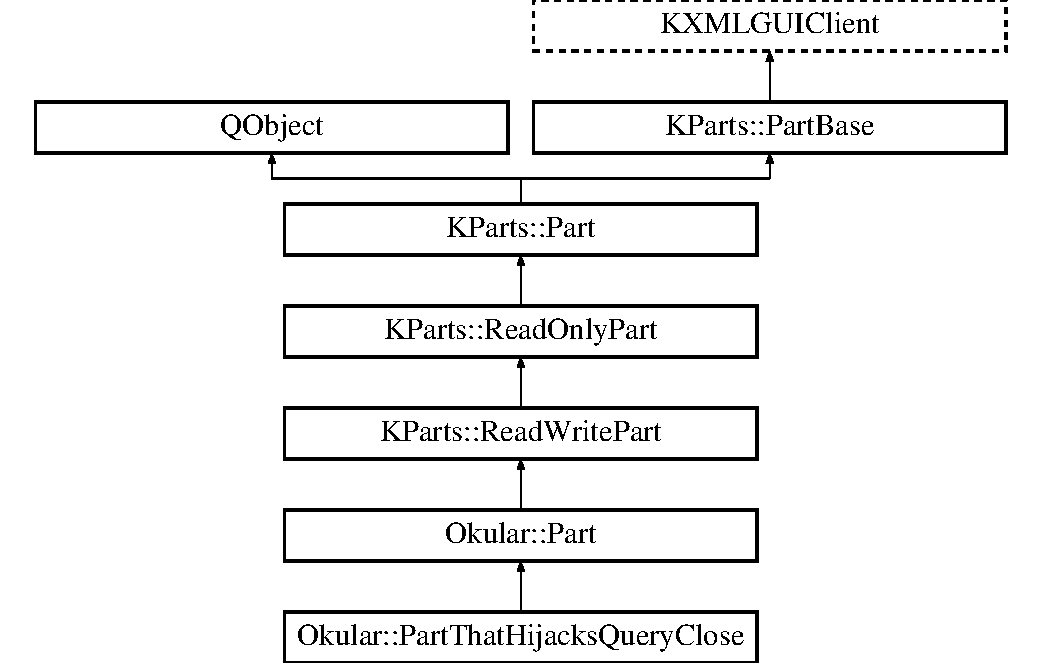
\includegraphics[height=4.000000cm]{classKParts_1_1ReadOnlyPart}
\end{center}
\end{figure}
\subsection*{\-Public \-Slots}
\begin{DoxyCompactItemize}
\item 
virtual bool \hyperlink{classKParts_1_1ReadOnlyPart_a1ff41b28f8da57ccc380e0c092a50c0c}{open\-Url} (const \-K\-Url \&\hyperlink{classKParts_1_1ReadOnlyPart_a5b8edbf05a338814287496882adde559}{url})
\end{DoxyCompactItemize}
\subsection*{\-Signals}
\begin{DoxyCompactItemize}
\item 
void \hyperlink{classKParts_1_1ReadOnlyPart_a1839e6f2741b7fca77cd4b04b5acdc6d}{started} (\-K\-I\-O\-::\-Job $\ast$)
\item 
void \hyperlink{classKParts_1_1ReadOnlyPart_a7dbe7a0dd64ed631d7d7fc763167de31}{completed} ()
\item 
void \hyperlink{classKParts_1_1ReadOnlyPart_a48ddc679f4b303102237f8e33b29c904}{completed} (bool pending\-Action)
\item 
void \hyperlink{classKParts_1_1ReadOnlyPart_ab1083f7c30e868d66e1f326b94851d8c}{canceled} (const \-Q\-String \&err\-Msg)
\end{DoxyCompactItemize}
\subsection*{\-Public \-Member \-Functions}
\begin{DoxyCompactItemize}
\item 
\hyperlink{classKParts_1_1ReadOnlyPart_ad8b7c3b0f0bc8303dc66c79d8ebc57e9}{\-Read\-Only\-Part} (\-Q\-Object $\ast$parent=0)
\item 
virtual \hyperlink{classKParts_1_1ReadOnlyPart_a8609199ca6addc35abf7f78b02e3236c}{$\sim$\-Read\-Only\-Part} ()
\item 
void \hyperlink{classKParts_1_1ReadOnlyPart_a95a547b488bc688035cffbd3df6f0b27}{set\-Progress\-Info\-Enabled} (bool show)
\item 
bool \hyperlink{classKParts_1_1ReadOnlyPart_aa1cff9c4698b9631d5bdd9f912f91568}{is\-Progress\-Info\-Enabled} () const 
\item 
void \hyperlink{classKParts_1_1ReadOnlyPart_ab3e6bd5d262b6b0b26acc003b2957c0b}{show\-Progress\-Info} (bool show)
\item 
\-K\-Url \hyperlink{classKParts_1_1ReadOnlyPart_aba05c3b2fd42dcfebc6585e4f746d2cb}{url} () const 
\item 
virtual bool \hyperlink{classKParts_1_1ReadOnlyPart_a1df069c3c0503f529dc9f0d7007f144d}{close\-Url} ()
\item 
\hyperlink{classKParts_1_1BrowserExtension}{\-Browser\-Extension} $\ast$ \hyperlink{classKParts_1_1ReadOnlyPart_a58d61ab4d2b2ed8d7944e1b02dbba0e2}{browser\-Extension} () const 
\item 
void \hyperlink{classKParts_1_1ReadOnlyPart_aab893a47747cad8bb29f1f95316140de}{set\-Arguments} (const \hyperlink{classKParts_1_1OpenUrlArguments}{\-Open\-Url\-Arguments} \&\hyperlink{classKParts_1_1ReadOnlyPart_a811e25200521dcf347bacb6be7ab8ecf}{arguments})
\item 
\hyperlink{classKParts_1_1OpenUrlArguments}{\-Open\-Url\-Arguments} \hyperlink{classKParts_1_1ReadOnlyPart_a811e25200521dcf347bacb6be7ab8ecf}{arguments} () const 
\item 
bool \hyperlink{classKParts_1_1ReadOnlyPart_aa3dacdfd6412d40f62ed75b02058b5e4}{open\-Stream} (const \-Q\-String \&mime\-Type, const \-K\-Url \&\hyperlink{classKParts_1_1ReadOnlyPart_a5b8edbf05a338814287496882adde559}{url})
\item 
bool \hyperlink{classKParts_1_1ReadOnlyPart_a5e6aac81ead43987e1711207b00878db}{write\-Stream} (const \-Q\-Byte\-Array \&data)
\item 
bool \hyperlink{classKParts_1_1ReadOnlyPart_a7af5ff9f593ee75dac30498ebf87c255}{close\-Stream} ()
\end{DoxyCompactItemize}
\subsection*{\-Protected \-Member \-Functions}
\begin{DoxyCompactItemize}
\item 
virtual bool \hyperlink{classKParts_1_1ReadOnlyPart_a951a032497fb94b092dfd4fd134db09b}{open\-File} ()
\item 
void \hyperlink{classKParts_1_1ReadOnlyPart_abcfbcbb7ae52b89cbb4844405e8e9b6e}{abort\-Load} ()
\item 
virtual void \hyperlink{classKParts_1_1ReadOnlyPart_aa5ac9f161aef38a92bbf25891746cac0}{gui\-Activate\-Event} (\hyperlink{classKParts_1_1GUIActivateEvent}{\-G\-U\-I\-Activate\-Event} $\ast$event)
\item 
\-K\-D\-E\-\_\-\-D\-E\-P\-R\-E\-C\-A\-T\-E\-D bool \hyperlink{classKParts_1_1ReadOnlyPart_ace00a87565affbcdb3318a14d73969a6}{is\-Local\-File\-Temporary} () const 
\item 
\-K\-D\-E\-\_\-\-D\-E\-P\-R\-E\-C\-A\-T\-E\-D void \hyperlink{classKParts_1_1ReadOnlyPart_a68ab78486399e688ee5ebe9fda0cf35b}{set\-Local\-File\-Temporary} (bool temp)
\item 
void \hyperlink{classKParts_1_1ReadOnlyPart_a2d64650f22a8b72d8c56ddec21717df9}{set\-Url} (const \-K\-Url \&\hyperlink{classKParts_1_1ReadOnlyPart_a5b8edbf05a338814287496882adde559}{url})
\item 
\-Q\-String \hyperlink{classKParts_1_1ReadOnlyPart_a9c411f8471de1a852c8595719d179946}{local\-File\-Path} () const 
\item 
void \hyperlink{classKParts_1_1ReadOnlyPart_a25c155283ba9ad06eeb8b1b203e49789}{set\-Local\-File\-Path} (const \-Q\-String \&\hyperlink{classKParts_1_1ReadOnlyPart_a9c411f8471de1a852c8595719d179946}{local\-File\-Path})
\item 
\hyperlink{classKParts_1_1ReadOnlyPart_a08c76aee8709e9956d79266ba02791ff}{\-Read\-Only\-Part} (\-Read\-Only\-Part\-Private \&dd, \-Q\-Object $\ast$parent)
\end{DoxyCompactItemize}
\subsection*{\-Properties}
\begin{DoxyCompactItemize}
\item 
\-K\-Url \hyperlink{classKParts_1_1ReadOnlyPart_a5b8edbf05a338814287496882adde559}{url}
\end{DoxyCompactItemize}


\subsection{\-Detailed \-Description}
\-Base class for any \char`\"{}viewer\char`\"{} part.

\-This class takes care of network transparency for you, in the simplest way (downloading to a temporary file, then letting the part load from the temporary file). \-To use the built-\/in network transparency, you only need to implement \hyperlink{classKParts_1_1ReadOnlyPart_a951a032497fb94b092dfd4fd134db09b}{open\-File()}, not \hyperlink{classKParts_1_1ReadOnlyPart_a1ff41b28f8da57ccc380e0c092a50c0c}{open\-Url()}.

\-To implement network transparency differently (e.\-g. for progressive loading, like a web browser does for instance), or to prevent network transparency (but why would you do that?), you can override \hyperlink{classKParts_1_1ReadOnlyPart_a1ff41b28f8da57ccc380e0c092a50c0c}{open\-Url()}.

\hyperlink{namespaceKParts}{\-K\-Parts} \-Application can use the signals to show feedback while the \-U\-R\-L is being loaded.

\hyperlink{classKParts_1_1ReadOnlyPart}{\-Read\-Only\-Part} handles the window caption by setting it to the current \-U\-R\-L (set in \hyperlink{classKParts_1_1ReadOnlyPart_a1ff41b28f8da57ccc380e0c092a50c0c}{open\-Url()}, and each time the part is activated). \-If you want another caption, set it in \hyperlink{classKParts_1_1ReadOnlyPart_a951a032497fb94b092dfd4fd134db09b}{open\-File()} and (if the part might ever be used with a part manager) in \hyperlink{classKParts_1_1ReadOnlyPart_aa5ac9f161aef38a92bbf25891746cac0}{gui\-Activate\-Event()} 

\-Definition at line 488 of file part.\-h.



\subsection{\-Constructor \& \-Destructor \-Documentation}
\hypertarget{classKParts_1_1ReadOnlyPart_ad8b7c3b0f0bc8303dc66c79d8ebc57e9}{\index{\-K\-Parts\-::\-Read\-Only\-Part@{\-K\-Parts\-::\-Read\-Only\-Part}!\-Read\-Only\-Part@{\-Read\-Only\-Part}}
\index{\-Read\-Only\-Part@{\-Read\-Only\-Part}!KParts::ReadOnlyPart@{\-K\-Parts\-::\-Read\-Only\-Part}}
\subsubsection[{\-Read\-Only\-Part}]{\setlength{\rightskip}{0pt plus 5cm}{\bf \-K\-Parts\-::\-Read\-Only\-Part\-::\-Read\-Only\-Part} (
\begin{DoxyParamCaption}
\item[{\-Q\-Object $\ast$}]{parent = {\ttfamily 0}}
\end{DoxyParamCaption}
)\hspace{0.3cm}{\ttfamily  \mbox{[}explicit\mbox{]}}}}\label{classKParts_1_1ReadOnlyPart_ad8b7c3b0f0bc8303dc66c79d8ebc57e9}
\-Constructor \-See also \hyperlink{classKParts_1_1Part}{\-Part} for the set\-X\-X\-X methods to call. \hypertarget{classKParts_1_1ReadOnlyPart_a8609199ca6addc35abf7f78b02e3236c}{\index{\-K\-Parts\-::\-Read\-Only\-Part@{\-K\-Parts\-::\-Read\-Only\-Part}!$\sim$\-Read\-Only\-Part@{$\sim$\-Read\-Only\-Part}}
\index{$\sim$\-Read\-Only\-Part@{$\sim$\-Read\-Only\-Part}!KParts::ReadOnlyPart@{\-K\-Parts\-::\-Read\-Only\-Part}}
\subsubsection[{$\sim$\-Read\-Only\-Part}]{\setlength{\rightskip}{0pt plus 5cm}virtual {\bf \-K\-Parts\-::\-Read\-Only\-Part\-::$\sim$\-Read\-Only\-Part} (
\begin{DoxyParamCaption}
{}
\end{DoxyParamCaption}
)\hspace{0.3cm}{\ttfamily  \mbox{[}virtual\mbox{]}}}}\label{classKParts_1_1ReadOnlyPart_a8609199ca6addc35abf7f78b02e3236c}
\-Destructor \hypertarget{classKParts_1_1ReadOnlyPart_a08c76aee8709e9956d79266ba02791ff}{\index{\-K\-Parts\-::\-Read\-Only\-Part@{\-K\-Parts\-::\-Read\-Only\-Part}!\-Read\-Only\-Part@{\-Read\-Only\-Part}}
\index{\-Read\-Only\-Part@{\-Read\-Only\-Part}!KParts::ReadOnlyPart@{\-K\-Parts\-::\-Read\-Only\-Part}}
\subsubsection[{\-Read\-Only\-Part}]{\setlength{\rightskip}{0pt plus 5cm}{\bf \-K\-Parts\-::\-Read\-Only\-Part\-::\-Read\-Only\-Part} (
\begin{DoxyParamCaption}
\item[{\-Read\-Only\-Part\-Private \&}]{dd, }
\item[{\-Q\-Object $\ast$}]{parent}
\end{DoxyParamCaption}
)\hspace{0.3cm}{\ttfamily  \mbox{[}protected\mbox{]}}}}\label{classKParts_1_1ReadOnlyPart_a08c76aee8709e9956d79266ba02791ff}


\subsection{\-Member \-Function \-Documentation}
\hypertarget{classKParts_1_1ReadOnlyPart_abcfbcbb7ae52b89cbb4844405e8e9b6e}{\index{\-K\-Parts\-::\-Read\-Only\-Part@{\-K\-Parts\-::\-Read\-Only\-Part}!abort\-Load@{abort\-Load}}
\index{abort\-Load@{abort\-Load}!KParts::ReadOnlyPart@{\-K\-Parts\-::\-Read\-Only\-Part}}
\subsubsection[{abort\-Load}]{\setlength{\rightskip}{0pt plus 5cm}void {\bf \-K\-Parts\-::\-Read\-Only\-Part\-::abort\-Load} (
\begin{DoxyParamCaption}
{}
\end{DoxyParamCaption}
)\hspace{0.3cm}{\ttfamily  \mbox{[}protected\mbox{]}}}}\label{classKParts_1_1ReadOnlyPart_abcfbcbb7ae52b89cbb4844405e8e9b6e}
\hypertarget{classKParts_1_1ReadOnlyPart_a811e25200521dcf347bacb6be7ab8ecf}{\index{\-K\-Parts\-::\-Read\-Only\-Part@{\-K\-Parts\-::\-Read\-Only\-Part}!arguments@{arguments}}
\index{arguments@{arguments}!KParts::ReadOnlyPart@{\-K\-Parts\-::\-Read\-Only\-Part}}
\subsubsection[{arguments}]{\setlength{\rightskip}{0pt plus 5cm}{\bf \-Open\-Url\-Arguments} {\bf \-K\-Parts\-::\-Read\-Only\-Part\-::arguments} (
\begin{DoxyParamCaption}
{}
\end{DoxyParamCaption}
) const}}\label{classKParts_1_1ReadOnlyPart_a811e25200521dcf347bacb6be7ab8ecf}
\begin{DoxyReturn}{\-Returns}
the arguments that were used to open this \-U\-R\-L. 
\end{DoxyReturn}
\hypertarget{classKParts_1_1ReadOnlyPart_a58d61ab4d2b2ed8d7944e1b02dbba0e2}{\index{\-K\-Parts\-::\-Read\-Only\-Part@{\-K\-Parts\-::\-Read\-Only\-Part}!browser\-Extension@{browser\-Extension}}
\index{browser\-Extension@{browser\-Extension}!KParts::ReadOnlyPart@{\-K\-Parts\-::\-Read\-Only\-Part}}
\subsubsection[{browser\-Extension}]{\setlength{\rightskip}{0pt plus 5cm}{\bf \-Browser\-Extension}$\ast$ {\bf \-K\-Parts\-::\-Read\-Only\-Part\-::browser\-Extension} (
\begin{DoxyParamCaption}
{}
\end{DoxyParamCaption}
) const}}\label{classKParts_1_1ReadOnlyPart_a58d61ab4d2b2ed8d7944e1b02dbba0e2}
\-This convenience method returns the browser\-Extension for this part, or 0 if there isn't any. \hypertarget{classKParts_1_1ReadOnlyPart_ab1083f7c30e868d66e1f326b94851d8c}{\index{\-K\-Parts\-::\-Read\-Only\-Part@{\-K\-Parts\-::\-Read\-Only\-Part}!canceled@{canceled}}
\index{canceled@{canceled}!KParts::ReadOnlyPart@{\-K\-Parts\-::\-Read\-Only\-Part}}
\subsubsection[{canceled}]{\setlength{\rightskip}{0pt plus 5cm}void {\bf \-K\-Parts\-::\-Read\-Only\-Part\-::canceled} (
\begin{DoxyParamCaption}
\item[{const \-Q\-String \&}]{err\-Msg}
\end{DoxyParamCaption}
)\hspace{0.3cm}{\ttfamily  \mbox{[}signal\mbox{]}}}}\label{classKParts_1_1ReadOnlyPart_ab1083f7c30e868d66e1f326b94851d8c}
\-Emit this if loading is canceled by the user or by an error. 
\begin{DoxyParams}{\-Parameters}
{\em err\-Msg} & the error message, empty if the user canceled the loading voluntarily. \\
\hline
\end{DoxyParams}
\hypertarget{classKParts_1_1ReadOnlyPart_a7af5ff9f593ee75dac30498ebf87c255}{\index{\-K\-Parts\-::\-Read\-Only\-Part@{\-K\-Parts\-::\-Read\-Only\-Part}!close\-Stream@{close\-Stream}}
\index{close\-Stream@{close\-Stream}!KParts::ReadOnlyPart@{\-K\-Parts\-::\-Read\-Only\-Part}}
\subsubsection[{close\-Stream}]{\setlength{\rightskip}{0pt plus 5cm}bool {\bf \-K\-Parts\-::\-Read\-Only\-Part\-::close\-Stream} (
\begin{DoxyParamCaption}
{}
\end{DoxyParamCaption}
)}}\label{classKParts_1_1ReadOnlyPart_a7af5ff9f593ee75dac30498ebf87c255}
\-Terminate the sending of data to the part. \-With some data types (text, html...) close\-Stream might never actually be called, in the case of continuous streams, for instance plain text or \-H\-T\-M\-L data. \hypertarget{classKParts_1_1ReadOnlyPart_a1df069c3c0503f529dc9f0d7007f144d}{\index{\-K\-Parts\-::\-Read\-Only\-Part@{\-K\-Parts\-::\-Read\-Only\-Part}!close\-Url@{close\-Url}}
\index{close\-Url@{close\-Url}!KParts::ReadOnlyPart@{\-K\-Parts\-::\-Read\-Only\-Part}}
\subsubsection[{close\-Url}]{\setlength{\rightskip}{0pt plus 5cm}virtual bool {\bf \-K\-Parts\-::\-Read\-Only\-Part\-::close\-Url} (
\begin{DoxyParamCaption}
{}
\end{DoxyParamCaption}
)\hspace{0.3cm}{\ttfamily  \mbox{[}virtual\mbox{]}}}}\label{classKParts_1_1ReadOnlyPart_a1df069c3c0503f529dc9f0d7007f144d}
\-Called when closing the current url (e.\-g. document), for instance when switching to another url (note that \hyperlink{classKParts_1_1ReadOnlyPart_a1ff41b28f8da57ccc380e0c092a50c0c}{open\-Url()} calls it automatically in this case). \-If the current \-U\-R\-L is not fully loaded yet, aborts loading. \-Deletes the temporary file used when the url is remote. \begin{DoxyReturn}{\-Returns}
always true, but the return value exists for reimplementations 
\end{DoxyReturn}


\-Reimplemented in \hyperlink{classKParts_1_1ReadWritePart_a45ed4bb6df997d6db0eae0d63f66b050}{\-K\-Parts\-::\-Read\-Write\-Part}.

\hypertarget{classKParts_1_1ReadOnlyPart_a7dbe7a0dd64ed631d7d7fc763167de31}{\index{\-K\-Parts\-::\-Read\-Only\-Part@{\-K\-Parts\-::\-Read\-Only\-Part}!completed@{completed}}
\index{completed@{completed}!KParts::ReadOnlyPart@{\-K\-Parts\-::\-Read\-Only\-Part}}
\subsubsection[{completed}]{\setlength{\rightskip}{0pt plus 5cm}void {\bf \-K\-Parts\-::\-Read\-Only\-Part\-::completed} (
\begin{DoxyParamCaption}
{}
\end{DoxyParamCaption}
)\hspace{0.3cm}{\ttfamily  \mbox{[}signal\mbox{]}}}}\label{classKParts_1_1ReadOnlyPart_a7dbe7a0dd64ed631d7d7fc763167de31}
\-Emit this when you have completed loading data. \-Hosting apps will want to know when the process of loading the data is finished, so that they can access the data when everything is loaded. \hypertarget{classKParts_1_1ReadOnlyPart_a48ddc679f4b303102237f8e33b29c904}{\index{\-K\-Parts\-::\-Read\-Only\-Part@{\-K\-Parts\-::\-Read\-Only\-Part}!completed@{completed}}
\index{completed@{completed}!KParts::ReadOnlyPart@{\-K\-Parts\-::\-Read\-Only\-Part}}
\subsubsection[{completed}]{\setlength{\rightskip}{0pt plus 5cm}void {\bf \-K\-Parts\-::\-Read\-Only\-Part\-::completed} (
\begin{DoxyParamCaption}
\item[{bool}]{pending\-Action}
\end{DoxyParamCaption}
)\hspace{0.3cm}{\ttfamily  \mbox{[}signal\mbox{]}}}}\label{classKParts_1_1ReadOnlyPart_a48ddc679f4b303102237f8e33b29c904}
\-Same as the above signal except it indicates whether there is a pending action to be executed on a delay timer. \-An example of this is the meta-\/refresh tags on web pages used to reload/redirect after a certain period of time. \-This signal is useful if you want to give the user the ability to cancel such pending actions.

{\ttfamily pending\-Action} true if a pending action exists, false otherwise. \hypertarget{classKParts_1_1ReadOnlyPart_aa5ac9f161aef38a92bbf25891746cac0}{\index{\-K\-Parts\-::\-Read\-Only\-Part@{\-K\-Parts\-::\-Read\-Only\-Part}!gui\-Activate\-Event@{gui\-Activate\-Event}}
\index{gui\-Activate\-Event@{gui\-Activate\-Event}!KParts::ReadOnlyPart@{\-K\-Parts\-::\-Read\-Only\-Part}}
\subsubsection[{gui\-Activate\-Event}]{\setlength{\rightskip}{0pt plus 5cm}virtual void {\bf \-K\-Parts\-::\-Read\-Only\-Part\-::gui\-Activate\-Event} (
\begin{DoxyParamCaption}
\item[{{\bf \-G\-U\-I\-Activate\-Event} $\ast$}]{event}
\end{DoxyParamCaption}
)\hspace{0.3cm}{\ttfamily  \mbox{[}protected, virtual\mbox{]}}}}\label{classKParts_1_1ReadOnlyPart_aa5ac9f161aef38a92bbf25891746cac0}
\-Reimplemented from \hyperlink{classKParts_1_1Part}{\-Part}, so that the window caption is set to the current url (decoded) when the part is activated \-This is the usual behavior in 99\% of the apps \-Reimplement if you don't like it -\/ test for event-\/$>$activated() !

\-Technical note \-: this is done with \hyperlink{classKParts_1_1GUIActivateEvent}{\-G\-U\-I\-Activate\-Event} and not with \hyperlink{classKParts_1_1PartActivateEvent}{\-Part\-Activate\-Event} because it's handled by the mainwindow (which gets the even after the \hyperlink{classKParts_1_1PartActivateEvent}{\-Part\-Activate\-Event} events have been sent) 

\-Reimplemented from \hyperlink{classKParts_1_1Part_a34b92f00459085ca7e05b7e8ee321347}{\-K\-Parts\-::\-Part}.

\hypertarget{classKParts_1_1ReadOnlyPart_ace00a87565affbcdb3318a14d73969a6}{\index{\-K\-Parts\-::\-Read\-Only\-Part@{\-K\-Parts\-::\-Read\-Only\-Part}!is\-Local\-File\-Temporary@{is\-Local\-File\-Temporary}}
\index{is\-Local\-File\-Temporary@{is\-Local\-File\-Temporary}!KParts::ReadOnlyPart@{\-K\-Parts\-::\-Read\-Only\-Part}}
\subsubsection[{is\-Local\-File\-Temporary}]{\setlength{\rightskip}{0pt plus 5cm}\-K\-D\-E\-\_\-\-D\-E\-P\-R\-E\-C\-A\-T\-E\-D bool {\bf \-K\-Parts\-::\-Read\-Only\-Part\-::is\-Local\-File\-Temporary} (
\begin{DoxyParamCaption}
{}
\end{DoxyParamCaption}
) const\hspace{0.3cm}{\ttfamily  \mbox{[}protected\mbox{]}}}}\label{classKParts_1_1ReadOnlyPart_ace00a87565affbcdb3318a14d73969a6}
\hypertarget{classKParts_1_1ReadOnlyPart_aa1cff9c4698b9631d5bdd9f912f91568}{\index{\-K\-Parts\-::\-Read\-Only\-Part@{\-K\-Parts\-::\-Read\-Only\-Part}!is\-Progress\-Info\-Enabled@{is\-Progress\-Info\-Enabled}}
\index{is\-Progress\-Info\-Enabled@{is\-Progress\-Info\-Enabled}!KParts::ReadOnlyPart@{\-K\-Parts\-::\-Read\-Only\-Part}}
\subsubsection[{is\-Progress\-Info\-Enabled}]{\setlength{\rightskip}{0pt plus 5cm}bool {\bf \-K\-Parts\-::\-Read\-Only\-Part\-::is\-Progress\-Info\-Enabled} (
\begin{DoxyParamCaption}
{}
\end{DoxyParamCaption}
) const}}\label{classKParts_1_1ReadOnlyPart_aa1cff9c4698b9631d5bdd9f912f91568}
\-Returns whether the part shows the progress info dialog used by internal \hyperlink{namespaceKIO}{\-K\-I\-O} job. \hypertarget{classKParts_1_1ReadOnlyPart_a9c411f8471de1a852c8595719d179946}{\index{\-K\-Parts\-::\-Read\-Only\-Part@{\-K\-Parts\-::\-Read\-Only\-Part}!local\-File\-Path@{local\-File\-Path}}
\index{local\-File\-Path@{local\-File\-Path}!KParts::ReadOnlyPart@{\-K\-Parts\-::\-Read\-Only\-Part}}
\subsubsection[{local\-File\-Path}]{\setlength{\rightskip}{0pt plus 5cm}\-Q\-String {\bf \-K\-Parts\-::\-Read\-Only\-Part\-::local\-File\-Path} (
\begin{DoxyParamCaption}
{}
\end{DoxyParamCaption}
) const\hspace{0.3cm}{\ttfamily  \mbox{[}protected\mbox{]}}}}\label{classKParts_1_1ReadOnlyPart_a9c411f8471de1a852c8595719d179946}
\-Returns the local file path associated with this part. \hypertarget{classKParts_1_1ReadOnlyPart_a951a032497fb94b092dfd4fd134db09b}{\index{\-K\-Parts\-::\-Read\-Only\-Part@{\-K\-Parts\-::\-Read\-Only\-Part}!open\-File@{open\-File}}
\index{open\-File@{open\-File}!KParts::ReadOnlyPart@{\-K\-Parts\-::\-Read\-Only\-Part}}
\subsubsection[{open\-File}]{\setlength{\rightskip}{0pt plus 5cm}virtual bool {\bf \-K\-Parts\-::\-Read\-Only\-Part\-::open\-File} (
\begin{DoxyParamCaption}
{}
\end{DoxyParamCaption}
)\hspace{0.3cm}{\ttfamily  \mbox{[}protected, virtual\mbox{]}}}}\label{classKParts_1_1ReadOnlyPart_a951a032497fb94b092dfd4fd134db09b}
\-If the part uses the standard implementation of \hyperlink{classKParts_1_1ReadOnlyPart_a1ff41b28f8da57ccc380e0c092a50c0c}{open\-Url()}, it must reimplement this, to open the local file. \-The default implementation is simply \{ return false; \} \hypertarget{classKParts_1_1ReadOnlyPart_aa3dacdfd6412d40f62ed75b02058b5e4}{\index{\-K\-Parts\-::\-Read\-Only\-Part@{\-K\-Parts\-::\-Read\-Only\-Part}!open\-Stream@{open\-Stream}}
\index{open\-Stream@{open\-Stream}!KParts::ReadOnlyPart@{\-K\-Parts\-::\-Read\-Only\-Part}}
\subsubsection[{open\-Stream}]{\setlength{\rightskip}{0pt plus 5cm}bool {\bf \-K\-Parts\-::\-Read\-Only\-Part\-::open\-Stream} (
\begin{DoxyParamCaption}
\item[{const \-Q\-String \&}]{mime\-Type, }
\item[{const \-K\-Url \&}]{url}
\end{DoxyParamCaption}
)}}\label{classKParts_1_1ReadOnlyPart_aa3dacdfd6412d40f62ed75b02058b5e4}
\-Initiate sending data to this part. \-This is an alternative to open\-Url, which allows the user of the part to load the data itself, and send it progressively to the part.


\begin{DoxyParams}{\-Parameters}
{\em mime\-Type} & the type of data that is going to be sent to this part. \\
\hline
{\em url} & the \-U\-R\-L representing this data. \-Although not directly used, every \hyperlink{classKParts_1_1ReadOnlyPart}{\-Read\-Only\-Part} has a \-U\-R\-L (see \hyperlink{classKParts_1_1ReadOnlyPart_a5b8edbf05a338814287496882adde559}{url()}), so this simply sets it. \\
\hline
\end{DoxyParams}
\begin{DoxyReturn}{\-Returns}
true if the part supports progressive loading and accepts data, false otherwise. 
\end{DoxyReturn}
\hypertarget{classKParts_1_1ReadOnlyPart_a1ff41b28f8da57ccc380e0c092a50c0c}{\index{\-K\-Parts\-::\-Read\-Only\-Part@{\-K\-Parts\-::\-Read\-Only\-Part}!open\-Url@{open\-Url}}
\index{open\-Url@{open\-Url}!KParts::ReadOnlyPart@{\-K\-Parts\-::\-Read\-Only\-Part}}
\subsubsection[{open\-Url}]{\setlength{\rightskip}{0pt plus 5cm}virtual bool {\bf \-K\-Parts\-::\-Read\-Only\-Part\-::open\-Url} (
\begin{DoxyParamCaption}
\item[{const \-K\-Url \&}]{url}
\end{DoxyParamCaption}
)\hspace{0.3cm}{\ttfamily  \mbox{[}virtual, slot\mbox{]}}}}\label{classKParts_1_1ReadOnlyPart_a1ff41b28f8da57ccc380e0c092a50c0c}
\-Only reimplement open\-Url if you don't want the network transparency support to download from the url into a temporary file (when the url isn't local). \-Otherwise, reimplement \hyperlink{classKParts_1_1ReadOnlyPart_a951a032497fb94b092dfd4fd134db09b}{open\-File()} only .

\-If you reimplement it, don't forget to set the caption, usually with emit set\-Window\-Caption( url.\-pretty\-Url() ); \hypertarget{classKParts_1_1ReadOnlyPart_aab893a47747cad8bb29f1f95316140de}{\index{\-K\-Parts\-::\-Read\-Only\-Part@{\-K\-Parts\-::\-Read\-Only\-Part}!set\-Arguments@{set\-Arguments}}
\index{set\-Arguments@{set\-Arguments}!KParts::ReadOnlyPart@{\-K\-Parts\-::\-Read\-Only\-Part}}
\subsubsection[{set\-Arguments}]{\setlength{\rightskip}{0pt plus 5cm}void {\bf \-K\-Parts\-::\-Read\-Only\-Part\-::set\-Arguments} (
\begin{DoxyParamCaption}
\item[{const {\bf \-Open\-Url\-Arguments} \&}]{arguments}
\end{DoxyParamCaption}
)}}\label{classKParts_1_1ReadOnlyPart_aab893a47747cad8bb29f1f95316140de}
\-Sets the arguments to use for the next open\-Url call. \hypertarget{classKParts_1_1ReadOnlyPart_a25c155283ba9ad06eeb8b1b203e49789}{\index{\-K\-Parts\-::\-Read\-Only\-Part@{\-K\-Parts\-::\-Read\-Only\-Part}!set\-Local\-File\-Path@{set\-Local\-File\-Path}}
\index{set\-Local\-File\-Path@{set\-Local\-File\-Path}!KParts::ReadOnlyPart@{\-K\-Parts\-::\-Read\-Only\-Part}}
\subsubsection[{set\-Local\-File\-Path}]{\setlength{\rightskip}{0pt plus 5cm}void {\bf \-K\-Parts\-::\-Read\-Only\-Part\-::set\-Local\-File\-Path} (
\begin{DoxyParamCaption}
\item[{const \-Q\-String \&}]{local\-File\-Path}
\end{DoxyParamCaption}
)\hspace{0.3cm}{\ttfamily  \mbox{[}protected\mbox{]}}}}\label{classKParts_1_1ReadOnlyPart_a25c155283ba9ad06eeb8b1b203e49789}
\-Sets the local file path associated with this part. \hypertarget{classKParts_1_1ReadOnlyPart_a68ab78486399e688ee5ebe9fda0cf35b}{\index{\-K\-Parts\-::\-Read\-Only\-Part@{\-K\-Parts\-::\-Read\-Only\-Part}!set\-Local\-File\-Temporary@{set\-Local\-File\-Temporary}}
\index{set\-Local\-File\-Temporary@{set\-Local\-File\-Temporary}!KParts::ReadOnlyPart@{\-K\-Parts\-::\-Read\-Only\-Part}}
\subsubsection[{set\-Local\-File\-Temporary}]{\setlength{\rightskip}{0pt plus 5cm}\-K\-D\-E\-\_\-\-D\-E\-P\-R\-E\-C\-A\-T\-E\-D void {\bf \-K\-Parts\-::\-Read\-Only\-Part\-::set\-Local\-File\-Temporary} (
\begin{DoxyParamCaption}
\item[{bool}]{temp}
\end{DoxyParamCaption}
)\hspace{0.3cm}{\ttfamily  \mbox{[}protected\mbox{]}}}}\label{classKParts_1_1ReadOnlyPart_a68ab78486399e688ee5ebe9fda0cf35b}
\hypertarget{classKParts_1_1ReadOnlyPart_a95a547b488bc688035cffbd3df6f0b27}{\index{\-K\-Parts\-::\-Read\-Only\-Part@{\-K\-Parts\-::\-Read\-Only\-Part}!set\-Progress\-Info\-Enabled@{set\-Progress\-Info\-Enabled}}
\index{set\-Progress\-Info\-Enabled@{set\-Progress\-Info\-Enabled}!KParts::ReadOnlyPart@{\-K\-Parts\-::\-Read\-Only\-Part}}
\subsubsection[{set\-Progress\-Info\-Enabled}]{\setlength{\rightskip}{0pt plus 5cm}void {\bf \-K\-Parts\-::\-Read\-Only\-Part\-::set\-Progress\-Info\-Enabled} (
\begin{DoxyParamCaption}
\item[{bool}]{show}
\end{DoxyParamCaption}
)}}\label{classKParts_1_1ReadOnlyPart_a95a547b488bc688035cffbd3df6f0b27}
\-Call this to turn off the progress info dialog used by the internal \hyperlink{namespaceKIO}{\-K\-I\-O} job. \-Use this if you provide another way of displaying progress info (e.\-g. a statusbar), using the signals emitted by this class, and/or those emitted by the \-Job given by started. \hypertarget{classKParts_1_1ReadOnlyPart_a2d64650f22a8b72d8c56ddec21717df9}{\index{\-K\-Parts\-::\-Read\-Only\-Part@{\-K\-Parts\-::\-Read\-Only\-Part}!set\-Url@{set\-Url}}
\index{set\-Url@{set\-Url}!KParts::ReadOnlyPart@{\-K\-Parts\-::\-Read\-Only\-Part}}
\subsubsection[{set\-Url}]{\setlength{\rightskip}{0pt plus 5cm}void {\bf \-K\-Parts\-::\-Read\-Only\-Part\-::set\-Url} (
\begin{DoxyParamCaption}
\item[{const \-K\-Url \&}]{url}
\end{DoxyParamCaption}
)\hspace{0.3cm}{\ttfamily  \mbox{[}protected\mbox{]}}}}\label{classKParts_1_1ReadOnlyPart_a2d64650f22a8b72d8c56ddec21717df9}
\-Sets the url associated with this part. \hypertarget{classKParts_1_1ReadOnlyPart_ab3e6bd5d262b6b0b26acc003b2957c0b}{\index{\-K\-Parts\-::\-Read\-Only\-Part@{\-K\-Parts\-::\-Read\-Only\-Part}!show\-Progress\-Info@{show\-Progress\-Info}}
\index{show\-Progress\-Info@{show\-Progress\-Info}!KParts::ReadOnlyPart@{\-K\-Parts\-::\-Read\-Only\-Part}}
\subsubsection[{show\-Progress\-Info}]{\setlength{\rightskip}{0pt plus 5cm}void {\bf \-K\-Parts\-::\-Read\-Only\-Part\-::show\-Progress\-Info} (
\begin{DoxyParamCaption}
\item[{bool}]{show}
\end{DoxyParamCaption}
)}}\label{classKParts_1_1ReadOnlyPart_ab3e6bd5d262b6b0b26acc003b2957c0b}
\hypertarget{classKParts_1_1ReadOnlyPart_a1839e6f2741b7fca77cd4b04b5acdc6d}{\index{\-K\-Parts\-::\-Read\-Only\-Part@{\-K\-Parts\-::\-Read\-Only\-Part}!started@{started}}
\index{started@{started}!KParts::ReadOnlyPart@{\-K\-Parts\-::\-Read\-Only\-Part}}
\subsubsection[{started}]{\setlength{\rightskip}{0pt plus 5cm}void {\bf \-K\-Parts\-::\-Read\-Only\-Part\-::started} (
\begin{DoxyParamCaption}
\item[{\-K\-I\-O\-::\-Job $\ast$}]{}
\end{DoxyParamCaption}
)\hspace{0.3cm}{\ttfamily  \mbox{[}signal\mbox{]}}}}\label{classKParts_1_1ReadOnlyPart_a1839e6f2741b7fca77cd4b04b5acdc6d}
\-The part emits this when starting data. \-If using a \-K\-I\-O\-::\-Job, it sets the job in the signal, so that progress information can be shown. \-Otherwise, job is 0. \hypertarget{classKParts_1_1ReadOnlyPart_aba05c3b2fd42dcfebc6585e4f746d2cb}{\index{\-K\-Parts\-::\-Read\-Only\-Part@{\-K\-Parts\-::\-Read\-Only\-Part}!url@{url}}
\index{url@{url}!KParts::ReadOnlyPart@{\-K\-Parts\-::\-Read\-Only\-Part}}
\subsubsection[{url}]{\setlength{\rightskip}{0pt plus 5cm}\-K\-Url {\bf \-K\-Parts\-::\-Read\-Only\-Part\-::url} (
\begin{DoxyParamCaption}
{}
\end{DoxyParamCaption}
) const}}\label{classKParts_1_1ReadOnlyPart_aba05c3b2fd42dcfebc6585e4f746d2cb}
\-Returns the \-U\-R\-L currently opened in this part.

\begin{DoxyReturn}{\-Returns}
\-The current \-U\-R\-L. 
\end{DoxyReturn}
\hypertarget{classKParts_1_1ReadOnlyPart_a5e6aac81ead43987e1711207b00878db}{\index{\-K\-Parts\-::\-Read\-Only\-Part@{\-K\-Parts\-::\-Read\-Only\-Part}!write\-Stream@{write\-Stream}}
\index{write\-Stream@{write\-Stream}!KParts::ReadOnlyPart@{\-K\-Parts\-::\-Read\-Only\-Part}}
\subsubsection[{write\-Stream}]{\setlength{\rightskip}{0pt plus 5cm}bool {\bf \-K\-Parts\-::\-Read\-Only\-Part\-::write\-Stream} (
\begin{DoxyParamCaption}
\item[{const \-Q\-Byte\-Array \&}]{data}
\end{DoxyParamCaption}
)}}\label{classKParts_1_1ReadOnlyPart_a5e6aac81ead43987e1711207b00878db}
\-Send some data to the part. open\-Stream must have been called previously, and must have returned true. \begin{DoxyReturn}{\-Returns}
true if the data was accepted by the part. \-If false is returned, the application should stop sending data, and doesn't have to call close\-Stream. 
\end{DoxyReturn}


\subsection{\-Property \-Documentation}
\hypertarget{classKParts_1_1ReadOnlyPart_a5b8edbf05a338814287496882adde559}{\index{\-K\-Parts\-::\-Read\-Only\-Part@{\-K\-Parts\-::\-Read\-Only\-Part}!url@{url}}
\index{url@{url}!KParts::ReadOnlyPart@{\-K\-Parts\-::\-Read\-Only\-Part}}
\subsubsection[{url}]{\setlength{\rightskip}{0pt plus 5cm}\-K\-Url {\bf \-K\-Parts\-::\-Read\-Only\-Part\-::url}\hspace{0.3cm}{\ttfamily  \mbox{[}read\mbox{]}}}}\label{classKParts_1_1ReadOnlyPart_a5b8edbf05a338814287496882adde559}


\-Definition at line 492 of file part.\-h.



\-The documentation for this class was generated from the following file\-:\begin{DoxyCompactItemize}
\item 
/usr/include/kparts/\hyperlink{part_8h}{part.\-h}\end{DoxyCompactItemize}

\hypertarget{classKParts_1_1ReadWritePart}{\section{K\+Parts\+:\+:Read\+Write\+Part Class Reference}
\label{classKParts_1_1ReadWritePart}\index{K\+Parts\+::\+Read\+Write\+Part@{K\+Parts\+::\+Read\+Write\+Part}}
}


{\ttfamily \#include $<$part.\+h$>$}

Inheritance diagram for K\+Parts\+:\+:Read\+Write\+Part\+:\begin{figure}[H]
\begin{center}
\leavevmode
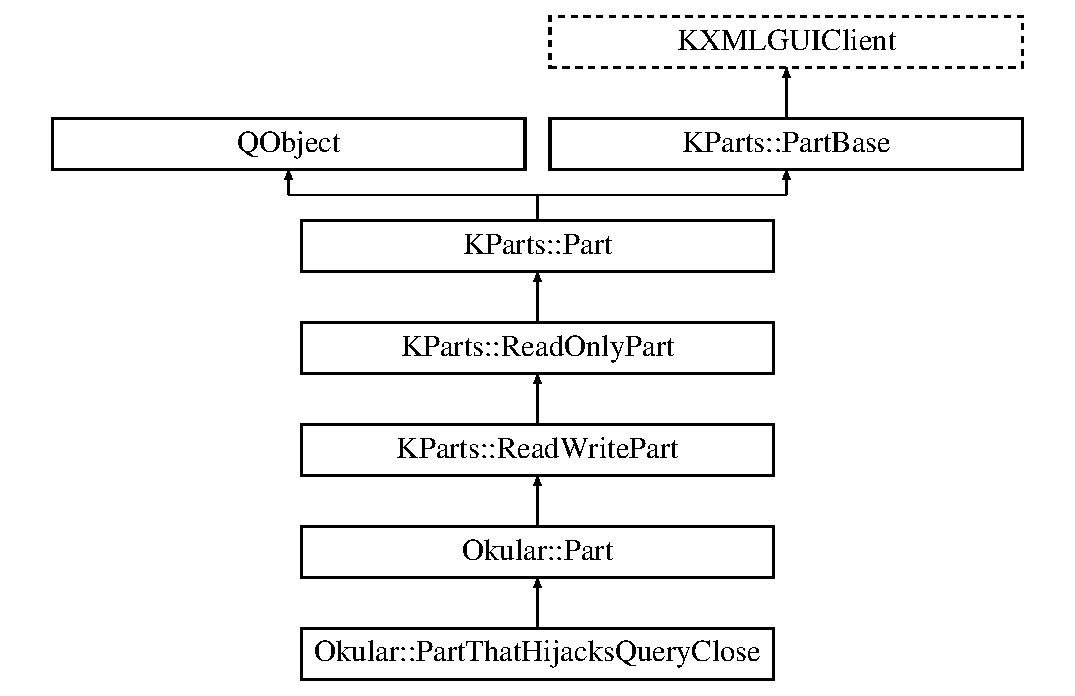
\includegraphics[height=7.000000cm]{classKParts_1_1ReadWritePart}
\end{center}
\end{figure}
\subsection*{Public Slots}
\begin{DoxyCompactItemize}
\item 
void \hyperlink{classKParts_1_1ReadWritePart_a3d3c236bfa46585c595eb8fca1f8b50a}{set\+Modified} ()
\item 
virtual bool \hyperlink{classKParts_1_1ReadWritePart_afcd2d898594f129e47ac4505c2ae5cd0}{save} ()
\item 
bool \hyperlink{classKParts_1_1ReadWritePart_a3c27f7fb8ee9636e2c9d6b5cd6328e49}{wait\+Save\+Complete} ()
\end{DoxyCompactItemize}
\subsection*{Signals}
\begin{DoxyCompactItemize}
\item 
void \hyperlink{classKParts_1_1ReadWritePart_adb7caee3c74e13b22dd922f67a68f830}{sig\+Query\+Close} (bool $\ast$handled, bool $\ast$abort\+Closing)
\end{DoxyCompactItemize}
\subsection*{Public Member Functions}
\begin{DoxyCompactItemize}
\item 
\hyperlink{classKParts_1_1ReadWritePart_a5444a248f62fa73ab6461dbbaed30054}{Read\+Write\+Part} (Q\+Object $\ast$parent=0)
\item 
virtual \hyperlink{classKParts_1_1ReadWritePart_a05e99804f15b4b8941fd026481cc74b2}{$\sim$\+Read\+Write\+Part} ()
\item 
bool \hyperlink{classKParts_1_1ReadWritePart_a1f77bd8acc3596f59cd07fa7918dafb1}{is\+Read\+Write} () const 
\item 
virtual void \hyperlink{classKParts_1_1ReadWritePart_a5b8c2d4b35739c882dc67f0acf8096c2}{set\+Read\+Write} (bool readwrite=true)
\item 
bool \hyperlink{classKParts_1_1ReadWritePart_a61acb87afb71c5cd7dcce295693e22e4}{is\+Modified} () const 
\item 
virtual bool \hyperlink{classKParts_1_1ReadWritePart_acdf38bc8da8b88a6ba38f9a3129d0c77}{query\+Close} ()
\item 
virtual bool \hyperlink{classKParts_1_1ReadWritePart_a45ed4bb6df997d6db0eae0d63f66b050}{close\+Url} ()
\item 
virtual bool \hyperlink{classKParts_1_1ReadWritePart_ac9d11b897ccf15ada8d15dd55eae3e3f}{close\+Url} (bool prompt\+To\+Save)
\item 
virtual bool \hyperlink{classKParts_1_1ReadWritePart_a5b10d70c83095f525b92fa5c9b554826}{save\+As} (const K\+Url \&\hyperlink{classKParts_1_1ReadOnlyPart_a5b8edbf05a338814287496882adde559}{url})
\item 
virtual void \hyperlink{classKParts_1_1ReadWritePart_ae8171d17ef8cf7f51a0607fa8a5df7d0}{set\+Modified} (bool modified)
\end{DoxyCompactItemize}
\subsection*{Protected Member Functions}
\begin{DoxyCompactItemize}
\item 
virtual bool \hyperlink{classKParts_1_1ReadWritePart_a599af24081c3dc1c261c04dce1de4f41}{save\+File} ()=0
\item 
virtual bool \hyperlink{classKParts_1_1ReadWritePart_affb719d6b8951cb1f3986b92db9527fe}{save\+To\+Url} ()
\end{DoxyCompactItemize}
\subsection*{Additional Inherited Members}


\subsection{Detailed Description}
Base class for an \char`\"{}editor\char`\"{} part.

This class handles network transparency for you. Anything that can open a U\+R\+L, allow modifications, and save (to the same U\+R\+L or a different one).

A read-\/write part can be set to read-\/only mode, using \hyperlink{classKParts_1_1ReadWritePart_a5b8c2d4b35739c882dc67f0acf8096c2}{set\+Read\+Write()}.

\hyperlink{classKParts_1_1Part}{Part} writers \+: Any part inheriting \hyperlink{classKParts_1_1ReadWritePart}{Read\+Write\+Part} should check is\+Read\+Write before allowing any action that modifies the part. The part probably wants to reimplement set\+Read\+Write, disable those actions. Don't forget to call the parent set\+Read\+Write. 

Definition at line 739 of file part.\+h.



\subsection{Constructor \& Destructor Documentation}
\hypertarget{classKParts_1_1ReadWritePart_a5444a248f62fa73ab6461dbbaed30054}{\index{K\+Parts\+::\+Read\+Write\+Part@{K\+Parts\+::\+Read\+Write\+Part}!Read\+Write\+Part@{Read\+Write\+Part}}
\index{Read\+Write\+Part@{Read\+Write\+Part}!K\+Parts\+::\+Read\+Write\+Part@{K\+Parts\+::\+Read\+Write\+Part}}
\subsubsection[{Read\+Write\+Part}]{\setlength{\rightskip}{0pt plus 5cm}K\+Parts\+::\+Read\+Write\+Part\+::\+Read\+Write\+Part (
\begin{DoxyParamCaption}
\item[{Q\+Object $\ast$}]{parent = {\ttfamily 0}}
\end{DoxyParamCaption}
)\hspace{0.3cm}{\ttfamily [explicit]}}}\label{classKParts_1_1ReadWritePart_a5444a248f62fa73ab6461dbbaed30054}
Constructor See parent constructor for instructions. \hypertarget{classKParts_1_1ReadWritePart_a05e99804f15b4b8941fd026481cc74b2}{\index{K\+Parts\+::\+Read\+Write\+Part@{K\+Parts\+::\+Read\+Write\+Part}!````~Read\+Write\+Part@{$\sim$\+Read\+Write\+Part}}
\index{````~Read\+Write\+Part@{$\sim$\+Read\+Write\+Part}!K\+Parts\+::\+Read\+Write\+Part@{K\+Parts\+::\+Read\+Write\+Part}}
\subsubsection[{$\sim$\+Read\+Write\+Part}]{\setlength{\rightskip}{0pt plus 5cm}virtual K\+Parts\+::\+Read\+Write\+Part\+::$\sim$\+Read\+Write\+Part (
\begin{DoxyParamCaption}
{}
\end{DoxyParamCaption}
)\hspace{0.3cm}{\ttfamily [virtual]}}}\label{classKParts_1_1ReadWritePart_a05e99804f15b4b8941fd026481cc74b2}
Destructor Applications using a \hyperlink{classKParts_1_1ReadWritePart}{Read\+Write\+Part} should make sure, before destroying it, to call \hyperlink{classKParts_1_1ReadWritePart_a45ed4bb6df997d6db0eae0d63f66b050}{close\+Url()}. In K\+Main\+Window\+::query\+Close(), for instance, they should allow closing only if the return value of \hyperlink{classKParts_1_1ReadWritePart_a45ed4bb6df997d6db0eae0d63f66b050}{close\+Url()} was true. This allows to cancel. 

\subsection{Member Function Documentation}
\hypertarget{classKParts_1_1ReadWritePart_a45ed4bb6df997d6db0eae0d63f66b050}{\index{K\+Parts\+::\+Read\+Write\+Part@{K\+Parts\+::\+Read\+Write\+Part}!close\+Url@{close\+Url}}
\index{close\+Url@{close\+Url}!K\+Parts\+::\+Read\+Write\+Part@{K\+Parts\+::\+Read\+Write\+Part}}
\subsubsection[{close\+Url}]{\setlength{\rightskip}{0pt plus 5cm}virtual bool K\+Parts\+::\+Read\+Write\+Part\+::close\+Url (
\begin{DoxyParamCaption}
{}
\end{DoxyParamCaption}
)\hspace{0.3cm}{\ttfamily [virtual]}}}\label{classKParts_1_1ReadWritePart_a45ed4bb6df997d6db0eae0d63f66b050}
Called when closing the current url (e.\+g. document), for instance when switching to another url (note that \hyperlink{classKParts_1_1ReadOnlyPart_a1ff41b28f8da57ccc380e0c092a50c0c}{open\+Url()} calls it automatically in this case).

If the current U\+R\+L is not fully loaded yet, aborts loading.

If \hyperlink{classKParts_1_1ReadWritePart_a61acb87afb71c5cd7dcce295693e22e4}{is\+Modified()}, \hyperlink{classKParts_1_1ReadWritePart_acdf38bc8da8b88a6ba38f9a3129d0c77}{query\+Close()} will be called.

\begin{DoxyReturn}{Returns}
false on cancel 
\end{DoxyReturn}


Reimplemented from \hyperlink{classKParts_1_1ReadOnlyPart_a1df069c3c0503f529dc9f0d7007f144d}{K\+Parts\+::\+Read\+Only\+Part}.



Reimplemented in \hyperlink{classOkular_1_1Part_a580d15b57647e05bf4b5d7674efc4dee}{Okular\+::\+Part}.

\hypertarget{classKParts_1_1ReadWritePart_ac9d11b897ccf15ada8d15dd55eae3e3f}{\index{K\+Parts\+::\+Read\+Write\+Part@{K\+Parts\+::\+Read\+Write\+Part}!close\+Url@{close\+Url}}
\index{close\+Url@{close\+Url}!K\+Parts\+::\+Read\+Write\+Part@{K\+Parts\+::\+Read\+Write\+Part}}
\subsubsection[{close\+Url}]{\setlength{\rightskip}{0pt plus 5cm}virtual bool K\+Parts\+::\+Read\+Write\+Part\+::close\+Url (
\begin{DoxyParamCaption}
\item[{bool}]{prompt\+To\+Save}
\end{DoxyParamCaption}
)\hspace{0.3cm}{\ttfamily [virtual]}}}\label{classKParts_1_1ReadWritePart_ac9d11b897ccf15ada8d15dd55eae3e3f}
Call this method instead of the above if you need control if the save prompt is shown. For example, if you call \hyperlink{classKParts_1_1ReadWritePart_acdf38bc8da8b88a6ba38f9a3129d0c77}{query\+Close()} from K\+Main\+Window\+::query\+Close(), you would not want to prompt again when closing the url.

Equivalent to prompt\+To\+Save ? \hyperlink{classKParts_1_1ReadWritePart_a45ed4bb6df997d6db0eae0d63f66b050}{close\+Url()} \+: \hyperlink{classKParts_1_1ReadOnlyPart_a1df069c3c0503f529dc9f0d7007f144d}{Read\+Only\+Part\+::close\+Url()} 

Reimplemented in \hyperlink{classOkular_1_1Part_ad4dc22f57f47a936614c58c352603a2a}{Okular\+::\+Part}.

\hypertarget{classKParts_1_1ReadWritePart_a61acb87afb71c5cd7dcce295693e22e4}{\index{K\+Parts\+::\+Read\+Write\+Part@{K\+Parts\+::\+Read\+Write\+Part}!is\+Modified@{is\+Modified}}
\index{is\+Modified@{is\+Modified}!K\+Parts\+::\+Read\+Write\+Part@{K\+Parts\+::\+Read\+Write\+Part}}
\subsubsection[{is\+Modified}]{\setlength{\rightskip}{0pt plus 5cm}bool K\+Parts\+::\+Read\+Write\+Part\+::is\+Modified (
\begin{DoxyParamCaption}
{}
\end{DoxyParamCaption}
) const}}\label{classKParts_1_1ReadWritePart_a61acb87afb71c5cd7dcce295693e22e4}
\begin{DoxyReturn}{Returns}
true if the document has been modified. 
\end{DoxyReturn}
\hypertarget{classKParts_1_1ReadWritePart_a1f77bd8acc3596f59cd07fa7918dafb1}{\index{K\+Parts\+::\+Read\+Write\+Part@{K\+Parts\+::\+Read\+Write\+Part}!is\+Read\+Write@{is\+Read\+Write}}
\index{is\+Read\+Write@{is\+Read\+Write}!K\+Parts\+::\+Read\+Write\+Part@{K\+Parts\+::\+Read\+Write\+Part}}
\subsubsection[{is\+Read\+Write}]{\setlength{\rightskip}{0pt plus 5cm}bool K\+Parts\+::\+Read\+Write\+Part\+::is\+Read\+Write (
\begin{DoxyParamCaption}
{}
\end{DoxyParamCaption}
) const}}\label{classKParts_1_1ReadWritePart_a1f77bd8acc3596f59cd07fa7918dafb1}
\begin{DoxyReturn}{Returns}
true if the part is in read-\/write mode 
\end{DoxyReturn}
\hypertarget{classKParts_1_1ReadWritePart_acdf38bc8da8b88a6ba38f9a3129d0c77}{\index{K\+Parts\+::\+Read\+Write\+Part@{K\+Parts\+::\+Read\+Write\+Part}!query\+Close@{query\+Close}}
\index{query\+Close@{query\+Close}!K\+Parts\+::\+Read\+Write\+Part@{K\+Parts\+::\+Read\+Write\+Part}}
\subsubsection[{query\+Close}]{\setlength{\rightskip}{0pt plus 5cm}virtual bool K\+Parts\+::\+Read\+Write\+Part\+::query\+Close (
\begin{DoxyParamCaption}
{}
\end{DoxyParamCaption}
)\hspace{0.3cm}{\ttfamily [virtual]}}}\label{classKParts_1_1ReadWritePart_acdf38bc8da8b88a6ba38f9a3129d0c77}
If the document has been modified, ask the user to save changes. This method is meant to be called from K\+Main\+Window\+::query\+Close(). It will also be called from \hyperlink{classKParts_1_1ReadWritePart_a45ed4bb6df997d6db0eae0d63f66b050}{close\+Url()}.

\begin{DoxyReturn}{Returns}
true if \hyperlink{classKParts_1_1ReadWritePart_a45ed4bb6df997d6db0eae0d63f66b050}{close\+Url()} can be called without the user losing important data, false if the user chooses to cancel. 
\end{DoxyReturn}


Reimplemented in \hyperlink{classOkular_1_1Part_a198e4caf3a79cea6e57be6e4b187152c}{Okular\+::\+Part}, and \hyperlink{classOkular_1_1PartThatHijacksQueryClose_acfbda56186d6f962dc8c9aa48eb935a8}{Okular\+::\+Part\+That\+Hijacks\+Query\+Close}.

\hypertarget{classKParts_1_1ReadWritePart_afcd2d898594f129e47ac4505c2ae5cd0}{\index{K\+Parts\+::\+Read\+Write\+Part@{K\+Parts\+::\+Read\+Write\+Part}!save@{save}}
\index{save@{save}!K\+Parts\+::\+Read\+Write\+Part@{K\+Parts\+::\+Read\+Write\+Part}}
\subsubsection[{save}]{\setlength{\rightskip}{0pt plus 5cm}virtual bool K\+Parts\+::\+Read\+Write\+Part\+::save (
\begin{DoxyParamCaption}
{}
\end{DoxyParamCaption}
)\hspace{0.3cm}{\ttfamily [virtual]}, {\ttfamily [slot]}}}\label{classKParts_1_1ReadWritePart_afcd2d898594f129e47ac4505c2ae5cd0}
Save the file in the location from which it was opened. You can connect this to the \char`\"{}save\char`\"{} action. Calls \hyperlink{classKParts_1_1ReadWritePart_a599af24081c3dc1c261c04dce1de4f41}{save\+File()} and \hyperlink{classKParts_1_1ReadWritePart_affb719d6b8951cb1f3986b92db9527fe}{save\+To\+Url()}, no need to reimplement. \hypertarget{classKParts_1_1ReadWritePart_a5b10d70c83095f525b92fa5c9b554826}{\index{K\+Parts\+::\+Read\+Write\+Part@{K\+Parts\+::\+Read\+Write\+Part}!save\+As@{save\+As}}
\index{save\+As@{save\+As}!K\+Parts\+::\+Read\+Write\+Part@{K\+Parts\+::\+Read\+Write\+Part}}
\subsubsection[{save\+As}]{\setlength{\rightskip}{0pt plus 5cm}virtual bool K\+Parts\+::\+Read\+Write\+Part\+::save\+As (
\begin{DoxyParamCaption}
\item[{const K\+Url \&}]{url}
\end{DoxyParamCaption}
)\hspace{0.3cm}{\ttfamily [virtual]}}}\label{classKParts_1_1ReadWritePart_a5b10d70c83095f525b92fa5c9b554826}
Save the file to a new location.

Calls \hyperlink{classKParts_1_1ReadWritePart_afcd2d898594f129e47ac4505c2ae5cd0}{save()}, no need to reimplement 

Reimplemented in \hyperlink{classOkular_1_1Part_a9041f15a5267877bc062131810811804}{Okular\+::\+Part}.

\hypertarget{classKParts_1_1ReadWritePart_a599af24081c3dc1c261c04dce1de4f41}{\index{K\+Parts\+::\+Read\+Write\+Part@{K\+Parts\+::\+Read\+Write\+Part}!save\+File@{save\+File}}
\index{save\+File@{save\+File}!K\+Parts\+::\+Read\+Write\+Part@{K\+Parts\+::\+Read\+Write\+Part}}
\subsubsection[{save\+File}]{\setlength{\rightskip}{0pt plus 5cm}virtual bool K\+Parts\+::\+Read\+Write\+Part\+::save\+File (
\begin{DoxyParamCaption}
{}
\end{DoxyParamCaption}
)\hspace{0.3cm}{\ttfamily [protected]}, {\ttfamily [pure virtual]}}}\label{classKParts_1_1ReadWritePart_a599af24081c3dc1c261c04dce1de4f41}
Save to a local file. You need to implement it, to save to the local file. The framework takes care of re-\/uploading afterwards.

\begin{DoxyReturn}{Returns}
true on success, false on failure. On failure the function should inform the user about the problem with an appropriate message box. Standard error messages can be constructed using K\+I\+O\+::build\+Error\+String() in combination with the error codes defined in kio/global.\+h 
\end{DoxyReturn}


Implemented in \hyperlink{classOkular_1_1Part_a92ed6a6fe1b4ab3c417bb96403a9eef0}{Okular\+::\+Part}.

\hypertarget{classKParts_1_1ReadWritePart_affb719d6b8951cb1f3986b92db9527fe}{\index{K\+Parts\+::\+Read\+Write\+Part@{K\+Parts\+::\+Read\+Write\+Part}!save\+To\+Url@{save\+To\+Url}}
\index{save\+To\+Url@{save\+To\+Url}!K\+Parts\+::\+Read\+Write\+Part@{K\+Parts\+::\+Read\+Write\+Part}}
\subsubsection[{save\+To\+Url}]{\setlength{\rightskip}{0pt plus 5cm}virtual bool K\+Parts\+::\+Read\+Write\+Part\+::save\+To\+Url (
\begin{DoxyParamCaption}
{}
\end{DoxyParamCaption}
)\hspace{0.3cm}{\ttfamily [protected]}, {\ttfamily [virtual]}}}\label{classKParts_1_1ReadWritePart_affb719d6b8951cb1f3986b92db9527fe}
Save the file.

Uploads the file, if {\ttfamily url} is remote. This will emit \hyperlink{classKParts_1_1ReadOnlyPart_a1839e6f2741b7fca77cd4b04b5acdc6d}{started()}, and either \hyperlink{classKParts_1_1ReadOnlyPart_a7dbe7a0dd64ed631d7d7fc763167de31}{completed()} or \hyperlink{classKParts_1_1ReadOnlyPart_ab1083f7c30e868d66e1f326b94851d8c}{canceled()}, in case you want to provide feedback. \begin{DoxyReturn}{Returns}
true on success, false on failure. 
\end{DoxyReturn}
\hypertarget{classKParts_1_1ReadWritePart_ae8171d17ef8cf7f51a0607fa8a5df7d0}{\index{K\+Parts\+::\+Read\+Write\+Part@{K\+Parts\+::\+Read\+Write\+Part}!set\+Modified@{set\+Modified}}
\index{set\+Modified@{set\+Modified}!K\+Parts\+::\+Read\+Write\+Part@{K\+Parts\+::\+Read\+Write\+Part}}
\subsubsection[{set\+Modified}]{\setlength{\rightskip}{0pt plus 5cm}virtual void K\+Parts\+::\+Read\+Write\+Part\+::set\+Modified (
\begin{DoxyParamCaption}
\item[{bool}]{modified}
\end{DoxyParamCaption}
)\hspace{0.3cm}{\ttfamily [virtual]}}}\label{classKParts_1_1ReadWritePart_ae8171d17ef8cf7f51a0607fa8a5df7d0}
Sets the modified flag of the part. \hypertarget{classKParts_1_1ReadWritePart_a3d3c236bfa46585c595eb8fca1f8b50a}{\index{K\+Parts\+::\+Read\+Write\+Part@{K\+Parts\+::\+Read\+Write\+Part}!set\+Modified@{set\+Modified}}
\index{set\+Modified@{set\+Modified}!K\+Parts\+::\+Read\+Write\+Part@{K\+Parts\+::\+Read\+Write\+Part}}
\subsubsection[{set\+Modified}]{\setlength{\rightskip}{0pt plus 5cm}void K\+Parts\+::\+Read\+Write\+Part\+::set\+Modified (
\begin{DoxyParamCaption}
{}
\end{DoxyParamCaption}
)\hspace{0.3cm}{\ttfamily [slot]}}}\label{classKParts_1_1ReadWritePart_a3d3c236bfa46585c595eb8fca1f8b50a}
Call \hyperlink{classKParts_1_1ReadWritePart_a3d3c236bfa46585c595eb8fca1f8b50a}{set\+Modified()} whenever the contents get modified. This is a slot for convenience, since it simply calls set\+Modified(true), so that you can connect it to a signal, like text\+Changed(). \hypertarget{classKParts_1_1ReadWritePart_a5b8c2d4b35739c882dc67f0acf8096c2}{\index{K\+Parts\+::\+Read\+Write\+Part@{K\+Parts\+::\+Read\+Write\+Part}!set\+Read\+Write@{set\+Read\+Write}}
\index{set\+Read\+Write@{set\+Read\+Write}!K\+Parts\+::\+Read\+Write\+Part@{K\+Parts\+::\+Read\+Write\+Part}}
\subsubsection[{set\+Read\+Write}]{\setlength{\rightskip}{0pt plus 5cm}virtual void K\+Parts\+::\+Read\+Write\+Part\+::set\+Read\+Write (
\begin{DoxyParamCaption}
\item[{bool}]{readwrite = {\ttfamily true}}
\end{DoxyParamCaption}
)\hspace{0.3cm}{\ttfamily [virtual]}}}\label{classKParts_1_1ReadWritePart_a5b8c2d4b35739c882dc67f0acf8096c2}
Changes the behavior of this part to readonly or readwrite. 
\begin{DoxyParams}{Parameters}
{\em readwrite} & set to true to enable readwrite mode \\
\hline
\end{DoxyParams}


Reimplemented in \hyperlink{classOkular_1_1Part_ae601c6c0ee3208c77233facdab9b0c9f}{Okular\+::\+Part}.

\hypertarget{classKParts_1_1ReadWritePart_adb7caee3c74e13b22dd922f67a68f830}{\index{K\+Parts\+::\+Read\+Write\+Part@{K\+Parts\+::\+Read\+Write\+Part}!sig\+Query\+Close@{sig\+Query\+Close}}
\index{sig\+Query\+Close@{sig\+Query\+Close}!K\+Parts\+::\+Read\+Write\+Part@{K\+Parts\+::\+Read\+Write\+Part}}
\subsubsection[{sig\+Query\+Close}]{\setlength{\rightskip}{0pt plus 5cm}void K\+Parts\+::\+Read\+Write\+Part\+::sig\+Query\+Close (
\begin{DoxyParamCaption}
\item[{bool $\ast$}]{handled, }
\item[{bool $\ast$}]{abort\+Closing}
\end{DoxyParamCaption}
)\hspace{0.3cm}{\ttfamily [signal]}}}\label{classKParts_1_1ReadWritePart_adb7caee3c74e13b22dd922f67a68f830}
set handled to true, if you don't want the default handling set abort\+Closing to true, if you handled the request, but for any reason don't want to allow closing the document \hypertarget{classKParts_1_1ReadWritePart_a3c27f7fb8ee9636e2c9d6b5cd6328e49}{\index{K\+Parts\+::\+Read\+Write\+Part@{K\+Parts\+::\+Read\+Write\+Part}!wait\+Save\+Complete@{wait\+Save\+Complete}}
\index{wait\+Save\+Complete@{wait\+Save\+Complete}!K\+Parts\+::\+Read\+Write\+Part@{K\+Parts\+::\+Read\+Write\+Part}}
\subsubsection[{wait\+Save\+Complete}]{\setlength{\rightskip}{0pt plus 5cm}bool K\+Parts\+::\+Read\+Write\+Part\+::wait\+Save\+Complete (
\begin{DoxyParamCaption}
{}
\end{DoxyParamCaption}
)\hspace{0.3cm}{\ttfamily [slot]}}}\label{classKParts_1_1ReadWritePart_a3c27f7fb8ee9636e2c9d6b5cd6328e49}
Waits for any pending upload job to finish and returns whether the last \hyperlink{classKParts_1_1ReadWritePart_afcd2d898594f129e47ac4505c2ae5cd0}{save()} action was successful. 

The documentation for this class was generated from the following file\+:\begin{DoxyCompactItemize}
\item 
/usr/include/kparts/\hyperlink{usr_2include_2kparts_2part_8h}{part.\+h}\end{DoxyCompactItemize}

\hypertarget{classKParts_1_1ScriptableExtension}{\section{\-K\-Parts\-:\-:\-Scriptable\-Extension \-Class \-Reference}
\label{classKParts_1_1ScriptableExtension}\index{\-K\-Parts\-::\-Scriptable\-Extension@{\-K\-Parts\-::\-Scriptable\-Extension}}
}


{\ttfamily \#include $<$scriptableextension.\-h$>$}

\subsection*{\-Classes}
\begin{DoxyCompactItemize}
\item 
struct \hyperlink{structKParts_1_1ScriptableExtension_1_1Exception}{\-Exception}
\item 
struct \hyperlink{structKParts_1_1ScriptableExtension_1_1FunctionRef}{\-Function\-Ref}
\item 
struct \hyperlink{structKParts_1_1ScriptableExtension_1_1Null}{\-Null}
\begin{DoxyCompactList}\small\item\em \-Corresponds to 'null' in \-Java\-Script. \end{DoxyCompactList}\item 
struct \hyperlink{structKParts_1_1ScriptableExtension_1_1Object}{\-Object}
\item 
struct \hyperlink{structKParts_1_1ScriptableExtension_1_1Undefined}{\-Undefined}
\begin{DoxyCompactList}\small\item\em \-Corresponds to 'undefined' in \-Java\-Script. \end{DoxyCompactList}\end{DoxyCompactItemize}
\subsection*{lifetime}
\begin{DoxyCompactItemize}
\item 
\hyperlink{classKParts_1_1ScriptableExtension_ab5aa7a70fe1b0643b5498529e574ef76}{\-Scriptable\-Extension} (\-Q\-Object $\ast$parent)
\item 
virtual \hyperlink{classKParts_1_1ScriptableExtension_aea7c940a43c9fba7279bc4d3a1959407}{$\sim$\-Scriptable\-Extension} ()
\item 
static \hyperlink{classKParts_1_1ScriptableExtension}{\-Scriptable\-Extension} $\ast$ \hyperlink{classKParts_1_1ScriptableExtension_a03e2028b730dbe724f27d97ff6422325}{child\-Object} (\-Q\-Object $\ast$obj)
\item 
static \hyperlink{classKParts_1_1ScriptableExtension}{\-Scriptable\-Extension} $\ast$ \hyperlink{classKParts_1_1ScriptableExtension_afe1e57b7a4ec5119d0d8eefff3ba6134}{adapter\-From\-Live\-Connect} (\-Q\-Object $\ast$parent\-Obj, \hyperlink{classKParts_1_1LiveConnectExtension}{\-Live\-Connect\-Extension} $\ast$old\-Api)
\end{DoxyCompactItemize}
\subsection*{\-Object \-Hierarchy}
\begin{DoxyCompactItemize}
\item 
void \hyperlink{classKParts_1_1ScriptableExtension_ac643fa084835c8fc07abd9072c1a079c}{set\-Host} (\hyperlink{classKParts_1_1ScriptableExtension}{\-Scriptable\-Extension} $\ast$\hyperlink{classKParts_1_1ScriptableExtension_a6505327b97b84ba5d5bae54664ee3ba6}{host})
\item 
\hyperlink{classKParts_1_1ScriptableExtension}{\-Scriptable\-Extension} $\ast$ \hyperlink{classKParts_1_1ScriptableExtension_a6505327b97b84ba5d5bae54664ee3ba6}{host} () const 
\item 
virtual \-Q\-Variant \hyperlink{classKParts_1_1ScriptableExtension_a2e74d0dce5db4528968dc545a73e22d6}{root\-Object} ()
\item 
\-Q\-Variant \hyperlink{classKParts_1_1ScriptableExtension_a1654d1f14b8f3184c4a2c4e382826aee}{enclosing\-Object} ()
\end{DoxyCompactItemize}
\subsection*{\-Object \-Operations}
\label{_amgrp60cb1b923af3b22f2c0b4823d5c6a3c1}%
 \-All these methods share the following conventions\-: \begin{DoxyItemize}
\item \-Values are passed and returned encoded as defined in \hyperlink{group__ScriptValueTypes}{\-Script \-Value \-Types} \item \-All methods may return an exception if unsupported \item \-All callers {\bfseries must} provide an accurate caller\-Principal argument describing which \hyperlink{classKParts_1_1ScriptableExtension}{\-Scriptable\-Extension} (and hence which \-K\-Part) they're acting as. \-This is used to implement {\bfseries security checks}. \-This is {\bfseries not} the same as the owner of an object. \-For example, if a plugin is calling an operation on a \-K\-H\-T\-M\-L\-Part object, then the 'this' parameter would be the object owner, a \hyperlink{classKParts_1_1ScriptableExtension}{\-Scriptable\-Extension} provided by the \-K\-H\-T\-M\-L\-Part, while the caller\-Principal would be the \hyperlink{classKParts_1_1ScriptableExtension}{\-Scriptable\-Extension} of the {\itshape plugin\/}. \-The extension is expected to do appropriate cross-\/site scripting checks on this argument if it is acting as a host. \end{DoxyItemize}
\begin{DoxyCompactItemize}
\item 
enum \hyperlink{classKParts_1_1ScriptableExtension_ae24e9c2e1e132201ddc092b8b069be23}{\-Script\-Language} \{ \hyperlink{classKParts_1_1ScriptableExtension_ae24e9c2e1e132201ddc092b8b069be23a53f57a3152be4d9428e8ee66c0614882}{\-E\-C\-M\-A\-Script}, 
\hyperlink{classKParts_1_1ScriptableExtension_ae24e9c2e1e132201ddc092b8b069be23a0609cfd03f0802c4af4ccae88f385f67}{\-Enum\-Limit} =  0x\-F\-F\-F\-F
 \}
\item 
typedef \-Q\-List$<$ \-Q\-Variant $>$ \hyperlink{classKParts_1_1ScriptableExtension_a6a35540990153f08b6dcf55d4b504c02}{\-Arg\-List}
\item 
virtual \-Q\-Variant \hyperlink{classKParts_1_1ScriptableExtension_a77efc2bc6776fd1e75b1e1a971eed643}{call\-As\-Function} (\hyperlink{classKParts_1_1ScriptableExtension}{\-Scriptable\-Extension} $\ast$caller\-Principal, quint64 obj\-Id, const \hyperlink{classKParts_1_1ScriptableExtension_a6a35540990153f08b6dcf55d4b504c02}{\-Arg\-List} \&args)
\item 
virtual \-Q\-Variant \hyperlink{classKParts_1_1ScriptableExtension_a5fa3ad1c1fe03543b0c03884dc71c8da}{call\-Function\-Reference} (\hyperlink{classKParts_1_1ScriptableExtension}{\-Scriptable\-Extension} $\ast$caller\-Principal, quint64 obj\-Id, const \-Q\-String \&f, const \hyperlink{classKParts_1_1ScriptableExtension_a6a35540990153f08b6dcf55d4b504c02}{\-Arg\-List} \&args)
\item 
virtual \-Q\-Variant \hyperlink{classKParts_1_1ScriptableExtension_a9cb5d813d297719d8ee00fa703ece547}{call\-As\-Constructor} (\hyperlink{classKParts_1_1ScriptableExtension}{\-Scriptable\-Extension} $\ast$caller\-Principal, quint64 obj\-Id, const \hyperlink{classKParts_1_1ScriptableExtension_a6a35540990153f08b6dcf55d4b504c02}{\-Arg\-List} \&args)
\item 
virtual bool \hyperlink{classKParts_1_1ScriptableExtension_a5f1fce8473702a961d49957c307e7e67}{has\-Property} (\hyperlink{classKParts_1_1ScriptableExtension}{\-Scriptable\-Extension} $\ast$caller\-Principal, quint64 obj\-Id, const \-Q\-String \&prop\-Name)
\item 
virtual \-Q\-Variant \hyperlink{classKParts_1_1ScriptableExtension_a90f5b0047ddb0b78096cab68a40c6326}{get} (\hyperlink{classKParts_1_1ScriptableExtension}{\-Scriptable\-Extension} $\ast$caller\-Principal, quint64 obj\-Id, const \-Q\-String \&prop\-Name)
\item 
virtual bool \hyperlink{classKParts_1_1ScriptableExtension_ad7cbeb6e9c0a92909e83d71e0646b5cd}{put} (\hyperlink{classKParts_1_1ScriptableExtension}{\-Scriptable\-Extension} $\ast$caller\-Principal, quint64 obj\-Id, const \-Q\-String \&prop\-Name, const \-Q\-Variant \&value)
\item 
virtual bool \hyperlink{classKParts_1_1ScriptableExtension_a72c9018ac01d931c4218ddbf963f93fb}{remove\-Property} (\hyperlink{classKParts_1_1ScriptableExtension}{\-Scriptable\-Extension} $\ast$caller\-Principal, quint64 obj\-Id, const \-Q\-String \&prop\-Name)
\item 
virtual bool \hyperlink{classKParts_1_1ScriptableExtension_a7630a47519df9f1ad5741e8d7cc436c2}{enumerate\-Properties} (\hyperlink{classKParts_1_1ScriptableExtension}{\-Scriptable\-Extension} $\ast$caller\-Principal, quint64 obj\-Id, \-Q\-String\-List $\ast$result)
\item 
virtual bool \hyperlink{classKParts_1_1ScriptableExtension_ac27156b3a945cb5ac69bbdfb18a501e8}{set\-Exception} (\hyperlink{classKParts_1_1ScriptableExtension}{\-Scriptable\-Extension} $\ast$caller\-Principal, const \-Q\-String \&message)
\item 
virtual \-Q\-Variant \hyperlink{classKParts_1_1ScriptableExtension_ae3ece3d86bd1410a0954e7dafc037d61}{evaluate\-Script} (\hyperlink{classKParts_1_1ScriptableExtension}{\-Scriptable\-Extension} $\ast$caller\-Principal, quint64 context\-Object\-Id, const \-Q\-String \&code, \hyperlink{classKParts_1_1ScriptableExtension_ae24e9c2e1e132201ddc092b8b069be23}{\-Script\-Language} language=\hyperlink{classKParts_1_1ScriptableExtension_ae24e9c2e1e132201ddc092b8b069be23a53f57a3152be4d9428e8ee66c0614882}{\-E\-C\-M\-A\-Script})
\item 
virtual bool \hyperlink{classKParts_1_1ScriptableExtension_adc8ddc26449ab07abdf05dab5fb06af1}{is\-Script\-Language\-Supported} (\hyperlink{classKParts_1_1ScriptableExtension_ae24e9c2e1e132201ddc092b8b069be23}{\-Script\-Language} lang) const 
\item 
virtual void \hyperlink{classKParts_1_1ScriptableExtension_aa9d21d12e60a00fa4adb0a3db0f52cad}{acquire} (quint64 objid)
\item 
virtual void \hyperlink{classKParts_1_1ScriptableExtension_a1a06fcb64081a052d29baae2376c371b}{release} (quint64 objid)
\item 
static \-Q\-Variant \hyperlink{classKParts_1_1ScriptableExtension_a048b779677ccf0e99e90b101281d31bc}{acquire\-Value} (const \-Q\-Variant \&v)
\item 
static \-Q\-Variant \hyperlink{classKParts_1_1ScriptableExtension_a45af0ab34d52c57452910b6161922c3c}{release\-Value} (const \-Q\-Variant \&v)
\end{DoxyCompactItemize}


\subsection{\-Detailed \-Description}
\-An extension class that permits \hyperlink{namespaceKParts}{\-K\-Parts} to be scripted (such as when embedded inside a \-K\-H\-T\-M\-L\-Part) and to access the host's scriptable objects as well.

\-See \hyperlink{group__ScriptValueTypes}{\-Script \-Value \-Types} for how values are passed to/from various methods here.

\begin{DoxySince}{\-Since}
4.\-5 
\end{DoxySince}


\-Definition at line 44 of file scriptableextension.\-h.



\subsection{\-Member \-Typedef \-Documentation}
\hypertarget{classKParts_1_1ScriptableExtension_a6a35540990153f08b6dcf55d4b504c02}{\index{\-K\-Parts\-::\-Scriptable\-Extension@{\-K\-Parts\-::\-Scriptable\-Extension}!\-Arg\-List@{\-Arg\-List}}
\index{\-Arg\-List@{\-Arg\-List}!KParts::ScriptableExtension@{\-K\-Parts\-::\-Scriptable\-Extension}}
\subsubsection[{\-Arg\-List}]{\setlength{\rightskip}{0pt plus 5cm}typedef \-Q\-List$<$\-Q\-Variant$>$ {\bf \-K\-Parts\-::\-Scriptable\-Extension\-::\-Arg\-List}}}\label{classKParts_1_1ScriptableExtension_a6a35540990153f08b6dcf55d4b504c02}


\-Definition at line 192 of file scriptableextension.\-h.



\subsection{\-Member \-Enumeration \-Documentation}
\hypertarget{classKParts_1_1ScriptableExtension_ae24e9c2e1e132201ddc092b8b069be23}{\index{\-K\-Parts\-::\-Scriptable\-Extension@{\-K\-Parts\-::\-Scriptable\-Extension}!\-Script\-Language@{\-Script\-Language}}
\index{\-Script\-Language@{\-Script\-Language}!KParts::ScriptableExtension@{\-K\-Parts\-::\-Scriptable\-Extension}}
\subsubsection[{\-Script\-Language}]{\setlength{\rightskip}{0pt plus 5cm}enum {\bf \-K\-Parts\-::\-Scriptable\-Extension\-::\-Script\-Language}}}\label{classKParts_1_1ScriptableExtension_ae24e9c2e1e132201ddc092b8b069be23}
\begin{Desc}
\item[\-Enumerator\-: ]\par
\begin{description}
\index{\-E\-C\-M\-A\-Script@{\-E\-C\-M\-A\-Script}!\-K\-Parts\-::\-Scriptable\-Extension@{\-K\-Parts\-::\-Scriptable\-Extension}}\index{\-K\-Parts\-::\-Scriptable\-Extension@{\-K\-Parts\-::\-Scriptable\-Extension}!\-E\-C\-M\-A\-Script@{\-E\-C\-M\-A\-Script}}\item[{\em 
\hypertarget{classKParts_1_1ScriptableExtension_ae24e9c2e1e132201ddc092b8b069be23a53f57a3152be4d9428e8ee66c0614882}{\-E\-C\-M\-A\-Script}\label{classKParts_1_1ScriptableExtension_ae24e9c2e1e132201ddc092b8b069be23a53f57a3152be4d9428e8ee66c0614882}
}]\index{\-Enum\-Limit@{\-Enum\-Limit}!\-K\-Parts\-::\-Scriptable\-Extension@{\-K\-Parts\-::\-Scriptable\-Extension}}\index{\-K\-Parts\-::\-Scriptable\-Extension@{\-K\-Parts\-::\-Scriptable\-Extension}!\-Enum\-Limit@{\-Enum\-Limit}}\item[{\em 
\hypertarget{classKParts_1_1ScriptableExtension_ae24e9c2e1e132201ddc092b8b069be23a0609cfd03f0802c4af4ccae88f385f67}{\-Enum\-Limit}\label{classKParts_1_1ScriptableExtension_ae24e9c2e1e132201ddc092b8b069be23a0609cfd03f0802c4af4ccae88f385f67}
}]$<$ also known as \-Java\-Script \end{description}
\end{Desc}



\-Definition at line 247 of file scriptableextension.\-h.


\begin{DoxyCode}
                        {
        ECMAScript, 
        EnumLimit = 0xFFFF
    };
\end{DoxyCode}


\subsection{\-Constructor \& \-Destructor \-Documentation}
\hypertarget{classKParts_1_1ScriptableExtension_ab5aa7a70fe1b0643b5498529e574ef76}{\index{\-K\-Parts\-::\-Scriptable\-Extension@{\-K\-Parts\-::\-Scriptable\-Extension}!\-Scriptable\-Extension@{\-Scriptable\-Extension}}
\index{\-Scriptable\-Extension@{\-Scriptable\-Extension}!KParts::ScriptableExtension@{\-K\-Parts\-::\-Scriptable\-Extension}}
\subsubsection[{\-Scriptable\-Extension}]{\setlength{\rightskip}{0pt plus 5cm}{\bf \-K\-Parts\-::\-Scriptable\-Extension\-::\-Scriptable\-Extension} (
\begin{DoxyParamCaption}
\item[{\-Q\-Object $\ast$}]{parent}
\end{DoxyParamCaption}
)\hspace{0.3cm}{\ttfamily  \mbox{[}protected\mbox{]}}}}\label{classKParts_1_1ScriptableExtension_ab5aa7a70fe1b0643b5498529e574ef76}
\hypertarget{classKParts_1_1ScriptableExtension_aea7c940a43c9fba7279bc4d3a1959407}{\index{\-K\-Parts\-::\-Scriptable\-Extension@{\-K\-Parts\-::\-Scriptable\-Extension}!$\sim$\-Scriptable\-Extension@{$\sim$\-Scriptable\-Extension}}
\index{$\sim$\-Scriptable\-Extension@{$\sim$\-Scriptable\-Extension}!KParts::ScriptableExtension@{\-K\-Parts\-::\-Scriptable\-Extension}}
\subsubsection[{$\sim$\-Scriptable\-Extension}]{\setlength{\rightskip}{0pt plus 5cm}virtual {\bf \-K\-Parts\-::\-Scriptable\-Extension\-::$\sim$\-Scriptable\-Extension} (
\begin{DoxyParamCaption}
{}
\end{DoxyParamCaption}
)\hspace{0.3cm}{\ttfamily  \mbox{[}virtual\mbox{]}}}}\label{classKParts_1_1ScriptableExtension_aea7c940a43c9fba7279bc4d3a1959407}


\subsection{\-Member \-Function \-Documentation}
\hypertarget{classKParts_1_1ScriptableExtension_aa9d21d12e60a00fa4adb0a3db0f52cad}{\index{\-K\-Parts\-::\-Scriptable\-Extension@{\-K\-Parts\-::\-Scriptable\-Extension}!acquire@{acquire}}
\index{acquire@{acquire}!KParts::ScriptableExtension@{\-K\-Parts\-::\-Scriptable\-Extension}}
\subsubsection[{acquire}]{\setlength{\rightskip}{0pt plus 5cm}virtual void {\bf \-K\-Parts\-::\-Scriptable\-Extension\-::acquire} (
\begin{DoxyParamCaption}
\item[{quint64}]{objid}
\end{DoxyParamCaption}
)\hspace{0.3cm}{\ttfamily  \mbox{[}virtual\mbox{]}}}}\label{classKParts_1_1ScriptableExtension_aa9d21d12e60a00fa4adb0a3db0f52cad}
increases reference count of object {\ttfamily obj\-Id} \hypertarget{classKParts_1_1ScriptableExtension_a048b779677ccf0e99e90b101281d31bc}{\index{\-K\-Parts\-::\-Scriptable\-Extension@{\-K\-Parts\-::\-Scriptable\-Extension}!acquire\-Value@{acquire\-Value}}
\index{acquire\-Value@{acquire\-Value}!KParts::ScriptableExtension@{\-K\-Parts\-::\-Scriptable\-Extension}}
\subsubsection[{acquire\-Value}]{\setlength{\rightskip}{0pt plus 5cm}static \-Q\-Variant {\bf \-K\-Parts\-::\-Scriptable\-Extension\-::acquire\-Value} (
\begin{DoxyParamCaption}
\item[{const \-Q\-Variant \&}]{v}
\end{DoxyParamCaption}
)\hspace{0.3cm}{\ttfamily  \mbox{[}static\mbox{]}}}}\label{classKParts_1_1ScriptableExtension_a048b779677ccf0e99e90b101281d31bc}
\-Helper that calls \hyperlink{classKParts_1_1ScriptableExtension_aa9d21d12e60a00fa4adb0a3db0f52cad}{acquire} on any object or function reference base stored in {\ttfamily v}.

\begin{DoxyReturn}{\-Returns}
a copy of the passed in value 
\end{DoxyReturn}
\hypertarget{classKParts_1_1ScriptableExtension_afe1e57b7a4ec5119d0d8eefff3ba6134}{\index{\-K\-Parts\-::\-Scriptable\-Extension@{\-K\-Parts\-::\-Scriptable\-Extension}!adapter\-From\-Live\-Connect@{adapter\-From\-Live\-Connect}}
\index{adapter\-From\-Live\-Connect@{adapter\-From\-Live\-Connect}!KParts::ScriptableExtension@{\-K\-Parts\-::\-Scriptable\-Extension}}
\subsubsection[{adapter\-From\-Live\-Connect}]{\setlength{\rightskip}{0pt plus 5cm}static {\bf \-Scriptable\-Extension}$\ast$ {\bf \-K\-Parts\-::\-Scriptable\-Extension\-::adapter\-From\-Live\-Connect} (
\begin{DoxyParamCaption}
\item[{\-Q\-Object $\ast$}]{parent\-Obj, }
\item[{{\bf \-Live\-Connect\-Extension} $\ast$}]{old\-Api}
\end{DoxyParamCaption}
)\hspace{0.3cm}{\ttfamily  \mbox{[}static\mbox{]}}}}\label{classKParts_1_1ScriptableExtension_afe1e57b7a4ec5119d0d8eefff3ba6134}
\-This returns a bridge object that permits \hyperlink{namespaceKParts}{\-K\-Parts} implementing the older \hyperlink{classKParts_1_1LiveConnectExtension}{\-Live\-Connect\-Extension} to be used via the \hyperlink{classKParts_1_1ScriptableExtension}{\-Scriptable\-Extension} \-A\-P\-I. \-The bridge's parent will be the {\ttfamily parent\-Obj}. \hypertarget{classKParts_1_1ScriptableExtension_a9cb5d813d297719d8ee00fa703ece547}{\index{\-K\-Parts\-::\-Scriptable\-Extension@{\-K\-Parts\-::\-Scriptable\-Extension}!call\-As\-Constructor@{call\-As\-Constructor}}
\index{call\-As\-Constructor@{call\-As\-Constructor}!KParts::ScriptableExtension@{\-K\-Parts\-::\-Scriptable\-Extension}}
\subsubsection[{call\-As\-Constructor}]{\setlength{\rightskip}{0pt plus 5cm}virtual \-Q\-Variant {\bf \-K\-Parts\-::\-Scriptable\-Extension\-::call\-As\-Constructor} (
\begin{DoxyParamCaption}
\item[{{\bf \-Scriptable\-Extension} $\ast$}]{caller\-Principal, }
\item[{quint64}]{obj\-Id, }
\item[{const {\bf \-Arg\-List} \&}]{args}
\end{DoxyParamCaption}
)\hspace{0.3cm}{\ttfamily  \mbox{[}virtual\mbox{]}}}}\label{classKParts_1_1ScriptableExtension_a9cb5d813d297719d8ee00fa703ece547}
\-Try to use the object {\ttfamily obj\-Id} associated with 'this' as a constructor (corresponding to \-E\-C\-M\-A\-Script's new foo(bar, baz, glarch) expression). \hypertarget{classKParts_1_1ScriptableExtension_a77efc2bc6776fd1e75b1e1a971eed643}{\index{\-K\-Parts\-::\-Scriptable\-Extension@{\-K\-Parts\-::\-Scriptable\-Extension}!call\-As\-Function@{call\-As\-Function}}
\index{call\-As\-Function@{call\-As\-Function}!KParts::ScriptableExtension@{\-K\-Parts\-::\-Scriptable\-Extension}}
\subsubsection[{call\-As\-Function}]{\setlength{\rightskip}{0pt plus 5cm}virtual \-Q\-Variant {\bf \-K\-Parts\-::\-Scriptable\-Extension\-::call\-As\-Function} (
\begin{DoxyParamCaption}
\item[{{\bf \-Scriptable\-Extension} $\ast$}]{caller\-Principal, }
\item[{quint64}]{obj\-Id, }
\item[{const {\bf \-Arg\-List} \&}]{args}
\end{DoxyParamCaption}
)\hspace{0.3cm}{\ttfamily  \mbox{[}virtual\mbox{]}}}}\label{classKParts_1_1ScriptableExtension_a77efc2bc6776fd1e75b1e1a971eed643}
\-Try to use the object {\ttfamily obj\-Id} associated with 'this' as a function. \hypertarget{classKParts_1_1ScriptableExtension_a5fa3ad1c1fe03543b0c03884dc71c8da}{\index{\-K\-Parts\-::\-Scriptable\-Extension@{\-K\-Parts\-::\-Scriptable\-Extension}!call\-Function\-Reference@{call\-Function\-Reference}}
\index{call\-Function\-Reference@{call\-Function\-Reference}!KParts::ScriptableExtension@{\-K\-Parts\-::\-Scriptable\-Extension}}
\subsubsection[{call\-Function\-Reference}]{\setlength{\rightskip}{0pt plus 5cm}virtual \-Q\-Variant {\bf \-K\-Parts\-::\-Scriptable\-Extension\-::call\-Function\-Reference} (
\begin{DoxyParamCaption}
\item[{{\bf \-Scriptable\-Extension} $\ast$}]{caller\-Principal, }
\item[{quint64}]{obj\-Id, }
\item[{const \-Q\-String \&}]{f, }
\item[{const {\bf \-Arg\-List} \&}]{args}
\end{DoxyParamCaption}
)\hspace{0.3cm}{\ttfamily  \mbox{[}virtual\mbox{]}}}}\label{classKParts_1_1ScriptableExtension_a5fa3ad1c1fe03543b0c03884dc71c8da}
\-Try to use a function reference to field {\ttfamily f} of object  as a function \hypertarget{classKParts_1_1ScriptableExtension_a03e2028b730dbe724f27d97ff6422325}{\index{\-K\-Parts\-::\-Scriptable\-Extension@{\-K\-Parts\-::\-Scriptable\-Extension}!child\-Object@{child\-Object}}
\index{child\-Object@{child\-Object}!KParts::ScriptableExtension@{\-K\-Parts\-::\-Scriptable\-Extension}}
\subsubsection[{child\-Object}]{\setlength{\rightskip}{0pt plus 5cm}static {\bf \-Scriptable\-Extension}$\ast$ {\bf \-K\-Parts\-::\-Scriptable\-Extension\-::child\-Object} (
\begin{DoxyParamCaption}
\item[{\-Q\-Object $\ast$}]{obj}
\end{DoxyParamCaption}
)\hspace{0.3cm}{\ttfamily  \mbox{[}static\mbox{]}}}}\label{classKParts_1_1ScriptableExtension_a03e2028b730dbe724f27d97ff6422325}
\-Queries {\ttfamily obj} for a child object which inherits from this \hyperlink{classKParts_1_1ScriptableExtension}{\-Scriptable\-Extension} class. \-Convenience method. \hypertarget{classKParts_1_1ScriptableExtension_a1654d1f14b8f3184c4a2c4e382826aee}{\index{\-K\-Parts\-::\-Scriptable\-Extension@{\-K\-Parts\-::\-Scriptable\-Extension}!enclosing\-Object@{enclosing\-Object}}
\index{enclosing\-Object@{enclosing\-Object}!KParts::ScriptableExtension@{\-K\-Parts\-::\-Scriptable\-Extension}}
\subsubsection[{enclosing\-Object}]{\setlength{\rightskip}{0pt plus 5cm}\-Q\-Variant {\bf \-K\-Parts\-::\-Scriptable\-Extension\-::enclosing\-Object} (
\begin{DoxyParamCaption}
{}
\end{DoxyParamCaption}
)}}\label{classKParts_1_1ScriptableExtension_a1654d1f14b8f3184c4a2c4e382826aee}
\-Returns an object that represents the \hyperlink{classKParts_1_1ScriptableExtension_a6505327b97b84ba5d5bae54664ee3ba6}{host()}'s view of us. \-For example, if the host is an \-H\-T\-M\-L part, it would return a \-D\-O\-M node of an $<$object$>$ handled by this part. \-May be undefined or null

\-Implemented in terms of object\-For\-Kid \hypertarget{classKParts_1_1ScriptableExtension_a7630a47519df9f1ad5741e8d7cc436c2}{\index{\-K\-Parts\-::\-Scriptable\-Extension@{\-K\-Parts\-::\-Scriptable\-Extension}!enumerate\-Properties@{enumerate\-Properties}}
\index{enumerate\-Properties@{enumerate\-Properties}!KParts::ScriptableExtension@{\-K\-Parts\-::\-Scriptable\-Extension}}
\subsubsection[{enumerate\-Properties}]{\setlength{\rightskip}{0pt plus 5cm}virtual bool {\bf \-K\-Parts\-::\-Scriptable\-Extension\-::enumerate\-Properties} (
\begin{DoxyParamCaption}
\item[{{\bf \-Scriptable\-Extension} $\ast$}]{caller\-Principal, }
\item[{quint64}]{obj\-Id, }
\item[{\-Q\-String\-List $\ast$}]{result}
\end{DoxyParamCaption}
)\hspace{0.3cm}{\ttfamily  \mbox{[}virtual\mbox{]}}}}\label{classKParts_1_1ScriptableExtension_a7630a47519df9f1ad5741e8d7cc436c2}
\-Tries to enumerate all fields of object {\ttfamily obj\-Id} associated with this to {\ttfamily result}. \-Returns true on success \hypertarget{classKParts_1_1ScriptableExtension_ae3ece3d86bd1410a0954e7dafc037d61}{\index{\-K\-Parts\-::\-Scriptable\-Extension@{\-K\-Parts\-::\-Scriptable\-Extension}!evaluate\-Script@{evaluate\-Script}}
\index{evaluate\-Script@{evaluate\-Script}!KParts::ScriptableExtension@{\-K\-Parts\-::\-Scriptable\-Extension}}
\subsubsection[{evaluate\-Script}]{\setlength{\rightskip}{0pt plus 5cm}virtual \-Q\-Variant {\bf \-K\-Parts\-::\-Scriptable\-Extension\-::evaluate\-Script} (
\begin{DoxyParamCaption}
\item[{{\bf \-Scriptable\-Extension} $\ast$}]{caller\-Principal, }
\item[{quint64}]{context\-Object\-Id, }
\item[{const \-Q\-String \&}]{code, }
\item[{{\bf \-Script\-Language}}]{language = {\ttfamily {\bf \-E\-C\-M\-A\-Script}}}
\end{DoxyParamCaption}
)\hspace{0.3cm}{\ttfamily  \mbox{[}virtual\mbox{]}}}}\label{classKParts_1_1ScriptableExtension_ae3ece3d86bd1410a0954e7dafc037d61}
\-Tries to evaluate a script {\ttfamily code} with the given object as its context. \-The parameter {\ttfamily language} specifies the language to execute it as. \-Use is\-Script\-Language\-Supported to check for support. \hypertarget{classKParts_1_1ScriptableExtension_a90f5b0047ddb0b78096cab68a40c6326}{\index{\-K\-Parts\-::\-Scriptable\-Extension@{\-K\-Parts\-::\-Scriptable\-Extension}!get@{get}}
\index{get@{get}!KParts::ScriptableExtension@{\-K\-Parts\-::\-Scriptable\-Extension}}
\subsubsection[{get}]{\setlength{\rightskip}{0pt plus 5cm}virtual \-Q\-Variant {\bf \-K\-Parts\-::\-Scriptable\-Extension\-::get} (
\begin{DoxyParamCaption}
\item[{{\bf \-Scriptable\-Extension} $\ast$}]{caller\-Principal, }
\item[{quint64}]{obj\-Id, }
\item[{const \-Q\-String \&}]{prop\-Name}
\end{DoxyParamCaption}
)\hspace{0.3cm}{\ttfamily  \mbox{[}virtual\mbox{]}}}}\label{classKParts_1_1ScriptableExtension_a90f5b0047ddb0b78096cab68a40c6326}
\-Tries to get field {\ttfamily prop\-Name} from object {\ttfamily obj\-Id} associated with 'this'. \hypertarget{classKParts_1_1ScriptableExtension_a5f1fce8473702a961d49957c307e7e67}{\index{\-K\-Parts\-::\-Scriptable\-Extension@{\-K\-Parts\-::\-Scriptable\-Extension}!has\-Property@{has\-Property}}
\index{has\-Property@{has\-Property}!KParts::ScriptableExtension@{\-K\-Parts\-::\-Scriptable\-Extension}}
\subsubsection[{has\-Property}]{\setlength{\rightskip}{0pt plus 5cm}virtual bool {\bf \-K\-Parts\-::\-Scriptable\-Extension\-::has\-Property} (
\begin{DoxyParamCaption}
\item[{{\bf \-Scriptable\-Extension} $\ast$}]{caller\-Principal, }
\item[{quint64}]{obj\-Id, }
\item[{const \-Q\-String \&}]{prop\-Name}
\end{DoxyParamCaption}
)\hspace{0.3cm}{\ttfamily  \mbox{[}virtual\mbox{]}}}}\label{classKParts_1_1ScriptableExtension_a5f1fce8473702a961d49957c307e7e67}
\-Returns true if the object {\ttfamily obj\-Id} associated with 'this' has the property {\ttfamily prop\-Name}. \hypertarget{classKParts_1_1ScriptableExtension_a6505327b97b84ba5d5bae54664ee3ba6}{\index{\-K\-Parts\-::\-Scriptable\-Extension@{\-K\-Parts\-::\-Scriptable\-Extension}!host@{host}}
\index{host@{host}!KParts::ScriptableExtension@{\-K\-Parts\-::\-Scriptable\-Extension}}
\subsubsection[{host}]{\setlength{\rightskip}{0pt plus 5cm}{\bf \-Scriptable\-Extension}$\ast$ {\bf \-K\-Parts\-::\-Scriptable\-Extension\-::host} (
\begin{DoxyParamCaption}
{}
\end{DoxyParamCaption}
) const}}\label{classKParts_1_1ScriptableExtension_a6505327b97b84ba5d5bae54664ee3ba6}
\-Returns any registered parent scripting context. \-May be 0 if set\-Host was not called (or not call yet). \hypertarget{classKParts_1_1ScriptableExtension_adc8ddc26449ab07abdf05dab5fb06af1}{\index{\-K\-Parts\-::\-Scriptable\-Extension@{\-K\-Parts\-::\-Scriptable\-Extension}!is\-Script\-Language\-Supported@{is\-Script\-Language\-Supported}}
\index{is\-Script\-Language\-Supported@{is\-Script\-Language\-Supported}!KParts::ScriptableExtension@{\-K\-Parts\-::\-Scriptable\-Extension}}
\subsubsection[{is\-Script\-Language\-Supported}]{\setlength{\rightskip}{0pt plus 5cm}virtual bool {\bf \-K\-Parts\-::\-Scriptable\-Extension\-::is\-Script\-Language\-Supported} (
\begin{DoxyParamCaption}
\item[{{\bf \-Script\-Language}}]{lang}
\end{DoxyParamCaption}
) const\hspace{0.3cm}{\ttfamily  \mbox{[}virtual\mbox{]}}}}\label{classKParts_1_1ScriptableExtension_adc8ddc26449ab07abdf05dab5fb06af1}
returns true if this extension can execute scripts in the given language \hypertarget{classKParts_1_1ScriptableExtension_ad7cbeb6e9c0a92909e83d71e0646b5cd}{\index{\-K\-Parts\-::\-Scriptable\-Extension@{\-K\-Parts\-::\-Scriptable\-Extension}!put@{put}}
\index{put@{put}!KParts::ScriptableExtension@{\-K\-Parts\-::\-Scriptable\-Extension}}
\subsubsection[{put}]{\setlength{\rightskip}{0pt plus 5cm}virtual bool {\bf \-K\-Parts\-::\-Scriptable\-Extension\-::put} (
\begin{DoxyParamCaption}
\item[{{\bf \-Scriptable\-Extension} $\ast$}]{caller\-Principal, }
\item[{quint64}]{obj\-Id, }
\item[{const \-Q\-String \&}]{prop\-Name, }
\item[{const \-Q\-Variant \&}]{value}
\end{DoxyParamCaption}
)\hspace{0.3cm}{\ttfamily  \mbox{[}virtual\mbox{]}}}}\label{classKParts_1_1ScriptableExtension_ad7cbeb6e9c0a92909e83d71e0646b5cd}
\-Tries to set the field {\ttfamily prop\-Name} from object {\ttfamily obj\-Id} associated with 'this' to {\ttfamily value}. \-Returns true on success \hypertarget{classKParts_1_1ScriptableExtension_a1a06fcb64081a052d29baae2376c371b}{\index{\-K\-Parts\-::\-Scriptable\-Extension@{\-K\-Parts\-::\-Scriptable\-Extension}!release@{release}}
\index{release@{release}!KParts::ScriptableExtension@{\-K\-Parts\-::\-Scriptable\-Extension}}
\subsubsection[{release}]{\setlength{\rightskip}{0pt plus 5cm}virtual void {\bf \-K\-Parts\-::\-Scriptable\-Extension\-::release} (
\begin{DoxyParamCaption}
\item[{quint64}]{objid}
\end{DoxyParamCaption}
)\hspace{0.3cm}{\ttfamily  \mbox{[}virtual\mbox{]}}}}\label{classKParts_1_1ScriptableExtension_a1a06fcb64081a052d29baae2376c371b}
decreases reference count of object {\ttfamily obj\-Id} \hypertarget{classKParts_1_1ScriptableExtension_a45af0ab34d52c57452910b6161922c3c}{\index{\-K\-Parts\-::\-Scriptable\-Extension@{\-K\-Parts\-::\-Scriptable\-Extension}!release\-Value@{release\-Value}}
\index{release\-Value@{release\-Value}!KParts::ScriptableExtension@{\-K\-Parts\-::\-Scriptable\-Extension}}
\subsubsection[{release\-Value}]{\setlength{\rightskip}{0pt plus 5cm}static \-Q\-Variant {\bf \-K\-Parts\-::\-Scriptable\-Extension\-::release\-Value} (
\begin{DoxyParamCaption}
\item[{const \-Q\-Variant \&}]{v}
\end{DoxyParamCaption}
)\hspace{0.3cm}{\ttfamily  \mbox{[}static\mbox{]}}}}\label{classKParts_1_1ScriptableExtension_a45af0ab34d52c57452910b6161922c3c}
\-Helper that calls \hyperlink{classKParts_1_1ScriptableExtension_a1a06fcb64081a052d29baae2376c371b}{release} on any object or function reference base stored in {\ttfamily v}.

\begin{DoxyReturn}{\-Returns}
a copy of the passed in value 
\end{DoxyReturn}
\hypertarget{classKParts_1_1ScriptableExtension_a72c9018ac01d931c4218ddbf963f93fb}{\index{\-K\-Parts\-::\-Scriptable\-Extension@{\-K\-Parts\-::\-Scriptable\-Extension}!remove\-Property@{remove\-Property}}
\index{remove\-Property@{remove\-Property}!KParts::ScriptableExtension@{\-K\-Parts\-::\-Scriptable\-Extension}}
\subsubsection[{remove\-Property}]{\setlength{\rightskip}{0pt plus 5cm}virtual bool {\bf \-K\-Parts\-::\-Scriptable\-Extension\-::remove\-Property} (
\begin{DoxyParamCaption}
\item[{{\bf \-Scriptable\-Extension} $\ast$}]{caller\-Principal, }
\item[{quint64}]{obj\-Id, }
\item[{const \-Q\-String \&}]{prop\-Name}
\end{DoxyParamCaption}
)\hspace{0.3cm}{\ttfamily  \mbox{[}virtual\mbox{]}}}}\label{classKParts_1_1ScriptableExtension_a72c9018ac01d931c4218ddbf963f93fb}
\-Tries to remove the field d {\ttfamily prop\-Name} from object {\ttfamily obj\-Id} associated with 'this'. \-Returns true on success \hypertarget{classKParts_1_1ScriptableExtension_a2e74d0dce5db4528968dc545a73e22d6}{\index{\-K\-Parts\-::\-Scriptable\-Extension@{\-K\-Parts\-::\-Scriptable\-Extension}!root\-Object@{root\-Object}}
\index{root\-Object@{root\-Object}!KParts::ScriptableExtension@{\-K\-Parts\-::\-Scriptable\-Extension}}
\subsubsection[{root\-Object}]{\setlength{\rightskip}{0pt plus 5cm}virtual \-Q\-Variant {\bf \-K\-Parts\-::\-Scriptable\-Extension\-::root\-Object} (
\begin{DoxyParamCaption}
{}
\end{DoxyParamCaption}
)\hspace{0.3cm}{\ttfamily  \mbox{[}virtual\mbox{]}}}}\label{classKParts_1_1ScriptableExtension_a2e74d0dce5db4528968dc545a73e22d6}
\-Return the root scriptable object of this \-K\-Part. \-For example for an \-H\-T\-M\-L part, it would represent a \-Window object. \-May be undefined or null \hypertarget{classKParts_1_1ScriptableExtension_ac27156b3a945cb5ac69bbdfb18a501e8}{\index{\-K\-Parts\-::\-Scriptable\-Extension@{\-K\-Parts\-::\-Scriptable\-Extension}!set\-Exception@{set\-Exception}}
\index{set\-Exception@{set\-Exception}!KParts::ScriptableExtension@{\-K\-Parts\-::\-Scriptable\-Extension}}
\subsubsection[{set\-Exception}]{\setlength{\rightskip}{0pt plus 5cm}virtual bool {\bf \-K\-Parts\-::\-Scriptable\-Extension\-::set\-Exception} (
\begin{DoxyParamCaption}
\item[{{\bf \-Scriptable\-Extension} $\ast$}]{caller\-Principal, }
\item[{const \-Q\-String \&}]{message}
\end{DoxyParamCaption}
)\hspace{0.3cm}{\ttfamily  \mbox{[}virtual\mbox{]}}}}\label{classKParts_1_1ScriptableExtension_ac27156b3a945cb5ac69bbdfb18a501e8}
\-Tries to raise an exception with given message in this extension's scripting context. \-Returns true on success \hypertarget{classKParts_1_1ScriptableExtension_ac643fa084835c8fc07abd9072c1a079c}{\index{\-K\-Parts\-::\-Scriptable\-Extension@{\-K\-Parts\-::\-Scriptable\-Extension}!set\-Host@{set\-Host}}
\index{set\-Host@{set\-Host}!KParts::ScriptableExtension@{\-K\-Parts\-::\-Scriptable\-Extension}}
\subsubsection[{set\-Host}]{\setlength{\rightskip}{0pt plus 5cm}void {\bf \-K\-Parts\-::\-Scriptable\-Extension\-::set\-Host} (
\begin{DoxyParamCaption}
\item[{{\bf \-Scriptable\-Extension} $\ast$}]{host}
\end{DoxyParamCaption}
)}}\label{classKParts_1_1ScriptableExtension_ac643fa084835c8fc07abd9072c1a079c}
\-Reports the hosting \hyperlink{classKParts_1_1ScriptableExtension}{\-Scriptable\-Extension} to a child. \-It's the responsibility of a parent part to call this method on all of its kids' \-Scriptable\-Extensions as soon as possible. 

\-The documentation for this class was generated from the following file\-:\begin{DoxyCompactItemize}
\item 
/usr/include/kparts/\hyperlink{scriptableextension_8h}{scriptableextension.\-h}\end{DoxyCompactItemize}

\hypertarget{classKParts_1_1SelectorInterface}{\section{K\+Parts\+:\+:Selector\+Interface Class Reference}
\label{classKParts_1_1SelectorInterface}\index{K\+Parts\+::\+Selector\+Interface@{K\+Parts\+::\+Selector\+Interface}}
}


{\ttfamily \#include $<$htmlextension.\+h$>$}

\subsection*{Classes}
\begin{DoxyCompactItemize}
\item 
class \hyperlink{classKParts_1_1SelectorInterface_1_1Element}{Element}
\end{DoxyCompactItemize}
\subsection*{Public Types}
\begin{DoxyCompactItemize}
\item 
enum \hyperlink{classKParts_1_1SelectorInterface_a90fe11660661a423709a52c91a969dce}{Query\+Method} \{ \hyperlink{classKParts_1_1SelectorInterface_a90fe11660661a423709a52c91a969dcea75dbd3a4d444c3a5f3ec94c2c20c2322}{None} = 0x00, 
\hyperlink{classKParts_1_1SelectorInterface_a90fe11660661a423709a52c91a969dceac39e4ace6e5f56e828ee81b7d1589d4d}{Entire\+Content} = 0x01, 
\hyperlink{classKParts_1_1SelectorInterface_a90fe11660661a423709a52c91a969dcea98dd4d0cb11e9068d9c017a6c666ce83}{Selected\+Content} = 0x02
 \}
\end{DoxyCompactItemize}
\subsection*{Public Member Functions}
\begin{DoxyCompactItemize}
\item 
virtual \hyperlink{classKParts_1_1SelectorInterface_a01573870d1fdd7143defe395acd359fd}{$\sim$\+Selector\+Interface} ()
\item 
virtual Query\+Methods \hyperlink{classKParts_1_1SelectorInterface_a324f1129034129fa347411c70c8c6e39}{supported\+Query\+Methods} () const 
\item 
virtual \hyperlink{classKParts_1_1SelectorInterface_1_1Element}{Element} \hyperlink{classKParts_1_1SelectorInterface_a704329531ffbb8abe80c97daaea01b4d}{query\+Selector} (const Q\+String \&query, \hyperlink{classKParts_1_1SelectorInterface_a90fe11660661a423709a52c91a969dce}{Query\+Method} method) const =0
\item 
virtual \hyperlink{classQList}{Q\+List}$<$ \hyperlink{classKParts_1_1SelectorInterface_1_1Element}{Element} $>$ \hyperlink{classKParts_1_1SelectorInterface_afe199d585952b4aeb1717122753616b3}{query\+Selector\+All} (const Q\+String \&query, \hyperlink{classKParts_1_1SelectorInterface_a90fe11660661a423709a52c91a969dce}{Query\+Method} method) const =0
\end{DoxyCompactItemize}


\subsection{Detailed Description}
Optional base class for Html\+Extension-\/derived classes Provides \hyperlink{namespaceDOM}{D\+O\+M} Selector like A\+P\+I\+: query\+Selector and query\+Selector\+All, in order to find specific elements in an H\+T\+M\+L document.

Example\+: {\ttfamily  const Q\+List$<$\+Selector\+Interface\+::\+Element$>$ elements = selector\+Interface-\/$>$query\+Selector\+All(\char`\"{}head $>$ link\mbox{[}rel=\textbackslash{}\char`\"{}alternate"\mbox{]}"); } 

Definition at line 89 of file htmlextension.\+h.



\subsection{Member Enumeration Documentation}
\hypertarget{classKParts_1_1SelectorInterface_a90fe11660661a423709a52c91a969dce}{\index{K\+Parts\+::\+Selector\+Interface@{K\+Parts\+::\+Selector\+Interface}!Query\+Method@{Query\+Method}}
\index{Query\+Method@{Query\+Method}!K\+Parts\+::\+Selector\+Interface@{K\+Parts\+::\+Selector\+Interface}}
\subsubsection[{Query\+Method}]{\setlength{\rightskip}{0pt plus 5cm}enum {\bf K\+Parts\+::\+Selector\+Interface\+::\+Query\+Method}}}\label{classKParts_1_1SelectorInterface_a90fe11660661a423709a52c91a969dce}
Query methods. \begin{Desc}
\item[Enumerator]\par
\begin{description}
\index{None@{None}!K\+Parts\+::\+Selector\+Interface@{K\+Parts\+::\+Selector\+Interface}}\index{K\+Parts\+::\+Selector\+Interface@{K\+Parts\+::\+Selector\+Interface}!None@{None}}\item[{\em 
\hypertarget{classKParts_1_1SelectorInterface_a90fe11660661a423709a52c91a969dcea75dbd3a4d444c3a5f3ec94c2c20c2322}{None}\label{classKParts_1_1SelectorInterface_a90fe11660661a423709a52c91a969dcea75dbd3a4d444c3a5f3ec94c2c20c2322}
}]Quering is not possible. \index{Entire\+Content@{Entire\+Content}!K\+Parts\+::\+Selector\+Interface@{K\+Parts\+::\+Selector\+Interface}}\index{K\+Parts\+::\+Selector\+Interface@{K\+Parts\+::\+Selector\+Interface}!Entire\+Content@{Entire\+Content}}\item[{\em 
\hypertarget{classKParts_1_1SelectorInterface_a90fe11660661a423709a52c91a969dceac39e4ace6e5f56e828ee81b7d1589d4d}{Entire\+Content}\label{classKParts_1_1SelectorInterface_a90fe11660661a423709a52c91a969dceac39e4ace6e5f56e828ee81b7d1589d4d}
}]Query or can query the entire content. \index{Selected\+Content@{Selected\+Content}!K\+Parts\+::\+Selector\+Interface@{K\+Parts\+::\+Selector\+Interface}}\index{K\+Parts\+::\+Selector\+Interface@{K\+Parts\+::\+Selector\+Interface}!Selected\+Content@{Selected\+Content}}\item[{\em 
\hypertarget{classKParts_1_1SelectorInterface_a90fe11660661a423709a52c91a969dcea98dd4d0cb11e9068d9c017a6c666ce83}{Selected\+Content}\label{classKParts_1_1SelectorInterface_a90fe11660661a423709a52c91a969dcea98dd4d0cb11e9068d9c017a6c666ce83}
}]Query or can query only the user selected content, if any. \end{description}
\end{Desc}


Definition at line 98 of file htmlextension.\+h.


\begin{DoxyCode}
98                      \{
99         \hyperlink{classKParts_1_1SelectorInterface_a90fe11660661a423709a52c91a969dcea75dbd3a4d444c3a5f3ec94c2c20c2322}{None} = 0x00,                   
100         \hyperlink{classKParts_1_1SelectorInterface_a90fe11660661a423709a52c91a969dceac39e4ace6e5f56e828ee81b7d1589d4d}{EntireContent} = 0x01,          
101         \hyperlink{classKParts_1_1SelectorInterface_a90fe11660661a423709a52c91a969dcea98dd4d0cb11e9068d9c017a6c666ce83}{SelectedContent} = 0x02         
102     \};
\end{DoxyCode}


\subsection{Constructor \& Destructor Documentation}
\hypertarget{classKParts_1_1SelectorInterface_a01573870d1fdd7143defe395acd359fd}{\index{K\+Parts\+::\+Selector\+Interface@{K\+Parts\+::\+Selector\+Interface}!````~Selector\+Interface@{$\sim$\+Selector\+Interface}}
\index{````~Selector\+Interface@{$\sim$\+Selector\+Interface}!K\+Parts\+::\+Selector\+Interface@{K\+Parts\+::\+Selector\+Interface}}
\subsubsection[{$\sim$\+Selector\+Interface}]{\setlength{\rightskip}{0pt plus 5cm}virtual K\+Parts\+::\+Selector\+Interface\+::$\sim$\+Selector\+Interface (
\begin{DoxyParamCaption}
{}
\end{DoxyParamCaption}
)\hspace{0.3cm}{\ttfamily [inline]}, {\ttfamily [virtual]}}}\label{classKParts_1_1SelectorInterface_a01573870d1fdd7143defe395acd359fd}
Destructor 

Definition at line 108 of file htmlextension.\+h.


\begin{DoxyCode}
108 \{\}
\end{DoxyCode}


\subsection{Member Function Documentation}
\hypertarget{classKParts_1_1SelectorInterface_a704329531ffbb8abe80c97daaea01b4d}{\index{K\+Parts\+::\+Selector\+Interface@{K\+Parts\+::\+Selector\+Interface}!query\+Selector@{query\+Selector}}
\index{query\+Selector@{query\+Selector}!K\+Parts\+::\+Selector\+Interface@{K\+Parts\+::\+Selector\+Interface}}
\subsubsection[{query\+Selector}]{\setlength{\rightskip}{0pt plus 5cm}virtual {\bf Element} K\+Parts\+::\+Selector\+Interface\+::query\+Selector (
\begin{DoxyParamCaption}
\item[{const Q\+String \&}]{query, }
\item[{{\bf Query\+Method}}]{method}
\end{DoxyParamCaption}
) const\hspace{0.3cm}{\ttfamily [pure virtual]}}}\label{classKParts_1_1SelectorInterface_a704329531ffbb8abe80c97daaea01b4d}
Returns the first (in document order) element in this fragment matching the given C\+S\+S selector {\ttfamily query} and querying method {\ttfamily method}.

Note that since the returned item is static snapshot, i.\+e. not live, it will not be updated when the document changes.

If the quering method specified by {\ttfamily method} is not supported or cannot be handled, then a null element is returned.

\begin{DoxySeeAlso}{See Also}
\hyperlink{classKParts_1_1SelectorInterface_a324f1129034129fa347411c70c8c6e39}{supported\+Query\+Methods} 

\hyperlink{classKParts_1_1SelectorInterface_a90fe11660661a423709a52c91a969dce}{Query\+Method} 
\end{DoxySeeAlso}
\hypertarget{classKParts_1_1SelectorInterface_afe199d585952b4aeb1717122753616b3}{\index{K\+Parts\+::\+Selector\+Interface@{K\+Parts\+::\+Selector\+Interface}!query\+Selector\+All@{query\+Selector\+All}}
\index{query\+Selector\+All@{query\+Selector\+All}!K\+Parts\+::\+Selector\+Interface@{K\+Parts\+::\+Selector\+Interface}}
\subsubsection[{query\+Selector\+All}]{\setlength{\rightskip}{0pt plus 5cm}virtual {\bf Q\+List}$<${\bf Element}$>$ K\+Parts\+::\+Selector\+Interface\+::query\+Selector\+All (
\begin{DoxyParamCaption}
\item[{const Q\+String \&}]{query, }
\item[{{\bf Query\+Method}}]{method}
\end{DoxyParamCaption}
) const\hspace{0.3cm}{\ttfamily [pure virtual]}}}\label{classKParts_1_1SelectorInterface_afe199d585952b4aeb1717122753616b3}
Returns all (in document order) elements in this fragment matching the given C\+S\+S selector {\ttfamily query} and querying method {\ttfamily method}.

Note that since the returned list is static snapshot, i.\+e. not live, it will not be updated when the document changes.

If the quering method specified by {\ttfamily method} is not supported or cannot be handled, then an empty list is returned.

\begin{DoxySeeAlso}{See Also}
\hyperlink{classKParts_1_1SelectorInterface_a324f1129034129fa347411c70c8c6e39}{supported\+Query\+Methods} 

\hyperlink{classKParts_1_1SelectorInterface_a90fe11660661a423709a52c91a969dce}{Query\+Method} 
\end{DoxySeeAlso}
\hypertarget{classKParts_1_1SelectorInterface_a324f1129034129fa347411c70c8c6e39}{\index{K\+Parts\+::\+Selector\+Interface@{K\+Parts\+::\+Selector\+Interface}!supported\+Query\+Methods@{supported\+Query\+Methods}}
\index{supported\+Query\+Methods@{supported\+Query\+Methods}!K\+Parts\+::\+Selector\+Interface@{K\+Parts\+::\+Selector\+Interface}}
\subsubsection[{supported\+Query\+Methods}]{\setlength{\rightskip}{0pt plus 5cm}virtual Query\+Methods K\+Parts\+::\+Selector\+Interface\+::supported\+Query\+Methods (
\begin{DoxyParamCaption}
{}
\end{DoxyParamCaption}
) const\hspace{0.3cm}{\ttfamily [virtual]}}}\label{classKParts_1_1SelectorInterface_a324f1129034129fa347411c70c8c6e39}
Returns the supported query methods.

By default this function returns None.

\begin{DoxySeeAlso}{See Also}
\hyperlink{classKParts_1_1SelectorInterface_a90fe11660661a423709a52c91a969dce}{Query\+Method} 
\end{DoxySeeAlso}


The documentation for this class was generated from the following file\+:\begin{DoxyCompactItemize}
\item 
/usr/include/kparts/\hyperlink{htmlextension_8h}{htmlextension.\+h}\end{DoxyCompactItemize}

\hypertarget{classKParts_1_1StatusBarExtension}{\section{K\+Parts\+:\+:Status\+Bar\+Extension Class Reference}
\label{classKParts_1_1StatusBarExtension}\index{K\+Parts\+::\+Status\+Bar\+Extension@{K\+Parts\+::\+Status\+Bar\+Extension}}
}


an extension for \hyperlink{namespaceKParts}{K\+Parts} that allows more sophisticated statusbar handling  




{\ttfamily \#include $<$statusbarextension.\+h$>$}

Inheritance diagram for K\+Parts\+:\+:Status\+Bar\+Extension\+:\begin{figure}[H]
\begin{center}
\leavevmode
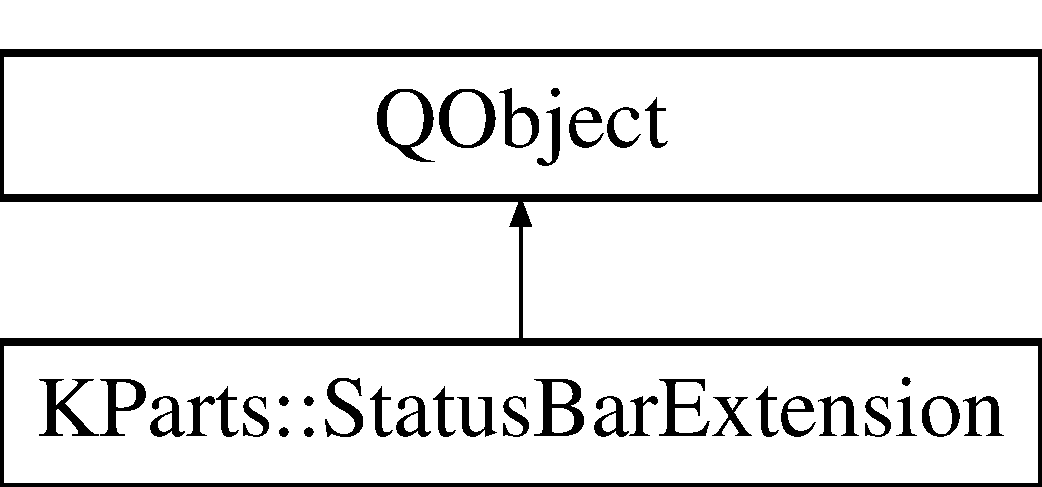
\includegraphics[height=2.000000cm]{classKParts_1_1StatusBarExtension}
\end{center}
\end{figure}
\subsection*{Public Member Functions}
\begin{DoxyCompactItemize}
\item 
\hyperlink{classKParts_1_1StatusBarExtension_a0130c3d5e970d44be6e1543cd5ae7324}{Status\+Bar\+Extension} (\hyperlink{classKParts_1_1ReadOnlyPart}{K\+Parts\+::\+Read\+Only\+Part} $\ast$parent)
\item 
\hyperlink{classKParts_1_1StatusBarExtension_a47bc9c8acae9b46bfa04ea0297e80bd8}{$\sim$\+Status\+Bar\+Extension} ()
\item 
void \hyperlink{classKParts_1_1StatusBarExtension_aaa7efe1d1a03b9d613c5bb8cbb6691d4}{add\+Status\+Bar\+Item} (Q\+Widget $\ast$widget, int stretch, bool permanent)
\item 
void \hyperlink{classKParts_1_1StatusBarExtension_adaef7e1acbb9373168ae531e0792ab6e}{remove\+Status\+Bar\+Item} (Q\+Widget $\ast$widget)
\item 
K\+Status\+Bar $\ast$ \hyperlink{classKParts_1_1StatusBarExtension_a561eaf86df9e40f4217d0cfed58d92bb}{status\+Bar} () const 
\item 
void \hyperlink{classKParts_1_1StatusBarExtension_a6e3e3e8969ec67285ef7749f6c9caa85}{set\+Status\+Bar} (K\+Status\+Bar $\ast$status)
\item 
virtual bool \hyperlink{classKParts_1_1StatusBarExtension_a05a310b221e20aa0ba60156be82a37ef}{event\+Filter} (Q\+Object $\ast$watched, Q\+Event $\ast$ev)
\end{DoxyCompactItemize}
\subsection*{Static Public Member Functions}
\begin{DoxyCompactItemize}
\item 
static \hyperlink{classKParts_1_1StatusBarExtension}{Status\+Bar\+Extension} $\ast$ \hyperlink{classKParts_1_1StatusBarExtension_a69c6c7a09941dd6c70b315a4c21f3f20}{child\+Object} (Q\+Object $\ast$obj)
\end{DoxyCompactItemize}
\subsection*{Friends}
\begin{DoxyCompactItemize}
\item 
class \hyperlink{classKParts_1_1StatusBarExtension_ad7fbe21a7ea073280f28211d53f7d775}{Status\+Bar\+Extension\+Private}
\end{DoxyCompactItemize}


\subsection{Detailed Description}
an extension for \hyperlink{namespaceKParts}{K\+Parts} that allows more sophisticated statusbar handling 

Every part can use this class to customize the statusbar as long as it is active. Add items via add\+Status\+Bar\+Item and remove an item with remove\+Status\+Bar\+Item.

I\+M\+P\+O\+R\+T\+A\+N\+T\+: do N\+O\+T add any items immediately after constructing the extension. Give the application time to set the statusbar in the extension if necessary. 

Definition at line 52 of file statusbarextension.\+h.



\subsection{Constructor \& Destructor Documentation}
\hypertarget{classKParts_1_1StatusBarExtension_a0130c3d5e970d44be6e1543cd5ae7324}{\index{K\+Parts\+::\+Status\+Bar\+Extension@{K\+Parts\+::\+Status\+Bar\+Extension}!Status\+Bar\+Extension@{Status\+Bar\+Extension}}
\index{Status\+Bar\+Extension@{Status\+Bar\+Extension}!K\+Parts\+::\+Status\+Bar\+Extension@{K\+Parts\+::\+Status\+Bar\+Extension}}
\subsubsection[{Status\+Bar\+Extension}]{\setlength{\rightskip}{0pt plus 5cm}K\+Parts\+::\+Status\+Bar\+Extension\+::\+Status\+Bar\+Extension (
\begin{DoxyParamCaption}
\item[{{\bf K\+Parts\+::\+Read\+Only\+Part} $\ast$}]{parent}
\end{DoxyParamCaption}
)}}\label{classKParts_1_1StatusBarExtension_a0130c3d5e970d44be6e1543cd5ae7324}
\hypertarget{classKParts_1_1StatusBarExtension_a47bc9c8acae9b46bfa04ea0297e80bd8}{\index{K\+Parts\+::\+Status\+Bar\+Extension@{K\+Parts\+::\+Status\+Bar\+Extension}!````~Status\+Bar\+Extension@{$\sim$\+Status\+Bar\+Extension}}
\index{````~Status\+Bar\+Extension@{$\sim$\+Status\+Bar\+Extension}!K\+Parts\+::\+Status\+Bar\+Extension@{K\+Parts\+::\+Status\+Bar\+Extension}}
\subsubsection[{$\sim$\+Status\+Bar\+Extension}]{\setlength{\rightskip}{0pt plus 5cm}K\+Parts\+::\+Status\+Bar\+Extension\+::$\sim$\+Status\+Bar\+Extension (
\begin{DoxyParamCaption}
{}
\end{DoxyParamCaption}
)}}\label{classKParts_1_1StatusBarExtension_a47bc9c8acae9b46bfa04ea0297e80bd8}


\subsection{Member Function Documentation}
\hypertarget{classKParts_1_1StatusBarExtension_aaa7efe1d1a03b9d613c5bb8cbb6691d4}{\index{K\+Parts\+::\+Status\+Bar\+Extension@{K\+Parts\+::\+Status\+Bar\+Extension}!add\+Status\+Bar\+Item@{add\+Status\+Bar\+Item}}
\index{add\+Status\+Bar\+Item@{add\+Status\+Bar\+Item}!K\+Parts\+::\+Status\+Bar\+Extension@{K\+Parts\+::\+Status\+Bar\+Extension}}
\subsubsection[{add\+Status\+Bar\+Item}]{\setlength{\rightskip}{0pt plus 5cm}void K\+Parts\+::\+Status\+Bar\+Extension\+::add\+Status\+Bar\+Item (
\begin{DoxyParamCaption}
\item[{Q\+Widget $\ast$}]{widget, }
\item[{int}]{stretch, }
\item[{bool}]{permanent}
\end{DoxyParamCaption}
)}}\label{classKParts_1_1StatusBarExtension_aaa7efe1d1a03b9d613c5bb8cbb6691d4}
This adds a widget to the statusbar for this part. If you use this method instead of using \hyperlink{classKParts_1_1StatusBarExtension_a561eaf86df9e40f4217d0cfed58d92bb}{status\+Bar()} directly, this extension will take care of removing the items when the parts G\+U\+I is deactivated and will re-\/add them when it is reactivated. The parameters are the same as Q\+Status\+Bar\+::add\+Widget().

Note that you can't use K\+Status\+Bar methods (inserting text items by id) but you can create a K\+Status\+Bar\+Label with a dummy id instead, and use it directly in order to get the same look and feel.


\begin{DoxyParams}{Parameters}
{\em widget} & the widget to add \\
\hline
{\em stretch} & the stretch factor. 0 for a minimum size. \\
\hline
{\em permanent} & passed to Q\+Status\+Bar\+::add\+Widget as the \char`\"{}permanent\char`\"{} bool. Note that the item isn't really permanent though, it goes away when the part is unactivated. This simply controls where temporary messages hide the {\ttfamily widget}, and whether it's added to the left or to the right side.\\
\hline
\end{DoxyParams}
that the widget does not technically become a child of the \hyperlink{classKParts_1_1StatusBarExtension}{Status\+Bar\+Extension} in a Q\+Object sense. However, it {\itshape will} be deleted when the \hyperlink{classKParts_1_1StatusBarExtension}{Status\+Bar\+Extension} is deleted.

I\+M\+P\+O\+R\+T\+A\+N\+T\+: do N\+O\+T add any items immediately after constructing the extension. Give the application time to set the statusbar in the extension if necessary. \hypertarget{classKParts_1_1StatusBarExtension_a69c6c7a09941dd6c70b315a4c21f3f20}{\index{K\+Parts\+::\+Status\+Bar\+Extension@{K\+Parts\+::\+Status\+Bar\+Extension}!child\+Object@{child\+Object}}
\index{child\+Object@{child\+Object}!K\+Parts\+::\+Status\+Bar\+Extension@{K\+Parts\+::\+Status\+Bar\+Extension}}
\subsubsection[{child\+Object}]{\setlength{\rightskip}{0pt plus 5cm}static {\bf Status\+Bar\+Extension}$\ast$ K\+Parts\+::\+Status\+Bar\+Extension\+::child\+Object (
\begin{DoxyParamCaption}
\item[{Q\+Object $\ast$}]{obj}
\end{DoxyParamCaption}
)\hspace{0.3cm}{\ttfamily [static]}}}\label{classKParts_1_1StatusBarExtension_a69c6c7a09941dd6c70b315a4c21f3f20}
Queries {\ttfamily obj} for a child object which inherits from this \hyperlink{classKParts_1_1BrowserExtension}{Browser\+Extension} class. Convenience method. \hypertarget{classKParts_1_1StatusBarExtension_a05a310b221e20aa0ba60156be82a37ef}{\index{K\+Parts\+::\+Status\+Bar\+Extension@{K\+Parts\+::\+Status\+Bar\+Extension}!event\+Filter@{event\+Filter}}
\index{event\+Filter@{event\+Filter}!K\+Parts\+::\+Status\+Bar\+Extension@{K\+Parts\+::\+Status\+Bar\+Extension}}
\subsubsection[{event\+Filter}]{\setlength{\rightskip}{0pt plus 5cm}virtual bool K\+Parts\+::\+Status\+Bar\+Extension\+::event\+Filter (
\begin{DoxyParamCaption}
\item[{Q\+Object $\ast$}]{watched, }
\item[{Q\+Event $\ast$}]{ev}
\end{DoxyParamCaption}
)\hspace{0.3cm}{\ttfamily [virtual]}}}\label{classKParts_1_1StatusBarExtension_a05a310b221e20aa0ba60156be82a37ef}
\hypertarget{classKParts_1_1StatusBarExtension_adaef7e1acbb9373168ae531e0792ab6e}{\index{K\+Parts\+::\+Status\+Bar\+Extension@{K\+Parts\+::\+Status\+Bar\+Extension}!remove\+Status\+Bar\+Item@{remove\+Status\+Bar\+Item}}
\index{remove\+Status\+Bar\+Item@{remove\+Status\+Bar\+Item}!K\+Parts\+::\+Status\+Bar\+Extension@{K\+Parts\+::\+Status\+Bar\+Extension}}
\subsubsection[{remove\+Status\+Bar\+Item}]{\setlength{\rightskip}{0pt plus 5cm}void K\+Parts\+::\+Status\+Bar\+Extension\+::remove\+Status\+Bar\+Item (
\begin{DoxyParamCaption}
\item[{Q\+Widget $\ast$}]{widget}
\end{DoxyParamCaption}
)}}\label{classKParts_1_1StatusBarExtension_adaef7e1acbb9373168ae531e0792ab6e}
Remove a widget from the statusbar for this part. \hypertarget{classKParts_1_1StatusBarExtension_a6e3e3e8969ec67285ef7749f6c9caa85}{\index{K\+Parts\+::\+Status\+Bar\+Extension@{K\+Parts\+::\+Status\+Bar\+Extension}!set\+Status\+Bar@{set\+Status\+Bar}}
\index{set\+Status\+Bar@{set\+Status\+Bar}!K\+Parts\+::\+Status\+Bar\+Extension@{K\+Parts\+::\+Status\+Bar\+Extension}}
\subsubsection[{set\+Status\+Bar}]{\setlength{\rightskip}{0pt plus 5cm}void K\+Parts\+::\+Status\+Bar\+Extension\+::set\+Status\+Bar (
\begin{DoxyParamCaption}
\item[{K\+Status\+Bar $\ast$}]{status}
\end{DoxyParamCaption}
)}}\label{classKParts_1_1StatusBarExtension_a6e3e3e8969ec67285ef7749f6c9caa85}
This allows the hosting application to set a particular K\+Status\+Bar for this part. If it doesn't do this, the statusbar used will be the one of the K\+Main\+Window in which the part is embedded. Konqueror uses this to assign a view-\/statusbar to the part. The part should never call this method! \hypertarget{classKParts_1_1StatusBarExtension_a561eaf86df9e40f4217d0cfed58d92bb}{\index{K\+Parts\+::\+Status\+Bar\+Extension@{K\+Parts\+::\+Status\+Bar\+Extension}!status\+Bar@{status\+Bar}}
\index{status\+Bar@{status\+Bar}!K\+Parts\+::\+Status\+Bar\+Extension@{K\+Parts\+::\+Status\+Bar\+Extension}}
\subsubsection[{status\+Bar}]{\setlength{\rightskip}{0pt plus 5cm}K\+Status\+Bar$\ast$ K\+Parts\+::\+Status\+Bar\+Extension\+::status\+Bar (
\begin{DoxyParamCaption}
{}
\end{DoxyParamCaption}
) const}}\label{classKParts_1_1StatusBarExtension_a561eaf86df9e40f4217d0cfed58d92bb}
\begin{DoxyReturn}{Returns}
the statusbar of the K\+Main\+Window in which this part is currently embedded. W\+A\+R\+N\+I\+N\+G\+: this could return 0\+L 
\end{DoxyReturn}


\subsection{Friends And Related Function Documentation}
\hypertarget{classKParts_1_1StatusBarExtension_ad7fbe21a7ea073280f28211d53f7d775}{\index{K\+Parts\+::\+Status\+Bar\+Extension@{K\+Parts\+::\+Status\+Bar\+Extension}!Status\+Bar\+Extension\+Private@{Status\+Bar\+Extension\+Private}}
\index{Status\+Bar\+Extension\+Private@{Status\+Bar\+Extension\+Private}!K\+Parts\+::\+Status\+Bar\+Extension@{K\+Parts\+::\+Status\+Bar\+Extension}}
\subsubsection[{Status\+Bar\+Extension\+Private}]{\setlength{\rightskip}{0pt plus 5cm}friend class Status\+Bar\+Extension\+Private\hspace{0.3cm}{\ttfamily [friend]}}}\label{classKParts_1_1StatusBarExtension_ad7fbe21a7ea073280f28211d53f7d775}


Definition at line 118 of file statusbarextension.\+h.



The documentation for this class was generated from the following file\+:\begin{DoxyCompactItemize}
\item 
/usr/include/kparts/\hyperlink{statusbarextension_8h}{statusbarextension.\+h}\end{DoxyCompactItemize}

\hypertarget{classKParts_1_1TextExtension}{\section{\-K\-Parts\-:\-:\-Text\-Extension \-Class \-Reference}
\label{classKParts_1_1TextExtension}\index{\-K\-Parts\-::\-Text\-Extension@{\-K\-Parts\-::\-Text\-Extension}}
}


an extension for \hyperlink{namespaceKParts}{\-K\-Parts} that allows to retrieve text from the part.  




{\ttfamily \#include $<$textextension.\-h$>$}

\subsection*{\-Public \-Types}
\begin{DoxyCompactItemize}
\item 
enum \hyperlink{classKParts_1_1TextExtension_a65ad08598c74eae19f0c7772a251685d}{\-Format} \{ \hyperlink{classKParts_1_1TextExtension_a65ad08598c74eae19f0c7772a251685da8bb1bd219fcb9237fae7b81b6d640f96}{\-Plain\-Text}, 
\hyperlink{classKParts_1_1TextExtension_a65ad08598c74eae19f0c7772a251685da330994e99d37a75f3720547767822f37}{\-H\-T\-M\-L}
 \}
\end{DoxyCompactItemize}
\subsection*{\-Signals}
\begin{DoxyCompactItemize}
\item 
void \hyperlink{classKParts_1_1TextExtension_a4d5e1cb28d1faa2dbccef3bb41c058f9}{selection\-Changed} ()
\end{DoxyCompactItemize}
\subsection*{\-Public \-Member \-Functions}
\begin{DoxyCompactItemize}
\item 
\hyperlink{classKParts_1_1TextExtension_a1c7077a3114c42f4b6cf78d4254fe5d0}{\-Text\-Extension} (\hyperlink{classKParts_1_1ReadOnlyPart}{\-K\-Parts\-::\-Read\-Only\-Part} $\ast$parent)
\item 
\hyperlink{classKParts_1_1TextExtension_a6d4e46c6cc819826182c3fc522a36b71}{$\sim$\-Text\-Extension} ()
\item 
virtual bool \hyperlink{classKParts_1_1TextExtension_a68623c6e7e7f57967c382550ccb3c00e}{has\-Selection} () const 
\item 
virtual \-Q\-String \hyperlink{classKParts_1_1TextExtension_a5ea4fb6f2237489affcde7c03e531574}{selected\-Text} (\hyperlink{classKParts_1_1TextExtension_a65ad08598c74eae19f0c7772a251685d}{\-Format} format) const 
\item 
virtual \-Q\-String \hyperlink{classKParts_1_1TextExtension_a42209cf90f31da5a3b01087518ad8625}{complete\-Text} (\hyperlink{classKParts_1_1TextExtension_a65ad08598c74eae19f0c7772a251685d}{\-Format} format) const 
\item 
virtual int \hyperlink{classKParts_1_1TextExtension_a62e0cd5df36c13591ed526bf58487d96}{page\-Count} () const 
\item 
virtual int \hyperlink{classKParts_1_1TextExtension_a3351795dd9a2257127ce978aaff68448}{current\-Page} () const 
\item 
virtual \-Q\-String \hyperlink{classKParts_1_1TextExtension_ab0a417697ec8edb599ba35f38bf90261}{page\-Text} (\hyperlink{classKParts_1_1TextExtension_a65ad08598c74eae19f0c7772a251685d}{\-Format} format) const 
\item 
virtual bool \hyperlink{classKParts_1_1TextExtension_aaaf29f56cbe212b3eea11d3811bfd270}{find\-Text} (const \-Q\-String \&string, \-K\-Find\-::\-Search\-Options options) const 
\end{DoxyCompactItemize}
\subsection*{\-Static \-Public \-Member \-Functions}
\begin{DoxyCompactItemize}
\item 
static \hyperlink{classKParts_1_1TextExtension}{\-Text\-Extension} $\ast$ \hyperlink{classKParts_1_1TextExtension_ae6a6df769ff322ad46396e83f26e8dec}{child\-Object} (\-Q\-Object $\ast$obj)
\end{DoxyCompactItemize}


\subsection{\-Detailed \-Description}
an extension for \hyperlink{namespaceKParts}{\-K\-Parts} that allows to retrieve text from the part. 

\-For instance, the text-\/to-\/speech plugin uses this to speak the whole text from the part or the selected text. \-The translation plugin uses it for translating the selected text, and so on.

\begin{DoxySince}{\-Since}
4.\-6 
\end{DoxySince}


\-Definition at line 42 of file textextension.\-h.



\subsection{\-Member \-Enumeration \-Documentation}
\hypertarget{classKParts_1_1TextExtension_a65ad08598c74eae19f0c7772a251685d}{\index{\-K\-Parts\-::\-Text\-Extension@{\-K\-Parts\-::\-Text\-Extension}!\-Format@{\-Format}}
\index{\-Format@{\-Format}!KParts::TextExtension@{\-K\-Parts\-::\-Text\-Extension}}
\subsubsection[{\-Format}]{\setlength{\rightskip}{0pt plus 5cm}enum {\bf \-K\-Parts\-::\-Text\-Extension\-::\-Format}}}\label{classKParts_1_1TextExtension_a65ad08598c74eae19f0c7772a251685d}
\begin{Desc}
\item[\-Enumerator\-: ]\par
\begin{description}
\index{\-Plain\-Text@{\-Plain\-Text}!\-K\-Parts\-::\-Text\-Extension@{\-K\-Parts\-::\-Text\-Extension}}\index{\-K\-Parts\-::\-Text\-Extension@{\-K\-Parts\-::\-Text\-Extension}!\-Plain\-Text@{\-Plain\-Text}}\item[{\em 
\hypertarget{classKParts_1_1TextExtension_a65ad08598c74eae19f0c7772a251685da8bb1bd219fcb9237fae7b81b6d640f96}{\-Plain\-Text}\label{classKParts_1_1TextExtension_a65ad08598c74eae19f0c7772a251685da8bb1bd219fcb9237fae7b81b6d640f96}
}]\index{\-H\-T\-M\-L@{\-H\-T\-M\-L}!\-K\-Parts\-::\-Text\-Extension@{\-K\-Parts\-::\-Text\-Extension}}\index{\-K\-Parts\-::\-Text\-Extension@{\-K\-Parts\-::\-Text\-Extension}!\-H\-T\-M\-L@{\-H\-T\-M\-L}}\item[{\em 
\hypertarget{classKParts_1_1TextExtension_a65ad08598c74eae19f0c7772a251685da330994e99d37a75f3720547767822f37}{\-H\-T\-M\-L}\label{classKParts_1_1TextExtension_a65ad08598c74eae19f0c7772a251685da330994e99d37a75f3720547767822f37}
}]\end{description}
\end{Desc}



\-Definition at line 55 of file textextension.\-h.


\begin{DoxyCode}
{ PlainText, HTML };
\end{DoxyCode}


\subsection{\-Constructor \& \-Destructor \-Documentation}
\hypertarget{classKParts_1_1TextExtension_a1c7077a3114c42f4b6cf78d4254fe5d0}{\index{\-K\-Parts\-::\-Text\-Extension@{\-K\-Parts\-::\-Text\-Extension}!\-Text\-Extension@{\-Text\-Extension}}
\index{\-Text\-Extension@{\-Text\-Extension}!KParts::TextExtension@{\-K\-Parts\-::\-Text\-Extension}}
\subsubsection[{\-Text\-Extension}]{\setlength{\rightskip}{0pt plus 5cm}{\bf \-K\-Parts\-::\-Text\-Extension\-::\-Text\-Extension} (
\begin{DoxyParamCaption}
\item[{{\bf \-K\-Parts\-::\-Read\-Only\-Part} $\ast$}]{parent}
\end{DoxyParamCaption}
)}}\label{classKParts_1_1TextExtension_a1c7077a3114c42f4b6cf78d4254fe5d0}
\hypertarget{classKParts_1_1TextExtension_a6d4e46c6cc819826182c3fc522a36b71}{\index{\-K\-Parts\-::\-Text\-Extension@{\-K\-Parts\-::\-Text\-Extension}!$\sim$\-Text\-Extension@{$\sim$\-Text\-Extension}}
\index{$\sim$\-Text\-Extension@{$\sim$\-Text\-Extension}!KParts::TextExtension@{\-K\-Parts\-::\-Text\-Extension}}
\subsubsection[{$\sim$\-Text\-Extension}]{\setlength{\rightskip}{0pt plus 5cm}{\bf \-K\-Parts\-::\-Text\-Extension\-::$\sim$\-Text\-Extension} (
\begin{DoxyParamCaption}
{}
\end{DoxyParamCaption}
)}}\label{classKParts_1_1TextExtension_a6d4e46c6cc819826182c3fc522a36b71}


\subsection{\-Member \-Function \-Documentation}
\hypertarget{classKParts_1_1TextExtension_ae6a6df769ff322ad46396e83f26e8dec}{\index{\-K\-Parts\-::\-Text\-Extension@{\-K\-Parts\-::\-Text\-Extension}!child\-Object@{child\-Object}}
\index{child\-Object@{child\-Object}!KParts::TextExtension@{\-K\-Parts\-::\-Text\-Extension}}
\subsubsection[{child\-Object}]{\setlength{\rightskip}{0pt plus 5cm}static {\bf \-Text\-Extension}$\ast$ {\bf \-K\-Parts\-::\-Text\-Extension\-::child\-Object} (
\begin{DoxyParamCaption}
\item[{\-Q\-Object $\ast$}]{obj}
\end{DoxyParamCaption}
)\hspace{0.3cm}{\ttfamily  \mbox{[}static\mbox{]}}}}\label{classKParts_1_1TextExtension_ae6a6df769ff322ad46396e83f26e8dec}
\-Queries {\ttfamily obj} for a child object which inherits from this \hyperlink{classKParts_1_1TextExtension}{\-Text\-Extension} class. \hypertarget{classKParts_1_1TextExtension_a42209cf90f31da5a3b01087518ad8625}{\index{\-K\-Parts\-::\-Text\-Extension@{\-K\-Parts\-::\-Text\-Extension}!complete\-Text@{complete\-Text}}
\index{complete\-Text@{complete\-Text}!KParts::TextExtension@{\-K\-Parts\-::\-Text\-Extension}}
\subsubsection[{complete\-Text}]{\setlength{\rightskip}{0pt plus 5cm}virtual \-Q\-String {\bf \-K\-Parts\-::\-Text\-Extension\-::complete\-Text} (
\begin{DoxyParamCaption}
\item[{{\bf \-Format}}]{format}
\end{DoxyParamCaption}
) const\hspace{0.3cm}{\ttfamily  \mbox{[}virtual\mbox{]}}}}\label{classKParts_1_1TextExtension_a42209cf90f31da5a3b01087518ad8625}
\-Returns the complete text shown in the part, in the requested format. \-If the format is not supported, the part must return an empty string. \hypertarget{classKParts_1_1TextExtension_a3351795dd9a2257127ce978aaff68448}{\index{\-K\-Parts\-::\-Text\-Extension@{\-K\-Parts\-::\-Text\-Extension}!current\-Page@{current\-Page}}
\index{current\-Page@{current\-Page}!KParts::TextExtension@{\-K\-Parts\-::\-Text\-Extension}}
\subsubsection[{current\-Page}]{\setlength{\rightskip}{0pt plus 5cm}virtual int {\bf \-K\-Parts\-::\-Text\-Extension\-::current\-Page} (
\begin{DoxyParamCaption}
{}
\end{DoxyParamCaption}
) const\hspace{0.3cm}{\ttfamily  \mbox{[}virtual\mbox{]}}}}\label{classKParts_1_1TextExtension_a3351795dd9a2257127ce978aaff68448}
\-Returns the current page (between 0 and \hyperlink{classKParts_1_1TextExtension_a62e0cd5df36c13591ed526bf58487d96}{page\-Count()}-\/1), for parts who support the concept of pages. \-Otherwise returns 0. \hypertarget{classKParts_1_1TextExtension_aaaf29f56cbe212b3eea11d3811bfd270}{\index{\-K\-Parts\-::\-Text\-Extension@{\-K\-Parts\-::\-Text\-Extension}!find\-Text@{find\-Text}}
\index{find\-Text@{find\-Text}!KParts::TextExtension@{\-K\-Parts\-::\-Text\-Extension}}
\subsubsection[{find\-Text}]{\setlength{\rightskip}{0pt plus 5cm}virtual bool {\bf \-K\-Parts\-::\-Text\-Extension\-::find\-Text} (
\begin{DoxyParamCaption}
\item[{const \-Q\-String \&}]{string, }
\item[{\-K\-Find\-::\-Search\-Options}]{options}
\end{DoxyParamCaption}
) const\hspace{0.3cm}{\ttfamily  \mbox{[}virtual\mbox{]}}}}\label{classKParts_1_1TextExtension_aaaf29f56cbe212b3eea11d3811bfd270}
\-Returns true if {\ttfamily string} is found using the given {\ttfamily options}.

\-If any text matches {\ttfamily string}, then it will be selected/highlighted. \-To find the next matching text, simply call this function again with the same search text until it returns false.

\-To clear a selection, just pass an empty string.

\-Note that parts that implement this extension might not support all the options available in \-K\-Find\-::\-Search\-Options. \hypertarget{classKParts_1_1TextExtension_a68623c6e7e7f57967c382550ccb3c00e}{\index{\-K\-Parts\-::\-Text\-Extension@{\-K\-Parts\-::\-Text\-Extension}!has\-Selection@{has\-Selection}}
\index{has\-Selection@{has\-Selection}!KParts::TextExtension@{\-K\-Parts\-::\-Text\-Extension}}
\subsubsection[{has\-Selection}]{\setlength{\rightskip}{0pt plus 5cm}virtual bool {\bf \-K\-Parts\-::\-Text\-Extension\-::has\-Selection} (
\begin{DoxyParamCaption}
{}
\end{DoxyParamCaption}
) const\hspace{0.3cm}{\ttfamily  \mbox{[}virtual\mbox{]}}}}\label{classKParts_1_1TextExtension_a68623c6e7e7f57967c382550ccb3c00e}
\-Returns true if the user selected text in the part. \hypertarget{classKParts_1_1TextExtension_a62e0cd5df36c13591ed526bf58487d96}{\index{\-K\-Parts\-::\-Text\-Extension@{\-K\-Parts\-::\-Text\-Extension}!page\-Count@{page\-Count}}
\index{page\-Count@{page\-Count}!KParts::TextExtension@{\-K\-Parts\-::\-Text\-Extension}}
\subsubsection[{page\-Count}]{\setlength{\rightskip}{0pt plus 5cm}virtual int {\bf \-K\-Parts\-::\-Text\-Extension\-::page\-Count} (
\begin{DoxyParamCaption}
{}
\end{DoxyParamCaption}
) const\hspace{0.3cm}{\ttfamily  \mbox{[}virtual\mbox{]}}}}\label{classKParts_1_1TextExtension_a62e0cd5df36c13591ed526bf58487d96}
\-Returns the number of pages, for parts who support the concept of pages. \-Otherwise returns 0. \hypertarget{classKParts_1_1TextExtension_ab0a417697ec8edb599ba35f38bf90261}{\index{\-K\-Parts\-::\-Text\-Extension@{\-K\-Parts\-::\-Text\-Extension}!page\-Text@{page\-Text}}
\index{page\-Text@{page\-Text}!KParts::TextExtension@{\-K\-Parts\-::\-Text\-Extension}}
\subsubsection[{page\-Text}]{\setlength{\rightskip}{0pt plus 5cm}virtual \-Q\-String {\bf \-K\-Parts\-::\-Text\-Extension\-::page\-Text} (
\begin{DoxyParamCaption}
\item[{{\bf \-Format}}]{format}
\end{DoxyParamCaption}
) const\hspace{0.3cm}{\ttfamily  \mbox{[}virtual\mbox{]}}}}\label{classKParts_1_1TextExtension_ab0a417697ec8edb599ba35f38bf90261}
\-Returns the text in a given page, in the requested format. \hypertarget{classKParts_1_1TextExtension_a5ea4fb6f2237489affcde7c03e531574}{\index{\-K\-Parts\-::\-Text\-Extension@{\-K\-Parts\-::\-Text\-Extension}!selected\-Text@{selected\-Text}}
\index{selected\-Text@{selected\-Text}!KParts::TextExtension@{\-K\-Parts\-::\-Text\-Extension}}
\subsubsection[{selected\-Text}]{\setlength{\rightskip}{0pt plus 5cm}virtual \-Q\-String {\bf \-K\-Parts\-::\-Text\-Extension\-::selected\-Text} (
\begin{DoxyParamCaption}
\item[{{\bf \-Format}}]{format}
\end{DoxyParamCaption}
) const\hspace{0.3cm}{\ttfamily  \mbox{[}virtual\mbox{]}}}}\label{classKParts_1_1TextExtension_a5ea4fb6f2237489affcde7c03e531574}
\-Returns the selected text, in the requested format. \-If the format is not supported, the part must return an empty string. \hypertarget{classKParts_1_1TextExtension_a4d5e1cb28d1faa2dbccef3bb41c058f9}{\index{\-K\-Parts\-::\-Text\-Extension@{\-K\-Parts\-::\-Text\-Extension}!selection\-Changed@{selection\-Changed}}
\index{selection\-Changed@{selection\-Changed}!KParts::TextExtension@{\-K\-Parts\-::\-Text\-Extension}}
\subsubsection[{selection\-Changed}]{\setlength{\rightskip}{0pt plus 5cm}void {\bf \-K\-Parts\-::\-Text\-Extension\-::selection\-Changed} (
\begin{DoxyParamCaption}
{}
\end{DoxyParamCaption}
)\hspace{0.3cm}{\ttfamily  \mbox{[}signal\mbox{]}}}}\label{classKParts_1_1TextExtension_a4d5e1cb28d1faa2dbccef3bb41c058f9}
\-This signal is emitted when the selection changes. 

\-The documentation for this class was generated from the following file\-:\begin{DoxyCompactItemize}
\item 
/usr/include/kparts/\hyperlink{textextension_8h}{textextension.\-h}\end{DoxyCompactItemize}

\hypertarget{structKParts_1_1ScriptableExtension_1_1Undefined}{\section{\-K\-Parts\-:\-:\-Scriptable\-Extension\-:\-:\-Undefined \-Struct \-Reference}
\label{structKParts_1_1ScriptableExtension_1_1Undefined}\index{\-K\-Parts\-::\-Scriptable\-Extension\-::\-Undefined@{\-K\-Parts\-::\-Scriptable\-Extension\-::\-Undefined}}
}


\-Corresponds to 'undefined' in \-Java\-Script.  




{\ttfamily \#include $<$scriptableextension.\-h$>$}



\subsection{\-Detailed \-Description}
\-Corresponds to 'undefined' in \-Java\-Script. 

\-Definition at line 64 of file scriptableextension.\-h.



\-The documentation for this struct was generated from the following file\-:\begin{DoxyCompactItemize}
\item 
/usr/include/kparts/\hyperlink{scriptableextension_8h}{scriptableextension.\-h}\end{DoxyCompactItemize}

\hypertarget{classKParts_1_1WindowArgs}{\section{K\+Parts\+:\+:Window\+Args Class Reference}
\label{classKParts_1_1WindowArgs}\index{K\+Parts\+::\+Window\+Args@{K\+Parts\+::\+Window\+Args}}
}


{\ttfamily \#include $<$browserextension.\+h$>$}

\subsection*{Public Member Functions}
\begin{DoxyCompactItemize}
\item 
\hyperlink{classKParts_1_1WindowArgs_a6ba69542d139ad2d0028217e5ddb3e29}{Window\+Args} ()
\item 
\hyperlink{classKParts_1_1WindowArgs_a3055e556ecc5e135b6e9c79e2d389030}{$\sim$\+Window\+Args} ()
\item 
\hyperlink{classKParts_1_1WindowArgs_a2d5689aada5007fecb06ab424b9e7e29}{Window\+Args} (const \hyperlink{classKParts_1_1WindowArgs}{Window\+Args} \&args)
\item 
\hyperlink{classKParts_1_1WindowArgs}{Window\+Args} \& \hyperlink{classKParts_1_1WindowArgs_ab066d5b00f6d530333741ff962dc7a98}{operator=} (const \hyperlink{classKParts_1_1WindowArgs}{Window\+Args} \&args)
\item 
\hyperlink{classKParts_1_1WindowArgs_a5246d7180dfb422bbae2b0fa42cb7dae}{Window\+Args} (const Q\+Rect \&\+\_\+geometry, bool \+\_\+fullscreen, bool \+\_\+menu\+Bar\+Visible, bool \+\_\+tool\+Bars\+Visible, bool \+\_\+status\+Bar\+Visible, bool \+\_\+resizable)
\item 
\hyperlink{classKParts_1_1WindowArgs_a9a571192e827587dd0592260da03736e}{Window\+Args} (int \+\_\+x, int \+\_\+y, int \+\_\+width, int \+\_\+height, bool \+\_\+fullscreen, bool \+\_\+menu\+Bar\+Visible, bool \+\_\+tool\+Bars\+Visible, bool \+\_\+status\+Bar\+Visible, bool \+\_\+resizable)
\item 
void \hyperlink{classKParts_1_1WindowArgs_a6e2e25bf31a3778e80ad211f10cad269}{set\+X} (int \hyperlink{classKParts_1_1WindowArgs_a671ecb605228581b1b719a9407f4c2be}{x})
\item 
int \hyperlink{classKParts_1_1WindowArgs_a671ecb605228581b1b719a9407f4c2be}{x} () const 
\item 
void \hyperlink{classKParts_1_1WindowArgs_ae3f3e65be412324da1598110ec3273c9}{set\+Y} (int \hyperlink{classKParts_1_1WindowArgs_a3fcb463bb6b6e87fd9cd9fdd55ecd30b}{y})
\item 
int \hyperlink{classKParts_1_1WindowArgs_a3fcb463bb6b6e87fd9cd9fdd55ecd30b}{y} () const 
\item 
void \hyperlink{classKParts_1_1WindowArgs_a4af288c9b6ace9560aa5fc1e5af39de3}{set\+Width} (int w)
\item 
int \hyperlink{classKParts_1_1WindowArgs_a2e71e88878e5ed699cdc591715eee509}{width} () const 
\item 
void \hyperlink{classKParts_1_1WindowArgs_a85a07a9fafa90d79edfd338ad2a9dae5}{set\+Height} (int h)
\item 
int \hyperlink{classKParts_1_1WindowArgs_abc7756c372df99be8d83bc6e1574734a}{height} () const 
\item 
void \hyperlink{classKParts_1_1WindowArgs_a9779524444f507933ea314f5e31c893e}{set\+Full\+Screen} (bool fs)
\item 
bool \hyperlink{classKParts_1_1WindowArgs_a5bd1ed448fedb091f633c82104abdf97}{is\+Full\+Screen} () const 
\item 
void \hyperlink{classKParts_1_1WindowArgs_a8ea1f1f5a6fbc6f8db6b1564fb36926c}{set\+Menu\+Bar\+Visible} (bool visible)
\item 
bool \hyperlink{classKParts_1_1WindowArgs_abf3d15dc8f4267d1e3ad8e2bcb846283}{is\+Menu\+Bar\+Visible} () const 
\item 
void \hyperlink{classKParts_1_1WindowArgs_a14a892eb0edb68e49056e751bebf6425}{set\+Tool\+Bars\+Visible} (bool visible)
\item 
bool \hyperlink{classKParts_1_1WindowArgs_ac87b860b3157db4f6c5d1d512b3cfb8c}{tool\+Bars\+Visible} () const 
\item 
void \hyperlink{classKParts_1_1WindowArgs_acde0aa5cbc892404c4c3a8bfd9829eba}{set\+Status\+Bar\+Visible} (bool visible)
\item 
bool \hyperlink{classKParts_1_1WindowArgs_af2932404a1a223126e60e31737c62e11}{is\+Status\+Bar\+Visible} () const 
\item 
void \hyperlink{classKParts_1_1WindowArgs_a238f7aa7f8aebea2180d7b7cafa961c4}{set\+Resizable} (bool resizable)
\item 
bool \hyperlink{classKParts_1_1WindowArgs_a8031d2745585e35410e834ed5e7f1265}{is\+Resizable} () const 
\item 
void \hyperlink{classKParts_1_1WindowArgs_adebf8b4fb811f068cba27e6e2a050f0b}{set\+Lower\+Window} (bool lower)
\item 
bool \hyperlink{classKParts_1_1WindowArgs_a437e2bf77cfcd30b1d98b6160a4f4f2d}{lower\+Window} () const 
\item 
void \hyperlink{classKParts_1_1WindowArgs_a3f861f5f5ed4719e9c3d4ee8a688d18a}{set\+Scroll\+Bars\+Visible} (bool visible)
\item 
bool \hyperlink{classKParts_1_1WindowArgs_a9eb6ebe54b896f33f84d1379c71be18a}{scroll\+Bars\+Visible} () const 
\end{DoxyCompactItemize}


\subsection{Detailed Description}
The \hyperlink{classKParts_1_1WindowArgs}{Window\+Args} are used to specify arguments to the \char`\"{}create new window\char`\"{} call (see the create\+New\+Window variant that uses \hyperlink{classKParts_1_1WindowArgs}{Window\+Args}). The primary reason for this is the javascript window.\+open function. 

Definition at line 192 of file browserextension.\+h.



\subsection{Constructor \& Destructor Documentation}
\hypertarget{classKParts_1_1WindowArgs_a6ba69542d139ad2d0028217e5ddb3e29}{\index{K\+Parts\+::\+Window\+Args@{K\+Parts\+::\+Window\+Args}!Window\+Args@{Window\+Args}}
\index{Window\+Args@{Window\+Args}!K\+Parts\+::\+Window\+Args@{K\+Parts\+::\+Window\+Args}}
\subsubsection[{Window\+Args}]{\setlength{\rightskip}{0pt plus 5cm}K\+Parts\+::\+Window\+Args\+::\+Window\+Args (
\begin{DoxyParamCaption}
{}
\end{DoxyParamCaption}
)}}\label{classKParts_1_1WindowArgs_a6ba69542d139ad2d0028217e5ddb3e29}
\hypertarget{classKParts_1_1WindowArgs_a3055e556ecc5e135b6e9c79e2d389030}{\index{K\+Parts\+::\+Window\+Args@{K\+Parts\+::\+Window\+Args}!````~Window\+Args@{$\sim$\+Window\+Args}}
\index{````~Window\+Args@{$\sim$\+Window\+Args}!K\+Parts\+::\+Window\+Args@{K\+Parts\+::\+Window\+Args}}
\subsubsection[{$\sim$\+Window\+Args}]{\setlength{\rightskip}{0pt plus 5cm}K\+Parts\+::\+Window\+Args\+::$\sim$\+Window\+Args (
\begin{DoxyParamCaption}
{}
\end{DoxyParamCaption}
)}}\label{classKParts_1_1WindowArgs_a3055e556ecc5e135b6e9c79e2d389030}
\hypertarget{classKParts_1_1WindowArgs_a2d5689aada5007fecb06ab424b9e7e29}{\index{K\+Parts\+::\+Window\+Args@{K\+Parts\+::\+Window\+Args}!Window\+Args@{Window\+Args}}
\index{Window\+Args@{Window\+Args}!K\+Parts\+::\+Window\+Args@{K\+Parts\+::\+Window\+Args}}
\subsubsection[{Window\+Args}]{\setlength{\rightskip}{0pt plus 5cm}K\+Parts\+::\+Window\+Args\+::\+Window\+Args (
\begin{DoxyParamCaption}
\item[{const {\bf Window\+Args} \&}]{args}
\end{DoxyParamCaption}
)}}\label{classKParts_1_1WindowArgs_a2d5689aada5007fecb06ab424b9e7e29}
\hypertarget{classKParts_1_1WindowArgs_a5246d7180dfb422bbae2b0fa42cb7dae}{\index{K\+Parts\+::\+Window\+Args@{K\+Parts\+::\+Window\+Args}!Window\+Args@{Window\+Args}}
\index{Window\+Args@{Window\+Args}!K\+Parts\+::\+Window\+Args@{K\+Parts\+::\+Window\+Args}}
\subsubsection[{Window\+Args}]{\setlength{\rightskip}{0pt plus 5cm}K\+Parts\+::\+Window\+Args\+::\+Window\+Args (
\begin{DoxyParamCaption}
\item[{const Q\+Rect \&}]{\+\_\+geometry, }
\item[{bool}]{\+\_\+fullscreen, }
\item[{bool}]{\+\_\+menu\+Bar\+Visible, }
\item[{bool}]{\+\_\+tool\+Bars\+Visible, }
\item[{bool}]{\+\_\+status\+Bar\+Visible, }
\item[{bool}]{\+\_\+resizable}
\end{DoxyParamCaption}
)}}\label{classKParts_1_1WindowArgs_a5246d7180dfb422bbae2b0fa42cb7dae}
\hypertarget{classKParts_1_1WindowArgs_a9a571192e827587dd0592260da03736e}{\index{K\+Parts\+::\+Window\+Args@{K\+Parts\+::\+Window\+Args}!Window\+Args@{Window\+Args}}
\index{Window\+Args@{Window\+Args}!K\+Parts\+::\+Window\+Args@{K\+Parts\+::\+Window\+Args}}
\subsubsection[{Window\+Args}]{\setlength{\rightskip}{0pt plus 5cm}K\+Parts\+::\+Window\+Args\+::\+Window\+Args (
\begin{DoxyParamCaption}
\item[{int}]{\+\_\+x, }
\item[{int}]{\+\_\+y, }
\item[{int}]{\+\_\+width, }
\item[{int}]{\+\_\+height, }
\item[{bool}]{\+\_\+fullscreen, }
\item[{bool}]{\+\_\+menu\+Bar\+Visible, }
\item[{bool}]{\+\_\+tool\+Bars\+Visible, }
\item[{bool}]{\+\_\+status\+Bar\+Visible, }
\item[{bool}]{\+\_\+resizable}
\end{DoxyParamCaption}
)}}\label{classKParts_1_1WindowArgs_a9a571192e827587dd0592260da03736e}


\subsection{Member Function Documentation}
\hypertarget{classKParts_1_1WindowArgs_abc7756c372df99be8d83bc6e1574734a}{\index{K\+Parts\+::\+Window\+Args@{K\+Parts\+::\+Window\+Args}!height@{height}}
\index{height@{height}!K\+Parts\+::\+Window\+Args@{K\+Parts\+::\+Window\+Args}}
\subsubsection[{height}]{\setlength{\rightskip}{0pt plus 5cm}int K\+Parts\+::\+Window\+Args\+::height (
\begin{DoxyParamCaption}
{}
\end{DoxyParamCaption}
) const}}\label{classKParts_1_1WindowArgs_abc7756c372df99be8d83bc6e1574734a}
\hypertarget{classKParts_1_1WindowArgs_a5bd1ed448fedb091f633c82104abdf97}{\index{K\+Parts\+::\+Window\+Args@{K\+Parts\+::\+Window\+Args}!is\+Full\+Screen@{is\+Full\+Screen}}
\index{is\+Full\+Screen@{is\+Full\+Screen}!K\+Parts\+::\+Window\+Args@{K\+Parts\+::\+Window\+Args}}
\subsubsection[{is\+Full\+Screen}]{\setlength{\rightskip}{0pt plus 5cm}bool K\+Parts\+::\+Window\+Args\+::is\+Full\+Screen (
\begin{DoxyParamCaption}
{}
\end{DoxyParamCaption}
) const}}\label{classKParts_1_1WindowArgs_a5bd1ed448fedb091f633c82104abdf97}
\hypertarget{classKParts_1_1WindowArgs_abf3d15dc8f4267d1e3ad8e2bcb846283}{\index{K\+Parts\+::\+Window\+Args@{K\+Parts\+::\+Window\+Args}!is\+Menu\+Bar\+Visible@{is\+Menu\+Bar\+Visible}}
\index{is\+Menu\+Bar\+Visible@{is\+Menu\+Bar\+Visible}!K\+Parts\+::\+Window\+Args@{K\+Parts\+::\+Window\+Args}}
\subsubsection[{is\+Menu\+Bar\+Visible}]{\setlength{\rightskip}{0pt plus 5cm}bool K\+Parts\+::\+Window\+Args\+::is\+Menu\+Bar\+Visible (
\begin{DoxyParamCaption}
{}
\end{DoxyParamCaption}
) const}}\label{classKParts_1_1WindowArgs_abf3d15dc8f4267d1e3ad8e2bcb846283}
\hypertarget{classKParts_1_1WindowArgs_a8031d2745585e35410e834ed5e7f1265}{\index{K\+Parts\+::\+Window\+Args@{K\+Parts\+::\+Window\+Args}!is\+Resizable@{is\+Resizable}}
\index{is\+Resizable@{is\+Resizable}!K\+Parts\+::\+Window\+Args@{K\+Parts\+::\+Window\+Args}}
\subsubsection[{is\+Resizable}]{\setlength{\rightskip}{0pt plus 5cm}bool K\+Parts\+::\+Window\+Args\+::is\+Resizable (
\begin{DoxyParamCaption}
{}
\end{DoxyParamCaption}
) const}}\label{classKParts_1_1WindowArgs_a8031d2745585e35410e834ed5e7f1265}
\hypertarget{classKParts_1_1WindowArgs_af2932404a1a223126e60e31737c62e11}{\index{K\+Parts\+::\+Window\+Args@{K\+Parts\+::\+Window\+Args}!is\+Status\+Bar\+Visible@{is\+Status\+Bar\+Visible}}
\index{is\+Status\+Bar\+Visible@{is\+Status\+Bar\+Visible}!K\+Parts\+::\+Window\+Args@{K\+Parts\+::\+Window\+Args}}
\subsubsection[{is\+Status\+Bar\+Visible}]{\setlength{\rightskip}{0pt plus 5cm}bool K\+Parts\+::\+Window\+Args\+::is\+Status\+Bar\+Visible (
\begin{DoxyParamCaption}
{}
\end{DoxyParamCaption}
) const}}\label{classKParts_1_1WindowArgs_af2932404a1a223126e60e31737c62e11}
\hypertarget{classKParts_1_1WindowArgs_a437e2bf77cfcd30b1d98b6160a4f4f2d}{\index{K\+Parts\+::\+Window\+Args@{K\+Parts\+::\+Window\+Args}!lower\+Window@{lower\+Window}}
\index{lower\+Window@{lower\+Window}!K\+Parts\+::\+Window\+Args@{K\+Parts\+::\+Window\+Args}}
\subsubsection[{lower\+Window}]{\setlength{\rightskip}{0pt plus 5cm}bool K\+Parts\+::\+Window\+Args\+::lower\+Window (
\begin{DoxyParamCaption}
{}
\end{DoxyParamCaption}
) const}}\label{classKParts_1_1WindowArgs_a437e2bf77cfcd30b1d98b6160a4f4f2d}
\hypertarget{classKParts_1_1WindowArgs_ab066d5b00f6d530333741ff962dc7a98}{\index{K\+Parts\+::\+Window\+Args@{K\+Parts\+::\+Window\+Args}!operator=@{operator=}}
\index{operator=@{operator=}!K\+Parts\+::\+Window\+Args@{K\+Parts\+::\+Window\+Args}}
\subsubsection[{operator=}]{\setlength{\rightskip}{0pt plus 5cm}{\bf Window\+Args}\& K\+Parts\+::\+Window\+Args\+::operator= (
\begin{DoxyParamCaption}
\item[{const {\bf Window\+Args} \&}]{args}
\end{DoxyParamCaption}
)}}\label{classKParts_1_1WindowArgs_ab066d5b00f6d530333741ff962dc7a98}
\hypertarget{classKParts_1_1WindowArgs_a9eb6ebe54b896f33f84d1379c71be18a}{\index{K\+Parts\+::\+Window\+Args@{K\+Parts\+::\+Window\+Args}!scroll\+Bars\+Visible@{scroll\+Bars\+Visible}}
\index{scroll\+Bars\+Visible@{scroll\+Bars\+Visible}!K\+Parts\+::\+Window\+Args@{K\+Parts\+::\+Window\+Args}}
\subsubsection[{scroll\+Bars\+Visible}]{\setlength{\rightskip}{0pt plus 5cm}bool K\+Parts\+::\+Window\+Args\+::scroll\+Bars\+Visible (
\begin{DoxyParamCaption}
{}
\end{DoxyParamCaption}
) const}}\label{classKParts_1_1WindowArgs_a9eb6ebe54b896f33f84d1379c71be18a}
\hypertarget{classKParts_1_1WindowArgs_a9779524444f507933ea314f5e31c893e}{\index{K\+Parts\+::\+Window\+Args@{K\+Parts\+::\+Window\+Args}!set\+Full\+Screen@{set\+Full\+Screen}}
\index{set\+Full\+Screen@{set\+Full\+Screen}!K\+Parts\+::\+Window\+Args@{K\+Parts\+::\+Window\+Args}}
\subsubsection[{set\+Full\+Screen}]{\setlength{\rightskip}{0pt plus 5cm}void K\+Parts\+::\+Window\+Args\+::set\+Full\+Screen (
\begin{DoxyParamCaption}
\item[{bool}]{fs}
\end{DoxyParamCaption}
)}}\label{classKParts_1_1WindowArgs_a9779524444f507933ea314f5e31c893e}
\hypertarget{classKParts_1_1WindowArgs_a85a07a9fafa90d79edfd338ad2a9dae5}{\index{K\+Parts\+::\+Window\+Args@{K\+Parts\+::\+Window\+Args}!set\+Height@{set\+Height}}
\index{set\+Height@{set\+Height}!K\+Parts\+::\+Window\+Args@{K\+Parts\+::\+Window\+Args}}
\subsubsection[{set\+Height}]{\setlength{\rightskip}{0pt plus 5cm}void K\+Parts\+::\+Window\+Args\+::set\+Height (
\begin{DoxyParamCaption}
\item[{int}]{h}
\end{DoxyParamCaption}
)}}\label{classKParts_1_1WindowArgs_a85a07a9fafa90d79edfd338ad2a9dae5}
\hypertarget{classKParts_1_1WindowArgs_adebf8b4fb811f068cba27e6e2a050f0b}{\index{K\+Parts\+::\+Window\+Args@{K\+Parts\+::\+Window\+Args}!set\+Lower\+Window@{set\+Lower\+Window}}
\index{set\+Lower\+Window@{set\+Lower\+Window}!K\+Parts\+::\+Window\+Args@{K\+Parts\+::\+Window\+Args}}
\subsubsection[{set\+Lower\+Window}]{\setlength{\rightskip}{0pt plus 5cm}void K\+Parts\+::\+Window\+Args\+::set\+Lower\+Window (
\begin{DoxyParamCaption}
\item[{bool}]{lower}
\end{DoxyParamCaption}
)}}\label{classKParts_1_1WindowArgs_adebf8b4fb811f068cba27e6e2a050f0b}
\hypertarget{classKParts_1_1WindowArgs_a8ea1f1f5a6fbc6f8db6b1564fb36926c}{\index{K\+Parts\+::\+Window\+Args@{K\+Parts\+::\+Window\+Args}!set\+Menu\+Bar\+Visible@{set\+Menu\+Bar\+Visible}}
\index{set\+Menu\+Bar\+Visible@{set\+Menu\+Bar\+Visible}!K\+Parts\+::\+Window\+Args@{K\+Parts\+::\+Window\+Args}}
\subsubsection[{set\+Menu\+Bar\+Visible}]{\setlength{\rightskip}{0pt plus 5cm}void K\+Parts\+::\+Window\+Args\+::set\+Menu\+Bar\+Visible (
\begin{DoxyParamCaption}
\item[{bool}]{visible}
\end{DoxyParamCaption}
)}}\label{classKParts_1_1WindowArgs_a8ea1f1f5a6fbc6f8db6b1564fb36926c}
\hypertarget{classKParts_1_1WindowArgs_a238f7aa7f8aebea2180d7b7cafa961c4}{\index{K\+Parts\+::\+Window\+Args@{K\+Parts\+::\+Window\+Args}!set\+Resizable@{set\+Resizable}}
\index{set\+Resizable@{set\+Resizable}!K\+Parts\+::\+Window\+Args@{K\+Parts\+::\+Window\+Args}}
\subsubsection[{set\+Resizable}]{\setlength{\rightskip}{0pt plus 5cm}void K\+Parts\+::\+Window\+Args\+::set\+Resizable (
\begin{DoxyParamCaption}
\item[{bool}]{resizable}
\end{DoxyParamCaption}
)}}\label{classKParts_1_1WindowArgs_a238f7aa7f8aebea2180d7b7cafa961c4}
\hypertarget{classKParts_1_1WindowArgs_a3f861f5f5ed4719e9c3d4ee8a688d18a}{\index{K\+Parts\+::\+Window\+Args@{K\+Parts\+::\+Window\+Args}!set\+Scroll\+Bars\+Visible@{set\+Scroll\+Bars\+Visible}}
\index{set\+Scroll\+Bars\+Visible@{set\+Scroll\+Bars\+Visible}!K\+Parts\+::\+Window\+Args@{K\+Parts\+::\+Window\+Args}}
\subsubsection[{set\+Scroll\+Bars\+Visible}]{\setlength{\rightskip}{0pt plus 5cm}void K\+Parts\+::\+Window\+Args\+::set\+Scroll\+Bars\+Visible (
\begin{DoxyParamCaption}
\item[{bool}]{visible}
\end{DoxyParamCaption}
)}}\label{classKParts_1_1WindowArgs_a3f861f5f5ed4719e9c3d4ee8a688d18a}
\hypertarget{classKParts_1_1WindowArgs_acde0aa5cbc892404c4c3a8bfd9829eba}{\index{K\+Parts\+::\+Window\+Args@{K\+Parts\+::\+Window\+Args}!set\+Status\+Bar\+Visible@{set\+Status\+Bar\+Visible}}
\index{set\+Status\+Bar\+Visible@{set\+Status\+Bar\+Visible}!K\+Parts\+::\+Window\+Args@{K\+Parts\+::\+Window\+Args}}
\subsubsection[{set\+Status\+Bar\+Visible}]{\setlength{\rightskip}{0pt plus 5cm}void K\+Parts\+::\+Window\+Args\+::set\+Status\+Bar\+Visible (
\begin{DoxyParamCaption}
\item[{bool}]{visible}
\end{DoxyParamCaption}
)}}\label{classKParts_1_1WindowArgs_acde0aa5cbc892404c4c3a8bfd9829eba}
\hypertarget{classKParts_1_1WindowArgs_a14a892eb0edb68e49056e751bebf6425}{\index{K\+Parts\+::\+Window\+Args@{K\+Parts\+::\+Window\+Args}!set\+Tool\+Bars\+Visible@{set\+Tool\+Bars\+Visible}}
\index{set\+Tool\+Bars\+Visible@{set\+Tool\+Bars\+Visible}!K\+Parts\+::\+Window\+Args@{K\+Parts\+::\+Window\+Args}}
\subsubsection[{set\+Tool\+Bars\+Visible}]{\setlength{\rightskip}{0pt plus 5cm}void K\+Parts\+::\+Window\+Args\+::set\+Tool\+Bars\+Visible (
\begin{DoxyParamCaption}
\item[{bool}]{visible}
\end{DoxyParamCaption}
)}}\label{classKParts_1_1WindowArgs_a14a892eb0edb68e49056e751bebf6425}
\hypertarget{classKParts_1_1WindowArgs_a4af288c9b6ace9560aa5fc1e5af39de3}{\index{K\+Parts\+::\+Window\+Args@{K\+Parts\+::\+Window\+Args}!set\+Width@{set\+Width}}
\index{set\+Width@{set\+Width}!K\+Parts\+::\+Window\+Args@{K\+Parts\+::\+Window\+Args}}
\subsubsection[{set\+Width}]{\setlength{\rightskip}{0pt plus 5cm}void K\+Parts\+::\+Window\+Args\+::set\+Width (
\begin{DoxyParamCaption}
\item[{int}]{w}
\end{DoxyParamCaption}
)}}\label{classKParts_1_1WindowArgs_a4af288c9b6ace9560aa5fc1e5af39de3}
\hypertarget{classKParts_1_1WindowArgs_a6e2e25bf31a3778e80ad211f10cad269}{\index{K\+Parts\+::\+Window\+Args@{K\+Parts\+::\+Window\+Args}!set\+X@{set\+X}}
\index{set\+X@{set\+X}!K\+Parts\+::\+Window\+Args@{K\+Parts\+::\+Window\+Args}}
\subsubsection[{set\+X}]{\setlength{\rightskip}{0pt plus 5cm}void K\+Parts\+::\+Window\+Args\+::set\+X (
\begin{DoxyParamCaption}
\item[{int}]{x}
\end{DoxyParamCaption}
)}}\label{classKParts_1_1WindowArgs_a6e2e25bf31a3778e80ad211f10cad269}
\hypertarget{classKParts_1_1WindowArgs_ae3f3e65be412324da1598110ec3273c9}{\index{K\+Parts\+::\+Window\+Args@{K\+Parts\+::\+Window\+Args}!set\+Y@{set\+Y}}
\index{set\+Y@{set\+Y}!K\+Parts\+::\+Window\+Args@{K\+Parts\+::\+Window\+Args}}
\subsubsection[{set\+Y}]{\setlength{\rightskip}{0pt plus 5cm}void K\+Parts\+::\+Window\+Args\+::set\+Y (
\begin{DoxyParamCaption}
\item[{int}]{y}
\end{DoxyParamCaption}
)}}\label{classKParts_1_1WindowArgs_ae3f3e65be412324da1598110ec3273c9}
\hypertarget{classKParts_1_1WindowArgs_ac87b860b3157db4f6c5d1d512b3cfb8c}{\index{K\+Parts\+::\+Window\+Args@{K\+Parts\+::\+Window\+Args}!tool\+Bars\+Visible@{tool\+Bars\+Visible}}
\index{tool\+Bars\+Visible@{tool\+Bars\+Visible}!K\+Parts\+::\+Window\+Args@{K\+Parts\+::\+Window\+Args}}
\subsubsection[{tool\+Bars\+Visible}]{\setlength{\rightskip}{0pt plus 5cm}bool K\+Parts\+::\+Window\+Args\+::tool\+Bars\+Visible (
\begin{DoxyParamCaption}
{}
\end{DoxyParamCaption}
) const}}\label{classKParts_1_1WindowArgs_ac87b860b3157db4f6c5d1d512b3cfb8c}
\hypertarget{classKParts_1_1WindowArgs_a2e71e88878e5ed699cdc591715eee509}{\index{K\+Parts\+::\+Window\+Args@{K\+Parts\+::\+Window\+Args}!width@{width}}
\index{width@{width}!K\+Parts\+::\+Window\+Args@{K\+Parts\+::\+Window\+Args}}
\subsubsection[{width}]{\setlength{\rightskip}{0pt plus 5cm}int K\+Parts\+::\+Window\+Args\+::width (
\begin{DoxyParamCaption}
{}
\end{DoxyParamCaption}
) const}}\label{classKParts_1_1WindowArgs_a2e71e88878e5ed699cdc591715eee509}
\hypertarget{classKParts_1_1WindowArgs_a671ecb605228581b1b719a9407f4c2be}{\index{K\+Parts\+::\+Window\+Args@{K\+Parts\+::\+Window\+Args}!x@{x}}
\index{x@{x}!K\+Parts\+::\+Window\+Args@{K\+Parts\+::\+Window\+Args}}
\subsubsection[{x}]{\setlength{\rightskip}{0pt plus 5cm}int K\+Parts\+::\+Window\+Args\+::x (
\begin{DoxyParamCaption}
{}
\end{DoxyParamCaption}
) const}}\label{classKParts_1_1WindowArgs_a671ecb605228581b1b719a9407f4c2be}
\hypertarget{classKParts_1_1WindowArgs_a3fcb463bb6b6e87fd9cd9fdd55ecd30b}{\index{K\+Parts\+::\+Window\+Args@{K\+Parts\+::\+Window\+Args}!y@{y}}
\index{y@{y}!K\+Parts\+::\+Window\+Args@{K\+Parts\+::\+Window\+Args}}
\subsubsection[{y}]{\setlength{\rightskip}{0pt plus 5cm}int K\+Parts\+::\+Window\+Args\+::y (
\begin{DoxyParamCaption}
{}
\end{DoxyParamCaption}
) const}}\label{classKParts_1_1WindowArgs_a3fcb463bb6b6e87fd9cd9fdd55ecd30b}


The documentation for this class was generated from the following file\+:\begin{DoxyCompactItemize}
\item 
/usr/include/kparts/\hyperlink{browserextension_8h}{browserextension.\+h}\end{DoxyCompactItemize}

\chapter{\-File \-Documentation}
\hypertarget{browserextension_8h}{\section{/usr/include/kparts/browserextension.h \-File \-Reference}
\label{browserextension_8h}\index{/usr/include/kparts/browserextension.\-h@{/usr/include/kparts/browserextension.\-h}}
}
{\ttfamily \#include $<$sys/types.\-h$>$}\*
{\ttfamily \#include $<$kparts/part.\-h$>$}\*
{\ttfamily \#include $<$kparts/event.\-h$>$}\*
{\ttfamily \#include $<$\-Qt\-Core/\-Q\-Shared\-Data\-Pointer$>$}\*
\subsection*{\-Classes}
\begin{DoxyCompactItemize}
\item 
struct \hyperlink{structKParts_1_1BrowserArguments}{\-K\-Parts\-::\-Browser\-Arguments}
\item 
class \hyperlink{classKParts_1_1WindowArgs}{\-K\-Parts\-::\-Window\-Args}
\item 
class \hyperlink{classKParts_1_1OpenUrlEvent}{\-K\-Parts\-::\-Open\-Url\-Event}
\item 
class \hyperlink{classKParts_1_1BrowserExtension}{\-K\-Parts\-::\-Browser\-Extension}
\item 
class \hyperlink{classKParts_1_1BrowserHostExtension}{\-K\-Parts\-::\-Browser\-Host\-Extension}
\item 
class \hyperlink{classKParts_1_1LiveConnectExtension}{\-K\-Parts\-::\-Live\-Connect\-Extension}
\end{DoxyCompactItemize}
\subsection*{\-Namespaces}
\begin{DoxyCompactItemize}
\item 
namespace \hyperlink{namespaceKParts}{\-K\-Parts}
\end{DoxyCompactItemize}

\hypertarget{browserinterface_8h}{\section{/usr/include/kparts/browserinterface.h File Reference}
\label{browserinterface_8h}\index{/usr/include/kparts/browserinterface.\+h@{/usr/include/kparts/browserinterface.\+h}}
}
{\ttfamily \#include $<$Qt\+Core/\+Q\+Object$>$}\\*
{\ttfamily \#include $<$Qt\+Core/\+Q\+Variant$>$}\\*
{\ttfamily \#include $<$kparts/kparts\+\_\+export.\+h$>$}\\*
\subsection*{Classes}
\begin{DoxyCompactItemize}
\item 
class \hyperlink{classKParts_1_1BrowserInterface}{K\+Parts\+::\+Browser\+Interface}
\end{DoxyCompactItemize}
\subsection*{Namespaces}
\begin{DoxyCompactItemize}
\item 
 \hyperlink{namespaceKParts}{K\+Parts}
\end{DoxyCompactItemize}

\hypertarget{browseropenorsavequestion_8h}{\section{/usr/include/kparts/browseropenorsavequestion.h \-File \-Reference}
\label{browseropenorsavequestion_8h}\index{/usr/include/kparts/browseropenorsavequestion.\-h@{/usr/include/kparts/browseropenorsavequestion.\-h}}
}
{\ttfamily \#include \char`\"{}kparts\-\_\-export.\-h\char`\"{}}\*
{\ttfamily \#include $<$kdialog.\-h$>$}\*
{\ttfamily \#include \char`\"{}browserrun.\-h\char`\"{}}\*
{\ttfamily \#include $<$kservice.\-h$>$}\*
\subsection*{\-Classes}
\begin{DoxyCompactItemize}
\item 
class \hyperlink{classKParts_1_1BrowserOpenOrSaveQuestion}{\-K\-Parts\-::\-Browser\-Open\-Or\-Save\-Question}
\end{DoxyCompactItemize}
\subsection*{\-Namespaces}
\begin{DoxyCompactItemize}
\item 
namespace \hyperlink{namespaceKParts}{\-K\-Parts}
\end{DoxyCompactItemize}

\hypertarget{browserrun_8h}{\section{/usr/include/kparts/browserrun.h \-File \-Reference}
\label{browserrun_8h}\index{/usr/include/kparts/browserrun.\-h@{/usr/include/kparts/browserrun.\-h}}
}
{\ttfamily \#include $<$krun.\-h$>$}\*
{\ttfamily \#include $<$kservice.\-h$>$}\*
{\ttfamily \#include $<$kparts/browserextension.\-h$>$}\*
\subsection*{\-Classes}
\begin{DoxyCompactItemize}
\item 
class \hyperlink{classKParts_1_1BrowserRun}{\-K\-Parts\-::\-Browser\-Run}
\end{DoxyCompactItemize}
\subsection*{\-Namespaces}
\begin{DoxyCompactItemize}
\item 
namespace \hyperlink{namespaceKParts}{\-K\-Parts}
\end{DoxyCompactItemize}

\hypertarget{componentfactory_8h}{\section{/usr/include/kparts/componentfactory.h File Reference}
\label{componentfactory_8h}\index{/usr/include/kparts/componentfactory.\+h@{/usr/include/kparts/componentfactory.\+h}}
}
{\ttfamily \#include $<$kparts/factory.\+h$>$}\\*
{\ttfamily \#include $<$kparts/part.\+h$>$}\\*
{\ttfamily \#include $<$kservicetypetrader.\+h$>$}\\*
{\ttfamily \#include $<$klibloader.\+h$>$}\\*
{\ttfamily \#include $<$kmimetypetrader.\+h$>$}\\*
\subsection*{Namespaces}
\begin{DoxyCompactItemize}
\item 
 \hyperlink{namespaceKParts}{K\+Parts}
\item 
 \hyperlink{namespaceKParts_1_1ComponentFactory}{K\+Parts\+::\+Component\+Factory}
\end{DoxyCompactItemize}
\subsection*{Functions}
\begin{DoxyCompactItemize}
\item 
{\footnotesize template$<$class T $>$ }\\K\+D\+E\+\_\+\+D\+E\+P\+R\+E\+C\+A\+T\+E\+D T $\ast$ \hyperlink{namespaceKParts_1_1ComponentFactory_a912a99f55a6cd314f0519bdc8b6b53be}{K\+Parts\+::\+Component\+Factory\+::create\+Part\+Instance\+From\+Factory} (\hyperlink{classKParts_1_1Factory}{K\+Parts\+::\+Factory} $\ast$factory, Q\+Widget $\ast$parent\+Widget=0, Q\+Object $\ast$parent=0, const Q\+String\+List \&args=Q\+String\+List())
\item 
{\footnotesize template$<$class T $>$ }\\K\+D\+E\+\_\+\+D\+E\+P\+R\+E\+C\+A\+T\+E\+D T $\ast$ \hyperlink{namespaceKParts_1_1ComponentFactory_a9fbd68a5b3a1e872dd6ae181fff65136}{K\+Parts\+::\+Component\+Factory\+::create\+Part\+Instance\+From\+Library} (const char $\ast$library\+Name, Q\+Widget $\ast$parent\+Widget=0, Q\+Object $\ast$parent=0, const Q\+String\+List \&args=Q\+String\+List(), int $\ast$error=0)
\item 
{\footnotesize template$<$class T $>$ }\\K\+D\+E\+\_\+\+D\+E\+P\+R\+E\+C\+A\+T\+E\+D T $\ast$ \hyperlink{namespaceKParts_1_1ComponentFactory_a85bb410165e80f12e79a45c2e3ab39ce}{K\+Parts\+::\+Component\+Factory\+::create\+Part\+Instance\+From\+Service} (const K\+Service\+::\+Ptr \&service, Q\+Widget $\ast$parent\+Widget=0, Q\+Object $\ast$parent=0, const Q\+String\+List \&args=Q\+String\+List(), int $\ast$error=0)
\item 
{\footnotesize template$<$class T , class Service\+Iterator $>$ }\\K\+D\+E\+\_\+\+D\+E\+P\+R\+E\+C\+A\+T\+E\+D T $\ast$ \hyperlink{namespaceKParts_1_1ComponentFactory_ad56c0a6af0a338e56dc3e2613073b195}{K\+Parts\+::\+Component\+Factory\+::create\+Part\+Instance\+From\+Services} (Service\+Iterator begin, Service\+Iterator end, Q\+Widget $\ast$parent\+Widget=0, Q\+Object $\ast$parent=0, const Q\+String\+List \&args=Q\+String\+List(), int $\ast$error=0)
\item 
{\footnotesize template$<$class T $>$ }\\K\+D\+E\+\_\+\+D\+E\+P\+R\+E\+C\+A\+T\+E\+D T $\ast$ \hyperlink{namespaceKParts_1_1ComponentFactory_aaa10d0b82f1e3de6e36eae47b8c8aa17}{K\+Parts\+::\+Component\+Factory\+::create\+Part\+Instance\+From\+Query} (const Q\+String \&mime\+Type, const Q\+String \&constraint, Q\+Widget $\ast$parent\+Widget=0, Q\+Object $\ast$parent=0, const Q\+String\+List \&args=Q\+String\+List(), int $\ast$error=0)
\end{DoxyCompactItemize}

\hypertarget{event_8h}{\section{/usr/include/kparts/event.h \-File \-Reference}
\label{event_8h}\index{/usr/include/kparts/event.\-h@{/usr/include/kparts/event.\-h}}
}
{\ttfamily \#include $<$\-Qt\-Gui/\-Q\-Key\-Event$>$}\*
{\ttfamily \#include $<$kparts/kparts\-\_\-export.\-h$>$}\*
\subsection*{\-Classes}
\begin{DoxyCompactItemize}
\item 
class \hyperlink{classKParts_1_1Event}{\-K\-Parts\-::\-Event}
\item 
class \hyperlink{classKParts_1_1GUIActivateEvent}{\-K\-Parts\-::\-G\-U\-I\-Activate\-Event}
\item 
class \hyperlink{classKParts_1_1PartActivateEvent}{\-K\-Parts\-::\-Part\-Activate\-Event}
\item 
class \hyperlink{classKParts_1_1PartSelectEvent}{\-K\-Parts\-::\-Part\-Select\-Event}
\end{DoxyCompactItemize}
\subsection*{\-Namespaces}
\begin{DoxyCompactItemize}
\item 
namespace \hyperlink{namespaceKParts}{\-K\-Parts}
\end{DoxyCompactItemize}

\hypertarget{factory_8h}{\section{/usr/include/kparts/factory.h File Reference}
\label{factory_8h}\index{/usr/include/kparts/factory.\+h@{/usr/include/kparts/factory.\+h}}
}
{\ttfamily \#include $<$klibloader.\+h$>$}\\*
{\ttfamily \#include $<$kparts/kparts\+\_\+export.\+h$>$}\\*
\subsection*{Classes}
\begin{DoxyCompactItemize}
\item 
class \hyperlink{classKParts_1_1Factory}{K\+Parts\+::\+Factory}
\end{DoxyCompactItemize}
\subsection*{Namespaces}
\begin{DoxyCompactItemize}
\item 
 \hyperlink{namespaceKParts}{K\+Parts}
\end{DoxyCompactItemize}

\hypertarget{fileinfoextension_8h}{\section{/usr/include/kparts/fileinfoextension.h File Reference}
\label{fileinfoextension_8h}\index{/usr/include/kparts/fileinfoextension.\+h@{/usr/include/kparts/fileinfoextension.\+h}}
}
{\ttfamily \#include $<$Qt\+Core/\+Q\+Object$>$}\\*
{\ttfamily \#include $<$kfileitem.\+h$>$}\\*
{\ttfamily \#include $<$kparts/kparts\+\_\+export.\+h$>$}\\*
\subsection*{Classes}
\begin{DoxyCompactItemize}
\item 
class \hyperlink{classKParts_1_1FileInfoExtension}{K\+Parts\+::\+File\+Info\+Extension}
\begin{DoxyCompactList}\small\item\em an extension for obtaining file information from the part. \end{DoxyCompactList}\end{DoxyCompactItemize}
\subsection*{Namespaces}
\begin{DoxyCompactItemize}
\item 
 \hyperlink{namespaceKParts}{K\+Parts}
\end{DoxyCompactItemize}

\hypertarget{genericfactory_8h}{\section{/usr/include/kparts/genericfactory.h \-File \-Reference}
\label{genericfactory_8h}\index{/usr/include/kparts/genericfactory.\-h@{/usr/include/kparts/genericfactory.\-h}}
}
{\ttfamily \#include $<$kparts/factory.\-h$>$}\*
{\ttfamily \#include $<$kparts/part.\-h$>$}\*
{\ttfamily \#include $<$kgenericfactory.\-h$>$}\*
{\ttfamily \#include $<$kaboutdata.\-h$>$}\*
{\ttfamily \#include $<$kdebug.\-h$>$}\*
\subsection*{\-Classes}
\begin{DoxyCompactItemize}
\item 
class \hyperlink{classKParts_1_1GenericFactoryBase}{\-K\-Parts\-::\-Generic\-Factory\-Base$<$ T $>$}
\item 
class \hyperlink{classKParts_1_1GenericFactory}{\-K\-Parts\-::\-Generic\-Factory$<$ T $>$}
\item 
class \hyperlink{classKParts_1_1GenericFactory_3_01KTypeList_3_01T1_00_01T2_01_4_01_4}{\-K\-Parts\-::\-Generic\-Factory$<$ K\-Type\-List$<$ T1, T2 $>$ $>$}
\end{DoxyCompactItemize}
\subsection*{\-Namespaces}
\begin{DoxyCompactItemize}
\item 
namespace \hyperlink{namespaceKParts}{\-K\-Parts}
\end{DoxyCompactItemize}

\hypertarget{historyprovider_8h}{\section{/usr/include/kparts/historyprovider.h File Reference}
\label{historyprovider_8h}\index{/usr/include/kparts/historyprovider.\+h@{/usr/include/kparts/historyprovider.\+h}}
}
{\ttfamily \#include $<$Qt\+Core/\+Q\+Object$>$}\\*
{\ttfamily \#include $<$kparts/kparts\+\_\+export.\+h$>$}\\*
\subsection*{Classes}
\begin{DoxyCompactItemize}
\item 
class \hyperlink{classKParts_1_1HistoryProvider}{K\+Parts\+::\+History\+Provider}
\end{DoxyCompactItemize}
\subsection*{Namespaces}
\begin{DoxyCompactItemize}
\item 
 \hyperlink{namespaceKParts}{K\+Parts}
\end{DoxyCompactItemize}

\hypertarget{htmlextension_8h}{\section{/usr/include/kparts/htmlextension.h File Reference}
\label{htmlextension_8h}\index{/usr/include/kparts/htmlextension.\+h@{/usr/include/kparts/htmlextension.\+h}}
}
{\ttfamily \#include $<$Qt\+Core/\+Q\+Shared\+Data\+Pointer$>$}\\*
{\ttfamily \#include $<$Qt\+Core/\+Q\+Object$>$}\\*
{\ttfamily \#include $<$kparts/kparts\+\_\+export.\+h$>$}\\*
\subsection*{Classes}
\begin{DoxyCompactItemize}
\item 
class \hyperlink{classKParts_1_1HtmlExtension}{K\+Parts\+::\+Html\+Extension}
\begin{DoxyCompactList}\small\item\em an extension for \hyperlink{namespaceKParts}{K\+Parts} to provide H\+T\+M\+L-\/related features \end{DoxyCompactList}\item 
class \hyperlink{classKParts_1_1SelectorInterface}{K\+Parts\+::\+Selector\+Interface}
\item 
class \hyperlink{classKParts_1_1SelectorInterface_1_1Element}{K\+Parts\+::\+Selector\+Interface\+::\+Element}
\item 
class \hyperlink{classKParts_1_1HtmlSettingsInterface}{K\+Parts\+::\+Html\+Settings\+Interface}
\begin{DoxyCompactList}\small\item\em An interface for modifying the settings of browser engines. \end{DoxyCompactList}\end{DoxyCompactItemize}
\subsection*{Namespaces}
\begin{DoxyCompactItemize}
\item 
 \hyperlink{namespaceKParts}{K\+Parts}
\end{DoxyCompactItemize}
\subsection*{Functions}
\begin{DoxyCompactItemize}
\item 
void \hyperlink{htmlextension_8h_a6aa0d61b42274f15f4a693b0c7bea484}{q\+Swap} (\hyperlink{classKParts_1_1SelectorInterface_1_1Element}{K\+Parts\+::\+Selector\+Interface\+::\+Element} \&lhs, \hyperlink{classKParts_1_1SelectorInterface_1_1Element}{K\+Parts\+::\+Selector\+Interface\+::\+Element} \&rhs)
\item 
\hyperlink{htmlextension_8h_a4b855c2dbe679db0a55324c0c2110aec}{Q\+\_\+\+D\+E\+C\+L\+A\+R\+E\+\_\+\+T\+Y\+P\+E\+I\+N\+F\+O} (\hyperlink{classKParts_1_1SelectorInterface_1_1Element}{K\+Parts\+::\+Selector\+Interface\+::\+Element}, Q\+\_\+\+M\+O\+V\+A\+B\+L\+E\+\_\+\+T\+Y\+P\+E)
\end{DoxyCompactItemize}


\subsection{Function Documentation}
\hypertarget{htmlextension_8h_a4b855c2dbe679db0a55324c0c2110aec}{\index{htmlextension.\+h@{htmlextension.\+h}!Q\+\_\+\+D\+E\+C\+L\+A\+R\+E\+\_\+\+T\+Y\+P\+E\+I\+N\+F\+O@{Q\+\_\+\+D\+E\+C\+L\+A\+R\+E\+\_\+\+T\+Y\+P\+E\+I\+N\+F\+O}}
\index{Q\+\_\+\+D\+E\+C\+L\+A\+R\+E\+\_\+\+T\+Y\+P\+E\+I\+N\+F\+O@{Q\+\_\+\+D\+E\+C\+L\+A\+R\+E\+\_\+\+T\+Y\+P\+E\+I\+N\+F\+O}!htmlextension.\+h@{htmlextension.\+h}}
\subsubsection[{Q\+\_\+\+D\+E\+C\+L\+A\+R\+E\+\_\+\+T\+Y\+P\+E\+I\+N\+F\+O}]{\setlength{\rightskip}{0pt plus 5cm}Q\+\_\+\+D\+E\+C\+L\+A\+R\+E\+\_\+\+T\+Y\+P\+E\+I\+N\+F\+O (
\begin{DoxyParamCaption}
\item[{{\bf K\+Parts\+::\+Selector\+Interface\+::\+Element}}]{, }
\item[{Q\+\_\+\+M\+O\+V\+A\+B\+L\+E\+\_\+\+T\+Y\+P\+E}]{}
\end{DoxyParamCaption}
)}}\label{htmlextension_8h_a4b855c2dbe679db0a55324c0c2110aec}
\hypertarget{htmlextension_8h_a6aa0d61b42274f15f4a693b0c7bea484}{\index{htmlextension.\+h@{htmlextension.\+h}!q\+Swap@{q\+Swap}}
\index{q\+Swap@{q\+Swap}!htmlextension.\+h@{htmlextension.\+h}}
\subsubsection[{q\+Swap}]{\setlength{\rightskip}{0pt plus 5cm}void q\+Swap (
\begin{DoxyParamCaption}
\item[{{\bf K\+Parts\+::\+Selector\+Interface\+::\+Element} \&}]{lhs, }
\item[{{\bf K\+Parts\+::\+Selector\+Interface\+::\+Element} \&}]{rhs}
\end{DoxyParamCaption}
)\hspace{0.3cm}{\ttfamily [inline]}}}\label{htmlextension_8h_a6aa0d61b42274f15f4a693b0c7bea484}


Definition at line 381 of file htmlextension.\+h.


\begin{DoxyCode}
382 \{
383     lhs.\hyperlink{classKParts_1_1SelectorInterface_1_1Element_a99bd201adbe5fd238de6f12900f8b632}{swap}( rhs );
384 \}
\end{DoxyCode}

\hypertarget{kparts__export_8h}{\section{/usr/include/kparts/kparts\+\_\+export.h File Reference}
\label{kparts__export_8h}\index{/usr/include/kparts/kparts\+\_\+export.\+h@{/usr/include/kparts/kparts\+\_\+export.\+h}}
}
{\ttfamily \#include $<$kdemacros.\+h$>$}\\*
\subsection*{Macros}
\begin{DoxyCompactItemize}
\item 
\#define \hyperlink{kparts__export_8h_a40987376c8ef5634be3516bd4fe10672}{K\+P\+A\+R\+T\+S\+\_\+\+E\+X\+P\+O\+R\+T}~K\+D\+E\+\_\+\+I\+M\+P\+O\+R\+T
\end{DoxyCompactItemize}


\subsection{Macro Definition Documentation}
\hypertarget{kparts__export_8h_a40987376c8ef5634be3516bd4fe10672}{\index{kparts\+\_\+export.\+h@{kparts\+\_\+export.\+h}!K\+P\+A\+R\+T\+S\+\_\+\+E\+X\+P\+O\+R\+T@{K\+P\+A\+R\+T\+S\+\_\+\+E\+X\+P\+O\+R\+T}}
\index{K\+P\+A\+R\+T\+S\+\_\+\+E\+X\+P\+O\+R\+T@{K\+P\+A\+R\+T\+S\+\_\+\+E\+X\+P\+O\+R\+T}!kparts\+\_\+export.\+h@{kparts\+\_\+export.\+h}}
\subsubsection[{K\+P\+A\+R\+T\+S\+\_\+\+E\+X\+P\+O\+R\+T}]{\setlength{\rightskip}{0pt plus 5cm}\#define K\+P\+A\+R\+T\+S\+\_\+\+E\+X\+P\+O\+R\+T~K\+D\+E\+\_\+\+I\+M\+P\+O\+R\+T}}\label{kparts__export_8h_a40987376c8ef5634be3516bd4fe10672}


Definition at line 35 of file kparts\+\_\+export.\+h.


\hypertarget{mainwindow_8h}{\section{/usr/include/kparts/mainwindow.h \-File \-Reference}
\label{mainwindow_8h}\index{/usr/include/kparts/mainwindow.\-h@{/usr/include/kparts/mainwindow.\-h}}
}
{\ttfamily \#include $<$kaction.\-h$>$}\*
{\ttfamily \#include $<$kxmlguiwindow.\-h$>$}\*
{\ttfamily \#include $<$kparts/part.\-h$>$}\*
\subsection*{\-Classes}
\begin{DoxyCompactItemize}
\item 
class \hyperlink{classKParts_1_1MainWindow}{\-K\-Parts\-::\-Main\-Window}
\end{DoxyCompactItemize}
\subsection*{\-Namespaces}
\begin{DoxyCompactItemize}
\item 
namespace \hyperlink{namespaceKParts}{\-K\-Parts}
\end{DoxyCompactItemize}

\hypertarget{part_8h}{\section{/usr/include/kparts/part.h \-File \-Reference}
\label{part_8h}\index{/usr/include/kparts/part.\-h@{/usr/include/kparts/part.\-h}}
}
{\ttfamily \#include $<$\-Qt\-Core/\-Q\-Pointer$>$}\*
{\ttfamily \#include $<$\-Qt\-Core/\-Q\-Event$>$}\*
{\ttfamily \#include $<$\-Qt\-Core/\-Q\-Shared\-Data\-Pointer$>$}\*
{\ttfamily \#include $<$\-Qt\-Xml/\-Q\-Dom\-Element$>$}\*
{\ttfamily \#include $<$kurl.\-h$>$}\*
{\ttfamily \#include $<$kxmlguiclient.\-h$>$}\*
{\ttfamily \#include $<$kparts/kparts\-\_\-export.\-h$>$}\*
\subsection*{\-Classes}
\begin{DoxyCompactItemize}
\item 
class \hyperlink{classKParts_1_1PartBase}{\-K\-Parts\-::\-Part\-Base}
\begin{DoxyCompactList}\small\item\em \-Base class for all parts. \end{DoxyCompactList}\item 
class \hyperlink{classKParts_1_1Part}{\-K\-Parts\-::\-Part}
\item 
class \hyperlink{classKParts_1_1OpenUrlArguments}{\-K\-Parts\-::\-Open\-Url\-Arguments}
\item 
class \hyperlink{classKParts_1_1ReadOnlyPart}{\-K\-Parts\-::\-Read\-Only\-Part}
\item 
class \hyperlink{classKParts_1_1ReadWritePart}{\-K\-Parts\-::\-Read\-Write\-Part}
\end{DoxyCompactItemize}
\subsection*{\-Namespaces}
\begin{DoxyCompactItemize}
\item 
namespace \hyperlink{namespaceKIO}{\-K\-I\-O}
\item 
namespace \hyperlink{namespaceKParts}{\-K\-Parts}
\end{DoxyCompactItemize}
\subsection*{\-Defines}
\begin{DoxyCompactItemize}
\item 
\#define \hyperlink{part_8h_a623c1b386b671288607face6e05ce922}{\-K\-P\-A\-R\-T\-S\-\_\-\-D\-E\-C\-L\-A\-R\-E\-\_\-\-P\-R\-I\-V\-A\-T\-E}(\-Class)
\end{DoxyCompactItemize}


\subsection{\-Define \-Documentation}
\hypertarget{part_8h_a623c1b386b671288607face6e05ce922}{\index{part.\-h@{part.\-h}!\-K\-P\-A\-R\-T\-S\-\_\-\-D\-E\-C\-L\-A\-R\-E\-\_\-\-P\-R\-I\-V\-A\-T\-E@{\-K\-P\-A\-R\-T\-S\-\_\-\-D\-E\-C\-L\-A\-R\-E\-\_\-\-P\-R\-I\-V\-A\-T\-E}}
\index{\-K\-P\-A\-R\-T\-S\-\_\-\-D\-E\-C\-L\-A\-R\-E\-\_\-\-P\-R\-I\-V\-A\-T\-E@{\-K\-P\-A\-R\-T\-S\-\_\-\-D\-E\-C\-L\-A\-R\-E\-\_\-\-P\-R\-I\-V\-A\-T\-E}!part.h@{part.\-h}}
\subsubsection[{\-K\-P\-A\-R\-T\-S\-\_\-\-D\-E\-C\-L\-A\-R\-E\-\_\-\-P\-R\-I\-V\-A\-T\-E}]{\setlength{\rightskip}{0pt plus 5cm}\#define {\bf \-K\-P\-A\-R\-T\-S\-\_\-\-D\-E\-C\-L\-A\-R\-E\-\_\-\-P\-R\-I\-V\-A\-T\-E}(
\begin{DoxyParamCaption}
\item[{}]{\-Class}
\end{DoxyParamCaption}
)}}\label{part_8h_a623c1b386b671288607face6e05ce922}
{\bfseries \-Value\-:}
\begin{DoxyCode}
inline Class##Private* d_func() { return reinterpret_cast<Class##Private *>(
      PartBase::d_ptr); } \
    inline const Class##Private* d_func() const { return reinterpret_cast<const
       Class##Private *>(PartBase::d_ptr); } \
    friend class Class##Private;
\end{DoxyCode}


\-Definition at line 33 of file part.\-h.


\hypertarget{partmanager_8h}{\section{/usr/include/kparts/partmanager.h \-File \-Reference}
\label{partmanager_8h}\index{/usr/include/kparts/partmanager.\-h@{/usr/include/kparts/partmanager.\-h}}
}
{\ttfamily \#include $<$\-Qt\-Gui/\-Q\-Widget$>$}\*
{\ttfamily \#include $<$kparts/kparts\-\_\-export.\-h$>$}\*
\subsection*{\-Classes}
\begin{DoxyCompactItemize}
\item 
class \hyperlink{classKParts_1_1PartManager}{\-K\-Parts\-::\-Part\-Manager}
\end{DoxyCompactItemize}
\subsection*{\-Namespaces}
\begin{DoxyCompactItemize}
\item 
namespace \hyperlink{namespaceKParts}{\-K\-Parts}
\end{DoxyCompactItemize}

\hypertarget{plugin_8h}{\section{/usr/include/kparts/plugin.h \-File \-Reference}
\label{plugin_8h}\index{/usr/include/kparts/plugin.\-h@{/usr/include/kparts/plugin.\-h}}
}
{\ttfamily \#include $<$\-Qt\-Xml/\-Q\-Dom\-Element$>$}\*
{\ttfamily \#include $<$\-Qt\-Core/\-Q\-Object$>$}\*
{\ttfamily \#include $<$kaction.\-h$>$}\*
{\ttfamily \#include $<$kxmlguiclient.\-h$>$}\*
{\ttfamily \#include $<$kparts/kparts\-\_\-export.\-h$>$}\*
\subsection*{\-Classes}
\begin{DoxyCompactItemize}
\item 
class \hyperlink{classKParts_1_1Plugin}{\-K\-Parts\-::\-Plugin}
\item 
struct \hyperlink{structKParts_1_1Plugin_1_1PluginInfo}{\-K\-Parts\-::\-Plugin\-::\-Plugin\-Info}
\end{DoxyCompactItemize}
\subsection*{\-Namespaces}
\begin{DoxyCompactItemize}
\item 
namespace \hyperlink{namespaceKParts}{\-K\-Parts}
\end{DoxyCompactItemize}

\hypertarget{scriptableextension_8h}{\section{/usr/include/kparts/scriptableextension.h File Reference}
\label{scriptableextension_8h}\index{/usr/include/kparts/scriptableextension.\+h@{/usr/include/kparts/scriptableextension.\+h}}
}
{\ttfamily \#include $<$Qt\+Global$>$}\\*
{\ttfamily \#include $<$Q\+Object$>$}\\*
{\ttfamily \#include $<$Q\+Variant$>$}\\*
{\ttfamily \#include $<$kparts/part.\+h$>$}\\*
\subsection*{Classes}
\begin{DoxyCompactItemize}
\item 
class \hyperlink{classKParts_1_1ScriptableExtension}{K\+Parts\+::\+Scriptable\+Extension}
\item 
struct \hyperlink{structKParts_1_1ScriptableExtension_1_1Null}{K\+Parts\+::\+Scriptable\+Extension\+::\+Null}
\begin{DoxyCompactList}\small\item\em Corresponds to 'null' in Java\+Script. \end{DoxyCompactList}\item 
struct \hyperlink{structKParts_1_1ScriptableExtension_1_1Undefined}{K\+Parts\+::\+Scriptable\+Extension\+::\+Undefined}
\begin{DoxyCompactList}\small\item\em Corresponds to 'undefined' in Java\+Script. \end{DoxyCompactList}\item 
struct \hyperlink{structKParts_1_1ScriptableExtension_1_1Exception}{K\+Parts\+::\+Scriptable\+Extension\+::\+Exception}
\item 
struct \hyperlink{structKParts_1_1ScriptableExtension_1_1Object}{K\+Parts\+::\+Scriptable\+Extension\+::\+Object}
\item 
struct \hyperlink{structKParts_1_1ScriptableExtension_1_1FunctionRef}{K\+Parts\+::\+Scriptable\+Extension\+::\+Function\+Ref}
\end{DoxyCompactItemize}
\subsection*{Namespaces}
\begin{DoxyCompactItemize}
\item 
 \hyperlink{namespaceKParts}{K\+Parts}
\end{DoxyCompactItemize}
\subsection*{Functions}
\begin{DoxyCompactItemize}
\item 
\hyperlink{kparts__export_8h_a40987376c8ef5634be3516bd4fe10672}{K\+P\+A\+R\+T\+S\+\_\+\+E\+X\+P\+O\+R\+T} unsigned int \hyperlink{namespaceKParts_a99af3d8108bfdd82cf3224a3f697e5a6}{K\+Parts\+::q\+Hash} (const \hyperlink{structKParts_1_1ScriptableExtension_1_1Object}{K\+Parts\+::\+Scriptable\+Extension\+::\+Object} \&o)
\item 
\hyperlink{kparts__export_8h_a40987376c8ef5634be3516bd4fe10672}{K\+P\+A\+R\+T\+S\+\_\+\+E\+X\+P\+O\+R\+T} unsigned int \hyperlink{namespaceKParts_a00b2e80db53d10a549314e5ba7a5a5ef}{K\+Parts\+::q\+Hash} (const \hyperlink{structKParts_1_1ScriptableExtension_1_1FunctionRef}{K\+Parts\+::\+Scriptable\+Extension\+::\+Function\+Ref} \&f)
\end{DoxyCompactItemize}

\hypertarget{statusbarextension_8h}{\section{/usr/include/kparts/statusbarextension.h File Reference}
\label{statusbarextension_8h}\index{/usr/include/kparts/statusbarextension.\+h@{/usr/include/kparts/statusbarextension.\+h}}
}
{\ttfamily \#include $<$Qt\+Gui/\+Q\+Widget$>$}\\*
{\ttfamily \#include $<$kparts/kparts\+\_\+export.\+h$>$}\\*
{\ttfamily \#include $<$Qt\+Core/\+Q\+List$>$}\\*
\subsection*{Classes}
\begin{DoxyCompactItemize}
\item 
class \hyperlink{classKParts_1_1StatusBarExtension}{K\+Parts\+::\+Status\+Bar\+Extension}
\begin{DoxyCompactList}\small\item\em an extension for \hyperlink{namespaceKParts}{K\+Parts} that allows more sophisticated statusbar handling \end{DoxyCompactList}\end{DoxyCompactItemize}
\subsection*{Namespaces}
\begin{DoxyCompactItemize}
\item 
 \hyperlink{namespaceKParts}{K\+Parts}
\end{DoxyCompactItemize}

\hypertarget{textextension_8h}{\section{/usr/include/kparts/textextension.h \-File \-Reference}
\label{textextension_8h}\index{/usr/include/kparts/textextension.\-h@{/usr/include/kparts/textextension.\-h}}
}
{\ttfamily \#include $<$\-Qt\-Core/\-Q\-Object$>$}\*
{\ttfamily \#include $<$kparts/kparts\-\_\-export.\-h$>$}\*
{\ttfamily \#include $<$kfind.\-h$>$}\*
\subsection*{\-Classes}
\begin{DoxyCompactItemize}
\item 
class \hyperlink{classKParts_1_1TextExtension}{\-K\-Parts\-::\-Text\-Extension}
\begin{DoxyCompactList}\small\item\em an extension for \hyperlink{namespaceKParts}{\-K\-Parts} that allows to retrieve text from the part. \end{DoxyCompactList}\end{DoxyCompactItemize}
\subsection*{\-Namespaces}
\begin{DoxyCompactItemize}
\item 
namespace \hyperlink{namespaceKParts}{\-K\-Parts}
\end{DoxyCompactItemize}

\printindex
\end{document}
